% Document is a book printed on A4 paper
\documentclass[english,a4paper,10pt]{book}

% Use utf-8 encoding for foreign characters
\usepackage[utf8]{inputenc}

% Setup for fullpage use
% \usepackage{fullpage}

% Running Headers and footers
% \usepackage{fancyhdr}
% \usepackage{newhead}

% More symbols
\usepackage{amsmath, amssymb, amsthm, amstext, latexsym}

% Surround parts of graphics with box
% \usepackage{boxedminipage}
% \usepackage{psboxit}
% \PScommands

\usepackage{framed}

\usepackage[a4paper]{geometry}            % See geometry.pdf to learn the layout options. There are lots.
\usepackage[parfill]{parskip}    % Activate to begin paragraphs with an empty line rather than an indent

% This is now the recommended way for checking for PDFLaTeX:
\usepackage{ifpdf}

\ifpdf
  \usepackage[pdftex]{graphicx}
  \pdfcompresslevel=9
  \DeclareGraphicsExtensions{.pdf,.png,.jpg} 
  \DeclareGraphicsRule{.tif}{png}{.png}{`convert #1 `dirname #1`/`basename #1 .tif`.png}
\else
  \usepackage{graphicx}
\fi

\usepackage{epstopdf}

\usepackage[usenames,dvipsnames]{xcolor}

\usepackage[font=small,labelfont=bf,position=bottom]{caption}
% \usepackage{makeidx}
\usepackage{multicol}
\usepackage{multirow}
\usepackage[sectionbib,square]{natbib}

\usepackage{wrapfig} % Allow text to wrap figures
\usepackage{subfig} % Allow subfigures in a figure

\usepackage{flushend}
\usepackage{rotating}
\usepackage{url}
\usepackage{varioref}
% 
% \usepackage{exercise}

% ======================
% = Playing with Fonts =
% ======================

\usepackage[OT1]{fontenc}
\usepackage{babel}
\usepackage{array}
\usepackage{amsmath}
\usepackage{slantsc}
\usepackage{yfonts}

\usepackage{times}
\usepackage{tgbonum}  %% Use the extended bookman font
\usepackage{aurical}
\renewcommand*\ttdefault{txtt}

\usepackage{morse}

% \usepackage{mybox}
% \definecolor{shadecolor}{rgb}{0.9,0.9,0.9}

%\usepackage{noteslang}
%\usejava
%\usecsharp

% =========================
% = Packages for graphics =
% =========================
\usepackage{tikz}
\usepackage{pgf}

\usetikzlibrary{arrows,decorations.pathmorphing,backgrounds,positioning,fit,shapes.misc,chains,scopes,shadows}

\tikzset{
  syntax-rule/.style={
    % The shape: 
    rectangle, 
    % The size: 
    minimum size=5mm,
    minimum width=8em, 
    % The border: 
    % very thick, 
    % draw=red!50!black!50,       % 50% red and 50% black, 
                                % and that mixed with 50% white
    % The filling: 
    % top color=white, 
    % bottom color=red!50!black!20, % and something else at the bottom 
    % Font 
    font=\itshape\small
  }
}

\tikzset{
  syntax-rule-cont/.style={
    % The shape: 
    rectangle, 
    % The size: 
    minimum size=6mm, 
    minimum width=8em,
    % The border: 
    % very thick, 
    % draw=red!50!black!50,       % 50% red and 50% black, 
                                % and that mixed with 50% white
    % The filling: 
    % top color=white, 
    % bottom color=red!50!black!20, % and something else at the bottom 
    % Font 
    font=\itshape\small,
    text=white
  }
}

\tikzset{
  nonterminal/.style={
      % The shape: 
      rectangle, 
      % The size: 
      minimum size=5mm, 
      % The border: 
      very thick, 
      draw=red!30!black!50,       % 50% red and 50% black, 
                                  % and that mixed with 50% white
      % The filling: 
      top color=white, 
      bottom color=red!30!black!20, % and something else at the bottom 
      % Font 
      font=\small
    }
}

\tikzset{
  terminal/.style={
    % The shape:
    rounded rectangle,
    % The size:
    minimum size=5mm,
    % The border:
    very thick,
    draw=black!50,
    % The filling:
    top color=white,
    bottom color=black!20,
    font=\ttfamily\small
  }
}

\tikzset{
  meta-terminal/.style={
    % The shape:
    rounded rectangle,
    % The size:
    minimum size=5mm,
    % The border:
    very thick,
    draw=black!50,
    opacity=0.5,
    % The filling:
    top color=white,
    bottom color=black!20,
    font=\ttfamily\it\small
  }
}


% Define box and box title style


\definecolor{mynote-color}{rgb}{1, 0.8, 0.4}

\tikzstyle{mynote-mybox} = [draw=mynote-color, fill=mynote-color, very thick, fill opacity=0.1,
    rectangle, rounded corners, inner sep=10pt]
\tikzstyle{mynote-fancytitle} =[fill=mynote-color, text=white]


% =============
% = C Section =
% =============

\definecolor{c-color}{rgb}{0.5, 0.05, 0}

\tikzstyle{c-mybox} = [draw=c-color, fill=c-color, very thick, fill opacity=0.05, rectangle, rounded corners, inner sep=10pt]
\tikzstyle{c-fancytitle} =[fill=c-color, text=white]

\newcommand{\csection}[1] {%
\begin{tikzpicture}%
\node [c-mybox] (box){%
    \begin{minipage}{0.95\textwidth}%
      \pgfsetfillopacity{1}%
      #1%
    \end{minipage}%
};%
\node[c-fancytitle, right=10pt] at (box.north west) { C };
\node[c-fancytitle, rounded corners] at (box.east) {$\diamondsuit$};
\end{tikzpicture}%
}

\newcommand{\lcsection}[1] {%
\clearpage
\thispagestyle{codepage}
\begin{tikzpicture}[remember picture, overlay]%
\node [c-mybox,minimum width=0.90\paperheight,minimum height=0.90\paperwidth,rotate=90] (box) at (current page.center) {%
    \begin{minipage}{\textheight}%
      \pgfsetfillopacity{1}%
      #1%
    \end{minipage}%
};%
\node[c-fancytitle, rotate=90] at (box.north) {C};
\node[c-fancytitle, rotate=90, rounded corners] at (box.east) {$\diamondsuit$};
\end{tikzpicture}%
\clearpage
}


% ==================
% = Pascal Section =
% ==================

\tikzstyle{pas-mybox} = [draw=blue!50, fill=blue!20, very thick, fill opacity=0.1, rectangle, rounded corners, inner sep=10pt]
\tikzstyle{pas-fancytitle} =[fill=blue!50, text=white]


\newcommand{\passection}[1] {%
\begin{tikzpicture}%
\node [pas-mybox] (box){%
    \begin{minipage}{0.95\textwidth}%
      \pgfsetfillopacity{1}%
      #1%
    \end{minipage}%
};%
\node[pas-fancytitle, right=10pt] at (box.north west) {Pascal};
\node[pas-fancytitle, rounded corners] at (box.east) {$\heartsuit$};
\end{tikzpicture}%
}

\newcommand{\lpassection}[1] {%
\clearpage
\thispagestyle{codepage}
\begin{tikzpicture}[remember picture, overlay]%
\node [pas-mybox,minimum width=0.90\paperheight,minimum height=0.90\paperwidth,rotate=90] (box) at (current page.center) {%
    \begin{minipage}{\textheight}%
      \pgfsetfillopacity{1}%
      #1%
    \end{minipage}%
};%
\node[pas-fancytitle, rotate=90] at (box.north) {Pascal};
\node[pas-fancytitle, rotate=90, rounded corners] at (box.east) {$\heartsuit$};
\end{tikzpicture}%
\clearpage
}



% ===========
% = My Note =
% ===========

\newcommand{\mynote}[1] {%
\begin{tikzpicture}%
\node [mynote-mybox] (box){%
    \begin{minipage}{0.95\textwidth}%
      \pgfsetfillopacity{1}%  
      #1%
    \end{minipage}%
};%
\node[mynote-fancytitle, right=10pt] at (box.north west) {Note};
\node[mynote-fancytitle, rounded corners] at (box.east) {$\spadesuit$};
\end{tikzpicture}%
}


% =============================================
% = Pseudocode - pseudocode and pseudosection =
% =============================================
\definecolor{pseudo-color}{rgb}{0.8, 0.4, 1}

\tikzstyle{pseudo-mybox} = [draw=pseudo-color, fill=pseudo-color, very thick, fill opacity=0.2,
    rectangle, rounded corners, inner sep=10pt]
\tikzstyle{pseudo-fancytitle} =[fill=pseudo-color, text=white]

\newcommand{\pseudosection}[1] {%
\begin{tikzpicture}%
\node [pseudo-mybox] (box){%
    \begin{minipage}{0.95\textwidth}%
      \pgfsetfillopacity{1}%      
        #1 %
    \end{minipage}%
};%
\node[pseudo-fancytitle, right=10pt] at (box.north west) {Pseudocode};
\node[pseudo-fancytitle, rounded corners] at (box.east) {$\clubsuit$};
\end{tikzpicture}%
}

\newcommand{\lpseudosection}[1] {%
\clearpage
\thispagestyle{codepage}
\begin{tikzpicture}[remember picture, overlay]%
\node [pseudo-mybox,minimum width=0.90\paperheight,minimum height=0.90\paperwidth,rotate=90] (box) at (current page.center) {%
    \begin{minipage}{\textheight}%
      \pgfsetfillopacity{1}%
      #1%
    \end{minipage}%
};%
\node[pseudo-fancytitle, rotate=90] at (box.north) {Pseudocode};
\node[pseudo-fancytitle, rotate=90, rounded corners] at (box.east) {$\clubsuit$};
\end{tikzpicture}%
\clearpage
}

\newcommand{\pseudocode}[3]
{
  \lstset{language=Pascal}
  \pseudosection{\lstinputlisting[caption={#2},label={#1}]{#3}}
}


\newcommand{\lpseudocode}[4]
{
  \lstset{language=Pascal}
  \lpseudosection{\lstinputlisting[caption={#2},label={#1},multicols=#4]{#3}}
}

% =======================
% = Syntax - syntaxsect =
% =======================

\newcommand{\csyntax}[3] {%
  \begin{figure}[htbp]%
   \centering%
    
    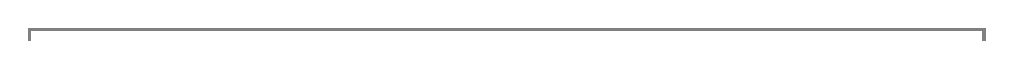
\begin{tikzpicture}
      \draw[very thick,color=gray] (0,-0.15) -- (0,0) -- (\textwidth,0) -- (\textwidth,-0.15);
    \end{tikzpicture}
    
    %\frame{
    \begin{minipage}{0.95\textwidth}%
      \input{./syntax-out/c/#3}%
      \smallskip
    \end{minipage}%
    %}
    
    
\begin{tikzpicture}
      \draw[very thick,color=gray] (0,0.15) -- (0,0) -- (\textwidth,0) -- (\textwidth,0.15);
    \end{tikzpicture}
    \caption{C Syntax for #2}%
    \label{#1}%
  \end{figure}%
}

\newcommand{\passyntax}[3] {%
  \begin{figure}[htbp]%
   \centering%
    
    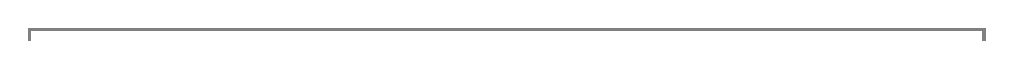
\begin{tikzpicture}
      \draw[very thick,color=gray] (0,-0.15) -- (0,0) -- (\textwidth,0) -- (\textwidth,-0.15);
    \end{tikzpicture}
    
    %\frame{
    \begin{minipage}{0.95\textwidth}%
      \input{./syntax-out/pascal/#3}%
      \smallskip
    \end{minipage}%
    %}
    
    
\begin{tikzpicture}
      \draw[very thick,color=gray] (0,0.15) -- (0,0) -- (\textwidth,0) -- (\textwidth,0.15);
    \end{tikzpicture}
    \caption{Pascal Syntax for #2}%
    \label{#1}%
  \end{figure}%
}

\newcommand{\examplesyntax}[3] {%
  \begin{figure}[htbp]%
   \centering%
    
    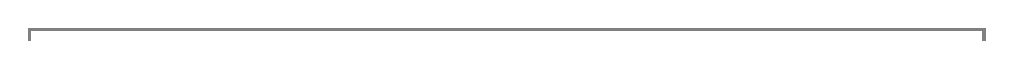
\begin{tikzpicture}
      \draw[very thick,color=gray] (0,-0.15) -- (0,0) -- (\textwidth,0) -- (\textwidth,-0.15);
    \end{tikzpicture}
    
    %\frame{
    \begin{minipage}{0.95\textwidth}%
      \input{./syntax-out/example/#3}%
      \smallskip
    \end{minipage}%
    %}
    
    
\begin{tikzpicture}
      \draw[very thick,color=gray] (0,0.15) -- (0,0) -- (\textwidth,0) -- (\textwidth,0.15);
    \end{tikzpicture}
    \caption{#2}%
    \label{#1}%
  \end{figure}%
}






% =======================
% = Drop Caps and Fonts =
% =======================

\usepackage{lettrine}

% ============
% = Glossary =
% ============
\usepackage[xindy]{glossaries}

% ==============================================
% = Packages required for Source Code Listings =
% ==============================================

\usepackage{listings}
\usepackage{upquote}
\usepackage{fancyvrb}
\usepackage{pdflscape}

\lstdefinelanguage[FPC]{Pascal}[Standard]{Pascal}
  {morecomment=[l]//,
   morekeywords={uses,external,cdecl,export,forward,global,module,nil,operator,overload,%
      priority,sum,type,use,dispose,mark,page,release,%
      eof,eoln,ord,pos,pred,rval,succ,result,interface,implementation,unit}%
  }%

\lstset{keywordstyle=\color{Blue}}
\lstset{commentstyle=\color{OliveGreen}}
\lstset{stringstyle=\color{BrickRed}}
\lstset{basicstyle=\ttfamily\small}
\lstset{captionpos=t}
% \lstset{frame=trbl}
\lstset{fancyvrb=true}
\lstset{numberstyle=\footnotesize}
\lstset{showstringspaces=false}
\lstset{tabsize=2}
\lstset{captionpos=b}

\newcommand{\straightcode}[1]
{
  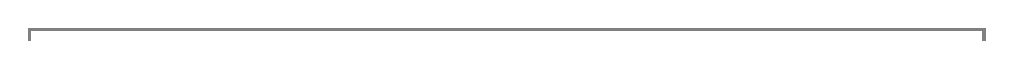
\begin{tikzpicture}
    \draw[very thick,color=gray] (0,-0.15) -- (0,0) -- (\textwidth,0) -- (\textwidth,-0.15);
  \end{tikzpicture}
  
  {#1}
  
  
\begin{tikzpicture}
    \draw[very thick,color=gray] (0,0.15) -- (0,0) -- (\textwidth,0) -- (\textwidth,0.15);
  \end{tikzpicture}
}


\newcommand{\pascode}[3]
{
  \lstset{language=[FPC]Pascal}
  \lstinputlisting[caption={#2},label={#1}]{#3}
}

\newcommand{\mpascode}[4]
{
  \lstset{language=[FPC]Pascal}
  \lstinputlisting[caption={#2},label={#1},multicols=#4]{#3}
}


\newcommand{\passnipet}[1]
{
  \lstset{language=[FPC]Pascal}
  \lstinline&#1&
}


\newcommand{\ccode}[3]
{
  \lstset{language=C}
  \lstinputlisting[caption={#2},label={#1}]{#3}
}

\newcommand{\mccode}[4]
{
  \lstset{language=C}
  \lstinputlisting[caption={#2},label={#1},multicols=#4]{#3}
}


\newcommand{\csnipet}[1]
{
  \lstset{language=C}
  \lstinline^#1^
}

\newcommand{\bashcode}[3]
{
  \lstset{language=bash}
  \lstinputlisting[caption={#2},label={#1}]{#3}
}

\newcommand{\bashsnipet}[1]
{
  \lstset{language=bash}
  \lstinline^#1^
}


\captionsetup[lstlisting]{labelfont=bf} 

\addtolength{\evensidemargin}{-0.50in}
\addtolength{\textwidth}{0.50in}

\addtolength{\topmargin}{-0.25in}
\addtolength{\textheight}{1.25in}

\usepackage{phdthesis}

% ==================
% = MyBox commands =
% ==================

\usepackage{lipsum,framed,color}

\definecolor{shadecolor}{rgb}{1,0.8,0.3}
\newlength{\boxwidth}
\newsavebox{\boxcontainer}

\newcommand\mybox[1]{%
  \begin{center}%
    \fcolorbox{black}{shadecolor}{%
      \begin{minipage}[t]{\dimexpr\textwidth-2\fboxsep-2\fboxrule}%
        #1%
      \end{minipage}}%
  \end{center}}

\newenvironment{Mybox}%
  {\begin{lrbox}{\boxcontainer}%
     \begin{minipage}{\dimexpr\textwidth-2\fboxsep-2\fboxrule}}%
  {\end{minipage}\end{lrbox}%
   \begin{center}%
     \fcolorbox{black}{shadecolor}{\usebox{\boxcontainer}}
   \end{center}}

\newenvironment{MyBox}{%
  \def\FrameCommand{\fcolorbox{black}{shadecolor}}%
  \MakeFramed{\setlength{\hsize}{\dimexpr\textwidth-2\fboxsep-2\fboxrule} \FrameRestore}}%
{\endMakeFramed}

% Settings for \mybox and Mybox
\setlength{\fboxrule}{0pt}
\setlength{\fboxsep}{9pt}

% Additional settings for MyBox
\setlength{\FrameRule}{\fboxrule}
\setlength{\FrameSep}{\fboxsep}

% ===========================
% = Bookmarks for PDF Index =
% ===========================
\usepackage[bookmarks=true,colorlinks=true,linkcolor=blue,plainpages=false,pdfpagelabels]{hyperref}

\newcommand{\cref}[1]{Chapter~\ref{#1}}
\newcommand{\sref}[1]{Section~\ref{#1}}
\newcommand{\fref}[1]{Figure~\ref{#1}}
\newcommand{\tref}[1]{Table~\ref{#1}}
\newcommand{\lref}[1]{Listing~\ref{#1}}
\newcommand{\eref}[1]{Equation~\ref{#1}}

% \usepackage[resetfonts]{cmap}
% 
% \begin{VerbatimOut}{OT1tt.cmap}
% %!PS-Adobe-3.0 Resource-CMap
% %%DocumentNeededResources: ProcSet (CIDInit)
% %%IncludeResource: ProcSet (CIDInit)
% %%BeginResource: CMap (TeX-OT1-0)
% %%Title: (TeX-OT1-0 TeX OT1 0)
% %%Version: 1.000
% %%EndComments
% /CIDInit /ProcSet findresource begin
% 12 dict begin
% begincmap
% /CIDSystemInfo
% << /Registry (TeX)
% /Ordering (OT1)
% /Supplement 0
% >> def
% /CMapName /TeX-OT1-0 def
% /CMapType 2 def
% 1 begincodespacerange
% <00> <7F>
% endcodespacerange
% 8 beginbfrange
% <00> <01> <0000>
% <09> <0A> <0000>
% <23> <26> <0000>
% <28> <3B> <0000>
% <3F> <5B> <0000>
% <5D> <5E> <0000>
% <61> <7A> <0000>
% <7B> <7C> <0000>
% endbfrange
% 40 beginbfchar
% <02> <0000>
% <03> <0000>
% <04> <0000>
% <05> <0000>
% <06> <0000>
% <07> <0000>
% <08> <0000>
% <0B> <0000>
% <0C> <0000>
% <0D> <0000>
% <0E> <0000>
% <0F> <0000>
% <10> <0000>
% <11> <0000>
% <12> <0000>
% <13> <0000>
% <14> <0000>
% <15> <0000>
% <16> <0000>
% <17> <0000>
% <18> <0000>
% <19> <0000>
% <1A> <0000>
% <1B> <0000>
% <1C> <0000>
% <1D> <0000>
% <1E> <0000>
% <1F> <0000>
% <21> <0000>
% <22> <0000>
% <27> <0000>
% <3C> <0000>
% <3D> <0000>
% <3E> <0000>
% <5C> <0000>
% <5F> <0000>
% <60> <0000>
% <7D> <0000>
% <7E> <0000>
% <7F> <0000>
% endbfchar
% endcmap
% CMapName currentdict /CMap defineresource pop
% end
% end
% %%EndResource
% %%EOF
% \end{VerbatimOut}

% If you want to generate a toc for each chapter (use with book)
\usepackage{minitoc}

\setcounter{totalnumber}{50}
\setcounter{topnumber}{50}
\setcounter{bottomnumber}{50}

\renewcommand\floatpagefraction{.9}
\renewcommand\topfraction{.9}
\renewcommand\bottomfraction{.9}
\renewcommand\textfraction{.1}

% ============
% = Metadata =
% ============

\title{The Programming Arcana}
\author{Andrew Cain}
\date{\today}


% \includeonly{topics/preface/preface}
\includeonly{topics/0-getting-started/getting-started}
% \includeonly{topics/programs-and-compilers/compilers}
% \includeonly{topics/program-creation/program-creation}
% \includeonly{topics/storing-using-data/storing-using-data}
% \includeonly{topics/control-flow/control-flow}
% \includeonly{topics/arrays/arrays}
% \includeonly{topics/type-decl/type-decl}
% \includeonly{topics/dynamic-memory/dynamic-memory}
% \includeonly{topics/file-io/file-io}

\begin{document}
  \dominitoc 
  \dominilof 
  \dominilot
  
  \faketableofcontents
  \frontmatter
  \begin{titlepage}

  \begin{tikzpicture}[remember picture, overlay]
      \node[inner sep=0pt] at (current page.center) {%
          %\includegraphics[width=\paperwidth,height=\paperheight]{resources/images/ProgrammingArcanaTome}%
          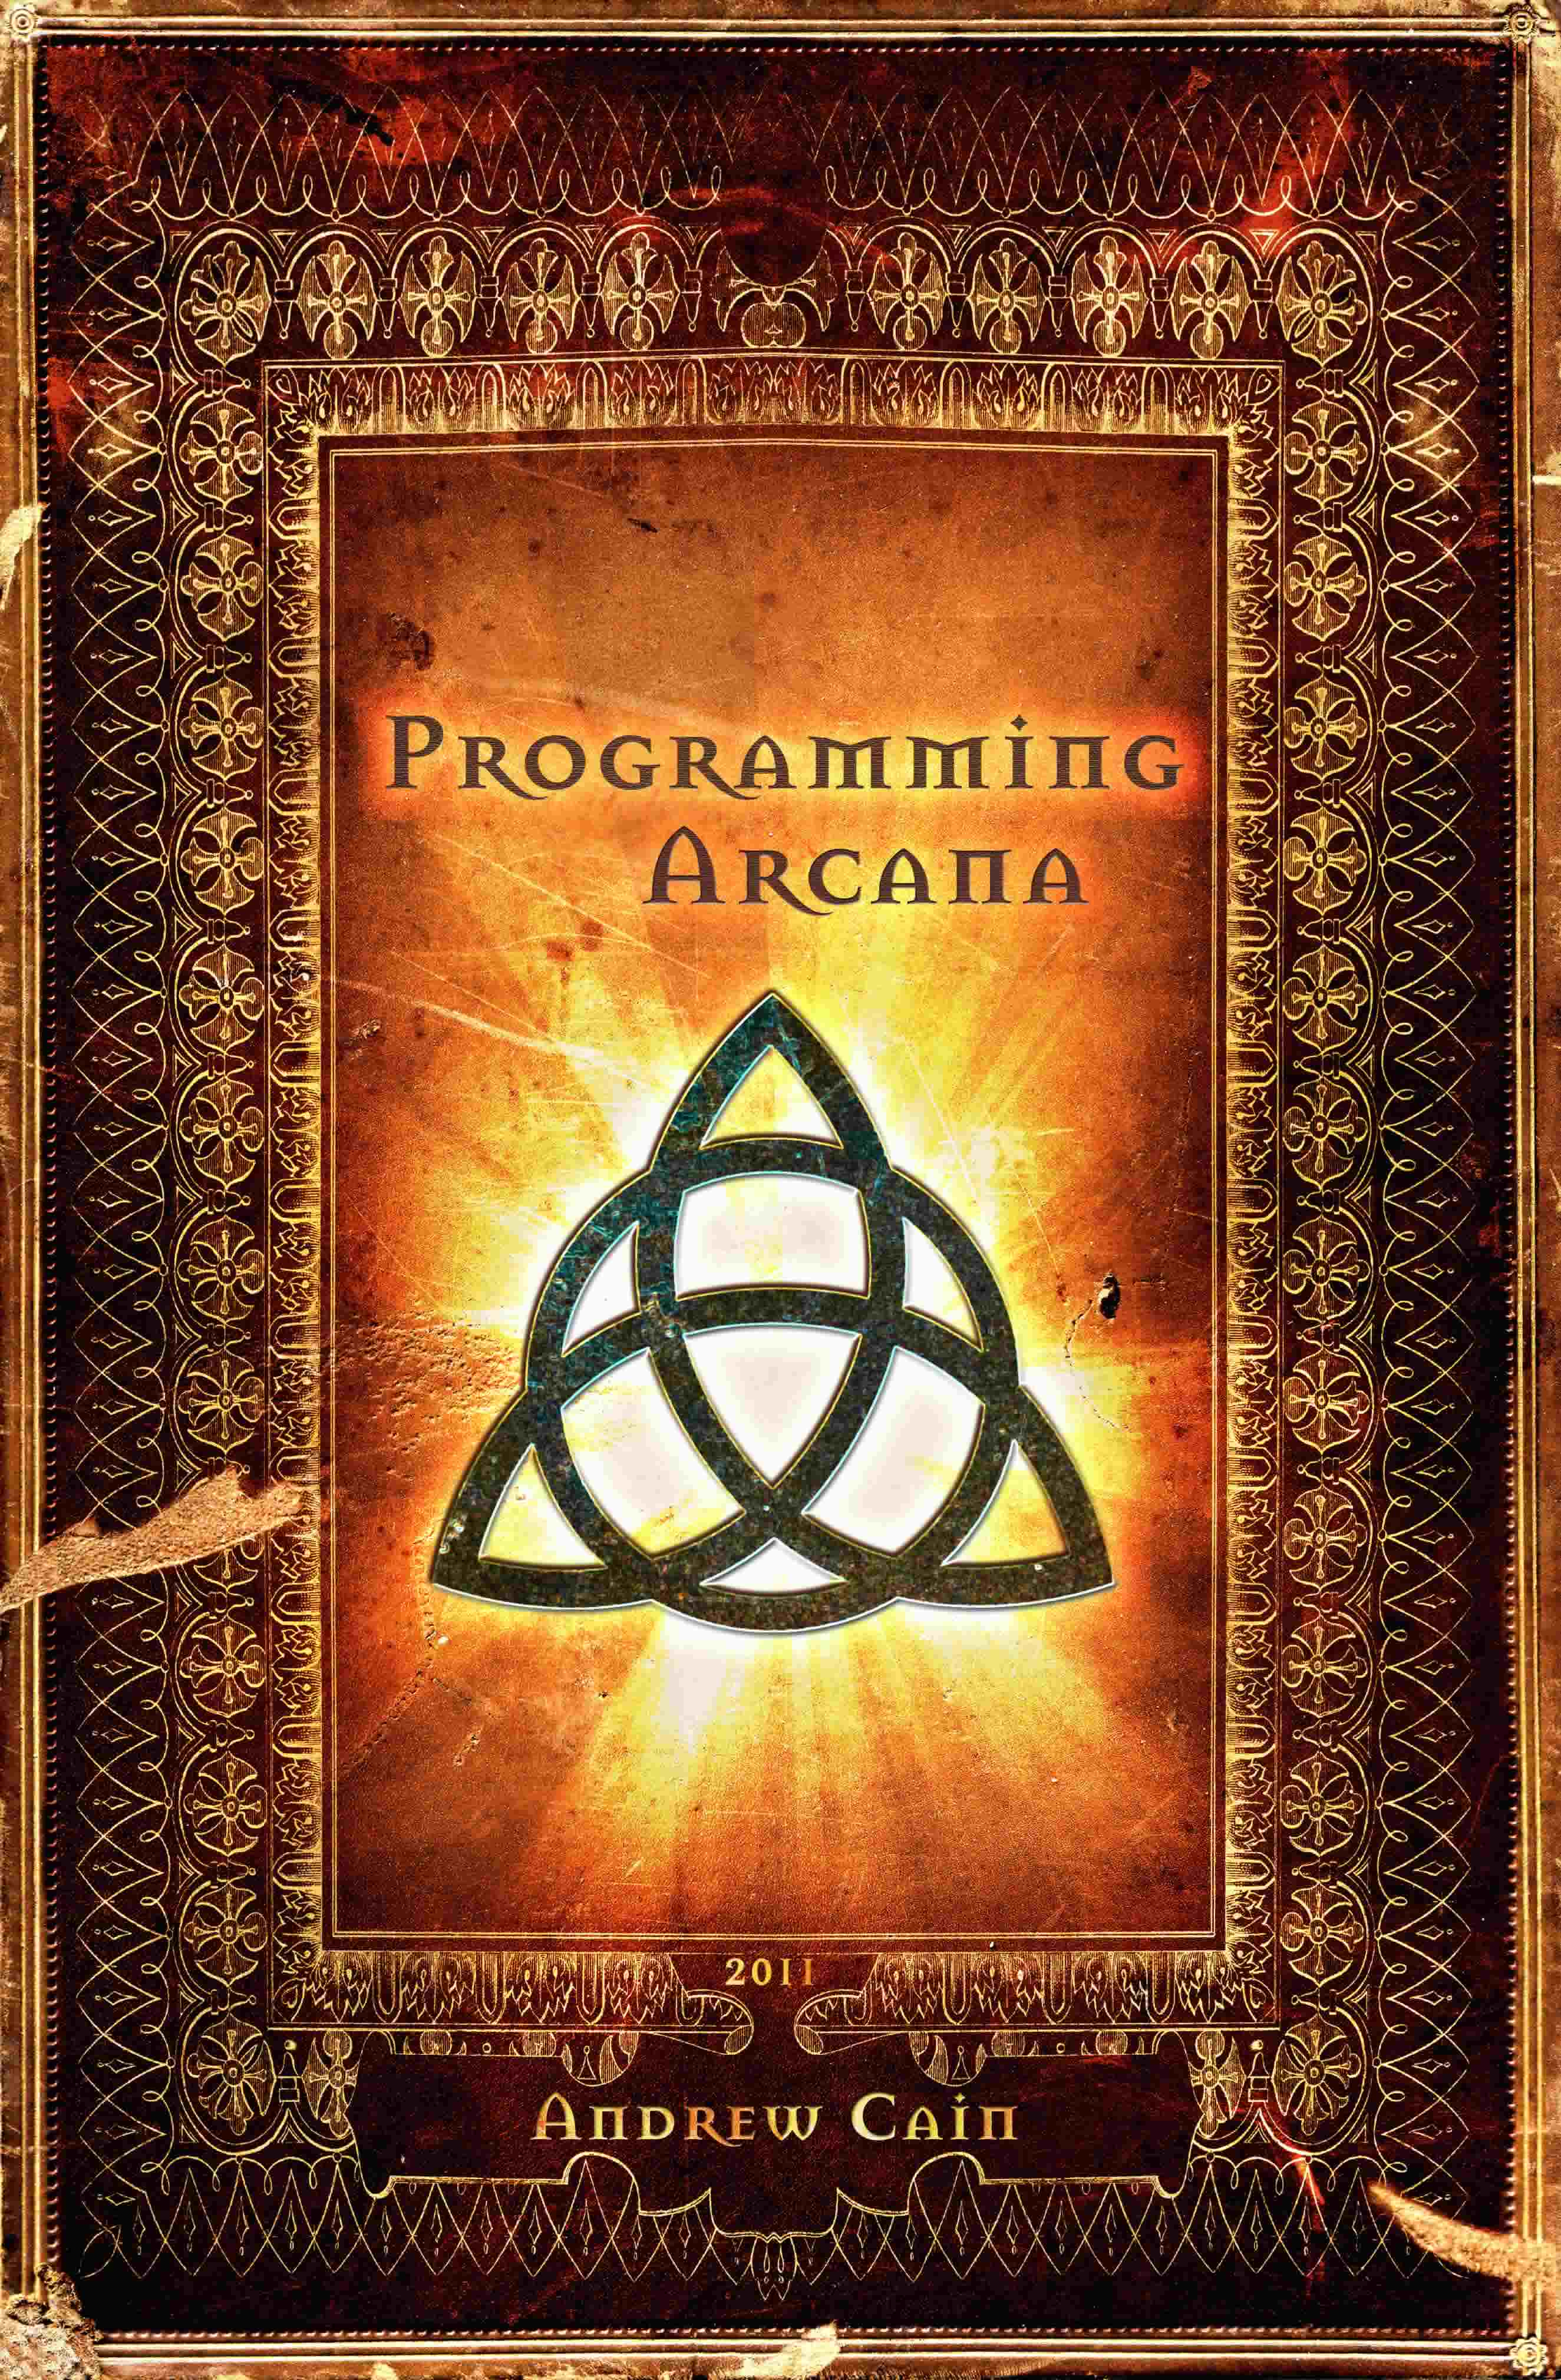
\includegraphics[width=\paperwidth,height=\paperheight]{resources/images/Tome1.jpg}%
      };%
  \end{tikzpicture}

\end{titlepage}
  
  \mainmatter
  \chapter*{Preface} % (fold)
\label{cha:preface}

\begin{quote}
  %\frakfamily\selectfont\Large
  \Fontlukas\Large
  \renewcommand{\LettrineTextFont}{\relax}
  \lettrine[image=true,lines=3,lraise=0.1]
  {W}{elcome} neophyte!  So you seek to master the arts of Magic. Well, you have come to the right place. Here we will give you the opportunity to explore magic, to understand its working and use. Before we start I have one piece of advice for you, practice, for it is only through practice that you can hope to learn these secret arts.
\end{quote}

\bigskip

Welcome to the Programming Arcana\footnote{Arcana is defined as secrets or mysteries, Wiktionary defines it as ``specialized knowledge that is mysterious to the uninitiated.''. This fits well with the idea of programming, and we think its a cool word to describe the \emph{magic} of programming!}, a book about learning to program. This book contains a number of chapters that take you from knowing nothing, or little, about programming to a position where the mysteries are revealed. By the end of the material you will be able to create your own programs and you will be ready to start learning other programming languages and approaches to software development.

This book is divided into a number of chapters, each of which introduces you to a programming task and the arcane knowledge that must be attained to understand how the task is accomplished. As with any arcane knowledge there are special terms that are used by those who know its secrets. In each chapter you will be introduced to the terms you need to understand in order to perform the current task. This will provide you with the tools you need to describe programs to other software developers, and will help you understand how the structures within your programs work to achieve their goals.

Before we start getting into details let us have a look at how you can use this book to help you become a master of the arcane arts of programming.

\section*{Book Overview} % (fold)
\label{sub:book_overview}

This book is designed for people who want to gain an in depth knowledge of software development. It assumes that you are familiar with computers and how to use them, but does not require you to have any prior programming experience. You should feel comfortable using a computer, and be prepared to start looking at how it works in more detail.

There are a number of different ways in which texts can present their material. In this book, the content is presented using a concept first approach. This approach places the programming concepts as the central focus, with details of syntax being secondary. The logic behind this is that you can learn new syntax if you understand the concepts, whereas it will be difficult to be productive if you understand the syntax but do not understand the concepts behind this syntax. To this end, this book gives you the choice to study either the C or Pascal programming language. Both languages are very capable, and offer different advantages and challenges.

The chapters of this book build upon each other. Each chapter covers a new group of concepts, that will expand your programming capabilities and enable you to create larger and more capable programs. The layout of each chapter is the same, with the concepts having the main focus. Each chapter is laid out in the following order:
\begin{enumerate}
  \item \textbf{Concepts}: The first part of the chapter introduces the concepts that will be covered. This is done in a language neutral manner, with the focus being on how to think about the tools being presented. This will introduce each concept with an illustration, and accompany this with explanatory text.
  \item \textbf{Using the Concepts}: The next section shows how these concepts can be used to achieve a task. This task will try to cover all the concepts presented in a practical manner. This is done in a language neutral way, and talks about how to use the concepts to achieve a goal.
  \item \textbf{Languages}: The next two sections present the syntax you need to use these concepts in \textbf{C} and \textbf{Pascal}. You should use this as a reference, and can read this alongside reading about how to use the concepts.
  \item \textbf{Understanding}: Following the language specific details, the next section explains in detail how the concepts work within the computer. Use this to get an understanding of how the concepts work in more detail. This section will show you illustrations of what is happening within the computer when your code is running.
  \item \textbf{Examples}: Each chapter will have at least one example showing you how these concepts can be used. This will include the code, and some explanatory text to discuss what is being presented.
  \item \textbf{Exercises}: The exercises allow you to put into practice what you have read about. You cannot learn to program without practice. These exercises are a good start, but you should try to come up with your own project so that you can test out these new concepts on something you are interested in working on.r
\end{enumerate}

\section*{Which Language?} % (fold)
\label{sec:which_language_}

A programming language defines a set of rules that determine how you write the code for your programs. Each language defines its own rules, and so there is always the temptation to focus heavily on these details and place the overriding concepts in second place. We believe that when you are starting to learn to program, a good understanding of the programming concepts is far more important than the details of the programming language you are using. This book is not an in depth study of either the C or Pascal language, it is a book about learning to program.

To really learn these concepts well you will need to practice putting them to use. This will require you to use a programming language. Each chapter will provide you with enough information to put the concepts to use in either the C or Pascal language. So the main question you need to answer now is which language will you use?

Both C and Pascal are very capable languages. Pascal was designed as a teaching language, which means that it does make it a little easier to see how the concepts being covered apply to your code. C, on the other hand, is a commercial language designed for professionals to build programs. This is both an advantage and disadvantage for C. The advantage is that the language is widely used in industry, but the disadvantage is that it lacks the clarity that is offered by Pascal. Remember that this is only your first programming language. A professional software developer will know many different languages, and by the end of this material you will be equipped to learn many new languages.

\csection{
C is a very flexible language that is widely used in industry, though its syntax is more of a challenge to learn.
}

\passection{
Pascal is a powerful languages that was designed to teach programming. It is used in industry, but not to the same extent as C.
}

% section which_language_ (end)

\clearpage
\section*{Formatting} % (fold)
\label{sub:formatting}

This book has a number of visual formatting guides. These are designed to help you navigate through the material easily.

\pseudosection{
Text formatted in this way relates to an algorithm description. This will describe the steps that need to be performed in a way that is language neutral and can be applied to C, Pascal, and possibly other languages.
}

\csection{
Text formatted in this way relates to the C programming language. If you are going to use C you need to pay attention to the text in these boxes, otherwise you can skip over them.
}

\passection{
Text formatted in this way relates to the Pascal programming language. If you are going to use Pascal you need to pay attention to the text in these boxes, otherwise you can skip over them.

}

\mynote{
Text formatted in this way covers notes related to the current concept or illustration. This book makes extensive use of notes to capture important points, so do not skip over these.
}

The language sections of each chapter also add markers to each page to clearly mark where they start, and where they end. If this is your first programming experience you should stick with one of these languages, so you can skip the pages that are marked as being for the other language.


% subsubsection formatting (end)


% subsection book_overview (end)

% \clearpage
\section*{Programming Jargon and Concept Taxonomy} % (fold)
\label{sub:concept_taxonomy}

Programming has a lot of its own jargon. As you learn to develop software it is also important that you start to learn this \emph{special language} that software developers use to discuss their programs. You will find that this terminology is used in many places. It is used in programming texts, in discussions between developers, in discussion boards, blogs, anywhere that developers are discussing software development. Having a clear understanding of this terminology will help you make the most of these resources.

The concepts in this book are closely linked to this programming terminology. To help you understand each concept, we have classified them using one of the following categories:

\begin{itemize}
  \item \textbf{Artefact}: An artefact is something that you can create in your code.
  \item \textbf{Action}: Actions are things that you can \emph{command} the computer to do.
  \item \textbf{Term}: These are general terms, used to describe some aspect.
\end{itemize}

When you are reading about the different concepts in this book you can use these classifications to help you think about how you may use the knowledge you are gaining.

\paragraph{Artefacts:} % (fold)
\label{par:artefacts}

Artefacts are things that you create in your code. Programming is a very \emph{abstract} activity, you spend most of your time working with concepts and ideas. You write text, code, that will create things within the computer when your code is run. 

When you are learning about a new kind of artefact come up with ways of visualising it. It is a \textbf{thing} that you are creating with your code. Try to picture the artefact within your code. These artefacts are the basic building blocks that you have to work with. You need to be very familiar with them, how they work, and what you can do with them.

% subsubsection artefacts (end)

\paragraph{Actions:} % (fold)
\label{par:actions}

Actions get the computer to perform a task. Your actions will be coded within the \textbf{artefacts} that you create, and will define how artefacts behave when they are used. The actions themselves are commands that you issue to the computer. They are executed one at a time, and each kind of action gets the computer to carry out certain tasks.

When you are learning a new kind of action you need to see what this action does. To start with you should play with it, test it out, and see if you can understand what it is getting the computer to do. As you progress you need to start thinking about how you can sequence these actions so that the computer performs the tasks you want it to. There are only a very few kinds of actions, so it is by combining them that you can get the computer to do what you want. 

% subsubsection actions (end)

\paragraph{Terms:} % (fold)
\label{par:terms}

The remaining terms are words that developers use to explain concepts. These are not things that you create, or actions that you request. These are just words that you need to \emph{know}.

When you are learning a new term you need to try to commit it to memory. Memorise the terms, try to use them in sentences, explain them to others. All of these tasks will help you understand, and remember these terms.

% subsubsection terms (end)

% subsection concept_taxonomy (end)

\section*{Advice} % (fold)
\label{sec:advice}

If you want, or need, to learn to program then you can not do this just by reading a book, even one as magical as this. Learning to program requires practice. This book is designed to give you the concepts you need in order to understand how to go about creating your first programs. To really understand these concepts you need to apply them to the creation of your own programs.

When you are getting started, programming can appear quite daunting and the tools you use can be unforgiving. Work through these initial challenges, and with practice you will be able to overcome them. Once you have some success there is nothing better than seeing a program you created running on a computer. You have brought the machine to life, getting it to perform a task the way you want it performed. Once you get a program working it can become easy to get hooked and working on new features and functions becomes a real joy. The greater the challenge the program offers, the greater your sense of achievement when you see the working product in operation.

Other people are the best resources to help you get over these initial challenges. Fellow students studying this material can provide you with support, and a chance to discuss the challenges you are facing. Teaching staff are also a good resource when you are really stuck. If you do not have access to anyone who can help, use discussion boards and websites. Getting the right help will make a large difference to your learning experience.

Remember that you will need to study this material. That is not just reading it, but thinking and reflecting on what you have read. Try to think about each of the concepts, and how they relate to the other material that has been presented to you. Try to design and build your own programs with the material you are learning. If you do think deeply and apply the concepts to programs you create, you will eventually get the light bulb moment when things become clear and programming can become truly joyful.

% section advice (end)

% chapter preface (end)

  % 0 - Getting Started
  % 1 - Programs: Commands, Data, and Sequence
  % 2 - Procedures and Parameters
  % 3 - Functions
  % 4 - Control Flow
  % 5 - Custom Types
  % 6 - Arrays
  % 7 - Dynamic Memory
  % 8 - Program Design
  % 9 - Object Oriented Programming


  % 3 - Parameters: Pass by Reference

  % 1 - Sequence and Procedure Calls
  % 2 - Procedure declaration
  % 2 - Storing and Using Data
  % 3 - Parameters and Pass By Reference
  % 3 - Control Flow
  % 4 - Custom types
  % 5 - Arrays
  % 6 - Dynamic Memory 

  \setcounter{chapter}{-1}
\chapter{Getting Started} % (fold)
\label{cha:getting-started}

\begin{quote}
  \Fontlukas\Large
  \renewcommand{\LettrineTextFont}{\relax}
  \lettrine[image=true,lines=3,lraise=0.1]
  {M}{agic} requires both knowledge and tools. Our first lesson will uncover the tools of the Magi. Tools that you will need to use to practice magic. Here, take this ancient wand this orb and caldron. Each of these tools is essential to the working of even the most basic spells. Now lets see if you can wield that wand. Take it in your hand like this, and \ldots
\end{quote}

\bigskip

Software development requires both knowledge and tools. This first chapter introduces key details of your computer, how programs are created and run, and the tools you will use to build your own software.

When you have understood the material in this chapter you will be able to create programs from source code, run your programs, and identify cause of errors when creating or running your program.

\minitoc

% ====================================
% = Learning Focus - Getting Started =
% ====================================
\clearpage
\section{Learning Focus}
Programming is about providing instructions to get a computer to do the things that you want. In order to learn how to do this we need to start by understanding a little about the computer and how it works. This first chapter focuses on developing your understanding of how the computer works, how programs are created, and how they run. When you have successfully understood the material in this chapter you will be able to:

\begin{itemize}
  \item Describe key components of your computer, and how they relate to program execution.
  \item Describe the environment within which programs execute, and how this can impact on programs working.
  \item Setup a computer to build and run programs.
  \item Run programs from the command line.
  \item Setup and use a code editor to create small programs.
  \item Compile programs from the command line.
\end{itemize}

Once you have achieved these learning outcomes the next chapter will help you start to explore the key concepts for the components within a program.

% =====================================
% = Concepts - Compilers and Programs =
% =====================================

\section{Concepts Related to Getting Started}
\label{sec:concepts_related_to_getting_started}

There are two big questions we need to address here:

\begin{enumerate}
  \item What are programs?
  \item How can you create a program?
\end{enumerate}

\subsection{What are programs?}

\subsection{How can you create a program?}


\section{Understanding Getting Started}
\label{sec:understanding_getting_started}



\section{Secrets of the Magi -- Advanced Shell Usage}


  % \chapter{Building Programs} % (fold)
\label{cha:building programs}

\begin{quote}
  %\frakfamily\selectfont\Large
  \Fontlukas\Large
  \renewcommand{\LettrineTextFont}{\relax}
  \renewcommand{\LettrineFontHook}{\color{red}}
  \lettrine[image=true,lines=1,lhang=.2, loversize=.25, findent=0.1em]
  {W}{elcome} neophyte! So you seek to master the art of Magic? To work magic you must learn the structure of incantations, and how to use a wand to convert these into magic energy. 
  
  Let us begin with a simple spell, a spell that will greet the world around you! Utter these words, and wave your wand\ldots
\end{quote}

\bigskip

Welcome to the Programming Arcana\footnote{Arcana is defined as secrets or mysteries, Wiktionary defines it as ``specialized knowledge that is mysterious to the uninitiated.''. This fits well with the idea of programming, and we think its a cool word to describe the \emph{magic} of programming!}, a book about learning to program. This book contains a number of chapters that take you from knowing nothing, or little, about programming to a position where the mysteries are revealed. By the end of the material you will be able to create your own programs and you will be ready to start learning other programming languages and approaches to software development.

This book is divided into a number of chapters, each of which introduces you to a programming task and the arcane knowledge that must be attained to understand how the task is accomplished. As with any arcane knowledge there are special terms that are used by those who know its secrets. In each chapter you will be introduced to the terms you need to understand in order to perform the current task. This will provide you with the tools you need to describe programs to other software developers, and will help you understand how the structures within your programs work to achieve their goals.

Like magic, you must learn the structure of source code, and how to use tools to convert these into programs. Let us begin with a simple program, a program that will greet the world.

\minitoc

% =====================================
% = Concepts - Compilers and Programs =
% =====================================
\clearpage
\section{Concepts Related to Building Programs} % (fold)
\label{sec:concepts_related_to_building_programs}

In this chapter you will learn about the basic tools you need to use to create your own programs. You will see an example program, and then use these tools to convert that code into an executable program. You will then be able to run the program you created, and see it perform the tasks you coded.

This chapter provides a background on what programs are, and the general processes of how they are created. This will introduce you to the tools you will be using, and fill in some details of what they are doing and how to use them. The topics covered include the following:
\begin{itemize}
  \item \nameref{sub:what_is_a_program_}: This section introduces you to the idea of what a program is, and what it contains. You will need to be familiar with programs and what they are, as you will need to be able to create your own.
  \item \nameref{sub:machine_code}: Talks about the kinds of instructions the computer understands, and why it is not very productive to work at this level. You need to understand that this exists behind the scenes, but do not need to be overly familiar with it.
  \item \nameref{sub:assembly}: The next level of language is called Assembly. It is very close to machine code, but much easier to understand and use. However, this is still too low a level to be very productive. Just like machine code, you only need to know this exists
  \item \nameref{sub:source_code_and_the_compiler}: This is the level we are going to be working with in this book. This code is much easier to work with than assembly, and allows you to create your own programs reasonably quickly once you have learnt the basics. These are the tools you are going to be working with throughout this text.
  \item \nameref{sub:terminal}: This is a command line environment that lets you issue text commands to the user. You will use this to create and run your programs.
  \item \nameref{sub:hello world}: A \emph{classic} program used to check that you have everything working correctly. This section shows you the code that you can use this to check that you have all the tools setup correctly, and to check their usage.
  \item \nameref{sub:compiling_code}: This final section will show you how to use these tools to compile and run your own Hello World program. \fref{fig:run-1-helloworld} shows the Hello World program running from the Terminal.
\end{itemize}

\begin{figure}[b]
   \centering
   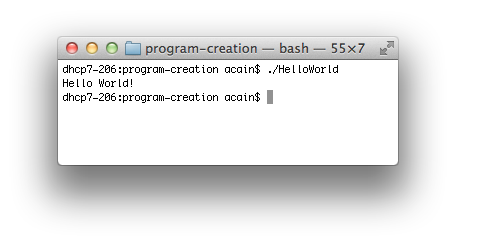
\includegraphics[width=0.7\textwidth]{./topics/programs-and-compilers/images/HelloWorld} 
   \caption{Hello World run from the Terminal}
   \label{fig:run-1-helloworld}
\end{figure}


\clearpage
\subsection{Programs} % (fold)
\label{sub:what_is_a_program_}

If you are going to learn to develop software you will need to become intimately aware of what a program is. After all, as a developer you will be creating your own programs.

A program is a file that contains instructions that get the computer to perform a task. Programs are lists of commands\footnote{C and Pascal are both \emph{imperative} programming languages. In the imperative paradigm a program is seen as a list of commands instructing the computer to perform actions.} telling the computer what to do, and the order in which to do it. Each instruction is very simple, but they can be executed very quickly, allowing computers to perform quite remarkable feats.

\begin{figure}[h]
   \centering
   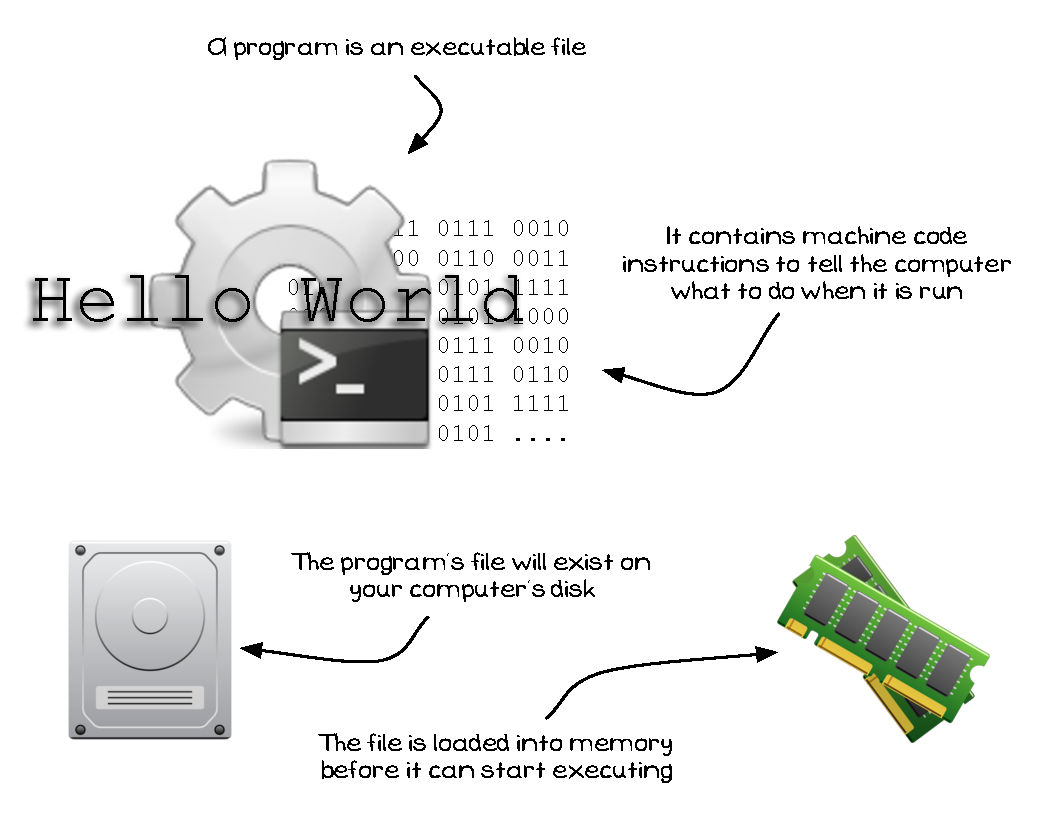
\includegraphics[width=0.9\textwidth]{./topics/programs-and-compilers/diagrams/Program} 
   \caption{A program contains instructions that command the computer to perform a task}
   \label{fig:what-is-a-program}
\end{figure}

\mynote{
\begin{itemize}
  \item You can \textbf{run} programs, which gets the computer to follow the instructions found within the program's file.
  \item To run, the program's instructions must first be loaded into memory.
  \item Once in memory, the computer starts running the instructions one after the other.
  \item When the last instruction is completed the program ends.
  \item There are several different ways to run a program:
  \begin{itemize}
    \item You can \emph{double-click} the program in a file browser.
    \item On tablets and app-phones you can \emph{tap} the program's icon.
    \item Advanced uses can enter \emph{text commands} in the Terminal to start programs.
  \end{itemize}
\end{itemize}
}

\clearpage
\subsubsection{What happens when a program runs?} % (fold)
\label{ssub:what_happens_when_a_program_runs_}

When you run a program, regardless of how it is started, the Operating System loads it from disk into memory and then starts it running. It is important that the file you try to run is a program. These are \emph{special} files that contain instructions the computer can understand.

\begin{figure}[h]
   \centering
   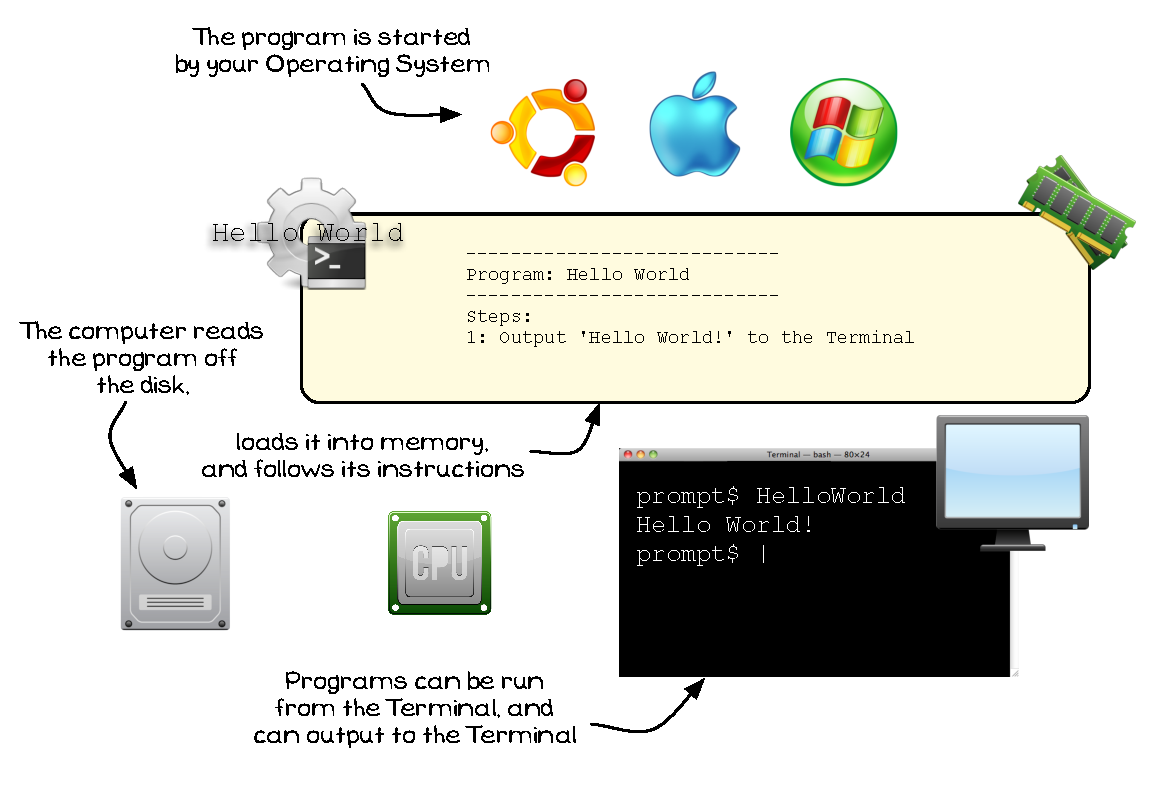
\includegraphics[width=0.9\textwidth]{./topics/programs-and-compilers/diagrams/ProgramExe} 
   \caption{Programs are loaded from disk into memory, then run}
   \label{fig:what-is-a-program-exe}
\end{figure}

\mynote{
\begin{itemize}
  \item Your Operating System is a piece of software that is responsible for managing your computer's hardware.
  \item One of the Operating System's responsible is to start programs.
  \item The \nameref{sub:terminal} can be used to start programs.
  \item Programs can also output to the Terminal.
  \item A Program must contain instructions that the computer can understand.
\end{itemize}
}

% subsubsection what_happens_when_a_program_runs_ (end)

% subsection what_is_a_program_ (end)
\clearpage
\subsection{Machine Code} % (fold)
\label{sub:machine_code}

\emph{What instructions do Computers understand?}

Computers do not really \emph{understand} anything, computers are \textbf{unintelligent}. They are a machine that respond in a set way to a given number of instructions. The instructions that a computer uses is called its {\em instruction set} and contain instructions to perform basic mathematic operations, loading and storing data in memory, comparing numeric values, and moving to the new instruction elsewhere in the program. These very simple actions are performed very quickly, and can be use to create everything you have ever seen a computer do.

The computers instructions can be seen as binary numbers, numbers made from 0's and 1's. These values are like switches that are either off (0) or on (1). Setting these \emph{switches} to different sequences will cause the computer to perform different actions. For example, the \emph{switch} combination \texttt{0000 0011}, may cause the computer to add two numbers together. Any time you want the computer to perform this task you set the switches to that combination. These binary instructions are called \textbf{machine code}.

\begin{figure}[h]
   \centering
   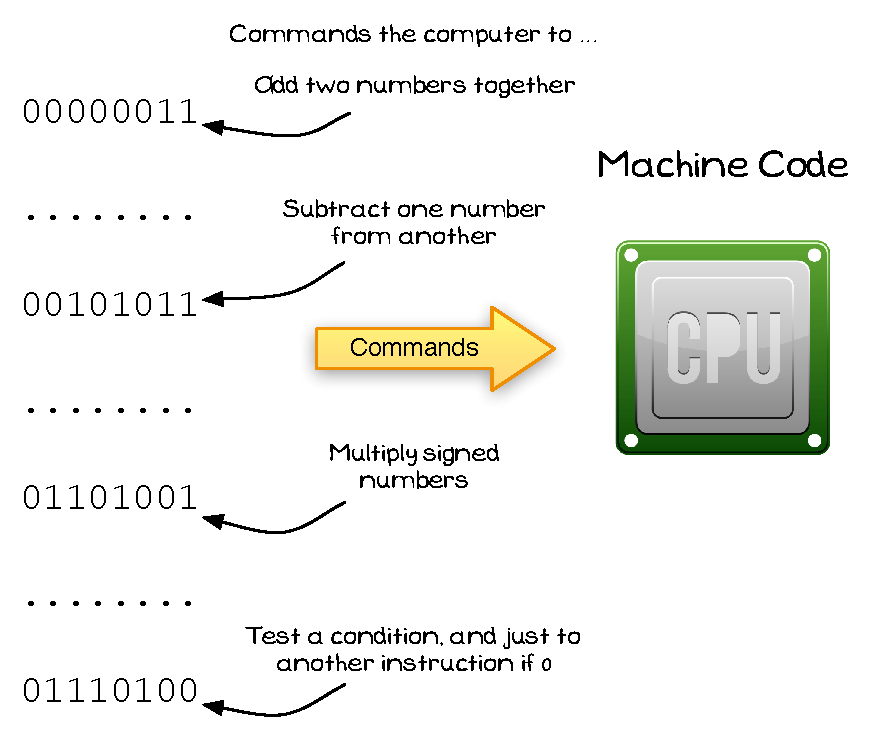
\includegraphics[width=0.8\textwidth]{./topics/programs-and-compilers/diagrams/MachineCode} 
   \caption{The computer responds to machine code instructions}
   \label{fig:machine-code}
\end{figure}

\mynote{
\begin{itemize}
  \item The \textbf{CPU}, Central Processing Unit, is the workhorse of the computer. It executes the program's instructions.
  \item The instructions a CPU uses is called its \textbf{Instruction Set}, and different CPUs have different instruction sets.
  \item Some common instruction sets: ARM (used in iPhones and iPads), x86-64 (used in desktops), and PowerPC (used in the XBox360 and Playstation 3). 
\end{itemize}
}

\clearpage

\subsubsection{Programming in Machine Code} % (fold)
\label{ssub:programming_in_machine_code}

Listing \ref{lst:machine code} shows a chunk of the machine code for a small program. These 1s and 0s are the codes used to instruct the computer when this program is executed. Programs can be written directly in machine code, but this is a time consuming task. This is further complicated by the fact that machine code is unique to each kind of CPU. This means that programming at this level is entirely dependent on the kind of processor that you are targeting.

\begin{lstlisting}[caption={128 bits from the 106,752 bits of Machine Code from a small program.},label={lst:machine code}]
...
0110 0111 0111 0010 0000 0000 0110 0011 0100 1110 0101 1111 0100 0001 0101 1000
0110 0111 0111 0010 0000 0000 0111 0110 0101 1111 0101 1111 0110 1001 0101 1111
...
\end{lstlisting}

No one wants to have to work at this level of details, and fortunately you do not need to. Software developers have created tools to help them create programs without having to think about these low level details. These tools make it possible to work at a \textbf{higher level of abstraction}. They take the code you write, and do the hard work of converting that to the machine code of the computer you want to run it on.

\mynote{
\begin{itemize}
  \item You can look at the machine code of any program on your computer. You just need the right tools.
  \item If you open the program's executable file in a text editor it will look very strange, and not at all like a large list of binary values. This is because the text editor displays one character for every byte (or two bytes depending on the file) from the file.
  \item A \textbf{Hex Editor} is a program that is useful for examining binary data. It shows you one character for every four bits in the file.
\end{itemize}
}

\begin{table}[h]
  \ttfamily
  \centering
\begin{tabular}{|c|c||c|c||c|c||c|c|}
  \hline
  Binary & Hex & Binary & Hex & Binary & Hex & Binary & Hex  \\
  \hline
  0000 & \textbf{0} & 0001  & \textbf{1}  & 0010  &  \textbf{2} & 0011 & \textbf{3} \\
  0100 & \textbf{4} & 0101 & \textbf{5} & 0110 & \textbf{6} & 0111 & \textbf{7} \\
  1000 & \textbf{8} & 1001 & \textbf{9} & 1010 & \textbf{A} & 1011 & \textbf{B} \\
  1100 & \textbf{C} & 1101 & \textbf{D} & 1110 & \textbf{E} & 1111 & \textbf{F} \\
  \hline
\end{tabular}
  \caption{Binary to Hexadecimal}
\end{table}

\begin{figure}[h]
   \centering
   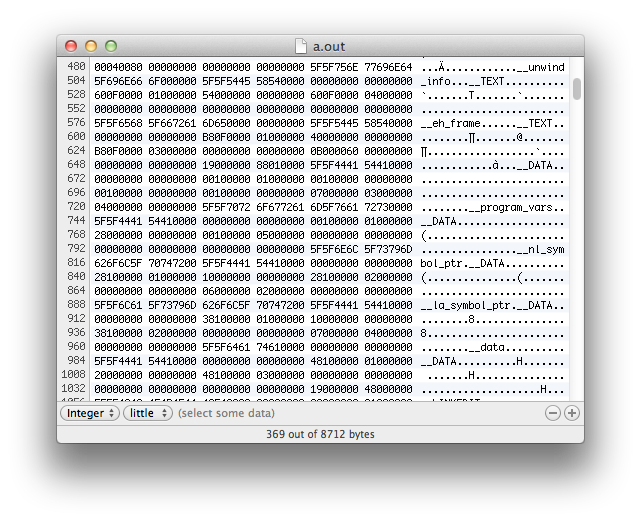
\includegraphics[width=0.55\textwidth]{./topics/programs-and-compilers/images/HexEditor} 
   \caption{A HexEditor allows you to view the machine code of any program}
   \label{fig:hex-editor}
\end{figure}


% subsubsection programming_in_machine_code (end)

% subsection machine_code (end)
\clearpage
\subsection{Assembly} % (fold)
\label{sub:assembly}

The next level of abstraction up from machine code is called \textbf{Assembly}, or \textbf{Assembler Code}. Here the numeric machine code instructions are given symbolic names that are, to some degree, more understandable for humans. The code \texttt{0000 0011} may be given the symbolic name \texttt{add}, for example.

Programs written in this language cannot be executed directly by the computer, it isn't machine code. Assembler code is converted to machine code by a program called an \textbf{Assembler}. This program reads the instructions from the assembler code and outputs machine code. So, for example, anywhere it encounters \texttt{add} in the code it can output \texttt{0000 0011}.

\begin{figure}[h]
   \centering
   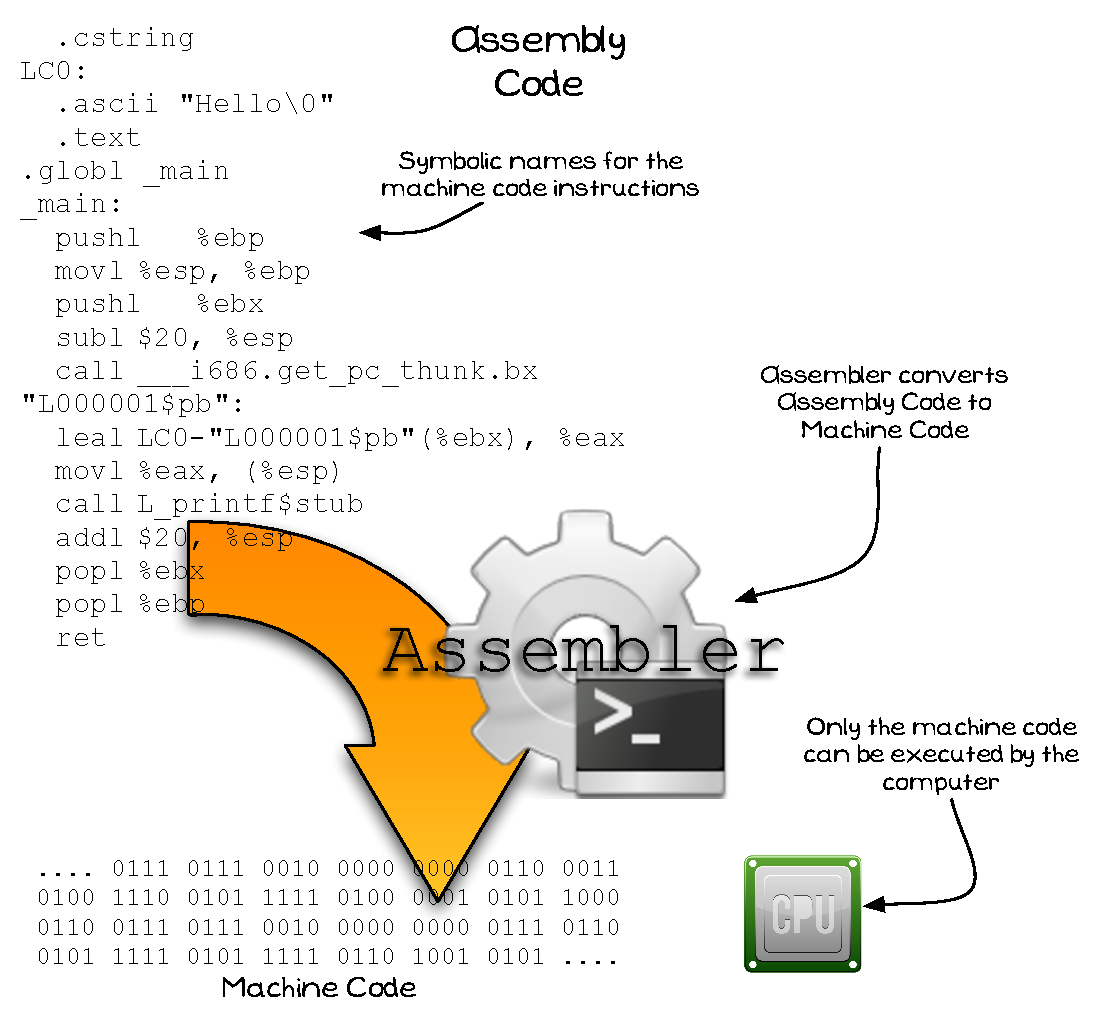
\includegraphics[width=0.8\textwidth]{./topics/programs-and-compilers/diagrams/Assembly} 
   \caption{The computer responds to machine code instructions}
   \label{fig:assembly}
\end{figure}

\mynote{
\begin{itemize}
  \item As with \nameref{sub:machine_code}, Assembly is liked to individual CPUs.
  \item Assembly is very close to Machine Code, its machine code with symbolic names for the instructions.
\end{itemize}
}

\clearpage
\subsubsection{Programming in Assembly} % (fold)
\label{ssub:programming_in_assembly}

The code in Listing \vref{asmcode} shows an example of some assembler code. This is the assembler code that was used to generate the machine code from Listing \ref{lst:machine code}. The machine code was 13,344 bytes in size, where the same program in assembler code is only 658 bytes. The assembler reads these 658 bytes, combines it with instructions from program libraries, and outputs machine code. 
\lstset{language=[x86masm]{assembler}}

\begin{lstlisting}[caption={Assembler Sample},label={asmcode}]
  .cstring
LC0:
  .ascii "Hello\0"
  .text
.globl _main
_main:
  pushl	%ebp
  movl	%esp, %ebp
  pushl	%ebx
  subl	$20, %esp
  call	___i686.get_pc_thunk.bx 
"L000001$pb":
  leal	LC0-"L000001$pb"(%ebx), %eax
  movl	%eax, (%esp)
  call	L_write_line$stub
  addl	$20, %esp
  popl	%ebx
  popl	%ebp
  ret
\end{lstlisting}

From a programmer's perspective, assembler code is much easier to work with than machine code, though there are still issues with the use of assembler code. Firstly Assembly is bound to the instruction set of the CPU that you are targeting, meaning that if you want to support other kinds of CPU you will need to rewrite the program. The other main issue with assembler code is that while it is more understandable, you are still working with the primitive instructions of the CPU. Working at this level takes considerable effort to write even simple programs.

Assembly languages were first developed in the 1950s, and were known as a \textbf{Second Generation}\footnote{First Generation being Machine Code.} programming languages. This step forward did make programming easier, but the tools have advanced since then and now we can work at an even higher level of abstraction.

% subsubsection programming_in_assembly (end)

% subsection assembly (end)
\clearpage
\subsection{Source Code and the Compiler} % (fold)
\label{sub:source_code_and_the_compiler}

The next step in programming language evolution moved from machine level instructions to something more human readable. These languages, known as \textbf{Third Generation Languages}, use move advanced programs than assemblers to convert their instructions into machine code. Programs written in these languages have their code converted to machine code by a \textbf{compiler}.

A \textbf{Compiler} is a program that converts \textbf{Source Code} into machine code that is saved into an executable file called a \emph{Program}. The program can then be executed independent of the compiler and the source code.

Internally, a compiler will perform a number of steps, as shown in \fref{fig:compiler}.

\begin{enumerate}
  \item \textbf{Preprocessing}: The code is read from your source code files. This may involve some processing of the text itself, which includes things like ignoring any comments in the code.
  \item \textbf{Compiling}: The code is then converted into assembly instructions, and an assembly program is output.
  \item \textbf{Assembling}: The assembly version of the program is converted into machine code, and stored in \textbf{object files}.
  \item \textbf{Linking}: In the final step the compiler uses a \textbf{Linker} to join together the machine code from your program, with other machine code you have used from the programming libraries. This then outputs an executable program.
\end{enumerate}

\begin{figure}[h]
   \centering
   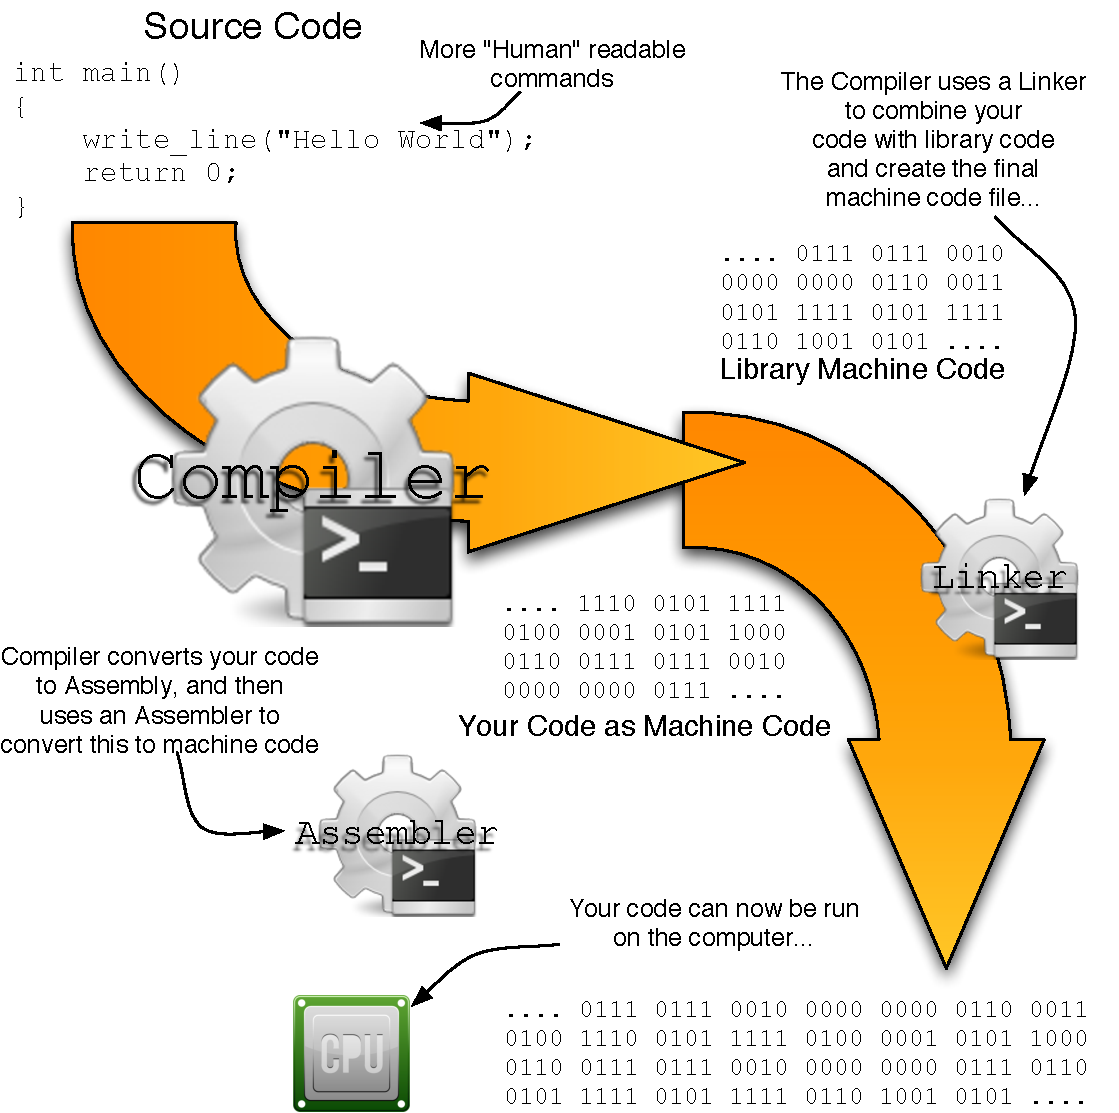
\includegraphics[width=0.8\textwidth]{./topics/programs-and-compilers/diagrams/Compiler} 
   \caption{Compilers turn Source Code into Machine Code}
   \label{fig:compiler}
\end{figure}

\clearpage
\subsubsection{Programming with a Third Generation Language} % (fold)
\label{ssub:programming_with_a_third_generation_language}

\lref{lst:hello-world-c-1} and \lref{lst:hello-world-pas-1} show two examples of source code. This code describes a small program that can be used to output a message to the \nameref{sub:terminal}.

\begin{multicols}{2}
  \ccode{lst:hello-world-c-1}{Example C code}{code/c/program-creation/hello-world.c}
  \columnbreak
  \pascode{lst:hello-world-pas-1}{Example Pascal code}{./topics/program-creation/pascal/HelloWorld.pas}
\end{multicols}

The code shown in \lref{lst:hello-world-c-1} shows the code for the C program that was used to generate the assembler code, and machine code shown in the previous code listings. This code must be converted by the C compiler into machine code before it can be run. It is interesting to note the size of the C file: it is only 50 bytes! The compiler converts this 50 bytes into the 13,344 bytes of machine code. 

\lref{lst:hello-world-pas-1} shows the same program written in the Pascal programming language. Like its equivalent C code, this must be compiled to create a program you can run.

Programs written in a third generation programming language are much easier to understand than their assembler or machine code counterparts. It is also possible that this code can be compiled to run on different types of CPU, making it more portable. Most modern programming languages are third generation programming languages.


The code that a programmer writes in these languages is called \textbf{Source Code}. Typically source code is saved into a text file with a file extension that helps identify the language it is written in. For example, programs written in the C language are saved into files with a {\tt .c} file extension whereas Pascal programs are saved into files with a {\tt .pas} extension.

\mynote{
\begin{itemize}
  \item There are may different Third Generation Languages, including both C and Pascal.
  \item Each language has its own compiler that understands that language's code.
  \item The C compiler we will use is called \textbf{gcc} - this stands for \textbf{GNU C Compiler}.
  \item The Pascal compiler we will use is called \textbf{fpc} - this stands for \textbf{Free Pascal Compiler}.
\end{itemize}
}



% subsubsection programming_with_a_third_generation_language (end)

% subsection source_code_and_the_compiler (end)
% \clearpage
\subsection{Challenges and Rewards} % (fold)
\label{sub:challenges_and_rewards}

% subsection challenges_and_rewards (end)

Programming in a third generation language, like C++ and Pascal, requires you to master several different things, as shown in the following list. The following chapters will work on building your knowledge and skills in each of these aspects.

\begin{enumerate}
  \item What is it that you want the program to do? Writing a program is like writing instructions for someone to carry out. If you do not know how to perform the task yourself you will not be able to tell someone else how to perform the task.
  \item You need to understand what the computer is capable of doing. Computers are unintelligent, so writing a program is more challenging than giving instructions to a person as the computer cannot interpret what you mean and will follow your instructions to the letter, regardless of the effect. The capabilities of the computer limit the flexibility you have for expressing your solution.
  \item The language you choose to develop with also limits how you express your solution. You need to understand the artefacts that you can create, how these artefacts are written in source code, and how these are executed by the computer.
  \item Finally you need to understand how to locate and correct issues with your programs. This includes responding to syntax errors reported to you by the compiler, as well being able to locate errors where the program does not operate the way you intended. 
\end{enumerate}

\emph{With all of these challenges, what appeal does software development have?}

There is nothing better than seeing a program you created running on a computer. You have brought the machine to life, getting it to perform a task the way you want it performed. Once you get a program working it can become easy to get hooked and working on new features and functions becomes a real joy. The greater the challenge the program offers, the greater your sense of achievement when you see the working product in operation.

% subsection compiling_code (end)
\clearpage
\subsection{Terminal} % (fold)
\label{sub:terminal}

Once you have written some source code, you need to be able to compile it. This means, you need to run the \textbf{compiler}, and give it your source code files to compile. The best way to do this when you really want to learn about programming, is to run the compiler directly yourself. To do this you needed to use a \textbf{Terminal} program.

The Terminal is a program that gives you command line access to the computer. With command line access you can enter text commands to start programs. These programs can output details back to the Terminal for you to read, and interactive programs can also read input from you via this same Terminal.

\begin{figure}[h]
   \centering
   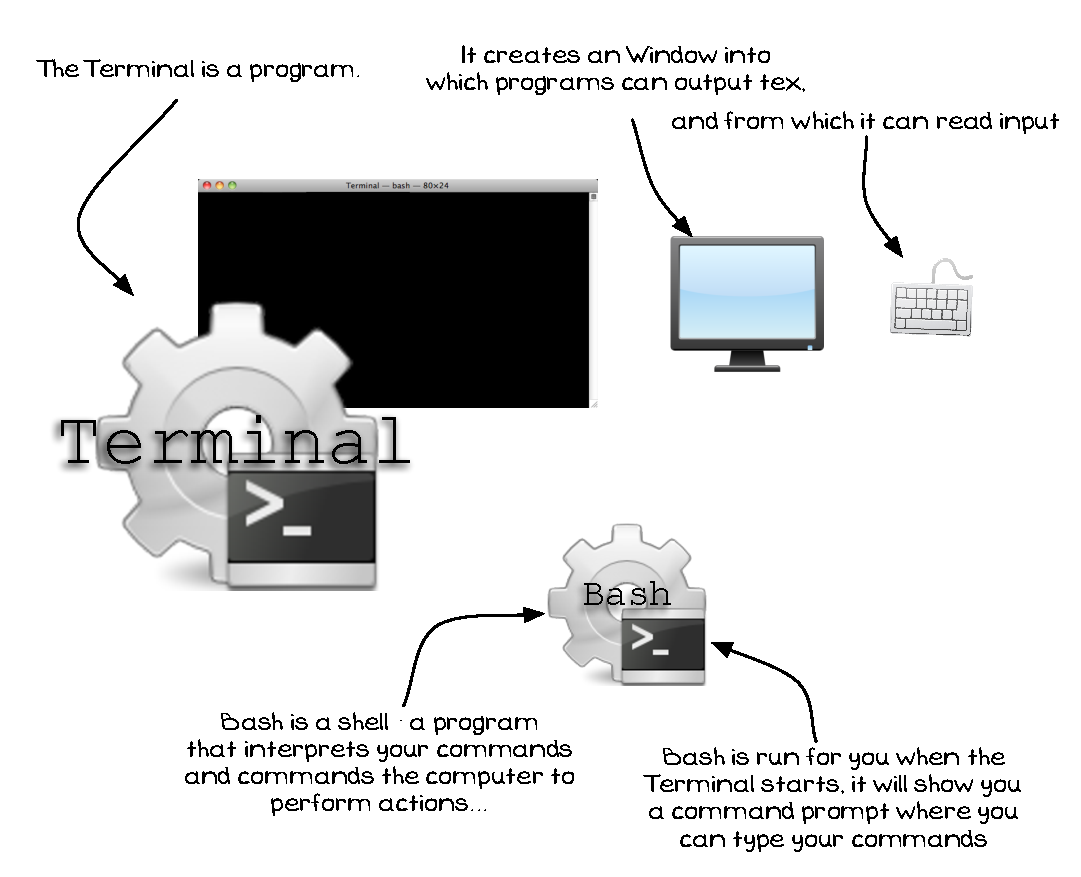
\includegraphics[width=0.8\textwidth]{./topics/programs-and-compilers/diagrams/Terminal} 
   \caption{The Terminal program gives you command line access to your computer}
   \label{fig:terminal}
\end{figure}

\mynote{
\begin{itemize}
  \item On Ubuntu \textbf{Linux} you can find the Terminal in the \emph{Accessories} folder within \emph{Applications}. See Figure \ref{fig:program-creation-ubuntu-terminal}.
  \item On \textbf{MacOS} you can find the Terminal in the \emph{Utilities} folder within \emph{Applications}. See Figure \ref{fig:program-creation-macos-terminal}.
  \item On \textbf{Windows} you will need to download and install \emph{MSys2}. The \emph{MSys2 Shell} is the equivalent of Terminal on the other operating systems. The details for how to install this are in the SplashKit installation guides.

  \item The Terminal is also be called the \textbf{console} or \textbf{command prompt}.
\end{itemize}
}

\clearpage
\subsubsection{The Shell} % (fold)
\label{ssub:the_shell}

The \textbf{Terminal} program itself just provides a text environment, allowing text input and output. Within this environment a \textbf{Shell} program is run to interpret your commands. This is an interactive program that will display a prompt to you, at which you enter your commands.

There are a number of different Shell programs, each of which has its own set of instructions. The Shell we are going to use in this book is called \textbf{Bash}. This shell program is available on Linux, Mac OS, and Windows. As a Unix shell it is native for Linux and Mac OS, and with Windows you can install \textbf{MSys2} to use these commands.

\begin{figure}[h]
   \centering
   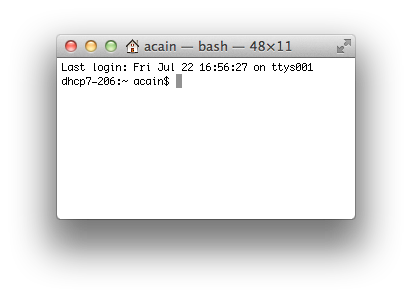
\includegraphics[width=0.6\textwidth]{./topics/programs-and-compilers/images/Bash} 
   \caption{The Terminal running Bash}
   \label{fig:bash}
\end{figure}

A shell program is very simple. It provides a text prompt at which you can enter commands. The Shell then reads the text you entered, and performs an action based on the text you entered. You can use the Shell to perform operations like copying and deleting files, and starting programs.

\mynote{
\begin{itemize}
  \item The name `Shell' came from idea that this was the outermost \emph{shell} of the computer, the interface between the user and the computer's internals.
  \item Bash stands for `\emph{Bourne-again shell}', as Bash is a replacement for the \emph{Bourne} shell.
  \item It will take some time to get used to using Bash, but the more you learn about it the more useful it will become.
\end{itemize}
}

% subsubsection the_shell (end)
\clearpage
\subsubsection{Using Bash} % (fold)
\label{ssub:bash}

To get started using Terminal you will need to know some Bash commands, see \tref{tbl:bash-commands}.

\begin{table}[h]
  \centering
  \begin{tabular}{|l|l|p{5cm}|}
    \hline
    \textbf{Action} & \textbf{Command} & \textbf{Description} \\
    \hline
    Change Directory & \texttt{cd} & Moves the shell to a different working directory. \\
    \hline
    Print Working Directory & \texttt{pwd} & Outputs the current working directory.\\
    \hline
    List Files & \texttt{ls} & Outputs a list of files.\\
    \hline
    Copy File(s) & \texttt{cp} & Copies files from one location to another.\\
    \hline
    Move File(s) & \texttt{mv} & Moves files from one location to another.\\
    \hline
    Delete File(s) & \texttt{rm} & Removes files from the computer. There is no recycle bin with this, so take care!\\
    \hline
    Create a Directory & \texttt{mkdir} & Makes a new directory. \\
    \hline
  \end{tabular}
  \caption{Some bash commands to get you started}
  \label{tbl:bash-commands}
\end{table}

To get started with Bash, you need to understand a little bit about the \textbf{file system}. Each operating system needs a way of storing its files, and there are going to be lots of files stored on a computer. This means that it would be cumbersome to try and keep these all in one place. Instead, the Operating System places files in \textbf{directories} (also known as \emph{Folders}). A directory can contain files, and other directories. 

When you are working in Bash, you will have a \textbf{working directory}. This is the directory where Bash will start searching for the files you are interacting with. To start working with the compiler you will need to be able to use the \textbf{change directory} command to move to the directory that contains your source code files.

With the \textbf{Change Directory} command you tell Bash which directory you want to move into, with the different parts of this path being separated by forward slashes (/). Example commands to move to your Documents directory are shown in \tref{tbl:dirs}, with screenshots for Linux in \fref{fig:linux-files}, Mac OS in \fref{fig:mac-files}, and Windows in \fref{fig:win-files}.

\begin{table}[h]
  \centering
  \begin{tabular}{|l|l|}
  \hline
  \textbf{Operating System} & \textbf{CD Command}  \\
  \hline
  \emph{Linux} & \texttt{cd /home/\emph{uname}/Documents} \\
  or & \texttt{cd $\sim$/Documents} \\
  \hline
  \emph{Mac OS} & \texttt{cd /Users/\emph{uname}/Documents} \\
  or & \texttt{cd $\sim$/Documents} \\
  \hline
  \emph{Windows} & \texttt{cd /c/Users/\emph{uname}/Documents} \\
  \hline
\end{tabular}
  \caption{CD command to move into your documents directory on various Operating Systems. In these examples \texttt{\emph{uname}} should be replaced by your user name. The examples in \fref{fig:linux-files}, \fref{fig:mac-files}, and \fref{fig:win-files} are for the user \texttt{acain}.}
  \label{tbl:dirs}
\end{table}

\mynote{
\begin{itemize}
  \item You can find many resources on using Bash on the web, a fairly extensive overview of these commands can be found at \url{https://dev.to/awwsmm/101-bash-commands-and-tips-for-beginners-to-experts-30je}.
  \item After you run the \texttt{cd} command, you can check which directory you are in using the \textbf{pwd} command. To do this just type \texttt{pwd} and press enter.
  \item Once you get used to the \texttt{cd} command you can start exploring the other commands.
\end{itemize}
}

\begin{figure}[p]
   \centering
   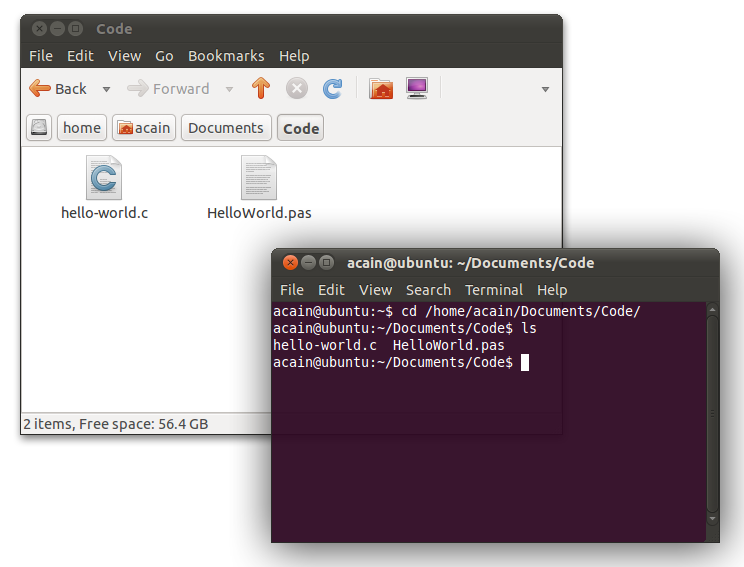
\includegraphics[width=0.9\textwidth]{./topics/programs-and-compilers/images/LinuxFiles} 
   \caption{Changing directories in Linux (Ubuntu)}
   \label{fig:linux-files}
\end{figure}

\begin{figure}[p]
   \centering
   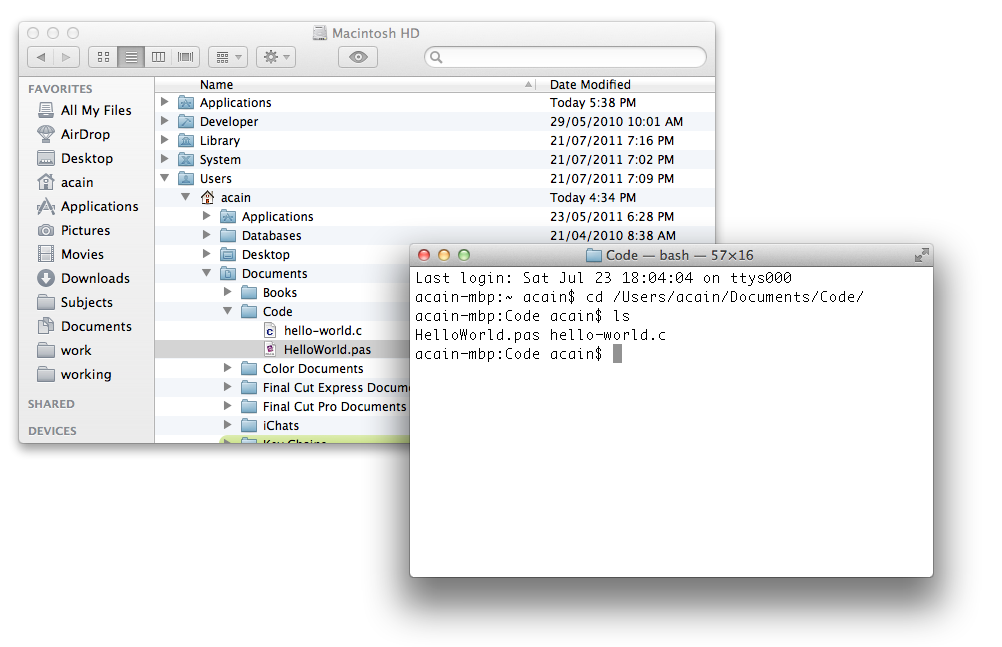
\includegraphics[width=0.9\textwidth]{./topics/programs-and-compilers/images/MacFiles} 
   \caption{Changing directories in MacOS}
   \label{fig:mac-files}
\end{figure}


\begin{figure}[p]
   \centering
   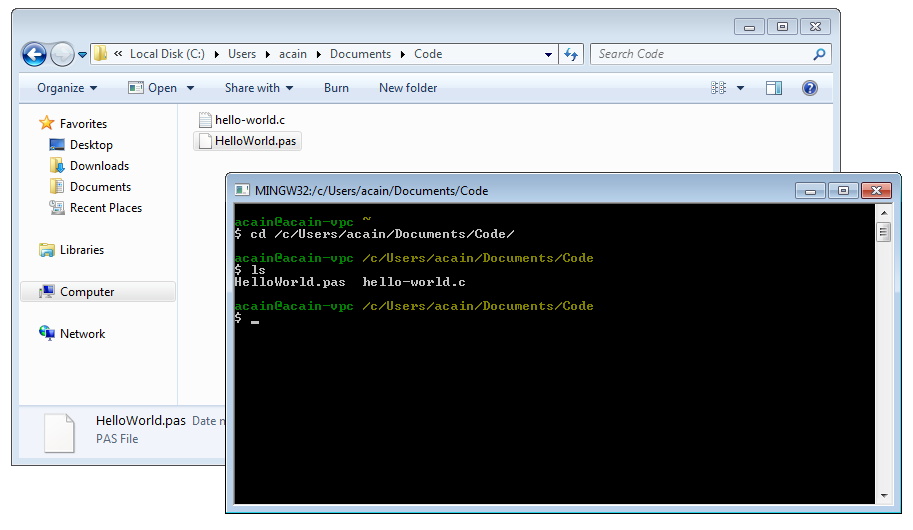
\includegraphics[width=\textwidth]{./topics/programs-and-compilers/images/WindowsFiles} 
   \caption{Changing directories in Windows}
   \label{fig:win-files}
\end{figure}



% subsubsection bash (end)

% subsection terminal (end)
\clearpage
\subsection{The First Program: Hello World} % (fold)
\label{sub:hello world}

There is one very special program that all developers create. This is the first program a software developer creates when they start using a new language, or technology. It is the famous \textbf{Hello World}!

This is a very simple program, it runs and outputs the text `Hello World' to the Terminal. So, why is this the first program? It makes sure that everything is set up correctly. If `Hello World' does not work, then there is something wrong with your setup you need to check.

Listings \ref{lst:hello-world-c} and \ref{lst:hello-world-pas} show the code for the `Hello World' program written with the C++ and Pascal programming languages. Both programs result in the same output when run: they write the text `Hello World!' to the Terminal. They both use the same basic programming structures, and they both go about performing the task in the same way. At this stage, however, they are both just fancy text. What we need to do is use a special tool to convert these into \emph{programs}, we need to \textbf{compile} them.

\csection
{
\ccode{lst:hello-world-c}{Hello World code in C++.}{code/c/program-creation/hello-world.c}
}

\passection{
 \pascode{lst:hello-world-pas}{Hello World code in Pascal.}{./topics/program-creation/pascal/HelloWorld.pas}
}

\mynote{
\begin{itemize}
  \item This source code needs to be written into a \textbf{text file}.
  \item C++ source code usually has a \textbf{.cpp} file extension. For example, \textbf{hello-world.cpp}.
  \item Pascal source code usually has a \textbf{.pas} file extension. For example \textbf{HelloWorld.pas}.
  \item It is a good idea to create a directory (folder) under which you will place your code. Within this directory you can create other directories for individual projects, or for the code related to the chapters in this book.
\end{itemize}
}

% section hello world (end)

\input{topics/programs-and-compilers/concepts/Summary}


% section concepts_related_to_building_programs (end)

% ========================
% = Using these concepts =
% ========================

\clearpage
\section{Using these concepts: Compiling a Program} % (fold)
\label{sec:using_these_concepts_compiling_a_program}

Now that the concepts have been presented, let us have a look at how these can be used to create a program. We will take the code from the Hello World, and use a compiler to turn this code into a program that we can then execute. This process is the same for large and small programs.

\subsection{The SplashKit Manager: skm} % (fold)
\label{sub:skm}

Before we get started, there is one additional tool that we can use to help make SplashKit programs easier to work with: the SplashKit Manager (\textbf{skm}). `skm' is a command line tool that comes with SplashKit when you install it. It is designed to take your compiler instructions, and add the extra options needed to link with the SplashKit library.

The best way to get started with a SplashKit program is to create a new folder (directory) in your file system that will be used to store the code and other files related to that program. 

\csection{
The following commands create a \emph{MyProject} folder, setup a new C++ project, and then compile it into a program.

\bashcode{lst:c-create-project}{Creating a C++ project with skm.}{code/c/program-creation/create-cpp-project.sh}
}

\passection{
The following commands create a \emph{MyProject} folder, setup a new Pascal project, and then compile it into a program.

\bashcode{lst:pas-create-project}{Creating a Pascal project with skm.}{code/pascal/program-creation/create-fpc-project.sh}
}

\subsection{Making the Hello World Program} % (fold)
\label{sub:compiling_code}

\lref{lst:hello-world-c} and \lref{lst:hello-world-pas} show the source code for the Hello World program. To make this into a program you need to:

\begin{enumerate}
  \item Write the code into a text file.
  \item Save the text file to disk.
  \item Compile it.
\end{enumerate}

Step 1 and 2 can be accomplished with any text editor, but the best ones to use highlight your code. Each programming language has rules that determine how its code must be formatted. This is known as the language's \textbf{syntax}. You can get text editors that understand these rules, and highlight your code as you type. This is called \textbf{syntax highlighting}. This highlighting can help you identify any little mistakes you make. 

\fref{fig:cpp-example} shows the Hello World code in Visual Studio Code with C++, which has a consistent look across all platforms. The figure also includes the command line instructions needed to setup a new SplashKit C++ project, and compile it.

\begin{figure}[h]
   \centering
   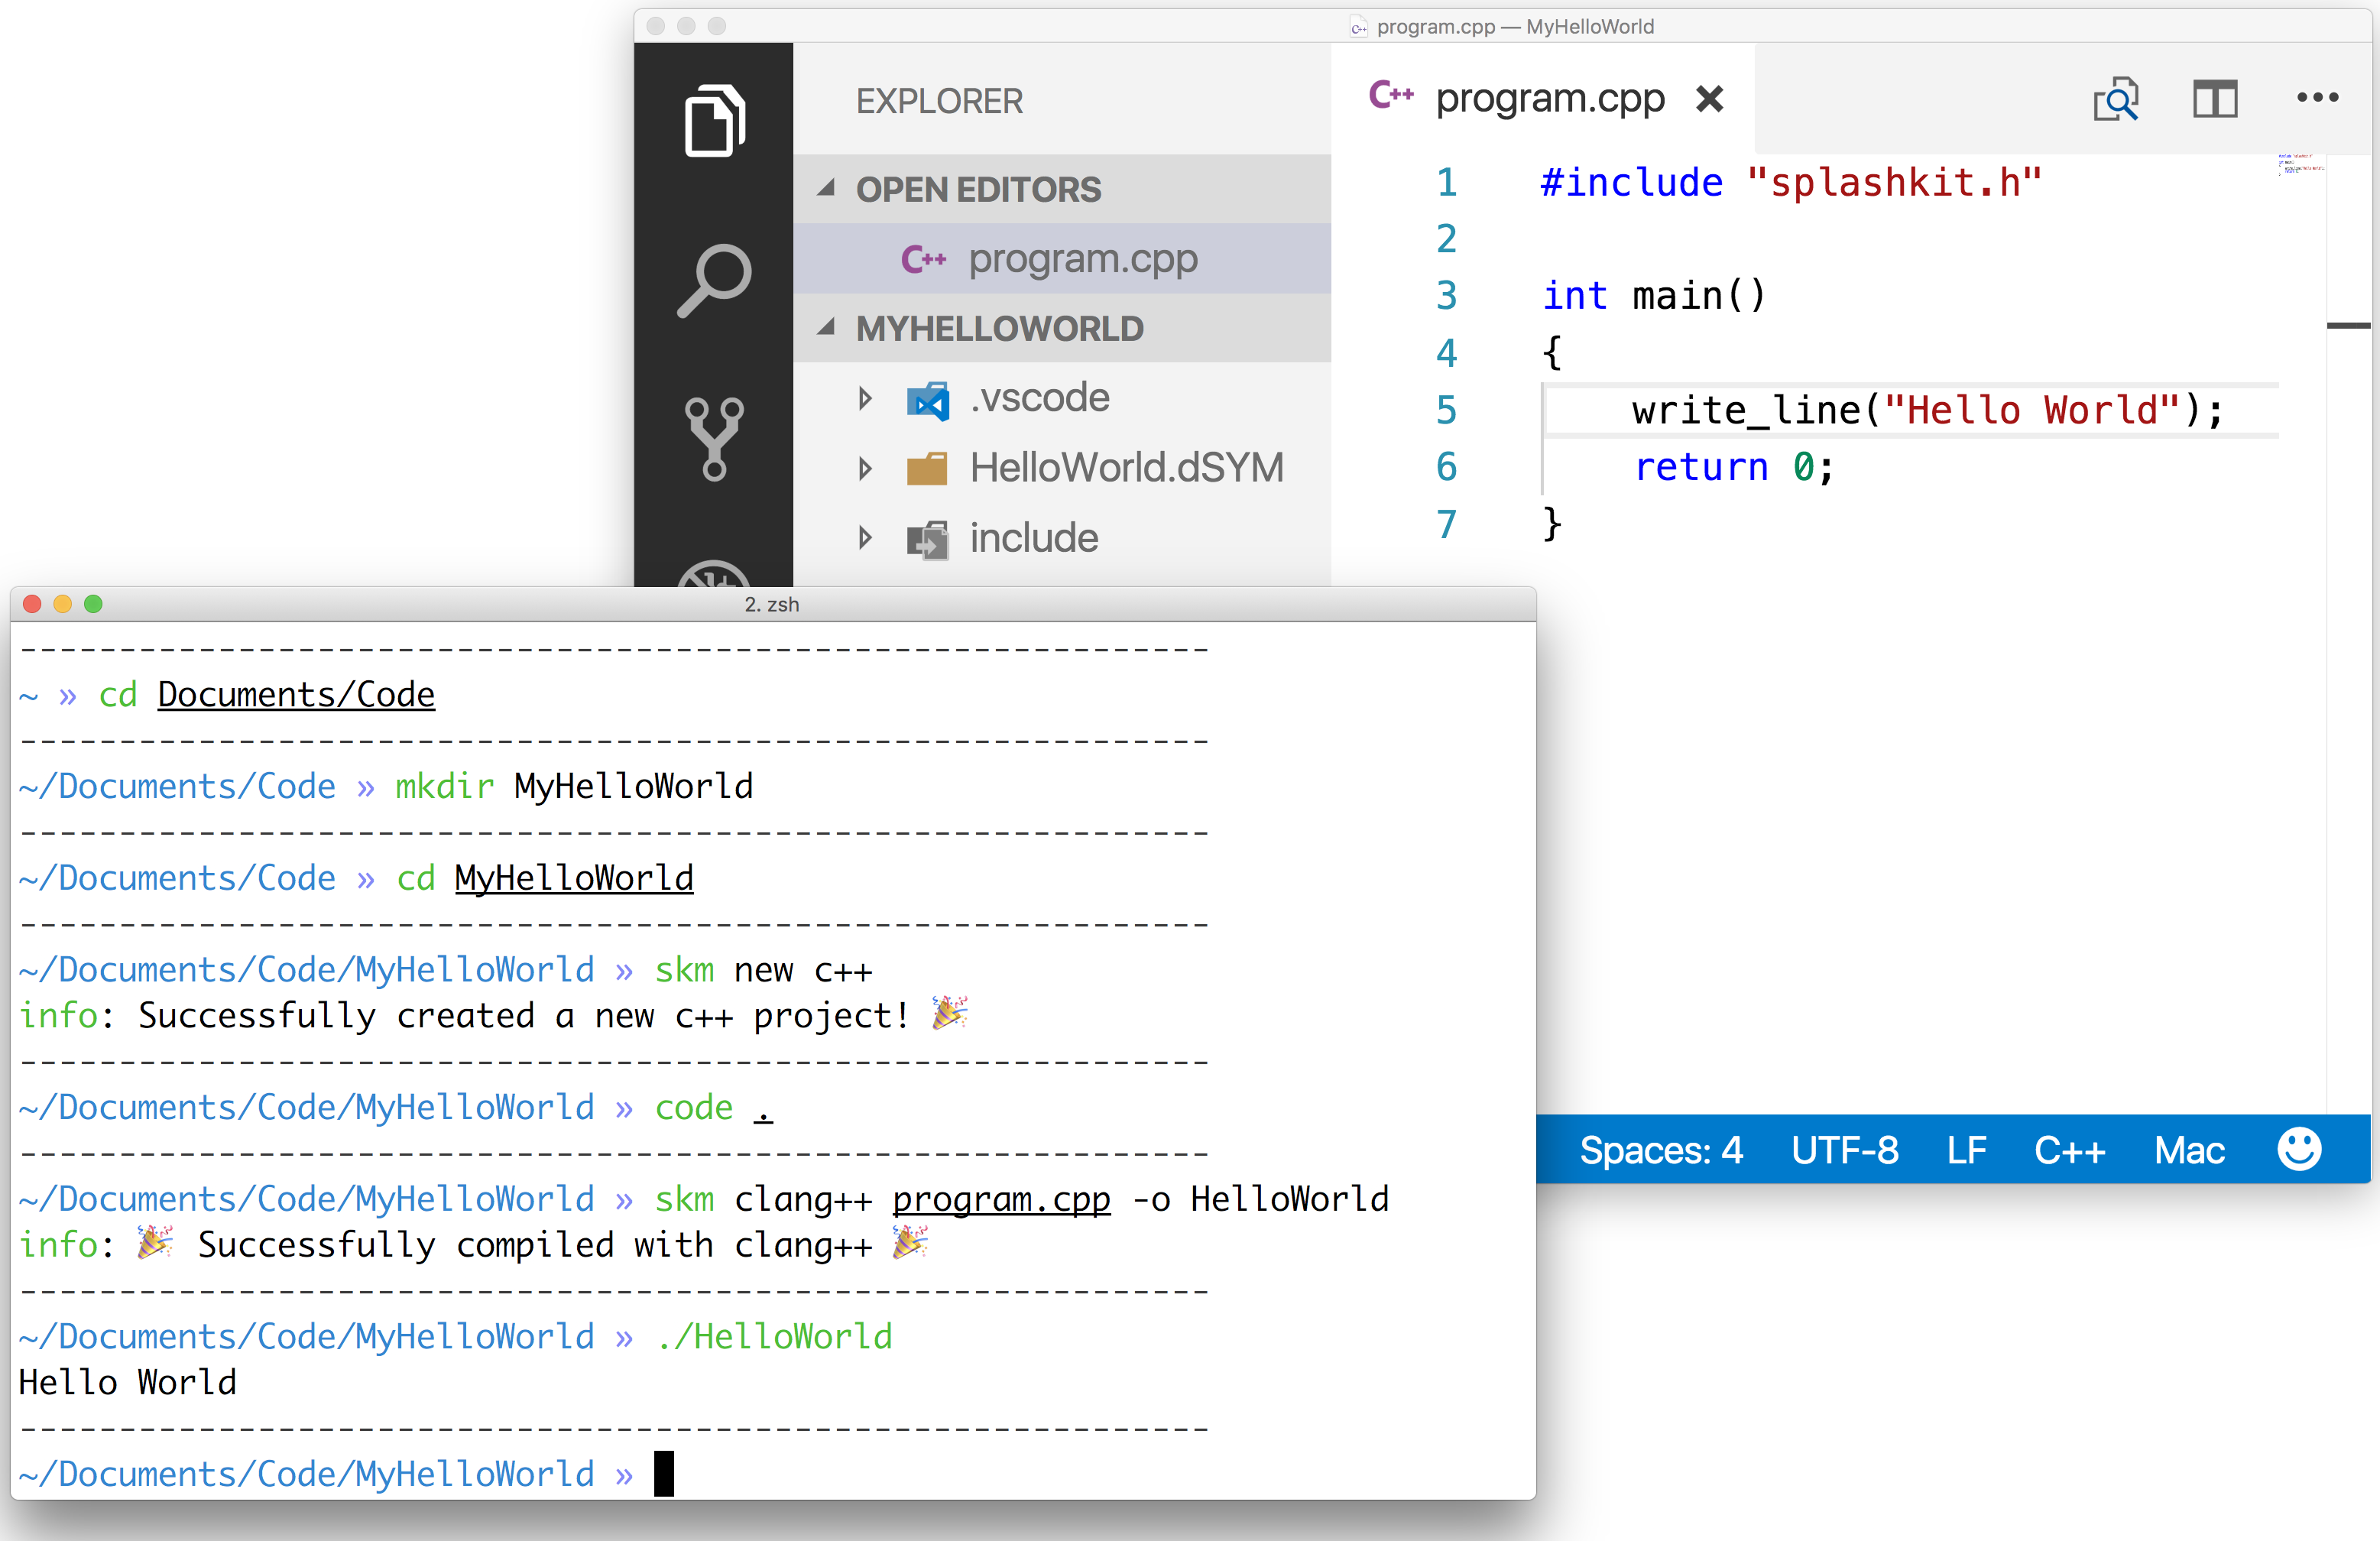
\includegraphics[width=0.8\textwidth]{./topics/programs-and-compilers/images/CppExample} 
   \caption{Editing and Compiling C++ code in Visual Studio Code}
   \label{fig:cpp-example}
\end{figure}

\fref{fig:fpc-example} shows the Hello World code in Visual Studio Code, which has a consistent look across all platforms. The figure also includes the command line instructions needed to setup a new SplashKit Pascal project, and compile it.

\begin{figure}[h]
   \centering
   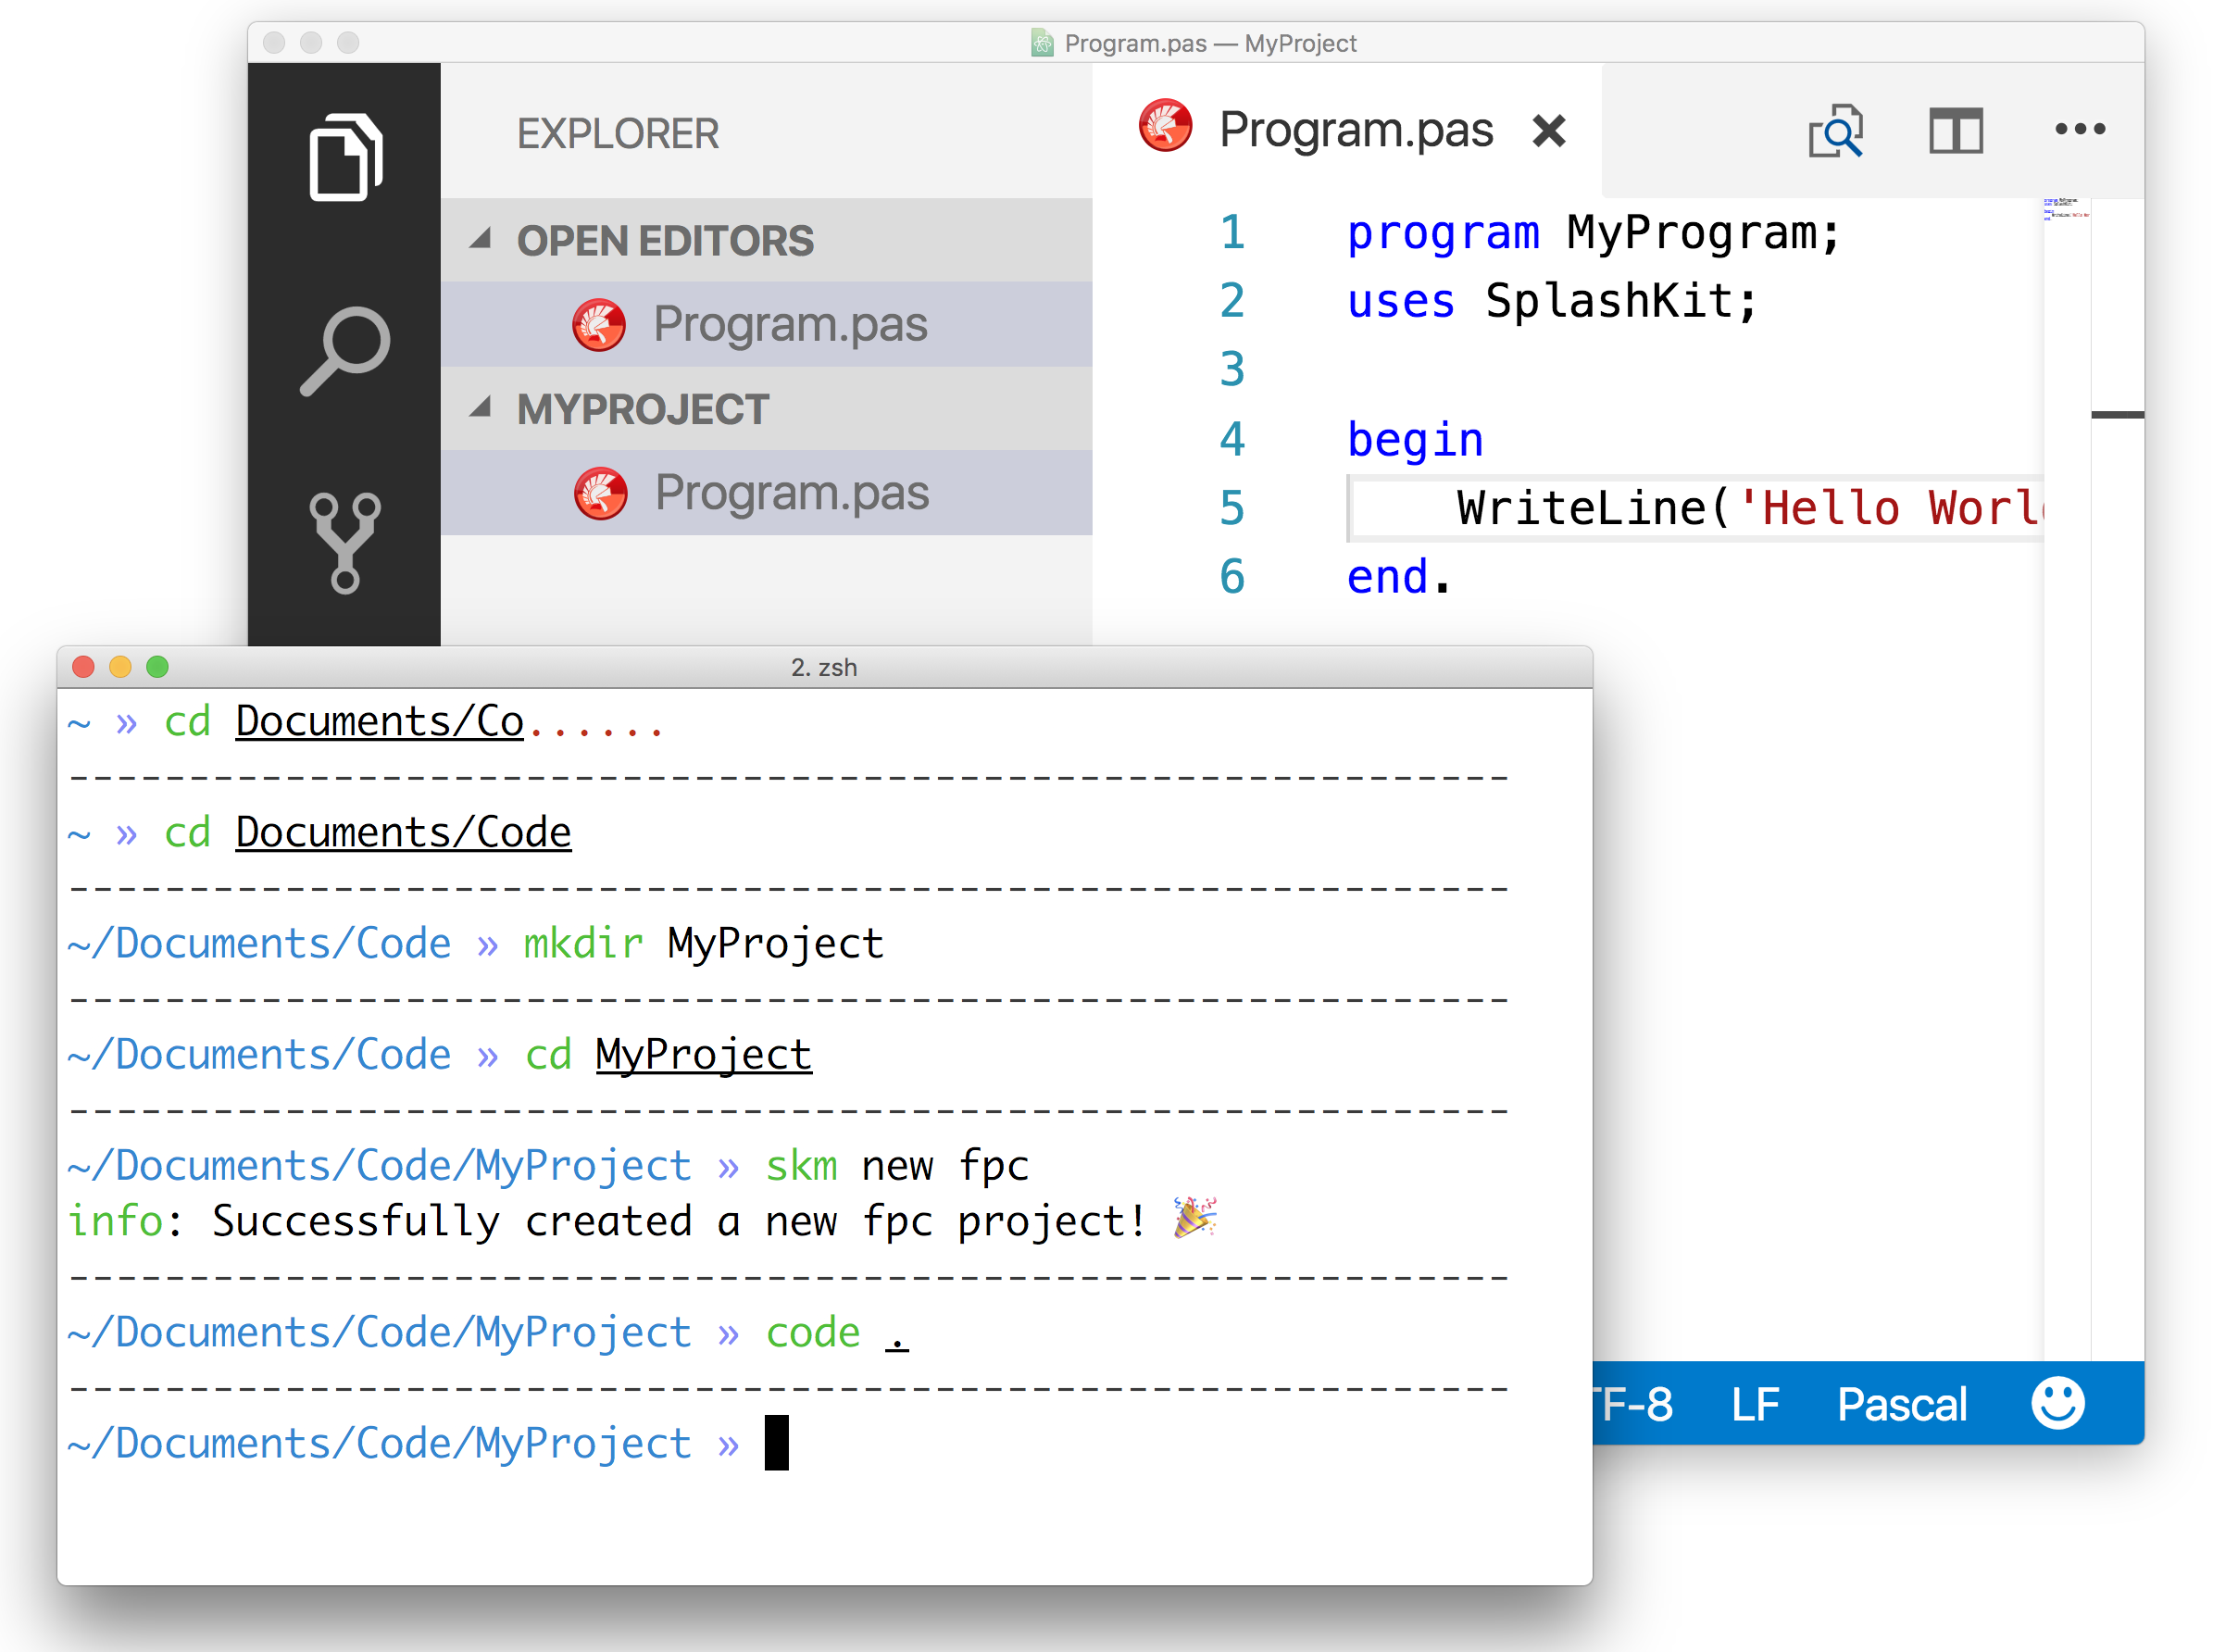
\includegraphics[width=0.8\textwidth]{./topics/programs-and-compilers/images/FpcExample} 
   \caption{Editing and Compiling Pascal code in Visual Studio Code}
   \label{fig:fpc-example}
\end{figure}

\clearpage
\subsubsection{Running the Compiler} % (fold)
\label{ssub:running_the_compiler}

Once you have saved the code to file it is time to compile your program. For this you are going to need to open a \nameref{sub:terminal}, and change into the directory where you saved the source code file. Once you are in this directory it is time to run the compiler.

When you run the compiler you need to give it two kinds of information: options, and the name of the file to compile. The compiler will read the code in the file you give it, and convert this to machine code as shown in \sref{sub:source_code_and_the_compiler} \nameref{sub:source_code_and_the_compiler}. The exact command you use depends on the compiler you are using.

\csection{
In C++ the compiler we will be using is called \textbf{clang++} (or \textbf{g++} the \textbf{GNU C++ Compiler}). The command you need to run in the Terminal is shown in Listing \ref{lst:compile-hello-world-c}. The \emph{-o name} option tells the compiler the name of the program file to create. In our example this will compile the code in \emph{hello-world.cpp} and save the machine code into a program called \emph{HelloWorld}.

\bashcode{lst:compile-hello-world-c}{Compiling C code.}{code/c/program-creation/compile-hello-world.sh}
}

\passection{
In Pascal the compiler we will be using is called \textbf{fpc}, which stands for the \textbf{Free Pascal Compiler}. The command you need to run in the Terminal is shown in Listing \ref{lst:compile-hello-world-pas}. The \emph{-S2} option is used to tell fpc to compile using the latest `Free Pascal' version of the language. In our example this will compile the code in \emph{HelloWorld.pas} and save the machine code into a program called \emph{HelloWorld}, which it gets from the name of the Pascal file.

\bashcode{lst:compile-hello-world-pas}{Compiling Pascal code.}{code/pascal/program-creation/compile-hello-world.sh}
}

Once you get the program to compile you can run it! This will load your program into memory, and start its steps running. The HelloWorld program will output the text `\texttt{Hello World!}' to the Terminal. To run the program you need to use its name. The command you need to enter is shown in \lref{lst:run-hello-world}, and in \fref{fig:run-helloworld}. The \texttt{./} before the file tells Bash to look in the current directory for the program.

\bashcode{lst:run-hello-world}{Bash command to run HelloWorld}{topics/programs-and-compilers/run-hello-world.sh}

\begin{figure}[h]
   \centering
   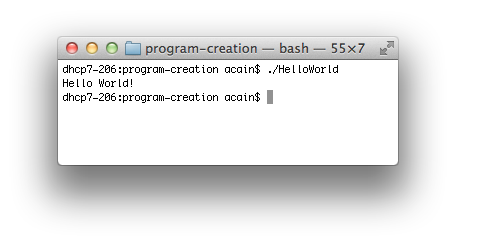
\includegraphics[width=0.7\textwidth]{./topics/programs-and-compilers/images/HelloWorld} 
   \caption[Hello World Terminal]{Hello World run from the Terminal}
   \label{fig:run-helloworld}
\end{figure}

% subsubsection running_the_compiler (end)

\subsubsection{When things do not work} % (fold)
\label{ssub:when_things_do_not_work}

Compilers are very specific about the code you give it. If the source code you try to compile does not follow all of the rules of the language then the compiler will fail, and end with an error message. These errors, called \textbf{syntax errors}, could be as small as missing a semicolon (;), or misspelling a name. To get your program to compile you will need to correct any syntax errors the compiler finds in your code.

\begin{figure}[h]
   \centering
   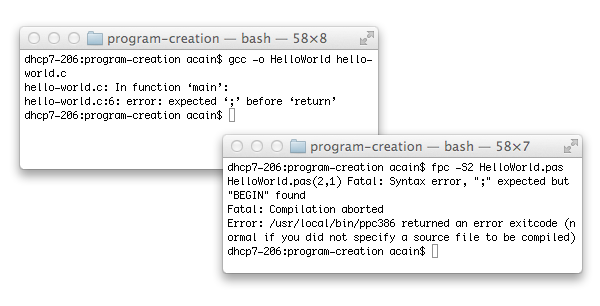
\includegraphics[width=0.8\textwidth]{./topics/programs-and-compilers/images/SyntaxErrors} 
   \caption{These Terminals show some syntax errors from programs that are missing a single semicolon (;)}
   \label{fig:syntax-errors}
\end{figure}

\fref{fig:syntax-errors} shows an example output caused by removing a single semicolon from the Hello World program's code. The numbers in the error messages give you an idea of where the compiler got to when it encountered the error. So the text \texttt{hello-world.c:6:} output from the C compiler indicates that the compiler got to line 6 before it encountered the error. The text \texttt{HelloWorld.pas(2,1)} output from the Pascal compiler indicates that it got up to line 2 character 1 before it encountered the error.

When the compiler encounters these issues it does not create the executable program. You need to learn to use these error messages to help you locate errors in your code, so that you can fix them, and then run the compiler again to generate your program.

\mynote{
\begin{itemize}
  \item Syntax errors are very common. Do not worry when this occurs to you.
  \item Always start with the first error. The compiler will try to continue compiling your code after it finds an error. This can mean that later errors do not really exist, once you fix the earlier ones.
  \item Unfortunately compiler error messages are not always very clear on what the cause of the error is. You need to learn how to read and understand these messages.
  \item To get good at programming requires lots of practice.
\end{itemize}
}

% subsubsection when_things_do_not_work (end)



% section the_compiler (end)


% section using_these_concepts_compiling_a_program (end)

% =============
% = C Section =
% =============
\clearpage
\def\pageLang{c}
\section{Building Programs in C} % (fold)
\label{sec:building_programs_in_c}

\clearpage
\subsection{Hello World in C} % (fold)
\label{sub:hello_world_in_c}

Now that you have the compiler installed you can create your first program: the famous \textbf{Hello World} discussed in \sref{sub:hello world}. The C code for this is shown in \lref{lst:hello-world-c-c}. This code tells the computer to `print' the text \emph{Hello World!} to the Terminal. Do the following to create this program for yourself, see the notes below for hints:

\begin{enumerate}
  \item Open your text editor
  \item Create a new text file
  \item Type\footnote{Do not just copy and paste it out of the text, type it in yourself as this will help you learn the concepts being covered.} in the text below, making sure you get every character correct.
  \item Save your program's code in a file called \textbf{hello-world.c}, and note the directory where it is saved
  \item Open the Terminal
  \item Change into the directory where you save the file
  \item Compile the program using \texttt{gcc -o HelloWorld hello-world.c}
  \item Run the program using \texttt{./HelloWorld}
\end{enumerate}

Well done, you have now created and run your first C program!

\csection
{
\ccode{lst:hello-world-c-c}{Hello World code in C.}{code/c/program-creation/hello-world.c}
}

\mynote{
\begin{itemize}
  \item See \sref{sec:installing_a_text_editor} \nameref{sec:installing_a_text_editor} for details on installing the Text Editor.
  \item See \nameref{ssub:bash} in \sref{sub:terminal} for an example of how to use the Terminal.
  \item See \sref{sec:using_these_concepts_compiling_a_program} \nameref{sec:using_these_concepts_compiling_a_program} for the overall process and the output you should expect from the program.
\end{itemize}
}

% subsection hello_world_in_c (end)
\clearpage
\subsection{Installing GCC} % (fold)
\label{sub:installing_gcc}

You can get the gcc compiler for Linux, Mac OS, and Windows. The following section describe where it is you can find these programs, and how to install them.

\subsubsection{Installing gcc on Linux} % (fold)
\label{ssub:linux}

It should be relatively easy to install \textbf{gcc} for Linux. If gcc is not already installed on your machine you should check with the Linux distribution on how to install the build tools. To install this on Ubuntu linux use the command shown in \lref{lst:apt-get-gcc}.

\bashcode{lst:apt-get-gcc}{The command line instruction to install gcc on Ubuntu}{topics/programs-and-compilers/c/apt-get-gcc.txt}

% subsubsection linux (end)

\subsubsection{Installing gcc on Mac OS} % (fold)
\label{ssub:installing_gcc_on_mac_os}

To install \textbf{gcc} on Mac OS you need to install the \textbf{XCode} developer tools. You can get the latest version of XCode from the \textbf{Mac App Store} (yes it is free).

XCode links:
\begin{itemize}
  \item Apple's XCode website \url{http://developer.apple.com/xcode/}
  \item XCode in the Mac App Store  \url{http://itunes.apple.com/au/app/xcode/id448457090?mt=12}
\end{itemize}


% subsubsection installing_gcc_on_mac_os (end)

\subsubsection{Installing gcc on Windows} % (fold)
\label{ssub:installing_gcc_on_windows}

To get \textbf{gcc} on Windows you need to install the \textbf{MinGW} program. This includes the MinGW Shell, the Terminal equivalent for Windows. Read the Getting Started page from the links below, and follow the steps for the \textbf{Graphical User Interface Installer}. When following the installer make sure that you choose to install the MinGW Shell as well as the C compiler.

\begin{itemize}
  \item The project's Website \url{www.mingw.org}
  \item Instructions for installing MinGW: \url{http://www.mingw.org/wiki/Getting_Started}
  \item Follow the link from the Getting Started article, or download MinGW from Source Forge at \url{http://sourceforge.net/projects/mingw/}
  \item It is a good idea to restart after installing MinGW to make sure all its settings are applied.
\end{itemize}

% subsubsection installing_gcc_on_windows (end)
\clearpage
\subsubsection{Testing gcc has installed} % (fold)
\label{ssub:testing_your_install}

To test that you have successfully installed gcc you can do the following:
\begin{enumerate}
  \item Open a Terminal window. (See the notes on the \nameref{sub:terminal} page for the location of the Terminal program)
  \item At the terminal type \textbf{\texttt{gcc}}. You should see something similar to \fref{fig:gcc-install}. If you see the message `\texttt{-bash: gcc: command not found}' this means the install has not worked correctly. Please review the install steps for your Operating System or get someone to check your install.
\end{enumerate}

\begin{figure}[h]
   \centering
   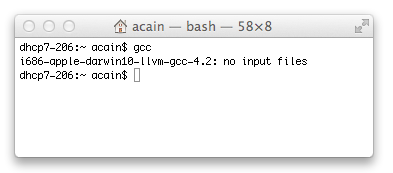
\includegraphics[width=0.5\textwidth]{./topics/programs-and-compilers/images/gccInstall} 
   \caption{Testing gcc has been installed}
   \label{fig:gcc-install}
\end{figure}

Once you have got this working you can move on to installing a text editor.


% subsection testing_your_install (end)

% subsection installing_gcc (end)
\clearpage
\subsection{Installing a Text Editor} % (fold)
\label{sub:installing_a_text_editor}

When you are programming you will spend most of your time in a Text Editor. The best kinds of editors for program code include syntax highlighting where the editor uses details about the language to highlight parts of the code as you write it. This can make it easier to find and fix small errors as you go.

\subsubsection{gEdit on Linux} % (fold)
\label{ssub:gedit_on_linux}

The \textbf{gEdit} program is a syntax highlighting text editor for Linux. In Ubuntu this is the standard \textbf{Text Editor} program found in \emph{Accessories}. This should already be installed. Another good text editors is \texttt{Kate}.

% subsubsection gedit_on_linux (end)

\subsubsection{TextWrangler Mac OS} % (fold)
\label{ssub:textwrangler_or_textmate_on_mac_os}

TextWrangler is a free syntax highlighting text editor for Mac OS. You can download and install this from the \textbf{Mac App Store}, or from their web site.

\begin{itemize}
  \item Mac App Store link: \url{http://itunes.apple.com/au/app/textwrangler/id404010395?mt=12}
  \item Website: \url{http://www.barebones.com/products/textwrangler/}
  \item TextMate is another good editor, though it is not free: \url{http://macromates.com/}
\end{itemize}

% subsubsection textwrangler_or_textmate_on_mac_os (end)

\subsubsection{Notepad++ for Windows} % (fold)
\label{ssub:notepad_for_windows}

Notepad++ is a free syntax highlighting text editor for Windows. You can download and install this from the Notepad++ website.

\begin{itemize}
  \item Notepad++: \url{http://notepad-plus-plus.org/}
\end{itemize}

% subsubsection notepad_for_windows (end)

% subsection installing_a_text_editor (end)
\clearpage
\subsection{Graphical Applications with SwinGame} % (fold)
\label{sub:graphical_applications_with_swingame}

SwinGame is a 2D game creation library. It contains a number of resources that you can use to create small games using the C programming language. To get started with SwinGame you need to download a \emph{template} from the website. The template includes everything you need to get started creating a game in SwinGame.

\subsubsection{Coding a SwinGame} % (fold)
\label{ssub:coding_a_swingame}

The code for your SwinGame can be found in the \textbf{\texttt{src}} folder. This includes a \texttt{\textbf{GameMain.c}} file, where you can place your source code.

% subsubsection coding_a_swingame (end)

\subsubsection{Compiling a SwinGame} % (fold)
\label{ssub:compiling_a_swingame}

There are a number of steps that you need to follow to compile a SwinGame. Fortunately, all of these are written for you in the script called \textbf{\texttt{build.sh}}. This script to included in the project template. 

% subsubsection compiling_a_swingame (end)

\subsubsection{Running a SwinGame} % (fold)
\label{ssub:running_a_swingame}

% subsubsection running_a_swingame (end)

% subsection graphical_applications_with_swingame (end)

% section building_programs_in_c (end)

% ===================================
% = Understanding Building Programs =
% ===================================

\clearpage
\def\pageLang{}
\section{Understanding Program Compilation} % (fold)
\label{sec:understanding_program_compilation}

An in depth look at how programs and compilers work is beyond the scope of this book. Instead, this chapter focuses on two aspects that can help you understand why we need compilers, and how these are able to help us. These topics are \nameref{sub:levels_of_abstraction}, followed by \nameref{sub:computers_and_intelligent_behaviour}.

\subsection{Levels of Abstraction} % (fold)
\label{sub:levels_of_abstraction}

Programs are very complicated. Trying to keep all of the details about how it works in focus all of the time would take a large amount of effort, and slow you down. As humans we have developed strategies for dealing with these kinds of situations. What we do is create \emph{layers} of abstraction.

A layer, or level, of abstraction provides a means of managing details at a similar level of detail. This means that all aspects of that level are similar, and related to each other. When you are working at a certain level, you think in terms of the tools and artefacts that are available to you. 

These levels build on top of each other, with each layer being built on top of the lower layer, and providing the foundation for the next higher layer. Within a layer of abstraction you do not need to think about the lower levels of abstraction, most of the time. However, it is always good to know the details of at least one level of abstraction below the level you are working at.

\subsubsection{Programming Abstraction Levels} % (fold)
\label{ssub:programming_abstraction_levels}

Computers are unintelligent. This is one of the first, and most important, things you need to understand when starting to create your own programs. A computer is a machine that can be programmed using \nameref{sub:machine_code}. These binary commands instruct the computer to perform basic actions such as adding numbers, reading values from memory, storing values in memory, jumping to new instructions elsewhere in memory, and other simple tasks. While this is a very low level, it is not the lowest level of abstraction.

Below machine code, there is the abstraction for \textbf{binary}. This is the idea that you can have a number system based on two digits, 0 and 1. The machine code level builds on this idea, creating a set of instructions that can be used to tell the computer what to do. Below binary there is the concept of \textbf{gates}, which are themselves built on top of \textbf{electronic circuits}, which in turn are made from \textbf{discrete electronic components}. Even these low level electronic components are based upon something else, but to discuss this we would need to delve into the realm of \textbf{semiconductors} and \textbf{Quantum Mechanics}. From machine code you can also work up to \nameref{sub:assembly}, and then to \nameref{sub:source_code_and_the_compiler}.

Whenever you are working on something you need to be able to work at that level of abstraction, and have an understanding of the level below, and the level above. For programming this means that you will need to understand of the tools provided to you by the language (a level below), and you need to understand the features and functions of the program you are creating (a level above).

In this book the \emph{Understanding} section of each chapter will help you see how the concepts covered work at a lower level of abstraction. Often this means these sections are very detailed. You should read these sections to understand how the abstractions (concepts) covered in the chapter work, at a level of abstraction lower than you will be working at.

% subsubsection programming_abstraction_levels (end)
% subsection levels_of_abstraction (end)
\clearpage
\subsection{Computers and Intelligent Behaviour} % (fold)
\label{sub:computers_and_intelligent_behaviour}

If computers are unintelligent, how can they do the awesome things they do?

That is a good question. Computers are unintelligent, but programs are not. The computer does not \emph{know} what it is doing. It is following a set of steps that was coded into the program being executed. These steps, however, were created by people, software developers. When a computer does something cool, its because a person told it to do that.

This is why it can be really great fun to be a software developer. You get to make computers do things you want them to. This creativity can be really exhilarating when you finally get your program to do exactly what you want.

\begin{figure}[h]
   \centering
   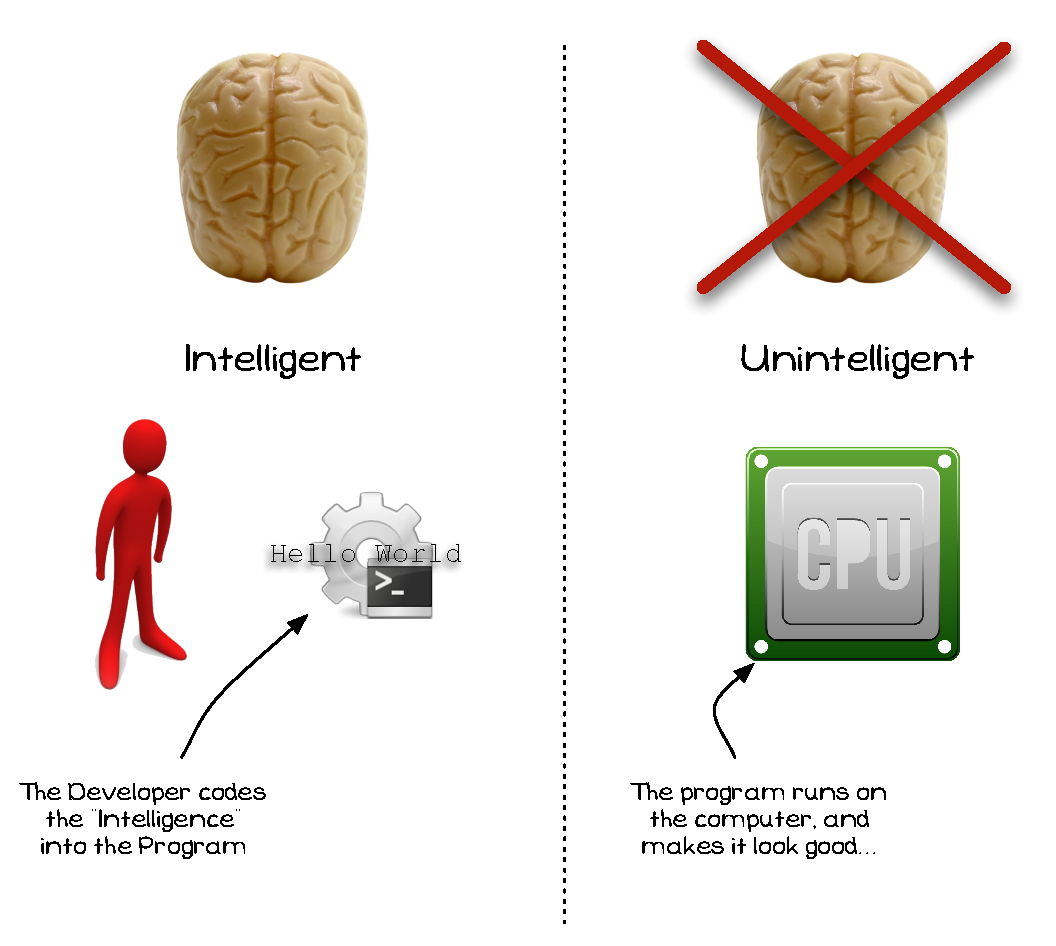
\includegraphics[width=\textwidth]{./topics/programs-and-compilers/diagrams/ProgramIntelligence} 
   \caption{Computers are unintelligent, any interesting behaviour comes from programs created by software developers}
   \label{fig:program-intelligence}
\end{figure}
% subsection computers_and_intelligent_behaviour (end)
% section understanding_ (end)

% ============
% = Examples =
% ============

\clearpage
\section{Exercises on Building Programs} % (fold)
\label{sec:examples_and_exercises_on_building_programs}

Read over the concepts in this chapter and answer the following questions:
\begin{enumerate}
  \item What is a \nameref{sub:what_is_a_program_}? What does it contain?
  \item What is \nameref{sub:machine_code}?
  \item Can you write programs in Machine Code? Explain any issues associated with this.
  \item What is \nameref{sub:assembly}?
  \item Can you write programs in Assembly? Explain any issues associated with this.
  \item What tool is used to convert Assembly to Machine Code?
  \item What is Source Code?
  \item What are the advantages of programming at a Source Code level?
  \item What tool is used to convert Source Code to Machine Code?
  \item Why do you need to convert Source Code and Assembly to Machine Code?
  \item What is the \nameref{sub:terminal}? 
  \item What is Bash?
  \item Which command is used to change directories in Bash?
  \item With Bash, how can you check which directory is the current working directory?
  \item How can you list all of the files in the current directory?
  \item Why program `Hello World'? What does it do for you?
  \item What is the name of the C or Pascal compiler we will be using in this book?
  \item How intelligent is your computer?
\end{enumerate}

\bigskip
Apply what you have learnt to the following tasks:

\begin{enumerate}
  \item Enter the code, compile, and run the `Hello World' program.
  \item Try changing the code to output a different message. After you have made the changes you will need to re-compile and run the program.
\end{enumerate}

\bigskip
If you want to further your knowledge in this area you can try to answer the following questions. The answers to these questions will require you to think harder, and possibly look at other sources of information.
\begin{enumerate}
  \item What is the difference between a compiler and an interpreter? How are programs of interpreted languages, such as Python, executed?
  \item If you compile a program for an Intel CPU on UNIX, can you run this on a UNIX machine that has a PowerPC CPU?
  \item If you compile a program on a Windows machine can you run the resulting program on a UNIX machine with the same CPU architecture?
  \item What is a fat, or Universal, binary?
  \item What is a Virtual Machine?
\end{enumerate}

% section examples_and_exercises_on_building_programs (end)


% chapter building_programs (end)
  \chapter{Program Creation} % (fold)
\label{cha:program_creation}

\begin{quote}
  \Fontlukas\Large
  \renewcommand{\LettrineTextFont}{\relax}
  \lettrine[image=true,lines=3,lraise=0.1]
  {C}{asting} spells crafted by others is alright, but the true power of magic can only be realised by crafting your own spells. You have done well mastering the tools, so now let us turn our attention to the study of the arcane knowledge of spell craft. To create your own spells you need to know\ldots
\end{quote}

\bigskip

Compiling programs crafted by others is alright, but the true power of programming can only be realised by learning to craft your own programs. \cref{cha:building programs} introduced you to the tools you need to compile programs from source code, so now we can turn our attention to the study program creation.

This chapter introduces the artefacts used to create programs, and how you can code these using a programming language. You will start by learning to create simple programs that output information to the Terminal.

When you have understood the material in this chapter you will be able to write the code needed to declare a program, convert this code into an executable program using a compiler, and then run the program you created. You will have made those first important steps in your journey to master this arcane knowledge. 

\minitoc

% ============
% = Concepts =
% ============
\clearpage
\section{Program Creation Concepts} % (fold)
\label{sec:program_creation_concepts}

Our first program is going to display some text to the Terminal. In this section you will be introduced to the programming artefacts and terminology you will need to use to create this program. This first step is important and will require you to have installed a C or Pascal compiler, see \cref{cha:building programs} for instructions.

A programming \textbf{artefact} is something that can be created and used within your code. In this chapter we will look at creating Programs, and using a number of other artefacts. The following artefacts will be covered in this chapter:
\begin{itemize}
  \item \nameref{sub:program}: You declare a Program to get the compiler to write a file that can be executed.
  \item \nameref{sub:procedure}: You can call Procedures to perform actions within the program.
  \item \nameref{sec:program-creation-library}: The program can use code from other Libraries. These libraries contain reusable Procedures and Types. 
  \item \nameref{sub:type}: A Type defines how data is interpreted by the program. The language will support a number of basic types by default, and Libraries can add other types. 
\end{itemize}

In addition to these artefacts, you will need to understand some programming \textbf{terminology}. The following terms are discussed in this section:
\begin{itemize}
  \item \nameref{sec:program-creation-statement}: An \textbf{instruction} within the Program.
  \item \nameref{sub:expression}: A \textbf{value} used in a Statement.
  \item \nameref{sub:identifier}: The \textbf{name} of an artefact.
  % \item Literal: A part of an \textbf{expression} where the value is entered directly into the code.
\end{itemize}

This section also introduces the following kinds of instructions. You can use these to get the computer to perform certain \textbf{actions} within your program.
\begin{itemize}
  \item \nameref{sub:procedure call}: The instruction to run a Procedure.
\end{itemize}

We can then use these concepts, artefacts, and instructions to create a Program that includes a call to a procedure that will write some text to the Terminal as shown in Figure \ref{fig:program-creation-helloworld}.

\begin{figure}[h]
   \centering
   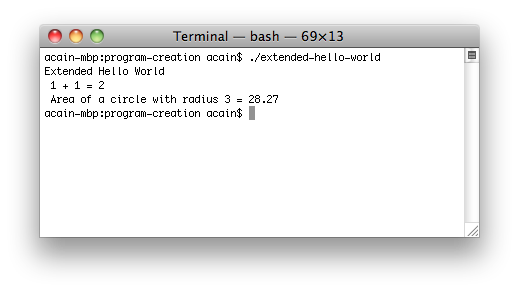
\includegraphics[width=0.8\textwidth]{./topics/program-creation/images/HelloWorld} 
   \caption[Hello World Terminal]{Hello World run from the Terminal}
   \label{fig:program-creation-helloworld}
\end{figure}

\clearpage
\subsection{Program} % (fold)
\label{sub:program}

A program contains the instructions the computer will follow when that program is executed. In your source code you can declare a program in which you code the steps you want followed when your program is executed. When you compile this code the compiler will create an executable file (a \emph{program}) that the user can run. Running the program will then get the computer to perform the steps you wrote in the code.

\begin{figure}[h]
   \centering
   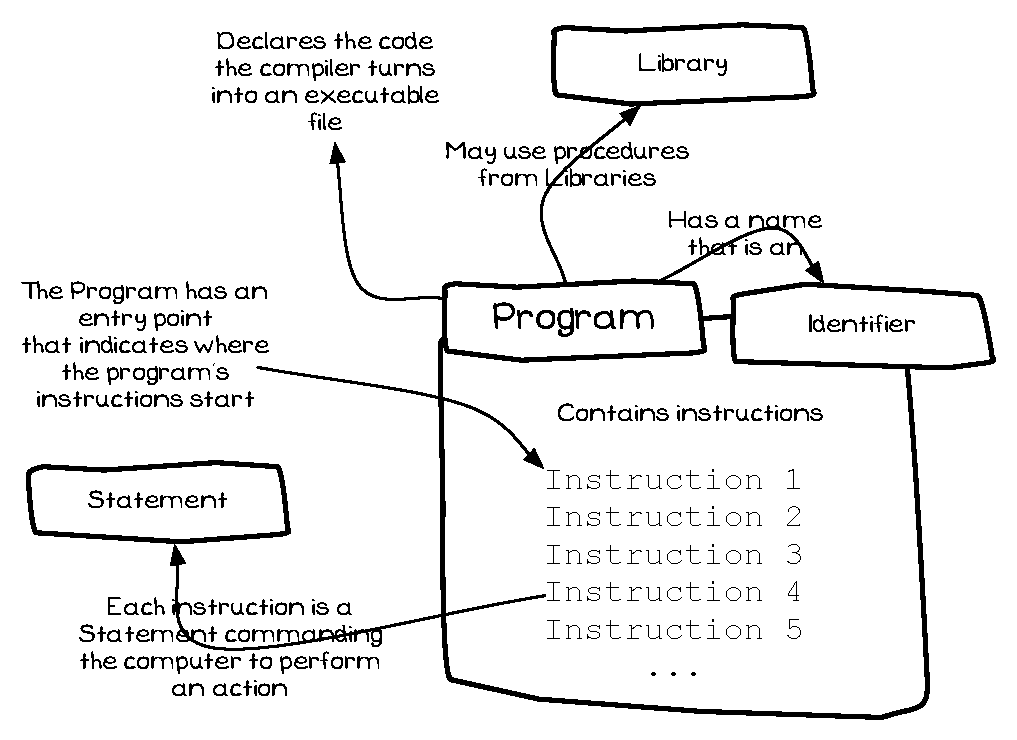
\includegraphics[width=\textwidth]{./topics/program-creation/diagrams/BasicProgramConcept} 
   \caption{A program contains instructions that command the computer to perform actions}
   \label{fig:program-creation-program}
\end{figure}


\mynote{
\begin{itemize}
  \item A program is an \textbf{artefact}, something you can create in your code.
  \item Figure \ref{fig:program-creation-program} shows the concepts related to programs.
  \item A program is a programming artefact used to define the steps to perform when the program is run.
  \item You use the compiler to convert the program's source code into an executable file.
  \item By declaring a program in your code you are telling the compiler to create a file the user can run.
  \item The program has an \textbf{entry point} that indicates where the program's instructions start.
  \item The name of the program determines the name of the executable file.
  \item Your program can use code from a \nameref{sub:library} or number of libraries.
  \item In programming terminology, an instruction is called a \nameref{sub:statement}.
\end{itemize}
}

% section program (end)
\clearpage
\subsection{Statement} % (fold)
\label{sub:statement}

A statement is an instruction for the computer to perform an action, a command telling it what to do. Each \nameref{sub:program} contains a list of statements (commands). When the program is run the computer follows these commands one at a time, in sequence, starting at the program's entry point and ending when it completes the program's last statement.

\begin{figure}[h]
   \centering
   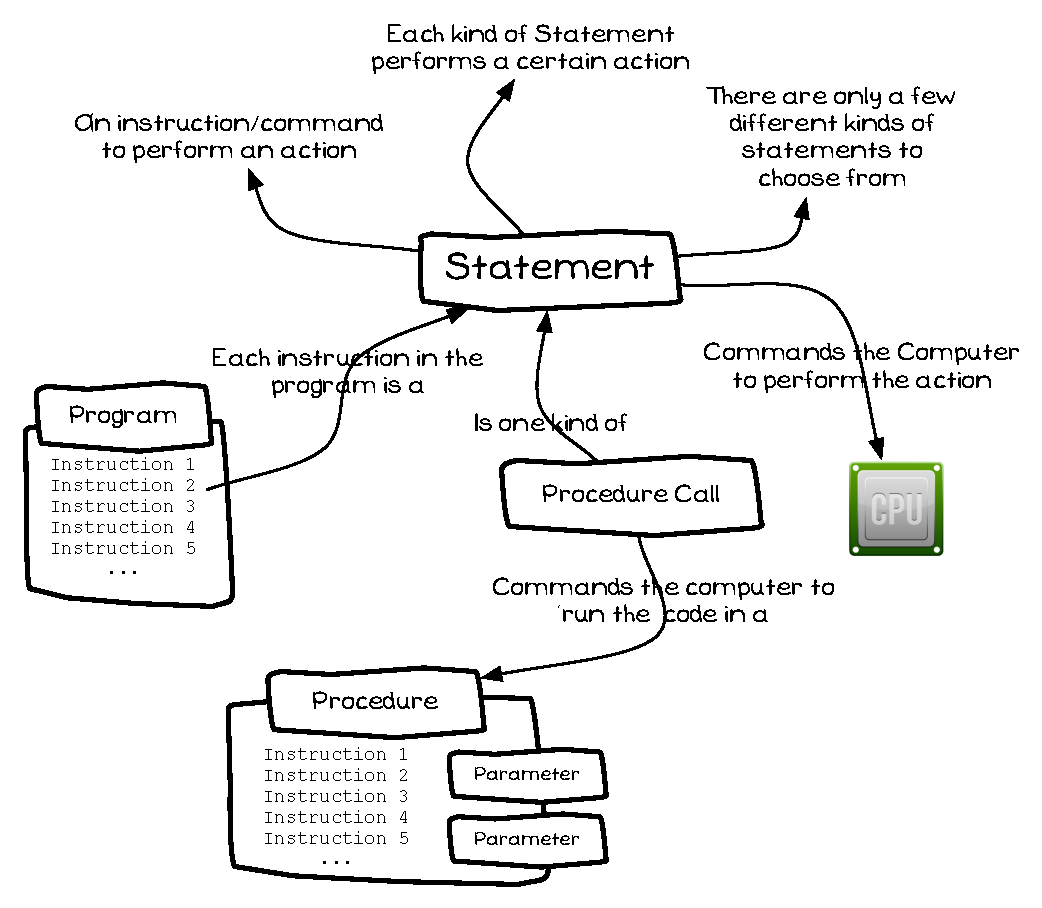
\includegraphics[width=\textwidth]{./topics/program-creation/diagrams/Statement} 
   \caption{A statement is a command for the computer to perform an action}
   \label{fig:program-creation-statement}
\end{figure}


\mynote{
\begin{itemize}
  \item A statement is a \textbf{term} used to describe the instructions in your code.
  \item Figure \ref{fig:program-creation-statement} shows the concepts related to statements.
  \item A statement is a \textbf{command}, an instruction to perform a task.
  \item A \nameref{sub:program} has a list of statements that are followed when it is executed.
  \item There are only a few different kinds of statement.
  \item A \nameref{sub:procedure call} is a kind of statement, it tells the computer to run the code in a \nameref{sub:procedure}.
  \item This style of programming is known as \textbf{Imperative} programming. Imperative means to give authoritative commands, and that is what we do in our programs. Our programs are lists of authoritative commands telling the computer to perform actions.
\end{itemize}
}

% section statement (end)
\clearpage
\subsection{Procedure Call} % (fold)
\label{sub:procedure call}

A procedure call is a kind of \nameref{sub:statement} that instructs the computer to run the code in a \nameref{sub:procedure}. If the procedure requires some data to work with, then this data is passed to the procedure as part of the procedure call. The procedure's name is used to identify the procedure to call.

\begin{figure}[h]
   \centering
   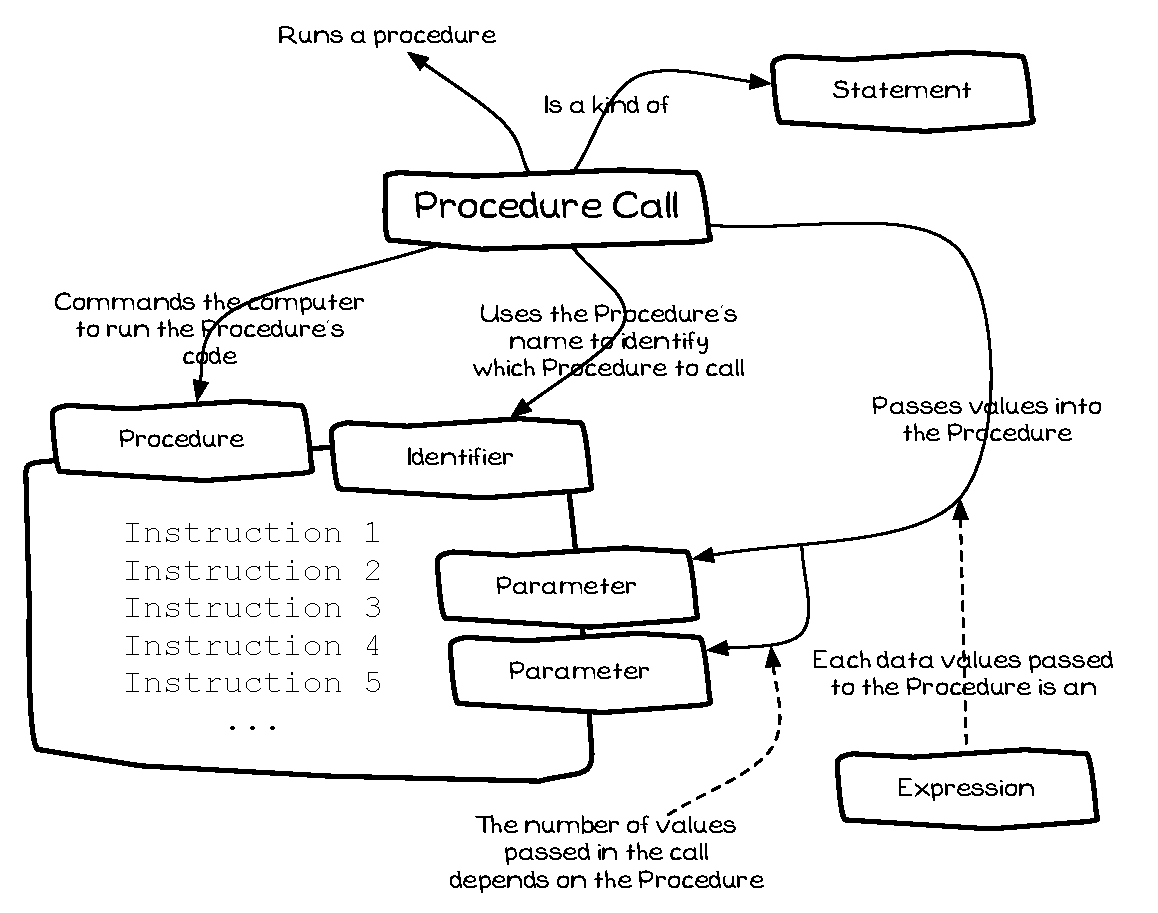
\includegraphics[width=\textwidth]{./topics/program-creation/diagrams/ProcedureCall} 
   \caption{A procedure calls runs a procedure, passing in values for the procedure to use}
   \label{fig:program-creation-procedure call}
\end{figure}


\mynote{
\begin{itemize}
  \item A procedure call is an \textbf{action}, you can call procedures in your code.
  \item Figure \ref{fig:program-creation-procedure call} shows the concepts related to the procedure call.
  \item A procedure call is an instruction to execute a procedure.
  \item You can code a procedure anywhere you can code a statement.
  \item The \nameref{sub:identifier} indicates the \nameref{sub:procedure} to call.
  \item Data values passed to the procedure are coded using \nameref{sub:expression}s.
  \item When the procedure's task is complete the program continues with the next \nameref{sub:statement}.
\end{itemize}
}

% section program (end)
\clearpage
\subsection{Procedure} % (fold)
\label{sub:procedure}

A Procedure is a part of a \nameref{sub:program} that performs a specific task. Each Procedure has a name that should reflect the task the procedure carries out. When a Procedure is called it gets control of the computer and instructs it to perform the steps needed to carry out the task the Procedure is responsible for. Often these tasks require data, so the Procedure may need to be passed data when it is called. When the procedure finishes its task control returns back to the code that called the Procedure.

\begin{figure}[h]
   \centering
   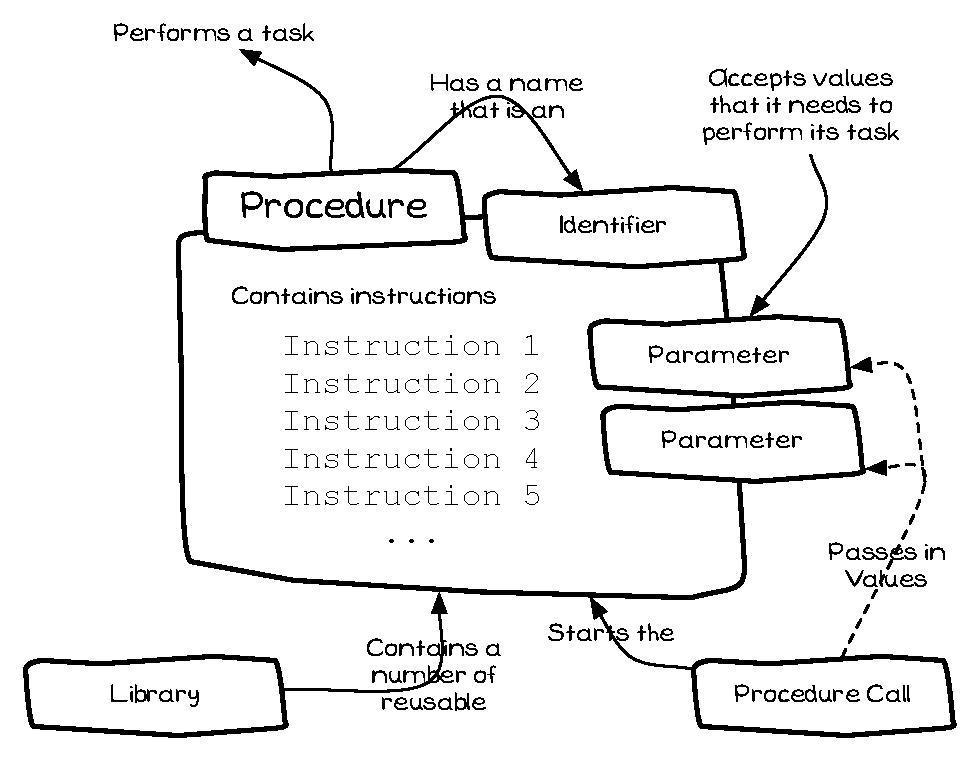
\includegraphics[width=\textwidth]{./topics/program-creation/diagrams/Procedure} 
   \caption[Procedure Concept Diagram]{A Procedure contains instructions to perform a task, and may need to be passed data in order to do this}
   \label{fig:program-creation-procedure}
\end{figure}


\mynote{
\begin{itemize}
  \item Figure \ref{fig:program-creation-procedure} shows the concepts related to Procedures.
  \item A Procedure is a programming artefact that can be called to perform a certain task.
  \item The name of a Procedure is an \nameref{sec:program-creation-identifier}.
  \item Each \nameref{sec:program-creation-library} will contain a number of Procedures to perform common tasks.
  \item The standard library will include procedures to write values to the console.
  \item The SwinGame libraries contain procedures that can draw images on the screen, play sounds, and perform other tasks needed to create small games.
  \item Procedures are also called \textbf{subroutines}, \textbf{sub programs}, \textbf{methods} or \textbf{sub procedures}.
\end{itemize}
}

% section program (end)
\clearpage
\subsection{Expression} % (fold)
\label{sub:expression}

An Expression is a value used in a \nameref{sec:program-creation-statement}. These values may be calculated or entered directly into the source code of the Program.

\begin{figure}[h]
   \centering
   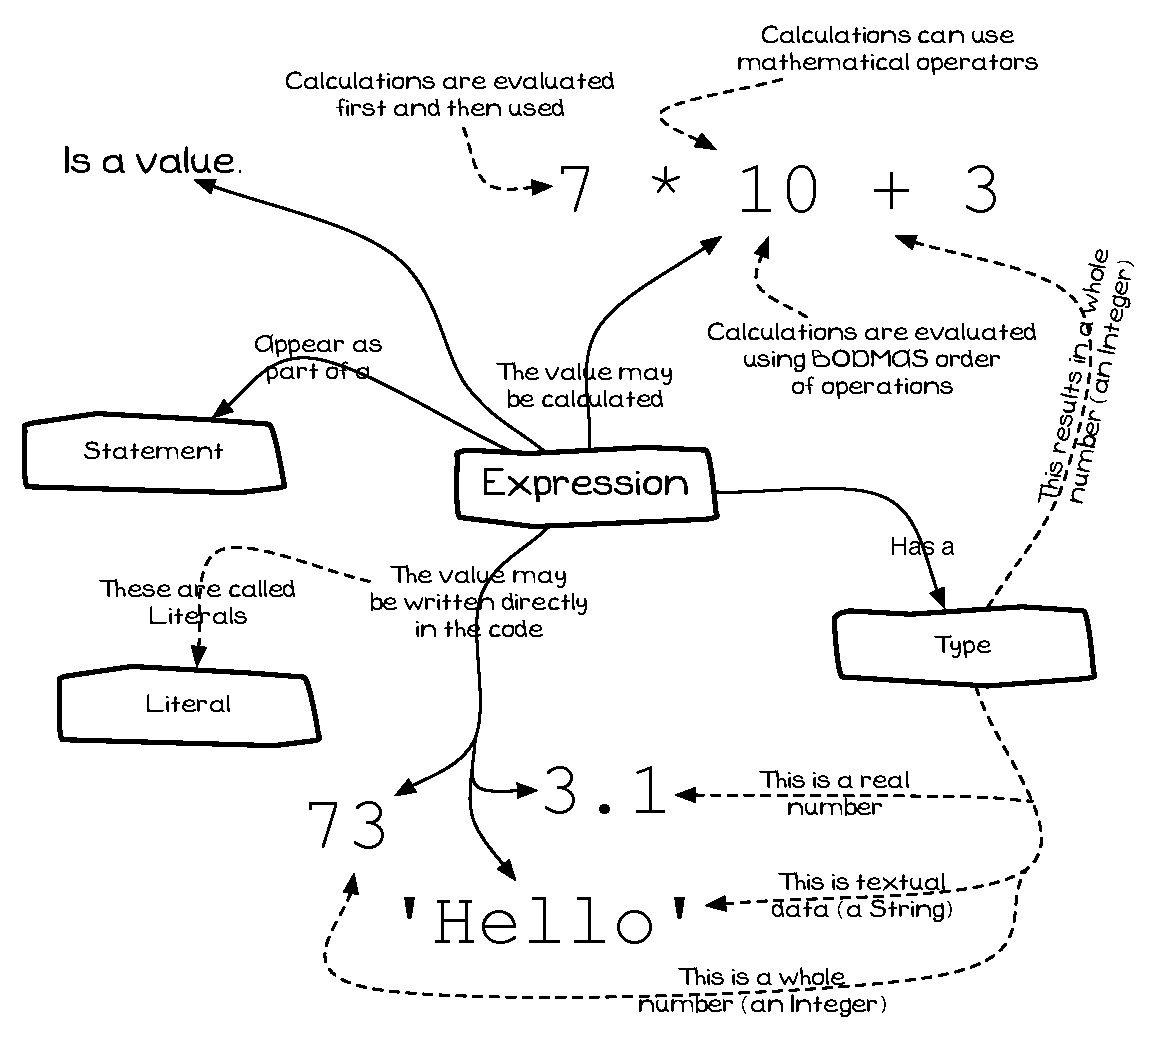
\includegraphics[width=\textwidth]{./topics/program-creation/diagrams/Expression} 
   \caption[Expression Concept Diagram]{An Expression provides a \textbf{value} to be used in a Statement.}
   \label{fig:program-creation-expression}
\end{figure}


\mynote{
\begin{itemize}
  \item The concepts related to Expressions are shown in Figure \ref{fig:program-creation-expression}.
  \item An Expression provides a \textbf{value} that is used in a Statement.
  \item The Expression's value may be calculated or entered directly into the code.
  \item Calculations can use mathematical operators: + for addition, - for subtraction, * for multiplication, $/$ for division, and parenthesis ( ) for grouping.
  \item Expressions are evaluated using the BODMAS order of operations.
  \item Values entered directly within an Expression are \textbf{Literal} values.
\end{itemize}
}

% section program (end)
% \clearpage
\subsection{Literal} % (fold)
\label{sec:program-creation-literal}

A Literal is a whole, or part of, an \nameref{sub:expression} where the value is entered directly into the code.

\begin{figure}[h]
   \centering
   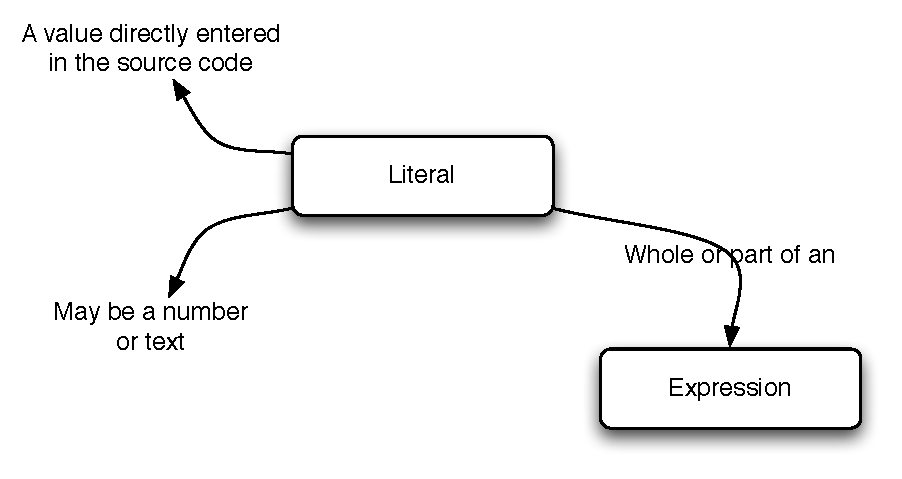
\includegraphics[width=0.8\textwidth]{./topics/program-creation/diagrams/Literal} 
   \caption[Literal Concept Diagram]{Concepts related to Literals.}
   \label{fig:program-creation-literal}
\end{figure}


\mynote{
\begin{itemize}
  \item Figure \ref{fig:program-creation-literal} shows the concepts relate to Literals.
  \item A Literal is a value entered directly into the program's source code.
  \item The value of a Literal can be a number or text.
  \item A Literal can be part or all of an \nameref{sub:expression}.
  \item These values are \emph{hard coded} into the program.
\end{itemize}
}

% section program (end)
\clearpage
\subsection{Type} % (fold)
\label{sub:type}

All values within a program will have a type. The type indicates how the data stored in the computers memory is interpreted by the program. There are three basic data types available in a programming language.

\begin{itemize}
    \item \textbf{Textual} data such as `\emph{Fred}', `\emph{Hello World}', `\emph{23}', and `\emph{This is text!}'.
    \item \textbf{Whole numbers} such as \emph{1}, \emph{0}, \emph{-5}, and \emph{37}.
    \item \textbf{Real numbers} such as \emph{0.5}, \emph{-126.0}, \emph{3.141516}, and \emph{23.981}.
\end{itemize}

\begin{figure}[h]
   \centering
   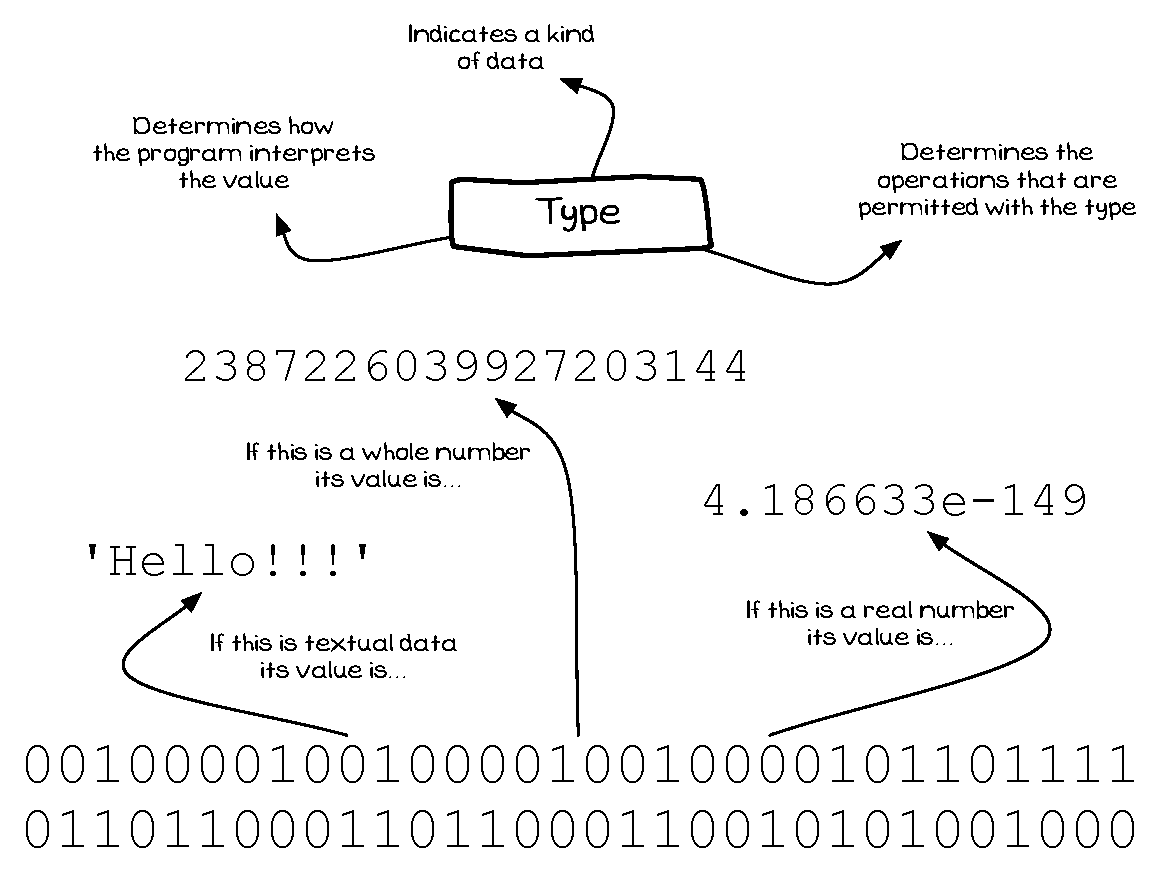
\includegraphics[width=0.95\textwidth]{./topics/program-creation/diagrams/Type} 
   \caption{Types defines how values are interpreted, and the operations that can be performed on the data}
   \label{fig:program-creation-type}
\end{figure}

\mynote{
\begin{itemize}
  \item A type is an \textbf{artefact}, there will be a number of existing types that you can use, and later you will see how to create your own types.
  \item The concepts related to expressions are shown in Figure \ref{fig:program-creation-type}.
  \item A type is a programming artefact that indicates a kind of data.
  \item The type determines the basic actions that can be performed on the value.
  \item The type determines the amount of memory needed to store a value of that kind.
  \item Whole numbers are usually called \textbf{Integers}.
  \item Real numbers are usually represented as \textbf{Floating Point} values. These values have a limited precision, supporting only a certain number of digits of precision.
  \item Textual values can contain numbers. In these cases the number are just textual representations of the values. For example, the text `\emph{23}' is the character `\emph{2}' followed by the character `\emph{3}', it is not the number \emph{23}.
  \item You can perform mathematic operations on numeric data, but not on textual data.
\end{itemize}
}

% section program (end)
\clearpage
\subsection{Identifier} % (fold)
\label{sub:identifier}

An Identifier is the technical term for the words that \emph{identify} something for the compiler. These can be the \textbf{name} of a programming artefact such as a Program, Library, or Procedure, or the words that have special means for the compiler. You will use Identifiers to name the artefact you create, and to select the appropriate artefact when it is used.

\begin{figure}[h]
   \centering
   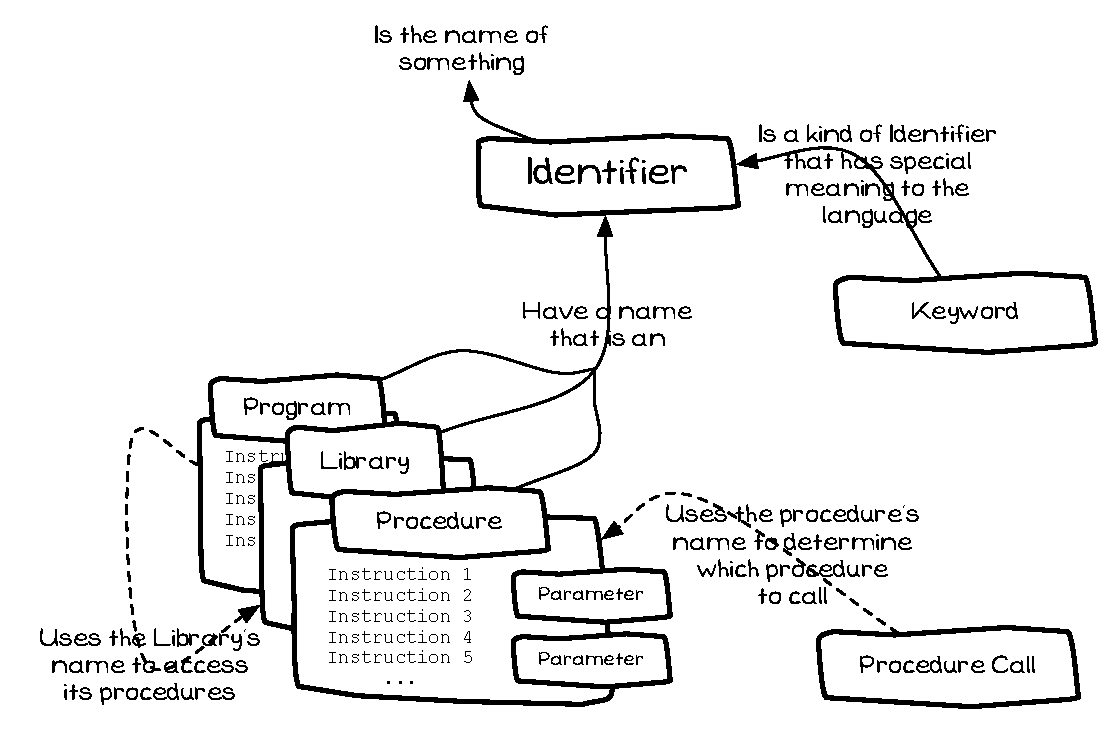
\includegraphics[width=\textwidth]{./topics/program-creation/diagrams/Identifier} 
   \caption[Identifier Concept Diagram]{An Identifier is the name of a programming artefact such as a Program, Library, or Procedure.}
   \label{fig:program-creation-identifier}
\end{figure}


\mynote{
\begin{itemize}
  \item Figure \ref{fig:program-creation-identifier} shows the concepts related to an Identifier.
  \item An Identifier is a \textbf{name} used to identify a programming artefact such as a \nameref{sub:program}, \nameref{sec:program-creation-library} or \nameref{sub:procedure}.
  \item The name you give your Program is an Identifier.
  \item You use Identifiers to indicate which Libraries you want to access in your Program.
  \item The \nameref{sub:procedure call} uses the Procedure's identifier to determine which procedure is called.
\end{itemize}
}

% section program (end)
\clearpage
\subsection{Library} % (fold)
\label{sec:program-creation-library}

A Library is a collection of reusable code artefacts. Each programming language has its own Library, and your programs can make use of the code available in this library.

\begin{figure}[h]
   \centering
   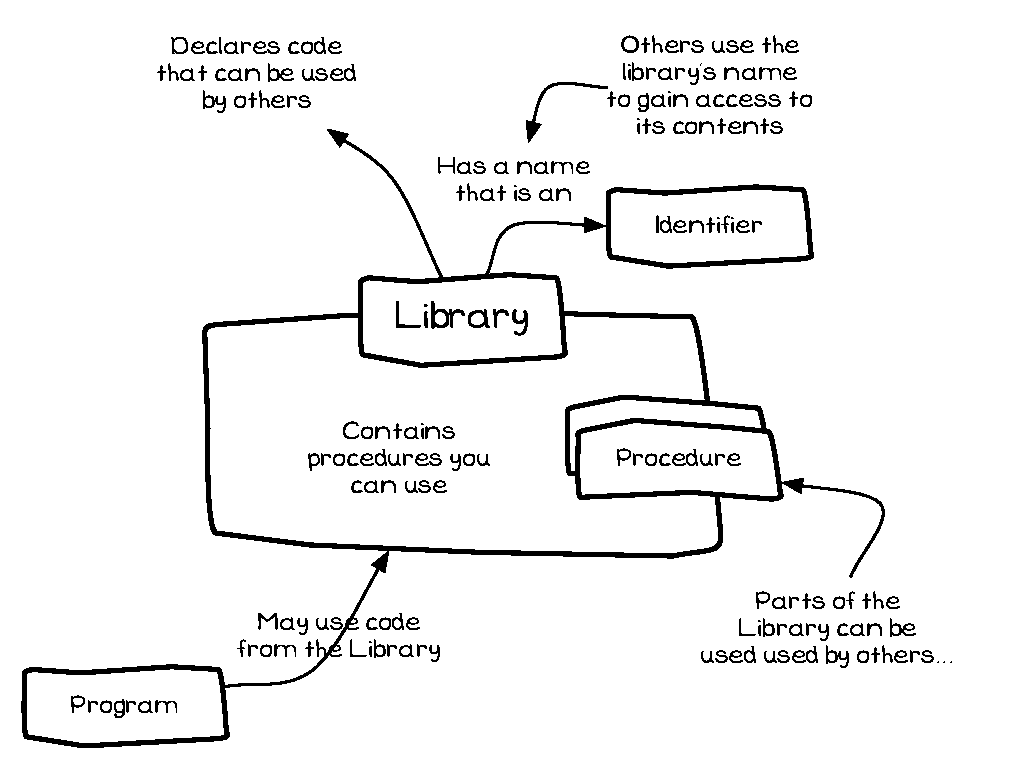
\includegraphics[width=\textwidth]{./topics/program-creation/diagrams/Library} 
   \caption[Library Concept Diagram]{A Library contains code that can be used by your Program}
   \label{fig:program-creation-library}
\end{figure}


\mynote{
\begin{itemize}
  \item Figure \ref{fig:program-creation-library} shows the concepts related to a Library.
  \item A Library is a collection of reusable code artefacts that you can use to perform certain tasks.
  \item The Library will contain \nameref{sub:procedure}s that perform a number of tasks.
  \item Each language has a standard library with code to perform many commonly performed tasks.
  \item Other libraries extend the capability of the languages further.
  \item SwinGame is a Library containing code to help you build games.
\end{itemize}
}

% section program (end)
\clearpage
\subsection{Comments} % (fold)
\label{sub:comments}

A program's source code contains instructions for the actions the computer must perform. However, this code is written and maintained by people. It is often useful to be able to place comments in the code to help someone reading that code understand how the code works or what it is trying to achieve. This text is not something that should be translated into machine code.

Programming languages include the ability to embed \emph{comments} that are ignored by the compiler when it compiles the code.

\bigskip

\mynote{
\begin{itemize}
  \item It is good practice to place a comment at the top of your code explaining what the program does.
  \item Comments should be included to help other people read your code. You will also find these comments useful when you return to your code after a long break.
  \item Make your comments meaningful, try to capture your intentions and ideas.
  \item Comments have no impact on the executable produced by the compiler.
\end{itemize}
}

% subsection comments (end)

% section program_creation_concepts (end)

\clearpage
\subsection{Summary} % (fold)
\label{sub:program_creation_concepts_summary}

This section has introduced a number of programming artefacts, some programming terminology, and one kind of instruction. An overview of these concepts is shown in Figure \ref{fig:program-creation-summary}. The next section will look at how you can use these concepts to design some small programs.

\begin{figure}[h]
   \centering
   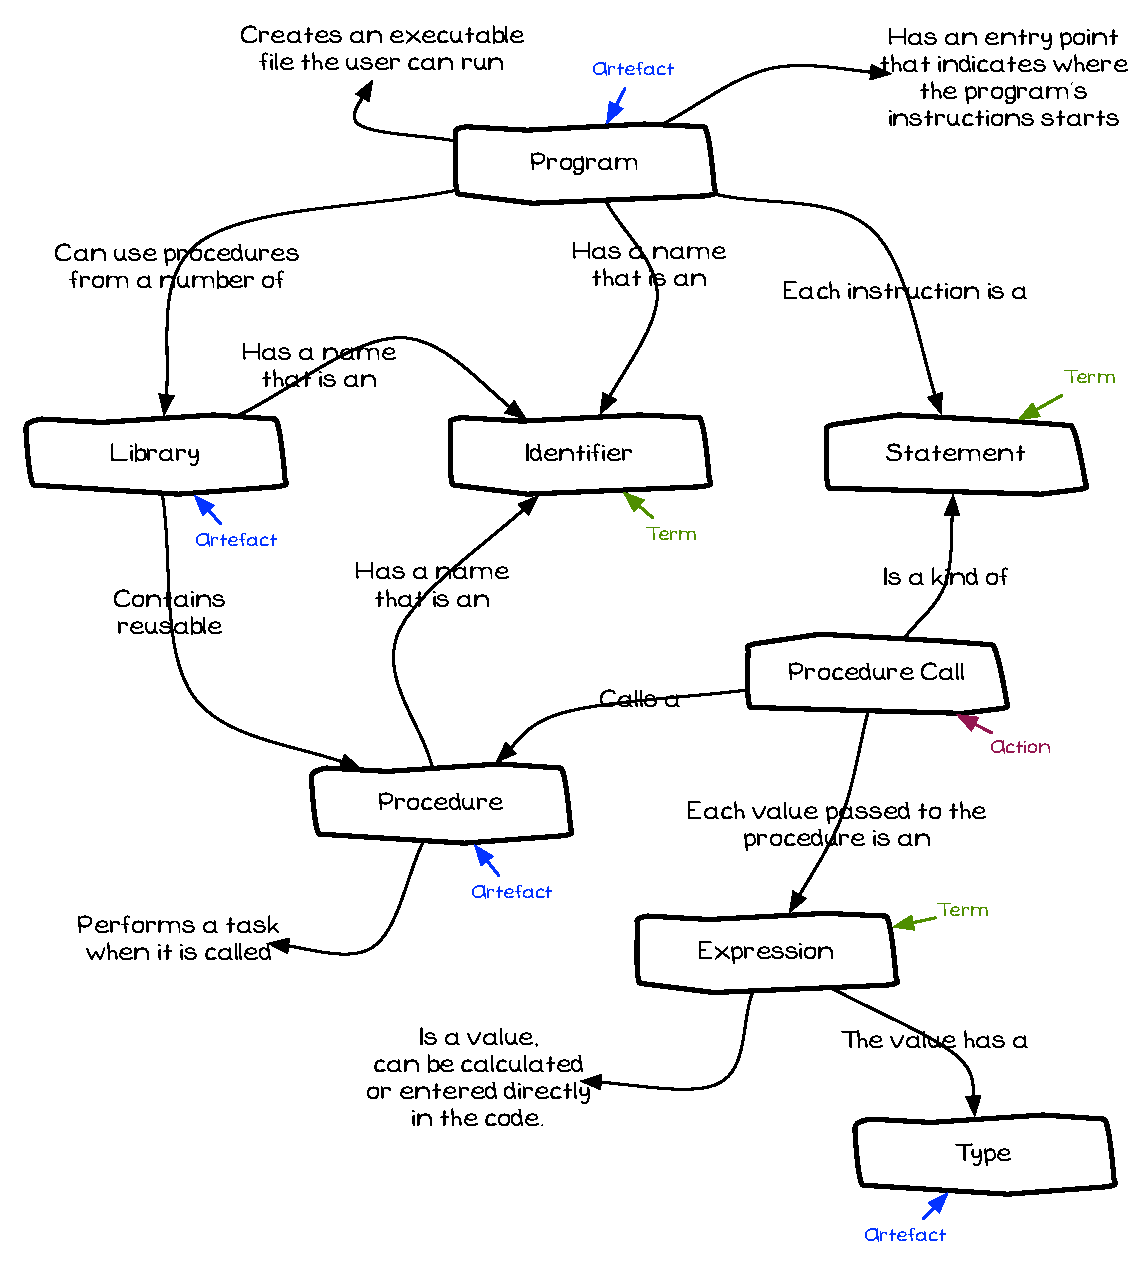
\includegraphics[width=\textwidth]{./topics/program-creation/diagrams/Summary} 
   \caption[Chapter Concepts]{Key Concepts introduced in this Chapter}
   \label{fig:program-creation-summary}
\end{figure}

\mynote{
\begin{itemize}
  \item \textbf{Artefacts} are things you can \emph{create} and \emph{use}.
  \item \textbf{Terms} are things you need to \emph{understand}.
  \item \textbf{Actions} are things you can \emph{command} the computer to perform.
\end{itemize}
}

% subsection summary (end)


% ======================
% = Using the Concepts =
% ======================

\clearpage
\section{Using these Concepts} % (fold)
\label{sec:using_these_concepts_program_creation}

Armed with the knowledge you have gained in the Section \ref{sec:program_creation_concepts} you can now start to design a small program.

\subsection{Designing Output Test} % (fold)
\label{sub:designing_hello_world}

Our first programming task is to extended the classic `Hello World' program to also output some data values, which we will call \textbf{Output Test}. This program will allow you to see all of the different concepts from this chapter in action. A description of the program is shown in Table \ref{tbl:program-creation-hello world description}, and a sample execution is shown in Figure \ref{fig:program-creation-helloworld2}.

\begin{table}[h]
\centering
\begin{tabular}{l|p{12cm}}
  \hline
  \multicolumn{2}{c}{\textbf{Program Description}} \\
  \hline
  \textbf{Name} & \emph{Output Test} \\
  \\
  \textbf{Description} & Displays the text \textbf{`Extended Hello World!'} on the Terminal, followed by \\
                       & \textbf{` 1 + 1 = '} and the result of the calculation 1 + 1, and then \\
                       & \textbf{` Area of a circle with radius 3 = '} and the result of calculating this value. \\
  \hline
\end{tabular}
\caption[Output Test Description]{Description of the \emph{Output Test} program.}
\label{tbl:program-creation-hello world description}
\end{table}

\begin{figure}[h]
   \centering
   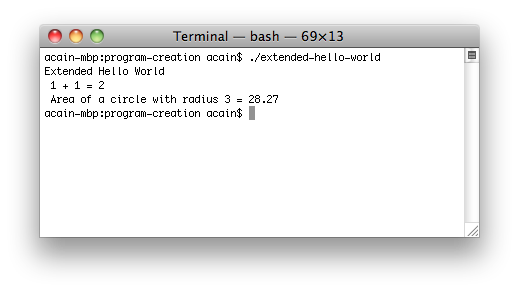
\includegraphics[width=\textwidth]{./topics/program-creation/images/HelloWorld} 
   \caption{Output Test run from the Terminal}
   \label{fig:program-creation-helloworld2}
\end{figure}

To design and implement this program we need to follow a number of steps:

\begin{enumerate}
  \item Understand the problem, and get some ideas on the tasks that need to be performed
  \item Choose the artefacts we will create and use
  \item Map these artefacts to code
  \item Compile and run the program
\end{enumerate}


% \begin{enumerate}
%   \item Determine the programming artefacts that you will need for the program; covered in section \ref{sub:choosing_artefacts_hello_world}. To do this you will need to:
%   \begin{itemize}
%     \item Decide which artefacts to \textbf{create}.
%     \item Select artefacts to \textbf{use} from the Libraries.
%   \end{itemize}
%   \item Determine the sequence of instructions you will need to give the computer for it to use these artefacts to produce the outcome you are looking for.
% \end{enumerate}


% subsection designing_hello_world (end)
\clearpage
\subsection{Understanding Output Test} % (fold)
\label{sub:understanding_output_test}

The first step in creating a program is to analyse the problem, and find related material that we can use to make sure we know what the computer needs to do. You need to understand what the program needs to do before you can start to design the solution.

For this program you need to understand how to calculate the answer of the equation 1 + 1, which is a trivial task, and also how to calculate the area of a circle given its radius. A quick search of the internet and you can find the equation is $PI \times r^2$. Using these equations you have the knowhow needed to calculate the values needed to be output.

% subsection understanding_output_test (end)
\subsection{Choosing Artefacts for Output Test} % (fold)
\label{sub:choosing_artefacts_hello_world}

Designing a program is all about making decisions around how to organise the program's instructions. This means \textbf{deciding} on which artefacts you will \textbf{create}, and which you will \textbf{use}. This chapter has introduced the concept of \textbf{creating} a \nameref{sub:program}, and \textbf{using} \nameref{sub:procedure}s. With these tools it is possible to design simple programs that will get the computer to perform actions by running Procedures in sequence.

The design of \emph{Output Test} requires:

\begin{itemize}
  \item The \textbf{creation} of a \nameref{sub:program}. This Program will contain the instructions to write the three messages to the Terminal.
  \item The \textbf{use} of a procedure to write to the Terminal. Programming languages provide a standard \nameref{sub:library} that, amongst other things, contains procedures to write data to the Terminal. This means you can call one of these procedures, passing it the data you want written to the Terminal, and let it take care of the details of how this is done.
\end{itemize}

\bigskip

The design for this program can be documented using a language neutral \textbf{pseudocode}. This isn't code, just a structured textural description of how the program is intended to work. It gives us a way of reasoning about the program we are creating that is independent of the language used to implement it. As this isn't really code it means we can write it without having to worry about the syntax of a specific programming language.

Listing \ref{lst:program-creation-hello-pseudo} shows the pseudocode for the \emph{Output Test} program. This represents the \textbf{Program} that needs to be created, and shows the three \textbf{procedure calls} that need to be made. 

\pseudocode{lst:program-creation-hello-pseudo}{Pseudocode for the Output Test program.}{./topics/program-creation/application/HelloWorld.txt}

\csection{In C the procedure to write data to the Terminal is called \texttt{printf}, see \nameref{sub:c_console_output}.}
\passection{Pascal has two procedures to write data to the Terminal, \texttt{Write} and \texttt{WriteLn}. }

% subsection choosing_artefacts (end)
\clearpage
\subsection{Writing the Code for Output Test} % (fold)
\label{sub:writing_the_code_for_output_test}

The pseudocode in Listing \ref{lst:program-creation-hello-pseudo} contains the instructions that will get the computer to perform the actions needed by the \emph{Output Test} program. These instructions are not in a form that can be used by the Computer, which can only use machine code. The next step is therefore to convert these ideas into source code that a compiler can then turn into machine code.

The following two sections, Section \ref{sec:program-creation-in-c} \nameref{sec:program-creation-in-c} and Section \ref{sec:program-creation-in-pas} \nameref{sec:program-creation-in-pas}, contain a description of the syntax needed to create programs in the C and Pascal programming languages. Each section outlines how to write the code so that it can be understood by the compiler. These are expressed as a number of related syntax rules. You will find the rules that you need to create a Program, the rules for calling a Procedure, and the related rules.

The rules themselves are expressed as \textbf{Syntax Diagrams}. An example diagram is shown in Figure \ref{synt:basic-rule}. This diagram shows the syntax related to two rules, \emph{first rule}, and \emph{second rule}, and shows the four main parts of all the Syntax Diagrams.

\begin{enumerate}
  \item Text found at the start of a line, not contained in a box, is the name of a rule. There are two rules in Figure \ref{synt:basic-rule}: \emph{first rule}, and \emph{second rule}.
  \item The arrows show the order in which the parts of the rule are applied. They start at the rule, and point in the direction you need to follow. Each box pointed to by the arrow represents either another rule to apply, or text that must be entered into the code at that point.
  \item The rectangular boxes on the line indicate points where other rules need to be applied. For example, the node  \tikz \node [nonterminal] {second rule}; within the \emph{first rule} indicates that you \textbf{must} apply the \emph{second rule} at this point.
  \item The boxes with rounded corners represent text that must be entered into the code. For example, the node \tikz \node [terminal] {write in the code}; within the \emph{first rule} indicates that you \textbf{must} write the text `\emph{write in the code}' at this point in your code.
\end{enumerate}

\examplesyntax{synt:basic-rule}{An example rule}{basic_rules}

In order to use these Syntax Diagrams, you must know what it is that you want to write in the code. The rules in Figure \ref{synt:basic-rule} indicate that you can write either a \emph{first rule} or a \emph{second rule}. If you want to write a \emph{first rule} you find that rule in the diagram, and then follow it's arrows. Reading the \emph{first rule} indicates that the \emph{second rule} must be applied first. 

The \emph{second rule} tells you that you must write the text `\emph{stuff to}'. The vertical bar at the end of the line indicates the end of the \emph{second rule}. This means at this stage the code is:

\begin{verb}
  stuff to 
\end{verb}

Having finished the \emph{second rule}, you can return back to finish the \emph{first rule}. This indicates that you need to write `\emph{write in the code}' in the code. This is the last part of the \emph{first rule}, and so the code needed to write a \emph{first rule} from the Syntax Diagram in Figure \ref{synt:basic-rule} is shown below.

\begin{verb}
  stuff to write in the code
\end{verb}

For a more realistic example have a look at the Syntax Diagram in Figure \ref{synt:example-identifier}\footnote{ 
The \tikz \node [meta-terminal] {...}; is used as shorthand to avoid having to list all of the characters between `A' to `Z'.}. This shows the rules you need to follow to code an \nameref{sub:identifier}\footnote{Most programming languages have the same rules for identifiers.} in either C or Pascal.

\examplesyntax{synt:example-identifier}{The Syntax Rules for an Identifier}{identifier}

There are three rules in Figure \ref{synt:example-identifier}, the \textbf{identifier} rule itself which uses the rules \textbf{letter} and \textbf{digit}. These rules show arrows that give you \emph{options}, and the ability to \emph{repeat} parts of the rules.

\begin{itemize}
  \item A \textbf{letter} is one alphabetic character: i.e. one of `A' to `Z' or `a' to `z'. This is an example of options in the syntax, where you follow \textbf{one} of the available arrows.
  \item A \textbf{digit} is a single number: i.e. a number between `0' and `9'.
  
  \item The \textbf{identifier} has a more complicated rule, with the following parts:
  \begin{enumerate}
    \item The first thing in an \nameref{sub:identifier} must be either a \emph{letter} or an underscore ( \_ ).
    \item Following this is an example of another kind of option. Here you have the ability to end the rule, allowing you to have identifiers that are a single character, or you can follow the downward arrow to include other letters, digits, and underscores.
    \item Following the downward arrow you have a new option where you can choose to have either a \emph{letter}, a \emph{digit}, or an underscore as the second character in your identifier.
    \item Continuing after this option you have another option where you can return back to repeat the previous step, allowing you to have identifiers with more than one or two characters.
  \end{enumerate}
\end{itemize}

\subsubsection{Using the Syntax Diagrams} % (fold)
\label{ssub:using_the_syntax_diagrams}

The Syntax Diagrams help you to map a Concept to the actual code that needs to be written in your source code. To use these diagrams you must first know what it is that you want to create or use, and then you can look up the related syntax. This is where the pseudocode code comes into play. It contains a description of the things that need to be created. 

Listing \ref{lst:program-creation-hello-pseudo3} shows the pseudocode for the Output Test program. This tells you what needs to be created; you need to create a \nameref{sub:program}. This means you need to find the syntax that tells you the rules of how a \emph{Program} is written in C or Pascal. 

\pseudocode{lst:program-creation-hello-pseudo3}{Pseudocode for the \emph{Output Test} program (repeated from Listing \ref{lst:program-creation-hello-pseudo})}{./topics/program-creation/application/HelloWorld.txt}

The pseudocode also indicates that you need to find the rules related to \nameref{sub:procedure call}s. For this Program you need to code three procedure calls within the program's instructions. The language's syntax will tell you how you code these instructions, the Syntax for the program will show you where these instructions are written.

% subsubsection using_the_syntax_diagrams (end)

\subsubsection{How the Syntax is Presented} % (fold)
\label{ssub:how_the_syntax_is_presented}

The C and Pascal Syntax needed to create a program are shown in Section \ref{sec:program-creation-in-c} \nameref{sec:program-creation-in-c} and Section \ref{sec:program-creation-in-pas} \nameref{sec:program-creation-in-pas}. Each part of the Syntax is presented on its own page that shows the Syntax Diagram followed by an example and some notes. The best way to approach this is to do the following:

\begin{enumerate}
  \item Find the page with the Syntax rule you are interested in knowing about.
  \item Have a quick look at the Syntax Diagram and the rules it contains. Read each rule, and get a basic feel for how it is going to come together for your program.
  \item Read the example to see one way of using the Rule. The Syntax Diagram can be used to create any number of variations of the rule, the example gives you at least one way these rules can be coded.
  \item Return to the diagram and make sure you can match each part of the example back to the rule that created it.
  \item Now look up any related rules that are not explained on this rule's page. For example, a \nameref{sub:program} will use the \nameref{sub:statement} rule to code its instructions. The actual rule for a Statement will have its own page. When you read the rules for a Program you will need to also find the page with the rules for a Statement so that you know how to code these within the program.
\end{enumerate}

As you follow this process it is also a good idea to try to use these rules in your own program. Have your code editor open, and see if you can follow the rules or mimic the examples to start building your own program's code. You can also try typing in some of the examples to see how they work.

% subsubsection how_the_syntax_is_presented (end)

% subsection writing_the_code_for_output_test (end)

\subsection{Compiling and Running Output Test} % (fold)
\label{sub:compiling_and_running_output_test}

The previous sections have shown the pseudocode for the \emph{Output Test} program. These steps can be coded using either C or Pascal into a source code file. In order to actually use these instructions you will first need to \textbf{compile} the source code file. This will produce an executable file that you can run.

We are going to start using a \textbf{command line compiler}. You will run this compiler within a text based environment, the \textbf{Terminal}. 

\begin{itemize}
  \item On Ubuntu \textbf{Linux} you can find the Terminal in the \textbf{Accessories} folder within \textbf{Applications}. See Figure \ref{fig:program-creation-ubuntu-terminal}.
  \item On \textbf{MacOS} you can find the Terminal in the \textbf{Utilities} folder within \textbf{Applications}. See Figure \ref{fig:program-creation-macos-terminal}.
  \item On \textbf{Windows} you will need to download and install \emph{MinGW}, making sure to select the \emph{MinSYS} option during the install process. The \emph{MinGW Shell} is then the equivalent of Terminal on the other operating systems. You will find this in \textbf{Program Files}, \textbf{MinGW}. See Figure \ref{fig:program-creation-mingw-shell}.
\end{itemize}

\begin{figure}[p]
   \centering
   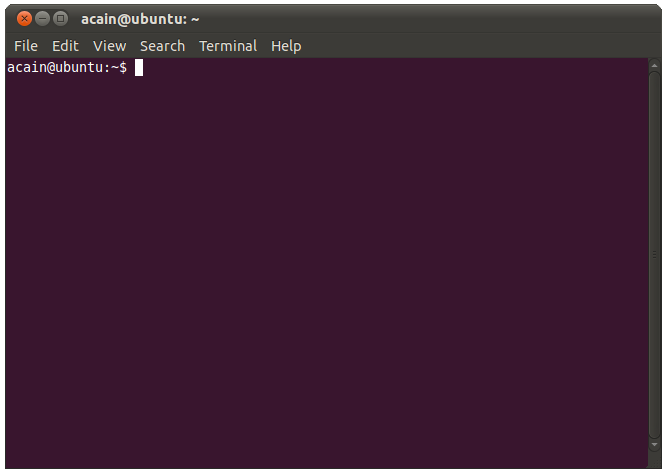
\includegraphics[width=0.6\textwidth]{./topics/program-creation/images/UbuntuTerminal} 
   \caption{Terminal on Ubuntu Linux}
   \label{fig:program-creation-ubuntu-terminal}
\end{figure}

\begin{figure}[p]
   \centering
   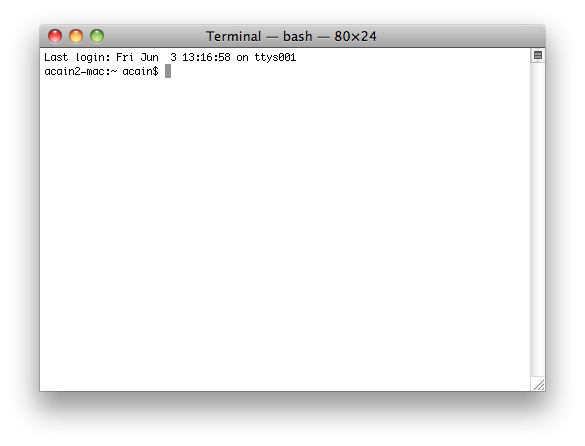
\includegraphics[width=0.6\textwidth]{./topics/program-creation/images/MacOSTerminal} 
   \caption{Terminal on MacOS}
   \label{fig:program-creation-macos-terminal}
\end{figure}

\begin{figure}[p]
   \centering
   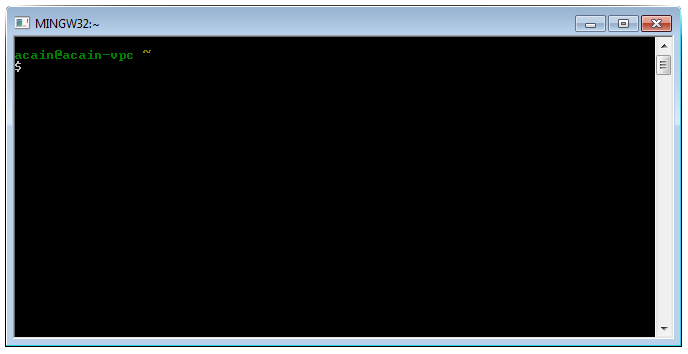
\includegraphics[width=0.6\textwidth]{./topics/program-creation/images/MinGWShell} 
   \caption{MinGW Shell, the Terminal for Windows}
   \label{fig:program-creation-mingw-shell}
\end{figure}

Once you are in the Terminal you have the ability to run a number of text based commands. These commands instruct the computer to perform actions for you.

\begin{itemize}
  \item \textbf{pwd} stands for \emph{Present Working Directory}, and shows you where you are in the file system.
  \item \textbf{ls} stands for \emph{List} and it prints out a list of the files that are in the current directory.
  \item \textbf{cd} stands for \emph{Change Directory} and it moves you to another directory. 
\end{itemize}

To compile your program you need to do the following:

\begin{enumerate}
  \item Change into the directory where your code is located using the \textbf{cd} command. For example, if your code is in a \emph{Code} folder in your \emph{Documents} folder you would use:
  \begin{itemize}
    \item \textbf{Linux}: \texttt{cd /home/username/Documents/Code}
    \item \textbf{MacOS}: \texttt{cd /Users/username/Documents/Code}
    \item \textbf{Windows}: \texttt{cd /c/Users/username/Documents/Code}\footnote{This example moves you into the \texttt{c:{\textbackslash}Users{\textbackslash}username{\textbackslash}Documents{\textbackslash}Code} folder. You need to use the /c/ to refer to the C drive. }
  \end{itemize} 
  \item Run the compiler, passing in the name of the file you want to compile. See the language specific notes below
  \item Execute the program using \texttt{./OutputTest}
\end{enumerate}

\csection{
The C compiler is called \textbf{gcc}. To compile your \emph{Output Test} program you will need to run the following: \bashcode{}{}{code/c/program-creation/compile-output-test.sh}
}

\passection{
The Pascal compiler is called \textbf{fpc}. To compile your \emph{Output Test} program you will need to run the following: \bashcode{}{}{code/pascal/program-creation/compile-output-test.sh}
}

\clearpage
Figure \ref{fig:program-creation-complete-linux-version} shows an example of the instructions needed to compile and run the C version of the \emph{Output Test} program on Linux. Figure \ref{fig:program-creation-complete-linux-version-1} shows an example of the instructions needed to compile and run the Pascal version of the \emph{Output Test} program on Linux.

\begin{figure}[h]
   \centering
   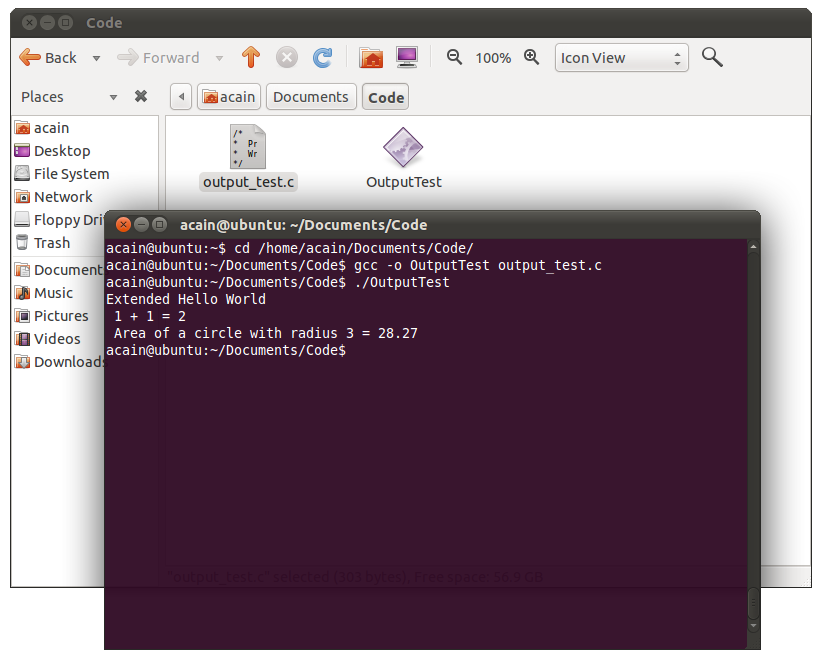
\includegraphics[width=0.62\textwidth]{./topics/program-creation/images/LinuxCompleteExample1} 
   \caption{Example of compiling and running a C version of Output Test on Linux}
   \label{fig:program-creation-complete-linux-version}
\end{figure}

\begin{figure}[h]
   \centering
   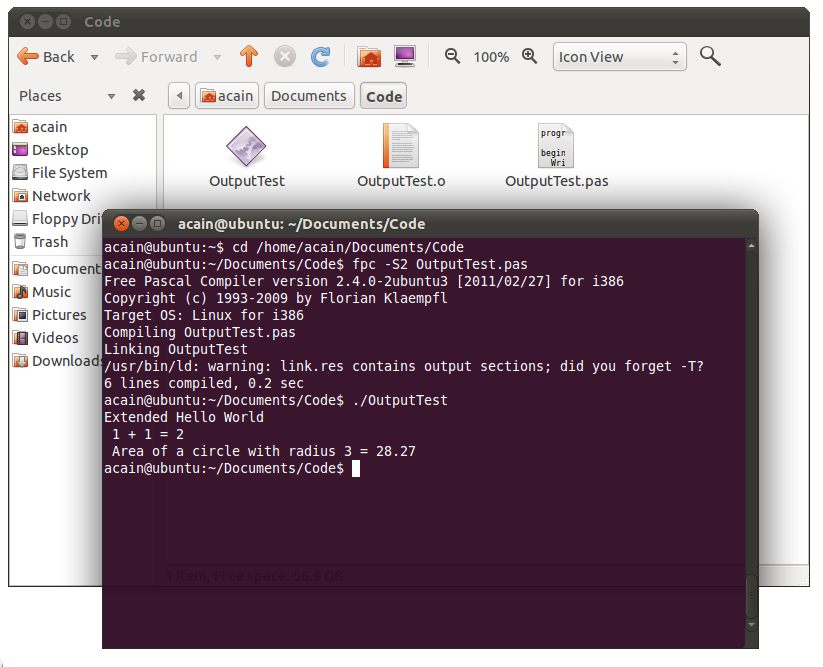
\includegraphics[width=0.62\textwidth]{./topics/program-creation/images/LinuxCompleteExample} 
   \caption{Example of compiling and running a Pascal version of Output Test on Linux}
   \label{fig:program-creation-complete-linux-version-1}
\end{figure}

\clearpage
Figure \ref{fig:program-creation-complete-macos-version} shows an example of the instructions needed to compile and run the C version of the \emph{Output Test} program on MacOS. Figure \ref{fig:program-creation-complete-macos-version-1} shows an example of the instructions needed to compile and run the Pascal version of the \emph{Output Test} program on MacOS.

\begin{figure}[h]
   \centering
   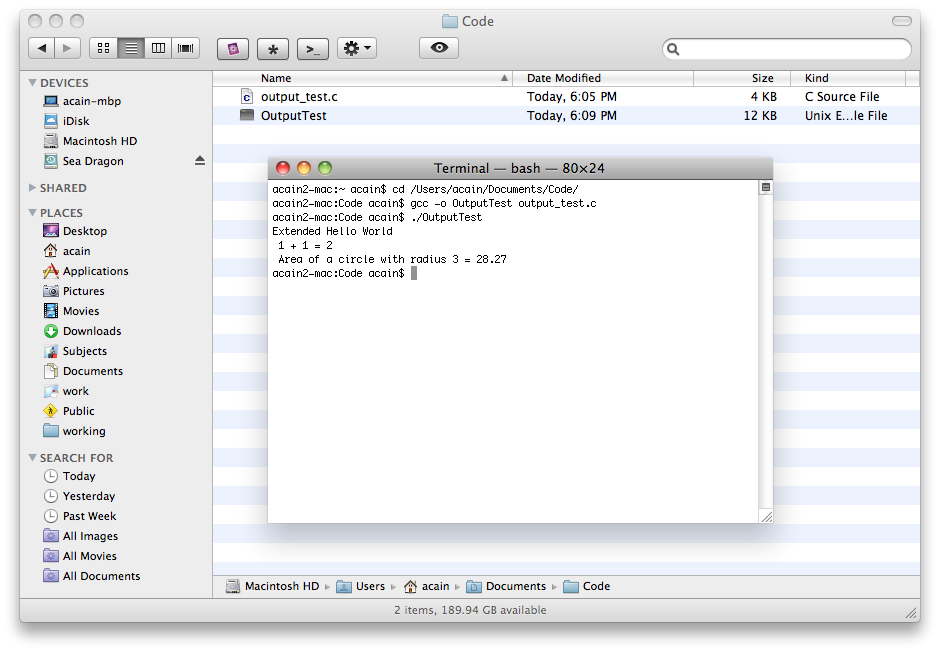
\includegraphics[width=0.73\textwidth]{./topics/program-creation/images/MacOSCompleteExample1} 
   \caption{Example of compiling and running a C version of Output Test on MacOS}
   \label{fig:program-creation-complete-macos-version}
\end{figure}

\begin{figure}[h]
   \centering
   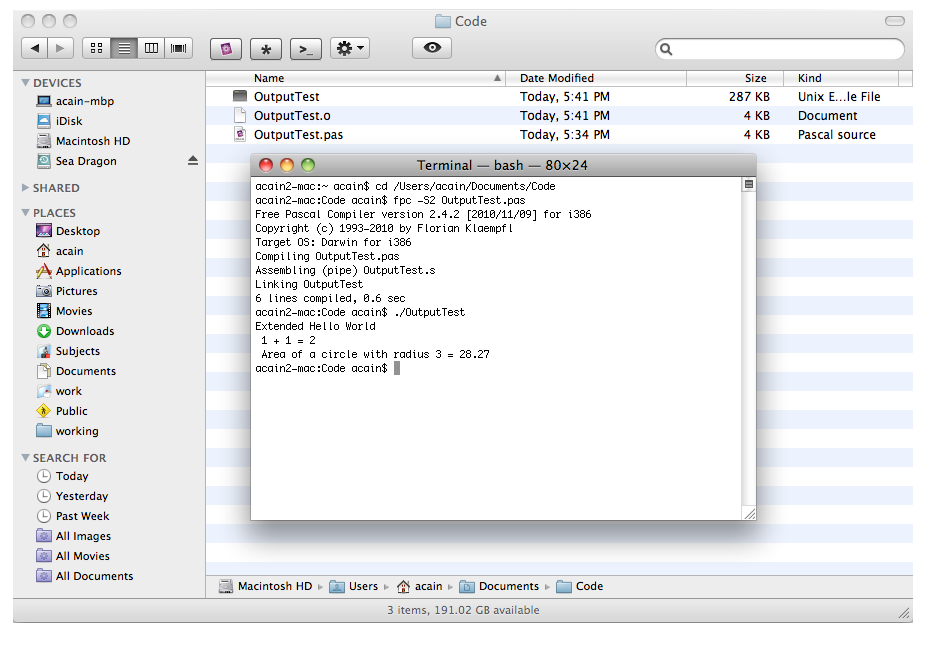
\includegraphics[width=0.73\textwidth]{./topics/program-creation/images/MacOSCompleteExample} 
   \caption{Example of compiling and running a Pascal version of Output Test on MacOS}
   \label{fig:program-creation-complete-macos-version-1}
\end{figure}

\clearpage
Figure \ref{fig:program-creation-complete-windows-version} shows an example of the instructions needed to compile and run the C version of the \emph{Output Test} program on MacOS. Figure \ref{fig:program-creation-complete-windows-version-1} shows an example of the instructions needed to compile and run the Pascal version of the \emph{Output Test} program on MacOS.

\begin{figure}[h]
   \centering
   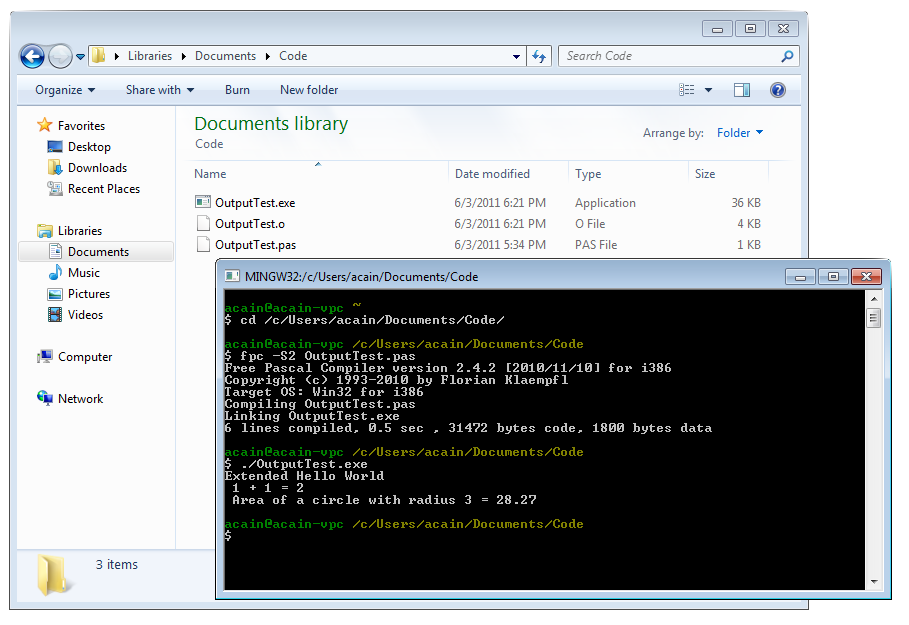
\includegraphics[width=0.73\textwidth]{./topics/program-creation/images/WindowsCompleteExample} 
   \caption{Example of compiling and running a C version of Output Test on Windows}
   \label{fig:program-creation-complete-windows-version}
\end{figure}

\begin{figure}[h]
   \centering
   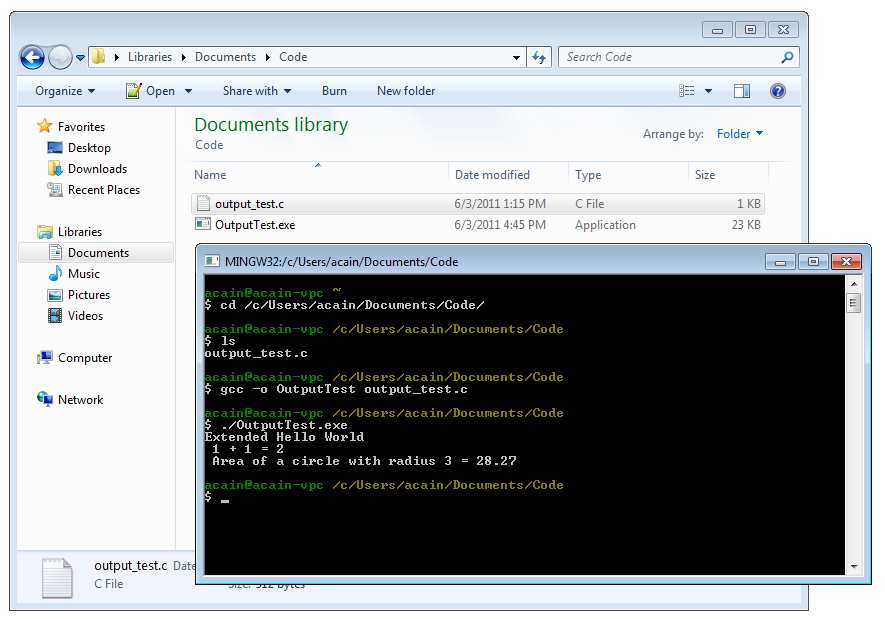
\includegraphics[width=0.73\textwidth]{./topics/program-creation/images/WindowsCompleteExample1} 
   \caption{Example of compiling and running a C version of Output Test on Windows}
   \label{fig:program-creation-complete-windows-version-1}
\end{figure}

% subsection compiling_and_running_output_test (end)
\clearpage
\subsubsection{Compiler Errors} % (fold)
\label{ssub:compiler_errors}

The compiler is a very sensitive piece of software. It requires that you follow the language's syntax precisely. One small mistake, and the compiler will fail to compile your program and end with an error message. This is further complicated by the fact that in many cases the compiler's error messages can appear cryptic.

Here are some handy hints related to dealing with compiler errors.

\begin{enumerate}
  \item \textbf{Know that errors are inevitable}. You will get compiler errors. As you gain more experience you will get fewer errors, but it will always be a rare event that everything is exactly as it should be the first time.
  \item \textbf{Start with the first error message, and do not move on until its fixed}. The compiler will read your code from the top down. So the first error it outputs will be the first in the file. The problem is that the compiler will try to continue on, despite the error. This can mean that other errors further on it the output were actually caused by the compiler being \emph{confused} due to the first error. By fixing the first error you may also fix subsequent errors, as you gain experience you will learn to work out which errors are genuine, and which were caused by previous errors.
  \item \textbf{Deal with one error at a time}. Its easy to feel overwhelmed when you see a huge list of errors, but do not be scared off. Start at the first error, and solve them one by one. Compile after fixing each problem to see if the others are real, or if they were a result of the previous error.
  \item \textbf{Do not add more code until the errors are fixed}. Compile your program frequently. Add small pieces of functionality, and then fix any syntax errors before adding the next piece of functionality. Coding in this way makes sure that you should not get too many errors, and reduces the code you have to search in order to fix the problem.
  \item \textbf{Read the error message carefully}. The message will try to tell you what has gone wrong, and once you understand what the messages are trying to say you will be able find and fix the issues quickly.
  \item  \textbf{Work out what the error messages mean}. Understanding the error messages will mean that you will know what to look for, and will help you avoid these errors in the future. If your not sure what an error message means ask others developers or search for the message on the internet.
  \item \textbf{Find the line and character number of the error}. One important detail in the error message will be the line number of the error. This gives you a starting point to help you locate the problem. Its important to note that this is where the compiler got to when it noticed the error. This \emph{does not} guarantee that this is where the error actually is, but it is a good place to start looking. In some cases this will be the location of the error, in others you may need to look back one or more lines to find the actual source of the problem.
  \item \textbf{Watch for typos}. It is easy to mistype an identifier. When this happens the compiler will not know what to do. Make sure you check for these tiny typos when you get errors related to the compiler not being able to find an identifier.
  \item \textbf{When you get stuck ask for help}. Compiler errors are likely to be something small, but something these small things are hard to find. If you get stuck ask for help. Having access to other more experienced developers will be a valuable resource as you learn to program. Learning to program can be tough at times, and having someone who can help you will make all the difference.
\end{enumerate}


% subsubsection compiler_errors (end)



% section using_these_concepts (end)


% =============
% = C Section =
% =============
\clearpage
\def\pageLang{c}
\section{Program Creation in C}
\label{sec:program-creation-in-c}

% Overview of concepts in C
Section \vref{sec:using_these_concepts_program_creation} of this chapter introduced an `Output Test' program, and its design. The pseudocode from this section is shown in Listing \ref{lst:program-creation-hello-pseudo 1}. In this Section you will see the rules for translating this program's design into the C code shown in Listing \ref{lst:program-c-output_test}.

\pseudocode{lst:program-creation-hello-pseudo 1}{Pseudocode for Hello World program (from Listing \ref{lst:program-creation-hello-pseudo}).}{./topics/program-creation/application/HelloWorld.txt}

\csection{\ccode{lst:program-c-output_test}{Output Test in C}{code/c/program-creation/output_test.c}}

\mynote {
\begin{itemize}
  \item Save the C code in a file named \texttt{output\_test.c}.
  \item Compile this using \bashsnipet{gcc -o:OutputTest output_test.c}.
  \item Run using \bashsnipet{./OutputTest}.
  \item The code at the start is a Comment describing what is in the file, see \nameref{sub:c_comments}.
  \item The code \csnipet{#include <stdio.h>}, is part of the \nameref{sub:program_in_c}. It is a \emph{header include}, and gives access to the code in the \emph{Standard IO} Library.
  \item \csnipet{int main() { ... }} is part of the \nameref{sub:program_in_c}, it marks the entry point and contains the instructions that are executed when the program runs.
  \item The \texttt{main} function contains three \nameref{sub:program-creation-c_procedure_call}s. Each is a call to the \texttt{printf}. \nameref{sub:procedure}, which is used to output text to the console. See \nameref{sub:c_console_output}.
  \item Each of the procedure calls contains one or two \nameref{sub:expression}s that pass values to the \texttt{printf} procedure, which will output these to the Terminal.
  \item This code uses \texttt{c-strings}, \texttt{int}, and \texttt{float} types, see \nameref{sub:program-creation-c_types}.
\end{itemize}
}

% Each part of the syntax
% \clearpage
% \subsection{C++ Program} % (fold)
% \label{sub:program_in_c}

% The C++ programming language does not have an explicit Program artefact for you to create. Rather, in C++ a program is implied by the existence of a special function called `\texttt{main}' somewhere in your source code. Figure \ref{csynt:program-creation-program} shows the structure of the syntax you can use to create a program using the C++ language.

% \csyntax{csynt:program-creation-program}{a Program}{program-creation/program}

% The code in Listing \ref{lst:program-creation-c-hello-world} shows an example C++ Program. You should be able to match this up with the syntax defined in Figure \ref{csynt:program-creation-program}. Notice at the start of the code the syntax indicates we can have an optional \emph{header include}, this matches up with the first line in the code where it \emph{includes} the `splashkit.h' header file. Declaration of the \texttt{main} function follows the inclusion of the header file, and it contains the instructions that are executed when the program runs.

% \csection{\ccode{lst:program-creation-c-hello-world}{C++ Hello World}{code/c/program-creation/hello-world.c}}

% \mynote{
%   \begin{itemize}
%     \item When a C++ \nameref{sub:program} runs, it start running the instructions from the first \nameref{sub:statement} within the \texttt{main} function (line 5).
%     \item A \nameref{sub:function} is a kind of \nameref{sub:procedure}, and their details will be covered later (see \sref{sub:function}).
%     \item The `\texttt{return 0}' code is a \nameref{sub:statement} that ends the \texttt{main} function (and the program). The \nameref{sub:return_statement} is covered later in \sref{sub:return_statement}.
%     \item With the \emph{header include} syntax you use \csnipet{#include <...>} to include standard libraries, and \csnipet{#include "..."} to include other external libraries.
%     \item Header files contain a summary of the features available within a library. By including the header file you gain access to these features.
%   \end{itemize}
% }

% % subsection program_in_c (end)
\clearpage
\subsection{C Statement} % (fold)
\label{sub:program-creation-c_statement}

In a \nameref{sec:program-creation-statement} you are commanding the computer to perform an action. There are only a small number of statements you can choose from. At this stage the only statement is the \nameref{sub:procedure call}, known as the \emph{procedure statement} in C. This is shown in Figure \ref{csynt:program-creation-statement}, where we can see that at this stage all Statements are calls to \nameref{sub:procedure}s.

\csyntax{csynt:program-creation-statement}{Statement Syntax}{program-creation/statement}

\csection{\ccode{lst:program-creation-c-knights}{C Knights}{code/c/program-creation/knights.c}}

\mynote{
\begin{itemize}
  \item The code in Listing \ref{lst:program-creation-c-knights} contains a \nameref{sub:program_in_c}.
  \item This Program contains five procedure calls, see \nameref{sub:program-creation-c_procedure_call}.
  \item Each procedure call runs the \texttt{printf} procedure to output text to the console. See the section on \nameref{sub:c_console_output}.
\end{itemize}
}


% subsection c_statement (end)
\clearpage
\subsection{C Procedure Call} % (fold)
\label{sub:program-creation-c_procedure_call}

A Procedure Call allows you to run the code in a Procedure, getting its instructions to run before control returns back to this point in the Program.

\csyntax{csynt:program-creation-procedure-call}{Procedure Call Syntax}{program-creation/procedure-call}

\csection{\ccode{lst:program-creation-c-count-back}{C Count Back}{code/c/program-creation/count-back.c}}

\mynote{
\begin{itemize}
  \item A Procedure Call is an \textbf{action}, it commands the computer to run the code in a Procedure.
  \item The Procedure Call starts with the Procedure's \nameref{sec:program-creation-identifier}, this indicates the procedure to be called.
  \item Following the Identifier is a list of values within parenthesis,  these are the values (coded as \nameref{sub:expression}s) that are passed to the procedure for it to use.
  \item Remember that C is case sensitive so using \texttt{Printf} instead of \texttt{printf} will not work.
  \item The code in Listing \ref{lst:program-creation-c-count-back} contains a \nameref{sub:program_in_c}.
  \item This Program contains four procedure calls.
  \item Each procedure call runs the \texttt{printf} procedure to output text to the console. See the section on \nameref{sub:c_console_output}.
  
\end{itemize}
}


% subsection c_procedure_call (end)
\clearpage
\subsection{C Identifier} % (fold)
\label{sub:c_identifier}

The C \nameref{sec:program-creation-identifier} syntax is shown in Figure \ref{csynt:program-creation-identifier}. In C, as in most languages, the identifier must start with an underscore (\_) or a letter, in other words your identifiers cannot start with a number or contain other symbols. This is because the compiler needs a way of distinguishing identifiers from numbers entered in the code as Literals.

\csyntax{csynt:program-creation-identifier}{an Identifier}{program-creation/identifier}

\begin{table}[h]
  \centering
  \begin{tabular}{|ccccc||cc|}
    \hline
    \multicolumn{5}{|c||}{\textbf{Keywords}} & \multicolumn{2}{c|}{\textbf{Example Identifiers}} \\
    \hline
    \texttt{auto}     &   \texttt{break}    & \texttt{case}     &   \texttt{char}     &   \texttt{const}   & printf & scanf  \\         
    \texttt{continue} &   \texttt{default}  &  \texttt{do}      &   \texttt{double}   &   \texttt{else}    & bitmap & sound\_effect  \\
    \texttt{enum}     &   \texttt{extern}   & \texttt{float}    &   \texttt{for}      &   \texttt{goto}    & name & draw\_bitmap  \\
    \texttt{if}       &   \texttt{int}      &   \texttt{long}   &   \texttt{register} &   \texttt{return}  & age & my\_alien \\         
    \texttt{short}    &   \texttt{signed}   & \texttt{sizeof}   &   \texttt{static}   &   \texttt{struct}  & height & test  \\          
    \texttt{switch}   & \texttt{typedef}  &   \texttt{union}    &   \texttt{unsigned} &   \texttt{void}    & alien & name3 \\
    \texttt{volatile} &   \texttt{while}    &  & &                                                         & \_23  & i \\
    \hline
  \end{tabular}
  \caption{C Keywords and example Identifiers}
  \label{tbl:program-creation-c identifiers and keywords}
\end{table}












\mynote{
\begin{itemize}
  \item Table \ref{tbl:program-creation-c identifiers and keywords} contains a list of the keywords in C, and some example identifiers.
  \item Each item in Table \ref{tbl:program-creation-c identifiers and keywords} is a valid identifier.
  \item A letter is any alphabetic character (\emph{a} to \emph{z} and \emph{A} to \emph{Z}).
  \item A digit is a single number (\emph{0} to \emph{9}).
  \item A \textbf{keyword} is a kind of identifier that has special meaning to the language. Usually used to identify a kind of action, or a kind of artefact.
  \item Notice in the syntax definition that Identifiers cannot contain spaces, or special characters other than underscores (\_).
\end{itemize}
}

% subsection c_identifier (end)
\clearpage
\subsection{C Expression} % (fold)
\label{sub:program-creation-c_expression}

An \nameref{sub:expression} in C is a mathematical calculation or a Literal value. Each expression will have a \nameref{sub:type}, and can contain a number of mathematic operators. Table \ref{tbl:program-creation-c operators and expresions} lists the operators that you can include in your expressions, listed in order of precedence\footnote{The expressions follow the standard mathematic order of precedence (BODMAS).}. The operators you can use depend on the kind of data that you are using within the expression.

\begin{table}[h]
  \centering
  \begin{tabular}{|c|l|l|}
    \hline
    \textbf{Operator} & \textbf{Description} & \textbf{Example} \\
    \hline
    \texttt{ () }     &   Parenthesis                 & \texttt{(1 + 1) * 2}  \\
    \texttt{* /}      &   Multiplication and Division & \texttt{1 / 2 * 5}    \\
    \texttt{+ -}      &   Addition and subtraction    & \texttt{10 + 3 - 4}   \\
    \hline
  \end{tabular}
  \caption{C Operators and Example Expressions}
  \label{tbl:program-creation-c operators and expresions}
\end{table}

\begin{table}[h]
  \begin{minipage}{\textwidth}
  \centering
  \begin{tabular}{|c|c|l|}
    \hline
    \textbf{Example Expression} & \textbf{Value} & \textbf{Type} \\
    \hline
    \texttt{ 73 }     &   73                 & \texttt{int}  \\
    \texttt{ 2.1 }      & 2.1   & \texttt{float}    \\
    \texttt{ "Hello World" }      &   "Hello World"    & \texttt{char*}   \\
    \texttt{ "Fred" }      &   "Fred"    & \texttt{char*}   \\
    \texttt{ 3 * 2 } & 6 & \texttt{int} \\
    \texttt{ 1 + 3 * 2 }  & 7 & \texttt{int} \\
    \texttt{ (1 + 3) * 2} & 8 & \texttt{int} \\
    \texttt{ 7 - 3 + 1 }  & 5 & \texttt{int} \\
    \texttt{ 3 / 2 } & 1\footnote{C does integer division for int values, rounding the value off.} & \texttt{int} \\
    \texttt{ 3.0 / 2.0} & 1.5 & \texttt{float} \\
    \texttt{ 3 / 2.0 } & 1.5\footnote{If either or both value are real numbers the result is also a real number.} & \texttt{float} \\
    \texttt{ 1 + (3 / 2.0) + 6 * 2 - 8} & 6.5 & \texttt{float} \\
    \hline
  \end{tabular}
\end{minipage}
  \caption{C Operators and Example Expressions}
  \label{tbl:program-creation-c example expresions}
\end{table}


\mynote{
\begin{itemize}
  \item Table \ref{tbl:program-creation-c example expresions} shows some example expressions, their values, and types
  \item Expressions can be Literal values, entered in the code.
  \item Expression can contain mathematical calculations using standard addition, subtraction, multiplication, division, and grouping.
\end{itemize}
}


% subsection c_expression (end)
\clearpage
\subsection{C Literal} % (fold)
\label{sub:program-creation-c_literal}

A Literal is either a number or text value entered directly into the code. Figure \ref{csynt:program-creation-literal} shows the syntax for the different Literal values you can enter into your C code.

\csyntax{csynt:program-creation-literal}{Literals}{program-creation/literal}

\mynote{
\begin{itemize}
  \item Within a string the {\textbackslash} is used to indicate the next character has a special meaning. The following list includes the most useful escape characters:
  \begin{itemize}
    \item \texttt{{\textbackslash}n} creates a new line
    \item \texttt{{\textbackslash}"} creates a double quote
    \item \texttt{{\textbackslash}\%} creates a \% character
    \item \texttt{{\textbackslash}{\textbackslash}} creates a {\textbackslash}
  \end{itemize}
  % \item `0..9' means the digits 0, 1, 2, etc. up to 9.
  \item `\emph{any character except ", {\textbackslash}, \%, or new line}' allows you to include any character, with those that can not be includes directly being able to be included using the escape sequence (e.g. {\textbackslash}n for new line).
\end{itemize}
}

% subsection c_literal (end)
\clearpage
\subsection{C Types} % (fold)
\label{sub:program-creation-c_types}

\nameref{sub:type}s are used to define how data is interpreted and the operations that can be performed on the data. Table \ref{tbl:program-creation-c-types} shows the three basic types of data, the associated C type, size in memory, and other related information. Table \ref{tbl:program-creation-c operators by type} shows the operators that are permitted for each Type.

\begin{table}[h] 
\begin{minipage}{\textwidth}
\centering
\begin{tabular}{|l|c|c|c|}
\hline
\multicolumn{4}{|c|}{\textbf{Whole Number Types}} \\
\hline
\emph{Name} & \emph{Size} & \multicolumn{2}{|c|}{\emph{Range (lowest .. highest)}} \\
\hline
\texttt{short} & 2 bytes/16 bits & \multicolumn{2}{|c|}{-32,767 .. 32,767} \\
\texttt{int} & 4 bytes/32 bits & \multicolumn{2}{|c|}{-2147483648 .. 2147483647} \\
\texttt{long long}    & 8 bytes/64 bits & \multicolumn{2}{|c|}{-9,223,372,036,854,775,807 ..} \\
  & & \multicolumn{2}{|c|}{9,223,372,036,854,775,807} \\
\hline
\multicolumn{4}{c}{} \\
\hline
\multicolumn{4}{|c|}{\textbf{Real Number Types}} \\
\hline
\emph{Name} & \emph{Size} & \emph{Range (lowest .. highest)} & \emph{Significant Digits} \\
\hline
\texttt{float} & 4 bytes/32 bits & 1.0e-38 .. 1.0e38 & 6 \\
\texttt{double} & 8 bytes/64 bits & 2.0e-308 .. 2.0e308 & 10 \\
\hline
\multicolumn{4}{c}{} \\
\hline
\multicolumn{4}{|c|}{\textbf{Text Types}} \\
\hline
\emph{Name} & \emph{Size} & \multicolumn{2}{|c|}{\emph{Known As}} \\
\hline
\texttt{char}  & 1 byte/8 bits & \multicolumn{2}{|c|}{} \\
\hline
\texttt{char*} & various\footnote{1 byte per character + 1 byte overhead} &  \multicolumn{2}{|c|}{c-string} \\
\hline
\end{tabular}
\caption{C Data Types}\label{tbl:program-creation-c-types}
\end{minipage}
\end{table}

\begin{table}[h]
  \centering
  \begin{tabular}{|c|c|l|}
    \hline
    \textbf{Type} & \textbf{Operations Permitted} & \textbf{Notes}\\
    \hline
    Whole Numbers     &   \texttt{( ) + - / *} & Division rounds down if all\\
                                    &                        & values are whole numbers.\\
    Real Numbers   &   \texttt{( ) + - / *} &    \\
       & & \\
    Text           &   \texttt{( ) }          & You cannot perform mathematical\\
    & & operations on text.\\
    \hline
  \end{tabular}
  \caption{C Permitted Operators by Type}
  \label{tbl:program-creation-c operators by type}
\end{table}

\csyntax{csynt:program-creation-typed-literal}{Typed Literals}{program-creation/typed-literal}

\mynote{
\begin{itemize}
  \item The \texttt{int} type is the typical whole number type.
  \item The \texttt{double} type is the typical real number type.
  \item C has limited support for text data. In most languages, text is represented using a \texttt{String} type. The C text type is named \texttt{c-string} to indicate this limited support. C includes a \nameref{sub:library} to add operations to manipulate \texttt{c-string} values.
  \item For example values see Table \vref{tbl:program-creation-c example expresions}.
\end{itemize}
}
% subsection c_types (end)
\clearpage
\subsection{C Terminal Output} % (fold)
\label{sub:c_console_output}

C comes with a range of \nameref{sub:library}s that provide reusable programming artefacts, including reusable \nameref{sub:procedure}s. The Standard Library includes a number of different components, one of which is \texttt{stdio.h}. The \texttt{stdio.h} refers to the Standard Input/Output library. This header file gives you access to artefacts you can use to perform input and output, including code to write output to the Terminal. The \texttt{printf} procedure is used to write data to the Terminal.

\begin{table}[h]
  \centering
  \begin{tabular}{|c|p{9cm}|}
    \hline
    \multicolumn{2}{|c|}{\textbf{Procedure Prototype}} \\
    \hline
    \multicolumn{2}{|c|}{} \\
    \multicolumn{2}{|c|}{\texttt{printf(char *format, \ldots )}} \\
    \multicolumn{2}{|c|}{} \\
    \hline
    \textbf{Parameter} & \textbf{Description} \\
    \hline
    \texttt{ format } & The text that is to be written to the Terminal. This text may contain format tags to include other values. See Figure \ref{csynt:program-creation-format-string} for the syntax of the format tag. \\
    & \\
    \texttt{\ldots}   & Optional values, must have at least as many values as format tags. \\
    \hline
  \end{tabular}
  \caption{Parameters that must be passed to \texttt{printf}}
  \label{tbl:program-creation-c printf parameters}
\end{table}

The syntax for the \texttt{Format Tag} is shown in Figure \ref{csynt:program-creation-format-string}, with the details for the values that can be placed in the \emph{flag}, \emph{width}, \emph{precision}, and \emph{specifier} section being shown in Table \vref{tbl:program-creation-c printf specifier}. A number of examples are shown in Table \ref{tbl:program-creation-c printf specifier}, as well as in Listing \ref{lst:program-creation-c-printf}.

\csyntax{csynt:program-creation-format-string}{Format Tag}{program-creation/format-string}

\csection{\ccode{lst:program-creation-c-printf}{C \texttt{printf} Examples}{code/c/program-creation/sample-printf.c}}

\begin{table}[htbp]
  \begin{minipage}{\textwidth}
  \centering
  
  \begin{tabular}{|c|p{4cm}|l|c|}
    \hline
    \textbf{Flag} & \textbf{Description}  & \multicolumn{2}{c|}{ \textbf{Example Usage \& Output} } \\
    \hline
    \texttt{-}  & Left justify\footnote{Right justify is the default} the width. & \csnipet{printf("\%-5c", 'a');} & \texttt{a\textvisiblespace\textvisiblespace\textvisiblespace\textvisiblespace} \\
                & & \csnipet{printf("\%5i", 23);} & \texttt{\textvisiblespace\textvisiblespace{\textvisiblespace}23} \\
    \hline
    \texttt{+}  & Always display sign for numbers & \csnipet{printf("\%+d", 42);} & \texttt{+42} \\
                & & \csnipet{printf("\%+i", -42);} & \texttt{-42} \\
    \hline
    \texttt{\textvisiblespace}\footnote{A space.}  & Shows a space if positive & \csnipet{printf("\% f", 127.5);} & \texttt{\textvisiblespace127.5} \\
                & & \csnipet{printf("\% i", -73);} & \texttt{-73} \\
    \hline
    \texttt{0}  & Pad with 0's rather than spaces\footnote{The 5 in the example represents the width of the output.} & \csnipet{printf("\%05i", 3);} & \texttt{00003} \\
    \hline
    \multicolumn{4}{c}{} \\
    \hline
    \textbf{Width} & \textbf{Description}  & \multicolumn{2}{c|}{ \textbf{Example Usage \& Output} } \\
    \hline
    \emph{number} & The minimum width for output & \csnipet{printf("\%5i", 1);} & \texttt{\textvisiblespace\textvisiblespace\textvisiblespace{\textvisiblespace}1} \\
    & & \csnipet{printf("\%5s", "Fred");} & \texttt{{\textvisiblespace}Fred} \\
    & & \csnipet{printf("\%5s", "Hello World");} & \texttt{Hello World}\footnote{Width specifies the minimum width.} \\
    \hline
    \multicolumn{4}{c}{} \\
    \hline
    \textbf{Precision} & \textbf{Description}  & \multicolumn{2}{c|}{ \textbf{Example Usage \& Output} } \\
    \hline
    \emph{number} & \textbf{For integers}: same as Width &  \csnipet{printf("\%.5i", 1);} & \texttt{\textvisiblespace\textvisiblespace\textvisiblespace{\textvisiblespace}1} \\
     & \textbf{For real numbers}: number of &  \csnipet{printf("\%.3f", 3.1415);} & \texttt{3.142} \\
     &  values after the decimal point & \csnipet{printf("\%.3f", 2.5);} & \texttt{2.500} \\
    \hline
    \multicolumn{4}{c}{} \\
    \hline
    \textbf{Specifier} & \textbf{Output}  & \multicolumn{2}{c|}{ \textbf{Example Usage \& Output} } \\
    \hline
    \texttt{c}  & A single character & \csnipet{printf("\%c", 'a');} & \texttt{a} \\
    \hline
    \texttt{d} or \texttt{i} & A signed decimal integer & \csnipet{printf("\%d", -127);} & \texttt{-127} \\
    \hline
    \texttt{f}  & Decimal floating point number & \csnipet{printf("\%f", 127.5);} & \texttt{127.5} \\
    \hline
    \texttt{s}  & Text data & \csnipet{printf("\%s", "Hello World");} & \texttt{Hello World} \\
    \hline
    \multicolumn{4}{c}{} \\
    \hline
  \end{tabular}
  
  \end{minipage}
  \caption{Details for Format Tag specifier, flag, precision, and width}
  \label{tbl:program-creation-c printf specifier}
\end{table}





% subsection c_console_output (end)
\clearpage
\subsection{C Comments} % (fold)
\label{sub:c_comments}

Comments allow you to embed documentation and explanatory text within your program's code. The comments are skipped by the compiler, so they have no affect on the program's machine code. You write comments to help other people understand what you intend the program to do.

\csyntax{csynt:program-creation-comment}{comments}{program-creation/comment}

\mynote {
\begin{itemize}
  \item Figure \ref{csynt:program-creation-comment} shows the syntax for comments in C.
  \item In standard C the first style of comments must be used, \csnipet{/* Comment */}.
  \item Most modern C compilers also allow single line comments using \csnipet{// Comment}.
  \item Standard C comments can span multiple lines, these are also known as `\emph{block comments}'.
  \item A compiler ignores comments when compiling your code.
  \item You can type almost anything in the comment, represented by the \texttt{...} in the diagram.
\end{itemize}
}

% subsection c_comments (end)
\clearpage
\subsection{Some Common C Errors with Program Creation} % (fold)
\label{sub:some_common_c_errors_with_program_creation}

The following list shows some of the more common errors you are likely to encounter at this stage. The C compiler is particularly cryptic with its error messages, but these few should help you with the more common problems.

\begin{tabular}{p{1cm}p{12cm}}
  \multicolumn{2}{l}{\textbf{\texttt{error: expected ‘;’ before ...}}} \\
  &  Each statement in C must be ended with a semicolon (;). This error is indicating that the compiler has reached a point where it believes a statement should have ended. Look back at the previous line, it is likely that you forgot to put the ending semicolon.\\ 
  & \\
  
  \multicolumn{2}{l}{\textbf{\texttt{warning: implicit declaration of function ‘\ldots’}}} \\
  & The compiler doesn't know about the procedure/function that you are calling at this point in the code. This could be caused by one of two common problems. Firstly you may have a typo in the name of the procedure you are calling, check the name carefully and remember that C is case sensitive. Secondly, you may have forgotten to include a library that you are using. If this is the case check the includes at the top of the file. \\
  & \\
  
  \multicolumn{2}{l}{\textbf{\texttt{Undefined symbols: "\_main", referenced from:\ldots}}} \\
  & The entry point for a C program must be called \texttt{main}. C is case sensitive, so \texttt{Main} and \texttt{main} are not the same. Check that you have a \texttt{main} function. This error is indicating that the compiler cannot find the program's entry point, it cannot find the \texttt{main} function. \\
  & \\
  
  \multicolumn{2}{l}{\textbf{\texttt{warning: control reaches end of non-void function}}} \\
  & You are missing the return at the end of the main function. Add the code \csnipet{return 0;}. \\
  & \\
   
  \multicolumn{2}{l}{\textbf{\texttt{error: \emph{filename}: No such file or directory}}} \\
  & This error is likely to occur if you mistype the name of the library's header (.h) file that you are including. Check the \csnipet{#include<...>} at the start of the code. The error here is indicating that the compiler cannot find the file. If the filename is spelt correctly then there may be an issue with your compiler's installation. \\
  & \\
  
  \multicolumn{2}{l}{\textbf{\texttt{error: expected ‘=’, ‘,’, ‘;’, ‘asm’ or ‘\_\_attribute\_\_’ before ‘main’}}} \\
  & You must declare main has \csnipet{int main()}. This error will occur if you have a typo in the \texttt{int} part. \\
  & \\
  
  \multicolumn{2}{l}{\textbf{\texttt{error: expected ‘=’, ‘,’, ‘;’, ‘asm’ or ‘\_\_attribute\_\_’ before ‘\{’ token}}} \\
  & This is the error message you get if you forget to put the parenthesis after \texttt{main} but before the open brace ( \{ ). \\
  & \\
  
\end{tabular}


% subsection some_common_c_errors_with_program_creation (end)

% ==================
% = Pascal Section =
% ==================
\clearpage
\def\pageLang{pas}
\section{Program Creation in Pascal}
\label{sec:program-creation-in-pas}


% =========================
% = Visualising Execution =
% =========================
\clearpage
\def\pageLang{none}
\section{Understanding Program Execution} % (fold)
\label{sec:understanding_program_execution}

The earlier Sections of this Chapter have covered the concepts and code related to program creation, but have not looked at how these concepts actually affect the computer when the program is run. This Section illustrates the actions that occur inside the computer when your program is executed. A good understanding of these concepts work will enable you to use them effectively.

This Section will help you answer the following questions:
\begin{itemize}
  \item What happens when the program is started?
  \item What happens when the code executes a procedure call?
\end{itemize}

\subsection{Starting a Program} % (fold)
\label{sub:starting_a_program}

Double clicking a program's icon, or launching it from the command line, causes the program to run. This is as much as most normal users need to know about using programs. However, as a Software Developer you need to know more about what is actually happening as you will be the one who defines what the computer does when your program runs.

\bigskip

Starting a program is the responsibility of the \emph{Operating System}. When the program is launched the following steps are performed. A discussion of each of these steps follows.

\begin{enumerate}
  \item Space is allocated in memory for the Program, and partitioned into areas for the program's \textbf{code}, and the call \textbf{Stack}.
  \item The program's code is loaded into memory, into the \textbf{code} Section.
  \item A \textbf{frame} is added to the \textbf{Stack} with the location of the first instruction in the program.
  \item The computer starts running the instructions based on the current frame in the stack.
\end{enumerate}

\clearpage
\subsubsection{Allocating Memory for the Program} % (fold)
\label{ssub:allocating_memory_for_the_program}

To start the program the Computer first needs to get the program's instructions into memory. This task is performed by the Operating System when the program is launched. The Operating System allocates memory for the program to use, and partitions this memory into different areas. Each area will be used to store different kinds of information needed by the program. An illustration of this is shown in Figure \ref{fig:program-creation-visualise-helloworld-1}.

\begin{figure}[htbp]
   \centering
   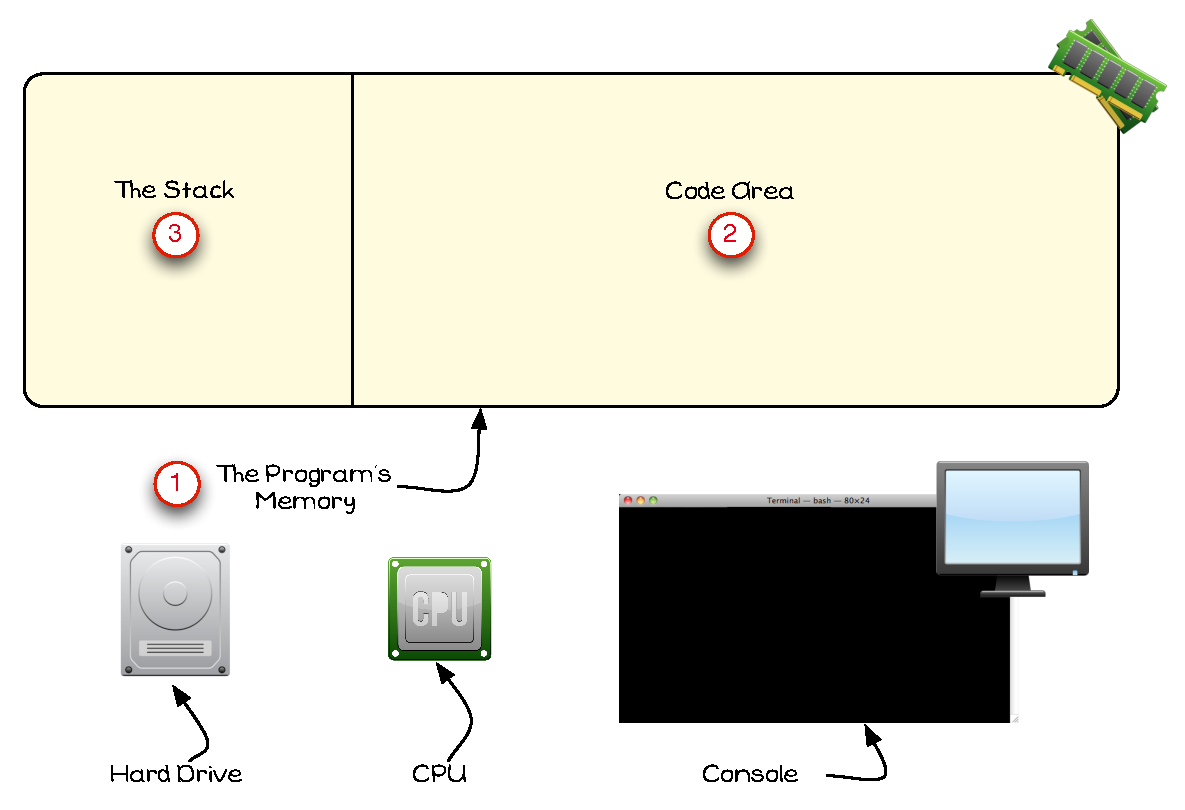
\includegraphics[width=\textwidth]{./topics/program-creation/images/ProgramExecution01} 
   \caption[Program Memory Space]{Operating System prepares memory for the Program}
   \label{fig:program-creation-visualise-helloworld-1}
\end{figure}

\mynote{
\begin{itemize}
  \item In Figure \ref{fig:program-creation-visualise-helloworld-1} the indicated areas show the following:
  \begin{enumerate}
    \item The Operating System allocates memory for the program.
    \item Part of the allocated memory will be designated to store the program's instructions. This can be thought of as the \emph{Code Area}.
    \item Another part of the allocated memory will be set aside to keep track of the current instruction. This area is called the \emph{Stack}.
  \end{enumerate}
\end{itemize}
}

% subsubsection allocating_memory_for_the_program (end)
\clearpage
\subsubsection{Loading the Code} % (fold)
\label{ssub:loading_the_code}

Having allocated the program some memory, and partitioned this space into the \textbf{Stack} and \textbf{Code} area, the Operating System then reads the program's instructions from the executable file and loads these into the Code area. This is illustrated in Figure \ref{fig:program-creation-visualise-helloworld-2}.

\begin{figure}[htbp]
   \centering
   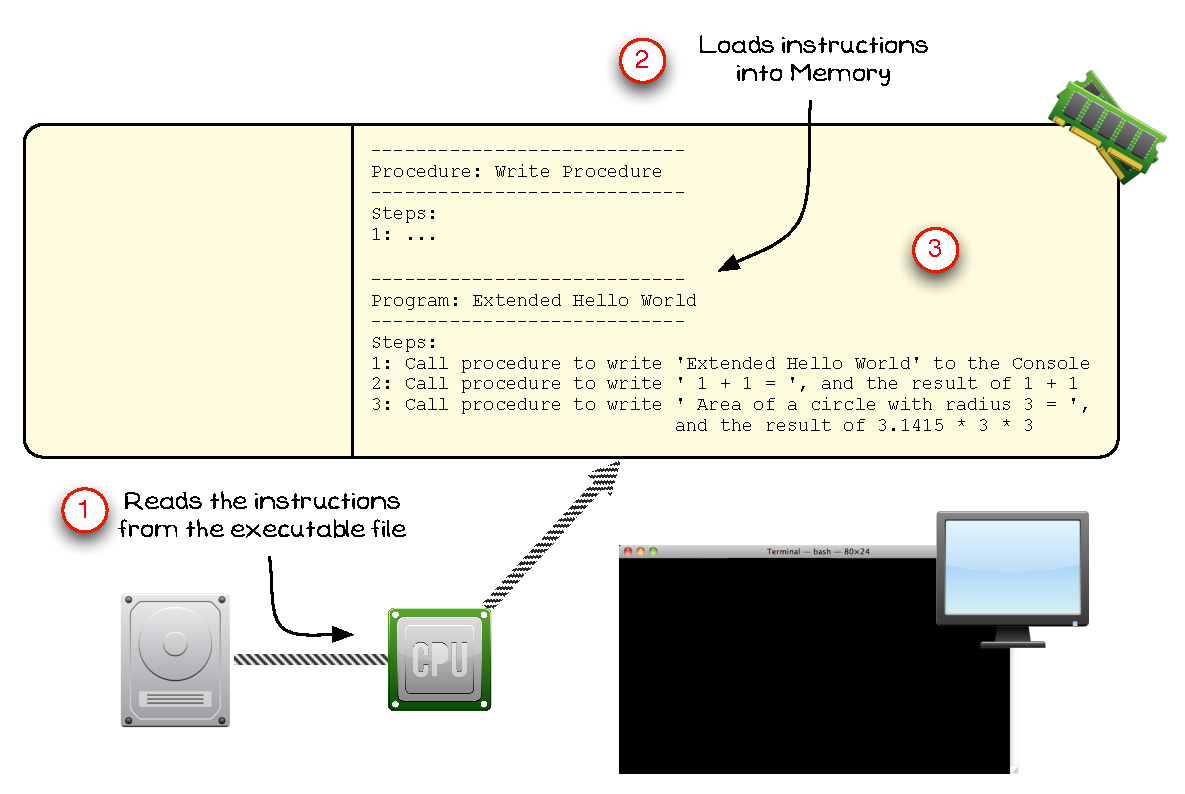
\includegraphics[width=\textwidth]{./topics/program-creation/images/ProgramExecution02} 
   \caption[Code loaded into memory]{The Operating System loads the program's code into memory}
   \label{fig:program-creation-visualise-helloworld-2}
\end{figure}

\mynote {
\begin{itemize}
  \item In Figure \ref{fig:program-creation-visualise-helloworld-2} the indicated areas show the following:
  \begin{enumerate}
    \item The program's instructions are read from the executable file the user launched.
    \item The instructions are stored into the program's memory: into the code area.
    \item When this finishes, all of the program's instructions are loaded into memory. In Figure \ref{fig:program-creation-visualise-helloworld-2} the instructions are shown as the pseudocode from Listing \ref{lst:program-creation-hello-pseudo}. In reality these will be the \emph{machine code} instructions that were saved into the executable file by the compiler.
  \end{enumerate}
  \bigskip
  \item The \emph{Operating System} is a software component that is used to control access to the hardware. In this case the Operating System takes the responsibility for setting up the machine so that it can run the program the user launched.
\end{itemize}
}
% subsubsection loading_the_code (end)

\clearpage
\subsubsection{Setting Up The First Instruction} % (fold)
\label{ssub:setting_up_the_first_instruction}

Now that the code is loaded into memory, the Operating System uses the details saved in the executable file to setup the program's first instruction. This will be loaded onto the Stack, which is responsible for keeping track of the current instruction. The compiler will have used the program's \textbf{entry point} to store these details when the program was compiled. This is shown in Figure \ref{fig:program-creation-visualise-helloworld-3}.

\begin{figure}[htbp]
   \centering
   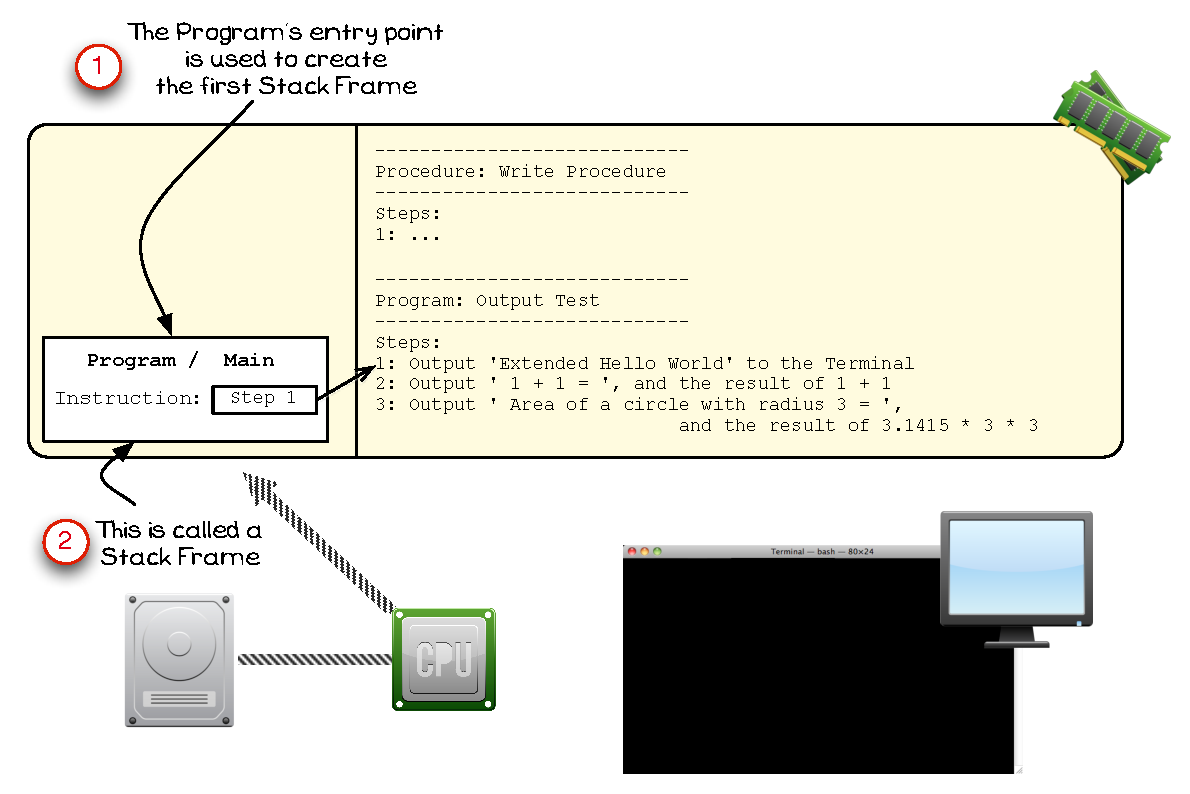
\includegraphics[width=\textwidth]{./topics/program-creation/images/ProgramExecution03} 
   \caption{The current instruction is loaded onto the Stack}
   \label{fig:program-creation-visualise-helloworld-3}
\end{figure}

\mynote {
\begin{itemize}
  \item In Figure \ref{fig:program-creation-visualise-helloworld-3} the indicated areas show the following:
  \begin{enumerate}
    \item The program's instruction is tracked on \emph{The Stack}.
    \item Each Stack Frame keeps a record of the current instruction within a Procedure. This area is called the Stack as the Frames are \emph{stacked} one on top of the other. The one on the top of the \emph{stack} tells the computer which instruction is to be run.
  \end{enumerate}
  \bigskip
  
  \item The Stack keeps track of the current instruction.
  \item The current instruction refers to the code loaded into the Code area.
  \item The compiler will have saved the details for which instruction is first into the executable file.
  \item In your code the program's \textbf{entry point} tells you which instruction will be first.
\end{itemize}
}

% subsubsection setting_up_the_first_instruction (end)

\clearpage
\subsubsection{Running The First Instruction} % (fold)
\label{ssub:running_the_first_instruction}

The Operating System has finally finished loaded the Program, and can now start its instructions running. The CPU uses the \textbf{Current Instruction} that is on the top of the Stack, locates the Code, and runs the instruction. In this case this is a procedure call to a Procedure that writes output to the Terminal. When this instruction completes, the text \emph{Output Test Program} will have appeared on the Terminal for the user to see. The results of this are shown in Figure \ref{fig:program-creation-visualise-helloworld-4}. 

\begin{figure}[htbp]
   \centering
   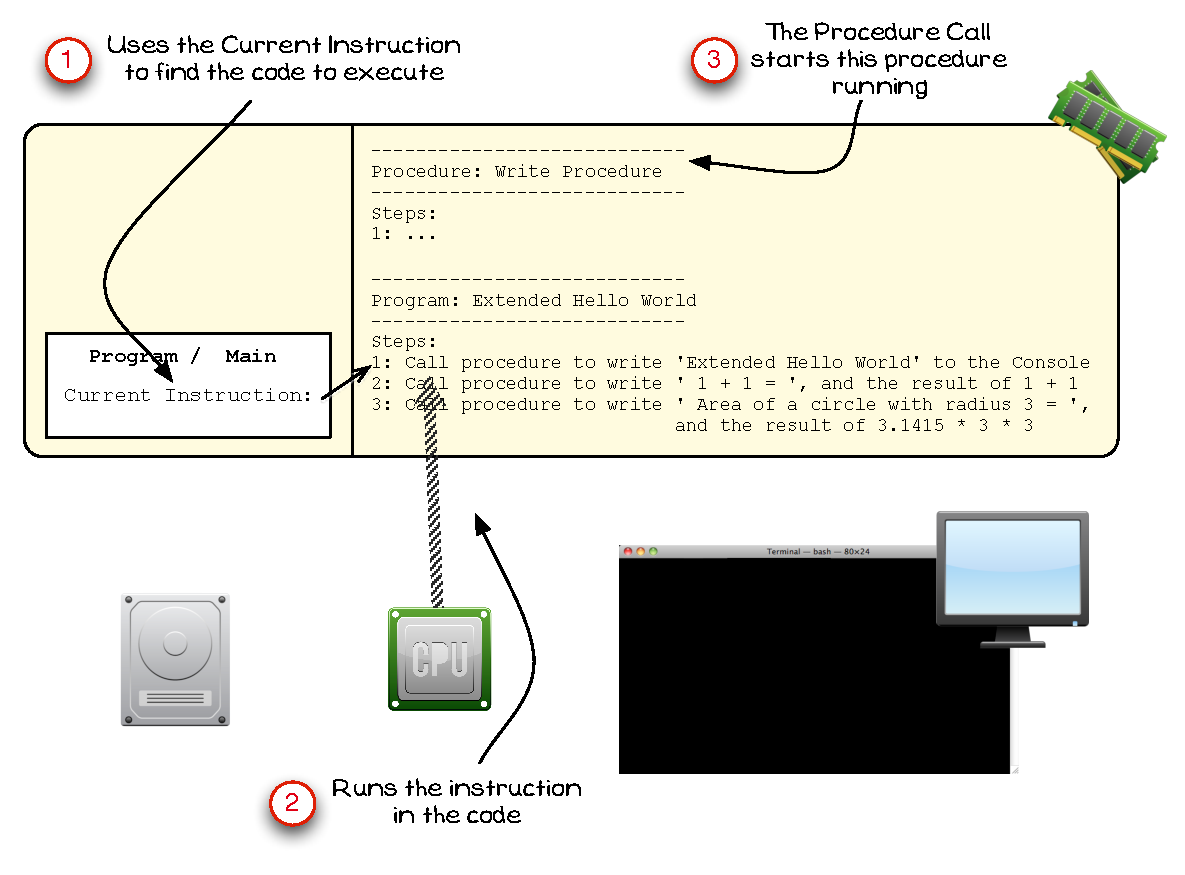
\includegraphics[width=\textwidth]{./topics/program-creation/images/ProgramExecution04} 
   \caption{The Computer runs the first instruction, outputting details to the Terminal}
   \label{fig:program-creation-visualise-helloworld-4}
\end{figure}


\mynote{
\begin{itemize}
  \item In Figure \ref{fig:program-creation-visualise-helloworld-4} the indicated areas show the following:
  \begin{enumerate}
    \item The current instruction is read from the Frame on the top of the Stack.
    \item The Computer runs the instruction from the code loaded into memory.
    \item The instruction is a procedure call, which starts the execution of the Write Procedure.
  \end{enumerate}
  
  \bigskip
  \item The computer runs the code \textbf{one} instruction at a time.
  \item When that instruction is finished it moves onto the next instruction. This is important, and means that are programs run the commands in \textbf{Sequence}.
  \item Writing data to the Terminal takes more than a single instruction, the procedure call gets the Computer to run the instructions in the called Procedure.
\end{itemize}
}

% subsubsection running_the_first_instruction (end)
% subsection starting_a_program (end)

\clearpage
\subsection{Calling the Write Procedure} % (fold)
\label{sub:calling_a_procedure}

At this point the Computer has been instructed to \texttt{Call the Write Procedure}. This procedure\footnote{The \texttt{printf} procedure in C and the \texttt{WriteLn} procedure in Pascal.} will output the data passed to it to the Terminal. In order to do this, the instructions within the called procedure need to be followed.

\subsubsection{Calling Write for the first time} % (fold)
\label{ssub:calling_write_for_the_first_time}

Each Procedure contains instructions that when followed get the Computer to perform a task. The procedure call sets up the Stack so that the instructions within the Write Procedure are executed.

\begin{figure}[htbp]
   \centering
   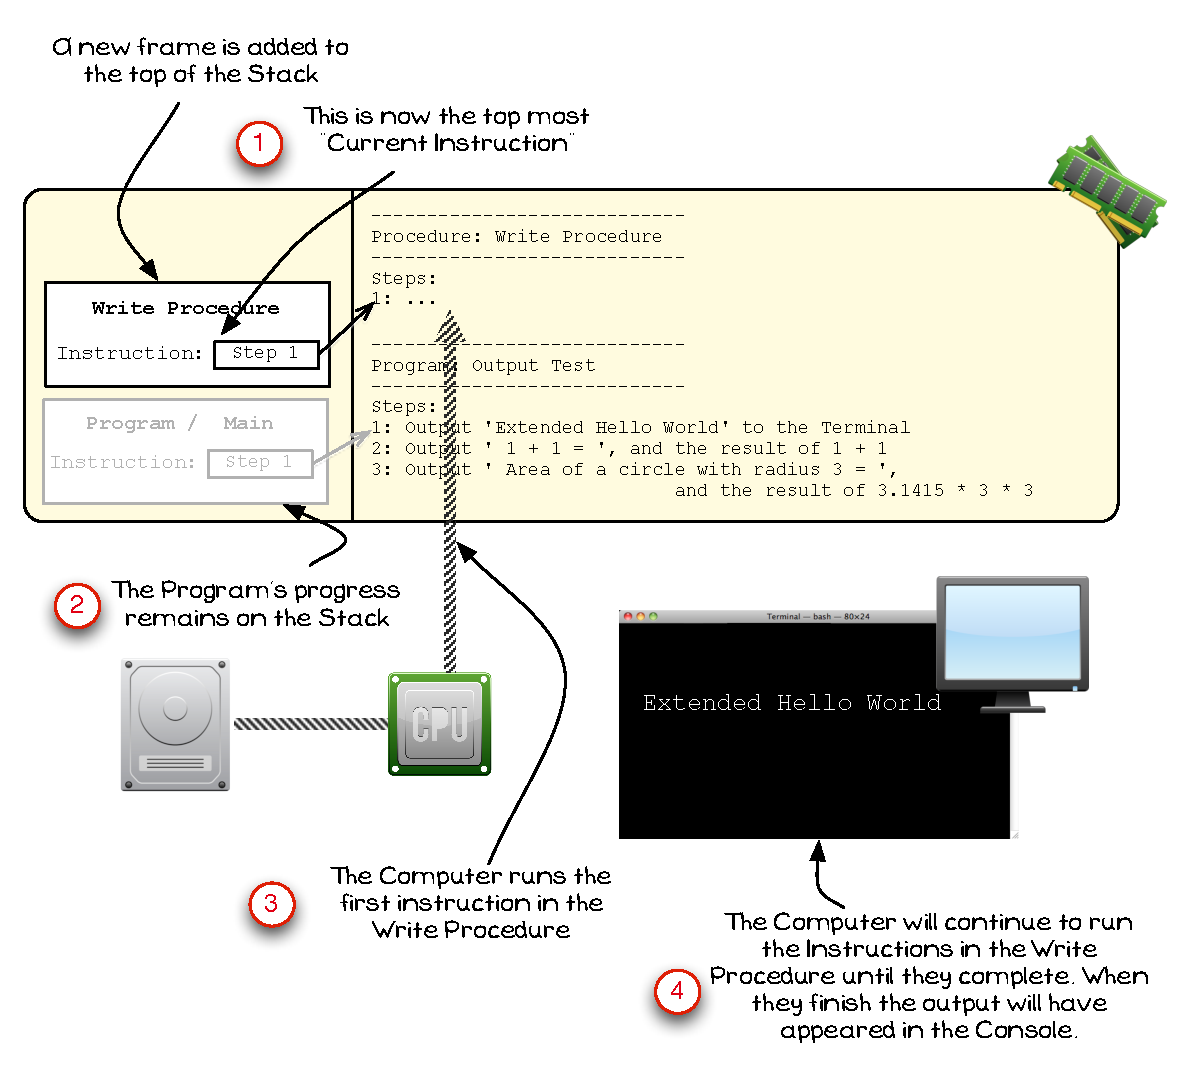
\includegraphics[width=0.9\textwidth]{./topics/program-creation/images/ProgramExecution05} 
   \caption{The Write Procedure is called, and has its instructions executed}
   \label{fig:program-creation-visualise-helloworld-5}
\end{figure}

\mynote{
\begin{itemize}
  \item In Figure \ref{fig:program-creation-visualise-helloworld-5} the indicated areas show the following:
  \begin{enumerate}
    \item A new Frame is added to the Stack for the Write Procedure.
    \item The new Frame appears on top of the Frame that has the program's Current Instruction.
    \item Now the Computer can run the instructions within the Write Procedure.
    \item The instructions are run one at a time until the Write Procedure finishes. At this time the first output will have appeared on the Terminal.
  \end{enumerate}
\end{itemize}
}


% subsubsection calling_write_for_the_first_time (end)
\clearpage
\subsubsection{The Write Procedure Ends} % (fold)
\label{ssub:the_write_procedure_ends}

When the Write Procedure's instructions finish control needs to return to the code that called it, in this case the program's code.

\begin{figure}[htbp]
   \centering
   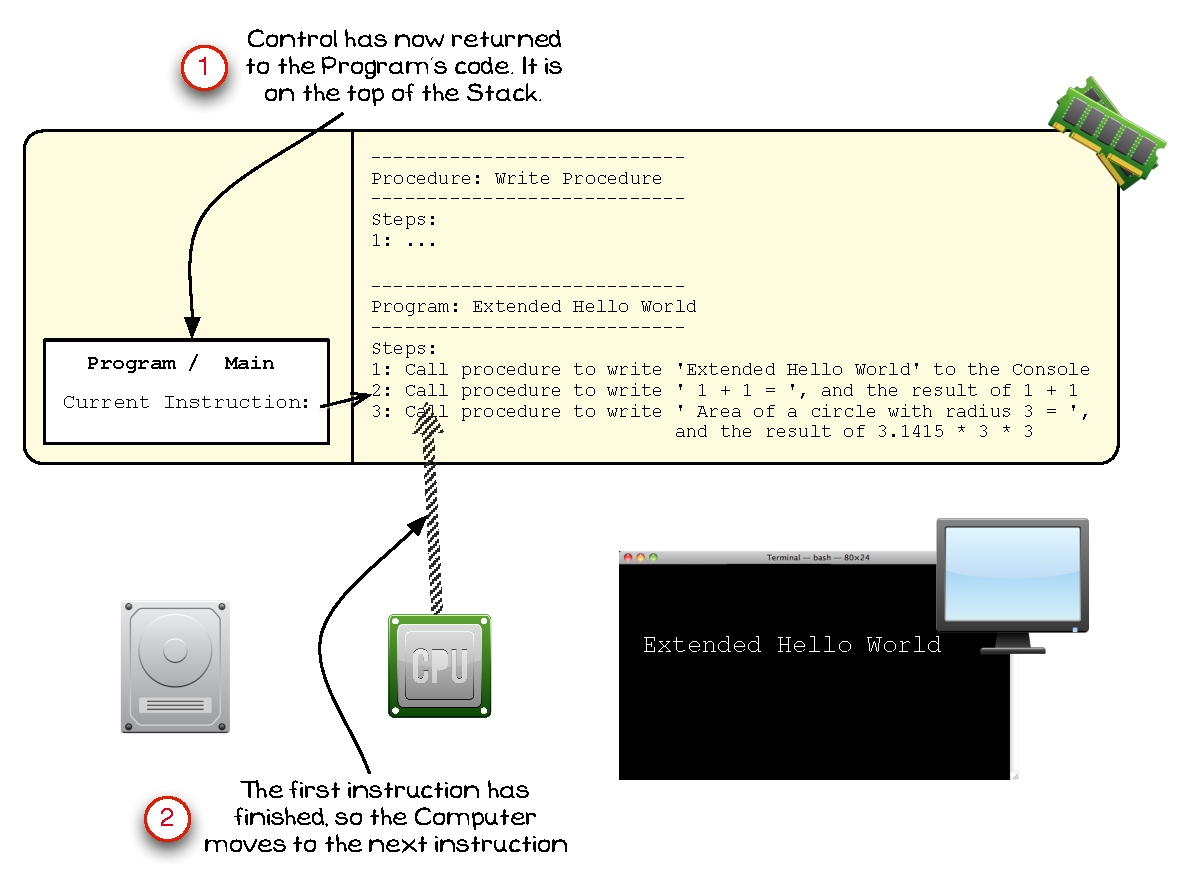
\includegraphics[width=\textwidth]{./topics/program-creation/images/ProgramExecution06} 
   \caption{The Write Procedure is called, and has its instructions executed}
   \label{fig:program-creation-visualise-helloworld-6}
\end{figure}

\mynote{
\begin{itemize}
  \item In Figure \ref{fig:program-creation-visualise-helloworld-6} the indicated areas show the following:
  \begin{enumerate}
    \item When the Write Procedure finishes its Frame is removed from the Stack, and control returns to the program's code.
    \item The first instruction on the program's code has now finished, so the Computer moves to the second instruction.
  \end{enumerate}
\end{itemize}
}

One way to visualise this is to picture the Program, and the Procedure, as a book of instructions. Imagine you are told to follow the instructions in a book. You get the book, place it on a table and read the first instruction which tells you to perform the \emph{Write Procedure}. You leave the original book on the table, and fetch the \emph{Write Procedure} book and place it on top of the book on the table, thereby creating a Stack of books. Now you can follow the instructions, one by one, from the book on top of the Stack. When you finish the last instruction you take the book off the top of the stack and return to the book beneath it. This will enable you to perform the steps within the Procedures without forgetting where you are up to in the earlier code.


% subsubsection the_write_procedure_ends (end)
\clearpage
\subsubsection{The Second Call to Write} % (fold)
\label{ssub:the_second_call_to_write}

The second instruction in the program's code is another call to the Write procedure.

\begin{figure}[htbp]
   \centering
   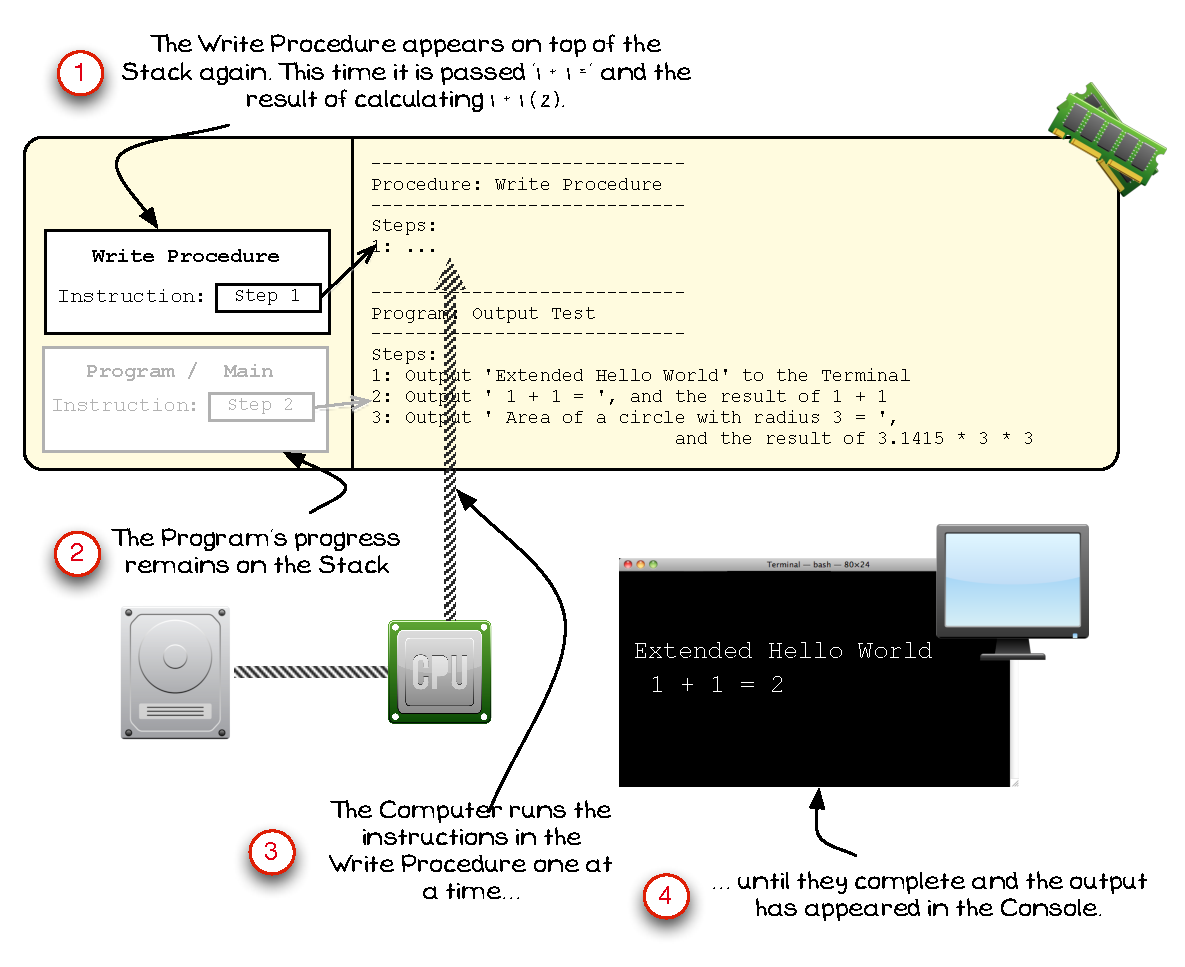
\includegraphics[width=\textwidth]{./topics/program-creation/images/ProgramExecution07} 
   \caption{The Write Procedure is called a second time}
   \label{fig:program-creation-visualise-helloworld-7}
\end{figure}

\mynote{
\begin{itemize}
  \item In Figure \ref{fig:program-creation-visualise-helloworld-7} the indicated areas show the following:
  \begin{enumerate}
    \item A new Frame is created for the Write Procedure. This allows the Computer to keep track of which statement is the current statement within this Procedure.
    \item The program's current instruction remains on the Stack for when the call to the Write procedure finishes.
    \item Each of the instructions in the Write procedure are executed to write the data to the Terminal.
    \item The output text appears on the Terminal.
  \end{enumerate}
\end{itemize}
}

% subsubsection the_second_call_to_write (end)
\clearpage
\subsubsection{The Second Write Call Ends} % (fold)
\label{ssub:the_second_write_call_ends}

When the second call to Write ends control returns to the Program, which moves on to its final instruction.

\begin{figure}[htbp]
   \centering
   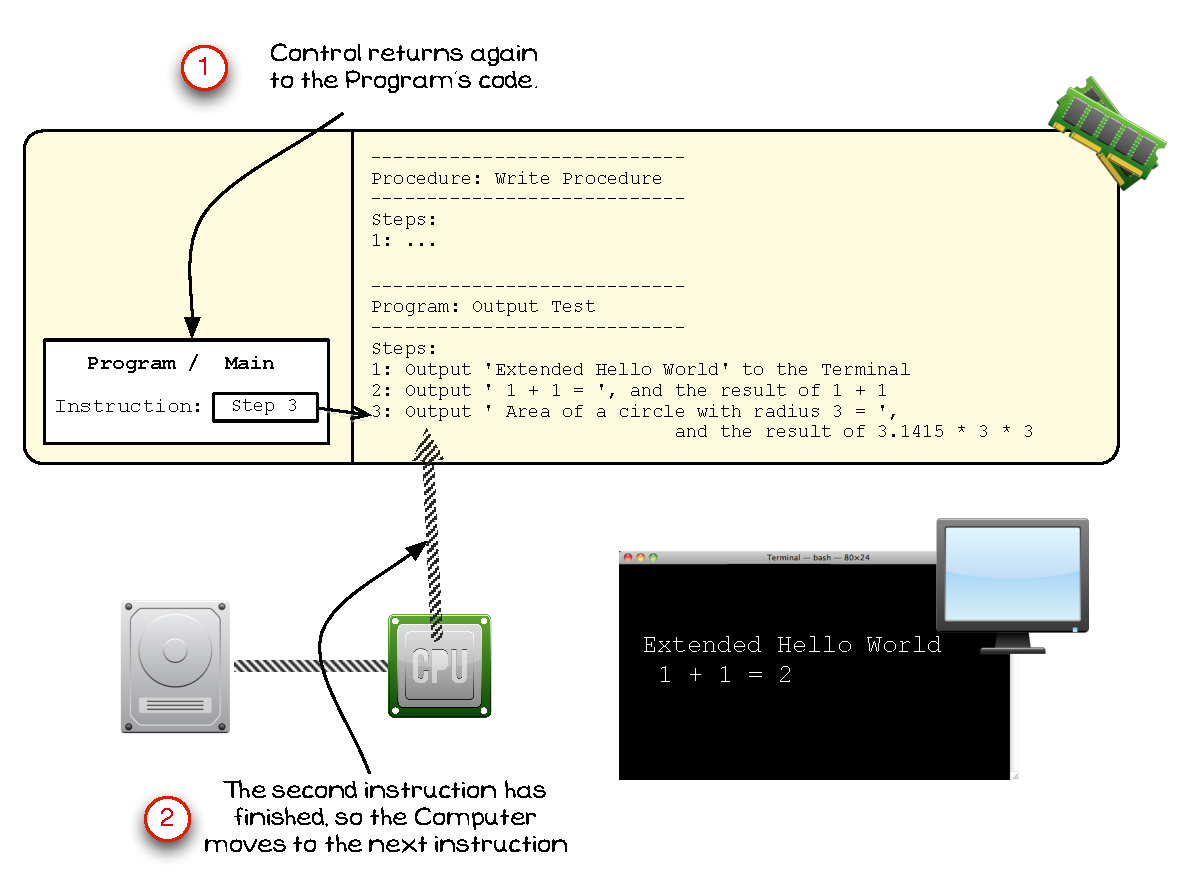
\includegraphics[width=\textwidth]{./topics/program-creation/images/ProgramExecution08} 
   \caption{The second call to the Write Procedure ends, and control returns to the Program}
   \label{fig:program-creation-visualise-helloworld-8}
\end{figure}

\mynote{
\begin{itemize}
  \item In Figure \ref{fig:program-creation-visualise-helloworld-8} the indicated areas show the following:
  \begin{enumerate}
    \item When the second call to the Write Procedure ends control returns to the program's code.
    \item As the second instruction has now finished the Computer moves to the third, and final, instruction in the program.
  \end{enumerate}
\end{itemize}
}

% subsubsection the_second_write_call_ends (end)
\clearpage
\subsubsection{The Third Call to Write} % (fold)
\label{ssub:third_call_to_write}

The final instruction in the program is a third call to the Write Procedure. 

\begin{figure}[htbp]
   \centering
   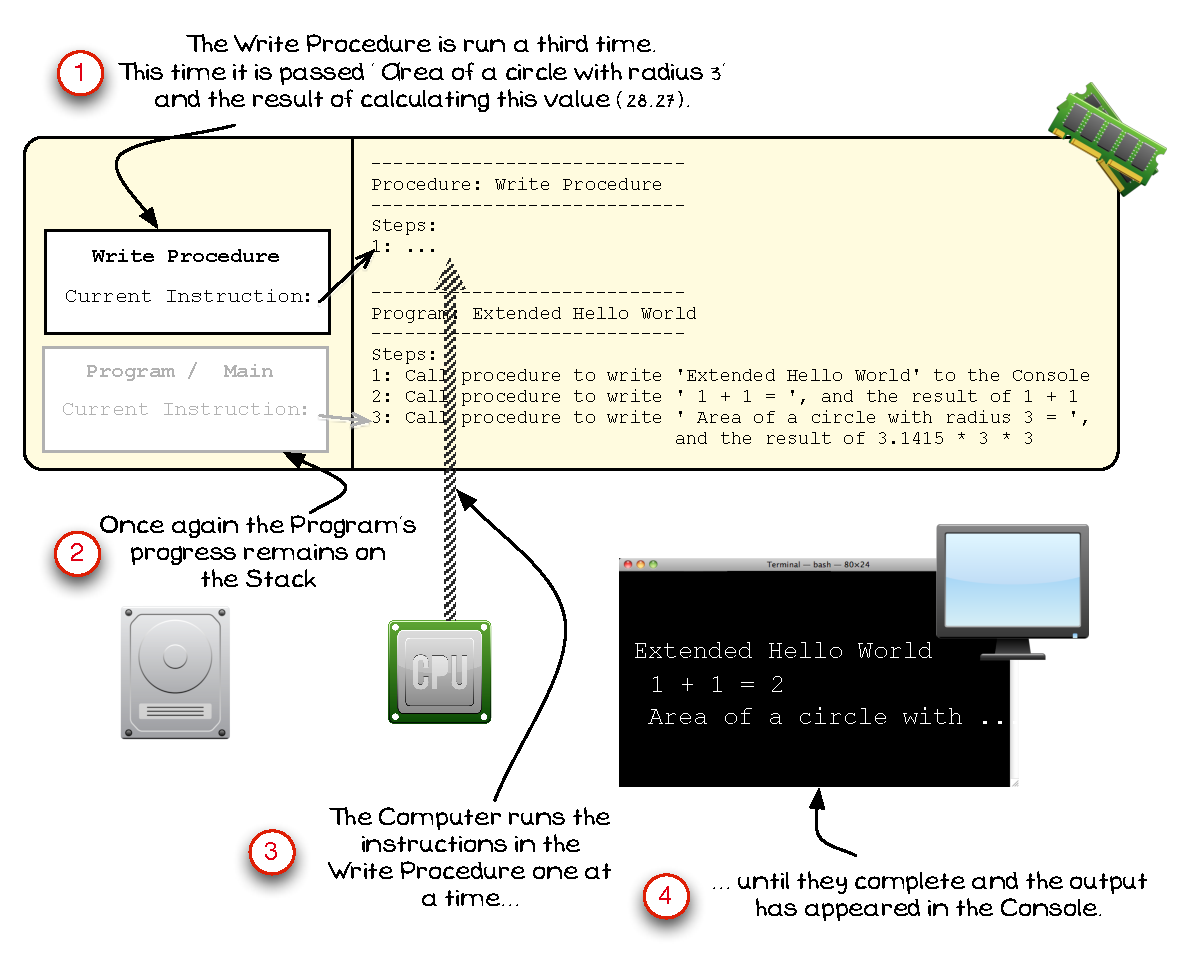
\includegraphics[width=\textwidth]{./topics/program-creation/images/ProgramExecution09} 
   \caption{The Write Procedure is called a third can final time}
   \label{fig:program-creation-visualise-helloworld-9}
\end{figure}

\mynote{
\begin{itemize}
  \item In Figure \ref{fig:program-creation-visualise-helloworld-9} the indicated areas show the following:
  \begin{enumerate}
    \item Once again, a Stack Frame is created to keep track of the progress within the Write Procedure.
    \item The program's current instruction remains on the Stack so that the Computer can return to it when the Write Procedure ends.
    \item Each of the instructions in the Write Procedure are executed.
    \item The Write Procedure writes the data passed to it to the Terminal.
  \end{enumerate}
\end{itemize}
}

% subsubsection third_call_to_write (end)
\clearpage
\subsubsection{The Program Ends} % (fold)
\label{ssub:program_ends}

When the last instruction in the Write Procedure finishes control return back to the Program, which has no more instructions. This means that the program has finished.

\begin{figure}[htbp]
   \centering
   \includegraphics[width=\textwidth]{./topics/program-creation/images/ProgramExecution10} 
   \caption{The Write Procedure ends, then the program ends}
   \label{fig:program-creation-visualise-helloworld-10}
\end{figure}

\mynote{
\begin{itemize}
  \item In Figure \ref{fig:program-creation-visualise-helloworld-10} the indicated areas show the following:
  \begin{enumerate}
    \item The Write Procedure has finished its instructions, and so it ends. This was also the last instruction in the program's code, so it also ends. This tells the Operating System that Program has finished.
    \item The Operating System releases the memory used by the program so that it can be use by other programs.
    \item All of this will have happened in an instant, and after the program has finished all that remains is the output in the Terminal.
  \end{enumerate}
\end{itemize}
}

% subsubsection program_ends (end)

% subsection calling_a_procedure (end)
\clearpage
\subsection{Summary} % (fold)
\label{sub:program_creation_visualise_summary}

In this section you have seen the actions that occur behind the scenes when your program is executed. The most important aspects are the fact that the instructions run one at a time in \textbf{sequence}, and that a procedure call results in the instructions within the Procedure running until they end. Its also important to remember that the instructions within the Procedure must finish before control returns to where the call was made.

\bigskip

\mynote{
\begin{itemize}
  \item A Program is a sequence of instructions.
  \item These instructions are organised into Procedures that can be called. 
  \item The program's instructions are loaded into memory when the program is launched.
  \item Instructions are run one at a time.
  \item The Stack is used to keep track of the current instruction.
  \item When the program starts a Frame is added to the Stack to set the entry point as the first instruction.
  \item When a Procedure is called, a Frame is added to the Stack to keep track of its current instruction. 
\end{itemize}
}

% subsection summary (end)

% section understanding_program_execution (end)

% ====================
% = Examples Section =
% ====================
\clearpage
\section{Program Creation Examples} % (fold)
\label{sec:program_creation_examples}

\subsection{Seven Times Table} % (fold)
\label{sub:seven_times_table}

This program prints out the seven times table from 1 x 7 to 10 x 7. The description of the program is in Table \ref{tbl:program-creation-times-table}, the pseudocode in Listing \ref{lst:program-creation-seven-times-pseudo}, the C code in Listing \ref{lst:program-creation-seven-times-c}, and the Pascal code in Listing \ref{lst:program-creation-seven-times-pas}.

\begin{table}[h]
\centering
\begin{tabular}{l|p{10cm}}
  \hline
  \multicolumn{2}{c}{\textbf{Program Description}} \\
  \hline
  \textbf{Name} & \emph{Seven Times Table} \\
  \\
  \textbf{Description} & Displays the Seven Times Table from 1 x 7 to 10 x 7. \\
  \hline
\end{tabular}
\caption{Description of the Seven Times Table program}
\label{tbl:program-creation-times-table}
\end{table}

\pseudocode{lst:program-creation-seven-times-pseudo}{Pseudocode for Seven Times Table program.}{./topics/program-creation/examples/seven-times.txt}

\clearpage

\csection{\ccode{lst:program-creation-seven-times-c}{C Seven Times Table}{topics/program-creation/examples/seven_times.c}}
\passection{\pascode{lst:program-creation-seven-times-pas}{Pascal Seven Times Table}{topics/program-creation/examples/SevenTimesTable.pas}}

% subsection times_table (end)
\clearpage
\subsection{Circle Area} % (fold)
\label{sub:circle_area}

This program prints out the area of circles with different radius. The description of the program is in Table \ref{tbl:program-creation-circle-area}, the pseudocode in Listing \ref{lst:program-creation-circle-areas-pseudo}, the C code in Listing \ref{lst:program-creation-circle-areas-c}, and the Pascal code in Listing \ref{lst:program-creation-circle-areas-pas}.

\begin{table}[h]
\centering
\begin{tabular}{l|p{10cm}}
  \hline
  \multicolumn{2}{c}{\textbf{Program Description}} \\
  \hline
  \textbf{Name} & \emph{Circle Areas} \\
  \\
  \textbf{Description} & Displays the Circle Areas for circles with radius from 1.0 to 5.0 with increments of 0.5. \\
  \hline
\end{tabular}
\caption{Description of the Circle Areas program}
\label{tbl:program-creation-circle-area}
\end{table}

\pseudocode{lst:program-creation-circle-areas-pseudo}{Pseudocode for Circle Area program.}{./topics/program-creation/examples/circle_areas.txt}

\clearpage

\csection{\ccode{lst:program-creation-circle-areas-c}{C Circle Areas}{topics/program-creation/examples/circle_areas.c}}
\passection{\pascode{lst:program-creation-circle-areas-pas}{Pascal Circle Areas}{topics/program-creation/examples/CircleAreas.pas}}

% subsection circle_area (end)
\clearpage
\subsection{Shape Drawing} % (fold)
\label{sub:shape_drawing}

This program draws some shapes to the screen using the \textbf{SwinGame} Software Development Kit (SDK). The SwinGame SDK is a library that provides a number of reusable code artefacts that you can use to create 2D games. This SDK is available for both C and Pascal, and work on Linux, Mac, and Windows.

The description of the program is in Table \ref{tbl:program-creation-shape-drawing}, the pseudocode in Listing \ref{lst:program-creation-shape-drawing-pseudo}, the C code in Listing \ref{lst:program-creation-shape-drawing-c}, and the Pascal code in Listing \ref{lst:program-creation-shape-drawing-pas}.

\begin{table}[h]
\centering
\begin{tabular}{l|p{10cm}}
  \hline
  \multicolumn{2}{c}{\textbf{Program Description}} \\
  \hline
  \textbf{Name} & \emph{Shape Drawing} \\
  \\
  \textbf{Description} & Draws a number of shapes to the screen using SwinGame. \\
  \hline
\end{tabular}
\caption{Description of the Shape Drawing program}
\label{tbl:program-creation-shape-drawing}
\end{table}

\pseudocode{lst:program-creation-shape-drawing-pseudo}{Pseudocode for Shape Drawing program.}{./topics/program-creation/examples/shape_drawing.txt}

The Lines from the program will do the following:
\begin{itemize}
  \item \textbf{\texttt{OpenGraphicsWindow}} opens a Window with the title `Shape Drawing' that is 800 pixels wide by 600 pixels high.
  \item \textbf{\texttt{ClearScreen}} clears the screen to black.
  \item \textbf{\texttt{FillRectangle}} uses the color, the x, y location, and width and height to fill a rectangle.
  \item \textbf{\texttt{RefreshScreen}} updates the screen to show what has been drawn. All SwinGame drawing is done offscreen, and only drawn to the screen when RefreshScreen is called.
  \item \textbf{\texttt{Delay}} pauses the program for a number of milliseconds, so 500 will wait for half a second.
  \item \textbf{\texttt{FillCircle}} uses the color, given x, y location and radius to fill a circle.
  \item \textbf{\texttt{FillTriangle}} fills a triangle with the given x, y points (6 values for 3 points).
\end{itemize}

\clearpage

\csection{\ccode{lst:program-creation-shape-drawing-c}{C Shape Drawing Code}{topics/program-creation/examples/shape_drawing.c}}

The SwinGame procedure for C are named using the standard C naming scheme. The names are:
\begin{itemize}
  \item \textbf{\texttt{open\_graphics\_window}} opens a Window with the title `Shape Drawing' that is 800 pixels wide by 600 pixels high.
  \item \textbf{\texttt{load\_default\_colors}} loads default colors for use in your code.
  \item \textbf{\texttt{clear\_screen}} clears the screen to black.
  \item \textbf{\texttt{fill\_rectangle}} uses the color, the x, y location, and width and height to fill a rectangle.
  \item \textbf{\texttt{refresh\_screen}} updates the screen to show what has been drawn. All SwinGame drawing is done offscreen, and only drawn to the screen when RefreshScreen is called.
  \item \textbf{\texttt{delay}} pauses the program for a number of milliseconds, so 500 will wait for half a second.
  \item \textbf{\texttt{fill\_circle}} uses the color, given x, y location and radius to fill a circle.
  \item \textbf{\texttt{fill\_triangle}} fills a triangle with the given x, y points (6 values for 3 points).
\end{itemize}


\clearpage

\passection{\pascode{lst:program-creation-shape-drawing-pas}{Pascal Shape Drawing Code}{topics/program-creation/examples/ShapeDrawing.pas}}


% subsection shape_drawing (end)

% section program_creation_examples (end)

% =============
% = Exercises =
% =============
\clearpage
\section{Program Creation Exercises} % (fold)
\label{sec:program_creation_exercises}

\begin{enumerate}
  \item Write a program that prints the 73 times table from 1 * 73 to 10 * 73.
  \begin{itemize}
    \item Draw up a outline of the program
    \item Write pseudocode for the program's instructions
    \item Convert your pseudocode to either C or Pascal
    \item Compile and Run your program, and check that the values are correctly calculated
  \end{itemize}
  
  \item Write a program that prints the powers\footnote{In the code you will need to calculate these manually using times ($2^1$ = 2, $2^2$ = 2*2, $2^3$ = 2*2*2, etc.)} of 2 from $2^1$ to $2^8$.
  \begin{itemize}
    \item Draw up a outline of the program
    \item Write pseudocode for the program's instructions
    \item Convert your pseudocode to either C or Pascal
    \item Compile and Run your program, and check that the values are correctly calculated
  \end{itemize}
  
  
  \item Write a program that prints a table that shows calculations related to circles. This should output the  radius, circle area, diameter, and circumference.
  \begin{itemize}
    \item Find the necessary calculations and then draw up a outline of the program
    \item Write pseudocode for the program's instructions
    \item Convert your pseudocode to either C or Pascal
    \item Compile and Run your program, and check that the values are correctly calculated
  \end{itemize}
  
  \item Write a program that draws a face on the screen using SwinGame.
  \begin{itemize}
    \item Draw up an outline of the program. Work out the coordinates of the circles for the face, circles. Determine three points of the triangle for the mouth.
    \item Write up the pseudocode for the program's instructions. Remember to use the \texttt{RefreshScreen} and \texttt{Delay} procedures to see the results.
    \item Convert your pseudocode to either C or Pascal
    \item Compile and Run your program, and check that the values are correctly calculated
  \end{itemize}
\end{enumerate}

% section program_creation_exercises (end)

% ===================
% = Project Section =
% ===================
\clearpage
\section{Program Creation Project} % (fold)
\label{sec:program_creation_project}

% section program_creation_project (end)

% chapter program_creation (end)
  % \chapter{Procedure Declaration} % (fold)
\label{cha:procedure_declaration}

\begin{quote}
  \Fontlukas\Large
  \renewcommand{\LettrineTextFont}{\relax}
  \lettrine[image=true,lines=3,lraise=0.1]
  {Y}{our} spell casting is really coming along. As you know, your spells contain a sequence of incantations. I will now teach you a technique to combine incantations into groups. This will make your spells faster to cast, and easier to use. Now get your wand, and try casting your spell like this\ldots
\end{quote}

\bigskip

Programs contain a sequence of instructions, with each instruction \emph{commanding} the computer to perform an action. While it is possible to have just a single long list of instructions, this quickly becomes difficult to understand, hard to extend, and frustrating to maintain. Rather than coding all of a program's instructions in a single list, Software Developers arrange a program's instructions in meaningful groups that can be called when those steps need to be performed. These groups are called \emph{Procedures}. Within a Program, each Procedure is designed to get the computer to perform a single task, and therefore only contains the instructions related to that task.

When you have understood the material in this chapter you will be able to create and call simple Procedures of your own creation. This will help make your programs faster and easier to write.

\minitoc

% ====================
% = Concepts Section =
% ====================

\clearpage
\section{Procedure Declaration Concepts} % (fold)
\label{sec:procedure_declaration_concepts}

Chapter \ref{cha:program_creation} \nameref{cha:program_creation} introduced the idea of creating your own Programs as a sequence of instructions, \nameref{sub:statement}s. The instructions in these programs called existing \nameref{sub:procedure}s that performed tasks for the program. The code you wrote sequenced these procedures to produce a desired output.

As you learnt in Chapter \ref{cha:program_creation}, \nameref{sub:procedure}s are designed to perform a single task that can be called when you want that task performed. Using Procedures from Libraries is an important task, but what about the tasks related to the program we are creating? Can we create our own procedures that help us to model the actions we want performed in the code?

The simple answer is \emph{yes}. Yes you can, and should, create your own procedures. These procedures enable you to model the processes related to your program, capturing the individual tasks in the Procedures your create. 

In this Chapter you will learn how to create the following programming \textbf{artefacts}:

\begin{itemize}
  \item \nameref{sub:program_with_procedures_}: Lets you create Procedures in your program's code.
  \item \nameref{sub:proc_decl-procedure_declarations}: Declare the actions the Procedure will perform.
\end{itemize}

\bigskip

You may need to revise the following programming terminology:
\begin{itemize}
  \item \nameref{sub:statement}: An instruction performed in your code.
  \item \nameref{sub:identifier}: The name of an artefact, or the text used to identify something meaningful to the language.
\end{itemize}

This material also requires that you have a good understanding of the following actions:
\begin{itemize}
  \item \nameref{sub:procedure call}: A procedure call is an instruction to run a Procedure.
\end{itemize}

By the end of this material we will have worked through an example where you create a program that writes a small Morse Code message to the Terminal. This program will break the functionality across a number of procedures, making it easy to extend to output other messages. The output of the program is shown in Figure \ref{fig:procedure-decl-morse_calling}.

\begin{figure}[h]
   \centering
   \includegraphics[width=0.9\textwidth]{./topics/program-creation/images/MorseCalling} 
   \caption{Morse Calling run in the Terminal}
   \label{fig:procedure-decl-morse_calling}
\end{figure}


\clearpage
\subsection{Program (with Procedures)} % (fold)
\label{sub:program_with_procedures_}

Each Program is a list of instructions (\nameref{sub:statement}s) that command the computer to perform actions. Unfortunately the computer is only able to perform simple actions, meaning that even small programs need many instructions in order to perform their tasks. To help manage these instructions you can group the program's Statements into Procedures, creating Procedures that perform the tasks you need completed in your Program.

\begin{figure}[h]
   \centering
   \includegraphics[width=\textwidth]{./topics/program-creation/diagrams/ProgramWithProc} 
   \caption{Program with Procedures}
   \label{fig:procedure-decl-program}
\end{figure}

\mynote{
\begin{itemize}
  \item A Program is an \textbf{artefact} that you can \emph{create} in your code.
  \item A Program can contain a number of \nameref{sub:procedure}s.
  \item \nameref{sub:proc_decl-procedure_declarations} allow you to create your own Procedures.
  \item The program's instructions can call the Procedures you create in the program's code.
  \item In C and Pascal the \nameref{sub:proc_decl-procedure_declarations} must appear before they are used in your code.
\end{itemize}
}

% subsection program_with_procedures_ (end)
\clearpage
\subsection{Procedure Declarations} % (fold)
\label{sub:proc_decl-procedure_declarations}

Procedures contain code that define the steps the computer performs when the procedure is called. In your Program you can define your own Procedures, allowing you to divide a program's tasks into separate Procedures.

\begin{figure}[h]
   \centering
   \includegraphics[width=\textwidth]{./topics/program-creation/diagrams/ProcedureDeclaration} 
   \caption{Procedure Declaration}
   \label{fig:procedure-decl-procedure-decl}
\end{figure}

\mynote{
\begin{itemize}
  \item A Procedure is an \textbf{artefact} that you can \emph{create} and \emph{use} in your code.
  \item Each Procedure contains code to perform a certain task. When you want the task performed you call the Procedure.
  \item Procedures should have a \textbf{side effect}\footnote{Output to the Terminal is an example of a Side Effect. After calling these procedures the text you wanted to appear was written to the Terminal. These Procedures changed the Terminal.}, meaning that it changes something when it is executed.
  \item The Procedure's declaration defines its \textbf{name}, and the \textbf{steps} it performs.
  \item Each instructions in the Procedure is a \nameref{sub:statement}.
  \item The Procedure's \nameref{sub:identifier}:
  \begin{itemize}
    \item Is the name used to call the Procedure.
    \item Should be a \textbf{verb} that \textbf{reflects the task} the Procedure performs.
  \end{itemize} 
  \item When the Procedure is called its instructions are executed.
  \item Each Procedure's instructions are isolated from the other code in your Program. When you are working on a Procedure you do not need to know about the internal workings of the other procedures.
\end{itemize}
}

% subsection procedure_declarations (end)

\clearpage
\subsection{Summary} % (fold)
\label{sub:procedure-decl_summary}

This section has introduced you to the idea of creating and using your own Procedures. The concepts related to this are shown in Figure \ref{fig:procedure-decl-summary}. The next section will examine how these concepts can be used to design the Morse Code program.

\begin{figure}[h]
   \centering
   \includegraphics[width=\textwidth]{./topics/program-creation/diagrams/Summary} 
   \caption[Chapter Concepts]{Key Concepts introduced in this Chapter}
   \label{fig:procedure-decl-summary}
\end{figure}

\mynote{
\begin{itemize}
  \item \textbf{Artefacts} are things you can \emph{create} and \emph{use}.
  \item \textbf{Terms} are things you need to \emph{understand}.
  \item \textbf{Actions} are things you can \emph{command} the computer to perform.
\end{itemize}
}


% subsection summary (end)


% section procedure_declaration_concepts (end)


% ========================
% = Using these concepts =
% ========================

\clearpage
\section{Using these Concepts} % (fold)
\label{sec:using_these_concepts_procedure_decl}

Procedures give us a means of modelling the tasks we want the computer to perform. Rather than just having a long list of instructions, we can create procedures that contain the steps needed to perform individual tasks that the program must carry out. The program's instructions can then be very simple, just calling the procedures that we have written to carry out the tasks as needed.

\subsection{Designing Morse Calling} % (fold)
\label{sub:designing_morse_calling}

Table \ref{tbl:procedure-decl-morse_calling} contains a description of the next program we are going to design. This program will output a message in Morse Code to the Terminal. In designing this program we will make use of the concepts introduced in this chapter; we will divide the program's code into a number of procedures each with the instructions to get the computer to perform a single task.

\begin{table}[h]
\centering
\begin{tabular}{l|p{10cm}}
  \hline
  \multicolumn{2}{c}{\textbf{Program Description}} \\
  \hline
  \textbf{Name} & \emph{Morse Calling} \\
  \\
  \textbf{Description} & Displays the morse code for `\emph{Calling Anyone}' on the Terminal. \\
  \hline
\end{tabular}
\caption{Description of the Morse Calling program.}
\label{tbl:procedure-decl-morse_calling}
\end{table}

To design and implement this program we need to follow a number of steps:
\begin{enumerate}
  \item Understand the problem, and get some ideas on the tasks that need to be performed.
  \item Choose the artefacts we will create and use
  \item Map these artefacts to code
  \item Compile and run the program
\end{enumerate}

Our first step will be to analyse the problem, and find related material that we can use to make sure we know what the computer needs to do. You need to understand what the program needs to do before you can design the solution. For this program you need to find out a little more about Morse Code so that you can issue the right signals. An important part of this analysis will be to identify the tasks that need to performed in order to meet the programs requirements.

Having understood the problem, the next step will be to create a design for the solution. This involves choosing the artefacts (procedures at this point) that you will \textbf{use}, and the artefacts that you will \textbf{create}. You use the information you gained from analysing the requirements to help you model the tasks that need to be performed in the code.

This is the point where you need to map the artefacts that you need to create to code. You can use the Language Syntax rules to determine what needs to be typed in order to make sure your program will compile.

Finally you can test your program by running it and observing the output. If there are compiler errors then you need to fix these, so that the program compiles. Then you need to check that the output of the program matches the expected outcome. Your understanding of how the program should work will be important during the testing as much as it was during the design and implementation.

\clearpage
\subsection{Understanding Morse Calling} % (fold)
\label{ssub:understanding_morse_calling}

Understanding the problem is the first step toward creating a solution. In this case you need to understand Morse Code so that you can work out what needs to be written to the Terminal. Wikipedia describes Morse Code as a sequence of long and short signals used to encode textual data. When we write this out to the Terminal the short signals can be represented using a dot (.), the long signals using a dash (-). Table \ref{tbl:procedure-decl-morse-codes} contains the Morse code signals for letters, numbers, and some punctuation.

\begin{table}[htbp]
  \centering
  \begin{tabular}{|p{1cm}l|p{1cm}l|p{1cm}l|p{1cm}l|}
    \hline
    \centering A & {\huge \morse a}  & \centering K & {\huge \morse K} & \centering U & {\huge \morse U} & \centering 4 & {\huge \morse 4}\\
    \centering B & {\huge \morse b}  & \centering L & {\huge \morse L} & \centering V & {\huge \morse V} & \centering 5 & {\huge \morse 5}\\
    \centering C & {\huge \morse c}  & \centering M & {\huge \morse M} & \centering W & {\huge \morse W} & \centering 6 & {\huge \morse 6}\\
    \centering D & {\huge \morse d}  & \centering N & {\huge \morse N} & \centering X & {\huge \morse X} & \centering 7 & {\huge \morse 7}\\
    \centering E & {\huge \morse e}  & \centering O & {\huge \morse O} & \centering Y & {\huge \morse Y} & \centering 8 & {\huge \morse 8}\\
    \centering F & {\huge \morse f}  & \centering P & {\huge \morse P} & \centering Z & {\huge \morse Z} & \centering 9 & {\huge \morse 9}\\
    \centering G & {\huge \morse g}  & \centering Q & {\huge \morse Q} & \centering 0 & {\huge \morse 0} & \centering . & {\huge \morse .}\\
    \centering H & {\huge \morse h}  & \centering R & {\huge \morse R} & \centering 1 & {\huge \morse 1} & \centering , & {\huge \morse ,}\\
    \centering I & {\huge \morse i}  & \centering S & {\huge \morse S} & \centering 2 & {\huge \morse 2} & \centering ? & {\huge \morse ?}\\
    \centering J & {\huge \morse j}  & \centering T & {\huge \morse T} & \centering 3 & {\huge \morse 3} & \centering ! & {\huge \morse !}\\
    \hline
  \end{tabular}
  \caption{Morse code signals for letters and numbers}
  \label{tbl:procedure-decl-morse-codes}
\end{table}

With some additional searching you can also find that the signal for `\emph{Calling Anyone}' is the code to signal C and Q. This means that the Program needs to output the signals {\morse CQ} (the signals for C and Q), see Table \ref{tbl:procedure-decl-morse-codes}.

\bigskip

As you read through this information its important to try and identify the tasks that the program will need to perform. These tasks can then be modelled in the program's code. The following list outlines the tasks that can be identified in the above descriptions. Read back over the text and make sure you can see where each of these can be identified.

\begin{itemize}
  \item Perform a Short Signal (a dot)
  \item Perform a Long Signal (a dash)
  \item Signal the Character C
  \item Signal the Character Q
\end{itemize}

When you design the solution for this program you will be able to use this information to determine what needs to be created, and the tasks that each of these performs.

\begin{itemize}
  \item Perform Short Signal will output a dot (.) to the Terminal.
  \item Perform Long Signal will output a dash (-) to the Terminal.
  \item Signal C will perform a Long Signal, then a Short Signal, then a second Long Signal, and a second Short Signal. This will end by printing a space to separate it from the next character.
  \item Signal Q will perform a Long Signal, a second Long Signal, a Short Signal, and then a third Long Signal. This will end by printing a space to separate it from the next character.
\end{itemize}

% subsubsection understanding_morse_calling (end)
\clearpage
\subsection{Choosing Artefacts for Morse Calling} % (fold)
\label{sub:procedure-decl-choosing_artefacts}

Having finished the analysis of the problem, the next step is to design the solution. This will involve determining which programming artefacts you will need to build, and the which programming artefacts exist for you to use. 

\begin{itemize}
  \item Create a \textbf{program} the user can execute. This will signal C and Q using Morse Code. Within this program there are several sub-tasks that can be coded into their own procedures.
  \begin{itemize}
    \item \textbf{Short Signal} - Morse Code needed the ability to perform a short signal. The instructions for this can be coded into a \emph{Short Signal} procedure. In this case that will output a dot (.) to the Terminal.
    \item \textbf{Long Signal} - Similar to the \emph{Short Signal}, this procedure will contain the instructions needed to perform a \emph{Long Signal}, in this case this will output a dash (-) to the Terminal.
    \item \textbf{Signal C} - This task will contain the instructions needed to get the computer to signal the character C. Internally this can call the \emph{Short Signal} and \emph{Long Signal} procedures.
    \item \textbf{Signal Q} - Similar to the \emph{Signal C}, this procedure will contain the instructions needed to signal the character Q. Internally it will use the \emph{Short Signal} and \emph{Long Signal} procedures.
  \end{itemize}
  \item The following procedures already exist and can be used to help implement the procedures mentioned above:
  \begin{itemize}
    \item The language provides a procedure to write data to the Terminal.
  \end{itemize}
\end{itemize}

\csection{In C the procedure to write data to the Terminal is the \texttt{printf} procedure from \texttt{stdio.h}.}
\passection{In Pascal there are two procedures to write data to the Terminal, \texttt{Write} and \texttt{WriteLn}.}

The pseudocode for the \emph{Morse Calling} program is shown in Listing \ref{lst:procedure-decl-MorseCalling-pseudo}, with pseudocode for the \emph{Signal C} procedure in Listing \ref{lst:procedure-decl-signalc-pseudo}, \emph{Signal Q} in Listing \ref{lst:procedure-decl-signalq-pseudo}, and Listing \ref{lst:procedure-decl-shortsignal-pseudo} showing the pseudocode for the \emph{Short Signal} procedure.

\clearpage
\pseudocode{lst:procedure-decl-MorseCalling-pseudo}{Pseudocode for Morse Calling program.}{./topics/procedure-decl/application/MorseCalling.txt}

\pseudocode{lst:procedure-decl-signalc-pseudo}{Pseudocode for the Signal C procedure.}{./topics/procedure-decl/application/SignalC.txt}

\pseudocode{lst:procedure-decl-signalq-pseudo}{Pseudocode for the Signal Q procedure.}{./topics/procedure-decl/application/SignalQ.txt}

\pseudocode{lst:procedure-decl-shortsignal-pseudo}{Pseudocode for the Short Signal procedure.}{./topics/procedure-decl/application/ShortSignal.txt}

\pseudocode{lst:procedure-decl-longsignal-pseudo}{Pseudocode for the Long Signal procedure.}{./topics/procedure-decl/application/LongSignal.txt}

\mynote{
Have a look over the Procedures and the Morse Calling Program and note the following things:
\begin{itemize}
  \item The Procedures appear within the Program.
  \item The name of the procedure indicates what it does.
  \item \texttt{Short Signal} is called by the \texttt{Signal C} and \texttt{Signal Q} procedures.
  \item \texttt{Short Signal} is not directly called by the Program.
  \item The \texttt{SignalC} Procedure calls the \texttt{Long Signal} and \texttt{Short Signal} procedures.
  \item In the C or Pascal code, the Procedure's declaration must appear before its use, so \texttt{Short Signal} and \texttt{Long Signal} will need to appear at the top of the code, \texttt{Signal C} and \texttt{Signal Q} in the middle, and the Program's instructions at the end.
\end{itemize}
}

% subsection choosing_artefacts (end)

\clearpage
\subsection{Writing the Code for Morse Calling} % (fold)
\label{sub:writing_the_code_for_morse_calling}

The pseudocode from section \ref{sub:procedure-decl-choosing_artefacts} \nameref{sub:procedure-decl-choosing_artefacts} shows the instructions, and how these should be divided between a number of custom created procedures. At this stage these instructions need to be translated into source code, so that they can be compiled and the resulting program tested.

The following two sections, Section \ref{sec:procedure_declaration_in_c} \nameref{sec:procedure_declaration_in_c} and Section \ref{sec:procedure_declaration_in_pascal} \nameref{sec:procedure_declaration_in_pascal}, contain a description of the syntax needed to create programs in the C and Pascal programming languages that include Procedure declarations.

Each of these sections will contain extended Program declaration rules that show you where the Procedure Declarations can be coded, along with the rules for how Procedure Declarations should appear.

\mynote{

Remember the basic process for reading the Syntax Diagrams is to:
\begin{enumerate}
  \item Find the page with the Syntax rule you are interested in knowing about.
  \item Have a quick look at the Syntax Diagram and the rules it contains. Read each rule, and get a basic feel for how it is going to come together for your program.
  \item Read the example to see one way of using the Rule. The Syntax Diagram can be used to create any number of variations of the rule, the example gives you at least one way these rules can be coded.
  \item Return to the diagram and make sure you can match each part of the example back to the rule that created it.
  \item Now look up any related rules that are not explained on this rule's page. For example, a \nameref{sub:program_with_procedures_} uses the \nameref{sub:proc_decl-procedure_declarations} rule, you will need to read this rule to determine how to declare the Procedures you want to create in the code.
\end{enumerate}

}

% subsection writing_the_code_for_morse_calling (end)
\subsection{Compiling and Running Morse Calling} % (fold)
\label{sub:compiling_and_running_morse_calling}

Once you have completed your program, you need to compile and test it. 

\begin{enumerate}
  \item Open the \textbf{Terminal}\footnote{The \textbf{MinGW Shell} on Windows.} program for your Operating System
  \item Use the \texttt{\textbf{cd}} command to move to the directory with your code, for example \newline \bashsnipet{cd /Users/acain/Documents/Code}
  \item Run the compiler with your program's code. See the language specific details below.
  \item Fix any compiler errors, using the tips from Section \ref{ssub:compiler_errors} \nameref{ssub:compiler_errors}.
  \item Execute the program using \bashsnipet{./MorseCalling} and check the results
\end{enumerate}

\csection{
The C compiler is called \textbf{gcc}. To compile your \emph{Morse Calling} program you will need to run the following: \newline \newline \bashsnipet{gcc -o MorseCalling morse-calling.c}
}

\passection{
The Pascal compiler is called \textbf{fpc}. To compile your \emph{Morse Calling} program you will need to run the following: \newline \newline \bashsnipet{fpc -S2 MorseCalling.pas}
}



% subsection compiling_and_running_morse_calling (end)


% subsection designing_morse_calling (end)


% section using_these_concepts (end)

% =============
% = C Section =
% =============

\cleardoublepage
\def\pageLang{c}
\section{Procedure Declarations in C} % (fold)
\label{sec:procedure_declaration_in_c}

% Concept overview
\subsection{Implementing Morse Calling in C} % (fold)
\label{sub:implementing_morse_calling_in_c}

Section \ref{sec:using_these_concepts_procedure_decl} of this chapter introduced the `Morse Calling' program, and its design. Its implementation requires the definition of some procedures in the Program's code. This section of the chapter introduces the C syntax rules for declaring your own procedures, with the C implementation of Morse Calling being shown in Listing \ref{lst:procedure-decl-c-morse_calling}.

\csection{\ccode{lst:procedure-decl-c-morse_calling}{C Morse Calling}{code/c/procedure-decl/morse-calling.c}}

\mynote{
\begin{itemize}
  \item Save the C code in a file named \texttt{morse-calling.c}.
  \item Compile this using \bashsnipet{gcc -o MorseCalling morse-calling.c}.
  \item Run the resulting program using \bashsnipet{./MorseCalling}.
  \item Check that the output matches the expected values.
  \item Looking over the code you should be able to see the instructions for each Procedure.
  \item Notice how the indentation makes it easy to see where each Procedure starts and ends. Always lay your code out so that it is easy to see its structure.
  \item See how the procedures are declared before they are used. This is important as the C compiler must know about the Procedure before you can call it.
  \item To see how to create this have a look at the Syntax for declaring \nameref{sub:c_program_with_procedures_}.
  \item The Program's declaration can contain a number of Procedures using the \nameref{sub:c_procedure_declaration} syntax.
\end{itemize}
}

% subsection implementing_morse_sos_in_c (end)

% Parts of the syntax


% section procedure_declaration_in_c (end)


% ==================
% = Pascal Section =
% ==================

\cleardoublepage
\def\pageLang{pas}
\section{Procedure Declarations in Pascal} % (fold)
\label{sec:procedure_declaration_in_pascal}

% Concept overview
\subsection{Implementing Morse Calling in Pascal} % (fold)
\label{sub:implementing_morse_calling_in_pascal}

Section \ref{sec:using_these_concepts_procedure_decl} of this chapter introduced the `Morse Calling' program, and its design. Its implementation requires the definition of some procedures in the program's code. This section of the chapter introduces the Pascal syntax rules for declaring your own procedures, with the Pascal implementation of Morse Calling being shown in Listing \ref{lst:procedure-decl-pas-morse_calling}.

\passection{\pascode{lst:procedure-decl-pas-morse_calling}{Pascal Morse Calling}{code/pascal/procedure-decl/MorseCalling.pas}}

\mynote{
\begin{itemize}
  \item Save the Pascal code in a file named \texttt{MorseCalling.pas}.
  \item Compile this using \bashsnipet{fpc -S2 MorseCalling.pas}.
  \item Run the resulting program using \bashsnipet{./MorseCalling}.
  \item Check that the output matches the expected values.
  \item Looking over the code you should be able to see the instructions for each procedure.
  \item Notice how the indentation makes it easy to see where each procedure starts and ends. Always lay your code out so that it is easy to see its structure.
  \item See how the procedures are declared before they are used. This is important as the Pascal compiler must know about procedures before you can call them.
  \item To see how to create this have a look at the syntax for declaring \nameref{sub:pas_program_with_procedures_}.
  \item The program's declaration can contain a number of procedures using the \nameref{sub:pas_procedure_declaration} syntax.
\end{itemize}
}

% subsection implementing_morse_sos_in_c (end)

% Parts of the syntax
\clearpage
\subsection{Pascal Program (with Procedures)} % (fold)
\label{sub:pas_program_with_procedures_}

The Pascal code for a program contains the program's instructions, along with your own procedure declarations.

\passyntax{passynt:procedure-decl-program}{a program (with procedures)}{procedure-decl/program-with-procedures}

\passection{\pascode{lst:program-pas-say-hello-proc}{Is Anyone There?}{code/pascal/procedure-decl/SayHelloProc.pas}}

\mynote{
\begin{itemize}
  \item Within your program you can declare your own procedures. 
  \item See \nameref{sub:pas_procedure_declaration} for the syntax to declare your own procedures.
  \item Listing \ref{lst:program-pas-say-hello-proc} shows a program with three procedures: \texttt{Main}, \texttt{ SayHello()}, and \texttt{ SayIsAnyoneThere()}.
  \item Procedures are declared between the \emph{program's header} and the \emph{program's statements}.
\end{itemize}
}



% subsection c_program_with_procedures_ (end)
\clearpage
\subsection{Pascal Procedure Declaration} % (fold)
\label{sub:pas_procedure_declaration}

The syntax for a Pascal procedure declaration is shown in \fref{passynt:procedure-decl-procedure-decl}.

\passyntax{passynt:procedure-decl-procedure-decl}{a procedure}{procedure-decl/procedure-decl}

\passection{\pascode{lst:program-pas-print-steps}{Cooking a meal}{code/pascal/procedure-decl/PrintSteps.pas}}

\mynote{
\begin{itemize}
  \item There are four procedures declared in the code in \lref{lst:program-pas-print-steps}.
  \item A \textbf{procedure declaration} starts with the word \textbf{\texttt{procedure}}. This indicates to the compiler that the following code is a procedure declaration.
  \item The \textbf{procedure's name} is an identifier. This can be any valid \nameref{sub:pas_identifier} that has not been used before.
  \item The empty parenthesis must appear after the procedure's name, and before the semicolon and the \emph{block}.
  \bigskip
  \item There are a number of conventions, called coding standards, that describe how your code should appear for a given language. In this text we will use a common Pascal convention of having all \emph{procedure names} in \textbf{Pascal Case}, this uses an uppercase character for the first letter of each word in the identifier. So the \emph{Get Ingredients} procedure becomes \texttt{GetIngregients}.
\end{itemize}
}

% subsection c_procedure_declaration (end)


% section procedure_declaration_in_c (end)


% =========================
% = Understanding Section =
% =========================
\clearpage
\def\pageLang{none}
\section{Understanding Procedure Declaration and Calls} % (fold)
\label{sec:understanding_procedure_declaration_and_calls}

This Chapter has introduced the idea of creating Procedures within your program's code. These procedures can be used to implement the different tasks that you want your program to perform. 

This Section will help you answer the following questions:
\begin{itemize}
  \item How can I visualise the Procedures within a program?
  \item What happens when my Procedures are called?
\end{itemize}

\subsection{Visualising Procedures in Morse Calling} % (fold)
\label{sub:visualising_morse_calling}

When you are writing the code, the internal details of how a Procedure works are important. But, it is equally important to be able to picture how these procedures interact within the program as a whole. One technique for visualising this is to draw a \textbf{Structure Chart}.

A \emph{Structure Chart} is a diagram that has two elements: rectangles representing the procedures in your code, and arrows representing calls. The Structure Chart for the Morse Calling program is shown in Figure \ref{fig:procedure-decl-morsecalling-structure}. In this you can see that the Morse Calling program has four main procedures that implement its functionality, in addition to the program's main logic: the \texttt{Signal C}, \texttt{Signal Q}, \texttt{Long Signal}, and \texttt{Short Signal} procedures. It also shows that the program's main logic calls \texttt{Signal C} and \texttt{Signal Q}, that \texttt{Signal C} calls \texttt{Long Signal} and \texttt{Short Signal}, as does \texttt{Signal Q}.

\begin{figure}[htbp]
   \centering
   \includegraphics[width=0.75\textwidth]{./topics/program-creation/diagrams/MorseCallingStructureChart} 
   \caption{Structure Chart showing the Procedures in Morse Calling}
   \label{fig:procedure-decl-morsecalling-structure}
\end{figure}

The rectangles in the Structure Chart represent the Procedures. As the name of the procedure should reflect its task/actions this means that the reader of the diagram can get some insight into what the program is doing, and how it is achieving its tasks. From Morse Calling's Structure Chart you can see that the program is Signalling the character's \emph{C} and \emph{Q}, which internally use \emph{Long} and \emph{Short} signals to achieve their tasks.

The arrows in the Structure Chart show procedure calls. The arrow from the \texttt{Signal C} procedure to \texttt{Long Signal} tells us that somewhere in the code for \texttt{Signal C} there is one or more calls to \texttt{Long Signal}. There is no indication of the order, or frequency, of these calls. Its just simply saying that \texttt{Signal C} calls \texttt{Long Signal}.

The Structure Chart is useful for getting an overall picture of how the program is structured. It can help the designer communicate such things as \emph{What Procedures are there in this program?} and \emph{How are these Procedures related to each other?} It helps developers new to the project to get a feeling for how the code is distributed within the solution, and to know where the core logic can be found. It also provides a means of determining the impact of changing the functionality of the tasks in the program. For example, if you change how \texttt{Long Signal} works that may impact on \texttt{Signal C} and on \texttt{Signal Q}. Any changes you made here would mean you needed to test that \texttt{Signal C} and \texttt{Signal Q} still worked as expected.

\bigskip

The Structure Chart is a great communication tool for getting an overall picture of how a solution fits together, but it only shows the \textbf{static structure}. Communicating things about the code, but not things about how the code executed. An effective designer will want to communicate both the \emph{static structure}, as well as the \textbf{dynamic behaviour} of the solution. To communicate these details you need to look for complementary techniques.

% sub:visualising_morse_calling (end)

\subsection{Visualising procedure calls in Morse Calling} % (fold)
\label{sub:visualising_procedure_calls_in_morse_calling}

The Structure Chart communicates the static structure of the solution, showing the Procedures and their relationships but lacking any details on how this structure works dynamically. This dynamic information can be captured in a \textbf{Sequence Diagram}, which works together with the Structure Chart to complete the overview of the program's structure and dynamic behaviour.

Figure \ref{fig:procedure-decl-morsecalling-sequence} shows the \emph{Sequence Diagram} for the Morse Calling program. This shows the \emph{procedure calls} that will occur within an execution of the program's code. The Sequence Diagram shows the order in which procedure calls occur, with time travelling down the page and the calls travelling across. 

\begin{figure}[htbp]
   \centering
   \includegraphics[width=0.75\textwidth]{./topics/program-creation/diagrams/MorseCallingSequenceDiagram} 
   \caption{Sequence Diagram for Morse Calling}
   \label{fig:procedure-decl-morsecalling-sequence}
\end{figure}

You start reading this diagram from the top, with each arrow representing the call to a Procedure, and the thin vertical rectangles representing the time taken for the called procedure to complete its task. Reading the Sequence Diagram for Morse Calling you can see that the first thing to occur is the \texttt{Main} body of the program's code is started. The arrow from the far left indicates that something, in this case being the user launching the program, starts this code running.

The first thin vertical rectangle is the program's main instructions, and its first action is to call \texttt{Signal C} as shown by the arrow pointing to the second vertical bar. This is our first procedure call, the program's instructions call \texttt{Signal C}. Notice that at this point there are two vertical bars. These represent the two frames on the Stack, and show us that when \texttt{Signal C} finishes the execution will return to the program's main instructions.

Within \texttt{Signal C} the first action is to call \texttt{Long Signal}, as shown be the arrow. Time-wise this is the second procedure call. First the Main code called \texttt{Signal C}, which in turn called \texttt{Long Signal}. The details on the diagram show us that \texttt{Long Signal} does not call any other procedures that we created. Notice that we have avoided putting in the call to the output procedure to allow us to focus on the Procedures we have created. At this point there are three frame's on the Stack, the first for the \texttt{Main} code, second for \texttt{Signal C}, and third for \texttt{Long Signal}. You can see these if you turn your head on the side. Notice the notice that the vertical bars will mirror the stack.

As \texttt{Long Signal} does not call any other Procedures that we created there are no calls coming out from this procedure's execution. The actions within this code will be performed, and then \texttt{Long Signal} will end. This is shown by the ending of the vertical bar, and a dashed returning arrow showing where the code returns to. This tells us that when \texttt{Long Signal} ends at this point, the computer returns to execute the next instruction in \texttt{Signal C}.

The next instruction in \texttt{Signal C} is the call to \texttt{Short Signal}. Once again this is shown with the calling arrow, and a vertical bar is added to show the steps of the \texttt{Short Signal} executing. \texttt{Short Signal} does not call any other Procedures we created so it ends without any additional calls occurring, and control returns to \texttt{Signal C}.

This process continues, with the diagram showing that \texttt{Long Signal} is called again followed by a call to \texttt{Short Signal}, and then \texttt{Signal C} ends. At this point control returns to the program's main code, where the next call starts \texttt{Signal Q} running. Within \texttt{Signal Q} you can see two calls to \texttt{Long Signal}, followed by a call to \texttt{Short Signal}, and a final call to \texttt{Long Signal}. When the final call to \texttt{Long Signal} ends this marks the end of the \texttt{Signal Q} procedures, and the end of the program's instructions as a whole.

As you can see from the above text the Sequence Diagram communicates a large amount of detail in a relatively small space. Trying to communicate the calling sequence in words is far harder than doing so in a diagram like this. The Sequence Digram allows software designers to communicate the dynamic behaviour of a software solution.

One issue with a Sequence Diagram is that it can quickly become very large if you use it to try and explain all of the actions within a program. As the complexity of your programs grow you will see that it becomes more and more difficult to try to communicate all of the program's behaviour in a single diagram. Instead of trying to communicate the entire program's behaviour, effective Software Designers will use Sequence Diagrams to communicate important details that may be missed otherwise. Focusing on areas where the interaction between the procedures is particularly important. As you progress as a Software Developer see if you can use these diagrams to effectively communicate important points in your designs.

\bigskip

Together \emph{Structure Charts} and \emph{Sequence Diagrams} allow Software Designers to communicate the static structure and dynamic behaviour of their designs. As a software developer you will need to understand how to read these diagrams, and use them to communicate your designs decisions.

% subsection visualising_procedure_calls_in_morse_calling (end)

\subsection{procedure calls in Action} % (fold)
\label{sub:procedure_calls_in_action}

The Sequence Diagram gives you a way of visualising what happens at run time, but let us return to our virtual computer and see how these actions actually work within the computer. 

\begin{enumerate}
  \item \nameref{ssub:morse_calling_is_loaded_into_memory}
  \item \nameref{ssub:signal_c_is_called}
  \item \nameref{ssub:long_signal_is_called}
  \item \nameref{ssub:control_returns_to_signal_c}
  \item \nameref{ssub:short_signal_is_called}
  \item \nameref{ssub:short_signal_ends}
\end{enumerate}

\clearpage
\subsubsection{Morse Calling is Loaded into Memory} % (fold)
\label{ssub:morse_calling_is_loaded_into_memory}

When the program is launched the Operating System loads the code for Morse Calling into memory, and starts it executing in the program's entry point. 

\begin{figure}[htbp]
   \centering
   \includegraphics[width=\textwidth]{./topics/program-creation/images/ProcExe1} 
   \caption{The Operating System loads the code for Morse Calling into memory}
   \label{fig:procedure-decl-visualise-morsecalling-1}
\end{figure}

\mynote{
\begin{itemize}
  \item In Figure \ref{fig:procedure-decl-visualise-morsecalling-1} the indicated areas show the following:
  \begin{enumerate}
    \item The Operating System reads the code from the Morse Calling executable.
    \item This code is then loaded into the program's memory.
    \item A frame is added to the Stack for the entry point, the start of the program's instructions.
  \end{enumerate}
  \bigskip
  
  \item The memory for the program is divided into areas for the \textbf{stack}, and the \textbf{code}.
  \item Only part of the program's code is shown in Figure \ref{fig:procedure-decl-visualise-morsecalling-1}, but in reality all of the program's code is loaded into memory.
\end{itemize}
}

% subsubsection morse_calling_is_loaded_into_memory (end)

\clearpage
\subsubsection{Signal C is Called} % (fold)
\label{ssub:signal_c_is_called}

The first action in the program's code is a procedure call that starts the code in \texttt{Signal C} running. 

\begin{figure}[htbp]
   \centering
   \includegraphics[width=\textwidth]{./topics/program-creation/images/ProcExe2} 
   \caption{The first instruction calls \texttt{Signal C}}
   \label{fig:procedure-decl-visualise-morsecalling-2}
\end{figure}

\mynote{
\begin{itemize}
  \item In Figure \ref{fig:procedure-decl-visualise-morsecalling-2} the indicated areas show the following:
  \begin{enumerate}
    \item The first instruction in the program's is a call to \texttt{Signal C}.
    \item When this is executed a frame is added to the Stack to keep track of the current instruction within \texttt{Signal C}'s code.
    \item As \texttt{Signal C} is now on top of the Stack its instructions are executed. The first instruction in \texttt{Signal C} is a call to \texttt{Long Signal}.
  \end{enumerate}
  \bigskip
  
  \item Notice that the previous Stack Frame keeps track of where the instructions return when \texttt{Signal C} finishes.
  \item The computer runs each instruction one at a time, using the stack to remember where to return when the current Procedure ends.
\end{itemize}
}


% subsubsection signal_c_is_called (end)

\clearpage
\subsubsection{Long Signal is Called} % (fold)
\label{ssub:long_signal_is_called}

The first action in \texttt{Signal C} is to call \texttt{Long Signal}.

\begin{figure}[htbp]
   \centering
   \includegraphics[width=\textwidth]{./topics/program-creation/images/ProcExe3} 
   \caption{Within \texttt{Signal C} the first instruction is to call \texttt{Long Signal}}
   \label{fig:procedure-decl-visualise-morsecalling-3}
\end{figure}

\mynote{
\begin{itemize}
  \item In Figure \ref{fig:procedure-decl-visualise-morsecalling-3} the indicated areas show the following:
  \begin{enumerate}
    \item The first instruction in the \texttt{Signal C} is a call to \texttt{Long Signal}.
    \item When this is executed a frame is added to the Stack to keep track of the current instruction within \texttt{Long Signal}'s code.
    \item As \texttt{Long Signal} is now on top of the Stack its instructions are executed.
  \end{enumerate}
  \bigskip
  
  \item Notice that the previous Stack Frames remain on the Stack to keep track of where the instructions return when \texttt{Long Signal} and \texttt{Signal C} finish.
  \item The computer runs each instruction one at a time, using the stack to remember where to return when the current Procedure ends.
  \item If you look at the Stack you can see that \texttt{Main} called \texttt{Signal C} that called \texttt{Long Signal}. Flip back and have a look at the \nameref{fig:procedure-decl-morsecalling-sequence}, notice that the arrows at the start of the diagram match the current state of the Stack.
\end{itemize}
}

% subsubsection long_signal_is_called (end)

\clearpage
\subsubsection{Control Returns to Signal C} % (fold)
\label{ssub:control_returns_to_signal_c}

When \texttt{Long Signal} finishes running, it has written an underscore to the Terminal, and control returns back to \texttt{Signal C}.

\begin{figure}[htbp]
   \centering
   \includegraphics[width=\textwidth]{./topics/program-creation/images/ProcExe4} 
   \caption{\texttt{Long Signal}'s instructions end, returning control to \texttt{Signal C}}
   \label{fig:procedure-decl-visualise-morsecalling-4}
\end{figure}

\mynote{
\begin{itemize}
  \item In Figure \ref{fig:procedure-decl-visualise-morsecalling-4} the indicated areas show the following:
  \begin{enumerate}
    \item The computer runs the instructions in \texttt{Long Signal} until they end.
    \item \texttt{Long Signal} has the \textbf{side effect} of writing an underscore to the Terminal.
    \item When \texttt{Long Signal}'s instructions end control returns to \texttt{Signal C}.
    \item The computer now advanced to the next instruction in \texttt{Signal C}.
  \end{enumerate}
  \bigskip
  
  \item Procedures should have side effects, changing something as a result of being called.
  \item \texttt{Signal C} is now at its second instruction as the computer has finished its first instruction.
  \item In the \nameref{fig:procedure-decl-morsecalling-sequence} the program is now at the point after the first returning\footnote{The dashed arrow returned back from \texttt{Long Signal}.} arrow and is now about to call \texttt{Short Signal}.
\end{itemize}
}


% subsubsection control_returns_to_signal_c (end)

\clearpage
\subsubsection{Short Signal is Called} % (fold)
\label{ssub:short_signal_is_called}

The second action in \texttt{Signal C} is to call \texttt{Short Signal}.

\begin{figure}[htbp]
   \centering
   \includegraphics[width=\textwidth]{./topics/program-creation/images/ProcExe5} 
   \caption{\texttt{Short Signal} is called}
   \label{fig:procedure-decl-visualise-morsecalling-5}
\end{figure}

\mynote{
\begin{itemize}
  \item In Figure \ref{fig:procedure-decl-visualise-morsecalling-5} the indicated areas show the following:
  \begin{enumerate}
    \item The second instruction in the \texttt{Signal C} is a call to \texttt{Short Signal}.
    \item When this is executed a frame is added to the Stack to keep track of the current instruction within \texttt{Short Signal}'s code.
    \item As \texttt{Short Signal} is now on top of the Stack its instructions are executed.
  \end{enumerate}
  \bigskip
  
  \item In the \nameref{fig:procedure-decl-morsecalling-sequence} the program is now in the call to \texttt{Short Signal}.
\end{itemize}
}

% subsubsection short_signal_is_called (end)

\clearpage
\subsubsection{Short Signal Ends} % (fold)
\label{ssub:short_signal_ends}

When \texttt{Short Signal} ends control returns again to \texttt{Signal C}, with \texttt{Short Signal} having output a . to the Terminal.

\begin{figure}[htbp]
   \centering
   \includegraphics[width=\textwidth]{./topics/program-creation/images/ProcExe6} 
   \caption{\texttt{Short Signal} ends, returning control to \texttt{Signal C} again}
   \label{fig:procedure-decl-visualise-morsecalling-6}
\end{figure}

\mynote{
\begin{itemize}
  \item In Figure \ref{fig:procedure-decl-visualise-morsecalling-6} the indicated areas show the following:
  \begin{enumerate}
    \item The computer runs the instructions in \texttt{Short Signal} until they end.
    \item \texttt{Short Signal} has the \textbf{side effect} of writing an dot to the Terminal.
    \item When \texttt{Short Signal}'s instructions end control returns to \texttt{Signal C}.
    \item The computer now advanced to the next instruction in \texttt{Signal C}, the third Statement in the code.
  \end{enumerate}
\end{itemize}
}

% subsubsection short_signal_ends (end)

\clearpage
\subsubsection{Signal C runs to completion} % (fold)
\label{ssub:signal_c_runs_to_completion}

\texttt{Signal C} continues to run until it reaches the end of its instructions.

\begin{figure}[htbp]
   \centering
   \includegraphics[width=\textwidth]{./topics/program-creation/images/ProcExe7} 
   \caption{\texttt{Signal C} runs until its instructions end}
   \label{fig:procedure-decl-visualise-morsecalling-7}
\end{figure}

\mynote{
\begin{itemize}
  \item In Figure \ref{fig:procedure-decl-visualise-morsecalling-7} the indicated areas show the following:
  \begin{enumerate}
    \item Each instruction in \texttt{Signal C} is run until all of the instructions in \texttt{Signal C} are complete.
    \item The side effects of the calls to \texttt{Long Signal} and \texttt{Short Signal} can be seen in the Terminal.
    \item The final state of the Terminal, showing {\morse C}, shows the side effect of calling \texttt{Signal C}.
  \end{enumerate}
\end{itemize}
}

% subsubsection signal_c_runs_to_completion (end)

\clearpage
\subsubsection{Signal Q is Called} % (fold)
\label{ssub:signal_q_is_called}

When \texttt{Signal C} finished the computer returns to the program's main instructions, where it moves on to the call to \texttt{Signal Q}.

\begin{figure}[htbp]
   \centering
   \includegraphics[width=\textwidth]{./topics/program-creation/images/ProcExe8} 
   \caption{}
   \label{fig:procedure-decl-visualise-morsecalling-8}
\end{figure}

\mynote{
\begin{itemize}
  \item In Figure \ref{fig:procedure-decl-visualise-morsecalling-8} the indicated areas show the following:
  \begin{enumerate}
    \item When \texttt{Signal C} ends its frame is removed from the Stack and control returns to the program's main instructions.
    \item The next call will be to \texttt{Signal Q}. The code in \texttt{Signal Q} will run, and output {\morse Q} to the Terminal, with each of the individual characters being written by the calls to \texttt{Long Signal} and \texttt{Short Signal} in the same way as it occurred in \texttt{Signal C}.
  \end{enumerate}
  
  \bigskip
  \item If you look at the \nameref{fig:procedure-decl-morsecalling-sequence} you can see that this is the point where control has returned to main, before it calls into \texttt{Signal Q}.
\end{itemize}
}

% subsubsection signal_q_is_called (end)
% subsection visualising_procedure_calls (end)

\clearpage
\subsection{Using this to Create Procedures} % (fold)
\label{sub:using_this_to_create_procedures}

Section \ref{sub:procedure_calls_in_action}, \nameref{sub:procedure_calls_in_action}, showed the actions the computer performs in order to execute the procedures that we create, but how does this information help us create our own programs and procedures?

One important aspect about procedures is the fact that they are \textbf{isolated} from each other. Notice that \texttt{Long Signal} does not care who called it, it is responsible for performing a \emph{long signal} and carries out this task when it is called. Similarly, \texttt{Short Signal} does not care who called it, it is responsible for performing a \emph{short signal} and carries out this task when it is called. Look back at the illustrations of execution and you should be able to see each Procedure carrying out its actions before control returns to where the procedure was called. In each case the called Procedure finishes the task it is responsible for performing before it ends.

This isolation also works in the other direction. \texttt{Signal C} calls \texttt{Long Signal} when it needs a \emph{long signal} to be performed. It does not care about how \texttt{Long Signal} achieves this, and can reply upon the fact that \texttt{Long Signal} will take care of its responsibilities before it ends. When you are working on designing or coding \texttt{Signal C} you focus on the task that \texttt{Signal C} needs to perform and make use of the other Procedures without needing to worry about how these Procedures achieve their responsibilities internally.

For Software Design and Development the isolated nature of procedures means that you can, and should, focus on the Procedure you are working on and ignore details of how other procedures work internally. 


\mynote{
\begin{itemize}
  \item A Procedure has \textbf{responsibilities}. It is responsible for performing some actions to create a certain side effect.
  \item Each Procedure is \textbf{isolated} from the other code in your program. 
  \item Focus on the Procedure you are designing or implementing, get it to meet its responsibilities and you will be one Procedure closer to your solution. Repeat this process for each Procedure in your design.
\end{itemize}
}

% subsection using_this_to_create_procedures (end)

\subsection{Summary} % (fold)
\label{sub:visualise-morse-calling-summary}

This Section has covered the use of \textbf{Structure Charts} and \textbf{Sequence Diagrams} to help visualise the relationships between procedures in a program, and to see how these Procedures work dynamically. This was supported by the illustration of how Procedures are executed by the computer.

\mynote{
The key messages to take away from this Section are:
\begin{itemize}
  \item A Procedure has the responsibility to perform a given task.
  \item The Procedure's name should reflect the task it performs.
  \item A \textbf{Structure Chart} shows the Procedures in a program, and how they are connected by procedure calls.
  \item The dynamic behaviour of the program can be shown using a \textbf{Sequence Diagram}, this sequence of procedure calls within the program.
  \item When a Procedure is called its instructions are followed. These instructions get the computer to perform the task the Procedure is responsible for.
  \item Procedures should cause \textbf{side effects}, changing something as a result of being called.
  \item Making sure each Procedure performs a \textbf{single task} will make your job easier.
  \item A \emph{single task} may have sub tasks that can be coded in their own procedures. For example, \texttt{Signal C} has sub tasks for performing long and short signals that can be coded into their own Procedures.
\end{itemize}
}

% subsection summary (end)

% section understanding_procedure_declaration_and_calls (end)

% ====================
% = Examples Section =
% ====================
\clearpage
\section{Procedure Declaration Examples} % (fold)
\label{sec:procedure_declaration_examples}

\subsection{Knock Knock} % (fold)
\label{sub:knock_knock}

This program prints out a short \emph{knock knock} joke to the Terminal. 
\begin{itemize}
  \item The description of the program is in Table \ref{tbl:procedure-decl-joke}
  \item The pseudocode is in Listing \ref{lst:procedure-decl-joke-pseudo}
  \item Figure \ref{fig:procedure-decl-tell-joke-struct} shows the Structure Chart for the Program
  \item The dynamic behaviour of the program is shown in the Sequence Diagram in Figure \ref{fig:procedure-decl-tell-joke-seq}
  \item Listing \ref{lst:procedure-decl-tell-joke-c} has the C code for the Program
  \item Listing \ref{lst:procedure-decl-tell-joke-pas} has the Pascal code for the Program
\end{itemize}

\begin{table}[h]
\centering
\begin{tabular}{l|p{10cm}}
  \hline
  \multicolumn{2}{c}{\textbf{Program Description}} \\
  \hline
  \textbf{Name} & \emph{Tell Joke} \\
  \\
  \textbf{Description} & Tells a joke using Procedures. \\
  \hline
\end{tabular}
\caption{Description of the Tell Joke program}
\label{tbl:procedure-decl-joke}
\end{table}

\begin{figure}[h]
   \centering
   \includegraphics[width=\textwidth]{./topics/program-creation/images/TellJokeStructure} 
   \caption{Structure Chart for Tell Joke}
   \label{fig:procedure-decl-tell-joke-struct}
\end{figure}

\csection{The C language does not have a standard \emph{pause} or \emph{delay} procedure, instead of pausing execution the C version will just print ".. pause .." to the Terminal.}

\passection{In Pascal you can use the \texttt{CRT} unit to access a \texttt{Delay} procedure that pauses execution.}

\begin{figure}[p]
   \centering
   \includegraphics[width=0.7\textwidth]{./topics/program-creation/images/TellJokeSeq} 
   \caption{Sequence Diagram for Tell Joke}
   \label{fig:procedure-decl-tell-joke-seq}
\end{figure}


\lpseudocode{lst:procedure-decl-joke-pseudo}{Pseudocode for Tell Joke program.}{./topics/program-creation/examples/TellJoke.txt}{2}

\lcsection{\mccode{lst:procedure-decl-tell-joke-c}{C Knock Knock Joke}{topics/program-creation/examples/tell-joke.c}{2}}

\lpassection{\mpascode{lst:procedure-decl-tell-joke-pas}{Pascal Knock Knock Joke}{topics/program-creation/examples/TellJoke.pas}{2}}


% subsection knock_knock (end)

\subsection{Audio Morse Code} % (fold)
\label{sub:audio_morse_code}

This Chapter explained the development of a \emph{Morse Calling} program that output text to the Terminal. This version of the program uses \textbf{SwinGame} to play audio for the \emph{long} and \emph{short} signals.
\begin{itemize}
  \item The description of the program is in Table \ref{tbl:procedure-decl-morse-audio}
  \item The pseudocode is in Listing \ref{lst:procedure-decl-morse-audio-pseudo}
  \item The Structure Chart is very similar to the version that wrote its output to the Terminal, see Figure \ref{fig:procedure-decl-morsecalling-structure}. This code also include a \texttt{LoadSounds} procedure called from \texttt{Main}.
  \item The dynamic behaviour is the same as the the Sequence Diagram in Figure \ref{fig:procedure-decl-morsecalling-sequence}
  \item Listing \ref{lst:procedure-morse-calling-audio-c} has the C code for the Program
  \item Listing \ref{lst:procedure-morse-calling-audio-pas} has the Pascal code for the Program
\end{itemize}

\begin{table}[h]
\centering
\begin{tabular}{l|p{10cm}}
  \hline
  \multicolumn{2}{c}{\textbf{Program Description}} \\
  \hline
  \textbf{Name} & \emph{Morse Calling} \\
  \\
  \textbf{Description} & Plays audio for the morse code of `\emph{Calling Anyone}'. \\
  \hline
\end{tabular}
\caption{Description of the Morse Calling program}
\label{tbl:procedure-decl-morse-audio}
\end{table}

\csection{
\emph{SwinGame} has the following procedures that can help you implement this program:
\begin{itemize}
  \item \texttt{\textbf{play\_sound\_effect}}: you pass it the name of the sound effect to play.
  \item \texttt{\textbf{delay}}: allows you to pause execution for a number of milliseconds.
  \item \texttt{\textbf{load\_sound\_effect\_named}}: you pass it the name to use, and the filename to load. SwinGame will load the file from \emph{Resources/Sounds}.
  \item \texttt{\textbf{open\_audio}}: starts SwinGame's audio system, you cannot load or play sounds until after this is called.
  \item \texttt{\textbf{close\_audio}}: closes SwinGame's audio system, needed at the end of the program to match the \texttt{open\_audio}.
  \item \texttt{\textbf{release\_all\_resources}}: releases the loaded sound effects.
\end{itemize}
}

\passection{
\emph{SwinGame} has the following procedures that can help you implement this program:
\begin{itemize}
  \item \texttt{\textbf{PlaySoundEffect}}: you pass it the name of the sound effect to play.
  \item \texttt{\textbf{Delay}}: allows you to pause execution for a number of milliseconds.
  \item \texttt{\textbf{LoadSoundEffectNamed}}: you pass it the name to use, and the filename to load. SwinGame will load the file from \emph{Resources/Sounds}.
  \item \texttt{\textbf{OpenAudio}}: starts SwinGame's audio system, you cannot load or play sounds until after this is called.
  \item \texttt{\textbf{CloseAudio}}: closes SwinGame's audio system, needed at the end of the program to match the \texttt{OpenAudio}.
  \item \texttt{\textbf{ReleaseAllResources}}: releases the loaded sound effects.
\end{itemize}
}

\clearpage
\pseudocode{lst:procedure-decl-morse-audio-pseudo}{Pseudocode for Morse Calling with Audio.}{./topics/program-creation/examples/MorseCalling.txt}


\clearpage
\csection{\ccode{lst:procedure-morse-calling-audio-c}{C Audio Version of Morse Calling}{topics/program-creation/examples/morse-calling.c}}

\passection{\pascode{lst:procedure-morse-calling-audio-pas}{Pascal Audio Version of Morse Calling}{topics/program-creation/examples/MorseCalling.pas}}


% subsection audio_morse_code (end)
\clearpage
\subsection{Draw Sun Scene} % (fold)
\label{sub:draw_sun}

This small \textbf{SwinGame} creates a procedure to draw a sun in the top left corner of the screen.
\begin{itemize}
  \item The description of the program is in Table \ref{tbl:procedure-decl-draw-sun}
  \item The pseudocode is in Listing \ref{lst:procedure-decl-draw-sun-pseudo}
  \item Listing \ref{lst:procedure-draw-sun-c} has the C code for the Program
  \item Listing \ref{lst:procedure-draw-sun-pas} has the Pascal code for the Program
\end{itemize}

\begin{table}[h]
\centering
\begin{tabular}{l|p{10cm}}
  \hline
  \multicolumn{2}{c}{\textbf{Program Description}} \\
  \hline
  \textbf{Name} & \emph{Morse Calling} \\
  \\
  \textbf{Description} & Draws a simple scene where a sun is drawn in the upper left corner of the screen. \\
  \hline
\end{tabular}
\caption{Description of the Draw Sun Scene program}
\label{tbl:procedure-decl-draw-sun}
\end{table}

\csection{
\emph{SwinGame} has the following procedures that can help you implement this program:
\begin{itemize}
  \item \texttt{\textbf{open\_graphics\_window}}: you pass it the title of the window, and a width and height in pixels.
  \item \texttt{\textbf{delay}}: allows you to pause execution for a number of milliseconds.
  \item \texttt{\textbf{load\_sound\_effect\_named}}: you pass it the name to use, and the filename to load. SwinGame will load the file from \emph{Resources/Sounds}.
  \item \texttt{\textbf{clear\_screen\_to}}: clears the screen to the indicated color.
  \item \texttt{\textbf{refresh\_screen}}: displays the screen. All SwinGame drawing is performed in the background, this displays the screen to the user.
  \item \texttt{\textbf{draw\_circle}} and \texttt{\textbf{fill\_circle}}: draws the outline or fills a circle on the screen. This is passed the color of the circle, its x and y locations, and its radius.
  \item \texttt{\textbf{draw\_line}}: draws a line from one point to another. This is passed the color of the line, the x and y coordinates of the start point, and the x and y coordinates of the end point.
  \item \texttt{\textbf{release\_all\_resources}}: releases the loaded sound effects.
\end{itemize}
}

\passection{
\emph{SwinGame} has the following procedures that can help you implement this program:
\begin{itemize}
  \item \texttt{\textbf{OpenGraphicsWindow}}: you pass it the title of the window, and a width and height in pixels.
  \item \texttt{\textbf{Delay}}: allows you to pause execution for a number of milliseconds.
  \item \texttt{\textbf{ClearScreen}}: clears the screen to the indicated color.
  \item \texttt{\textbf{RefreshScreen}}: displays the screen. All SwinGame drawing is performed in the background, this displays the screen to the user.
  \item \texttt{\textbf{DrawCircle}} and \texttt{\textbf{FillCircle}}: draws the outline or fills a circle on the screen. This is passed the color of the circle, its x and y locations, and its radius.
  \item \texttt{\textbf{DrawLine}}: draws a line from one point to another. This is passed the color of the line, the x and y coordinates of the start point, and the x and y coordinates of the end point.
  \item \texttt{\textbf{ReleaseAllResources}}: releases the loaded sound effects.
\end{itemize}
}

\mynote{
SwinGame colors are \texttt{ColorBlue, ColorGreen, ColorRed, ColorWhite, ColorBlack, ColorYellow,
ColorPink, ColorTurquoise, ColorGrey, ColorMagenta, and ColorLightGrey}.
}


\clearpage
\pseudocode{lst:procedure-decl-draw-sun-pseudo}{Pseudocode for Draw Sun Scene program}{./topics/program-creation/examples/draw-sun.txt}


\clearpage
\csection{\ccode{lst:procedure-draw-sun-c}{C Draw Sun Scene Program}{topics/program-creation/examples/draw-sun.c}}

\passection{\pascode{lst:procedure-draw-sun-pas}{Pascal Draw Sun Scene Program}{topics/program-creation/examples/DrawSun.pas}}



% subsection draw_sun (end)


% section procedure_declaration_examples (end)

% =============
% = Exercises =
% =============
\clearpage
\section{Procedure Declaration Exercises} % (fold)
\label{sec:procedure_declaration_exercises}

\subsection{Concept Questions} % (fold)
\label{sub:concept_questions_proc}

Read over the concepts in this chapter and answer the following questions:
\begin{enumerate}
  \item What is a \nameref{sub:program}? What does it contain?
  \item What is a \nameref{sub:procedure}? What does it contain?
  \item If \texttt{Main} calls \texttt{Draw Scene}, and \texttt{Draw Scene} calls \texttt{Draw Sun}, what order must these procedures be declared in your program's code?
  \item Why create your own procedure? Why not just code all the instructions in the one main procedure?
  \item It is stated that a procedure should have a side effect, what does this mean?
  \item Examine the `Tell Joke' program, see \sref{sub:knock_knock}, then answer the following questions.
  \begin{enumerate}
    \item How many times is the \texttt{Ha} procedure called?
    \item How many times is the \texttt{Ha} procedure written? What does this mean for the use of procedures in our code?
    \item At its deepest, how many stack frames will be on the stack when the `Tell Joke' program is run?
    \item Which procedures call \texttt{Pause For Dramatic Effect}?
    \item What does the name of each procedure tell us?
  \end{enumerate}
  \item Picture yourself in the following scenario, and then answer the following questions.
  \begin{quote}
    As a graduate you start work as a software developer in a startup building some really cool software. The project that you are working on has around 100 features, which are implemented in 10,000 procedures. You are asked to fix a specific bug in the program. 
    \begin{itemize}
      \item This bug effects just a single feature. 
      \item The other developers believe that the issue is located in a single procedure but they want you to learn how the program is structured, so they will not tell you which procedure it is. 
      \item You have played with the software and you know how to cause the bug.
      \item There are about four or five steps from the program's start, up to the point where the bug occurs.    
    \end{itemize}
  \end{quote}
  \begin{enumerate}
    \item When you get the code, what strategy would you use to locate the one procedure that has the bug?
    \item Would you need to understand all ten thousand procedure? Explain your reasoning.
    \item Do you think you would need to read the procedures called by the procedure with the bug? Explain your reasoning.
    \item When you understand the section of the code related to the bug you will need to implementing a fix. Explain why you would be able to focus your attention to this one procedure when you are implementing the fix.
    \item How would you test that your fix has solved the problem?
    \item The next bug you need to fix occurs across a number of different features of the program. The cause is still expected to exist within a single procedure. How would this change the way that you approach locating and fixing the bug?
  \end{enumerate}
  
\end{enumerate}
% subsection concept_questions (end)

\clearpage
\subsection{Code Writing Questions: Applying what you have learnt} % (fold)
\label{sub:code_writing_questions_applying_what_you_have_learnt_proc}

Apply what you have learnt to the following tasks:
\begin{enumerate}
  \item Create a Morse SOS program that outputs the morse code for the distress signal to the Terminal. See \tref{tbl:procedure-decl-morse_sos}.
  
  \begin{table}[h]
  \centering
  \begin{tabular}{l|p{10cm}}
    \hline
    \multicolumn{2}{c}{\textbf{Program Description}} \\
    \hline
    \textbf{Name} & \emph{Morse SOS} \\
    \\
    \textbf{Description} & Displays the morse code for a distress signal on the Terminal. \\
    \hline
  \end{tabular}
  \caption{Description of the Morse SOS program.}
  \label{tbl:procedure-decl-morse_sos}
  \end{table}
  
  \item Create a Morse Name program that outputs your name in morse code to the Terminal. See \tref{tbl:procedure-decl-morse_name}.
  
  \begin{table}[h]
  \centering
  \begin{tabular}{l|p{10cm}}
    \hline
    \multicolumn{2}{c}{\textbf{Program Description}} \\
    \hline
    \textbf{Name} & \emph{Morse Name} \\
    \\
    \textbf{Description} & Displays the morse code for your name on the Terminal. \\
    \hline
  \end{tabular}
  \caption{Description of the Morse Name program.}
  \label{tbl:procedure-decl-morse_name}
  \end{table}
  
  \item Update your Morse SOS program to use SwinGame, and either flash the screen to signal your message or play morse code sound effects.
  \item Update your Morse Name program to use SwinGame, and either flash the screen to signal your message or play morse code sound effects.
  
  \item Take the Seventy Three Times Table program from \cref{cha:program_creation}, and re-implement it so that it has a \texttt{Print Times Table} procedure.
  \item Take the Face Shape program from \cref{cha:program_creation}, and re-implement it so that the face is drawn in a \texttt{Draw Face} procedure.
  \item Download the code for the Scene Drawing program from the website, and rewrite it to make use of Procedures.
\end{enumerate}
% subsection code_writing_questions_applying_what_you_have_learnt (end)

\bigskip
\subsection{Extension Questions} % (fold)
\label{sub:extension_questions_proc}

If you want to further your knowledge in this area you can try to answer the following questions. The answers to these questions will require you to think harder, and possibly look at other sources of information.
\begin{enumerate}
  \item Are the procedures in the libraries any different from the procedures you create?
  \item Explore the procedures that are available to you in the standard library that comes with your language. Name some of the procedures you think will be useful to know about in the future.
  \item Explore the procedures that are available to you in the SwinGame library. Name some of the procedures you think will be useful to know about in the future.
  \item Why must procedures have side effects?
  \item How should procedures be named?
\end{enumerate}

% subsection extension_questions (end)

% section procedure_declaration_exercises (end)

% ===================
% = Project Section =
% ===================
% \clearpage
% \section{Procedure Declaration Project} % (fold)
% \label{sec:procedure_declaration_project}



% section procedure_declaration_project (end)
% chapter procedure_declaration (end)
  \chapter{Storing and Using Data} % (fold)
\label{cha:storing_and_using_data}

So far our programs have only been able to work with Literal values. This Chapter introduces new artefacts you can use to store data, and from which you can read the value stored called Variables and Constants. It will also introduce a new artefact that can be used to calculate values called a Function. Using these artefacts you will see how you can store and manipulate values in your code.

At the end of this material you will be able to write code that uses Variable and Constants to stores and manipulates data. You will be able to share data between different Procedures, and create and use Functions to calculate values.

\minitoc

% ========================
% = Concepts - Variables =
% ========================

\clearpage
\section{Concepts Related to Storing and Using Data} % (fold)
\label{sec:concepts_related_to_storing_and_using_data}

Chapter \ref{cha:procedure_declaration}, \nameref{cha:procedure_declaration}, showed you how you can create your own procedures, with each procedure performing a task for the program. The procedures that you created did use some data, but in each case the data was entered directly into the code of the program, as a Literal.

This next step introduces the idea of creating your own artefacts that can be used to \textbf{store}, or \textbf{calculate} a value. Using these artefacts you can start to work with values in a more dynamic way, allowing you to get the computer to perform calculations, and to store and manipulate values.

In this Chapter you will learn how to create the following programming \textbf{artefacts}:
\begin{itemize}
  \item \nameref{sub:variable}: You can \textbf{store} a value in a Variable, and \textbf{retrieve} the value from the Variable.
  \item \nameref{sub:constants}: Is similar to a Variable, except that its value cannot change after it is declared.
  \item \nameref{sub:function}: Is similar to a \nameref{sub:procedure}, but is used to calculate a value rather than to produce a side effect.
\end{itemize}

You will learn about the following \textbf{terminology}:
\begin{itemize}
  \item \nameref{sub:global_variable}: Variables declared within the Program's code are called Global Variables.
  \item \nameref{sub:local_variable}: Variables declared within a Function or Procedure are called Local Variables.
  \item \nameref{sub:parameter}: Parameters are variables that allow values to be passed into a Function or Procedure.
  \item \nameref{sub:expressions_with_variables_}: See how Functions, Constant, and Variables can be used in Expressions.
\end{itemize}

Additionally, you will learn how to perform the following \textbf{actions}:
\begin{itemize}
  \item \nameref{sub:assignment_statement}: You use an Assignment Statement to store a value in a Variable.
  \item \nameref{sub:function_call}: This is part of an Expression, and is used to call the Function and to read the returned result.
\end{itemize}

\bigskip

You may need to revise the following programming artefacts:
\begin{itemize}
  \item \nameref{sub:program}: The idea of building your own Programs.
  \item \nameref{sub:procedure}: Creating your own Procedure, as well as calling Procedures from libraries.
\end{itemize}

The following programming terminology will also be used in this Chapter:
\begin{itemize}
  \item \nameref{sec:program-creation-statement}: An instruction performed in your code.
  \item \nameref{sec:program-creation-identifier}: The name of an artefact, or the text used to identify something meaningful to the language.
\end{itemize}

This material also requires that you have a good understanding of the following actions:
\begin{itemize}
  \item \nameref{sub:procedure call}: A Procedure Call is an instruction to run a Procedure.
\end{itemize}

\clearpage

By the end of this material we will have worked through an example where you create a program that calculates change for . This program will read a temperature value in Fahrenheit from the user, and will then output the temperature in Celsius. The output of several runs of this program are shown in Figure \ref{fig:storing-using-simeple-change}.

\begin{figure}[h]
   \centering
   \includegraphics[width=0.9\textwidth]{./topics/storing-using-data/images/SimpleChange} 
   \caption{The Simple Change Calculator running in the Terminal}
   \label{fig:storing-using-simeple-change}
\end{figure}


\clearpage
\subsection{Variable} % (fold)
\label{sub:variable}

A Variable is a \textbf{container} into which you can store a value, which can then be retrieved later. The Variable allows you to store values you want to work with in your program, you store values in the variable so that you can read them back later. The variable's themselves are either a \nameref{sub:global_variable}, \nameref{sub:local_variable}, or \nameref{sub:parameter}.

\begin{figure}[h]
   \centering
   \includegraphics[width=\textwidth]{./topics/storing-using-data/diagrams/Variable} 
   \caption{Variables store a value that can be read and changed}
   \label{fig:storing-using-variable}
\end{figure}

\mynote{
\begin{itemize}
  \item A Variable is an \textbf{artefact}, you can create variables to store values in your programs.
  \item You can think of a Variable like a "box with an item in it". The Variable is the box, its value is the item within it.
  \item Each Variable has a ...
  \begin{itemize}
    \item \textbf{Name} that can be used to refer to it.
    \item \textbf{Value} that it is storing.
    \item \textbf{Type} that determines the size of the Variable and how its value is interpreted.
  \end{itemize}
  \item You use an \nameref{sub:assignment_statement} to store a \emph{value} into the Variable.
  \item You can \textbf{read} the \emph{value} from Variable in Expressions.
  \item The Variable is \textbf{different} to its value:
  \begin{itemize}
    \item The Variable is a container into which a value can be stored.
    \item You can read the \emph{value} from the Variable.
    \item The Variable \textbf{is not} the value, it is a container into which the value is stored.
  \end{itemize}
\end{itemize}
}

% subsection variables (end)
\clearpage
\subsection{Constant} % (fold)
\label{sub:constant}

A Constant is just like a \nameref{sub:variable}, but its value cannot be changed. Constants are declared within the Program, and given a value when they are created. Once they are created the value within the Constant cannot be changed. This is useful for data where you do not want the value changing during the program's execution.

\begin{figure}[h]
   \centering
   \includegraphics[width=\textwidth]{./topics/storing-using-data/diagrams/Constant} 
   \caption{Constants have a value that cannot be changed}
   \label{fig:constants}
\end{figure}

\mynote{
\begin{itemize}
  \item A Constant is an \textbf{artefact}. You can create Constants in your Program to store values that must not change.
  \item A Constant is similar to a \nameref{sub:variable}, they have a...
  \begin{itemize}
    \item \textbf{Name} that is used to access them.
    \item \textbf{Value} that can be read in an Expression.
    \item \textbf{Type} that determines how their data is interpreted.
  \end{itemize}
  \item You \textbf{read} \emph{values} of Constants in Expressions.
  \item Constants are useful for data you do not want to change during the program. 
  \item The name of the Constant is an \nameref{sub:identifier}.
  \item The Constant's name should reflect the value it is storing.
\end{itemize}
}

% subsection constants (end)
\clearpage
\subsection{Local Variable} % (fold)
\label{sub:local_variable}

Variables can be declared at a number of different places in your code. Variables that are declared within Procedures are called \textbf{Local Variables}. Most of the variables in your code will be Local Variables.

\begin{figure}[h]
   \centering
   \includegraphics[width=\textwidth]{./topics/storing-using-data/diagrams/LocalVariables} 
   \caption{Variables declared within a Procedure are Local Variables}
   \label{fig:storing-using-data-local-variables}
\end{figure}

\mynote{
\begin{itemize}
  \item Local Variable is the \textbf{term} given to a Variable that is declared within a Procedure.
  \item Variables that are declared within Procedures are called \textbf{Local Variables}.
  \item Local Variables are located \textbf{within} the Procedure they are declared in. 
  \item They can only be accessed by instructions in the Procedure.
  \item It is \textbf{good practice} to use Local Variables to store values. These variables can only be accessed from the instructions within the Procedure, this makes it easier to understand how the variable is being used and where it is being changed. 
  \item Space is allocated for the Local Variables when the Procedure is called.
  \item When the call ends, the Local Variables for that call are destroyed.
\end{itemize}
}

% subsection local_variable (end)
\clearpage
\subsection{Global Variable} % (fold)
\label{sub:global_variable}

Variables and Constants can be declared within a Program. Variables declared in this way are called Global Variables. It seems tempting to use Global Variables to share values between procedures, but this is a bad idea. Global Variables should be avoided, and for many programs are unnecessary. The issue with Global Variables is that their values can be changed from anywhere within the program's code. This can make it difficult to locate the source of errors when globals are used.

While Global Variables should be avoided, Constants should be declared globally. As these values can not change, the issues with Global Variables do not affect Constants. 

\begin{figure}[h]
   \centering
   \includegraphics[width=\textwidth]{./topics/storing-using-data/diagrams/GlobalVariables} 
   \caption{Variables declared within a Program are Global Variables}
   \label{fig:storing-using-data-local-variables}
\end{figure}

\mynote{
\begin{itemize}
  \item Global Variable is the \textbf{term} given to a Variable that is declared within the program.
  \item Variables that are declared within a Program are called \textbf{Global Variables}.
  \item Global Variables can be accessed by the program's instructions, and by the instructions in any of the Procedures.
  \item You should \textbf{avoid} using Global Variables. These variables can be accessed anywhere within the Program, making it difficult to locate errors.
  \item Using Global Variables introduces hidden dependencies between Procedures, breaking the isolated nature of the Procedures.
  \item Constants \textbf{should} be declared globally, and used to give meaning to values entered into your code.
  % \item \emph{Magic Numbers} is a term used to describe numeric Literals where the value's meaning is hard to determine. From the perspective of the reader these values are chosen by \emph{magic}. It is poor practice to have \emph{magic numbers}, and these should be replaced by Constants. For example, the value \texttt{42} may appear in code, but what does that mean? If this were called \texttt{BUTTON\_HEIGHT}, its meaning would be known.
\end{itemize}
}

% subsection global_variables (end)
\clearpage
\subsection{Parameter} % (fold)
\label{sub:parameter}

The instructions within a Procedure define the actions that occur when that procedure is called. In most cases these instructions need to be given values to work with. These values can be passed to the Procedure using Parameters. The Parameter is a Variable that has its value set in the Procedure Call.

\begin{figure}[h]
   \centering
   \includegraphics[width=\textwidth]{./topics/storing-using-data/diagrams/Parameter} 
   \caption{Parameters allow data to be passed to Procedures}
   \label{fig:parameters-parameters}
\end{figure}

\mynote{
\begin{itemize}
  \item Parameter is the \textbf{term} given to the Variables declared to accept values passed to Procedures.
  \item The \textbf{Procedure Call} assigns values to each of the Procedure's Parameters.
  \item Parameters allow you to pass values into a Procedure.
  \item Within the Procedure the Parameters can be used in the same way as any other Variable.
  \item It is \textbf{good practice} to use Parameters to pass values into a Procedure.
\end{itemize}
}

% subsection parameters (end)
\clearpage
\subsection{Pass by Value and Pass by Reference} % (fold)
\label{sub:pass_by_value_and_pass_by_reference}

There are actually two ways that values can be passed to Parameters. This relates back to the fact that Variables have two aspects: the Value within the Variable, and the Variable itself. These two means of passing parameters allow you to either pass a value, or pass a Variable.

\begin{figure}[h]
   \centering
   \includegraphics[width=\textwidth]{./topics/storing-using-data/diagrams/ByValByRef} 
   \caption{Parameters can accept data by reference or by value}
   \label{fig:parameters-parameters}
\end{figure}

\mynote{
\begin{itemize}
  \item Pass by Reference and Pass by Value are \textbf{terms} that explain how data is passed to a Parameter.
  \item Most parameters are passed by value.
  \item Pass by value copies the value to the parameter. This means pass by value can work with any Expression.
  \item Pass by reference allows you to pass the Variable itself to the parameter.
  \item The main use for pass by reference is to allow the Procedure or Function to store a value in the Variable passed to the parameter.
  \item It is called pass by reference due to the way it is implemented, with the parameter receiving a reference to the Variable. Section \ref{sec:using_these_concepts_storing_using_data} will cover this in more detail, conceptually the Variable itself is passed to the Parameter.
\end{itemize}
}

% subsection pass_by_reference (end)
\clearpage
\subsection{Statement (with Assignment)} % (fold)
\label{sub:statement_with_assignment_}

Statements are the actions that we can get the computer to perform. At this stage we have covered the statements that run procedures, the \nameref{sub:procedure call}, and the statement to assign values to variables, the \nameref{sub:assignment_statement}.

\begin{figure}[h]
   \centering
   \includegraphics[width=\textwidth]{./topics/storing-using-data/diagrams/Statement} 
   \caption{A Statement may be an Assignment statement}
   \label{fig:storing-using-data-statement}
\end{figure}

\mynote{
\begin{itemize}
  \item Statement is the \textbf{term} given to the instructions in our code.
  \item Statements can be either:
  \begin{itemize}
    \item \nameref{sub:procedure call} used to run the code in a Procedure, as covered in Chapter \ref{cha:program_creation}.
    \item \nameref{sub:assignment_statement} used to calculate a value and store it in a Variable.
  \end{itemize}
  \item All instructions in your code are Statements, these include the instructions in your Program as well as the instructions in your Procedures and Functions.
\end{itemize}
}

% subsection statement_with_assignment_ (end)
\clearpage
\subsection{Assignment Statement} % (fold)
\label{sub:assignment_statement}

The Assignment Statement calculates a value, and stores it in a Variable. You use an assignment statement to store values in variables.

\begin{figure}[h]
   \centering
   \includegraphics[width=\textwidth]{./topics/storing-using-data/diagrams/AssignmentStatement} 
   \caption{Assignment Statements assign values to Variables}
   \label{fig:storing-using-data-assignment-statement}
\end{figure}

\mynote{
\begin{itemize}
  \item An Assignment Statement is an \textbf{action} you can get the computer to perform.
  \item The \emph{right hand side} of the Assignment is an \textbf{Expression} that calculates the value to be stored.
  \item The \emph{left hand side} of the Assignment is a \textbf{Variable} into which the value is stored.
  \item When the Assignment Statement is executed the Expression is evaluated first, and then the resulting value is stored in the variable.
  \item Its important to remember that the Variable is a location at which to store a value. When the Variable appears on the left hand side of an assignment it is being use to store the resulting value. If the variable appears on the right hand side its value is being used as part of the expression. 
\end{itemize}
}

% subsection assignment_statement (end)
\clearpage
\subsection{Function} % (fold)
\label{sub:function}

Functions are used to calculate values. In many ways a Function is just like a Procedure, it has a name, can be called, can accept parameters, can have local variables, and performs a number of instructions when it is called. Unlike a Procedure, however, Functions are used to calculate values. When the function you called ends it returns back to you with a value.

\begin{figure}[h]
\includegraphics[width=\textwidth]{topics/storing-using-data/diagrams/Function} 
 \caption{A Function is just like a Procedure, except it calculates and returns a Value}
 \label{fig:function-decl-function}
\end{figure}

\mynote{
\begin{itemize}
  \item A Function is an \textbf{Artefact}. Something that you can create and use in your program's code.
  \item A Function is just like a Procedure in that it ...
  \begin{itemize}
    \item Has a name that is used to call it.
    \item Performs instructions when it is executed.
    \item Can accept Parameters to allow the caller to pass in values.
    \item Is allowed to create its own local variables.
  \end{itemize}
  \item Unlike a Procedure, a Function...
  \begin{itemize}
    \item Should \textbf{not} have any side effects.
    \item Calculates and returns a value.
    \item Is called as part of an Expression.
  \end{itemize}
  \item You use Functions to calculate values.
  \item You use a \nameref{sub:function_call} to call a function as part of an Expression.
\end{itemize}
}

% subsection function (end)
\clearpage
\subsection{Function Call} % (fold)
\label{sub:function_call}

A Function Call is used to execute a \nameref{sub:function}, and to read the value that is returned. This is similar to a \nameref{sub:procedure call}, but unlike a procedure call it must be done as part of an Expression.

\begin{figure}[h]
\includegraphics[width=\textwidth]{topics/storing-using-data/diagrams/FunctionCall} 
 \caption{A Function Call is part of an Expression where the value is calculated}
 \label{fig:storing-using-data-function-call}
\end{figure}

\mynote{
\begin{itemize}
  \item A Function Call is an \textbf{action}, but one that is performed as part of an Expression.
  \item Function calls can appear in \emph{any} expression. For example, you can use a Function Call to calculate the value in an \nameref{sub:assignment_statement}. You can use a Function Call to calculate the argument values for a procedure call.
\end{itemize}
}


% subsection function_call (end)
\clearpage
\subsection{Expressions (with Function Calls, Variables, and Constants)} % (fold)
\label{sub:expressions_with_variables_}

You can \textbf{read} the values from Variables and Constants within Expressions. The value of the expression is calculated by \textbf{reading} the values from the Variables and Constants when the expression is calculated\footnote{This means that the value will be affected by the statements that occurred before the expression was calculated.}.

\begin{figure}[h]
   \centering
   \includegraphics[width=0.9\textwidth]{./topics/storing-using-data/diagrams/Expression} 
   \caption{Expressions can read values from Function Calls, Variables, and Constants}
   \label{fig:expressions-with-variables}
\end{figure}

\mynote{
\begin{itemize}
  \item Expression is the \textbf{term} given to the code that calculates values within your Statements.
  \item You can read values from Function Calls, Variables, and Constants.
  \item You use the Variable or Constant's name to access its value within an Expression.
  \item The \nameref{sub:function_call} runs the code in the Function, and then reads the result returned.
  \item There are actually \textbf{two expressions} in Figure \ref{fig:expressions-with-variables}:
  \begin{enumerate}
    \item The first Expression is the value passed to the \texttt{sin} function (\texttt{$deg \times PI \times 180$}). This value is calculated by reading the values from the \texttt{deg} variable and the \texttt{PI} constant. These values are then used in the Expression to determine that value that is passed to the Parameter in \texttt{sin}.
    \item The second Expression is the result returned from the call to the \texttt{sin} function. This will calculate the sine of the value calculated in the first expression.
  \end{enumerate} 
  \item The Expression reads the value of the Variable \textbf{at the time} it is executed.
  \item Expressions are used to calculate values that are...
  \begin{itemize}
    \item Passed to Parameters within \nameref{sub:procedure call}s.
    \item Assigned to Variables within \nameref{sub:assignment_statement}s.
  \end{itemize}
\end{itemize}
}


% subsection expressions_with_variables_ (end)
\clearpage
\subsection{Program (with functions)} % (fold)
\label{sub:program_with_functions_}

You can declare your own Functions within the program's code.

\begin{figure}[h]
\includegraphics[width=\textwidth]{topics/storing-using-data/diagrams/ProgramWithFunctions} 
 \caption{You can declare your own Functions in your program's code}
 \label{fig:function-decl-programs}
\end{figure}

\mynote{
\begin{itemize}
  \item A Program is an \textbf{Artefact}, you create Programs that the user can execute. Internally these programs contain other artefacts such as Procedures, Functions, and Variables.
  \item You can declare your own \nameref{sub:function}s within your program's code.
  \item With C and Pascal the Function must be declared before it is used.
\end{itemize}
}

% subsection program_with_functions_ (end)

\clearpage
\subsection{Summary} % (fold)
\label{sub:data_concepts_summary}

This section has introduced a number of programming artefacts, some programming terminology, and one kind of instruction. An overview of these concepts is shown in Figure \ref{fig:data-summary}. The next section will look at how you can use these concepts to design some small programs.

\begin{figure}[h]
   \centering
   \includegraphics[width=\textwidth]{./topics/storing-using-data/diagrams/Summary} 
   \caption[Chapter Concepts]{Key Concepts introduced in this Chapter}
   \label{fig:data-summary}
\end{figure}

\mynote{
\begin{itemize}
  \item \textbf{Artefacts} are things you can \emph{create} and \emph{use}.
  \item \textbf{Terms} are things you need to \emph{understand}.
  \item \textbf{Actions} are things you can \emph{command} the computer to perform.
\end{itemize}
}

% section concepts_related_to_storing_and_using_data (end)

% ==========================================
% = Using Concepts related to data storage =
% ==========================================

\clearpage
\section{Using these Concepts} % (fold)
\label{sec:using_these_concepts_storing_using_data}

Variables, Constants, and Functions give us the ability to work with data in new ways in our programs. Previously the data within the program was limited to values entered directly into the code. Now with these concepts we can interact more meaningfully with data, performing calculations, and storing and manipulating values.

\subsection{Designing Change} % (fold)
\label{sub:designing_simple_change}

Table \ref{tbl:storing-data-prog} contains a description of the next program we are going to design. This program will calculate and output the ideal change for a given transaction from a Vending Machine. In designing this program we will make use of the concepts introduced in this chapter; we will use a Function to calculate the coins to give, Variables to store values such as the amount paid, Constants for the values of the different coins, and Parameters to pass values to the Function.

\begin{table}[h]
\centering
\begin{tabular}{l|p{10cm}}
  \hline
  \multicolumn{2}{c}{\textbf{Program Description}} \\
  \hline
  \textbf{Name} & \emph{Change Calculator} \\
  \\
  \textbf{Description} & Calculates the idea change for a given transaction in a Vending Machine. The transaction involves reading the cost of the item purchased and the amount paid, and then outputting the number of each type of coin to give as change.\\
  \hline
\end{tabular}
\caption{Description of the Change Calculator program.}
\label{tbl:storing-data-prog}
\end{table}


To design and implement this program we need to follow a number of steps:
\begin{enumerate}
  \item Understand the problem, and get some ideas on the tasks that need to be performed.
  \item Choose the artefacts we will create and use
  \item Map these artefacts to code
  \item Compile and run the program
\end{enumerate}

In step 1 you need to understand what it is that you want the program to do. This will involve determining the tasks to be performed, the steps involved in those tasks, and any data associated with them. Once you have a good understanding of what you want to achieve you can start to build a solution. In this step you determine the artefacts you want to create, and try to locate those you could use from the available libraries. Step 3 then turns your plans into source code that can be compiled and run in Step 4. 

\begin{figure}[h]
   \centering
   \includegraphics[width=0.4\textwidth]{./topics/storing-using-data/images/SimpleChange} 
   \caption{The Change Calculator running in the Terminal, from \fref{fig:storing-using-simeple-change}}
   \label{fig:storing-using-simeple-change-1}
\end{figure}


% subsection designing_simple_change (end)

\clearpage
\subsection{Understanding the Change Calculator} % (fold)
\label{sub:understanding_simple_change}

Receiving change from a transaction is something that you should be familiar with, and determining the ideal change is not an overly complex task. While the task itself is common, it does not mean that you can skip thinking about it. If you had to give \$6.50 in change you know without thinking that you should give three \$2 coins, and one 50c coin. What you need to do now is think through the steps that you perform intuitively.

Think about all the steps for how you actually calculated the change to be given. The first \emph{secret} is to realise that you need to start with the coin with the largest value, and then work down from there to the coin with the smallest value. The number of coins you give each time can then be calculated by dividing the amount of change to be given by the value of the current coin. Lastly you need to reduce the amount of change that remains to be given. These steps are shown in the pseudocode in Listing \ref{lst:data-simple-change-pseudo}.

\pseudocode{lst:data-simple-change-pseudo}{Pseudocode for Change Calculator program.}{./topics/storing-using-data/application/CalculateChange.txt}
% subsection understanding_simple_change (end)

\clearpage
\subsection{Choosing Artefacts for the Change Calculator} % (fold)
\label{sub:choosing_artefacts_for_simple_change}

The design for any program should involve thinking about the data as well as the tasks involved. You can start by dividing the program's tasks into functions and procedure, and then look at the data that will be needed by these in order to achieve their tasks.

\subsubsection{Designing the tasks for the Change Calculator} % (fold)
\label{ssub:designing_the_tasks_for_the_change_calculator}

Think about the process of calculating change. At the start you need to determine the amount of change that needs to be given. Next you need to determine how many of each kind of coin you are going to give. These steps can be coded into their own functions and procedures. These functions and procedures are outlined in the following list, and shown in the structure chart in \fref{fig:simple-change-structure}.

\begin{itemize}
  \item \texttt{Get Change Value}: This \nameref{sub:function} will be responsible for asking the user to enter the cost of the item, and the amount paid. It will then calculate the amount of change that needs to be given, in cents.
  \item \texttt{Give Change}: This \nameref{sub:procedure} will be responsible for the calculations related to giving one kind of coin as change. This will involve getting the number of coins to give, updating the amount of change remaining, and outputting the details (for that coin) to the Terminal.
  \item \texttt{Coins to Give}: This \nameref{sub:function} will be responsible for calculating the number of coins to give as change, given an amount of change and the value of the coin.
\end{itemize}

\begin{figure}[htbp]
   \centering
   \includegraphics[width=0.6\textwidth]{./topics/storing-using-data/images/SimpleCalcStructure} 
   \caption{Structure Chart for the Change Calculator}
   \label{fig:simple-change-structure}
\end{figure}

To understand how this is going to work you now need to think about how the kinds if data these different tasks are going to need. 

% subsubsection designing_the_tasks_for_the_change_calculator (end)

\subsubsection{Designing the data for the Change Calculator} % (fold)
\label{ssub:designing_the_data_for_the_change_calculator}

Designing data is much like designing the procedures in your program. You need to think about the solution and try to identify the different values that are being used. Each of these values can then become either a Variable, a Parameter, or a Constant. Looking over the steps for calculating change you should be able to identify several different values you will need to work with. You need to be able to store things like the cost of the item being purchased, the amount of money paid, and the amount of change you need to give. A good way to approach this is to think about the values the program will output, as well as the values the user will need to input and any intermediate values you will need to perform the required calculations.

You can use the input/output/processing ideas to help you think about the data that will be required for each function or procedure. Let us examine each of the functions and procedures in turn.

\paragraph{Get Change Value} % (fold)
\label{par:get_change_value}
The first task we can examine if the \texttt{Get Change Value} \nameref{sub:function}. This task will be responsible for determining how much change needs to be given to the user. To design the data needed for this task you can think about its inputs, outputs, and temporary values.

When you are designing a function or procedure it can be given input by the calling code in the \nameref{sub:function_call} or \nameref{sub:procedure call}. Inputs provided via the function or procedure call are coded using \nameref{sub:parameter}s. To determine the parameters you need, think about the information that this function or procedure will need to be given to fulfil its responsibilities. In the case of the \texttt{Get Change Value}, it does not require any input from the caller.

\begin{itemize}
  \item \texttt{Get Change Value} does not require any input from the calling code, so there is no need for any parameters with this function.
\end{itemize}

The \texttt{Get Change Value} task will be coded as a function because it has some output. The result returned by a function is an output, it is what makes it different from a procedure. When you call a function it runs some steps and then returns a value, the value returned is the output from the function. \texttt{Get Change Value} needs to return back the amount of change, this is why it is a function in this design.

\begin{itemize}
  \item \texttt{Get Change Value} returns a number. The number returned is the value of the change to be given in cents.
\end{itemize}

Within the \texttt{Get Change Value} function there will need to be some values that it uses to calculate its output. \texttt{Get Change Value} will need to read the cost of the item from the user, and the amount paid. These two values need to be stored somewhere, so the design of this function will require two \nameref{sub:local_variable}s: they can be called \texttt{Cost of Item} and \texttt{Payment}. These will exist entirely within the function, being the values the function requires to calculate its output.

\begin{itemize}
  \item \texttt{Get Change Value} will have two local variables: \texttt{Cost of Item} and \texttt{Payment}.
\end{itemize}

The pseudocode for this function is shown in \lref{lst:get_change_value}.

\pseudocode{lst:get_change_value}{Pseudocode for the \texttt{Get Change Value} function}{./topics/storing-using-data/application/GetChangeValue.txt}

% paragraph get_change_value (end)

\paragraph{Give Change} % (fold)
\label{par:give_change}
The next task to consider is the \texttt{Give Change} \nameref{sub:procedure}. This procedure will be responsible for coordinating the actions for giving a certain coin in change. Once again you need to think about the inputs it requires (parameters), its outputs, and any values it will work with internally.

Put yourself in the place of the computer.\footnote{Remember the computer is unintelligent. You cannot rely upon your knowledge. Try to think about the information you are using and the steps you are performing to make sure you can capture what needs to be done in your code.} You (as the computer) have been \emph{asked} to \texttt{Give Change}. What data will you need to complete this request? At a minimum you will need to know the total change value that is being given, and the value of the coin that you are issuing.\footnote{In this design the \texttt{Give Change} procedure will be called once for each coin.}

There is one more input that you can only find by thinking about the tasks the computer needs to perform in this code. A part of giving the change will be to output a message, something like `3 x 20c' or `1 x \$2'. The number of coins can be calculated within the procedure, but the text is another issue. The computer will not know what text to output. This data must, therefore, come as input into the procedure.

\begin{itemize}
  \item \texttt{Give Change} needs to be \emph{given} the \texttt{Change Value} variable, and it needs to be told value of the coin and the coin's description. These will be coded as parameters, with \texttt{Change Value} being passed by reference.
\end{itemize}

\texttt{Give Change} will output text to the Terminal, but it also needs to update the \texttt{Change Value} variable it is given. This can be considered as output from the procedure. As the \texttt{Change Value} variable is passed by reference, you can picture this as receiving the variable from the caller. Any changes this procedure makes on its \texttt{Change Value} parameter will actually be changing the value in the variable passed to the \texttt{Give Change} procedure. In this way the procedure is able to output a value.\footnote{An alternative implementation could have been to code this as a \nameref{sub:function}, with the new change value being returned. It would then be the responsibility of the caller to assign this into their change variable.}

\begin{itemize}
  \item \texttt{Give Change} will output the updated \texttt{Change Value}, as this is passed by reference.
\end{itemize}

Within \texttt{Give Change} you will need to store the number of coins to give in change. This will become a local variable that can be used to calculate the updated \texttt{Change Value} and to output the details to the Terminal.

\begin{itemize}
  \item \texttt{Give Change} will have one local variable: \texttt{to give} used to store the number of this coin to be given in the change.
\end{itemize}


The pseudocode for this procedure is shown in \lref{lst:give_change}.

\pseudocode{lst:give_change}{Pseudocode for the \texttt{Give Change} function}{./topics/storing-using-data/application/GiveChange.txt}

% paragraph give_change (end)

\paragraph{Coins to Give} % (fold)
\label{par:coins_to_give}
The \texttt{Coins to Give} function is used to calculate the number of coins to give. This code could have been written within the \texttt{Give Change} procedure, but it was decided to code this in its own function. 

\texttt{Coins to Give} will need to be told the value of the change, and the value of the coin. Both of these parameters will be passed by value, as it is only the values that are required. Internally \texttt{Coins to Give} will not require any additional data, as it can calculate its output from the two input values.

\begin{itemize}
  \item \texttt{Coins to Give} needs to be \emph{told} the value of the change and the value of the coin, it can then use these values to calculate the number of these coins that need to be given in the change.
  \item \texttt{Coins to Give} will output the number of the indicated coin that needs to be given in the change.
\end{itemize}


The pseudocode for this procedure is shown in \lref{lst:coins_to_give}.

\pseudocode{lst:coins_to_give}{Pseudocode for the \texttt{Coins to Give} function}{./topics/storing-using-data/application/CoinsToGive.txt}

% paragraph coins_to_give (end)

\paragraph{Entry Point (Main)} % (fold)
\label{par:entry_point_main_}
The program's code always performs the same task. It coordinates the actions the program is performing. The pseudocode for this was shown in \lref{lst:data-simple-change-pseudo}. This code will need to store the value of the change. It will get the value to store in this by calling \texttt{Get Change Value}. It will call \texttt{Give Change} for each of the coin values, and pass this variable to the procedure for it to update. These actions are shown in \fref{fig:simple-change-seq}.

\begin{itemize}
  \item The \texttt{Entry Point (Main)} needs a local variable to store the \texttt{Change Value}.
\end{itemize}

Thinking further about the program there are also the constant values of the different coins. These values are almost taken for granted when you think about giving change yourself, but remember the computer is unintelligent so you need to specify \emph{everything} for it. The values of the coins can be coded using a constant for each coin. Using constants is a better option than hard coding these values directly in the program, as the name helps provide a context for the value when it is used.

\mynote{
\begin{itemize}
  \item Notice that the functions and procedures are isolated from each other. They have defined inputs and outputs, but their local variables are hidden within their code.
  \item This means you can focus on the function/procedure you are working on, and do not have to think much about the details of the other functions/procedures in your code.
  \item Parameters allow you to pass data into a function/procedure.
  % \item A function returns a value to the caller.
  \item Passing a parameter by reference allows you to output a value by updating the variable you are passed. This means a procedure can output values by having parameters passed by reference, and functions can also use this mechanism to update values in variables as well.
\end{itemize}
}

\begin{figure}[htbp]
   \centering
   \includegraphics[width=\textwidth]{./topics/storing-using-data/images/SimpleCalcSeq} 
   \caption{Sequence Diagram for the Change Calculator}
   \label{fig:simple-change-seq}
\end{figure}

\clearpage
% paragraph entry_point_main_ (end)
% subsubsection designing_the_data_for_the_change_calculator (end)

\subsubsection{Change Calculator Design Overview} % (fold)
\label{ssub:change_calculator_design_overview}

The Change Calculator program contains the following artefacts:

\begin{itemize}
  \item \textbf{Constants}:
  \begin{itemize}
    \item \texttt{\textbf{TWO\_DOLLARS}} with value 200, represents the value of a \$2 coin
    \item \texttt{\textbf{ONE\_DOLLAR}} with value 100, represents the value of a \$1 coin
    \item \texttt{\textbf{FIFTY\_CENTS}} with value 50, represents the value of a 50c coin
    \item \texttt{\textbf{TWENTY\_CENTS}} with value 20, represents the value of a 20c coin
    \item \texttt{\textbf{TEN\_CENTS}} with value 10, represents the value of a 10c coin
    \item \texttt{\textbf{FIVE\_CENTS}} with value 5, represents the value of a 5c coin
  \end{itemize}
  \item \textbf{Functions}:
  \begin{itemize}
    \item \texttt{\textbf{Get Change Value}}: Calculates and returns the amount of change that needs to be given by the program. This function has the following:
    \begin{itemize}
      \item  \textbf{Local Varaibles}:
      \begin{itemize}
        \item \textbf{\texttt{Cost of Item}}: Stores the value of the item being purchased. This design uses cents as its base to make the calculations easier, avoiding rounding issues involved in using floating point values.
        \item \texttt{\textbf{Payment}}: This is used to store the value of the payment being made. Once again this will be in cents.
      \end{itemize}
    \end{itemize}
    \item \texttt{\textbf{Coins to Give}}: Calculates the number of coins to give, returning how many of these coins should be dispensed as part of giving this change. This has the following:
    \begin{itemize}
      \item  \textbf{Parameters}:
      \begin{itemize}
        \item \texttt{\textbf{Change}}: The value of the change that is to be given.
        \item \texttt{\textbf{Coin Value}}: The value of the coin that is being dispensed.
      \end{itemize}
    \end{itemize}
  \end{itemize}
  \item \textbf{Procedures}:
  \begin{itemize}
    \item \texttt{\textbf{Give Change}}: Calculates the change, and outputs the coin details to the Terminal. This shows the number and description of the change given. This requires the following:
    \begin{itemize}
      \item \textbf{Parameters}:
      \begin{itemize}
        \item \textbf{\texttt{Change Value}} (by reference): The variable that is storing the amount of change to be given.
        \item \textbf{\texttt{Coin Value}}: The value of the coin to issue.
        \item \textbf{\texttt{Coin Description}}: The description of the coin.
      \end{itemize}
      \item \textbf{Local Variables}:
      \begin{itemize}
        \item \texttt{\textbf{To Give}}: Stores the number of the coin to give in change, used to update the \texttt{Change Value} and to output the message.
      \end{itemize}
    \end{itemize}
    \item \textbf{\texttt{Entry Point (Main)}}: this coordinates the overall activity of the program. Getting the amount of change using \texttt{Get Change Value}, and using \texttt{Give Change} to issue the change for each coin.
    \begin{itemize}
      \item \textbf{Variables}:
      \begin{itemize}
        \item \texttt{\textbf{Change Value}}: Keeps track of the current amount of change that has to be given to the user.
      \end{itemize}

    \end{itemize}
  \end{itemize}  
\end{itemize}

In addition to these artefacts the program will make use of some procedures from the available libraries. This will include the following:
\begin{itemize}
  \item \textbf{Output}: You need to use your language's procedures to write output to the Terminal.
  \item \textbf{Input}: Languages also provide a means of reading values from the user. In C and Pascal these input procedures need to be passed the variables that you want the value assigned to. This uses pass by reference to enable the input procedure to store the values read into a variable for you.
\end{itemize}

\csection{
In C the input procedure to read values from the Terminal is called \csnipet{scanf()}, see \nameref{sub:c_terminal_input}.
}

\passection{
In Pascal the input procedure to read values from the Terminal is called \passnipet{ReadLn()}
, see \nameref{sub:pas_terminal_input}.}

% subsubsection change_calculator_design_overview (end)

\subsubsection{Reviewing the design diagrams} % (fold)
\label{ssub:reviewing_the_design_diagrams}

Figure \ref{fig:simple-change-structure} shows the Structure Chart for the Change Calculator. This shows the structure of the solution, visually showing the functions and procedures and the calls between them. This diagram has been enhanced to show the parameter values being passed into the functions and procedures, and the values being returned. These data flows are shown alongside the call arrow, with their own smaller arrow to indicate the direction of the flow. 

By reading \fref{fig:simple-change-structure} you can tell that \texttt{Coins to Give} is going to be a function as it is returning data to \texttt{Main}. \texttt{Give Change} could be a function or a procedure as it is accepting and returning the \texttt{Change Value}, in this design it is a procedure, and updates the value in the \texttt{Change Value} variable using pass by reference. You can also see that \texttt{Coins to Give} and \texttt{Give Change} both require parameters to accept the data being passed into them. 

The Structure Chart shows the static structure of the code, indicating the calls between the functions and procedures, but not communicating when these are called, or how many times. This dynamic information is captured in the Sequence Diagram shown in Figure \ref{fig:simple-change-seq}. This diagram shows the sequence in which the function and procedure calls are performed. Notice that this diagram has also been enhanced to show the data that flows into and out of the functions and procedures. 

The Sequence Diagram indicates how values are being returned. The return of a function's value is shown by indicating the value on the returning arrow. Notice the indication of this value on the arrow returning from the call to \texttt{Get Change Value}, this indicates that \texttt{Get Change Value} is a function. On the other hand, the brackets around the return value from \texttt{Give Change} indicates that this is being performed by updating a parameter that was passed using pass by reference. You can use this information to determine how the design intends these to be coded. As \texttt{Get Change Value} is directly returning a value it must be a function, \texttt{Give Change} updates a parameter and does not return a value itself so it must be a procedure.

\mynote{
\begin{itemize}
  \item A structure chart shows the static structure of the program. This tells you which procedure/functions call which, and the data that is passed between them. It shows you what is written in the code.
  \item A sequence diagram shows the dynamic operation of a program. This tells you how the functions and procedures interact to achieve some goal. It shows you what is happening when the code is run.
\end{itemize}
} 

% subsubsection reviewing_the_design_diagrams (end)

\clearpage
\subsubsection{Designing data in general} % (fold)
\label{ssub:designing_data_in_genera}

When you are designing a program you need to think about each function or procedure, and determine if it requires data to be given to it to enable it to perform its action. Any data it requires must then be passed to it using Parameters. The key to understanding parameters is to remember that each function/procedure is its own isolated domain. It can have its own data, using local variables, and has its own instructions. In most cases these instructions will need to be given some starting data, some information upon which to act. 

One strategy you can use to picture this is to put yourself in the place of the function, or procedure. For example, what would you need to be told in order to determine the number of coins to give in change for a single coin type. You can not work out the answer without being told the value of the change to be given, and the value of the coin. With these two pieces of information you now have enough to calculate the required output. For example, how many \$2 coins should be given for \$6.50 in change. These two pieces of data can be used to calculate the answer 3. This is exactly what is being coded in the \texttt{Coins to Give} function.

In this respect Procedures are the same. In order to give change, the \texttt{Give Change} procedure needs some information. It can not act without this information. If you needed to \emph{give change}, you need to be told something about the amount of change you are giving and the value of the coin you are issuing. In this case, \texttt{Give Change} needs to be told the \texttt{change value}, the \texttt{coin value}, and the description of that coin. With these details the procedure can then code the steps needed to produce its desired side effects.

Parameters are mostly used to pass a value into a function or procedure. However, in some cases it is useful to pass in the \emph{variable} rather than the \emph{value}. This is the case when you want the function or procedure to \emph{change} the value in the variable passed to it. Take the \texttt{change value} parameter in \texttt{Give Change} as an example. When this procedure issues some coins, the amount of change still to be given must be updated. For example, when you issue `3 x \$2' for the \$6.50 in change, the new change value will be 50c ($650 - (3 \times 200)$). By passing the \emph{variable} into \texttt{Give Change} it is possible for this code to change the value in the callers variable, ensuring that the correct change is given.

% subsubsection designing_data_in_genera (end)

\subsubsection{Modelling and Abstraction} % (fold)
\label{ssub:modelling_and_abstraction}

One of the main keys to understanding programs, and to creating good designs, is to see how each artefact you create models something from the problem. The procedures that you create model the processes, performing actions that relate to the task at hand. The functions model calculations that need to be performed, such as determining how many coins should be given. In the same way the variables that you create will store values related to the problem. Each variable \textbf{represents} something, some information related to your program. The \emph{thing} it represents should be reflected in the name given to the variable.

The act of trying to model the problem in software is called \textbf{abstraction}. It is the process of determining the features of the problem that are essential to the solution, and capturing these in a way that models reality but keeps only the details we care about. The ability to create your own model is a skill that you learn with experience, taking a lot of practice to really master.

\mynote{
\begin{itemize}
  \item A good design will closely model the program's domain. You should be able to relate the artefacts you are creating with things related to the program.
\end{itemize}
}

% subsubsection subsubsection_name (end)
% subsection choosing_artefacts_for_simple_change (end)

\clearpage
\subsection{Writing the Code for the Change Calculator} % (fold)
\label{sub:writing_the_code_for_simple_change}

The pseudocode from Listing \ref{lst:data-simple-change-pseudo} shows the instructions, and how these should be divided between the \texttt{Coins to Give} Function and \texttt{Output Change Data} Procedure. At this stage these instructions need to be translated into source code, so that they can be compiled and the resulting program tested.

The following two sections, Section \ref{sec:storing_and_using_data_in_c} \nameref{sec:storing_and_using_data_in_c} and Section \ref{sec:storing_and_using_data_in_pascal} \nameref{sec:storing_and_using_data_in_pascal}, contain a description of the syntax needed to create programs in the C and Pascal programming languages that include Variable and Function declarations.

\mynote{
Remember the basic process for reading the Syntax Diagrams is to:
\begin{enumerate}
  \item Find the page with the Syntax rule you are interested in knowing about.
  \item Have a quick look at the Syntax Diagram and the rules it contains. Read each rule, and get a basic feel for how it is going to come together for your program.
  \item Read the example to see one way of using the Rule. The Syntax Diagram can be used to create any number of variations of the rule, the example gives you at least one way these rules can be coded.
  \item Return to the diagram and make sure you can match each part of the example back to the rule that created it.
  \item Look up any related rules that are not explained on this rule's page.
\end{enumerate}
}
% subsection writing_the_code_for_simple_change (end)

\clearpage
\subsection{Compiling and Running the Change Calculator} % (fold)
\label{sub:compiling_and_running_simple_change}

Once you have completed your program, you need to compile and test it. 

\begin{enumerate}
  \item Open the \textbf{Terminal}\footnote{The \textbf{MinGW Shell} on Windows.} program for your Operating System
  \item Use the \texttt{\textbf{cd}} command to move to the directory with your code, for example \newline \bashsnipet{cd /Users/acain/Documents/Code}
  \item Run the compiler with your program's code. See the language specific details below.
  \item Fix any compiler errors, using the tips from Section \ref{ssub:compiler_errors} \nameref{ssub:compiler_errors}.
  \item Execute the program using \bashsnipet{./SimpleChange} and check the results
\end{enumerate}

\csection{
The C compiler is called \textbf{gcc}. To compile your \emph{Change Calculator} program you will need to run the following: \newline \newline \bashsnipet{gcc -o SimpleChange simple-change.c}
}

\cppsection{
C does not have support for pass by reference, though it can be achieved using other means (see \cref{cha:dynamic_memory_allocation}). The C++ language is an extension to C that fixed a number of issues, as well as added some new features. One of the new features was built in pass by reference. To compile the C++ version of the Change Calculator you need to use the C++ compiler called \textbf{g++}. To compile your \emph{Change Calculator} program you will need to run the following: \newline \newline \bashsnipet{g++ -o SimpleChange simple-change.cpp}
}

\passection{
The Pascal compiler is called \textbf{fpc}. To compile your \emph{Change Calculator} program you will need to run the following: \newline \newline \bashsnipet{fpc -S2 SimpleChange.pas}
}

\clearpage
\subsubsection{Generating Test Data} % (fold)
\label{ssub:generating_test_data}

Now that our program is making greater use of data it becomes more important to think about how to test your program. Testing is the process of trying to locate issues with your code. There are two main classifications for issues, \textbf{syntactic errors} and \textbf{semantic errors}.

Syntactic errors indicate places in your code where you have not correctly followed the syntax of the language. These are the easiest kind of error to find as the compiler will not be able to compile the program if its syntax is not correct. The errors that the compiler report are all syntax errors. As you gain experience with a Language you will find that you make fewer and fewer of these kinds of errors. 

Semantic errors, on the other hand, will not be found by the compiler. These are errors in the logic within the program. They are cases where you have correctly structured the code, but the code itself does not get the computer to perform the actions you require. These are the kinds of errors that you need to learn to be able to detect yourself. Selecting the right kind of test data is an important task when you start to think about testing programs.

For the Change Calculator there are two inputs provided by the user. In order to test this program you need to determine the values that are passed to the \texttt{Cost of the Item} and the \texttt{Payment} inputs. You want to choose values that can help you uncover any unexpected issues with the programs code.

\begin{table}[htbp]
\begin{tabular}{|l|l|l|p{7cm}|}
  \hline
  \textbf{Cost of Item}  & \textbf{Payment} & \textbf{Expected Output}  &   \textbf{Reason} \\
  \hline
  \$2.50 & \$5.00 & 1 x \$2, 1 x 50c & Basic test to check that the program works for a simple data input. \\
  \hline
  \$0.15 & \$4.00 & 1 of each coin & Generates \$3.85 in change, checking that each coin is used. \\
  \hline
  \$0.05 & \$0.10 & 1 x 5c & Check the output can be a single coin. Could also add tests to check other individual coins. \\
  \hline
  \$0.60 & \$1.00 & 2 x 20c & Check that 2 coins can be given. \\
  \hline
  \$0.00 & \$5.00 & 2 x \$2, 1 x \$1 & Can it accept no cost of item, and give back payment? \\
  \hline
  \$3.85 & \$0.00 & -1 of each coin & Check what happens if insufficient funds are provided. \\
  \hline
\end{tabular}
\caption{Test Data for the Change Calculator}
\label{tab:simple_change_test_data}
\end{table}

The data we use to test an execution of a program is called a \textbf{Test Case}. Each test case provides a set of input values, and the expected results given this input. Example test cases for the Change Calculator are shown in Table \ref{tab:simple_change_test_data}. This table shows the input values, the expected output values, and some rational for why this test case should be run. To perform the testing you run the program once for each test case and check the output of the program against the expected output. If there are any differences you know that their is a problem, and need to check the program's code to find the source of the logic errors.




% subsubsection generating_test_data (end)

% subsection compiling_and_running_simple_change (end)


% section using_these_concepts (end)


% ===============================
% = Storing and Using Data in C =
% ===============================

\clearpage
\def\pageLang{c}
\section{Storing and Using Data in C} % (fold)
\label{sec:storing_and_using_data_in_c}

\subsection{Implementing Simple Change in C} % (fold)
\label{sub:implementing_simple_change_in_c}

Section \ref{sec:using_these_concepts_storing_using_data} of this chapter introduced the `Simple Change Calculator' program, and its design. Its implementation requires the definition of a Function as well as a Procedure in the Program's code. The Procedure and Function accepted parameters, and the Program's code uses Local Variables. This section of the chapter introduces the C syntax rules for implementing these concepts using the C language. The C implementation of the Simple Change Calculator are shown in Listing \ref{lst:storing-data-c-simple-change}.

\straightcode{\ccode{lst:storing-data-c-simple-change}{C code for the Simple Change Calculator}{code/c/storing-using-data/simple-change.c}}

\mynote{
\begin{itemize}
  \item Save the C code in a file named \texttt{simple-change.c}.
  \item Compile this using \bashsnipet{gcc -o SimpleChange simple-change.c}.
  \item Run the resulting program using \bashsnipet{./SimpleChange}.
  \item Perform each of the Test Cases from Table \ref{tab:simple_change_test_data} and check that the output matches the expected values.
  \item Look over the code and examine how the Variables, Parameters, Constants, and Function are being used.
  \item Notice how the indentation makes it easy to see where each Function and Procedure starts and ends. Always lay your code out so that it is easy to see its structure.
  \item See how the Function and Procedure are declared before they are used. This is important as the C compiler reads the code from the start, and must know about the artefacts before you use them.
\end{itemize}
}



% subsection implementing_simple_change_in_c (end)
\clearpage
\subsection{C Variable Declaration} % (fold)
\label{sub:c_variable_declaration}

A Variable Declaration allows you to create a Variable in your Code. In C you can declare variables in the program's code, and in Functions and Procedures. 

\csyntax{csynt:storing-using-data-variable-decl}{Variable Declaration}{storing-using-data/variable-declaration}

\csection{\ccode{lst:variable-test-c}{Variable Declaration Tests}{code/c/storing-using-data/variable_test.c}}

\mynote{
\begin{itemize}
  \item This is the C Syntax for creating your own \nameref{sub:variable}.
  \item This syntax can be used to declare \ldots
  \begin{itemize}
    \item Local Variables within Functions and Procedures.
    \item Global Variables within the program.
  \end{itemize} 
  \item In C the Variable Declaration starts with the \nameref{sub:type} name indicating the kind of data that will be stored.
  \item Following the Type is a list of the identifiers for the Variables that are being created. You can create one or more variables in a single Variable Declaration, but all of these Variables will have the same type.
  \item Each variable can be assigned a value when it is declared.
  \item The \textbf{const} modifier can be added to the start of a Variable declaration to create a Constant.
  \item See \nameref{sub:c_procedure_declaration_with_local_variables_} for details on declaring Local Variables within Functions and Procedures.
  \item See \nameref{sub:c_program_with_global_variables} for details on declaring Global Variables within the program itself.
  \item The syntax for declaring Parameters is very similar, see \nameref{sub:c_procedure_declaration_with_parameters_}.
\end{itemize}
}

% subsection c_variable_declaration (end)
\clearpage
\subsection{C Program (with Global Variables and Constants)} % (fold)
\label{sub:c_program_with_global_variables}

You can declare Global Variables and Constants within a C Program file.

\csyntax{csynt:storing-using-data-program}{a Program (with global variables and constants)}{storing-using-data/program-with-globals}

\mynote{
\begin{itemize}
  \item This syntax allows you to declare \nameref{sub:global_variable}s and Constants.
  \item See Listing \ref{lst:variable-test-c} for an example of declaring Global Variable and Constants.
  \item In Listing \ref{lst:variable-test-c} \ldots
  \begin{itemize}
    \item \texttt{global\_float} and \texttt{global\_int} are Global Variables. These can be accessed in both the \texttt{test} procedure and \texttt{main}.
    \item \texttt{PI} is a Global Constant, with the value 3.1415. This can be read in both the \texttt{test} procedure and \texttt{main}.
  \end{itemize}
  \item Global variable should be avoided.
  \item There are a number of conventions, called coding standards, that describe how your code should appear for a given language. In this text we will use a common C convention of having all \emph{Constants} in \textbf{UPPER CASE}, with underscores ( \_ ) used to separate words. So the \emph{Maximum Height} constant becomes \texttt{MAXIMUM\_HEIGHT}.
\end{itemize}
}

% subsection c_program_with_global_variables (end)
\clearpage
\subsection{C Procedure Declaration (with Local Variables)} % (fold)
\label{sub:c_procedure_declaration_with_local_variables_}

The Functions and Procedures in C can contain declaration for \nameref{sub:local_variable}s.

\csyntax{csynt:storing-using-data-procedure-decl}{Procedure Declaration (with Local Variables)}{storing-using-data/procedure-decl-with-locals}

\mynote{
\begin{itemize}
  \item This is the syntax for declaring \nameref{sub:local_variable}s in a Procedure.
  \item See Listing \ref{lst:variable-test-c} for an example of declaring Local Variables.
  \item In Listing \ref{lst:variable-test-c} \ldots
  \begin{itemize}
    \item The \texttt{test} procedure has two local variables: \texttt{my\_local} and \texttt{another\_local}.
    \item The \texttt{main} function has one local variable called \texttt{local\_int}.
  \end{itemize}
  \item The Local Variables must be declared before the statements within the Function and Procedure's block.
  \item In C you cannot declare variables after the first statement in the block.
  \item In this text we will use a common C convention of having all \emph{Local Variables} in \textbf{lower case}, with underscores ( \_ ) used to separate words. So the \emph{My Name} local variable becomes \texttt{my\_name}.
  
\end{itemize}
}

% subsection c_procedure_declaration_with_local_variables_ (end)
% \clearpage
\subsection{C Statement (with the Assignment Statement)} % (fold)
\label{sub:c_statement_with_assignment}

\csyntax{csynt:storing-using-data-statement}{Statement (with the Assignment Statement)}{storing-using-data/statement-with-assignment}

% subsection c_statement_with_assignment (end)
\clearpage
\subsection{C++ Assignment Statement} % (fold)
\label{sub:c_assignment_statement}

The assignment statement is used to store a value in a variable.

\csyntax{csynt:storing-using-data-assignment-statement}{an Assignment Statement}{storing-using-data/assignment-statement}

\mynote{
\begin{itemize}
  \item This is the C++ syntax for the \nameref{sub:assignment_statement}.
  \item In C++ assignment is indicated by the equals sign ( = ).
  \item The \emph{left hand side} of the assignment must be a valid variable, this is where the value is to be stored.
  \item The \emph{right hand side} of the assignment is an expression, this calculates the value that will be stored in the Variable.
  \item There are multiple versions of the assignment, giving short hand ways of using the current value.
  \begin{itemize}
    \item \textbf{\texttt{=}} is the standard assignment, this stores the value of the expression in the Variable.
    \item \textbf{\texttt{+=}} increments the variable's value, \newline \csnipet{a += n;} is equivalent to \csnipet{a = a + n;}
    \item \textbf{\texttt{-=}} decrements the variable's value, \newline \csnipet{a -= n;} is equivalent to \csnipet{a = a - n;}
    \item \textbf{\texttt{*=}} multiplies the value in the variable by a given factor. \newline \csnipet{a *= n;} is equivalent to \csnipet{a = a * n;}
    \item \textbf{\texttt{/=}} divides the value in the variable by a factor. \newline \csnipet{a /= n;} is equivalent to \csnipet{a = a / n;}
  \end{itemize}
  \item The \texttt{++} and \texttt{-{-}} operators allow a variables value to be increments or decremented.
\end{itemize}
}

\csection{\ccode{lst:assignment-test-c}{Assignment Tests}{code/c/storing-using-data/assignment-test.c}}


% subsection c_assignment_statement (end)
\clearpage
\subsection{C Procedure Declaration (with Parameters)} % (fold)
\label{sub:c_procedure_declaration_with_parameters_}

In C \nameref{sub:parameter}s can be declared in any Function or Procedure declaration.

\csyntax{csynt:parameter-procedure-decl}{Procedure Declarations (with Parameters)}{parameters/procedure-decl-with-params}

\mynote{
\begin{itemize}
  \item The syntax in Figure \ref{csynt:parameter-procedure-decl} shows the C code for declaring Procedures with \nameref{sub:parameter}s.
  \item Parameters in C are declared in a similar way to other Variables, with the \nameref{sub:type} name appearing first followed by the Parameter's name.
\end{itemize}
}

\csection{\ccode{lst:parameter-test-c}{Assignment Tests}{code/c/storing-using-data/parameter-test.c}}

% subsection c_procedure_declaration_with_parameters_ (end)
\clearpage
\subsection{C Procedure Call (with pass by reference)} % (fold)
\label{sub:c_procedure_call_with_pass_by_reference}

Many languages support pass by reference in the compiler. This is where the compiler manages the passing of the reference for you in the background. Unfortunately C does not do this transparently and you need to manually pass the reference yourself. Its good to know that the concept remains the same, but it does mean that you must manually add code to achieve this.

\csyntax{csynt:parameter-procedure-call}{Procedure Call (with pass by reference)}{parameters/procedure-call-with-ref}

\mynote{
\begin{itemize}
  \item With C you must manually pass parameters by reference using the ampersand (\texttt{\&}) operator.
  \item The ampersand (\texttt{\&}) operator gets the address of the variable given to it, in effect you manually fetch the reference to the variable and pass that as the argument.
  \item Passing the address of a variable allows the called code to use that address to find your Variable's value. The code can read and store values in this Variable for you.
  \item Reading input from the Terminal is one of the common use of pass by reference.
\end{itemize}
}

\csection{\ccode{lst:input-test-c}{Testing Pass by Reference in C}{code/c/storing-using-data/input-test.c}}

% subsection c_procedure_call_with_pass_by_reference_ (end)
\clearpage
\subsection{C Terminal Input} % (fold)
\label{sub:c_terminal_input}

C comes with a range of \nameref{sec:program-creation-library}s that provide reusable programming artefacts, including reusable \nameref{sub:function} and \nameref{sub:procedure}s. The \texttt{stdio.h} refers to the Standard Input/Output library, and including code to read input from the Terminal. The \texttt{scanf} function is used to read data from the Terminal.

\begin{table}[h]
  \centering
  \begin{tabular}{|c|p{9cm}|}
    \hline
    \multicolumn{2}{|c|}{\textbf{Function Prototype}} \\
    \hline
    \multicolumn{2}{|c|}{} \\
    \multicolumn{2}{|c|}{\texttt{int scanf(char *format, \ldots )}} \\
    \multicolumn{2}{|c|}{} \\
    \hline
    \multicolumn{2}{|c|}{\textbf{Returns}} \\
    \hline
    \texttt{int} & The number of values read by \texttt{scanf}. \\
    \hline
    \textbf{Parameter} & \textbf{Description} \\
    \hline
    \texttt{ format } & The format specifier describing what is to be read from the Terminal. See \tref{tbl:format specifiers}. \\
    & \\
    \texttt{\ldots}   & The variables into which the values will be read. There must be at least as many variables as format tags in the format specifier. \\
    \hline
  \end{tabular}
  \caption{Parameters that must be passed to \texttt{scanf}}
  \label{tbl:scanf parameters}
\end{table}

\csyntax{csynt:scanf-format-string}{Format Tags for \texttt{scanf}}{storing-using-data/scanf-format-tags}

\csection{\ccode{clst:scanf}{Example of reading data using \texttt{scanf}.}{code/c/storing-using-data/test-scanf.c}}

\clearpage

\begin{table}[p]
  \begin{minipage}{\textwidth}
  \centering
  
  \begin{tabular}{|c|p{8cm}|l|}
    \hline
    \textbf{} & \textbf{Description}  & \textbf{Example Usage} \\
    \hline
    \emph{white space} & Skips white space at this point in the input. & \csnipet{scanf("{ } \%d", \&age);} \\
    \hline
    \emph{non white space}\footnote{Except for the percent character which is used in the Format Tag.} & Matches the input against characters, skipping this text in the input. Fails if input does not match. The example looks for `age: ' and reads the following integer.& \csnipet{scanf("age: \%d", \&age);} \\
    \hline
    \emph{format tag} & The tag indicates the kind of data to read and store in a Variable. This starts with a percent character. See \tref{tbl:scanf format tag} and \fref{csynt:scanf-format-string} for the syntax of the format tags. & \csnipet{scanf("\%d", \&age);}\\
    \hline
  \end{tabular}
  \caption{Elements of the Format String in \texttt{scanf}}
  \label{tbl:format specifiers}
  \end{minipage}
\end{table}

\begin{table}[p]
  \begin{minipage}{\textwidth}
  \centering
  
  \begin{tabular}{|c|p{8cm}|l|}
    \hline
    \textbf{} & \textbf{Description}  & \textbf{Example Usage} \\
    \hline
    \texttt{*}  & Read the data, but ignore it. Does not store the value in a Variable. & \csnipet{scanf("\%*d");} \\
    \hline
    \multicolumn{3}{c}{} \\
    \hline
    \textbf{Width} & \textbf{Description}  & \textbf{Example Usage} \\
    \hline
    \emph{number} & The maximum number of characters to read in the current operation. & \csnipet{scanf("\%3d", \&age);}\\
    \hline
    \multicolumn{3}{c}{} \\
    \hline
    \textbf{Modifier} & \textbf{Description}  & \textbf{Example Usage} \\
    \hline
    \texttt{h} &  Reads a \texttt{short int} for the \texttt{d} or \texttt{i} Types. & \csnipet{scanf("\%hi", \&age);}\\
    \hline
    \texttt{l} & Reads a \texttt{long int} for the \texttt{d} or \texttt{i} Types, or a \texttt{double} for \texttt{f}. & \csnipet{scanf("\%lf \%li", \&height, \&count);} \\
    \hline
    \texttt{L} & Reads a \texttt{long double} for \texttt{f}. & \csnipet{scanf("\%Lf", \&range);} \\ 
    \hline
    \multicolumn{3}{c}{} \\
    \hline
    \textbf{Type} & \textbf{Data Read}  & \textbf{Example Usage} \\
    \hline
    \texttt{c}  & A single character. & \csnipet{scanf("\%c", \&ch);} \\
    \hline
    \texttt{d} or \texttt{i} & Decimal integer. This is able to read a starting + or - if present. & \csnipet{scanf("\%d", \&height);} \\
    \hline
    \texttt{f}  & Decimal floating point number. Can be signed, or in scientific notation. & \csnipet{scanf("\%f", \&radius);} \\
    \hline
    \texttt{s}  & Text data. Should be preceded by the number of characters to read. The c-string must have sufficient space to store the data read in\footnote{This will be covered in future chapters.}.  & \csnipet{scanf("\%40s", \&name);} \\
    \hline
    \multicolumn{3}{c}{} \\
    \hline
  \end{tabular}
  
  \end{minipage}
  \caption{Details for \texttt{scanf}'s Format Tag type, specifiers, modifiers, and width}
  \label{tbl:scanf format tag}
\end{table}


% subsection c_terminal_input (end)
\clearpage
\subsection{C Program (with Functions)} % (fold)
\label{sub:c_program_with_functions}

%Your C program file can contain definitions for your own \nameref{sub:function}.

\csyntax{csynt:function-decl-program}{a Program (with Functions)}{function-decl/program-with-func}

\csection{\ccode{clst:ftoc}{Example of declaring a Function in a C Program.}{code/c/storing-using-data/f-to-c.c}}

\mynote{
\begin{itemize}
  \item A C program may contain declarations for custom \nameref{sub:function}s.
  \item The Function must be declared before it is used.
  % \item See \nameref{sub:c_function_declaration} for the Syntax for declaring your own Functions.
\end{itemize}
}

% subsection c_program_with_procedures_ (end)
\clearpage
\subsection{C Function Declaration} % (fold)
\label{sub:c_function_declaration}

\csyntax{csynt:function-decl-function-decl}{a Function}{function-decl/function-decl}

\csection{\ccode{clst:square}{Example Function Declaration of a \texttt{square} Function.}{code/c/storing-using-data/test-square.c}}

\mynote{
\begin{itemize}
  \item In C \nameref{sub:function} and \nameref{sub:procedure} declarations are very similar. 
  \item In C, a Function's declaration starts with the \nameref{sub:type} of data the Function will return.
  \item This if followed by the name of the Function, and its Parameters. In the same way as is done in the \nameref{sub:c_procedure_declaration_with_parameters_}.
  \item The body of the program is a \texttt{block}, in the same was as a \nameref{sub:c_procedure_declaration_with_local_variables_}.
  \item See \nameref{sub:c_function_call} for the Syntax needed to call your Functions.
  \item See the \nameref{sub:return_statement} to see how to return a result from a Function in C.
  \item \texttt{void} is a type, so in C Functions and Procedures are identical. See \nameref{sub:c_procedure_declaration_as_function_} to see how C handles Procedures.
  \item The entry point of the Program is the \texttt{main} Function. It returns a number to the Operating System that can be used to indicate the success or failure of the program. You can read the value returned from the last program to execute in the Terminal using \bashsnipet{echo \$?}.
\end{itemize}
}

% subsection c_procedure_declaration (end)
\clearpage
\subsection{C Procedure Declaration (as Function)} % (fold)
\label{sub:c_procedure_declaration_as_function_}

C does not have a strong separation of Functions and Procedures. Instead, in C all Procedures are Functions that return a special \texttt{void} \nameref{sub:type}. This means that the standard C Syntax does not include a separate definition for Procedure declarations. Even though C does not have direct syntax for Procedures, the concept is still very important.

\csyntax{csynt:function-decl-procedure-decl}{a Procedure (as a Function)}{function-decl/procedure-decl}

\mynote{
\begin{itemize}
  \item In C all Procedures are Functions that return a \texttt{void} type.
  \item The \texttt{void} type indicates an \emph{empty} type. This indicates that Procedures return no data to the caller.
\end{itemize}
}

% subsection c_procedure_declaration_as_function_ (end)
\clearpage
\subsection{C Function Call} % (fold)
\label{sub:c_function_call}

\csyntax{csynt:function-decl-function-call}{a Function Call}{function-decl/function-call}

\csection{\ccode{clst:test-fn-call}{Example of Function Calls.}{code/c/storing-using-data/test-fn-calls.c}}

\mynote{
\begin{itemize}
  \item A C function call is similar to a \nameref{sub:procedure call}.
  \item You use the name of the \nameref{sub:function}, its identifier, to indicate which procedure is called.
  \item Following the Function's name is the list of \emph{arguments}, these are the values (or variables) that are being passed to the called Function.
  \item The return type of the Function determines where the Function may be called. 
  \begin{itemize}
    \item Procedure, \texttt{void} Functions, can only be called in a \nameref{sub:procedure call} \nameref{sub:statement}.
    \item Other Functions can be used in Expressions, see \nameref{sub:expressions_with_variables_}. In these cases the type of data returned by the Function will determine the type of the Function Call.
  \end{itemize}
  \item In Listing \ref{clst:test-fn-call} the values of the inner function calls are passed to the arguments of the outer calls. This means that \texttt{square(5)} is calculated first then \texttt{sqaure(4)}. The results of these two Function Calls are then passed as the \emph{arguments} into the call to the \texttt{sum} Function. In this case the Function call will be \texttt{sum(25, 16)} with \texttt{25} being the result returned by \texttt{square(5)} and \texttt{16} being the result returned by \texttt{square(4)}.
\end{itemize}
}
% subsection c_procedure_declaration (end)


\clearpage
\subsection{Return Statement} % (fold)
\label{sub:return_statement}

\csyntax{csynt:function-decl-return-statement}{a Return Statement}{function-decl/return-statement}

\csection{\ccode{clst:test-return}{Example illustrating return in action.}{code/c/storing-using-data/test-return.c}}

\mynote{
\begin{itemize}
  \item The Return Statement is used to end a Function, or Procedure, and to return a value.
  \item Procedures can end completing all of their instructions.
  \item Functions that return a value must have a \texttt{return} to indicate the value to be returned by the caller.
  \item The \emph{Expression} in the Return Statement is optional so that you can use the statement to end a Procedure.
  \item When the Return Statement is executed the current Function or Procedure ends, and the value of the \emph{Expression} is returned to the Function Call.
  \item Listing \ref{clst:test-return} illustrates the point that \texttt{return} ends the current function, with only the first \texttt{printf} call being run in the \texttt{test\_return()} Function.
\end{itemize}
}

% subsection return_statement (end)
\clearpage
\subsection{C Statement (with Return Statement)} % (fold)
\label{sub:c_statement_with_return_statement_}

The different statements of a Programming Language allow you to command the Computer to perform different actions. We have covered three kinds of statements so far.

\csyntax{csynt:function-decl-statement}{Statements (with Return Statement)}{function-decl/statement-with-return}

\mynote{
\begin{itemize}
  \item At this point you have seen how to command the computer to:
  \begin{itemize}
    \item Call a Procedure (\texttt{void} Function) using a \textbf{procedure call}.
    \item Assign a value to a Variable using an \textbf{Assignment Statement}.
    \item End the current Function or Procedure, and return a value to the caller using a \textbf{Return Statement}.
  \end{itemize}
  \item These Statements can be placed within the \emph{blocks} of the Functions and Procedures of your Programs.
\end{itemize}
}

% subsection c_statement_with_return_statement_ (end)

% section storing_and_using_data_in_c (end)

% ======================
% = Understanding Data =
% ======================
\clearpage
\def\pageLang{none}
\section{Understanding Data} % (fold)
\label{sec:understanding_dat}

This Chapter has introduced the idea of creating Variables within your program's code to store values. These variables can be stored in Global or Local Variables, and passed to Functions or Procedures using Parameters.

This Section will help you answer the following questions:
\begin{itemize}
  \item How do local and global variables work?
  \item What happens with Parameters when Functions and Procedures are called?
  \item How do Function's return a value?
  \item How does Pass by Reference work?
  \item How can I demonstrate or check the execution of a program with Variables?
\end{itemize}

\subsection{Variables} % (fold)
\label{sub:visualise_variables}

To get started let us have a look at the basic concept of Variables. Rather than working through the Simple Change Calculator program we can use a simpler program to start with. Understanding this will then help you understand what is happening in the Simple Change Calculator. The program we will use is in Listing \ref{plst:assignment-test}. This program will contain two variables that are local to the \texttt{main} function in C or the \texttt{Main} procedure in Pascal: \texttt{val} and \texttt{range}.

\pseudocode{plst:assignment-test}{Pseudocode illustrating variable use}{topics/storing-using-data/application/test-assignment.txt}


\subsubsection{Visualising Variables in the Computer} % (fold)
\label{ssub:visualising_variables_in_the_computer}

To get started understanding this let us return to the Conceptual Computer we have been using to explain how these concepts work.

\begin{itemize}
  \item Test Assignment's Program Launches, putting Main on the Stack.
  \item The assignment statement stores a value in the \texttt{val} Variable.
  \item The second assignment statements stores a value in the \texttt{range} Variable.
  \item The values of the Variables are output to the Terminal.
\end{itemize}

% subsubsection visualising_variables_in_the_computer (end)
\clearpage
\subsubsection{Test Assignment's Program Launches, putting Main on the Stack.} % (fold)
\label{ssub:test_assignment_s_program_launches_putting_main_on_the_stack_}

When the Program starts space is allocated on the Stack for the Program's Main Function or Procedure. When a Function or Procedure has \nameref{sub:local_variable}s, these are also allocated onto the Stack.

\begin{figure}[htbp]
   \centering
   \includegraphics[width=\textwidth]{./topics/storing-using-data/images/vis-local-var-1} 
   \caption{Program's entry point is loaded onto the Stack}
   \label{fig:vis-data-local-1}
\end{figure}

\mynote{
\begin{itemize}
  \item The Program's instructions are loaded into memory when the program is executed.
  \item In Figure \ref{fig:vis-data-local-1} the indicated areas show the following:
  \begin{enumerate}
    \item When the Program starts, \texttt{Main} is loaded onto the Stack. This keeps track of all of the details related to the execution of \texttt{Main}.
    \item The Variables that are declared in \texttt{Main} are allocated space on the Stack.
  \end{enumerate}
  \item The two aspects of the Variable are shown in the illustration. The \textbf{variable} is the box drawn next to its name. The \textbf{value} is then written within the Variable.
  \item Notice that the variables each have a value to start with, even though the code has not yet assigned a value. The variable is allocated memory into which its value will be stored. \textbf{Memory is not automatically cleared} after its use, so the variables will get whatever value happened to be at that location previously.
  \item Each Variable is allocated enough space to stores its value. The \texttt{val} Variable needs 32 bits to store an \texttt{Integer} value, whereas the \texttt{range} Variable needs 64 bits to store its \texttt{Double} value.
\end{itemize}
}

% subsubsection test_assignment_s_program_launches_putting_main_on_the_stack_ (end)
\clearpage
\subsubsection{The assignment statement stores a value in the \texttt{val} Variable.} % (fold)
\label{ssub:the_assignment_statement_stores_a_value_in_the_val_variable_}

The first action of this program is to store the value 23 in the \texttt{val} Variable.

\begin{figure}[htbp]
   \centering
   \includegraphics[width=\textwidth]{./topics/storing-using-data/images/vis-local-var-2} 
   \caption{The Assignment Statement assigns a value to the \texttt{val} Variable}
   \label{fig:vis-data-local-2}
\end{figure}

\mynote{
\begin{itemize}
  \item In Figure \ref{fig:vis-data-local-2} the indicated areas show the following:
  \begin{enumerate}
    \item The \nameref{sub:assignment_statement} is executed. This code has two sides. The right hand side executes first and needs to evaluate the Expression. Next the left hand side is used to determine where the resulting value needs to be stored.
    \item The value of the Expression is the Literal value 23.
    \item 23 is stored in the \texttt{val} Variable.
  \end{enumerate}
  \item Once this line of the Program has executed the \texttt{val} variable now has the value 23.
\end{itemize}
}

% subsubsection the_assignment_statement_stores_a_value_in_the_val_variable_ (end)

\clearpage
\subsubsection{The second assignment statements stores a value in the \texttt{range} Variable.} % (fold)
\label{ssub:the_second_assignment_statements_stores_a_value_in_the_range_variable_}

The next step in the program is to store the value \texttt{1 + val / 100} in the \texttt{range} Variable. This must read the value from the \texttt{val} Variable to determine the value to be stored.

\begin{figure}[htbp]
   \centering
   \includegraphics[width=\textwidth]{./topics/storing-using-data/images/vis-local-var-3} 
   \caption{The Assignment Statement assigns a value to the \texttt{val} Variable}
   \label{fig:vis-data-local-3}
\end{figure}

\mynote{
\begin{itemize}
  \item In Figure \ref{fig:vis-data-local-3} the indicated areas show the following:
  \begin{enumerate}
    \item The \nameref{sub:assignment_statement} is executed. As before, this needs to evaluate the Expression on the right hand side and store the result in the Variable on the left hand side.
    \item The first step to performing the assignment is to evaluate the expression. This requires the value from the \texttt{val} Variable.
    \item Within the Expression the value of \texttt{val} is read. At this point in the Program \texttt{val} has the value 23.
    \item The Expression is now \texttt{1 + 23 / 100}, giving the result \texttt{1.23}.
    \item The calculated value is then stored in the \texttt{range} Variable.
  \end{enumerate}
\end{itemize}
}

% subsubsection the_second_assignment_statements_stores_a_value_in_the_range_variable_ (end)

\clearpage
\subsubsection{The values of the Variables are output to the Terminal.} % (fold)
\label{ssub:the_values_of_the_variables_are_output_to_the_terminal_}

The third, and final, instruction in the Program's main function or procedure is to output the values of each of these variables to the Terminal. This uses the values from within the Variables to determine what is output.

\begin{figure}[htbp]
   \centering
   \includegraphics[width=\textwidth]{./topics/storing-using-data/images/vis-local-var-4} 
   \caption{The Assignment Statement assigns a value to the \texttt{val} Variable}
   \label{fig:vis-data-local-4}
\end{figure}

\mynote{
\begin{itemize}
  \item In Figure \ref{fig:vis-data-local-4} the indicated areas show the following:
  \begin{enumerate}
    \item The final instruction is a call to the output procedure of the language. This must be passed the data to output.
    \item The Write Procedure is passed a number of values to output.
    \item The values of the Variables will be read to get the argument values to pass.
    \item The values read from the Variables are then passed to the Write Procedure (\texttt{printf} in C, or \texttt{WriteLn} in Pascal).
    \item When the \texttt{Write Procedure} finishes its task the values will have been written to the Terminal.
  \end{enumerate}
\end{itemize}
}
% subsubsection the_values_of_the_variables_are_output_to_the_terminal_ (end)
% subsection local_variables (end)

\clearpage
\subsection{Parameters, Locals and Globals} % (fold)
\label{sub:visualise_parameters}

There are three locations at which you can declare variables. \emph{Global Variables} are declared within the program, \emph{Local Variables} are declared within Functions and Procedures, and \emph{Parameters} are used to pass values into Functions and Procedures.

\pseudocode{plst:test_proc_data}{Pseudocode used to examine how Global Variables, Local Variables, and Parameters work}{topics/storing-using-data/application/test-globals-and-locals.txt}

Listing \ref{plst:test_proc_data} is the code that we will use to demonstrate how these Variables work when code is executed by the Computer. This program does not have any meaningful purpose beyond interacting with Global Variables, Local Variables, and Parameters, so do not read too much into the actions being performed. What is important is to examine how the different variables work when the code is executed.

This Section will examine these Variables by looking at the following:
\begin{itemize}
  \item \nameref{ssub:memory_partitions_include_space_for_global_variables}
  \item \nameref{ssub:vars-program_is_loaded_into_memory}
  \item \nameref{ssub:initial_commands_occur}
  \item \nameref{ssub:passing_parameters_in_a_procedure_call}
  \item \nameref{ssub:test_params_commands_are_executed}
  \item \nameref{ssub:control_returns_to_main_when_test_params_ends}
\end{itemize}

\clearpage
\subsubsection{Memory Partitions include space for Global Variables} % (fold)
\label{ssub:memory_partitions_include_space_for_global_variables}

When the program is executed the Operating System allocates it space in memory. This space is partitioned into different areas, with each area storing an aspect of the program's data or instructions.

\begin{figure}[htbp]
   \centering
   \includegraphics[width=0.9\textwidth]{./topics/storing-using-data/images/vis-globals-1} 
   \caption{Memory is partitioned into spaces for the Code, Stack, and Global Variables}
   \label{fig:vis-globals-1}
\end{figure}

\mynote{
\begin{itemize}
  \item In Figure \ref{fig:vis-globals-1} the indicated areas show the following:
  \begin{enumerate}
    \item The Program's memory is allocated by the Operation System, and divided into areas to store different kinds of values.
    \item The Program's instructions are loaded into the \textbf{Code Area}.
    \item The \textbf{Stack} is used to manage the execution of Functions and Procedures.
    \item \textbf{Global} Variables are stored in their own area of memory.
  \end{enumerate}
\end{itemize}
}

% subsubsection memory_partitions_include_space_for_global_variables (end)

\clearpage

\subsubsection{Program is loaded into memory} % (fold)
\label{ssub:vars-program_is_loaded_into_memory}

When the program is executed its global variables are allocated space, and then the main code is executed.

\begin{figure}[htbp]
   \centering
   \includegraphics[width=\textwidth]{./topics/storing-using-data/images/vis-globals-2} 
   \caption{The Global Variables are allocated space, then the Entry Point is loaded onto the Stack}
   \label{fig:vis-globals-2}
\end{figure}

\mynote{
\begin{itemize}
  \item In Figure \ref{fig:vis-globals-2} the indicated areas show the following:
  \begin{enumerate}
    \item The global variables are allocated space when the program is loaded. Some Operating Systems ensure that this memory is cleared by zeroing each value, but others do not so you cannot rely upon the value these variables will have when they are loaded unless you initialise it yourself with an Assignment Statement.
    \item The main code is then loaded onto the Stack, with space for its local variable.
  \end{enumerate}
\end{itemize}
}

% subsection program_is_loaded_into_memory (end)
\clearpage

\subsubsection{Initial Commands Occur} % (fold)
\label{ssub:initial_commands_occur}

The program executes each of the statements, one at a time. Figure \ref{fig:vis-globals-3} shows the values in memory by the time the Computer has completed the execution of the first two commands.

\begin{figure}[htbp]
   \centering
   \includegraphics[width=\textwidth]{./topics/storing-using-data/images/vis-globals-3} 
   \caption{The instructions store values in the different variables}
   \label{fig:vis-globals-3}
\end{figure}

\mynote{
\begin{itemize}
  \item In Figure \ref{fig:vis-globals-3} the indicated areas show the following:
  \begin{enumerate}
    \item This picture is showing the computer at the point just before it executes the call to \texttt{Test Params}.
    \item The first assignment statement assigned the value \texttt{1} to the \texttt{evil} Global Variable.
    \item The second assignment statement assigned the value \texttt{1} to the \texttt{good} Local Variable.
  \end{enumerate}
\end{itemize}
}

% subsubsection initial_commands_occur (end)

\clearpage

\subsubsection{Passing Parameters in a Procedure Call} % (fold)
\label{ssub:passing_parameters_in_a_procedure_call}

At this point the Computer is executing the call to \texttt{Test Params}. This involves passing a value to the \texttt{val} parameter.

\begin{figure}[htbp]
   \centering
   \includegraphics[width=\textwidth]{./topics/storing-using-data/images/vis-globals-4} 
   \caption{The \emph{value} of the Argument is passed to the Parameter when the Procedure is called}
   \label{fig:vis-globals-4}
\end{figure}

\mynote{
\begin{itemize}
  \item In Figure \ref{fig:vis-globals-4} the indicated areas show the following:
  \begin{enumerate}
    \item The Computer calls the \texttt{Test Params} procedure. This must be passed a single value that will be copied into the \texttt{val} Parameter.
    \item The first part of the call requires the Computer to evaluate the Expression being passed to the Procedure. In this case that involves reading the \texttt{good} Local Variable and passing its \emph{value} to the Parameter.
    \item Once the values for the Parameters are determined, the next step is to allocate space for \texttt{Test Params} on the Stack. Within \texttt{Test Params} there will be space allocated for the \texttt{val} parameter, as well as space allocated for the \texttt{local} Local Variable. The value of the \emph{argument} is copied into the \emph{parameter}, and the called Function or Procedure's code can now execute. In this case the value \texttt{1} is stored in \texttt{val}.
  \end{enumerate}
\end{itemize}
}


% subsubsection passing_parameters_in_a_procedure_call (end)
\clearpage

\subsubsection{Test Params Commands are Executed} % (fold)
\label{ssub:test_params_commands_are_executed}

The commands in \texttt{Test Params} are executed one at a time. These instructions will interact with the Variables that are visible to the \texttt{Test Params} Procedure, which include its Local Variables as well as the Global Variables.

\begin{figure}[htbp]
   \centering
   \includegraphics[width=\textwidth]{./topics/storing-using-data/images/vis-globals-5} 
   \caption{Steps in \texttt{Test Params} execute, altering values in the Variables}
   \label{fig:vis-globals-5}
\end{figure}

\mynote{
\begin{itemize}
  \item In Figure \ref{fig:vis-globals-5} the indicated areas show the following:
  \begin{enumerate}
    \item Each instruction is executed one at a time. This picture shows the instructions at the end of the last instruction in \texttt{Test Params} before it ends.
    \item The steps of the Procedure are able to read and write values to the Function or Procedure's Parameters and Local Variables, as shown here.
    \item The Procedure is also able to read and write values to the Global Variables.
  \end{enumerate}
  \item Notice that \texttt{Test Params} cannot see the \texttt{good} Variable. It exists within the \texttt{Main} code and cannot be accessed from other Functions or Procedures.
  \item You can decrease the value of a Variable using an Assignment Statement. For example `\texttt{Assign to val, the value val - 1}'. This will read the current value from the \texttt{val} Variable, subtract one from that, and then store the result back in the \texttt{val} variable.
\end{itemize}
}
% subsubsection test_params_commands_are_executed (end)

\clearpage

\subsubsection{Control returns to Main when Test Params ends} % (fold)
\label{ssub:control_returns_to_main_when_test_params_ends}

When \texttt{Test Params} ends control returns to the Program's main code. The space allocated to \texttt{Test Params} is now released, including the space allocated to the \texttt{val} Parameter and the \texttt{local} Variable.

\begin{figure}[htbp]
   \centering
   \includegraphics[width=\textwidth]{./topics/storing-using-data/images/vis-globals-6} 
   \caption{Control returns to Main when \texttt{Test Params} ends}
   \label{fig:vis-globals-6}
\end{figure}

\mynote{
\begin{itemize}
  \item In Figure \ref{fig:vis-globals-6} the indicated areas show the following:
  \begin{enumerate}
    \item Control returns to \texttt{Main} when \texttt{Test Params} ends.
    \item Notice that the value of the \texttt{evil} Global Variable has changed as a side effect of running \texttt{Test Params}. This is easy to follow in a small program, but can cause difficulties when you start building larger programs. As a result, Global Variables should be avoided.
    \item The last instruction in the main code outputs the values of \texttt{good} and \texttt{evil} to the Terminal.
  \end{enumerate}
  \item The value within \texttt{good} has been passed to the \texttt{val} Parameter in \texttt{Test Params}. This copies the \emph{value}, not the \texttt{Variable}, as it is using the standard \emph{Pass by Value} mechanism. This means the code in \texttt{Test Params} has no way of affecting the value in the \texttt{good} Variable.
\end{itemize}
}

% subsection control_returns_to_main_when_test_params_ends (end)
\clearpage

% subsection parameters (end)

\subsection{Function Return Values} % (fold)
\label{sub:visualise_function_return_values}

The next kind of data is the result returned by a call to a Function. A Function is just like a Procedure, except that it calculates a value and is therefore called from within an Expression. To examine how this works within the Computer we will see how the code in Listing \ref{plst:function-test} executes. This code declares a \texttt{Square} function that calculates the square of a number (\texttt{val} passed in as a Parameter).   

\pseudocode{plst:function-test}{Function example, to illustrate how data is returned from a Function}{topics/storing-using-data/application/test-function.txt}

This Section will examine how Functions return values by looking at the following:
\begin{itemize}
  \item \nameref{ssub:test_functions_is_loaded_into_memory}
  \item \nameref{ssub:square_function_is_called}
  \item \nameref{ssub:square_s_result_is_calculated}
  \item \nameref{ssub:returned_value_is_used}
\end{itemize}

\clearpage
\subsubsection{Test Functions is loaded into memory} % (fold)
\label{ssub:test_functions_is_loaded_into_memory}

When the program is executes the Operating System loads its code into memory, and starts the main code running on the Stack.

\begin{figure}[htbp]
   \centering
   \includegraphics[width=\textwidth]{./topics/storing-using-data/images/vis-func-1} 
   \caption{Code is loaded into Memory and Main is loaded onto the Stack}
   \label{fig:vis-func-1}
\end{figure}

\mynote{
\begin{itemize}
  \item In Figure \ref{fig:vis-func-1} the indicated areas show the following:
  \begin{enumerate}
    \item Main is loaded onto the Stack, with space for its \texttt{answer} local variable.
  \end{enumerate}
  \item Notice the Global Variables section is empty as this program does not use Global Variables.
\end{itemize}
}

% subsubsection test_functions_is_loaded_into_memory (end)

\clearpage

\subsubsection{Square Function is Called} % (fold)
\label{ssub:square_function_is_called}

The \texttt{Square} function is called in the same way that a Procedure would be called. It is given space on the Stack, and its instructions are run.

\begin{figure}[htbp]
   \centering
   \includegraphics[width=\textwidth]{./topics/storing-using-data/images/vis-func-2} 
   \caption{\texttt{Square} is called, with the value 5 passed to its \texttt{val} Parameter}
   \label{fig:vis-func-2}
\end{figure}

\mynote{
\begin{itemize}
  \item In Figure \ref{fig:vis-func-2} the indicated areas show the following:
  \begin{enumerate}
    \item When the main code calls \texttt{Square} it passed in the value \texttt{5}, calculated simply by reading the Literal value.
    \item \texttt{Square} is added to the top of the Stack, and its \texttt{val} parameter is assigned the value passed in from the Function Call. In addition to any Parameter and Local Variables the Function also has space for its \texttt{result}. This will be the value returned to the caller when the Function ends.
  \end{enumerate}
  \item The value of the result will initially be whatever happens to be at that location in memory the last time it was used. You must make sure you assign a value to this within the Function.
\end{itemize}
}

\csection{In C the \nameref{sub:return_statement} assigns the value returned by the Function. There is no special \texttt{result} Variable that you can interact with. Conceptually, however, the value must be stored in order to be returned by the Function. In C the compiler takes care of these details for you.}



% subsubsection square_function_is_called (end)

\clearpage

\subsubsection{Square's result is calculated} % (fold)
\label{ssub:square_s_result_is_calculated}

Within the \texttt{Square} function its result is calculated and returned.

\begin{figure}[htbp]
   \centering
   \includegraphics[width=\textwidth]{./topics/storing-using-data/images/vis-func-3} 
   \caption{\texttt{Square} prepares the value that will be returned to the caller}
   \label{fig:vis-func-3}
\end{figure}

\mynote{
\begin{itemize}
  \item In Figure \ref{fig:vis-func-3} the indicated areas show the following:
  \begin{enumerate}
    \item The expression `\texttt{val * val}' is evaluated. This reads the value of the \texttt{val} variable twice and multiplies the two values read. In this case this will calculate `\texttt{5 * 5}', giving \texttt{25}.
    \item The result of the expression is returned, setting the Function's result.
  \end{enumerate}
\end{itemize}
}

\csection{In C this is accomplished with the \nameref{sub:return_statement}. It assigns the result for the function and ends the Function at the same time.}

\passection{In Pascal you directly store the value in the special \texttt{result} Variable. This will not end the Function directly, but does store the value to be returned by the Function.}


% subsubsection square_s_result_is_calculated (end)
\clearpage

\subsubsection{Returned value is used} % (fold)
\label{ssub:returned_value_is_used}

When the Function ends, control is returned to the main code. This called the Function in order to evaluate an Expression. That expression will now continue to be evaluated using the value returned by the Function.

\begin{figure}[htbp]
   \centering
   \includegraphics[width=\textwidth]{./topics/storing-using-data/images/vis-func-4} 
   \caption{The result of calling \texttt{Square} is used within the Expression, and the value is stored in \texttt{answer}}
   \label{fig:vis-func-4}
\end{figure}

\mynote{
\begin{itemize}
  \item In Figure \ref{fig:vis-func-4} the indicated areas show the following:
  \begin{enumerate}
    \item The result of the Function is made available to the caller. This will be read as part of the Function Call, and is then used within the Expression.
    \item In this case the Expression does not alter the value returned by the Function, and the result is stored in the \texttt{answer} variable.
  \end{enumerate}
  \item The expression that contains the Function Call can operate on the result returned from the function in the same way that it uses any other value. For example, the following expression is valid: \texttt{3 + Square(-7) * 5 + Square(Square(2))}.
  \item The key is to think of each Function Call as a value. So nested Function Calls like \texttt{Square(Square(2))} can be broken down into their individual values. In this example \texttt{Square(2)} is evaluated first, and returns the value \texttt{4}. This is then passed to the outer Function Call giving \texttt{Square(4)} and a final result of \texttt{16}.
\end{itemize}
}

% subsubsection returned_value_is_used (end)
% subsection function_return_values (end)

\clearpage
\subsection{Pass by Reference} % (fold)
\label{sub:visualise_pass_by_reference}

Working with data involves working with Variables of one form or another. When thinking about Variables it is important to realise the two aspects of each Variable: the \emph{Variable} and its \emph{value}. The \emph{Variable} is a location in memory, it is a place at which you can store a value. The \emph{value} within the Variable is a separate concern. This value can be read from the Variable in Expressions.

\pseudocode{plst:pass-by-ref-test}{Example used to illustrate how Pass by Reference works with the standard input Functions and Procedures.}{topics/storing-using-data/application/test-input.txt}

This Section will examine how Pass by Reference works by looking at the following:
\begin{itemize}
  \item \nameref{ssub:main_starts_and_a_prompt_is_written_for_the_user}
  \item \nameref{ssub:the_input_procedure_is_called_to_read_a_value_into_age}
  \item \nameref{ssub:the_input_procedure_stores_the_value_read_from_the_user_into_}
  \item \nameref{ssub:control_returns_to_main_and_}
\end{itemize}

\csection{In C the \texttt{Read Input Procedure} is the \texttt{scanf()} Function. This requires that you pass in a format string that indicates what will be read as well as passing in the Variables into which these values will be stored. You can read about this in \nameref{sub:c_terminal_input}. Step 2 from Listing \ref{plst:pass-by-ref-test} can be implemented in C using \csnipet{scanf("\%d", \&age);}.}

\clearpage
\subsubsection{Main starts and a prompt is written for the user} % (fold)
\label{ssub:main_starts_and_a_prompt_is_written_for_the_user}

The Program starts as normal with the Operating System allocating space for the Stack, Code, and Global Variables. Main is then loaded onto the Stack and its instructions are executed.

\begin{figure}[htbp]
   \centering
   \includegraphics[width=\textwidth]{./topics/storing-using-data/images/vis-ref-1} 
   \caption{Code is loaded into Memory, Main is started, and the first instruction outputs a prompt}
   \label{fig:vis-ref-1}
\end{figure}

\mynote{
\begin{itemize}
  \item In Figure \ref{fig:vis-ref-1} the indicated areas show the following:
  \begin{enumerate}
    \item Main is loaded onto the stack, with space for the \texttt{age} Variable.
    \item The first instruction outputs `Enter your age: ' to the Terminal.
  \end{enumerate}
  \item When writing a prompt it is a good idea to keep the output on a single line. Just write the prompt without writing a new line.
\end{itemize}
}

% subsubsection main_starts_and_a_prompt_is_written_for_the_user (end)

\clearpage
\subsubsection{The Input Procedure is called to read a value into \texttt{age}} % (fold)
\label{ssub:the_input_procedure_is_called_to_read_a_value_into_age}

The next instruction in the main code is to call the Language's input procedure to read a value from the user and to store that value in the \texttt{age} variable. In order to achieve this you must pass the \texttt{age} variable itself to this procedure. That will enable the input code to store the value it reads into the variable that you give it.

\begin{figure}[htbp]
   \centering
   \includegraphics[width=\textwidth]{./topics/storing-using-data/images/vis-ref-2} 
   \caption{The input procedure starts, and the age Variable is passed to the Parameters}
   \label{fig:vis-ref-2}
\end{figure}

\mynote{
\begin{itemize}
  \item In Figure \ref{fig:vis-ref-2} the indicated areas show the following:
  \begin{enumerate}
    \item A variable is a location in memory, so it is not possible to actually move this location into the Parameter. What happens instead is that you pass the \textbf{address} of the Variable to the Parameter. This is why it is commonly called \emph{Pass by Reference}, you are passing a reference to the Variable, in effect telling it where the Variable is that you want the data stored in.
    \item The value passed to the Parameter is then the \emph{address} of the Variable where the data should be stored. This Parameter is now storing the location of the \texttt{age} Variable.
    \item An good way to picture this is as an arrow, or a pointer, that points from value within the Parameter to the \texttt{age} Variable. This helps visualise the fact that this Parameter is storing the location of the \texttt{age} Variable.
  \end{enumerate}
\end{itemize}
}

\csection{In C you must manually get the address of the variable using the ampersand (\&) operator. So the call \csnipet{scanf("\%d", \&age);} in Main is passing the \emph{address} of \texttt{age}. You can read \texttt{\&age} as `\emph{The address of age}'.}

% subsubsection the_input_procedure_is_called_to_read_a_value_into_age (end)

\clearpage
\subsubsection{The Input Procedure stores the value read from the user into \texttt{age}} % (fold)
\label{ssub:the_input_procedure_stores_the_value_read_from_the_user_into_}

The language's input procedures are responsible for reading values from the user and storing these into Variables for you. The instructions in this code will do the work to convert the data from the text the user enters into the types required by the Variables the values are being read into.

\begin{figure}[htbp]
   \centering
   \includegraphics[width=\textwidth]{./topics/storing-using-data/images/vis-ref-3} 
   \caption{Within the input code the address is used to find where to store the value read from the user}
   \label{fig:vis-ref-3}
\end{figure}

\mynote{
\begin{itemize}
  \item In Figure \ref{fig:vis-ref-3} the indicated areas show the following:
  \begin{enumerate}
    \item The input code waits for the user to enter a value at the Terminal. Once the value is entered it is scanned and stored in the Variables passed to the Input Procedure.
    \item The input code needs to work out where the values read are to be stored. It does this by looking up the address stored in its Parameter.
    \item The address is used to locate the Variable into which the value will be stored.
    \item In this case the Parameter has the address of the \texttt{age} variable, and therefore the value read from the user is stored into Main's \texttt{age} Variable.
  \end{enumerate}
  \item The language's Input Procedures can be used to read in more than one value at a time. In these cases the inputs code will read values for each Variable one at a time.
\end{itemize}
}

\csection{In C you are responsible for determining how the data read is interpreted. This is the purpose of the \emph{format string} passed as the first parameter to \texttt{scanf}. In \csnipet{scanf("\%d", \&age);} the \texttt{"\%d"} indicates that the first Variable needs to be assigned a decimal integer value.}

% subsubsection the_input_procedure_stores_the_value_read_from_the_user_into_ (end)

\clearpage
\subsubsection{Control returns to Main and \texttt{age} has been updated with the value from the user} % (fold)
\label{ssub:control_returns_to_main_and_}

When control returns to the main code, the \texttt{age} variable has been updated to include the values read from the user.

\begin{figure}[htbp]
   \centering
   \includegraphics[width=\textwidth]{./topics/storing-using-data/images/vis-ref-4} 
   \caption{Control returns to Main, and the value of age has been updated by the input code}
   \label{fig:vis-ref-4}
\end{figure}

\mynote{
\begin{itemize}
  \item In Figure \ref{fig:vis-ref-4} the indicated areas show the following:
  \begin{enumerate}
    \item Control returns to \texttt{Main} when the input code completes.
    \item The \emph{value} from the \texttt{age} Variable is then passed to the Output procedure.
  \end{enumerate}
  \item \emph{Pass by Reference} is used when you want to pass the Variable, but in most cases you only want to pass the \emph{value} so most code uses \emph{Pass by Value}.
\end{itemize}
}

% subsubsection control_returns_to_main_and_ (end)
% subsection pass_by_reference (end)

\clearpage
\subsection{Hand Execution with Variables} % (fold)
\label{sub:hand_execution_with_variables}

One valuable skill you need to develop is the ability to step through a program in the same way the computer will. You will find that this skill will get more and more important as you progress to write larger programs. You will use this skill to help you detect and correct any \textbf{semantic errors}, in a process commonly referred to as \textbf{debugging}.

Semantic errors are errors in the logic of your program. This means that the program compiles, but does not do what you want it to. The tests that you use will help you locate these errors, but in many cases you will need to work out \emph{why} the error is occurring so that you can make the required changes.

One of the better techniques to help you make these corrections is to reading your code, and to think about the actions the computer is performing. Often these errors only require one or two lines of code to change, but before you can make these changes you need to identify \emph{where} the error is occurring, \emph{why} it is occurring, and \emph{how} you can correct the issue. By reading your code, and hand executing it you have the best chance of working out \emph{where} the problem is, and \emph{why} the problem is occurring.

These activities are very popular with Programming Tests, both in University subjects and job interviews. Being able to execute some code by hand means that you really understand what the code is doing. Once you have this level of understanding you just need to add some imagination and experience to become a very valuable software developer.

The steps you need to perform are:
\begin{itemize}
  \item \nameref{ssub:locate_the_function_or_procedure_to_test}
  \item \nameref{ssub:turn_off_your_brain}
  \item \nameref{ssub:setup_your_memory}
  \item \nameref{ssub:run_the_steps_one_at_a_time}
\end{itemize}

\subsubsection{Locate the Function or Procedure to Test} % (fold)
\label{ssub:locate_the_function_or_procedure_to_test}

Hand executing an entire program would take a very long time. As a result you want to narrow down your search to one or two Functions and/or Procedures. You can use your Structure Charts, or knowledge of the program's structure, to help you narrow down your options. Think about where the test failed, and where the code for this is located in your Program. With a small program you are likely to know immediately where the issue is, but as the program size grows it will become more difficult to know exactly where the problem is.

Listing \ref{plst:to-test} contains the pseudocode for a Procedure that will calculate and output the area of a Trapezoid. Unfortunately this code contains a number of errors. The following sections will demonstrate how to execute this procedure by hand. If this were a programming test you may be asked a question such as:
\begin{quote}
  `\emph{What is the value in area when this program is run and the user enters \textbf{5} for base 1, \textbf{7} for base 2, and \textbf{4} for height?}'
\end{quote}

Executing this by hand will give you the necessary skills to be able to answer questions such as this.

\pseudocode{plst:to-test}{Pseudocode for a Procedure that calculates the area of a Trapezoid, with errors.}{topics/storing-using-data/application/to-test.txt}

% subsubsection locate_the_function_or_procedure_to_test (end)

\subsubsection{Turn off your brain} % (fold)
\label{ssub:turn_off_your_brain}

Once you have located the Function or Procedure that you need to test you can start to execute it. The main obstacle in most peoples way is, unfortunately, their brain. You are going to \emph{think} about what you \emph{wanted} the program to do. This is something the computer \emph{cannot} do. The computer is unintelligent. It is a machine that does as you command. To run this program as the computer does you will need to \textbf{stop thinking} and start doing as commanded.

Rules:
\begin{itemize}
  \item Do not think about what you \emph{want} or \emph{expect} the program to do.
  \item Perform the commands as they are, one at a time
  \item You cannot remember anything that is not written down.
  \item Focus only on the current command (Statement). Do not look at other Statements!
  \item Perform the actions you are commanded to perform, and only those actions. Do not do more than you are commanded to.
  \item Use the language's Statements to determine the actions you must perform:
  \begin{itemize}
    \item An \nameref{sub:assignment_statement} will evaluate its expression, and assign a value to a variable.
    \item A \nameref{sub:procedure call} runs the code in a Procedure, a \nameref{sub:function_call} runs the code in a Function. To optimise this step you can perform the actions within called Functions or Procedures without stepping through their code in most cases.
  \end{itemize}
\end{itemize}

% subsubsection turn_off_your_brain (end)

\clearpage
\subsubsection{Setup your `memory'} % (fold)
\label{ssub:setup_your_memory}

One of the rules when running your code by hand is that you can not remember anything. The values you use must come from the `memory' that you setup for the Function or Procedure. So, the first step for executing this code performs the actions that called the procedure: you need to \emph{allocate space} on the stack. You can simulate this using a piece of paper. This piece of paper will be the `memory' used by the code as it executes. To set this memory up you will need to do the following:

\begin{enumerate}
  \item Get a blank piece of paper.
  \item Write \texttt{Print Trapezoid Area} to remember that is the procedure you are in.
  \item Do the following for any Variables\footnote{Draw boxes for Parameters, Local Variables, and Function results.} in the Function or Procedure:
  \begin{enumerate}
    \item \textbf{Draw a box} to represent the Variable. Make sure that it is large enough for you to write values inside.
    \item \textbf{Write the name} of the Variable next to the box.
    \item If the Variable is a Parameter, copy the value from the argument into the box, otherwise leave it empty.
  \end{enumerate}
\end{enumerate}

When you have finished these steps for the code in Listing \ref{plst:to-test} you should have a piece of paper that looks like the image in Figure \ref{fig:hand-exe-1}. The empty boxes represent the different Variables, the fact we have not written a Value into these boxes tells us that at this point the value has not been set, and therefore should not be used.

\begin{figure}[htbp]
   \centering
   \includegraphics[width=0.7\textwidth]{./topics/storing-using-data/images/hand-exe-1} 
   \caption{Draw space for all of the Function or Procedure's Variables}
   \label{fig:hand-exe-1}
\end{figure}

% subsubsection setup_your_memory (end)

\clearpage
\subsubsection{Run the steps one at a time} % (fold)
\label{ssub:run_the_steps_one_at_a_time}

Now that the memory has been initialised it is time to run each instruction in the code. You need to do this \textbf{one instruction at a time}. It does not matter how large the code is, the computer will always run it one Statement at a time. Do not think, just read the Statement and perform the action.

\begin{enumerate}
  \item Step 1 calls the output procedure of the Language. This will output the text `\emph{Enter base 1: }' to the Terminal. You do not need to step into the internal actions of each Function or Procedure called, as long as you can replicate the actions that it would perform. If you had been asked `\emph{What is output by the the call to \texttt{Print Trapezoid Area}?}' it would be important to put this in the answer, but as we just want to know the final result you can skip this.
  \item Step 2 reads a value from the user and stores it in \texttt{base1}. The user is responding to the prompt from step 1, and therefore enters \emph{5}, the value indicated in the question. As the \texttt{base1} variable is passed to this call you now write \textbf{5} into the \texttt{base1} box, representing the fact that this Variable now has the value \emph{5}. See Figure \ref{fig:hand-exe-2}.
  \item Step 3 outputs the next prompt, `\emph{Enter base 2: }'.
  \item Step 4 reads a value from the user, and stores it in \textbf{\texttt{base1}}. This is the source of the first error. This is most likely the result of a copy/paste error, where the developer has copied the instructions to prompt the user and read a value into \texttt{base1}, and then changed it to read a value into \texttt{base2}. When you copy and paste code you need to pay extra attention to making sure that the pasted code is changed correctly.\newline\newline When this code is run a new value will be written into the \texttt{base1} Variable. Cross out the old value, and write in the new value. The value entered in this case is \textbf{7}, as indicated in the question. See Figure \ref{fig:hand-exe-3}.
  \item Step 5 outputs the prompt for height.
  \item Step 6 reads \textbf{4} from the user and stores it into the \texttt{height} Variable. See Figure \ref{fig:hand-exe-4}
  \item Step 7 now reads the values from \texttt{height}, and \texttt{base1}. The equation for calculating the area of a Trapezoid is $ height ( \frac{base 1 + base 2}{2} ) $, this has been coded incorrectly again, with several errors. Firstly \texttt{base1} is read twice, and \texttt{base2} is not used at all. Second, using BODMAS the current code is actually performing the equation $ height (base 1 + \frac{base 1}{2})$. Performing this calculation you will find that the value stored in \texttt{area} is $ 4 ( 7 + (7 / 2)) = 42$.
  \item Step 8 outputs the area to the Terminal, displaying `\emph{Trapezoid area is 42}'. See Figure \ref{fig:hand-exe-5}.
\end{enumerate} 

At this point the Procedure has ended, and you have collected all of the details about how the program actually works. You need to use this information to determine where the error is. If this failed to find the problem then the problem may be located elsewhere in the Program's code, or you have misread something. Getting someone else to help you debug your programs is always a good option, they are likely to see things that you may miss as the code's developer.

\mynote{
\begin{itemize}
  \item Pay careful attention to exactly what the statement is getting the computer to do.
  \item Proceed slowly and carefully, as mistakes can be as small as a single character in the wrong place.
  \item Make sure that you are aware of exactly what the different Statements do, and how they work.
  \item Always use the values of the Variables from `\emph{memory}', i.e. read/write them on to your piece of paper. 
\end{itemize}
}

\begin{figure}[htbp]
   \centering
   \includegraphics[width=0.7\textwidth]{./topics/storing-using-data/images/hand-exe-2} 
   \caption{The value 5 is stored in the \texttt{base1} Variable}
   \label{fig:hand-exe-2}
\end{figure}

\begin{figure}[htbp]
   \centering
   \includegraphics[width=0.7\textwidth]{./topics/storing-using-data/images/hand-exe-3} 
   \caption{The value 7 is stored in the \texttt{base1} Variable}
   \label{fig:hand-exe-3}
\end{figure}

\begin{figure}[htbp]
   \centering
   \includegraphics[width=0.7\textwidth]{./topics/storing-using-data/images/hand-exe-4} 
   \caption{The value 4 has been stored in \texttt{height}}
   \label{fig:hand-exe-4}
\end{figure}

\begin{figure}[htbp]
   \centering
   \includegraphics[width=0.7\textwidth]{./topics/storing-using-data/images/hand-exe-5} 
   \caption{The value 42 is stored in \texttt{area}}
   \label{fig:hand-exe-5}
\end{figure}

% subsubsection run_the_steps_one_at_a_time (end)
% subsection hand_execution_with_variables (end)

\clearpage
\subsection{Summary} % (fold)
\label{sub:visualise_data_summary}

In this Section you have seen how Variables work within the Computer, and been introduced to the idea of Functions. With these concepts you can now work more meaningfully with the data in your programs.

\bigskip
\mynote{
\begin{itemize}
  \item A Variable has two main aspects:
  \begin{itemize}
    \item The \textbf{Variable} itself, a space in memory. You can think of this like a box, into which a value can be placed.
    \item The \textbf{value} that is stored within the Variable.
  \end{itemize}
  \item Variables can be declared in one of three locations:
  \begin{itemize}
    \item \textbf{Local Variables} are declared within Functions and Procedures.
    \item \textbf{Parameters} are also declared within Functions and Procedures, but are given a value as part of the call to this code.
    \item \textbf{Global Variables} are declared within the Program, and are accessible within all Functions and Procedures.
  \end{itemize}
  \item The \textbf{Assignment Statement} can be used to store a value in a Variable. The \emph{left hand side} of an assignment is a Variable, the \emph{right hand side} is an Expression.
  \item You can read the \emph{value} of a Variable in an \textbf{Expression}.
  \item When you call a Function or a Procedure you can pass the Parameter either \textbf{by value} or \textbf{by reference}. When passed \emph{by reference} the Parameter must be passed a Variable.
  \item A \textbf{Function} is just like a Procedure, except that it returns a result and is therefore called inside Expressions so that the returned value can be used.
  \item A \textbf{Function} is called to \emph{calculate a value}.
\end{itemize}
}

% subsection summary (end)

% section understanding_dat (end)


% ====================
% = Examples Section =
% ====================
\clearpage
\section{Data Examples} % (fold)
\label{sec:data_examples}

\subsection{Times Table} % (fold)
\label{sub:times_table}

This program prints out the times table for a number entered by the user, displaying from 1 x n to 10 x n. The description of the program is in Table \ref{tbl:data-times-table}, the pseudocode in Listing \ref{lst:data-times-pseudo}, the C code in Listing \ref{lst:data-times-c}, and the Pascal code in Listing \ref{lst:data-times-pas}.

\begin{table}[h]
\centering
\begin{tabular}{l|p{10cm}}
  \hline
  \multicolumn{2}{c}{\textbf{Program Description}} \\
  \hline
  \textbf{Name} & \emph{Times Table} \\
  \\
  \textbf{Description} & Displays the Times Table from 1 x n to 10 x n. \\
  \hline
\end{tabular}
\caption{Description of the Times Table program}
\label{tbl:data-times-table}
\end{table}

\pseudocode{lst:data-times-pseudo}{Pseudocode for Times Table program.}{./topics/storing-using-data/examples/times-table.txt}

\mynote{
This is an updated version of the Seven Times Table Program. See Section \ref{sub:seven_times_table} \nameref{sub:seven_times_table}.
}

\clearpage

\csection{\ccode{lst:data-times-c}{C Times Table}{topics/storing-using-data/examples/times_table.c}}

\passection{\pascode{lst:data-times-pas}{Pascal Times Table}{topics/storing-using-data/examples/TimesTable.pas}}

% subsection times_table (end)

\clearpage
\subsection{Circle Area} % (fold)
\label{sub:circle_area_data}

This program prints out the area of a circle. The description of the program is in Table \ref{tbl:data-circle-area}, the pseudocode in Listing \ref{lst:data-circle-areas-pseudo}, the C code in Listing \ref{lst:data-circle-areas-c}, and the Pascal code in Listing \ref{lst:data-circle-areas-pas}.

\begin{table}[h]
\centering
\begin{tabular}{l|p{10cm}}
  \hline
  \multicolumn{2}{c}{\textbf{Program Description}} \\
  \hline
  \textbf{Name} & \emph{Circle Areas} \\
  \\
  \textbf{Description} & Displays the Circle Areas for circles with radius from 1.0 to 5.0 with increments of 0.5. \\
  \hline
\end{tabular}
\caption{Description of the Circle Areas program}
\label{tbl:data-circle-area}
\end{table}

\pseudocode{lst:data-circle-areas-pseudo}{Pseudocode for Circle Areas program.}{./topics/storing-using-data/examples/circle_areas.txt}

\mynote{
This is an updated version of the Circle Areas Program. See Section \ref{sub:circle_area} \nameref{sub:circle_area}.
}


\clearpage

\csection{\ccode{lst:data-circle-areas-c}{C Circle Areas}{topics/storing-using-data/examples/circle_areas.c}}

\passection{\pascode{lst:data-circle-areas-pas}{Pascal Circle Areas}{topics/storing-using-data/examples/CircleAreas.pas}}

% subsection circle_area (end)
\clearpage
\subsection{Bicycle Race} % (fold)
\label{sub:bicycle_race}

The Bicycle Race program will simulate a thirty second sprint race between a number of bicycles. The race has a standing start, and then each racer accelerates as fast as they can for thirty seconds. The winner is the racer who makes it the furthest.

\begin{itemize}
  \item You can calculate distance the racers cover using Equation~\ref{eq:acceleration}.
  \begin{itemize}
    \item \emph{s} is the distance covered.
    \item \emph{u} is the starting speed
    \item \emph{t} is time.
    \item \emph{a} is acceleration.
  \end{itemize} 
  \begin{equation}
    s = ut + \frac{a t^2}{2}
    \label{eq:acceleration}
  \end{equation}
  \item This race has a standing start, so the initial speed of each racer will be 0.
  \item The time for the race is 30 seconds, this is constant.
  \item Each racer will have a randomly determined acceleration, with a maximum acceleration of 10 $pixels/second^2$
\end{itemize}




\begin{table}[h]
\centering
\begin{tabular}{l|p{10cm}}
  \hline
  \multicolumn{2}{c}{\textbf{Program Description}} \\
  \hline
  \textbf{Name} & \emph{Comet Orbit} \\
  \\
  \textbf{Description} & Calculates and plots the position of the Hale-Bopp comet, based on an equation of its elliptical orbit of the sun. \\
  \hline
\end{tabular}
\caption{Description of the Comet Orbit program}
\label{tbl:data-comet-orbit}
\end{table}

\begin{figure}[p]
\csection{\ccode{clst:bike-race}{C Bicycle Race, continued in \lref{clst:bike-race1}}{topics/storing-using-data/examples/bike-race.c}}
\end{figure}

\begin{figure}[p]
\csection{\ccode{clst:bike-race1}{C Bicycle Race}{topics/storing-using-data/examples/bike-race1.c}}
\end{figure}


% subsection bicycle_race (end)

\clearpage
\subsection{Comet Orbit} % (fold)
\label{sub:comet_orbit}

This program uses SwinGame to draw the orbit of the Hale-Bopp comet around the sun. The Hale-Bopp comet performs an elliptical orbit of the sun that can be plotted using Equation~ \ref{eq:orbit}. This equation calculates the radius (r) of the comet's position based on the \emph{angle} between the comet and the sun. Where \emph{e} is the Eccentricity value with a constant value of 0.995, and \emph{d} is the distance between the pole and directrix with a constant value of 1.828.

\begin{equation}
  r = \frac{ed}{1 + e sin(angle)}
  \label{eq:orbit}
\end{equation}

\begin{table}[h]
\centering
\begin{tabular}{l|p{10cm}}
  \hline
  \multicolumn{2}{c}{\textbf{Program Description}} \\
  \hline
  \textbf{Name} & \emph{Comet Orbit} \\
  \\
  \textbf{Description} & Calculates and plots the position of the Hale-Bopp comet, based on an equation of its elliptical orbit of the sun. \\
  \hline
\end{tabular}
\caption{Description of the Comet Orbit program}
\label{tbl:data-comet-orbit}
\end{table}

This will require functions and procedures to do the following:
\begin{itemize}
  \item A function to \textbf{calculate} the \textbf{r} value for the comet based on an \emph{angle}.
  \item Functions to \textbf{convert} the \textbf{x} and \textbf{y} positions of the comet from AU (Astronomical Units) to pixel coordinates so that the comets position can be plotted on the screen.
  \item A procedure to \textbf{Draw} the \textbf{comet} to the screen, based on its current angle.
  \item A procedure to \textbf{Draw} the \textbf{sun}.
  \item A procedure to \textbf{draw} the entire \textbf{system}, including the sun and the comet at a given angle.
  \item The main procedure to coordinate actions (calling, draw system with different angle values).
\end{itemize}

\clearpage

\csection{\ccode{clst:comet-orbit}{Comet Orbit, continued in \lref{clst:comet-orbit1}}{topics/storing-using-data/examples/comet-orbit.cpp}}

\begin{figure}[p]
\csection{\ccode{clst:comet-orbit1}{Comet Orbit, continued in \lref{clst:comet-orbit2}}{topics/storing-using-data/examples/comet-orbit1.cpp}}
\end{figure}

\begin{figure}[p]
\csection{\ccode{clst:comet-orbit2}{Comet Orbit}{topics/storing-using-data/examples/comet-orbit2.cpp}}
\end{figure}

% subsection comet_orbit (end)


% section data_examples (end)

% =============
% = Exercises =
% =============
\clearpage
\section{Data Exercises} % (fold)
\label{sec:data_exercises}

% section data_exercises (end)

% ===========
% = Project =
% ===========
\clearpage
\section{Data in the Project} % (fold)
\label{sec:data_in_the_project}

% section data_in_the_project (end)


% chapter storing_and_using_data (end)
  \chapter{Control Flow} % (fold)
\label{cha:control_flow}

The focus so far has been on learning the programming artefacts that you can create within your code. You have seen how to create \nameref{sub:program}s, \nameref{sub:procedure}s, \nameref{sub:function}s, and \nameref{sub:variable}s. The actual instructions that you can issue to the computer have been limited to \nameref{sub:procedure call}s, \nameref{sub:function_call}s, and \nameref{sub:assignment_statement}s. This Chapter will introduce you to the other actions that you can command the computer to perform.

At the end of this material you will be able to command the computer to perform a wider range of actions by controlling the sequence in which the basic commands are performed.

\minitoc

% ============
% = Concepts =
% ============
\clearpage
\section{Control Flow Concepts} % (fold)
\label{sec:control_flow_concepts}

Programming is about designing code that commands the computer to perform actions. Earlier chapters have introduced the \nameref{sub:program}, \nameref{sub:procedure}, and \nameref{sub:function} artefacts into which you can enter these instructions, but have not elaborated on the actions that you can perform.

Most of a program's actual work will be carried out in \nameref{sub:assignment_statement}s, and through \nameref{sub:procedure call}s and \nameref{sub:function_call}s. These are the main commands, allowing you to alter values stored in memory and to execute stored instructions. The remaining commands relate to controlling the order in which the computer performs the instructions; called \textbf{control flow statements}.

This chapter introduces the following kinds of instructions. You can use these to get the computer to perform certain \textbf{actions} within your program.
\begin{itemize}
  \item \nameref{sub:if_statement}: Run some code if a condition is true.
  \item \nameref{sub:case_statement}: Selectively run a branch of code.
  \item \nameref{sub:compound_statement}: Group statements together.
  \item \nameref{sub:pre_test_loop}: Loop after testing a condition.
  \item \nameref{sub:post_test_loop}: Loop then test a condition.
\end{itemize}

In addition to these actions, you will need have a look at an existing \textbf{artefact}:
\begin{itemize}
  \item \nameref{sub:boolean_data}: An existing \nameref{sub:type} that has either a \emph{true} or \emph{false} value.
\end{itemize}

\bigskip

You may need to revise the following programming artefacts:
\begin{itemize}
  \item \nameref{sub:program}: The idea of building your own programs.
  \item \nameref{sub:procedure}: Creating your own Procedure, as well as calling Procedures from libraries.
  \item \nameref{sub:function}: Creating your own Functions, as well as calling Functions from libraries.
\end{itemize}

The following programming terminology will also be used in this Chapter:
\begin{itemize}
  \item \nameref{sub:statement}: An instruction performed in your code.
  \item \nameref{sub:type}: A kind of data used in your code.
\end{itemize}

The example for this chapter is a guessing game, where the user is guessing a number between 1 and 100. An example of this program executing is shown in Figure \ref{fig:control-flow-guess-num}.

\begin{figure}[h]
   \centering
   \includegraphics[width=0.5\textwidth]{./topics/control-flow/images/GuessThatNumber} 
   \caption[Guess That Number Terminal]{Guess that Number run from the Terminal}
   \label{fig:control-flow-guess-num}
\end{figure}

\clearpage
\subsection{Boolean Data} % (fold)
\label{sub:boolean_data}

The Boolean\footnote{Named after George Bool's Boolean logic.} Data Type is a \nameref{sub:type} used to represent \textbf{truth}. A Boolean value will either be \textbf{true} or \textbf{false}. These values are used extensively in the control flow statements to determine the action to perform.

\begin{figure}[h]
   \centering
   \includegraphics[width=0.8\textwidth]{./topics/control-flow/diagrams/BooleanData} 
   \caption{Boolean data represents truth}
   \label{fig:boolean-data}
\end{figure}

\mynote{
\begin{itemize}
  \item Boolean is an existing \textbf{artefact}, it is a \nameref{sub:type} that has been defined to represent truth values.
  \item A Boolean value is either \textbf{true} or \textbf{false}. You can also think of these as \emph{yes} and \emph{no}.
  \item Boolean values are used in most of the control flow statements.
  \item The Boolean type can be used in the same way as other types.
\end{itemize}
}
% subsection boolean_data (end)

\clearpage
\subsubsection{Comparisons} % (fold)
\label{sub:comparisons}

Comparisons are a common way of getting Boolean values in your code. These \nameref{sub:expression}s allow you to compare two values to check for a given condition. For example, the Expression shown in Figure \ref{fig:boolean-data} is asking if the \emph{value} in the \texttt{area} variable is larger than \texttt{23.5}. The result of this expression will be either \texttt{true} or \texttt{false} depending on the current value stored in \texttt{area}. Table \ref{tbl:bool-expr-sample} lists some example values for this expression, given different values stored in the \texttt{area} variable.

\begin{table}[h]
  \centering
  \begin{tabular}{|c|c|}
    \hline
    \textbf{Value in \texttt{area}} & \textbf{\texttt{area > 23.5}} \\
    \hline
    \texttt{73.2} & \texttt{true} \\
    \hline
    \texttt{-2.5} & \texttt{false} \\
    \hline
    \texttt{23.5} & \texttt{false} \\
    \hline
  \end{tabular}
  \caption{Example values for the expression \texttt{area > 23.5}}
  \label{tbl:bool-expr-sample}
\end{table}

Programming languages offer a range of different comparison operators. These typically include comparisons to check if values are the same or different, and to check if one value is larger or small than another. The different operators for C and Pascal are listed in Table \ref{tbl:comparisons}.

\begin{table}[h]
  \centering
  \begin{tabular}{|c|c|c|c|}
    \hline
     & \textbf{Description} & \textbf{C} & \textbf{Pascal} \\
    \hline
    \textbf{Equal} & Are the values the same? & \texttt{a == b} & \texttt{a = b} \\
    \hline
    \textbf{Not Equal} & Are the values different? & \texttt{a != b} & \texttt{a <> b} \\
    \hline
    \textbf{Larger Than} & Is the left value larger than the right? & \multicolumn{2}{c|}{\texttt{a > b}}  \\
    \hline
    \textbf{Less Than} & Is the left value smaller than the right? & \multicolumn{2}{c|}{\texttt{a < b}}  \\
    \hline
    \textbf{Larger Or Equal} & Is the left value equal or larger than the right? & \multicolumn{2}{c|}{\texttt{a >= b}}  \\
    \hline
    \textbf{Less Or Equal} & Is the left value smaller or equal to the right? & \multicolumn{2}{c|}{\texttt{a <= b}}  \\
    \hline
    
  \end{tabular}
  \caption{Comparison Operators}
  \label{tbl:comparisons}
\end{table}

\mynote{
\begin{itemize}
  \item Comparisons can only be performed between \textbf{two} values.
  \item The values on either side of the comparison are \nameref{sub:expression}s, allowing you to calculate the values being compared.
\end{itemize}
}

\csection{
C uses a double equal (\texttt{==}) for comparison as the single equals (\texttt{=}) is used for assignment.
}

% subsection comparisons (end)

\clearpage
\subsubsection{Logical Operators} % (fold)
\label{sub:logical_operators}

The comparison operators allow you to compare \emph{two} values. This is very useful, but in itself is incomplete. What, for example, do you do when you want to compare three or more values? While you are limited to two values with the comparison operators, there are other operators that allow you to \textbf{combine} Boolean expressions. This will enable you to combine together multiple Boolean values into a single Expression.

There are four main \emph{logical operators}: \textbf{and}, \textbf{or}, \textbf{xor}, and \textbf{not}. Each of these operators works on two Boolean values, combining them to give a new Boolean value. For example, the \emph{and} operator allows you to check if \emph{both} of the expressions are true. The expression \texttt{area > 0 and area < 10} will be true only when area is both larger than zero and less then ten.

\begin{figure}[h]
   \centering
   \includegraphics[width=0.7\textwidth]{./topics/control-flow/diagrams/LogicalOperators} 
   \caption{Logical Operators combine Boolean values}
   \label{fig:logical-operators}
\end{figure}

\begin{table}[h]
  \centering
  \begin{tabular}{|c|c|c|c|}
    \hline
     & \textbf{Description} & \textbf{C} & \textbf{Pascal} \\
    \hline
    \textbf{And} & Are both values True? & \texttt{a \&\& b} & \texttt{a and b} \\
    \hline
    \textbf{Or} & Is at least one value True? & \texttt{a || b} & \texttt{a or b} \\
    \hline
    \textbf{Xor} & Is one value True, and the other False? & \texttt{a \^{} b} & \texttt{a xor b} \\
    \hline
    \textbf{Not} & Is the value False? & \texttt{!a} & \texttt{not a}  \\
    \hline
  \end{tabular}
  \caption{Logical Operators}
  \label{tbl:logical-operators}
\end{table}

\begin{table}[h]
  \centering
  \begin{tabular}{|c|c|c|c|c|c|}
    \hline
    \multirow{2}{*}{area }& \multirow{2}{*}{\texttt{area > 0}} & \multirow{2}{*}{\texttt{area < 10}} & \multicolumn{3}{c|}{\texttt{area > 0 {\textbf{\ldots}} area < 10}} \\
    \cline{4-6}
     &  &  & \textbf{and} & \textbf{or} & \textbf{xor} \\
    \hline
    \texttt{\textbf{5}} & True & True & True & True & False \\
    \hline
    \texttt{\textbf{27}} & True & False & False & True & True \\
    \hline
    \texttt{\textbf{0}} & False & True & False & True & True \\
    \hline
  \end{tabular}
  \caption{Example Logical Expressions}
  \label{tbl:example_logical_expr}
\end{table}

\mynote{
\begin{itemize}
  \item Table \ref{tbl:example_logical_expr} has some example expressions.
  \item The tables in Figure \ref{fig:logical-operators} show the values of the different logical operators. These are known as \textbf{Truth Tables}.
  \item Table \ref{tbl:logical-operators} outlines the different logical operators, and how they are coded in C and Pascal.
\end{itemize}
}



% subsection boolean_logic (end)

\subsection{Branching} % (fold)
\label{sub:branching}

There are two main ways of controlling the sequence of actions in a program. The first of these is called \textbf{branching}, or \textbf{selection}. Branching allows you to get the computer to take one of a number of paths based on the value of a \emph{condition}.

\begin{figure}[h]
   \centering
   \includegraphics[width=0.8\textwidth]{./topics/control-flow/diagrams/Branching} 
   \caption{Branching commands the computer to take one of a number of possible paths}
   \label{fig:branching}
\end{figure}

\mynote{
\begin{itemize}
  \item Branching is a kind of \textbf{action}. You can command the computer to take of a number of paths.
  \item A branch has a \textbf{condition} that is evaluated, and based on the condition the computer takes one path.
  \item The branch is the act of choosing the path, when its command is performed the computer evaluates the condition and then moves to the instructions in the indicated path.
  \item Languages usually offer two kinds of branching statements:
  \begin{itemize}
    \item \nameref{sub:if_statement} to select between two paths based on a Boolean expression.
    \item \nameref{sub:case_statement}  to select a path based on an ordinal\footnote{Integers and Characters are ordinal values. Ordinal values have a defined sequence, so it is possible to say which value comes next in the sequence. Integers are Ordinal as you can say that the number after 1 is 2. Real numbers are not ordinal as you cannot say which value comes next in the sequence.} value.
  \end{itemize}
  \item The Branch will have one entry point, and one exit point. This feature allows you to combine statements together like building blocks. This idea comes from the principles of \textbf{Structured Programming}, where each component in the code should have a single entry and exit point.
\end{itemize}
}


% subsection branching (end)
\clearpage
\subsubsection{If Statement} % (fold)
\label{sub:if_statement}

The if statement is the most frequently used branching statement. It allows you to selectively run code based on the value of a Boolean expression (the condition). The if statement has an optional \emph{else} branch that is executed when the condition is false.

\begin{figure}[h]
   \centering
   \includegraphics[width=\textwidth]{./topics/control-flow/diagrams/IfStatement} 
   \caption{If statement lets you selectively run a branch of code}
   \label{fig:branching-if-statement}
\end{figure}

\mynote{
\begin{itemize}
  \item An if statement is an \textbf{action}. It allows you to command the computer to select a path based on a Boolean expression.
  \item The if statement has two branches, one that is taken when the condition is True, the other when it is False.
  \item The False branch may \emph{optionally} have instructions that are carried out when the condition is False. 
  \item If there are no instructions you want performed when the condition is False you do not need to include an else branch, and the if statement will just skip the True branch when the condition is False.
  \item The if statement has one entry point, two paths, and then one exit point.
\end{itemize}
}


% subsection if_statement (end)
\clearpage
\subsubsection{Case Statement} % (fold)
\label{sub:case_statement}

The case statement is the second kind of branching statement. This allows you to create paths that execute based on matching a value from an expression. This allows one case statement to handle many alternative paths.

\begin{figure}[h]
   \centering
   \includegraphics[width=\textwidth]{./topics/control-flow/diagrams/CaseStatement} 
   \caption{Case statement selectively runs multiple branches of code}
   \label{fig:branching-case-statement}
\end{figure}

\mynote{
\begin{itemize}
  \item The case statement is a kind of \textbf{action}. It allows you to command the computer to select a path based upon the value of an expression.
  \item Each path within the Case Statement has a value. When the computer executes the case statement the path values are used to determine which path will be taken.
  \item In C and Pascal the Case Statement only works with Ordinal Values. This limits you to using Character or Integer values within the Case Statement's Expression.
  \item The Case Statement has one entry point, multiple paths, and then one exit point.
\end{itemize}
}

% section case_statement (end)

\clearpage
\subsection{Looping} % (fold)
\label{sub:looping}

There are two main ways of controlling the sequence of actions in a program. The first was \textbf{branching}, the second is called \textbf{looping}, or \textbf{repetition}. The language's looping statements allow you to have actions repeated.

\begin{figure}[h]
   \centering
   \includegraphics[width=0.9\textwidth]{./topics/control-flow/diagrams/Looping} 
   \caption{Looping commands the computer to repeat a path}
   \label{fig:looping}
\end{figure}

\mynote{
\begin{itemize}
  \item Looping is a kind of \textbf{action}. You can command the computer to repeat the steps within a path.
  \item A number of steps are performed each loop:
  \begin{itemize}
    \item The instructions within the loop are executed.
    \item The \emph{condition} is checked, and the instructions are either run again or the loop ends.
  \end{itemize}
  \item The \emph{condition} may be checked before or after the instructions are executed, giving two kinds of loops:
  \begin{itemize}
    \item \nameref{sub:pre_test_loop}: Repeats instructions 0 or more times.
    \item \nameref{sub:post_test_loop}: Repeats instructions 1 or more times.
  \end{itemize}
  \item As with Branching, the Looping Statements have a single entry and a single exit in keeping with the principles of \textbf{Structured Programming}.
\end{itemize}
}


% subsection looping (end)
\clearpage
\subsubsection{Pre-Test Loop} % (fold)
\label{sub:pre_test_loop}

The Pre-Test Loop is a looping statement that allows code to be run 0 or times. The loop checks the condition at the start, and if the condition is True the loop's body is executed. At the end of the loops body the computer jumps back to the condition, checking it again to determine if the loop's body should execute again. If the condition is False when it is checked the loop jumps ends, and control jumps to the next statement in the code.

\begin{figure}[h]
   \centering
   \includegraphics[width=\textwidth]{./topics/control-flow/diagrams/PreTestLoop} 
   \caption{The Pre-Test Loop checks the condition, then runs the loop's body}
   \label{fig:looping-pre-test}
\end{figure}

\mynote{
\begin{itemize}
  \item A pre-test loop is an \textbf{action}, creating a loop in the code's sequence of instructions.
  \item The standard pre-test loop is the \textbf{while statement}.
  \item A pre-test loop allows instructions to be run 0 or more times.
  \item The condition is checked when the loop's code is entered, and it is checked again at the end of each loop.
\end{itemize}
}


% subsection post_test_loop (end)
\clearpage
\subsubsection{Post-Test Loop} % (fold)
\label{sub:post_test_loop}

The Post-Test Loop is a looping statement that allows code to be run 1 or times. The post-test loop places the condition after the body of the loop. This means that the first time through the body of the loop must execute before the condition is checked. When it gets to the end of the body, the loop's condition is checked and the computer either jumps back to the start of the loop to repeat the body, or the loop ends and control flows on to the next statement in the code.

There are two common variants for the post-test loop: \texttt{\textbf{do...while}} and \texttt{\textbf{repeat...until}}. These work in the same way, in that they test the condition after the loop body, but the conditions they use will be different. The \textbf{\texttt{do...while}} loop repeats the body of the loop when its condition is \textbf{true}, \textbf{\texttt{repeat...until}} repeats the body of the loop when its condition is \textbf{false}. When implementing a post-test loop you must make sure that the condition you use matches the kind of loop supported by your language.

\begin{figure}[h]
   \centering
   \includegraphics[width=0.9\textwidth]{./topics/control-flow/diagrams/PostTestLoop} 
   \caption{The Post-Test Loop runs the loops body, then checks the condition}
   \label{fig:looping-post-test}
\end{figure}

\mynote{
\begin{itemize}
  \item A post-test loop is an \textbf{action}, creating a loop in the code's sequence of instructions.
  \item A post-test loop allows instructions to be run 1 or more times.
  \item The condition is checked after the loop's body is executed, with control jumping back to the start if needed.
\end{itemize}
}

\csection{C includes support for the \textbf{\texttt{do...while}} loop.}
\passection{Pascal includes support for the \textbf{\texttt{repeat...until}} loop.}

% subsection post_test_loop (end)

\clearpage
\subsection{Jumping} % (fold)
\label{sub:jump}

The jump statements allow you to alter the sequence of instructions in the code, getting the computer to jump to another instruction.

\begin{figure}[h]
   \centering
   \includegraphics[width=\textwidth]{./topics/control-flow/diagrams/JumpStatements} 
   \caption{Jump Statements cause control to jump to another location in the code}
   \label{fig:looping-jump-statements}
\end{figure}

\mynote{
\begin{itemize}
  \item The jump statements are \textbf{actions}, they allow you to alter the standard sequence of the instructions and have the computer jump to a another location in the instructions.
  \item \textbf{Structured Programming} was proposed as a means of providing order and structure to the control flow through the code. These jump statements complicate this sequential flow, but in some cases they are able to simplify code.
  \item Structured jump statements allow you to control the sequence of actions related to a \nameref{sub:looping} statement, a \nameref{sub:function}, or a \nameref{sub:procedure}. These work the looping and procedural structures used in structured programming.
  \item Unstructured jump statements allow you to jump to any instruction within the code. You need to be aware that these statements exist, but they should not be used.
\end{itemize}
}

% subsection jump_statements (end)
\clearpage
\subsubsection{Break} % (fold)
\label{sub:break}

The break statement is used to jump out of the current loop, in effect terminating the loop early. This is useful for ending the current loop, skipping all future cycles.

\begin{figure}[h]
   \centering
   \includegraphics[width=\textwidth]{./topics/control-flow/diagrams/Break} 
   \caption{The Break Statement allows you to end a loop early}
   \label{fig:break}
\end{figure}

\mynote{
\begin{itemize}
  \item The break statement is an \textbf{action}, allowing you to jump to the end of the current loop.
  \item The break statement should be coded within an \nameref{sub:branching} statement that checks if the loop should terminate early.
\end{itemize}
}


% subsection break (end)
\clearpage
\subsubsection{Continue} % (fold)
\label{sub:continue}

The continue statement is used to jump to the condition of the current loop. This is useful for skipping the processing of the current loop, but to allow the loop to continue for the next cycle.

\begin{figure}[h]
   \centering
   \includegraphics[width=\textwidth]{./topics/control-flow/diagrams/Continue} 
   \caption{The continue Statement allows you to jump to the condition, skipping the remainder of the code in the loop but allowing the loop to continue}
   \label{fig:continue}
\end{figure}

\mynote{
\begin{itemize}
  \item The continue statement is an \textbf{action}, allowing you to jump to the condition of the current loop.
  \item The continue statement should be coded within an \nameref{sub:branching} statement that checks if the loop should skip processing of the current cycle.
\end{itemize}
}


% subsection break (end)
\clearpage
\subsubsection{Exit} % (fold)
\label{sub:exit}

The exit statement, or the return in C, ends the current \nameref{sub:function} or \nameref{sub:procedure}. This is useful for skipping the rest of the processing of the Function or Procedure, exiting it early and returning to the calling code. 

\begin{figure}[h]
   \centering
   \includegraphics[width=\textwidth]{./topics/control-flow/diagrams/Return} 
   \caption{Exit ends the current Function or Procedure}
   \label{fig:exit}
\end{figure}

\mynote{
\begin{itemize}
  \item Exit is an \textbf{action}, allowing you to jump out of the current Function or Procedure, and return to the calling code.
  \item The Exit should be coded within a \nameref{sub:branching} statement that checks if the Function or Procedure should end.
\end{itemize}
}

\csection{C's version of the exit statement is the \nameref{sub:return_statement}. The return statement also provides the value that will be returned when exiting from a Function. As this sets the value to be returned you must have a return statement as the last action within a Function.}

% subsection return_or_exit_statement (end)
\clearpage
\subsubsection{Goto} % (fold)
\label{sub:goto}

The last jump statement is the goto statement. This is an unstructured jump, allowing you to jump anywhere in the code. Structured Programming principles called for the abolition of the goto statement. This is a statement you need to be aware of, but not one that should be used.

\begin{figure}[h]
   \centering
   \includegraphics[width=\textwidth]{./topics/control-flow/images/goto} 
   \caption{The dangers of using goto, from \url{http://xkcd.com/292/}}
   \label{fig:goto}
\end{figure}

\mynote{
\begin{itemize}
  \item Goto is an action that allows you to jump to another instruction and continue from there.
  \item You need to be aware of the goto statement, but you should not use it.
\end{itemize}
}

% subsection goto (end)


\clearpage
\subsection{Compound Statement} % (fold)
\label{sub:compound_statement}

\nameref{sub:branching} and \nameref{sub:looping} statements need to be able to include a number of instructions within their paths. Often languages will manage this by indicating that only a \emph{single} statement can be included in any of these paths, and then include the ability to code multiple statements in a \emph{single compound statement}.

\begin{figure}[h]
   \centering
   \includegraphics[width=\textwidth]{./topics/control-flow/diagrams/CompoundStatement} 
   \caption{A Compound Statement is a Statement that can contain other Statements}
   \label{fig:branching-compound-statement}
\end{figure}

\mynote{
\begin{itemize}
  \item A Compound Statement is a way of grouping \textbf{action}s, allowing you to create a single statement that contains multiple statements.
  \item Compound Statements are useful when combined with \nameref{sub:branching} and \nameref{sub:looping} Statements. Allowing you to put multiple statements within a path.
\end{itemize}
}

% subsection compound_statements (end)
\clearpage
\subsection{Statement (Simple and Structured)} % (fold)
\label{sub:statement_with_loops_}

Statements are the actions that we can get the computer to perform.  

\begin{figure}[h]
   \centering
   \includegraphics[width=0.88\textwidth]{./topics/control-flow/diagrams/Statement}
   \caption{A Statement may also be a Looping or Jumping Statement}
   \label{fig:looping-statement}
\end{figure}

\mynote{
\begin{itemize}
  \item Statement is the \textbf{term} given to the instructions in code.
  \item \textbf{Simple Statements} that perform an action. The actions you can perform are:
  \begin{itemize}
    \item \nameref{sub:procedure call} used to run the code in a Procedure.
    \item \nameref{sub:assignment_statement} used to calculate a value and store it in a Variable.
    \item Jump Statements allow you to affect which instruction will be performed next. This includes:
    \begin{itemize}
      \item \nameref{sub:break}: to jump out of a \nameref{sub:looping} Statement.
      \item \nameref{sub:continue}: jumps to the condition in a Looping Statement.
      \item \nameref{sub:exit}: (return in C) to end the current Function or Procedure.
      \item \nameref{sub:goto}: the unstructured jump\footnote{Often resulting in death by Raptor.} to an arbitrary location in the code.
    \end{itemize}
  \end{itemize}
  \item \textbf{Structured Statements} contain statements and control the flow of execution:
  \begin{itemize}
    \item \nameref{sub:looping} Statements: that repeat a statement a number of times.
    \begin{itemize}
      \item \nameref{sub:pre_test_loop}: Test condition before the body, repeating \textbf{0 to many} times.
      \item \nameref{sub:post_test_loop}: Test condition after the body, repeating \textbf{1 to many} times.
    \end{itemize}
    \item \nameref{sub:branching} Statement: that select from a number of optional statements.
    \begin{itemize}
      \item \nameref{sub:if_statement}: Branch based on a \nameref{sub:boolean_data} Expression (2 paths).
      \item \nameref{sub:case_statement}: Branch based on an Ordinal Expression (\emph{n} paths).
    \end{itemize}
  \end{itemize}
\end{itemize}
}


% subsection statement_with_loops_ (end)

\clearpage
\subsection{Summary} % (fold)
\label{sub:control_flow_summary}

This section has introduced a number of new actions that you can use in your code to create more dynamic programs. 

\begin{figure}[h]
   \centering
   \includegraphics[width=\textwidth]{./topics/control-flow/diagrams/Summary} 
   \caption[Chapter Concepts]{Key Concepts introduced in this Chapter}
   \label{fig:control-flow-summary}
\end{figure}

\mynote{
\begin{itemize}
  \item \textbf{Artefacts} are things you can \emph{create} and \emph{use}.
  \item \textbf{Terms} are things you need to \emph{understand}.
  \item \textbf{Actions} are things you can \emph{command} the computer to perform.
\end{itemize}
}

% subsection summary (end)
% section control-flow_concepts (end)

% ======================
% = Using Control Flow =
% ======================
\clearpage
\section{Using these Concepts} % (fold)
\label{sec:control_flow_using_these_concepts}

The Control Flow Statements enable you to alter the purely sequential order in which instructions are performed. Using these Statements you can have the computer select a path to follow, or jump back and repeat statements a number of times. These capabilities make it possible to create programs that react to the data they receive, giving more interactive results than were possible before.

\subsection{Designing Guess that Number} % (fold)
\label{sub:designing_guess_that_number}

Table \ref{tbl:control-flow-prog} contains a description of the next program we are going to design. This program plays a small guessing game called \emph{Guess that Number}. In this game the computer will think of a target number between 1 and 100. The user then has 7 guesses to determine the target number's value. At each guess the computer outputs a message to indicate if the target number is greater than, less than, or equal to the user's guess.

\begin{table}[h]
\centering
\begin{tabular}{l|p{10cm}}
  \hline
  \multicolumn{2}{c}{\textbf{Program Description}} \\
  \hline
  \textbf{Name} & \emph{Guess that Number} \\
  \\
  \textbf{Description} & A simple guessing game where the computer `thinks' of a number between 1 and 100, and the user has seven guesses to guess it. With each guess the computer indicates if the number it is thinking of is less than, or greater than the user's guess. If the user runs out of guesses they are shown the answer, and that round ends. After each round the user has the option to play again, or to quit the program.\\
  \hline
\end{tabular}
\caption{Description of the Guess That Number program.}
\label{tbl:control-flow-prog}
\end{table}

As before, the process to design and implement this program will follow a number of steps:
\begin{enumerate}
  \item Understand the problem, and get some ideas on the tasks that need to be performed.
  \item Choose the artefacts we will create and use
  \item Design the control flow for the procedural\footnote{The program, and any Functions and Procedures.} artefacts
  \item Map these artefacts to code
  \item Compile and run the program
\end{enumerate}

The new step in this process will involve designing the flow of the instructions within the program, and the Functions and Procedures that need to be created. Previously each artefact had a sequential flow of instructions, the introduction of the control flow statements has made it possible to add branches and loops to this sequence. The order of these actions needs to be considered for each sequence of instructions in your code.

% subsection designing_guess_that_number (end)

\clearpage
\subsection{Understanding Guess that Number} % (fold)
\label{sub:understanding_guess_that_number}

Guess that Number is a relatively common game involving one player choosing a number, and the other trying to guess it. Each guess is followed by an indication of whether the guess was less than or larger than the target number. The game continues until the player guesses the target number.

The data for this program will be relatively simple. The code will need to keep track of the current \textbf{target number} which will be an integer. The player will be able to enter a \textbf{guess}, also an integer. These two numbers represent the data model for the game. It is a game that involves a \emph{target number} and \emph{guess}.

The actions within the program involve \textbf{playing the game}, and \textbf{performing a guess}. Playing the game is the process of performing guesses until the player finally guesses the target number. This version of the game will only allow the player to have seven guesses, so this will need to be a part of this code in the program. The process of performing a guess will involve getting the user's guess, and giving them feedback indicating if they guessed the target number, of if they were larger than, or less than the target.

% subsubsection understanding_guess_that_number (end)

\subsection{Choosing Artefacts for Guess that Number} % (fold)
\label{sub:choosing_artefacts_for_guess_that_number}

Software design is all about \textbf{abstraction}. This is the process of determining the essential features of the problem and modelling that in the artefacts that you create in your code. When designing the artefacts that will make up your code you need to think about problem, and try to create artefacts in your code that represent the actions and data you imagine when thinking about the problem.

Our understanding of the Guess that Number game indicates that there are two processes that need to be performed within the program: \textbf{play game} and \textbf{perform guess}. These two processes can be coded as either Functions or Procedures in the program's code. The \texttt{Play Game} code can be implemented as a \nameref{sub:procedure}. It will be responsible for running the process of the game, starting with telling the user it has `thought of a number', through to coordinating the guesses, ending only when the user gets the answer of runs out of guesses.

\texttt{Perform Guess}, on the other hand, will need to be a \nameref{sub:function} as it must return back a \nameref{sub:boolean_data} value indicating if the user has guessed the number. The code in \texttt{Perform Guess} will be responsible for asking the user to enter a guess, and then giving them the feedback on their guess. As this has the details of the guess, its result is needed to allow \texttt{Play Game} to determine if the user has guessed the number.

The \texttt{Perform Guess} code will also need to accept parameters to tell it what the current \texttt{target} value is. This data will exist within the \texttt{Play Game} code, so it will need a mechanism to pass that code to \texttt{Perform Guess}. A \nameref{sub:parameter} is needed in \texttt{Perform Guess} to accept \texttt{target} will enable this. 

A nicety may be to allow tell the user which guess they are up to. Once again, this information is stored in \texttt{Play Game}, so a second parameter can be added to allow \texttt{Play Game} to pass in the \texttt{guess number} along with the \texttt{target} number.

In addition to these it has been decided to add a \texttt{Print Line} procedure to display a line of `-' characters. This will be displayed at the end of the game before the user is asked if they want to play again. A \texttt{length} parameter will enable the caller to indicate how many of these characters are printed on the line.

The Structure Chart showing these artefacts is shown in Figure \ref{fig:guess-game-structure}, and the Sequence Diagram is shown in Figure \ref{fig:guess-game-seq}. Notice that there is some relationship here between the artefacts that we are creating and the steps in the game itself. The earlier it is to see the relationship between these artefacts and the problem, the better job you have done abstracting your solution.

\begin{figure}[htbp]
   \centering
   \includegraphics[width=0.6\textwidth]{./topics/control-flow/diagrams/GuessThatNumStructure} 
   \caption{Structure Chart for the Guess that Number Program}
   \label{fig:guess-game-structure}
\end{figure}

\begin{figure}[htbp]
   \centering
   \includegraphics[width=\textwidth]{./topics/control-flow/diagrams/GuessThatNumSeq} 
   \caption{Sequence Diagram for the Guess that Number Program}
   \label{fig:guess-game-seq}
\end{figure}
% subsection choosing_artefacts_for_guess_that_number (end)

\clearpage
\subsection{Designing Control Flow for Perform Guess} % (fold)
\label{sub:designing_control_flow_for_perform_guess}

Having chosen the artefacts to build, the next step is to design the control flow that will enable these Functions and Procedures, and the program itself, to achieve their goals. Each has a responsibility that it must meet in order for the overall solution to work. 

This section will go through designing the logic for the \texttt{Perform Guess} Function. It will cover the following points: 
\begin{itemize}
  \item \nameref{ssub:flow_charts}
  \item \nameref{ssub:structured_programming}
  \item \nameref{ssub:structured_programming_blocks}
  \item \nameref{ssub:combining_blocks_for_the_guessing_game}
  \item \nameref{ssub:setting_the_result_using_an_expression}
  \item \nameref{ssub:the_pseudocode_for_perform_guess}
\end{itemize}

\subsubsection{Drawing control flow using a Flowchart} % (fold)
\label{ssub:flow_charts}

Before examining the control flows within the Functions and Procedures of the Guess that Number program, let us have a look at a means of visually representing flow of actions within code. A common means of doing this is to use a \textbf{flowchart}. This is a diagram that depicts a sequence of actions, and can be used to represent the sequence of action actions that occur within your code.

The flowchart has four basic symbols as shown in Figure \ref{fig:flow-symbols}.
\begin{itemize}
  \item \textbf{Start/Stop}: This represents the start and end of the process. Typically the start node would have the name of the Function or Procedure within it.
  \item \textbf{Flow}: The arrows between nodes represent control flow, indicating which action is to be performed next in the code.
  \item \textbf{Process}: This node represents a task being performed. In our case this will map to one, or more, simple statements. The text in the Process node should indicate what is being performed at this stage.
  \item \textbf{Decision}: This represents a point where the code needs to make a decision. This is used for the conditions in the \nameref{sub:branching} and \nameref{sub:looping} statements. A decision \textbf{must} have more than one flow coming out of it, and each flow should indicate the condition that triggers that path.
\end{itemize}

\begin{figure}[htbp]
   \centering
   \includegraphics[width=0.5\textwidth]{./topics/control-flow/diagrams/FlowParts} 
   \caption{Flowchart Symbols}
   \label{fig:flow-symbols}
\end{figure}

% subsubsection flow_charts (end)

\clearpage
\subsubsection{Use Structured Programming Principles to guide the design of the flowchart} % (fold)
\label{ssub:structured_programming}

Flowcharts can be used to represent any sequence of actions, but not all sequences of actions will be easy to code. \fref{fig:unstructured-flow-example} is an example of a flowchart, but not one that can be coded using the structured statements covered in \cref{cha:control_flow}. \fref{fig:structured-flow-example} shows a structured version of this same algorithm. Notice that in this version there are identifiable blocks, each having a single entry and a single exit. This structure could easily be converted to code using structured statements. 

Looking at these two flowcharts, the structured flowchart looks more complicated than the unstructured version. This reflects the fact that in some cases the structured version may be more complicated, but is also an indication that this process may be better broken down into more functions and procedures. For example, the repeated loop looking for someone else to blame could be placed in its own procedure. If you find it difficult to design the control flow using structured blocks try to see if you can identify additional Functions and Procedures to help you break the code down into smaller blocks. 

\begin{figure}[htbp]
   \centering
   \includegraphics[width=\textwidth]{./topics/control-flow/diagrams/UnstructuredFlowSample} 
   \caption{Unstructured Flowchart}
   \label{fig:unstructured-flow-example}
\end{figure}

\begin{figure}[htbp]
   \centering
   \includegraphics[width=\textwidth]{./topics/control-flow/diagrams/StructuredFlowSample} 
   \caption{Structured version of Figure \ref{fig:unstructured-flow-example}}
   \label{fig:structured-flow-example}
\end{figure}

The structured programming principles indicate that code within a Function or Procedure should be organised into \textbf{blocks}. These blocks match to the structured statements in modern programming languages: the \nameref{sub:branching} and \nameref{sub:looping} statements. Each of these blocks has a \textbf{single entry point} and a \textbf{single exit point}, allowing them to combined together.

The addition of \nameref{sub:jump} statements to the language allows the blocks to have \textbf{multiple exit points}; one at the end of the block's code, the other at a \nameref{sub:break}, \nameref{sub:exit}, or \nameref{sub:return_statement}. These statements give you extra flexibility, but still work within the structured programming principles.

\mynote{
Prior to the Structured Programming, programs had two control flow mechanisms: \texttt{if} and \nameref{sub:goto}. Control flow was not easy to picture or understand. Programs written in this way are now know as \textbf{spaghetti code}, as understanding this code is much like trying to untangle a bowl of spaghetti, though not nearly as tasty.
}
% subsubsection structured_programming (end)

\clearpage
\subsubsection{The Structured Programming blocks used to build the logic} % (fold)
\label{ssub:structured_programming_blocks}

In Structured Programming there are three kinds of blocks:
\begin{itemize}
  \item \textbf{Sequence}: one instruction follows the next in a sequence.
  \item \textbf{Selection}: the ability to branch the sequence.
  \item \textbf{Repetition}: repeat a block a number of times.
\end{itemize}

The flowchart snippets in the section on \nameref{sub:branching} and \nameref{sub:looping} showed how the flows work for \emph{selection} and \emph{repetition}. \fref{fig:selection-flow} shows the three alternatives for selection blocks, \fref{fig:repetition-flow} shows the two alternatives for repetition blocks, and \fref{fig:sequence-flow} shows the standard sequence flow. The design of any program's logic is a task in combining these blocks together to perform the desired effect. 

\begin{figure}[h]
   \centering
   \includegraphics[width=0.15\textwidth]{./topics/control-flow/diagrams/SequenceFlow} 
   \caption{Flows for Sequence Blocks}
   \label{fig:sequence-flow}
\end{figure}

\begin{figure}[h]
   \centering
   \includegraphics[width=0.9\textwidth]{./topics/control-flow/diagrams/SelectionFlow} 
   \caption{Flows for Selection Blocks}
   \label{fig:selection-flow}
\end{figure}

\begin{figure}[h]
   \centering
   \includegraphics[width=0.55\textwidth]{./topics/control-flow/diagrams/RepetitionFlow} 
   \caption{Flows for Repetition Blocks}
   \label{fig:repetition-flow}
\end{figure}

% subsubsection structured_programming_blocks (end)

\subsubsection{Combining blocks for the Perform Guess} % (fold)
\label{ssub:combining_blocks_for_the_guessing_game}

With the basic theory at hand, we can now start to design the control flow for the Guess that Number program. This process will involve, once again, the idea of \textbf{abstraction}. When designing the flow for a program you first need to be able to perform the process yourself, even if its just on paper, and then work out the steps that you undertook so that you can code these within the program.

For the Guess that Number program we can start by designing the control flow within the \texttt{Perform Guess} function. The specification of this is shown in \tref{tbl:perform guess}. Think about the steps that need to be performed to achieve this. If you had been asked to do this what would you need to do?

\begin{table}[h]
  \centering
  \begin{tabular}{|c|p{9cm}|}
    \hline
    \multicolumn{2}{|c|}{\textbf{Function}} \\
    \hline
    \multicolumn{2}{|c|}{} \\
    \multicolumn{2}{|c|}{\texttt{Perform Guess}} \\
    \multicolumn{2}{|c|}{} \\
    \hline
    \multicolumn{2}{|c|}{\textbf{Returns}} \\
    \hline
    \texttt{Boolean} & True when the user has guessed the number, False otherwise. \\
    \hline
    \textbf{Parameter} & \textbf{Description} \\
    \hline
    \texttt{Guess Number} & The number of the current guess, used in the prompt asking for the user to enter their guess. \\
    & \\
    \texttt{Target}   & The number the user is aiming to guess. \\
    \hline
    \multicolumn{2}{|c|}{} \\
    \multicolumn{2}{|p{12cm}|}{Perform Guess is responsible for coordinating the actions needed to perform a single guess within a game of \emph{Guess that Number}. The user's \texttt{guess} is read, and the value checked against the \texttt{target} value. A message is then output telling the user if the target value is less than, larger than, or equal to their guess. This function returns True when the user's guess is equal to the target.} \\
    \multicolumn{2}{|c|}{} \\
    \hline
  \end{tabular}
  \caption{Specification for the \texttt{Perform Guess} Function.}
  \label{tbl:perform guess}
\end{table}

The first task the Function needs to perform is to get the guess from the user. This can be performed in a \textbf{sequence}: display a prompt, read the value from the user. This first sequence is shown in \fref{fig:perform-guess-seq-1}.

\begin{figure}[h]
   \centering
   \includegraphics[width=0.25\textwidth]{./topics/control-flow/diagrams/PerformGuess1} 
   \caption{Initial Sequence in \texttt{Perform Guess}}
   \label{fig:perform-guess-seq-1}
\end{figure}

\clearpage
The next step in this sequence is to give the user feedback based upon their guess and the target number. This code requires a the ability to \emph{select} a given branch. The computer needs to output different messages based upon the users guess. This can be achieved with a \textbf{selection} block. Looking back at \fref{fig:selection-flow} there are three possible alternatives for implementing this selection. The \texttt{if} with no \texttt{else} is not a valid option as there are three paths we need to take. The \texttt{case} block is also not valid as we are not matching a value, but comparing values to each other. The last option is the \texttt{if-else} block, but this only has two branches. It is not going to be possible to code all three options within one block, but it can be achieved using two \texttt{if-else} blocks.

The first \texttt{if-else} block will check if the \texttt{target} is greater than the user's \texttt{guess}. If this is true then the computer can take the first branch and output the message `The number is larger than ' and the value from the user's guess. The flow chart for this part is shown in \fref{fig:perform-guess-seq-2}. This block is the third task in the sequence, this if block has a single entry, causes a branch in the flow, and will have a single exit.

\begin{figure}[h]
   \centering
   \includegraphics[width=0.6\textwidth]{./topics/control-flow/diagrams/PerformGuess2} 
   \caption{First branch in \texttt{Perform Guess}}
   \label{fig:perform-guess-seq-2}
\end{figure}

\mynote{
\begin{itemize}
  \item The conditions within the \nameref{sub:if_statement} are Boolean Expressions.
  \item This condition is checking if \texttt{target > guess}.
  \item There are now two paths through this code, one when \texttt{target} is \texttt{> guess}, and another when it is not.
\end{itemize}
}

\clearpage

Following the false path from the first decision, and we have a new location into which to insert a block. At this point we know the target is \emph{not} larger than the user's guess. At this point you can include another \texttt{if-else} block to check if the target is \textbf{less than} the user's guess. This is shown in \fref{fig:perform-guess-seq-3}.

\begin{figure}[htbp]
   \centering
   \includegraphics[width=0.7\textwidth]{./topics/control-flow/diagrams/PerformGuess3} 
   \caption{Second branch tests if the Target is less than the guess}
   \label{fig:perform-guess-seq-3}
\end{figure}

\mynote{
\begin{itemize}
  \item The newly added block is another \nameref{sub:if_statement}.
  \item This is nested within the \texttt{else} branch of the first If Statement.
  \item This code checks \emph{if} \texttt{target < guess}.
  \item There are now three paths through this code.
\end{itemize}
}

\clearpage
Taking the false path again, and now we have a location at which the target value \emph{must be} equal to the user's guess. The first condition checked if the \texttt{target} was larger than the \texttt{guess}, which it was not. The second condition checked if the \texttt{target} was less than the \texttt{guess}, which it was not. So the only way this can be the case if is the \texttt{target} and the \texttt{guess} are equal. This path can then be used to output the `Well done\ldots' message. This is shown in \fref{fig:perform-guess-seq-4}. 

\begin{figure}[htbp]
   \centering
   \includegraphics[width=0.8\textwidth]{./topics/control-flow/diagrams/PerformGuess4} 
   \caption{The `Well done\ldots' message can be output on the third path}
   \label{fig:perform-guess-seq-4}
\end{figure}

\mynote{
\begin{itemize}
  \item The newly added block is a sequence, outputting the `Well done\ldots' message.
  \item On this third path the \texttt{target} and \texttt{guess} must be equal.
  \item Notice the single exit out of the second branch, when then flows to the single exit out of the first branch.
\end{itemize}
}

\clearpage
The last action in the code is to return a Boolean result indicating if the user's guess is equal to the target number.

\begin{figure}[htbp]
   \centering
   \includegraphics[width=0.74\textwidth]{./topics/control-flow/diagrams/PerformGuess5} 
   \caption{A Boolean result is returned from the Function}
   \label{fig:perform-guess-seq-5}
\end{figure}

\mynote{
\begin{itemize}
  \item The newly added block is a single action, defining the result to be returned.
  \item This action returns the result True when the \texttt{target} and the \texttt{guess} are equal.
\end{itemize}
}

\clearpage

\fref{fig:perform-guess-seq-7} shows the flowchart with annotations highlighting the different blocks within the code. The function starts off with a \textbf{sequence} that contains all of the code in the Function. Within this there is the \textbf{selection}, that internally contains another \textbf{selection}.

\begin{figure}[htbp]
   \centering
   \includegraphics[width=0.85\textwidth]{./topics/control-flow/diagrams/PerformGuess7} 
   \caption{Blocks in the \texttt{Perform Guess} code}
   \label{fig:perform-guess-seq-7}
\end{figure}

\mynote{
\begin{itemize}
  \item Notice that each block has a single path going into it, and a single path coming out.
\end{itemize}
}

% subsubsection combining_blocks_for_the_guessing_game (end)

\clearpage
\subsubsection{Setting the result using an Expression} % (fold)
\label{ssub:setting_the_result_using_an_expression}

\fref{fig:perform-guess-seq-6} shows the \emph{trick} that is being performed at the end of \texttt{Perform Guess}'s code. \texttt{Perform Guess} needs to return a result indicating if the user has guessed the number of not. This will be a Boolean value, with True indicating they guessed the number. Initially it may seem that you need a \textbf{selection} block to enable this, as shown on the right of \fref{fig:perform-guess-seq-6}. 

\begin{figure}[htbp]
   \centering
   \includegraphics[width=\textwidth]{./topics/control-flow/diagrams/PerformGuess6} 
   \caption{Calculating \texttt{Perform Guess}'s result}
   \label{fig:perform-guess-seq-6}
\end{figure}

\mynote{
\begin{itemize}
  \item In \emph{most} cases it is better to have less code if possible, as long as this does not obscure the purpose of the code.
  \item This is an example of replacing \emph{actions} with \emph{data}. The more \emph{intelligence} you can build into the data in your programs the more flexible they will be.
\end{itemize}
}

\csection{This is achieved in C using \csnipet{return target == guess;}}

\passection{This is achieved in Pascal using \passnipet{result := target = guess;}}


% subsubsection setting_the_result_using_an_experssion (end)

\clearpage
\subsubsection{The Pseudocode for \texttt{Perform Guess}} % (fold)
\label{ssub:the_pseudocode_for_perform_guess}

Listing \ref{plst:perform_guess} contains the Pseudocode for the \texttt{Perform Guess} logic from the flowchart in \fref{fig:perform-guess-seq-5}. Notice how the indentation in this mirrors the block structures in the flowchart. It is good practice to indent your code in this way as it helps you, and any person who reads your code, to see the structure of the logic. You will be able to avoid many errors by making sure that you always indent your code so that it highlights the code's structure.

\pseudocode{plst:perform_guess}{Pseudocode for \texttt{Perform Guess}}{topics/control-flow/application/PerformGuess.txt}

\mynote{
\begin{itemize}
  \item Code indentation makes it easier to read, and helps locate many common issues.
  \item Tab you code in within a \textbf{structured statement}.
  \begin{itemize}
    \item Indent the code in the branches of an \nameref{sub:if_statement} and \nameref{sub:case_statement}.
    \item Indent the code within the body of the \textbf{While Loop} and the \textbf{Do While} or \textbf{Repeat Until} loops. 
  \end{itemize}
  \item Make this a habit. When you code a \nameref{sub:branching} or \nameref{sub:looping} statement automatically indent the next line of code.
  \item Always keep you code neat, make it look good.
  \item The C code for \texttt{Perform Guess} is shown in Listing \ref{clst:perform_guess}.
  \item The Pascal code for \texttt{Perform Guess} is shown in Listing \ref{paslst:perform_guess}.
  \item Notice how the two code samples are laid out in a similar way. The indentation makes it easy to identify which statements are associated with each of the branches through the Function. 
\end{itemize}
}

\clearpage

\csection{\ccode{clst:perform_guess}{C code for \texttt{Perform Guess}}{topics/control-flow/application/perform-guess.c}}

\passection{\pascode{paslst:perform_guess}{Pascal code for \texttt{Perform Guess}}{topics/control-flow/application/PerformGuess.pas}}


% subsubsection the_pseudocode_for_ (end)


% subsection designing_control_flow_for_guess_that_number (end)

\clearpage
\subsection{Designing Control Flow for Play Game} % (fold)
\label{sub:designing_control_flow_for_play_game}

The \texttt{Play Game} Procedure is another artefact that will require some some thought to design its logic. \tref{tbl:play game} contains the specification for this Procedure. It will be responsible for coordinating the actions of the game, while \texttt{Perform Guess} coordinates the actions for a \emph{single} guess.

\begin{table}[h]
  \centering
  \begin{tabular}{|c|p{9cm}|}
    \hline
    \multicolumn{2}{|c|}{\textbf{Procedure}} \\
    \hline
    \multicolumn{2}{|c|}{} \\
    \multicolumn{2}{|c|}{\texttt{Play Game}} \\
    \multicolumn{2}{|c|}{} \\
    \hline
    \multicolumn{2}{|c|}{} \\
    \multicolumn{2}{|p{12cm}|}{Play Game is responsible for coordinating the actions involved in playing a single game of \emph{Guess that Number}. Initially the computer will generate a random target value, and output starting text. Then it will repeatedly ask the user to guess the number, until either the user has guessed the value or they have run out of guesses. If the user does run out of guesses then the computer ends the game, and tell the user the target value.} \\
    \multicolumn{2}{|c|}{} \\
    \hline
  \end{tabular}
  \caption{Specification for the \texttt{Play Game} Procedure.}
  \label{tbl:play game}
\end{table}

The implementation of this Procedure will require us to store some data. The following \nameref{sub:local_variable}s will be needed to store data within this Procedure:
\begin{itemize}
  \item \texttt{\textbf{My Number}}: This will store the computer's randomly chosen number.
  \item \texttt{\textbf{Guess Number}}: This will store the current guess the user is at, allowing the computer to stop looping when the number of guesses is exceeds 7.
  \item \texttt{\textbf{Got It}}: A Boolean value to indicate if the user did guess the number, allowing the computer to stop looping when the user guesses the number.
\end{itemize}

The flowchart for this is shown in \fref{fig:play-game}, and again in \fref{fig:play-game-diag1} with its blocks highlighted. This code uses a \textbf{repetition} to ask the user to perform up to 7 guesses. The condition on this loop occurs \emph{after} the loop body as the user must have at least one guess. 

There is also a \textbf{selection} after the loop to output the answer if the user ran out of guesses. This is only done when the user has not guessed it themselves. This does not need to perform any other actions when the user did guess the number, so the False branch has no additional actions. In code this would be implemented with an \nameref{sub:if_statement} without an \textbf{else} branch.

\mynote{
\begin{itemize}
  \item A loop may have its condition before or after its instructions.
  \item If the condition is after the loop, as it is with \texttt{Play Game}, then this gives a loop that runs at least once.
  \item The else branch on the If Statement is optional. If you have no processing for this branch you leave the \texttt{else} off in the code.
  \item The condition of the If Statement in \texttt{Play Game} check if the \texttt{Got It} is False using the \texttt{not} logical operator.
\end{itemize}
}

\begin{figure}[htbp]
   \centering
   \includegraphics[width=0.52\textwidth]{./topics/control-flow/diagrams/PlayGame} 
   \caption{Logic for the \texttt{Play Game} Procedure}
   \label{fig:play-game}
\end{figure}

\begin{figure}[htbp]
   \centering
   \includegraphics[width=0.65\textwidth]{./topics/control-flow/diagrams/PlayGame1} 
   \caption{Blocks in the \texttt{Play Game} code}
   \label{fig:play-game-diag1}
\end{figure}

\clearpage

\lref{plst:play_game} contains the Pseudocode for the \texttt{Play Game} Procedure. This uses Constants for \texttt{MAX\_NUMBER} and a \texttt{MAX\_GUESSES}, this will make it easier to change the range of the numbers and the associated number of guesses.

The flowchart for \texttt{Play Game} includes a \nameref{sub:post_test_loop}, which can be coded as either a \texttt{do...while} or a \texttt{repeat...until} loop. This two variations are shown in step 7 of \lref{plst:play_game}, with the while version appearing as a comment on the following line. Both of these versions have the same result, but do require different conditions. The two implementations of this are shown in \lref{clst:play_game} and \lref{paslst:play_game}. It is important to understand that the basic ideas of a \textbf{post-test loop} is the same regardless of whether it is coded using \texttt{do...while} or \texttt{repeat...until}.

\pseudocode{plst:play_game}{Pseudocode for \texttt{Play Game}}{topics/control-flow/application/PlayGame.txt}

\mynote{
\begin{itemize}
  \item Notice the indentation make it easier to see which instructions are within the loop and branches of this code.
  \item The C code for this is is \lref{clst:play_game}.
  \item The Pascal code for this is in \lref{paslst:play_game}.
  \item The C and Pascal libraries have different Functions for getting random numbers.
\end{itemize}
}

\csection{In C there is a \texttt{random()} function in the \texttt{stdlib.h} header file. This returns a random integer value. To get this between 1 and MAX\_NUMBER you can use the modulus operator (\%) that returns the remainder after division. The expression to use is \csnipet{random() \% MAX\_NUMBER + 1}}

\passection{In Pascal there is a \texttt{Random} function in the System unit. This takes a single parameter representing the number of random values to generate (0..n-1). The expression to use is \passnipet{Random(MAX\_NUMBER) + 1}}

\clearpage
\csection{\ccode{clst:play_game}{C code for \texttt{Play Game}}{topics/control-flow/application/play-game.c}}

\passection{\pascode{paslst:play_game}{Pascal code for \texttt{Play Game}}{topics/control-flow/application/PlayGame.pas}}

% subsection designing_control_flow_for_play_game (end)

\clearpage
\subsection{Designing Control Flow for Print Line} % (fold)
\label{sub:designing_control_flow_for_print_line}

\texttt{Print Line} is a short Procedure used to print a line of `-' characters to the Terminal. The flowchart for this Procedure is shown in \fref{fig:print-line}, and again with the blocks highlighted in \fref{fig:print-line-diag-1}.

\begin{table}[h]
  \centering
  \begin{tabular}{|c|p{9cm}|}
    \hline
    \multicolumn{2}{|c|}{\textbf{Procedure}} \\
    \hline
    \multicolumn{2}{|c|}{} \\
    \multicolumn{2}{|c|}{\texttt{Print Line}} \\
    \multicolumn{2}{|c|}{} \\
    \hline
    \textbf{Parameter} & \textbf{Description} \\
    \hline
    \texttt{Length} & The number of characters to print. Represents the length of the line. \\
    \hline
    \multicolumn{2}{|c|}{} \\
    \multicolumn{2}{|p{12cm}|}{Prints a number of `-' characters to the Terminal equal. The number of characters to print is specified in the \texttt{Length} parameter.} \\
    \multicolumn{2}{|c|}{} \\
    \hline
  \end{tabular}
  \caption{Specification for the \texttt{Print Line} Procedure.}
  \label{tbl:print line}
\end{table}

\begin{figure}[htbp]
   \centering
   \includegraphics[width=0.37\textwidth]{./topics/control-flow/diagrams/PrintLine} 
   \caption{Flowchart for the logic in \texttt{Print Line} code}
   \label{fig:print-line}
\end{figure}

\clearpage

\begin{figure}[htbp]
   \centering
   \includegraphics[width=0.57\textwidth]{./topics/control-flow/diagrams/PrintLine1} 
   \caption{Blocks in the \texttt{Print Line} code}
   \label{fig:print-line-diag-1}
\end{figure}

\pseudocode{plst:print_line}{Pseudocode for \texttt{Print Line}}{topics/control-flow/application/PrintLine.txt}

\mynote{
\begin{itemize}
  \item This code includes a \nameref{sub:local_variable} \texttt{i}.
  \item \texttt{i} is used to count the number of times the loop has executed, allowing it to stop when it has printed enough dashes.
  \item This uses a \nameref{sub:pre_test_loop}. This makes sure that no characters are printed if the length is less than or equal to zero.
  \item Notice that a sequence can be placed within a loop.
\end{itemize}
}


% subsection designing_control_flow_for_print_line (end)

\clearpage
\subsection{Designing the Control Flow for Main} % (fold)
\label{sub:designing_the_control_flow_for_main}

The last Procedure is \texttt{Main}. This is responsible for coordinating the actions of the program. It will call \texttt{Play Game} in a loop that repeatedly plays the game until the user decides to quit. \texttt{Main} will have one local variable called \texttt{again}. This will store a character, and will be used to store the value read from the user's response to the `\emph{play again}' prompt.

\begin{figure}[htbp]
   \centering
   \includegraphics[width=0.31\textwidth]{./topics/control-flow/diagrams/Main} 
   \caption{Flowchart for the \texttt{Main} Procedure}
   \label{fig:main}
\end{figure}

\clearpage

\begin{figure}[htbp]
   \centering
   \includegraphics[width=0.55\textwidth]{./topics/control-flow/diagrams/Main1} 
   \caption{Blocks in the \texttt{Main} code}
   \label{fig:main-1}
\end{figure}

\mynote{
Computers cannot generate truly random numbers. Instead it uses a numeric sequence that appears to be random. Seeding the generator with the current time ensures that this random sequence starts at a different value each time the program is run. 
}

% subsection designing_the_control_flow_for_main (end)

\clearpage

\subsection{Writing the Code for Guess That Number} % (fold)
\label{sub:writing_the_code_for_guess_that_number}

Flowcharts and Pseudocode communicate the same ideas. They describe the actions that need to be performed within your code. The following two sections, \sref{sec:control_flow_in_c} \nameref{sec:control_flow_in_c} and  \sref{sec:control_flow_in_pascal} \nameref{sec:control_flow_in_pascal}, contain a description of the syntax needed to code these control flow statements in the C and Pascal programming languages.

\mynote{
Remember the basic process for reading the Syntax Diagrams is to:
\begin{enumerate}
  \item Find the page with the Syntax rule you are interested in knowing about.
  \item Have a quick look at the Syntax Diagram and the rules it contains. Read each rule, and get a basic feel for how it is going to come together for your program.
  \item Read the example to see one way of using the Rule. The Syntax Diagram can be used to create any number of variations of the rule, the example gives you at least one way these rules can be coded.
  \item Return to the diagram and make sure you can match each part of the example back to the rule that created it.
  \item Look up any related rules that are not explained on this rule's page.
\end{enumerate}
}

% subsection writing_the_code_for_guess_that_number (end)

\subsection{Compiling and Running Guess that Number} % (fold)
\label{sub:compiling_and_running_guess_that_number}

Once you have completed the code for this program you need to compile and run it. As this uses random numbers you cannot generate standard test data in order to check the execution. Instead you should perform a number of executions and test the different paths through the program. The main condition you want to check are:
\begin{itemize}
  \item Test failing to get the number in seven guesses.
  \item Test getting the number correct within seven guesses.
  \item Check the output messages when your guess is less than the number (you can enter a guess below 0).
  \item Check the output message when your guess is larger than the number (you can enter a guess larger than 100).
  \item Check that the random sequence is different each time, if its not make sure you have seeded the random number generator.
\end{itemize}



% subsection compiling_and_running_guess_that_number (end)

% section using_these_concepts (end)

% =============
% = C Section =
% =============
\clearpage
\def\pageLang{c}
\section{Control Flow in C} % (fold)
\label{sec:control_flow_in_c}

\subsection{Implementing the Guess that Number in C} % (fold)
\label{sub:c_guessing_game}

\sref{sec:control_flow_using_these_concepts} of this Chapter introduced the `Guess that Number' program. This program contained a Function to \texttt{Perform Guess} and Procedures to \texttt{Print Line} and \texttt{Play Game}. Each of these involved some control flow in their logic, as shown in the Flowcharts in \sref{sec:control_flow_using_these_concepts}. The full C implementation of the Guess that Number program is shown in \lref{lst:storing-data-c-guessing-game}.

\straightcode{\ccode{lst:storing-data-c-guessing-game}{C code for the Guessing Game}{code/c/control-flow/guess-that-number.c}}

\mynote{
\begin{itemize}
  \item \texttt{stdlib.h} is needed for the \texttt{random} function and the \texttt{srandom} procedure.
  \item \texttt{time.h} is needed to get the current time used to seed the random number generator.
  \item \texttt{stdbool.h} gives access to the \texttt{bool} data type in C for \nameref{sub:boolean_data}.
  \item In this code \texttt{perform\_guess} is laid out differently to that shown previously. This is also an acceptable layout as it shows the different paths clearly. While it does not show the structure as well, it is a clean and neat way of presenting this code.
\end{itemize}
}

% subsection c_guessing_game (end)


\clearpage
\subsection{C Boolean Data} % (fold)
\label{sub:c_boolean_data}

C has very flexible support for Boolean values. In C a \texttt{0} value is considered to be false, and any other value is true. Modern C compilers have now added support for an explicit Boolean type, \texttt{bool}. This type requires the \texttt{stdbool.h} header file, which defines the \texttt{bool} type as well as the values \texttt{true} and \texttt{false}.

\begin{table}[h] 
\begin{minipage}{\textwidth}
\centering
\begin{tabular}{|l|c|c|}
\hline
\multicolumn{3}{|c|}{\textbf{Boolean Type}} \\
\hline
\emph{Name} & \emph{Size} & \emph{Values} \\
\hline
\texttt{bool} & 1 byte/8 bits & \texttt{true} or \texttt{false} \\
\hline
\end{tabular}
\caption{C Boolean Type}\label{tbl:c-boolean}
\end{minipage}
\end{table}

\begin{table}[h]
  \centering
  \begin{tabular}{|c|c|c|}
    \hline
     & \textbf{Description} & \textbf{C} \\
    \hline
    \textbf{Equal} & Are the values the same? & \texttt{a == b} \\
    \hline
    \textbf{Not Equal} & Are the values different? & \texttt{a != b} \\
    \hline
    \textbf{Larger Than} & Is the left value larger than the right? & \texttt{a > b}  \\
    \hline
    \textbf{Less Than} & Is the left value smaller than the right? & \texttt{a < b}  \\
    \hline
    \textbf{Larger Or Equal} & Is the left value equal or larger than the right? & \texttt{a >= b}  \\
    \hline
    \textbf{Less Or Equal} & Is the left value smaller or equal to the right? & \texttt{a <= b}  \\
    \hline
  \end{tabular}
  \caption{C Comparison Operators}
  \label{tbl:c_comparison_op}
\end{table}

\begin{table}[h]
  \centering
  \begin{tabular}{|c|c|c|}
    \hline
     & \textbf{Description} & \textbf{C} \\
    \hline
    \textbf{And} & Are both values True? & \texttt{a \&\& b} \\
    \hline
    \textbf{Or} & Is at least one value True? & \texttt{a || b} \\
    \hline
    \textbf{Xor} & Is one value True, and the other False? & \texttt{a \^{} b} \\
    \hline
    \textbf{Not} & Is the value False? & \texttt{!a} \\
    \hline
  \end{tabular}
  \caption{Logical Operators}
  \label{tbl:c-logical-operators}
\end{table}

\mynote{
\begin{itemize}
  \item To use the Boolean type in C you must include the \texttt{stdbool.h} header.
  \item In C false is the value \texttt{0}, and true is any other value.
  \item The \texttt{stdbool.h} header gives you access to two value, \texttt{true} and \texttt{false}. \texttt{true} has the value 1, \texttt{false} has the value 0.
\end{itemize}
}

\clearpage

\csection{\ccode{clst:bool-test}{C Boolean Test Code}{code/c/control-flow/test-bools.c}}


% subsection c_boolean_data (end)
\clearpage
\subsection{C Statement (with loops)} % (fold)
\label{sub:c_statement_with_loops_}

In addition to the \nameref{sub:procedure call} and \nameref{sub:assignment_statement}, C Statements may be  \nameref{sub:branching}, \nameref{sub:looping}, or \nameref{sub:jump} Statements.

\csyntax{csynt:looping-statement}{a Statement (with branches and loops)}{looping/statement-with-loops}

\mynote{
\begin{itemize}
  \item See the following diagrams for details on this syntax:
  \begin{itemize}
    \item \nameref{sub:c_if_statement}: for the syntax of an \nameref{sub:if_statement}.
    \item \nameref{sub:c_case_statement}: for the syntax of an \nameref{sub:case_statement}.
    \item \nameref{sub:c_while_loop}: for the syntax of an \nameref{sub:pre_test_loop}.
    \item \nameref{sub:c_do_while_loop}: for the syntax of an \nameref{sub:post_test_loop}.
    \item \nameref{sub:jump_statements}: for the \nameref{sub:jump} Statements.
  \end{itemize}
  \item These statements can be coded within Functions, Procedures, and programs.
\end{itemize}
}

% subsection c_statement_with_loops_ (end)
\clearpage
\subsection{C If Statement} % (fold)
\label{sub:c_if_statement}

The if statement is a \nameref{sub:branching} statement. This can be used to optionally run a block of code, providing two alternate paths controlled by a Boolean expression.

\csyntax{csynt:branching-if-statement}{an If Statement}{branching/if-statement}

\csection{\ccode{clst-test-if}{C if test code}{code/c/control-flow/test-if.c}}

\mynote{
\begin{itemize}
  \item This is the C syntax for the \nameref{sub:if_statement}.
  \item The parenthesis surround the expression. This enables the compiler to tell where the expression ends.
  \item Notice that the \texttt{else} branch is optional.
  \item When the expression is \texttt{false} (0 in C), the else branch is taken.
  \item For any other value the first path is taken.
  \item You only need to include \texttt{stdbool.h} if you want to use the \texttt{bool} type and the values \texttt{true} or \texttt{false}.
\end{itemize}
}

% subsection c_if_statement (end)
\clearpage
\subsection{C Case Statement} % (fold)
\label{sub:c_case_statement}

The case statement allows you to switch between a number of paths.

\csyntax{csynt:branching-case-statement}{a Case Statement}{branching/case-statement}

\mynote{
\begin{itemize}
  \item This is the C syntax to declare a \nameref{sub:case_statement}.
  \item The \emph{constant expressions} in each \emph{case} must be ordinal values (integers or characters).
  \item The code in \lref{clst-test-case} shows an example use for a case statement.
  \item The \texttt{default} path is taken when none of the other paths match the expression.
  \item If the \texttt{break} is left off the end of a \emph{case} then execution will continue into the next \emph{case}. For example, in \lref{clst-simple-case} if the user enters `c' the output will be `\texttt{C and D}'
  \item Each \emph{case} can contain a number of Statements.
  \item Watch \url{http://www.youtube.com/watch?v=zIV4poUZAQo} for important details on the legendary Knights of Ni.
\end{itemize}
}

\csection{\ccode{clst-simple-case}{C case test code with a character}{code/c/control-flow/simple-case.c}}

\clearpage

\csection{\ccode{clst-test-case}{C case test code with an integer}{code/c/control-flow/test-case.c}}

% subsection case_statement (end)
\clearpage
\subsection{C Compound Statement} % (fold)
\label{sub:c_compound_statement}

Most of the C structured statements only allow single statements within each path. For example, the paths in the two branches of an \nameref{sub:c_if_statement} can only contain a single statement. The \nameref{sub:compound_statement} allows you to group together multiple statements within a single \emph{compound statement}.

\csyntax{csynt:branching-compound-statement}{a Compound Statement}{branching/compound-statement}

\csection{\ccode{clst-test-compound}{C compound statement test code}{code/c/control-flow/test-compound.c}}

\mynote{
\begin{itemize}
  \item \fref{csynt:branching-compound-statement} shows the syntax for a \nameref{sub:compound_statement} in C.
  \item The code in \lref{clst-test-compound} shows an if statement that includes two compound statements within its branches.
  \item Compound statements in C are marked with curly brackets, `\{' for the start, and `\}' for the end.
  \item The compound statement is a standard statement, and can be used anywhere a statement can appear. Its practice use is for grouping statements within other structured statements, and you are unlikely to find it used in any other way.
\end{itemize}
}

% subsection c_compound_statement (end)

\clearpage
\subsection{C While Loop} % (fold)
\label{sub:c_while_loop}

The while loop is C's \nameref{sub:pre_test_loop}, allowing a block to be repeated zero or more times.

\csyntax{csynt:looping-while-loop}{a While Loop}{looping/while-loop}

\csection{\ccode{clst-test-while}{C while loop test code}{code/c/control-flow/test-while.c}}

\mynote{
\begin{itemize}
  \item \fref{csynt:looping-while-loop} shows the syntax for a \nameref{sub:pre_test_loop} in C.
  \item This loop runs 0 to many times, checking the condition before executing the body of the loop.
  \item The parenthesis allow the compiler to determine where the condition ends, and the statement starts.
  \item The while loop repeats a single statement, you must use a \nameref{sub:compound_statement} to have multiple statements repeated. See \nameref{sub:c_compound_statement}.
\end{itemize}
}

% subsection c_while_loop (end)
\clearpage
\subsection{C Do While Loop} % (fold)
\label{sub:c_do_while_loop}

The do while loop is C's \nameref{sub:post_test_loop}, allowing a block to be repeated one or more times.

\csyntax{csynt:looping-do-while-loop}{a Do While Loop}{looping/do-while-loop}

\csection{\ccode{clst-test-do-while}{C do while loop test code}{code/c/control-flow/test-do-while.c}}

\mynote{
\begin{itemize}
  \item \fref{csynt:looping-do-while-loop} shows the syntax for a \nameref{sub:post_test_loop} in C.
  \item This loop runs 1 to many times, checking the condition after executing the body of the loop.
  \item The parenthesis allow the compiler to determine where the condition ends.
  \item The do while loop repeats a single statement, you must use a \nameref{sub:compound_statement} to have multiple statements repeated. See \nameref{sub:c_compound_statement}.
\end{itemize}
}


% subsection c_while_loop (end)
% \clearpage
\subsection{C For Loop} % (fold)
\label{sub:c_for_loop}

\csyntax{csynt:looping-for-loop}{a For Loop}{looping/for-loop}

% subsection c_while_loop (end)
\clearpage
\subsection{Jump Statements} % (fold)
\label{sub:jump_statements}

The jump statements allow you to exit out of another structure.

\csyntax{csynt:looping-jump-statements}{the Jump Statements}{looping/jump-statements}

\csection{\ccode{clst-test-jump}{C code demonstrating the jump statements}{code/c/control-flow/test-jump.c}}

\mynote{
\begin{itemize}
  \item \texttt{break} jumps to the end of the current loop.
  \item \texttt{contine} jumps back to the condition in the current loop.
  \item \texttt{return} ends the current Function or Procedure.
\end{itemize}
}

% subsection jump_statements (end)


% section control-flow_in_c (end)

% ===========================
% = Understanding Data Flow =
% ===========================

\clearpage
\def\pageLang{None}
\section{Understanding Control Flow} % (fold)
\label{sec:understanding_control_flow}

This Chapter has introduced new statements that can be used to control the sequence of actions the computer performs. These statements allow you to add \nameref{sub:branching} and \nameref{sub:looping} paths to your code. The flowcharts presented in \sref{sec:control_flow_using_these_concepts} are a great way of visualising the order in which the computer will execute the instructions. To help you fully understand these concepts this section will look at how these statements work within the computer.

\subsection{Understanding Branching in Perform Guess} % (fold)
\label{sub:understanding_branching_in_perform_guess}

\fref{fig:perform-guess-understanding} shows the flowchart for the \texttt{Perform Guess} that was developed in \sref{sub:designing_control_flow_for_perform_guess} on \nameref{sub:designing_control_flow_for_perform_guess}. The following sections show how the computer executes these actions. These illustrations will start at the call into \texttt{Perform Guess}, skipping the illustration of the steps that lead up to this call.

\begin{figure}[htbp]
   \centering
   \includegraphics[width=0.5\textwidth]{./topics/control-flow/diagrams/PerformGuess5} 
   \caption{Logic for the \texttt{Perform Guess} Procedure from \fref{fig:perform-guess-5}}
   \label{fig:perform-guess-understanding}
\end{figure}

In the following illustrations \texttt{Perform Guess} will be called three times with the \texttt{target} number being \texttt{37} in each case. The following three guesses will be performed, ensuring that all paths through the flowchart are covered.
\begin{enumerate}
  \item On the first guess the user enters a guess of 50, allowing for the left most branch of this flowchart to be followed. 
  \item The second guess will be 25 to test the middle branch, taking the \emph{else} branch of the first decision and the \emph{true} branch of the second decision. 
  \item Finally the third guess will be 37, testing the right most path through the code.
\end{enumerate}


\clearpage
\subsubsection{Perform Guess is called for guess 1} % (fold)
\label{ssub:perform_guess_is_called_for_the_first_time}

In the Guess that Number program, the \texttt{Perform Guess} function is responsible for reading in the user's guess and giving them feedback. \fref{fig:perform-guess-1} shows the \texttt{Perform Guess} code being called for the first time, it is passed 1 to its \texttt{num guess} parameter and 37 to its \texttt{target} parameter.

\begin{figure}[htbp]
   \centering
   \includegraphics[width=\textwidth]{./topics/control-flow/images/PerformGuess1} 
   \caption{Perform Guess is called for the first time}
   \label{fig:perform-guess-1}
\end{figure}

\mynote{
\begin{itemize}
  \item In \fref{fig:perform-guess-1} the indicated areas show the following:
  \begin{enumerate}
    \item \texttt{Perform Guess} is called, with 1 being passed to \texttt{num guess} and 37 passed to \texttt{target}.
  \end{enumerate}
  \medskip
  \item At this point the previous code would have output `I am thinking of a number \ldots' to the Terminal.
  \item The values in \texttt{guess} and \texttt{result} have not been initialised, so they have whatever value was in that memory location previously.
\end{itemize}
}

% subsubsection perform_guess_is_called_for_the_first_time (end)
\clearpage
\subsubsection{Execution reaches the if branch for guess 1} % (fold)
\label{ssub:execution_reaches_the_if_branch}

Execution of \texttt{Perform Guess} occurs as normal, each instruction is run one after the other.

\begin{figure}[htbp]
   \centering
   \includegraphics[width=\textwidth]{./topics/control-flow/images/PerformGuess2} 
   \caption{Program's steps are executed up to step 4}
   \label{fig:perform-guess-2}
\end{figure}

\mynote{
\begin{itemize}
  \item In \fref{fig:perform-guess-2} the indicated areas show the following:
  \begin{enumerate}
    \item Execution proceeds one instruction at a time up to the \nameref{sub:if_statement} at step 4.
  \end{enumerate}
  \medskip
  \item These steps output a prompt (step 1), and read in a response (step 2).
  \item Step 2 reads a the user's response into the \texttt{guess} variable.
  \item When the computer executes step 4 it evaluates the \nameref{sub:if_statement}'s expression and then selectively runs one of the two available paths.
\end{itemize}
}

% subsubsection execution_reaches_the_if_branch (end)
\clearpage
\subsubsection{If takes the True branch for guess 1} % (fold)
\label{ssub:if_takes_the_true_branch_for_guess_1}

With the first guess the expression in the \nameref{sub:if_statement} is \texttt{true}, \texttt{target} \textbf{is} less than \texttt{guess}. The computer jumps into the \emph{true} branch of the if statement. 

\begin{figure}[htbp]
   \centering
   \includegraphics[width=\textwidth]{./topics/control-flow/images/PerformGuess3} 
   \caption{The \emph{true} branch is taken as \texttt{target} is less than \texttt{guess}}
   \label{fig:perform-guess-3}
\end{figure}

\mynote{
\begin{itemize}
  \item In \fref{fig:perform-guess-3} the indicated areas show the following:
  \begin{enumerate}
    \item \texttt{target} is less than \texttt{guess} so the \emph{true} branch is executed.
    \item This means the code jumps to step 5.
  \end{enumerate}
  \medskip
  \item Step 5 outputs `The number is less than 50' to the Terminal.
\end{itemize}
}

% subsubsection if_takes_the_true_branch_for_guess_1 (end)
\clearpage

\subsubsection{Control jumps to the end of \texttt{Perform Guess} for guess 1} % (fold)
\label{ssub:control_jumps_to_step_11_for_guess_1}

Once step 5 finishes, control jumps to step 11, skipping the \emph{else} branch of the if statement from step 4.

\begin{figure}[htbp]
   \centering
   \includegraphics[width=\textwidth]{./topics/control-flow/images/PerformGuess4} 
   \caption{\texttt{Perform Guess} finishes for guess 1, returning the result \texttt{false}}
   \label{fig:perform-guess-4}
\end{figure}

\mynote{
\begin{itemize}
  \item In \fref{fig:perform-guess-4} the indicated areas show the following:
  \begin{enumerate}
    \item Steps 6 to 10 are skipped as the \emph{true} branch was taken.
    \item The next instruction is therefore step 11.
    \item This evaluates the expression \texttt{target} \textbf{equals} \texttt{guess}, which is \texttt{false}.
  \end{enumerate}
\end{itemize}
}

% subsubsection control_jumps_to_step_11_for_guess_1 (end)
\clearpage

\subsubsection{\texttt{Perform Guess} is called again for guess 2} % (fold)
\label{ssub:perform_guess_is_called_for_guess_2}

\texttt{Perform Guess} is called again, this time it is passed 2 for \texttt{guess num} and 37 for \texttt{target}. This executes the code in \texttt{Perform Guess}, one instruction at a time, eventually reaching step 4.

\begin{figure}[htbp]
   \centering
   \includegraphics[width=\textwidth]{./topics/control-flow/images/PerformGuess5} 
   \caption{\texttt{Perform Guess} is run for guess 2 and advanced to step 4}
   \label{fig:perform-guess-5}
\end{figure}

\mynote{
\begin{itemize}
  \item In \fref{fig:perform-guess-5} the indicated areas show the following:
  \begin{enumerate}
    \item The call to \texttt{Perform Guess} is passed 2 for the \texttt{guess num} parameter, and 37 for the \texttt{target} parameter.
    \item The user enters 25 as their guess, this is read into the \texttt{guess} variable.
  \end{enumerate}
  \medskip
  \item The previous call ended and control returned to the caller. This is a now a new call to \texttt{Perform Guess}.
  \item Step 1 outputs a prompts for the user to enter `Guess 2: '.
  \item Step 2 reads a the user's response into the \texttt{guess} variable.
  \item When the computer executes step 4 it evaluates the \nameref{sub:if_statement}'s expression and then selectively runs one of the two available paths.
\end{itemize}
}

% subsubsection perform_guess_is_called_for_guess_2 (end)
\clearpage

\subsubsection{If takes the \emph{else} branch for guess 2} % (fold)
\label{ssub:if_takes_the_else_branch_for_guess_2}

With the second guess the expression in the \nameref{sub:if_statement} is \texttt{false}, \texttt{target} \textbf{is not} less than \texttt{guess}. The computer jumps into the \emph{else} branch of the if statement. 

\begin{figure}[htbp]
   \centering
   \includegraphics[width=\textwidth]{./topics/control-flow/images/PerformGuess6} 
   \caption{Control jumps to step 7 as the target is not less than the guess}
   \label{fig:perform-guess-6}
\end{figure}

\mynote{
\begin{itemize}
  \item In \fref{fig:perform-guess-6} the indicated areas show the following:
  \begin{enumerate}
    \item \texttt{target} is not less than \texttt{guess} so the \emph{else} branch is executed.
    \item This means the code jumps to step 7, skipping the \emph{true} branch.
  \end{enumerate}
  \medskip
  \item Step 7 is another \nameref{sub:if_statement}, it checks if \texttt{target} is \emph{larger} than \texttt{guess}. This expression is \texttt{true}, so it will take the \emph{true} branch next.
\end{itemize}
}

% subsubsection if_takes_the_else_branch_for_guess_2 (end)
\clearpage

\subsubsection{The inner if's \emph{true} branch is taken in guess 2} % (fold)
\label{ssub:the_inner_if_s_true_branch_is_taken_in_guess_2}

The expression in step 7 is \texttt{true}, so the if statement directs the computer into the \emph{true} branch at step 8.

\begin{figure}[htbp]
   \centering
   \includegraphics[width=\textwidth]{./topics/control-flow/images/PerformGuess7} 
   \caption{Control continues into the \emph{true} branch of the inner if statement}
   \label{fig:perform-guess-7}
\end{figure}

\mynote{
\begin{itemize}
  \item In \fref{fig:perform-guess-7} the indicated areas show the following:
  \begin{enumerate}
    \item \texttt{target} is larger than \texttt{guess} so the \emph{true} branch is taken.
    \item This means the code jumps to step 8.
  \end{enumerate}
  \medskip
  \item Step 8 outputs the message `The number if larger than 25' to the Terminal.
\end{itemize}
}

% subsubsection the_inner_if_s_true_branch_is_taken_in_guess_2 (end)
\clearpage

\subsubsection{Control jumps to the end of \texttt{Perform Guess} for guess 2} % (fold)
\label{ssub:control_jumps_to_step_11_for_guess_2}

Once step 8 finishes, control jumps to step 11, skipping the \emph{else} branch of the if statement from step 7 and also ending the if statement started at step 4.

\begin{figure}[htbp]
   \centering
   \includegraphics[width=\textwidth]{./topics/control-flow/images/PerformGuess8} 
   \caption{Guess 2 ends with \texttt{Perform Guess} returning \texttt{False}}
   \label{fig:perform-guess-8}
\end{figure}

\mynote{
\begin{itemize}
  \item In \fref{fig:perform-guess-8} the indicated areas show the following:
  \begin{enumerate}
    \item The else branch starting at step 9 is skipped as the \emph{true} branch was taken.
    \item The next instruction is therefore step 11, ending the if statements starts at steps 7 and 4.
    \item \texttt{Perform Guess} returns the result \texttt{false} as the expression \texttt{target} equals \texttt{guess} is \texttt{false}.
  \end{enumerate}
\end{itemize}
}

% subsubsection control_jumps_to_step_11_for_guess_2 (end)
\clearpage

\subsubsection{Perform Guess is called again for guess 3} % (fold)
\label{ssub:perform_guess_is_called_again_for_guess_3}

\texttt{Perform Guess} is called again, this time it is passed 3 for \texttt{guess num} and 37 for \texttt{target}. This executes the code in \texttt{Perform Guess}, one instruction at a time, eventually reaching step 4.

\begin{figure}[htbp]
   \centering
   \includegraphics[width=\textwidth]{./topics/control-flow/images/PerformGuess9} 
   \caption{\texttt{Perform Guess} is run for guess 3 and advanced to step 4}
   \label{fig:perform-guess-9}
\end{figure}

\mynote{
\begin{itemize}
  \item In \fref{fig:perform-guess-9} the indicated areas show the following:
  \begin{enumerate}
    \item The call to \texttt{Perform Guess} is passed 3 for the \texttt{guess num} parameter, and 37 for the \texttt{target} parameter.
    \item The user enters 37 as their guess, this is read into the \texttt{guess} variable.
  \end{enumerate}
  \medskip
  \item The previous call ended and control returned to the caller. This is a now a new call to \texttt{Perform Guess}.
  \item Step 1 outputs a prompts for the user to enter `Guess 3: '.
  \item Step 2 reads a the user's response into the \texttt{guess} variable.
  \item When the computer executes step 4 it evaluates the \nameref{sub:if_statement}'s expression and then selectively runs one of the two available paths. In this case the expression is \texttt{false} as \texttt{target} is not less than \texttt{guess}.
\end{itemize}
}

% subsubsection perform_guess_is_called_again_for_guess_3 (end)
\clearpage

\subsubsection{If takes the \emph{else} branch for guess 3} % (fold)
\label{ssub:if_takes_the_else_branch_for_guess_3}

The \texttt{target} is \textbf{not} less than the user's guess, so the \emph{else} branch of the if statement at step 4 is taken, with the computer jumping to step 7.

\begin{figure}[htbp]
   \centering
   \includegraphics[width=\textwidth]{./topics/control-flow/images/PerformGuess10} 
   \caption{The \emph{else} branch is taken as \texttt{target} is not less than \texttt{guess} for guess 3}
   \label{fig:perform-guess-10}
\end{figure}

\mynote{
\begin{itemize}
  \item In \fref{fig:perform-guess-10} the indicated areas show the following:
  \begin{enumerate}
    \item \texttt{target} is not less than \texttt{guess} so the \emph{else} branch is executed.
    \item This means the code jumps to step 7, skipping the \emph{true} branch.
  \end{enumerate}
  \medskip
  \item Step 7 is another \nameref{sub:if_statement}, it checks if \texttt{target} is \emph{larger} than \texttt{guess}. This expression is also \texttt{false}, \texttt{target} is \emph{not} larger than \texttt{guess}.
\end{itemize}
}

% subsubsection if_takes_the_else_branch_for_guess_3 (end)
\clearpage

\subsubsection{The inner if's \emph{else} branch is taken in guess 3} % (fold)
\label{ssub:the_inner_if_s_else_branch_is_taken_in_guess_3}

The \texttt{target} is \textbf{not} larger than the user's guess, so the \emph{else} branch of the if statement at step 7 is taken, with the computer jumping to step 10.

\begin{figure}[htbp]
   \centering
   \includegraphics[width=\textwidth]{./topics/control-flow/images/PerformGuess11} 
   \caption{The \texttt{target} is not larger than \texttt{guess}, so the \emph{else} branch of the if statement at step 7 is taken.}
   \label{fig:perform-guess-11}
\end{figure}

\mynote{
\begin{itemize}
  \item In \fref{fig:perform-guess-11} the indicated areas show the following:
  \begin{enumerate}
    \item \texttt{target} is not larger than \texttt{guess} so the \emph{else} branch is executed.
    \item This means the code jumps to step 10, skipping the \emph{true} branch.
  \end{enumerate}
  \medskip
  \item Step 10 outputs `Well done\ldots the number was 37' to the Terminal.
\end{itemize}
}

% subsubsection the_inner_if_s_else_branch_is_taken_in_guess_3 (end)
\clearpage

\subsubsection{Control jumps to the end of \texttt{Perform Guess} for guess 3} % (fold)
\label{ssub:control_jumps_to_step_11_for_guess_3}

Once step 10 finishes, control jumps to step 11, ending the if statements from step 7 and step~ 4.

\begin{figure}[htbp]
   \centering
   \includegraphics[width=\textwidth]{./topics/control-flow/images/PerformGuess12} 
   \caption{Program's entry point is loaded onto the Stack}
   \label{fig:perform-guess-12}
\end{figure}

\mynote{
\begin{itemize}
  \item In \fref{fig:perform-guess-12} the indicated areas show the following:
  \begin{enumerate}
    \item The if statements at steps 7 and 4 end, with control jumping to step 11.
    \item The result returned will be \texttt{true}, \texttt{target} does equal \texttt{guess}.
  \end{enumerate}
  
\end{itemize}
}

% subsubsection control_jumps_to_step_11_for_guess_3 (end)
% subsection understanding_branching_in_perform_guess (end)

\clearpage
\subsection{Understanding Looping in Play Game} % (fold)
\label{sub:understanding_looping_in_play_game}

\fref{fig:play-game-understanding} shows the flowchart for the \texttt{Play Game} procedure that was developed in \sref{sub:designing_control_flow_for_play_game} on \nameref{sub:designing_control_flow_for_play_game}. The following sections outline how these actions are executed within the computer.

\begin{figure}[htbp]
   \centering
   \includegraphics[width=0.38\textwidth]{./topics/control-flow/diagrams/PlayGame} 
   \caption{Logic for the \texttt{Play Game} Procedure from \fref{fig:play-game}}
   \label{fig:play-game-understanding}
\end{figure}

In the following illustrations \texttt{Play Game} will be called once, and will perform three guesses. These three guesses match the calls illustrated in \sref{sub:understanding_branching_in_perform_guess} \nameref{sub:understanding_branching_in_perform_guess}. In each case the details of the call into \texttt{Perform Guess} will not be recovered, but you can refer back to the previous section if needed. 

The illustrations will show how the loop in the flowchart is handled by the computer. As this includes a \texttt{do...while}/\texttt{repeat...until} loop, the explanations will present both boolean expressions. Please ensure that you check the logic based on the implementation you will use.

\clearpage
\subsubsection{\texttt{Play Game} is called} % (fold)
\label{ssub:play game_is_called}

At some point the \texttt{Play Game} procedure is called. This will be responsible for coordinating the actions needed to play one game of Guess that Number. It will call \texttt{Perform Guess} to do the work needed to perform each individual guess.

\begin{figure}[htbp]
   \centering
   \includegraphics[width=\textwidth]{./topics/control-flow/images/PlayGame1} 
   \caption{\texttt{Play Game} is called, it is allocated space on the Stack for its local variables}
   \label{fig:play-game-1}
\end{figure}

\mynote{
\begin{itemize}
  \item In \fref{fig:play-game-1} the indicated areas show the following:
  \begin{enumerate}
    \item \texttt{Play Game} is allocated spaces on the stack for its local variables.
  \end{enumerate}
  \medskip
  \item Local variables are not initialised, so their values are whatever happened to be at that location in memory before.
  \item Step 1 generates a random number and stores this in \texttt{my num}.
  \item Step 2 initialises the value of \texttt{guess num} with the value 0.
  \item Step 3 will output a message indicating the start of the game.
\end{itemize}
}

% subsubsection play game_is_called (end)
\clearpage

\subsubsection{The loop is entered} % (fold)
\label{ssub:control_runs_to_step_4}

Steps 1 to 3 execute and initialise the \texttt{my num} and \texttt{guess num} local variables. 

\begin{figure}[htbp]
   \centering
   \includegraphics[width=\textwidth]{./topics/control-flow/images/PlayGame2} 
   \caption{}
   \label{fig:play-game-2}
\end{figure}

\mynote{
\begin{itemize}
  \item In \fref{fig:play-game-2} the indicated areas show the following:
  \begin{enumerate}
    \item Steps 1 to 3 are executed, and then control enters the repeated block.
  \end{enumerate}
  \medskip
  \item The repeated instructions will continue as normal.
  \item If this were a \nameref{sub:pre_test_loop}, the condition would be checked \emph{before} the loop body was executed. Other than that the two kinds of loops are the same.
\end{itemize}
}

\csection{Remember that in C the \nameref{sub:post_test_loop} is the \nameref{sub:c_do_while_loop}. This is similar to \texttt{repeat \ldots until}, differing only in the way the boolean condition is expressed.}

\passection{Remember that in Pascal the \nameref{sub:post_test_loop} is \texttt{repeat...until}. This is similar to \texttt{do \ldots while}, differing only in the way the boolean condition is expressed.}


% subsubsection control_runs_to_step_4 (end)

\clearpage
\subsubsection{\texttt{Perform Guess} is called, and returns false for guess 1} % (fold)
\label{ssub:perform guess_returns_false_for_guess_1}

\begin{figure}[htbp]
   \centering
   \includegraphics[width=\textwidth]{./topics/control-flow/images/PlayGame3} 
   \caption{}
   \label{fig:play-game-3}
\end{figure}

\mynote{
\begin{itemize}
  \item In \fref{fig:play-game-3} the indicated areas show the following:
  \begin{enumerate}
    \item This calls \texttt{Perform Guess} passing 1 to its \texttt{guess num} parameter, and 37 to its \texttt{target} parameter.
    \item \texttt{Perform Guess} returns \texttt{false}, indicating that the user did not guess the number.
  \end{enumerate}
  \medskip
  \item The following sections outline what occurred in \texttt{Perform Guess}:
  \begin{itemize}
    \item \nameref{ssub:perform_guess_is_called_for_the_first_time}
    \item \nameref{ssub:execution_reaches_the_if_branch}
    \item \nameref{ssub:if_takes_the_true_branch_for_guess_1}
    \item \nameref{ssub:control_jumps_to_step_11_for_guess_1}
  \end{itemize}
\end{itemize}
}

% subsubsection perform guess_returns_false_for_guess_1 (end)

\clearpage
\subsubsection{Loop condition is checked at the end of guess 1, with the loop being repeated} % (fold)
\label{ssub:loop_condition_is_checked_at_the_end_of_guess_1}

At the end of the loop the condition is checked, in this case the loop will run again.

\begin{figure}[htbp]
   \centering
   \includegraphics[width=\textwidth]{./topics/control-flow/images/PlayGame4} 
   \caption{Condition indicates that the loop's body should be executed again}
   \label{fig:play-game-4}
\end{figure}

\mynote{
\begin{itemize}
  \item In \fref{fig:play-game-4} the indicated areas show the following:
  \begin{enumerate}
    \item The condition is checked, and the expression is \texttt{false}. 
  \end{enumerate}
  \medskip
  \item With \texttt{\textbf{repeat...until}} you can evaluate the expression by:
  \begin{enumerate}
    \item \csnipet{Guess Num >= MAX\_GUESSES} is \csnipet{1 >= 7}, this is \textbf{false}
    \item \texttt{Got it}, this is a variable, its value is \textbf{false}
    \item Or the above together, \passnipet{false or false}, this is \textbf{false}, repeating the loop.
  \end{enumerate}
  \item With \texttt{\textbf{do...while}} you can evaluate the expression by:
  \begin{enumerate}
    \item \csnipet{Guess Num < MAX\_GUESSES} is \csnipet{1 < 7}, this is \textbf{true}
    \item \texttt{Got it}, this is a variable, its value is \emph{false}, so \texttt{!Got it}, is \texttt{not false}, is \textbf{true}
    \item And together these results, \passnipet{true and true} is \textbf{true}, repeating the loop.
  \end{enumerate}
\end{itemize}
}

\csection{For C you will need to code this as a \nameref{sub:c_do_while_loop}. The code for this will be \csnipet{do...while(guess\_num < MAX\_GUESSES && !got\_it);}}

\passection{For Pascal you will need to code this as a Pascal Repeat Until Loop. The code for this will be \passnipet{repeat...until (guess\_num >= MAX\_GUESSES) or (got\_it);}}

% subsubsection loop_condition_is_checked_at_the_end_of_guess_1 (end) 

\clearpage
\subsubsection{Control returns to the top of the loop to perform guess 2} % (fold)
\label{ssub:control_returns_to_the_top_of_the_loop_to_perform_guess_2}

The loop repeats to perform guess 2.

\begin{figure}[htbp]
   \centering
   \includegraphics[width=\textwidth]{./topics/control-flow/images/PlayGame5} 
   \caption{Control returns to step 5 to repeat the body of the loop}
   \label{fig:play-game-5}
\end{figure}

\mynote{
\begin{itemize}
  \item In \fref{fig:play-game-5} the indicated areas show the following:
  \begin{enumerate}
    \item The loop's body starts at step 5, so control jumps back to this point to repeat the instructions in the loop.
  \end{enumerate}
  \medskip
  \item Step 5 increases the value of the \texttt{guess num} local variable.
\end{itemize}
}

% subsubsection control_returns_to_the_top_of_the_loop_to_perform_guess_2 (end)

\clearpage
\subsubsection{\texttt{Perform Guess} is called again, and returns false for guess 2} % (fold)
\label{ssub:perform_guess_is_called_to_perform_guess_2}

In the body of the loop, step 5 increases the value in \texttt{guess num} to 2 then control continues to step 6. This step calls \texttt{Perform Guess}, to allow the user to perform the second guess. This time around it is passed 2 for the \texttt{guess num}, and 37 for the \texttt{target}. When \texttt{Perform Guess} ends the result is false again, which is stored in \texttt{got it}.

\begin{figure}[htbp]
   \centering
   \includegraphics[width=\textwidth]{./topics/control-flow/images/PlayGame6} 
   \caption{\texttt{Perform Guess} is called again, it is passed 2 for its \texttt{guess num} and \texttt{37} for its \texttt{target} parameter}
   \label{fig:play-game-6}
\end{figure}

\mynote{
\begin{itemize}
  \item In \fref{fig:play-game-6} the indicated areas show the following:
  \begin{enumerate}
    \item This calls \texttt{Perform Guess} passing 2 to its \texttt{guess num} parameter, and 37 to its \texttt{target} parameter.
    \item \texttt{Perform Guess} returns \texttt{false}, indicating that the user did not guess the number.
  \end{enumerate}
  \medskip
  \item The following sections outline what occurred in this call to \texttt{Perform Guess}:
  \begin{enumerate}
    \item \nameref{ssub:perform_guess_is_called_for_guess_2}
    \item \nameref{ssub:if_takes_the_else_branch_for_guess_2}
    \item \nameref{ssub:the_inner_if_s_true_branch_is_taken_in_guess_2}
    \item \nameref{ssub:control_jumps_to_step_11_for_guess_2}
  \end{enumerate}
\end{itemize}
}

% subsubsection perform_guess_is_called_to_perform_guess_2 (end)

\clearpage
\subsubsection{Loop condition is checked at the end of guess 2, with the loop being repeated} % (fold)
\label{ssub:loop_condition_is_checked_at_the_end_of_guess_2}

The loop condition is checked again, and it indicates that the body needs to be repeated again.

\begin{figure}[htbp]
   \centering
   \includegraphics[width=\textwidth]{./topics/control-flow/images/PlayGame7} 
   \caption{}
   \label{fig:play-game-7}
\end{figure}

\mynote{
\begin{itemize}
  \item In \fref{fig:play-game-7} the indicated areas show the following:
  \begin{enumerate}
    \item The condition indicates that the loop's body needs to be repeated, allowing the user to enter guess 3.
  \end{enumerate}
  \medskip
  \item The same logic can be applied as shown in \nameref{ssub:loop_condition_is_checked_at_the_end_of_guess_1}.
  \item With \texttt{\textbf{repeat...until}} you can evaluate the expression by:
  \begin{enumerate}
    \item \csnipet{Guess Num >= MAX\_GUESSES} is \csnipet{2 >= 7}, this is \textbf{false}
    \item \texttt{Got it}, this is a variable, its value is \textbf{false}
    \item Or the above together, \passnipet{false or false}, this is \textbf{false}, repeating the loop.
  \end{enumerate}
  \item With \texttt{\textbf{do...while}} you can evaluate the expression by:
  \begin{enumerate}
    \item \csnipet{Guess Num < MAX\_GUESSES} is \csnipet{2 < 7}, this is \textbf{true}
    \item \texttt{Got it}, this is a variable, its value is \emph{false}, so \texttt{!Got it}, is \texttt{not false}, is \textbf{true}
    \item And together these results, \passnipet{true and true} is \textbf{true}, repeating the loop.
  \end{enumerate}
  
\end{itemize}
}

% subsubsection loop_condition_is_checked_at_the_end_of_guess_2 (end)

\clearpage
\subsubsection{\texttt{Perform Guess} is called a third time, and returns true for guess 3} % (fold)
\label{ssub:perform_guess_is_called_to_perform_guess_3}

Just as with guess 2, the body of the loop is repeated. Step 5 increases the value in \texttt{guess num} to 3 then control continues to step 6. This step calls \texttt{Perform Guess}, to allow the user to perform the third guess. This time around it is passed 3 for the \texttt{guess num}, and 37 for the \texttt{target}. When \texttt{Perform Guess} ends the result is now true, which is stored in \texttt{got it}.

\begin{figure}[htbp]
   \centering
   \includegraphics[width=\textwidth]{./topics/control-flow/images/PlayGame8} 
   \caption{\texttt{Perform Guess} is called for the third time, this time the user guesses the number}
   \label{fig:play-game-8}
\end{figure}

\mynote{
\begin{itemize}
  \item In \fref{fig:play-game-8} the indicated areas show the following:
  \begin{enumerate}
    \item This calls \texttt{Perform Guess} passing 3 to its \texttt{guess num} parameter, and 37 to its \texttt{target} parameter.
    \item \texttt{Perform Guess} returns \texttt{true}, indicating that the user has guessed the number. We now want the loop to end, as the number has been guessed.
  \end{enumerate}
  \medskip
  \item The following sections outline what occurred in this call to \texttt{Perform Guess}:
  \begin{enumerate}
    \item \nameref{ssub:perform_guess_is_called_again_for_guess_3}.
    \item \nameref{ssub:if_takes_the_else_branch_for_guess_3}.
    \item \nameref{ssub:the_inner_if_s_else_branch_is_taken_in_guess_3}.
    \item \nameref{ssub:control_jumps_to_step_11_for_guess_3}.
  \end{enumerate}
\end{itemize}
}

% subsubsection perform_guess_is_called_to_perform_guess_3 (end)

\clearpage
\subsubsection{Loop condition is checked at the end of guess 3, ending the loop} % (fold)
\label{ssub:loop_condition_is_checked_at_the_end_of_guess_3}

The loop condition is checked again, and this time it indicates that the loop should end.

\begin{figure}[htbp]
   \centering
   \includegraphics[width=\textwidth]{./topics/control-flow/images/PlayGame9} 
   \caption{Condition is checked, this time it indicates that the loop should end}
   \label{fig:play-game-9}
\end{figure}

\mynote{
\begin{itemize}
  \item In \fref{fig:play-game-9} the indicated areas show the following:
  \begin{enumerate}
    \item The condition indicates that the loop should end.
  \end{enumerate}
  \medskip
  \item With \texttt{\textbf{repeat...until}} you can evaluate the expression by:
  \begin{enumerate}
    \item \csnipet{Guess Num >= MAX\_GUESSES} is \csnipet{3 >= 7}, this is \textbf{false}
    \item \texttt{Got it}, this is a variable, its value is \textbf{true}
    \item Or the above together, \passnipet{false or true}, is \textbf{true}, ending the loop.
  \end{enumerate}
  \item With \texttt{\textbf{do...while}} you can evaluate the expression by:
  \begin{enumerate}
    \item \csnipet{Guess Num < MAX\_GUESSES} is \csnipet{3 < 7}, this is \textbf{true}
    \item \texttt{Got it}, this is a variable, its value is \emph{true}, so \texttt{!Got it}, is \texttt{not true}, is \textbf{false}
    \item And together these results, \passnipet{true and false} is \textbf{false}, ending the loop.
  \end{enumerate}
  \item Notice how the \texttt{got it} boolean is used to stop the loop when the user gets the answer. This is the purpose of this variable.
\end{itemize}
}

% subsubsection loop_condition_is_checked_at_the_end_of_guess_3 (end)

\clearpage
\subsubsection{Branch is checked after the loop} % (fold)
\label{ssub:branch_is_checked_after_the_loop}

The branch after the loop's body outputs the number if the user did not guess it.

\begin{figure}[htbp]
   \centering
   \includegraphics[width=\textwidth]{./topics/control-flow/images/PlayGame10} 
   \caption{Branch after the loop outputs the answer if the users did not guess the number}
   \label{fig:play-game-10}
\end{figure}

\mynote{
\begin{itemize}
  \item In \fref{fig:play-game-10} the indicated areas show the following:
  \begin{enumerate}
    \item The \nameref{sub:if_statement} checks if the user guessed the number (\texttt{got it}).
    \item If they did not guess the number then the number is output.
  \end{enumerate}
  \medskip
  \item In this case the condition is false, so the \emph{true} branch is skipped. This ends the if statement, and the procedure allowing control to return to the calling code.
  \item This needed to use \texttt{got it}, as the user may guess the number on the last guess.
\end{itemize}
}

% subsubsection branch_is_checked_after_the_loop (end)
% subsection understanding_looping_in_play_game (end)

\clearpage
\subsection{Understanding looping in Print Line} % (fold)
\label{sub:understanding_looping_in_print_line}

\fref{fig:print-line-understanding} shows the flowchart for the \texttt{Print Line} procedure that was developed in \sref{sub:designing_control_flow_for_print_line} on \nameref{sub:designing_control_flow_for_print_line}. The following sections outline how these actions are executed within the computer.

\begin{figure}[htbp]
   \centering
   \includegraphics[width=0.4\textwidth]{./topics/control-flow/diagrams/PrintLine} 
   \caption{Logic for the \texttt{Print Line} Procedure from \fref{fig:print-line}}
   \label{fig:print-line-understanding}
\end{figure}

The illustrations will show a single execution of the \texttt{Print Line} procedure, with 3 being passed to its \texttt{length} parameter. This call will output a three line of dash characters, demonstrating how the \nameref{sub:pre_test_loop} differs from the \nameref{sub:post_test_loop}.

\clearpage
\subsubsection{Print Line is called to print a line of three characters} % (fold)
\label{ssub:print_line_is_called_to_print_a_line_of_three_characters}

The illustration starts with the call to \texttt{Print Line}. It is called to print a line of three dash (-) characters to the Terminal.

\begin{figure}[htbp]
   \centering
   \includegraphics[width=\textwidth]{./topics/control-flow/images/PrintLine1} 
   \caption{\texttt{Print Line} starts, and is passed the value 3}
   \label{fig:print-line-1}
\end{figure}

\mynote{
\begin{itemize}
  \item In \fref{fig:print-line-1} the indicated areas show the following:
  \begin{enumerate}
    \item At some stage in the program \texttt{Print Line} is called, and its loaded onto the stack.
    \item The \texttt{length} parameter is passed the number of dash characters to be printed in the line. In this case that is 3.
  \end{enumerate}
  \medskip
  \item The \texttt{i} local variable is uninitialised, and has the value that was last at that location in memory.
\end{itemize}
}
% subsubsection print_line_is_called_to_print_a_line_of_three_characters (end)

\clearpage
\subsubsection{Execution proceeds to the while loop} % (fold)
\label{ssub:execution_proceeds_to_the_while_loop}

The first instructions are executed as normal, initialising the value of the \texttt{i} variable. At the \texttt{while} loop the computer checks the condition and determines that the loop should execute. This means that the next instruction will be taken from Step 3 of the code.

\begin{figure}[htbp]
   \centering
   \includegraphics[width=\textwidth]{./topics/control-flow/images/PrintLine2} 
   \caption{\texttt{i} is initialised, and the loop checks its condition}
   \label{fig:print-line-2}
\end{figure}

\mynote{
\begin{itemize}
  \item In \fref{fig:print-line-2} the indicated areas show the following:
  \begin{enumerate}
    \item Step 1 assigns the value 0 to \texttt{i}.
    \item Step 2 checks the condition to determine which path to take. 
    \item As \texttt{i} \textbf{is less than} \texttt{length} control will flow to Step 3.
  \end{enumerate}
  \medskip
  \item The \texttt{while} loop only checks the condition at the start of the loop. It is at this point that it decides \emph{if} the code should enter the loop, or if it should end the loop by skipping the loop's body.
  \item In this case the condition indicate the loop should enter, so control enters the body of the loop.
\end{itemize}
}

% subsubsection execution_proceeds_to_the_while_loop (end)

\clearpage
\subsubsection{First dash is output to the Terminal} % (fold)
\label{ssub:first_dash_is_output_to_the_terminal}

The body of the loop is entered, and the first instruction (Step 3) outputs a dash to the Terminal.

\begin{figure}[htbp]
   \centering
   \includegraphics[width=\textwidth]{./topics/control-flow/images/PrintLine3} 
   \caption{The first dash is output to the Terminal}
   \label{fig:print-line-3}
\end{figure}

\mynote{
\begin{itemize}
  \item In \fref{fig:print-line-3} the indicated areas show the following:
  \begin{enumerate}
    \item The loop body starts at Step 3.
    \item This step outputs a dash to the Terminal.
  \end{enumerate}
  \medskip
  \item You could use this kind of loop to perform any action a number of times. The body of the loop is then performed once each time the loop executes.
\end{itemize}
}

% subsubsection first_dash_is_output_to_the_terminal (end)

\clearpage
\subsubsection{\texttt{i} is incremented, counting the number of times the loop has run} % (fold)
\label{ssub:i_is_incremented_to_count_the_loops}

After outputting the dash, the next instruction (Step 4) increments the value of \texttt{i}. In this code \texttt{i} is counting the number of times the loop has been performed. This is the end of the first loop, so now \texttt{i} has the value 1.

\begin{figure}[htbp]
   \centering
   \includegraphics[width=\textwidth]{./topics/control-flow/images/PrintLine4} 
   \caption{\texttt{i} is keeping track of the number of times the loop has been performed}
   \label{fig:print-line-4}
\end{figure}

\mynote{
\begin{itemize}
  \item In \fref{fig:print-line-4} the indicated areas show the following:
  \begin{enumerate}
    \item Step 4 increments the value of \texttt{i}, allowing it to keep track of the number of times the loop has executed.
    \item Control has reached the end of the loop, but will now return back to the condition.
  \end{enumerate}
  \medskip
  \item The compiler adds jump code to the end of each \nameref{sub:pre_test_loop}. This returns control to the loop's condition, thereby making the loop.
  \item 
\end{itemize}
}

% subsubsection i_is_incremented_to_count_the_loops (end)
\clearpage

\subsubsection{Condition is checked again, and the body of the loop reentered} % (fold)
\label{ssub:condition_is_checked_again_and_the_body_of_the_loop_rentered}

The while loop checks the condition to determine if the body should be executed again, or if the loop should end. In this case \texttt{i} is still less than \texttt{length} so the body of the loop is executed again.

\begin{figure}[htbp]
   \centering
   \includegraphics[width=\textwidth]{./topics/control-flow/images/PrintLine5} 
   \caption{Loop condition is checked to determine if the loop should run again}
   \label{fig:print-line-5}
\end{figure}

\mynote{
\begin{itemize}
  \item In \fref{fig:print-line-5} the indicated areas show the following:
  \begin{enumerate}
    \item The condition is checked again, to determine if the body is run or skipped.
    \item In this case the loop body is run again as \texttt{i} \textbf{is less than} \texttt{length}.
  \end{enumerate}
  \medskip
  \item The \nameref{sub:pre_test_loop} is controlled by the condition at the start of the loop.
\end{itemize}
}

% subsubsection condition_is_checked_again_and_the_body_of_the_loop_rentered (end)

\clearpage

\subsubsection{Loop 2 starts, outputting the second dash} % (fold)
\label{ssub:loop_2_starts_outputting_the_second_dash}

The loop body is run again with its first instruction (Step 3) outputting another dash to the Terminal.

\begin{figure}[htbp]
   \centering
   \includegraphics[width=\textwidth]{./topics/control-flow/images/PrintLine6} 
   \caption{The loop body is run again, and a second dash is output}
   \label{fig:print-line-6}
\end{figure}

\mynote{
\begin{itemize}
  \item In \fref{fig:print-line-6} the indicated areas show the following:
  \begin{enumerate}
    \item As before, the loop body starts at Step 3.
    \item This step outputs a second dash to the Terminal.
  \end{enumerate}
  \medskip
  \item All the instructions in this sequence will be executed each time the loop is repeated.
\end{itemize}
}

% subsubsection loop_2_starts_outputting_the_second_dash (end)
\clearpage

\subsubsection{\texttt{i} is incremented again, indicating that the loop has run twice} % (fold)
\label{ssub:i_is_incremented_again_indicating_that_the_loop_has_run_twice}

The last instruction in this sequence increments the value of \texttt{i}, indicating that the loop has run twice. Once again, control returns jumps back to the condition. It is the condition that will determine when the loop ends, the end of the loop just indicates that control will return back to the condition.

\begin{figure}[htbp]
   \centering
   \includegraphics[width=\textwidth]{./topics/control-flow/images/PrintLine7} 
   \caption{\texttt{i} is incremented, and then control returns back to the loop's condition}
   \label{fig:print-line-7}
\end{figure}

\mynote{
\begin{itemize}
  \item In \fref{fig:print-line-7} the indicated areas show the following:
  \begin{enumerate}
    \item Step 4 increments the value of \texttt{i}. This is keeping track of the number of times through the loop, indicating that the loop has run twice.
    \item Control has reached the end of the loop and now jumps back to the condition.
  \end{enumerate}
  \medskip
  \item The \nameref{sub:post_test_loop} will always be performed in this way. The body of the loop runs, and then control jumps back to the condition.
\end{itemize}
}

% subsubsection i_is_incremented_again_indicating_that_the_loop_has_run_twice (end)
\clearpage

\subsubsection{Condition is checked again, and the loop runs a third time} % (fold)
\label{ssub:condition_is_checked_again_and_the_loop_runs_a_third_time}

When the condition is checked it determines if the loop body runs, or is skipped. In this case \texttt{i} is still less than \texttt{length} so the body is run a third time.

\begin{figure}[htbp]
   \centering
   \includegraphics[width=\textwidth]{./topics/control-flow/images/PrintLine8} 
   \caption{While determines that the loop should run again}
   \label{fig:print-line-8}
\end{figure}

\mynote{
\begin{itemize}
  \item In \fref{fig:print-line-8} the indicated areas show the following:
  \begin{enumerate}
    \item The condition is checked again, to determine if the body is run or skipped.
    \item In this case the loop body is run again, as \texttt{i} \textbf{is less than} \texttt{length}.
  \end{enumerate}
  \medskip
  \item It is important to notice that this is only checked once each time the loop runs. It is checked when the condition is checked upon entry, and then again each time the loop jumps back to this step.
\end{itemize}
}

% subsubsection condition_is_checked_again_and_the_loop_runs_a_third_time (end)
\clearpage

\subsubsection{Another dash is output as the loop body runs a third time} % (fold)
\label{ssub:another_dash_is_output_as_the_loop_body_runs_a_third_time}

The loop body is entered a third time, and its sequence of instructions is executed. This outputs a third dash to the Terminal.

\begin{figure}[htbp]
   \centering
   \includegraphics[width=\textwidth]{./topics/control-flow/images/PrintLine9} 
   \caption{The third dash is output to the Terminal}
   \label{fig:print-line-9}
\end{figure}

\mynote{
\begin{itemize}
  \item In \fref{fig:print-line-9} the indicated areas show the following:
  \begin{enumerate}
    \item As before, the loop body starts at Step 3.
    \item This step outputs a second dash to the Terminal.
  \end{enumerate}
  \medskip
  \item As before each instruction within the loop's body will be executed.
\end{itemize}
}

% subsubsection another_dash_is_output_as_the_loop_body_runs_a_third_time (end)
\clearpage

\subsubsection{\texttt{i} is incremented again, indicating the loop has been performed three times} % (fold)
\label{ssub:i_is_incremented_again_indicating_the_loop_has_been_performed_three_times}

When Step 4 is executed \texttt{i} is incremented again, and now has the value 3. As this is the end of the loop, control will jump back to condition.

\begin{figure}[htbp]
   \centering
   \includegraphics[width=\textwidth]{./topics/control-flow/images/PrintLine10} 
   \caption{\texttt{i} is incremented again, and then control jumps back to the condition}
   \label{fig:print-line-10}
\end{figure}

\mynote{
\begin{itemize}
  \item In \fref{fig:print-line-10} the indicated areas show the following:
  \begin{enumerate}
    \item Step 4 increments the value of \texttt{i}. This is keeping track of the number of times through the loop, indicating that the loop has run twice.
    \item Control has reached the end of the loop and now jumps back to the condition.
  \end{enumerate}
  \medskip
  \item The loop is controlled by the condition at the start, so it does not end at this point but it will end when the condition is next checked.
\end{itemize}
}

% subsubsection i_is_incremented_again_indicating_the_loop_has_been_performed_three_times (end)
\clearpage

\subsubsection{Condition is checked a fourth time, and the loop body is skipped} % (fold)
\label{ssub:condition_is_checked_a_fourth_time_and_the_loop_body_is_skipped}

The condition is checked again, and this time \texttt{i} \textbf{is not} less than \texttt{length} and so the loop body is not run again. Instead the computer jumps to the first instruction after the loop, Step 5. 

\begin{figure}[htbp]
   \centering
   \includegraphics[width=\textwidth]{./topics/control-flow/images/PrintLine11} 
   \caption{The condition is now false, and so the computer jumps past the loop body to Step 5}
   \label{fig:print-line-11}
\end{figure}

\mynote{
\begin{itemize}
  \item In \fref{fig:print-line-11} the indicated areas show the following:
  \begin{enumerate}
    \item After the loop body completes, control \textbf{always} returns back to the start of the loop. It is this check that is controlling the loop, and it is only performed at this point.
    \item At this point \texttt{i} \textbf{is not less than} \texttt{length}, and therefore the body of the loop must be skipped.
  \end{enumerate}
  \medskip
  \item The next instruction will be Step 5, the first instruction past the end of the loop. This is the \textbf{single exit} point from the loop.
\end{itemize}
}

% subsubsection condition_is_checked_a_fourth_time_and_the_loop_body_is_skipped (end)
\clearpage

\subsubsection{Having completed the loop, the next instruction outputs a new line} % (fold)
\label{ssub:having_completed_the_loop_the_next_instruction_outputs_a_new_line}

Now that the loop has finished, control continues running the sequence from the Procedure.

\begin{figure}[htbp]
   \centering
   \includegraphics[width=\textwidth]{./topics/control-flow/images/PrintLine12} 
   \caption{Processing continues after the loop}
   \label{fig:print-line-12}
\end{figure}

\mynote{
\begin{itemize}
  \item In \fref{fig:print-line-12} the indicated areas show the following:
  \begin{enumerate}
    \item The condition indicates that the loop has ended, and so the next instruction is Step 5. This step outputs a new line, ending the line being printed to the Terminal.
  \end{enumerate}
  \medskip
  \item Notice how the condition controlled the behaviour of the loop. Each time it is checked it determines if the body is run again, or if it is skipped. 
  \item The condition is only checked once each loop: once at the start, and then once after each time through the loop body.
\end{itemize}
}

% subsubsection having_completed_the_loop_the_next_instruction_outputs_a_new_line (end)

% subsection understanding_looping_in_print_line (end)

% section understanding_control_flow (end)

% ====================
% = Examples Section =
% ====================
\clearpage
\section{Control Flow Examples} % (fold)
\label{sec:control_flow_examples}

\input{topics/control-flow/examples/examples}

% section control_flow_examples (end)

% =============
% = Exercises =
% =============
\clearpage
\section{Control Flow Exercises} % (fold)
\label{sec:control_flow_exercises}

Read over the concepts in this chapter and answer the following questions:
\begin{enumerate}
  \item What values can a Boolean expression have?
  \item What are the values of the following expressions?
  
  \begin{table}[h]
    \centering
    \begin{tabular}{|c|l|l|}
      \hline
      \textbf{Question} & \textbf{Expression} & \textbf{Given} \\
      \hline
      (a) & \texttt{1 > 5} & \\
      \hline
      (b) & \texttt{1 < 5} & \\
      \hline
      (c) & \texttt{a > b} & \texttt{a} is 1 and \texttt{b} is 2 \\
      \hline
      (d) & \texttt{(a > b) or (b > a)} & \texttt{a} is 1 and \texttt{b} is 2 \\
      \hline
      (e) & \texttt{(a > b) and (b > a)} & \texttt{a} is 2 and \texttt{b} is 2 \\
      \hline
      (f) & \texttt{a or b or c} & \texttt{a} is False, \texttt{b} is False, and \texttt{c} is True\\
      \hline
      (g) & \texttt{(a or b) and (c or d)} & \texttt{a} is False, \texttt{b} is True, \texttt{c} is True, and \texttt{d} is False \\
      \hline
      (h) & \texttt{(a or b) and (c or d)} & \texttt{a} is False, \texttt{b} is True, \texttt{c} is False, and \texttt{d} is False \\
      \hline
      (i) & \texttt{(a and b) or (c and d)} & \texttt{a} is False, \texttt{b} is True, \texttt{c} is True, and \texttt{d} is True \\
      \hline
      (j) & \texttt{a xor b} & \texttt{a} is True and \texttt{b} is True\\
      \hline
      (k) & \texttt{(a or b) and (not (a and b))} & \texttt{a} is True and \texttt{b} is True\\
      \hline
      (l) & \texttt{not True} & \\
      \hline
      (m) & \texttt{a and (not b)} & \texttt{a} is True and \texttt{b} is False\\
      \hline
    \end{tabular}    
  \end{table}
  
  \csection{
    The following table shows the C syntax for these boolean expressions.\newline\newline
    \begin{tabular}{|c|l|}
      \hline
      \textbf{Question} & \textbf{Expression} \\
      \hline
      (a) & \texttt{1 > 5} \\
      \hline
      (b) & \texttt{1 < 5} \\
      \hline
      (c) & \texttt{a > b} \\
      \hline
      (d) & \texttt{(a > b) || (b > a)} \\
      \hline
      (e) & \texttt{(a > b) \&\& (b > a)} \\
      \hline
      (f) & \texttt{a || b || c} \\
      \hline
      (g) & \texttt{(a || b) \&\& (c || d)} \\
      \hline
      (h) & \texttt{(a || b) \&\& (c || d)} \\
      \hline
      (i) & \texttt{(a \&\& b) || (c \&\& d)} \\
      \hline
      (j) & \texttt{a \^{} b} \\
      \hline
      (k) & \texttt{(a || b) \&\& (!(a \&\& b))} \\
      \hline
      (l) & \texttt{!false} \\
      \hline
      (m) & \texttt{a \&\& (!b)}\\
      \hline
    \end{tabular}
  }
  
  \item What are the two kinds of branching statements?
  \item What are the differences between these statements?
  \item When would you use each of these kinds of branching statements?
  \item What are the two different kinds of looping statements?
  \item What are the differences between these statements?
  \item When would you use each of these kinds of looping statements?
  \item How do Boolean expressions relate to branching and looping statements?
  \item What are the four jumping statements?
  \item What are the differences between these statements?
  \item Why do you need compound statements? Where would these be used?
  \item In structured programming, what are the three different kinds of blocks?
  \item How many entry/exits are there from these blocks?
  \item What are the principles of structured programming?
  \item How does this influence the way you design programs?
  \item Open a new SwinGame project and examine the startup code. How does this program keep the window open until the user closes it?
\end{enumerate}

\bigskip

Apply what you have learnt to the following tasks:
\begin{enumerate}
  \item Write a small program that will print the message `Hello World' to the screen `1 MILLION TIMES'... mmmmwwwahahahah\footnote{Dr Evil, Austin Powers, 1997}.
  \item Write a function called \texttt{Read Integer} that will read a number from the user. If the user does not enter a number the function will output the message `Please enter a number.', and will repeatedly ask the user to enter a number until they do so. Write a small program that tests if your function works correctly.
  
  \csection{You can use \texttt{scanf(" \%d", \&result) != 1} to read in the value entered into a \texttt{result} variable, and to check if it was a number\footnote{The \texttt{scanf} function returns the number of values successfully read. See \nameref{sub:c_terminal_input}.}, and you can use \texttt{scanf("\%*[\textasciicircum \textbackslash n]");} to flush the input when you get something other than a number.}
  
  \item Use your \texttt{Read Integer} function to read two values from the user, and then output the larger of the two values.
  
  \item Use your \texttt{Read Integer} function to read in a number, and then print out a custom message for different values. For example, the value \texttt{42} could have the message `The meaning of life...', the value \texttt{73} could have the message `The best number, according to Dr. Sheldon Cooper', etc. Have at least five custom messages, and a default message when the user does not enter one of the selected values.
  
  \item Update your \emph{custom message} program, and have it ask the user if they want to quit at the end, allowing them to print multiple message values.
  
  \item Implement the Guess that Number program, and test that your implementation works successfully.
  \item Take your \emph{Times Table} program from \cref{cha:storing_and_using_data}, and change it so that you can print a variable number of times. For example, have it print the 5 times table from 1 x 5 to 10 x 5, the 73 times table from 1 x 73 to 73 * 73, and the 42 times table from 1 x 42 to 7 * 42.
  \item Download a blank SwinGame project, compile and run it. Checkout the frame rate, this tells you how many times each second the while loop in your main code is running.
  \item Take the adjusted Face Shape program from \cref{cha:storing_and_using_data}, and re-implement it so that it draws a new randomly places face each time through the loop in \texttt{Main}. SwinGame include a \texttt{rnd} function that can be used to generate a random number between 0 and 1, you can then multiply this by the Screen Width or Screen Height to get a random position.
  
  
  \clearpage
  \item Implement a Number Guesser program that will guess numbers between 1 and 100. See the program description in \tref{tbl:number_guesser}
  
  \begin{table}[htbp]
  \centering
  \begin{tabular}{l|p{10cm}}
    \hline
    \multicolumn{2}{c}{\textbf{Program Description}} \\
    \hline
    \textbf{Name} & \emph{Number Guesser} \\
    \\
    \textbf{Description} & This program will work to \emph{guess} a number that the player is thinking of between 1 and 100. This will prompt the user to think of a number, and it will then guess using the following algorithm. The first guess will be 50 (the point half way between 1 and 100). The user will then enter a character to tell the computer how that value relates to the target value: `E' for equal, `L' for your guess is less than the target, and `G' for your guess is greater than the target. \newline
    
    When the guess is equal, a success message is output. \newline
    
    When the guess is less than the target the computer will take another guess that is half way between the guess and the pervious upper value (e.g. 1-100 = 50, 50-100 = 75, 75-100 = 87, 25-50 = 37, etc). \newline
    
    When the guess is larger than the target the computer will take another guess that is half way between the guess and the pervious lower value (e.g. 1-100 = 50, 1-50 = 25, 1-25 = 12, 50-75 = 62, etc). \newline
    
    Once the number is guessed (or the computer determines the player is cheating...) the program asks if the user wants to play again, and the process is repeated or the program quits.\\
    \hline
  \end{tabular}
  \caption{Description of the Number Guesser program.}
  \label{tbl:number_guesser}
  \end{table}
  
  \item Create a SwinGame project called \emph{Key Test}. See the description in \tref{tbl:key_test}.
  \begin{table}[htbp]
  \centering
  \begin{tabular}{l|p{10cm}}
    \hline
    \multicolumn{2}{c}{\textbf{Program Description}} \\
    \hline
    \textbf{Name} & \emph{Key Test} \\
    \\
    \textbf{Description} & This SwinGame will draw a filled red rectangle in the center of the screen when the user holds down the \textbf{r} key.\\
    \hline
  \end{tabular}
  \caption{Description of the Key Test program.}
  \label{tbl:key_test}
  \end{table}
  
  \csection{You can call \texttt{key\_down(VK\_R)} to test if the `r' key is held down, then only draw the rectangle \emph{if} this key is held down.}
  
  \item Extend the \emph{Key Test} program to draw other shapes when different keys are held down. For example, draw a filled circle when the user holds down the \textbf{c} key.
  
\end{enumerate}

\clearpage

If you want to further your knowledge in this area you can try to answer the following questions. The answers to these questions will require you to think harder, and possibly look at other sources of information.

\begin{enumerate}
  \item Color can be represented as consisting of three components: hue, saturation, and brightness. The hue component represents the color, the saturation is how much of this color is added to the white point, and the white point is controlled by the brightness and moves from black through grey to white. An illustration of this is shown in \fref{fig:color_wheel}.

\begin{figure}[htbp]
   \centering
   \includegraphics[width=0.3\textwidth]{./topics/control-flow/exercises/Color.png} 
   \caption{Color wheel showing HSB color}
   \label{fig:color_wheel}
\end{figure}

  SwinGame includes a \texttt{Draw Pixel} procedure that allows you to draw a single pixel on the screen. We can use this to draw a color banding across the screen by calculating the color for each pixel using SwinGame's \texttt{HSB Color} function.
  
  The structure of this program can be broken into three blocks: a \texttt{Color At} function, a \texttt{My Clear Screen} procedure and a \texttt{Main} procedure. This structure is shown in \fref{fig:my_clear_screen}.

  \begin{figure}[htbp]
     \centering
     \includegraphics[width=0.3\textwidth]{./topics/control-flow/exercises/MyClearScreen.pdf} 
     \caption{Structure Chart for My Clear Screen}
     \label{fig:my_clear_screen}
  \end{figure}

\clearpage

The \texttt{Color At} function will be used to calculate the color for each pixel on the screen. This will be passed the \texttt{x} and \texttt{y} coordinates of the pixel (Integers) and an \texttt{offset}\footnote{Offset must have a value between 0 and 1 as the value for Hue must be between 0 and 1.} (a Double value). This function will call SwinGame's \texttt{HSB Color} function, passing in a hue calculated using the equation shown below, with saturation and brightness set to 0.9 and 0.8 respectively, and it will return the resulting color.

\begin{equation}
  hue = \frac{\displaystyle (Offset + \frac{x + y}{Screen Width + Screen Height})}{2}
\end{equation}

The equation will cycle the hue value between 0 and 1, covering the full spectrum of color. The \texttt{x + y} component will alter the color of the pixel based on its position on the screen, while the offset allows the program to change the color of the first pixel as time passes.

The \texttt{MyClearScreen} procedure will loop through all of the pixels across the screen (with x going from 0 up to (but not including) ScreenWidth()). This loop will select a single column of pixels on the screen, the pixels at the given x position. As this column has ScreenHeight() pixels you need an inner loop that loops from 0 to ScreenHeight(). Inside the inner loop the \texttt{x,y} values give you the coordinates of an individual pixel. You can now use the \texttt{Draw Pixel} procedure to draw this pixel, using the \texttt{Color At} function you wrote to determine its color.

Lastly the \texttt{Main} procedure will contain the standard game loop provided in the SwinGame project template. Replace the code within the loop so that it calls \texttt{My Clear Screen} then \texttt{Refresh Screen} and lastly \texttt{Process Events}. Within \texttt{Main} you need to maintain an offset value that you increment by a fixed value each loop\footnote{Trial this with different value < 1}, always ensuring the value is between 0 and 1. This offset is then passed to \texttt{My Clear Screen} when it is called.

See if you can use this information, and program design to create a small screensaver program. Experiment with different values and loops to see what effects you can create.
\end{enumerate}



% section control_flow_exercises (end)

% ===========
% = Project =
% ===========
% \clearpage
% \section{Control Flow in the Project} % (fold)
% \label{sec:control_flow_in_the_project}

% section control_flow_in_the_project (end)

% chapter control-flow (end)
  \chapter{Managing Multiple Values} % (fold)
\label{cha:managing_multiple_values}

Previous chapters have introduced a number programming artefacts for you to create within your code. However, when it comes to working with data in your programs you have been limited in the way you deal with multiple values. This chapter introduces the concepts and practices that make it easier to work with multiple values in your code.

At the end of this material you will be able to create programs that work with multiple values. 

\minitoc

% ============
% = Concepts =
% ============
\clearpage
\section{Concepts Related to Managing Multiple Values} % (fold)
\label{sec:managing_multiple_values_concepts}

Data is an important part of any program. Earlier chapters have shown how to store and work with data. These chapters covered both the \nameref{sub:type}s of data you can work with, and means of storing and exchanging data using \nameref{sub:variables}. So far each Variable has stored only a single value, making it difficult to work with multiple values. This chapter introduces the concepts needed start working more effectively with multiple values.

The chapter introduced the following \textbf{artefacts}:
\begin{itemize}
  \item \nameref{sub:array}: A kind of variable that is used to store multiple values. The individual values in the array are called \emph{elements}.
  \item \nameref{sub:string}: An existing \nameref{sub:type} that stores textual data.
\end{itemize}

The following \textbf{actions} are then needed to work with Arrays:
\begin{itemize}
  \item \nameref{sub:for_loop}: A \nameref{sub:pre_test_loop} that can be used to easily repeat a block of code for each element of an array.
  \item \nameref{sub:expressions_with_arrays_}: Expressions can read the value from the element of an array.
  \item \nameref{sub:assignment_statement_with_arrays_}: The assignment statement can be used to assign a value to an element in an array.
\end{itemize}

\bigskip

You may need to revise the following programming artefacts:
\begin{itemize}
  \item \nameref{sub:variable}: The idea of storing data within your code.
  \item \nameref{sub:local_variable}: Storing data in a \nameref{sub:function} or \nameref{sub:procedure}.
  \item \nameref{sub:parameter}: Passing data to a Function or Procedure.
\end{itemize}

The following programming terminology will also be used in this Chapter:
\begin{itemize}
  \item \nameref{sub:expression}: A value used in a statement.
  \item \nameref{sub:type}: A kind of data used in your code.
\end{itemize}

The example for this chapter is a statistics calculator, where the user enters 10 values, and the program calculates some statistics. An example of this program executing is shown in Figure \ref{fig:simple-stats}.

\begin{figure}[h]
   \centering
   \includegraphics[width=0.6\textwidth]{./topics/arrays/images/SimpleStats} 
   \caption[Statistics Calculator Terminal]{Statistics Calculator run from the Terminal}
   \label{fig:simple-stats}
\end{figure}


\clearpage
\subsection{Array} % (fold)
\label{sub:array}

\begin{figure}[h]
   \centering
   \includegraphics[width=\textwidth]{./topics/arrays/diagrams/Array} 
   \caption{Arrays allow you to store multiple values in a variable}
   \label{fig:type-decl-array}
\end{figure}


% subsection array (end)
\clearpage
\subsection{Assignment Statement (with Arrays)} % (fold)
\label{sub:assignment_statement_with_arrays_}

The assignment statement allows you to store a value in a variable. This can now be extended to allow you to store a value in an element of an array. To achieve this you indicate the array you want to store the value in, as well as the index at which the value is to be stored.

\begin{figure}[h]
   \centering
   \includegraphics[width=\textwidth]{./topics/arrays/diagrams/AssignmentWithArray} 
   \caption{Arrays allow you to store multiple values in a variable}
   \label{fig:assignment-with-arrays}
\end{figure}

\mynote{
\begin{itemize}
  \item The assignment statement is an \textbf{action}, storing a value in a variable or array.
  \item When working with arrays you specify the array, and index at which to store the value.
  \item This stores a value into an element of an array.
  \item The two snippets below indicate how this is coded in C and Pascal. In each case \texttt{data} is the name of the array variable, and 1 is the index of the second element. The code in the snippet stores a 255 in the second element of the array.
\end{itemize}
}


\csection{In C you can achieve this using: \csnipet{data[1] =  127.5 * 2;}. }

\passection{In Pascal you can achieve this using: \passnipet{data[1] :=  127.5 * 2;}.}

\clearpage
\subsubsection{Assigning all elements of an array} % (fold)
\label{ssub:assigning_all_elements_of_an_array}

Many languages also allow you to copy the entire contents of an array into another array. In these cases each of the elements of one array are copied into the elements of the destination array (left hand side of the assignment).

\begin{figure}[h]
   \centering
   \includegraphics[width=\textwidth]{./topics/arrays/diagrams/AssignmentWithArray2} 
 \caption{All of the elements of an array can be copied across in the assignment statement}
 \label{fig:assignment-with-arrays2}
\end{figure}

\mynote{
\begin{itemize}
  \item The size of the two arrays should match.
  \item The value from each of the elements of the array on the right hand side will be copied into the matching element in the array on the left hand side.
\end{itemize}
}

\csection{This \textbf{cannot} be done in C with an assignment statement, rather it is achieved using the \texttt{memcopy} function. The code for this is as follows, with \texttt{sz} being the number of elements to copy. \csnipet{memcpy(data, source, size_of(double) * sz)}}

\passection{In Pascal you can achieve this using: \passnipet{data := other;}.}

% subsubsection assigning_all_elements_of_an_array (end)

% subsection assignment_statement_with_arrays_ (end)
\clearpage
\subsection{Expressions (with Arrays)} % (fold)
\label{sub:expressions_with_arrays_}

Expressions allow you to read values from the elements of an array. To get an elements value you must supply the name of the array, and the index of the element you want to read.

\begin{figure}[h]
   \centering
   \includegraphics[width=\textwidth]{./topics/arrays/diagrams/ExpressionWithArray} 
   \caption{You can read the values back from an array}
   \label{fig:expression-with-arrays}
\end{figure}

\mynote {
\begin{itemize}
  \item Expression is the \textbf{term} given to the code that calculates values within your Statements.
  \item You can read the values of elements of an array in an expression.
  \item The index values used to access the individual elements of an array are expressions themselves.
  \item Arrays are similar to variables in expressions, the expression reads the value from the element of the array.
  \item The index you supply determine which value is read.
\end{itemize}
}

% subsection expressions_with_arrays_ (end)
\clearpage
\subsection{Pass by Reference} % (fold)
\label{sub:pass_by_reference}

As with other Variables, you can pass an array to Functions and Procedures. The only real difference is that the array can potentially store significantly more data than other variables. When the array is passed by value each of its elements must be passed to the Parameter. Passing the parameter in this way means that there will be two copies of the data in memory, which takes more time and more memory.

You should avoid passing arrays by value, and instead pass them by reference. When passed by reference the array itself is passed across. This gives the called Function or Procedure access to the data, but does not require that the values be copied across.

One issue with always using pass by reference is that it allows the called code to change the data in array you are passing across. This can be useful, but at other times you want to pass the data across without allowing it to be changed by the called code. Both C and Pascal allow you to indicate that the data you are passing should be passed by reference, but that it cannot be changed in the called code.

\begin{figure}[h]
   \centering
   \includegraphics[width=0.9\textwidth]{./topics/arrays/diagrams/ByRefByVal} 
   \caption{Arrays should always be passed by Reference}
   \label{fig:array-by-ref-by-val}
\end{figure}

\mynote{
\begin{itemize}
  \item Pass by Reference and Pass by Value are \textbf{terms} that explain how data is passed to a Parameter.
  \item With arrays you should always use \emph{Pass by Reference}. This will be faster and take less memory.
  \item The \textbf{const} keyword can be used to indicate that the parameter should not be able to be changed by the called code.
\end{itemize}
}

\csection{In C you cannot pass an array by value, instead all arrays are passed by reference automatically by the language.}

% subsection passing_by_reference (end)
\clearpage
\subsection{For Loop} % (fold)
\label{sub:for_loop}

As has been shown in previous chapters, Computers can only perform simple actions. They cannot perform an action on all of the elements in our arrays. For example, a computer cannot sum \textbf{all} of the values in an array. What you need to do is think of these tasks so that they can be performed \textbf{for \emph{each}} value in the array. So the sum would become, for each of the numbers in the array, add the number to a running total. When this has been performed for each element in the array you have the sum of all of the elements.

The for loop is a \nameref{sub:pre_test_loop} that repeats a block of code a number of times. You can think of it like a counting loop, with it counting from a start value to an end value. The for loop has a \textbf{control variable} that has the number of the current loop as its value.

\begin{figure}[h]
   \centering
   \includegraphics[width=\textwidth]{./topics/arrays/diagrams/For} 
   \caption{The for loop can be used to loop through the elements of an array}
   \label{fig:for-loop}
\end{figure}

\mynote{
\begin{itemize}
  \item A for loop is an \textbf{action}, a kind of statement you can use to command the computer to perform an action.
  \item The key is to think about processing \textbf{each} element in an array, rather than thinking about \emph{all} elements of an array.
  \item The for loop can then provide the infrastructure to repeat this code \emph{for each} element in the array.
  \item The for loop is designed to work well with the array. The values in the \emph{control variable} can be used to access the individual elements of the array.
  \item When processing the elements of an array you have it loop from the lowest index value (0) to the highest index value (n - 1).
\end{itemize}
}

% subsection for_loop (end)
\clearpage
\subsection{String} % (fold)
\label{sub:string}

Textual data is stored as an array of characters. 

\begin{figure}[h]
   \centering
   \includegraphics[width=0.8\textwidth]{./topics/arrays/diagrams/String} 
   \caption{Strings are textual data, stores as an array of characters}
   \label{fig:strings}
\end{figure}

\mynote{
\begin{itemize}
  \item Boolean is an existing \textbf{artefact}, it is a \nameref{sub:type} that has been defined to represent text values.
  \item A string is an array of characters.
  \item Both C and Pascal have additional overhead in the string data. In C the overhead is used to store a single terminating character that indicates the end of the string, in Pascal this stores the number of characters.
\end{itemize}
}

\csection{C does not have a native String type, instead you use an array of characters. As a result, C has very limited support for string data. For details see \nameref{sub:c_string}.}

% subsection string_type (end)
\clearpage
\subsection{Summary} % (fold)
\label{sub:arrays_summary}

This Chapter introduced a number of concepts related to working with multiple values in code.

\begin{figure}[h]
   \centering
   \includegraphics[width=0.8\textwidth]{./topics/arrays/diagrams/Summary} 
   \caption{Concepts covered in this Chapter}
   \label{fig:arrays-summary}
\end{figure}

\mynote{
\begin{itemize}
  \item The central concept of this chapter is the \nameref{sub:array}. An array is a variable that can store multiple values.
  \item When you work with arrays make any logic you want to apply to \emph{all elements} will be coded using \textbf{for each} element and the \nameref{sub:for_loop}.
  \item \nameref{sub:string}s are arrays of characters, and can be used to store textual data in your code.
\end{itemize}
}


% subsection summary (end)


% section data_type_concepts (end)
\clearpage
\section{Using these Concepts} % (fold)
\label{sec:arrays_using_these_concepts}

Arrays make it easier to work with multiple values, allowing you to have a single variable that stores multiple values. With arrays you can start to create programs that process larger quantities of data.

\subsection{Designing Statistics Calculator} % (fold)
\label{sub:designing_statistics_calculator}

\tref{tbl:stats-calc-prog} contains a description of a small statistics programs. This program reads a number of values from the user, and then outputs some statistics calculated from these values. This program will make use of arrays to store the values entered, and then calculate the required statistics.

\begin{table}[h]
\centering
\begin{tabular}{l|p{10cm}}
  \hline
  \multicolumn{2}{c}{\textbf{Program Description}} \\
  \hline
  \textbf{Name} & \emph{Statistics Calculator} \\
  \\
  \textbf{Description} & Reads values from the user and calculates a range of statistics that are output to the Terminal. Statistics output include \textbf{mean}, \textbf{maximum}, \textbf{sum}, and \textbf{variance}.\\
  \hline
\end{tabular}
\caption{Description of the Statistics Calculator program.}
\label{tbl:stats-calc-prog}
\end{table}

As before, the process to design and implement this program will follow a number of steps:
\begin{enumerate}
  \item Understand the problem, and get some ideas on the tasks that need to be performed.
  \item Choose the artefacts we will create and use
  \item Design the control flow for the procedural\footnote{The program, and any Functions and Procedures.} artefacts
  \item Map these artefacts to code
  \item Compile and run the program
\end{enumerate}

% subsection designing_statistics_calculator (end)

\subsection{Understanding the Statistics Calculator} % (fold)
\label{sub:understanding_the_statistics_calculator}

Most of the ideas around the Statistics Calculator should be fairly straight forward. The main thing to be checked if the equation needed to calculate the different statistics, and then to convert these into steps for the computer.

\subsubsection{Calculating Sum} % (fold)
\label{ssub:calculating_sum}

The \textbf{sum} is the simplest of the Statistics to calculate. This involves adding together all of the numbers in the array. The main issue here is that the computer cannot add all of these values together, and we must rethink our logic to express it in terms of processing \emph{for each} element.

Think about the way you would sum a list of numbers, this is now the task you need to code for the Computer. What is it that you do with each number? To think this through write a list of random numbers down, and then calculate the sum. Do it slowly, and think about the tasks that you are performing \emph{for each number}.

You should have noticed that you are keeping a running total, and that you add the value of each number from the list to that. When you have done this for each number in the list you have the total. The Pseudocode for this is shown in \lref{plst:sum}.

\pseudocode{plst:sum}{Pseudocode for Sum}{topics/arrays/application/Sum.txt}

\csection{\ccode{clst:sum}{C code for Sum Function. You can read the for loop as \emph{`i starts at 0; while i is less than size; increment i at the end of the loop'}}{topics/arrays/application/sum.c}}

\passection{\pascode{paslst:sum}{Pascal code for Sum Function}{topics/arrays/application/Sum.pas}}

There are three key things to notice about the Pseudocode in \lref{plst:sum}. Firstly the \nameref{sub:for_loop} is used to repeat the loop once for each element in the array. Second, the \texttt{i} variable moves through the valid indexes for the array. Finally, the total is used to keep the running total throughout the code.

The for loop in \nameref{sub:for_loop} will repeat its body once for each value in the array. The \texttt{i} variable will be updated to have the \emph{current} index value each time the loop is repeated. Within the loop the $i^{th}$ value from the array is accessed. This is how the for loop processes each of the values from the array.

The \texttt{total} value keeps track of the current running total. Before the loop its value is set to 0, ensuring that it is appropriately initialised. In the body of the loop the current ($i^{th}$) value of the array is added to the \texttt{total}, and the result stored back into \texttt{total}. This means that by the end of the loop the \texttt{total} variable is now storing the sum of all of the elements of the array.

C and Pascal differ in the amount of support they have for working with arrays. C has very limited support, meaning that you need to do some extra work. Pascal has more build in support for arrays, making some common tasks easier to achieve. The main difference is that C does not keep track of the length of an array. This means that you need to pass the number of elements in the array along with the array to functions and procedures that will work with this data. Pascal, on the other hand, does keep track of the length of arrays and gives you three functions you can use to manage this: \texttt{Low} returns the first index of the array, \texttt{High} returns the last index of the array, \texttt{Length} returns the number of elements in the array.

\csection{The C code for the \texttt{Sum} function is in \lref{clst:sum}. Notice how the \texttt{size} parameter is being used to represent the number of elements in the array. This loop is the standard pattern used to code \nameref{sub:for_loop}s that loop over elements in an array in C.}

\passection{The Pascal code for the \texttt{Sum} function is in \lref{paslst:sum}. Notice how it is using the \texttt{Low} and \texttt{High} functions to get the range of valid array indexes. This loop is the standard pattern used to code \nameref{sub:for_loop}s that loop over elements in an array in Pascal.}

% subsubsection calculating_sum (end)

\clearpage
\subsubsection{Calculating Mean} % (fold)
\label{ssub:calculating_mean}

The mean of a list of values is the sum of those values divided by the number of values. In the case of the Statistics Calculator program there is already a \texttt{Sum} function, so the \texttt{Mean} function does not need to recalculate the sum, it can just call the \texttt{Sum} and use the result returned.

The length of the array can be calculated in Pascal using its \texttt{Length} function, where as C can use the \texttt{size} parameter to determine the number of elements in the array. In both cases the basic logic is the same, you use the \texttt{Sum} function to calculate the sum and then divide this by the number of elements in the array.

\pseudocode{plst:mean}{Pseudocode for Mean}{topics/arrays/application/Mean.txt}

\csection{\ccode{clst:mean}{C code for Mean Function}{topics/arrays/application/mean.c}}

\passection{\pascode{paslst:mean}{Pascal code for Mean Function}{topics/arrays/application/Mean.pas}}

% subsubsection calculating_mean (end)

\clearpage
\subsubsection{Calculating Maximum} % (fold)
\label{ssub:calculating_maximum}

Calculating the largest value in the array, the maximum, will require the logic be adjusted to use the \emph{for each} style. How do you calculate the largest value in a list of numbers? With a small list you are likely to just quickly scan it and see the largest value. Think about the tasks you need to perform, and maybe think about how you would do it for a very long list of numbers, one that spans across many pages.

The algorithm needed to find the maximum value in an array needs to perform an action \emph{for each} element of the array. It needs to process each value in isolation, ignoring the other values from the list.

The key is similar to the logic from the \texttt{Sum} function. You need to keep a \emph{running} maximum. This will store the \emph{current} maximum from the array as you loop through \emph{each element} of the array. Like the sum this value can be updated within the loop.

The Pseudocode for this is in \lref{plst:max}. Notice that its basic layout if the same as the \texttt{Sum} function in \lref{plst:sum}. It initialises the \texttt{max} value and then loops through the array performing an action for each value. In this case the action is to check if the $i^{th}$ value of the array is larger than the running maximum in the \texttt{max} variable. When this is the case a new maximum has been found and is stored in the \texttt{max} variable.

One of the important differences between \texttt{Maximum} and \texttt{Sum} is the initialisation of the \texttt{max} value. In \texttt{Maximum} this cannot be initialised to 0 as this would fail to find the maximum if all values were negative. The maximum must be a value from the array, so it is initialised to the first value in the array. The for loop will then start looping from the $2^{nd}$ element, as the $1^{st}$ has already been processed.

\pseudocode{plst:max}{Pseudocode for Maximum}{topics/arrays/application/Max.txt}

% \csection{\ccode{clst:max}{C code for Maximum Function}{topics/arrays/application/max.c}}
% 
% \passection{\pascode{paslst:max}{Pascal code for Maximum Function}{topics/arrays/application/Max.pas}}

% subsubsection calculating_maximum (end)

\clearpage
\subsubsection{Calculating Variance} % (fold)
\label{ssub:calculating_variance}

The last statistic to calculate is the Variance. The processing for this will be very similar to the \texttt{Sum} and \texttt{Maximum} functions, though the actual calculation is a little more complex. \eref{eq:var} shows how the Variance of a sample is calculated.

\begin{equation}
  \label{eq:var}
  var(x) = \frac{\displaystyle \sum_{i=1}^{n}(x_{i} - \overline{x})^2}{n - 1}
\end{equation}

In \eref{eq:var} $x$ is the array being processed, $\overline{x}$ is the mean of $x$, $x_i$ is the value of the $i^{th}$ element of $x$, and $n$ is the number of elements in the array. The Sigma indicates that $x_{i} - \overline{x}$ needs to be summed for each element of $x$.

The steps to calculate the Variance are therefore:
\begin{enumerate}
  \item Determine the value of the mean ($\overline{x}$).
  \item Calculate $(x_{i} - \overline{x})^2$ for each element, and store these in a running sum (called \texttt{temp}).
  \item Divide the value (from \texttt{temp}) by the number of elements in the array minus one.
\end{enumerate}

The matching Pseudocode for this is shown in \lref{plst:variance}. In this case $x$ is the \texttt{data} array. In Step 1 the mean ($\overline{x}$) is calculated once and stored in \texttt{avg}. The loop starts at Step 3, and runs \emph{for each} element of the array. The value $(x_{i} - \overline{x})^2$ is calculated for each element in Step 4, and added to the running total stored in \texttt{temp}. The final result is then calculated and the result returned in Step 5.

\pseudocode{plst:variance}{Pseudocode for Variance}{topics/arrays/application/Variance.txt}

% subsubsection calculating_variance (end)

% subsection understanding_the_statistics_calculator (end)

\clearpage
\subsection{Choosing Artefacts for Statistics Calculator} % (fold)
\label{sub:choosing_artefacts_for_statistics_calculator}

In understanding these concepts we have uncovered some Functions that will be included in the program's design. 

With the calculations thought through the design seems to be coming together. So far we have thought through the steps needed to calculate the output, but we have not thought about how these values will be read into the program.

Programs can be thought of as transforming data, taking inputs and generating outputs, as shown in \fref{fig:input-output-overview}. So far we have examined the processing needed to create the outputs, but we still need to consider how the data gets into the program, the inputs.

\begin{figure}[h]
   \centering
   \includegraphics[width=0.6\textwidth]{./topics/arrays/diagrams/ProcessingOverview} 
   \caption{Programs convert Inputs to Outputs}
   \label{fig:input-output-overview}
\end{figure}

At the start of the program the user will need to enter the values that will be stored in the array. This task can be coded in a \texttt{Populate Array} procedure. This will get the user to enter all of the values into the array. In other words it will allow the user to enter \emph{each value} in the array.

The logic for populating the array can be split into a \texttt{Populate Array} procedure that calls a \texttt{Read Double} function. The \texttt{Read Double} function will be very useful across a number of different programs, so this may be able to be used elsewhere.

\subsubsection{Reading double values from the user} % (fold)
\label{ssub:reading_double_values_from_the_user}

\fref{fig:read-double-flow} shows the flowchart for the process of reading a double value from the user. This includes a \nameref{sub:pre_test_loop} that repeatedly asks the user to enter a number if they value they enter is not a number. This demonstrates a standard \emph{validation} loop, in which you read a value, and check that it is valid in a loop. 

The C and Pascal code for this are both slightly different to the flowchart due to different way they handle input and the features they offer to for converting the value read to a number. Details of these are shown alongside \lref{clst:read_double} and \lref{paslst:read_double}.

\begin{figure}[htbp]
   \centering
   \includegraphics[width=0.45\textwidth]{./topics/arrays/diagrams/ReadDouble} 
   \caption{Flowchart showing the process for reading a double}
   \label{fig:read-double-flow}
\end{figure}

\csection{The C version of \texttt{Read Double}, shown in \lref{clst:read_double}, uses \texttt{scanf} (see \nameref{sub:c_terminal_input}) to read and format the number in the one action. The \texttt{scanf} Function returns a value indicating the number of conversions that were successful. This can be checked in the loop, and the loop is repeated \emph{while} \texttt{scanf} did not convert one value.
\newline\newline
In the loop itself the \texttt{scanf} is used to read past the value that is not a number, as \texttt{scanf} does not proceed when it finds an error. The format string in \texttt{scanf} indicates that it should read everything up to the end of the line.
\ccode{clst:read_double}{C code for \texttt{Read Double}}{topics/arrays/application/read-double.c}}

\passection{The Pascal version of \texttt{Read Double}, shown in \lref{paslst:read_double}, reads the input as a string and then try to convert it to a double. The \texttt{TryStrToInt} Function attempts to convert the text read into a number, storing the value in the \emph{result} variable.
\pascode{paslst:read_double}{Pascal code for \texttt{Read Double}}{topics/arrays/application/ReadDouble.pas}}

% subsubsection reading_double_values_from_the_user (end)

\clearpage
\subsubsection{Populating the Array} % (fold)
\label{ssub:populating_the_array}

With the logic for \texttt{Read Double} in place the next step is to determine the steps needed in the \texttt{Populate Array} procedure. This procedure will loop and read a value from the user for each element of the array. This can use the \texttt{Read Double} function to get the value from the user, and then store this in the array's elements.

A flowchart illustrating the steps in \texttt{Populate Array} is shown in \fref{fig:populate-array-flow}. The decision node is being used to show the control mechanism of the for loop, counting from the lowest index of the array to the highest index. Within the body of the loop the two instructions build a prompt string, and then use this in the call to \texttt{Read Double}. The result returned from \texttt{Read Double} is stored in the current ($i^{th}$) element of the array.

Once again the C and Pascal code differ in how this is implemented, centred on how the \emph{prompt} is built within the loop. Pascal has built in support for Strings, so its code is much simpler. The C code for this requires you to coordinate the steps needed to build the text for the prompt. The details for these are shown in the text accompanying \lref{clst:populate_array} and \lref{paslst:populate_array}.

\begin{figure}[htbp]
   \centering
   \includegraphics[width=0.6\textwidth]{./topics/arrays/diagrams/PopulateArray} 
   \caption{Flowchart showing the process for \texttt{Populate Array}}
   \label{fig:populate-array-flow}
\end{figure}

\begin{figure}[htbp]
\csection{The C version of \texttt{Populate Array} is shown in \lref{clst:populate_array}. This uses the following functions from \texttt{strings.h}. As C does not know the length of the string each of these functions takes a number (\texttt{n}) that indicates the maximum number of characters to copy.
\begin{itemize}
  \item \texttt{\textbf{strncpy}}: String Copy (n characters). The first parameter is the destination, the second the source, the third is the number of characters.
  \item \texttt{\textbf{sprintf}}: Same as \texttt{printf} (see \nameref{sub:c_console_output}), except that the output is stored in a c-string. In this case the \csnipet{"\% 100"} ensures that only 2 characters (plus the terminator) are written into the string. See \sref{sub:c_string} \nameref{sub:c_string}.
  \item \textbf{\texttt{strncat}}: String Concatenate (n characters). Adds the text in parameter 2 to the end of the string in parameter 1. 
\end{itemize}

\ccode{clst:populate_array}{C code for \texttt{Populate Array}}{topics/arrays/application/populate-array.c}}  
\end{figure}

\begin{figure}[htbp]
  \passection{The Pascal version of \texttt{Populate Array} is shown in \lref{paslst:populate_array}. This uses Pascal's \textbf{\texttt{IntToStr}} function to convert the value \texttt{i + 1} from Integer to String.
  \pascode{paslst:populate_array}{Pascal code for \texttt{Populate Array}}{topics/arrays/application/PopulateArray.pas}}  
\end{figure}

% subsubsection populating_the_array (end)

\subsubsection{Where is the data stored} % (fold)
\label{ssub:where_is_the_data_stored}

The last question to remain is where will the data be stored. The array is a kind of variable, and therefore the array could be a \nameref{sub:local_variable} or a \nameref{sub:global_variable}. As Global Variables should be avoided where possible, this will be coded as a \textbf{Local Variable} within the program's \texttt{Main} procedure. It can then be passed from there to the other Functions and Procedures in the code.

% subsubsection where_is_the_data_stored (end)

\clearpage
\subsubsection{Overview of Statistics Calculator's design} % (fold)
\label{ssub:overview_of_statistics_calculators_design}

That completes the logic needed to implement the Statistics Calculator Program. The final structure is shown in \fref{fig:stats-calc-struct} as a Structure Chart. Notice the double headed arrow on \texttt{data} in the call from \texttt{Main} to \texttt{Populate Array}. This indicates that the data parameter is passing the values into, and getting values out of the \texttt{Populate Array} procedure. Also see how the \texttt{data} value is passed out of \texttt{Main} to the functions that calculate the statistics.

\begin{figure}[htbp]
   \centering
   \includegraphics[width=\textwidth]{./topics/arrays/diagrams/StatsCalcStruct} 
   \caption{Structure Chart showing the structure of the \texttt{Statistics Calculator} program}
   \label{fig:stats-calc-struct}
\end{figure}

\mynote{
\begin{itemize}
  \item Remember anytime you need to do something with all of the elements in an array you need to work out how you can achieve this \textbf{for each} element in the array.
  \item Notice that the processing of individual value from the arrays are always similar.
  \item Make sure you can see how the for loop is able to perform these values for each element of the array.
\end{itemize}
}

% subsubsection overview_of_statistics_calculators_design (end)
% subsection choosing_artefacts_for_statistics_calculator (end)

\subsection{Writing the Code for Statistics Calculator} % (fold)
\label{sub:writing_the_code_for_statistics_calculator}

The flowcharts and Pseudocode shown communicate the logic that needs to be coded into the Functions and Procedures of this program. The following two sections, \sref{sec:arrays_in_c} \nameref{sec:arrays_in_c} and  \sref{sec:arrays_in_pascal} \nameref{sec:arrays_in_pascal}, contain a description of the syntax needed to code arrays in the C and Pascal programming languages. This information can be used to write the code for the Statistics Calculator, and other programs.

% subsection writing_the_code_for_statistics_calculator (end)
\clearpage
\subsection{Compiling and Running Statistics Calculator} % (fold)
\label{sub:compiling_and_running_statistics_calculator}

When the code is finished you can compile and run the program. It is a good idea to implement the solution a little bit at a time, compiling and running it frequently as you progress. Try implementing the solution using the following smaller steps, and the tests shown for each.

\begin{enumerate}
  \item Start by getting \texttt{Read Double} to work. In \texttt{Main} just read a single value and output it to the Terminal. \textbf{Tests}:
  \begin{itemize}
    \item Check that a number can be read correctly.
    \item Try entering text, and check the error message is shown and that you can enter a number the next time.
    \item Try entering multiple text values on a single line.
    \item Try entering multiple text values, one after the other.
  \end{itemize}
  \item Implement \texttt{Populate Array}. Include an array in \texttt{Main}, and have its values read in by \texttt{Populate Array}. Print the values back to the Terminal so that you can check this code is working. \textbf{Tests}:
  \begin{itemize}
    \item Enter each of the values and check they are printed out correctly.
    \item Try entering text, this should be handled by \texttt{Read Double} but check it is working correctly with \texttt{Populate Array}.
  \end{itemize}
  \item Implement the \texttt{Sum} Function.
  \textbf{Tests}:
  \begin{itemize}
    \item Test that it works with some basic values.
    \item Try all negative values.
    \item Try a mix of positive and negative values.
  \end{itemize}
  \item Implement the \texttt{Mean} Function. Same tests as \texttt{Sum}.
  \item Implement the \texttt{Variance} Function. Same tests as \texttt{Sum}.
  \item Finish by implementing the \texttt{Maximum} Function. Same tests as \texttt{Sum}.
\end{enumerate}

By building the code a little at a time, and running tests as you go, you will have less code to search when you do find an issue. This makes it easier to fix those little errors that are likely to slip into the code from time to time.

When this iterative process is complete you should have a solution for the Statistics Calculator. You should be able to easily change this so that it can read in ten, a hundred, or even a thousand values from the user. This is something that would not have been possible without using arrays.

\mynote{
\begin{itemize}
  \item Get your code running as soon as you can.
  \item Build a little and test a little as you go.
  \item When you find a bug start looking for it in the code you just added (or changed).
  \item You can perform this as a \emph{\textbf{design, implement, compile, test}} cycle. This enables you to build the program a small piece at a time. Before you start this it is likely to be a good idea to have at least a sketched out plan for the design.
  \item As you develop your design skills you will be able to create larger designs before you code. While you are learning to program it is ok to design and code at the same time as this lets you to quickly test if your design will work.
\end{itemize}
}

% subsection compiling_and_running_statistics_calculator (end)


% section using_these_concepts (end)


% =============
% = C Section =
% =============
\clearpage
\def\pageLang{c}
\section{Managing Multiple Values in C} % (fold)
\label{sec:arrays_in_c}

\subsection{Implementing Statistics Calculator in C} % (fold)
\label{sub:implementing_statistics_calculator_in_c}

\sref{sec:arrays_using_these_concepts} of this Chapter introduced the Statistics Calculator. A partial implementation of this program is shown in Listing \ref{lst:c-stats-calc}, with the logic in the \texttt{max} and \texttt{variance} functions still to be implemented. This program reads a number of values from the user into an array, and then calculates and outputs the \textbf{sum}, \textbf{mean}, \textbf{variance}, and \textbf{maximum} value from this data.

\straightcode{\ccode{lst:c-stats-calc}{C code for the Statistics Calculator}{code/c/array/simple-stats.c}}

\mynote{
\begin{itemize}
  \item \texttt{strings.h} is included to give access to the various functions needed to manipulate string values. See the comments associated with \lref{clst:populate_array}.
  \item \texttt{math.h} is included to give access to the \texttt{pow} function that will be needed in the implementation of the \texttt{variance} function.
  \item Arrays in C are always passed by reference.
  \item C does not keep track of the size of an array, the \texttt{size} parameter in each function call carries this data along with the array.
  \item The \texttt{DATA\_SIZE} constant stores the number of values that will be stored in the array. This can easily be changed to allow the program to read a different number of values.
\end{itemize}
}

% subsection implementing_statistics_calculator_in_c (end)

\clearpage
\subsection{C Array Declaration} % (fold)
\label{sub:c_array_declaration}

C allows you to declare variables that are arrays. This is done using the \texttt{[ ]} to denote the number of elements in the array (\emph{n}). Indexes will then be \emph{0} to \emph{n-1}.

\csyntax{csynt:array-decl}{Array Variable and Type Declarations}{arrays/array-decl}

\csection{\ccode{clst:test-array}{C code demonstrating array declaration}{code/c/array/test-array.c}}

\mynote{
\begin{itemize}
  \item This is the C syntax to declare a \nameref{sub:array}.
  \item Arrays in C do not remember their length, you must keep track of this yourself.
  \item You can initialise an array when it is declared using a list of values in braces (\{\ldots\}). This can only be done to initialise arrays, and is not valid elsewhere.
  \item The size of the array must be able to be determined at compile time.
\end{itemize}
}

% subsection c_array_declaration (end)
\clearpage
\subsection{C Function (with Array Parameters)} % (fold)
\label{sub:c_fn_with_array}

In C you can only use \nameref{sub:pass_by_reference} to pass an array to a Function or Procedure. There are two ways of passing arrays by reference in C: one uses the bracket notation (\texttt{type name[ ]}), the other an asterisks notation (\texttt{type *name}). The asterisks notation is more general pass by reference, and will be covered in a later chapter in more details. The brackets notation accomplishes the same task, and indicates that the passed data will be an array.\footnote{Which is passed by reference, as arrays are always passed by reference in C.}

The optional \textbf{\texttt{const}} operator allows you to indicate that the passed in value will not be changed in the Function or Procedure. This is important with strings, as if you want to pass a string literal to a parameter it must be a \texttt{const char *}, as the literal cannot be changed.

\csyntax{csynt:fn-with-array}{Functions with Array Parameters}{arrays/fn-array-param}

\begin{figure}[p]
  \csection{\ccode{clst:test-array-passing}{Code illustrating array passing in C}{code/c/array/test-array-passing.c}}
\end{figure}

\mynote{
\begin{itemize}
  \item This syntax shows you how to code \nameref{sub:pass_by_reference} into your Functions and Procedures in C.
  \item See \lref{clst:test-array-passing} for examples of the different ways of declaring pass by reference parameters in C.
  \item Notice that in the call you \textbf{do not} need to get the address of arrays, as you would do with other types that are passed by reference. This is because C does this for you in the background. Remember arrays are always passed by reference in C.
  \item When using the \texttt{[ ]} syntax you do not specify the size of the array. This allows arrays of varying size to be passed into the Function or Procedure. The \texttt{size} parameter is then used by \emph{convention} to carry across the size of the array.
\end{itemize}
}

% subsection c_fn_with_array (end)
\clearpage
\subsection{C For Loop} % (fold)
\label{sub:c_for_loop}

The \nameref{sub:for_loop} in C can do much more than just counting, but that is its primary purpose. You can use this to implement the logic to process each element of an array.

The for loop itself is controlled by three aspects. The first is an initialiser, it sets the first value for the control variable (usually \texttt{i} if you are  using it to index an array). The second part is the condition, the body will run \emph{while} this is true just like a \nameref{sub:c_while_loop}. The third part is a post loop increment, you use this to move the index to the next value. 

The standard for loop is: \csnipet{for(i = 0; i < size; i++)\{...\}}. This can be read as `for \texttt{i} starts at 0, while \texttt{i} is less than \texttt{size}, do the following then increment \texttt{i}'. If \texttt{size} is three then this counts 0, 1, 2. Repeating the body of the loop three times.

\csyntax{csynt:looping-for-loop}{a For Loop}{looping/for-loop}

\csection{\ccode{clst:test-for}{Code illustrating the for loop in C}{code/c/array/test-for.c}}

\mynote{
\begin{itemize}
  \item This is the C syntax for implementing a \nameref{sub:for_loop}.
  \item The \emph{initialiser} of the for loop is used to set the initial values before the loop body is first executed.
  \item The \emph{control} is a \emph{condition}, the loop executes \emph{while}\footnote{In the same way a while loop does, checking the condition to determine if the body should execute or be skipped when the condition is checked.} this is true.
  \item The \emph{increment} is a post loop action, used to move to the next index.
\end{itemize}
}

% subsection c_while_loop (end)
\clearpage
\subsection{C String} % (fold)
\label{sub:c_string}

C was designed to build for use with the Unix operating system. When the language was designed string manipulation was not a high priority, and therefore C does not have built in capabilities to perform tasks like concatenating strings, and copying strings (i.e. assigning a string a value after it has been declared).

Working with c-strings requires that you think about how the text is represented in the computer. \tref{tbl:c-string-fred} shows the characters used to store the text value `Fred'. 

As C does not keep the length of the array there needs to be a means of determining how long the string is. The method that C choose was to place a \textbf{sentinel} value at the end of the string. This marks the position in the array where the string ends. The sentinel is the \texttt{null} character, the one with value the \texttt{0}.

\begin{table}[h]
\begin{minipage}{\textwidth}
  \centering
\begin{tabular}{|l|c|c|c|c|c|}
\hline
Characters: & F & r & e & d & \texttt{\textbackslash 0} \\
\hline
Bytes Values\footnote{Byte values are shown as decimal.}: & \texttt{70} & \texttt{114} & \texttt{101} & \texttt{100} & \texttt{0} \\
\hline
\end{tabular}
\caption{The characters and byte values for the c-string containing the text `Fred'}
\label{tbl:c-string-fred}
\end{minipage}
\end{table}

Space characters are distinct from the \texttt{null} character. \tref{tbl:c-string-fred-smith} shows the characters involved in storing the text `Fred Smith'. The space character is the value 32, and the sentinel value only appears at the end of the c-string. To store `Fred Smith' you need an array that can store at least 11 characters. Ten for the characters in the name, and one for the sentinel.

\begin{table}[h]
\begin{minipage}{\textwidth}
  \centering
\begin{tabular}{|l|c|c|c|c|c|c|c|c|c|c|c|c|}
\hline
Characters: & F & r & e & d &  & S & m & i & t & h & \texttt{\textbackslash 0}\\
\hline
Bytes Values\footnote{Byte values are shown as decimal.}: & \texttt{70} & \texttt{114} & \texttt{101} & \texttt{100} & \texttt{32} & \texttt{83} &\texttt{109} & \texttt{105} & \texttt{116} & \texttt{104} & \texttt{0} \\
\hline
\end{tabular}
\caption{Characters for `Fred Smith', the space has the character value 32.}
\label{tbl:c-string-fred-smith}
\end{minipage}
\end{table}

It is possible for an array to have more characters that are needed. \tref{tbl:c-string-fred-null-smith} shows an array with 11 characters that is storing the c-string `Fred'. The \texttt{null} character at index 4 (the $5^{th}$ character) ends the c-string and the remainder of the data in the array will be ignored by the c-string functions.

\begin{table}[h]
\begin{minipage}{\textwidth}
  \centering
\begin{tabular}{|l|c|c|c|c|c|c|c|c|c|c|c|c|}
\hline
Characters: & F & r & e & d & \texttt{\textbackslash 0} & S & m & i & t & h & \texttt{\textbackslash 0}\\
\hline
Bytes Values\footnote{Byte values are shown as decimal.}: & \texttt{70} & \texttt{114} & \texttt{101} & \texttt{100} & \texttt{0} & \texttt{83} &\texttt{109} & \texttt{105} & \texttt{116} & \texttt{104} & \texttt{0} \\
\hline
\end{tabular}
\caption{This would only print `Fred', as the 0 character indicates the end of the c-string}
\label{tbl:c-string-fred-null-smith}
\end{minipage}
\end{table}

The code in \lref{clst:test-strings} shows some examples of the main operations you may want to perform on strings. This includes the following actions:
\begin{itemize}
  \item \textbf{Initialisation}: Creating and initialising a string.
  \item \textbf{Input}: Reading words, and lines, from the Terminal.
  \item \textbf{Comparison}: Checking if two strings are equal. Notice that you also need to check the \texttt{null} value.
\end{itemize}
Other common string operations are found in \lref{clst:populate_array}. These included:
\begin{itemize}
  \item \textbf{Copy}: Assigning one string to another, as you cannot use the assignment statement to achieve this in C.
  \item \textbf{Concatenate}: Adding one string to the end of another.
\end{itemize}

\csection{\ccode{clst:test-strings}{Code illustrating working with Strings in C}{code/c/array/test-string.c}}

\mynote{
\begin{itemize}
  \item In C a String is an array of characters. There is little built in support beyond this in the C language itself. The Standard C libraries include functions that can be used to work with String data, in \texttt{strings.h}.
  \item \textbf{Remember} to ask for enough space to store the text and the sentinel value when declaring a c-string. If you want to store 4 characters then you need to ask for an array with space for 5, the 4 characters + and 1 sentinel value.
  \item The c-string functions will look for the null character. If the null character is missing from the end of the c-string then these functions will not work as you want. The problem is that they may appear to be working, though in reality they are interacting with memory that is not associated with the c-string you are working on.
  \item \textbf{Take care when working with c-strings!} Many security issues in software relate to incorrect handling of c-strings.
\end{itemize}
}

\clearpage

\subsubsection{Print and Scanning in Strings} % (fold)
\label{ssub:print_and_scanning_in_strings}

The \texttt{stdio.h} header also provides version of \texttt{printf} and \texttt{scanf} that are used to write values to, and read values from strings. The \texttt{sprintf} function writes data into a \texttt{destination} string, whereas the \texttt{sscanf} function reads data out of a source \texttt{string}. \tref{tbl:sprintf} shows the details for the \texttt{sprintf} function, \tref{tbl:sscanf} shows the details for \texttt{sscanf}.

\begin{table}[h]
  \centering
  \begin{tabular}{|c|p{9cm}|}
    \hline
    \multicolumn{2}{|c|}{\textbf{Function Prototype}} \\
    \hline
    \multicolumn{2}{|c|}{} \\
    \multicolumn{2}{|c|}{\texttt{int sprintf(char *destination, const char *format, \ldots )}} \\
    \multicolumn{2}{|c|}{} \\
    \hline
    \multicolumn{2}{|c|}{\textbf{Returns}} \\
    \hline
    \texttt{int} & The number of characters written to the \texttt{destination} by \texttt{sprintf}. \\
    \hline
    \textbf{Parameter} & \textbf{Description} \\
    \hline
    \texttt{ destination } & The string to write the output into. \textbf{Warning:} You are responsible for ensuring there is enough space.\\
    & \\
    \texttt{ format } & The text that is to be written to the string. This text may contain format tags to include other values. This is the same as \texttt{printf}, see Figure \ref{csynt:program-creation-format-string} for the syntax of the format tag. \\
    & \\
    \texttt{\ldots}   & Optional values, must have at least as many values as format tags. \\
    \hline
  \end{tabular}
  \caption{Parameters that must be passed to \texttt{sprintf}}
  \label{tbl:sprintf}
\end{table}


\begin{table}[h]
  \centering
  \begin{tabular}{|c|p{9.5cm}|}
    \hline
    \multicolumn{2}{|c|}{\textbf{Function Prototype}} \\
    \hline
    \multicolumn{2}{|c|}{} \\
    \multicolumn{2}{|c|}{\texttt{int sscanf(const char *source, const char *format, \ldots )}} \\
    \multicolumn{2}{|c|}{} \\
    \hline
    \multicolumn{2}{|c|}{\textbf{Returns}} \\
    \hline
    \texttt{int} & The number of values read by \texttt{sscanf}. \\
    \hline
    \textbf{Parameter} & \textbf{Description} \\
    \hline
    \texttt{ source } & The string from which the input is read.\\
    & \\
    \texttt{ format } & The format specifier describing what is to be read from the Terminal. This is the same as with \texttt{scanf}, see \tref{tbl:format specifiers}. \\
    & \\
    \texttt{\ldots}   & The variables into which the values will be read. There must be at least as many variables as format tags in the format specifier. \\
    \hline
  \end{tabular}
  \caption{Parameters that must be passed to \texttt{sscanf}}
  \label{tbl:sscanf}
\end{table}

\mynote{
\begin{itemize}
  \item These functions are useful for converting data to and from string values.
  \item You can use \texttt{sprintf} to convert numeric values and store them in a string. Though care must be taken to ensure that there is sufficient space for these values in the destination string.
  \item \texttt{sscanf} can be used to read values out of a string. For example, you could read a numeric value out of a string value entered by the user.
\end{itemize}
}



% subsubsection print_and_scanning_in_strings (end)

\clearpage
\subsubsection{Example use of C-string functions} % (fold)
\label{ssub:example_use_of_c_string_functions}

The Statistics Calculator requires some string manipulation to generate the prompt that will be shown to the user. The prompt is created from the text `\texttt{Enter value}', the value of \texttt{i + 1}, and the text `\texttt{: }'. The four function calls needed to achieve this are shown in \fref{fig:cstringops}.

\begin{figure}[htbp]
   \centering
   \includegraphics[width=\textwidth]{./topics/arrays/images/CStringOps} 
   \caption{Example usage of c-string functions from the Statistics Calculator}
   \label{fig:cstringops}
\end{figure}

\mynote{
\begin{itemize}
  \item The steps shown in \fref{fig:cstringops} perform the following actions:
  \begin{enumerate}
      \item The first instruction uses \texttt{strncpy} to copy the characters in `\texttt{Enter value}' into the \texttt{prompt}. The \texttt{null} character must also be copied so that \texttt{strncat} knows where the string currently ends.
      \item Step 2 uses \texttt{sprintf} to print the decimal value of \texttt{(i + 1) \% 100} into the \texttt{buffer}. This uses \texttt{\% 100} so that only two characters\footnote{\texttt{(i + 1) \% 100} is the remainder of the value i incremented by one after dividing by 100. This ensures that it is always between 0 and 99. For example, when \texttt{i} is 106, \texttt{i + 1} is 107, and \texttt{107 \% 100} is 7, the remainder of dividing 107 by 100.} and the terminal are ever written into the \texttt{buffer}. 
      This assumes that the value of \texttt{i} is 0, so \texttt{i + 1} is \texttt{1}.
      \item Next \texttt{strncat} is used to concatenate \texttt{prompt} and \texttt{buffer}. This copies the text in \texttt{buffer} to the end of \texttt{prompt}, and makes sure that there is a \texttt{null} character at the end. So the \texttt{n} in this case indicate the maximum number of actual characters to add to the destination, as the \texttt{null} is effectively moved in this function.
      \item The operation is completed by concatenating the final `\texttt{: }' to the end of the string.
  \end{enumerate}
  \item Notice that there is one additional character left in this \texttt{prompt} at the end, this gives space for two digit values, e.g. `\texttt{Enter value 10:}'.
\end{itemize}
}


% subsubsection example_use_of_c_string_functions (end)

% subsection c_string (end)

% section more_data_types_in_c (end)

\clearpage
\def\pageLang{none}

% chapter more_data_types (end)
  \chapter{Custom Data Types} % (fold)
\label{cha:more_data_types}

\begin{quote}
  \Fontlukas\Large
  \renewcommand{\LettrineTextFont}{\relax}
  \lettrine[image=true,lines=3,lraise=0.1]
  {Y}{ou} are progressing well! You have learnt to structure your spells, guide the flow of magic, and apply it to many targets. Now it is time to see how you can also structure the components that go into your spells. Fetch the snake and dragon scale, now turn your thoughts to their structure. Take your wand and\ldots
\end{quote}

\bigskip


\cref{cha:managing_multiple_values} introduced the array, allowing you to store multiple values of the same type in a single variable. This greatly expanded the ways in which you can work with data in your code, but there are more tools you can use to model data in your programs.

This chapter will show you how to create your own data types, allowing you to model the entities\footnote{A fancy way of saying the `\emph{things}' associated with your program.} related to your program. This means that your code can work with more meaningful values, making it easier to create larger and more complicated programs.

When you have understood the material in this chapter you will be able to define your own data types to model the entities you want to work with in your program.

\minitoc

% ============
% = Concepts =
% ============
\clearpage
\section{Custom Data Type Concepts} % (fold)
\label{sec:data_type_concepts}

To this point, data has been about single values that are either numbers, text, or Boolean values. These values can be used in \nameref{sub:expression}s and stored in \nameref{sub:variable}s and \nameref{sub:array} elements. Now as we move to creating larger and more complicated programs you need a more effective means of modelling the data in your code. This chapter introduces concepts that you can use to more accurately model the data and entities associated with your program.

This chapter introduces the following \textbf{artefacts}:
\begin{itemize}
  \item \nameref{ssub:enum}: a kind of type used to store one of a list of available options.
  \item \nameref{ssub:record}: a kind of type used to store multiple fields in a single composite value.
  \item \nameref{ssub:union}: a kind of type used to store one value of different possible types.
\end{itemize}

\bigskip

You may need to revise the following programming artefacts:
\begin{itemize}
  \item \nameref{sub:variable}: The idea of storing data within your code.
  \item \nameref{sub:array}: Allowing you to store multiple values within your code.
  \item \nameref{sub:local_variable}: Storing data in a \nameref{sub:function} or \nameref{sub:procedure}.
  \item \nameref{sub:parameter}: Passing data to a Function or Procedure.
\end{itemize}

The following programming terminology will also be used in this Chapter:
\begin{itemize}
  \item \nameref{sub:expression}: A value used in a statement.
  \item \nameref{sub:type}: A kind of data used in your code.
\end{itemize}

The example program for this chapter will be Small DB, a program that allows the user to enter a number of integer, double, and text values.

\begin{figure}[h]
   \centering
   \includegraphics[width=0.7\textwidth]{./topics/type-decl/images/SmallDB} 
   \caption{Small DB run from the Terminal}
   \label{fig:small-db}
\end{figure}


\clearpage
\subsection{Type (recap)} % (fold)
\label{sub:type_recap_}

This chapter is all about types, so its is important to have a good understanding of what a type is. A type is a specification for a class of data, describing how it is stored and interpreted.

\begin{figure}[h]
   \centering
   \includegraphics[width=\textwidth]{./topics/type-decl/diagrams/TypeRecap} 
   \caption{Type defines the size and interpretation if values in your code}
   \label{fig:type-recap}
\end{figure}

\mynote{
\begin{itemize}
  \item A Type is a kind of \texttt{artefact}, describing the format and interpretation of values.
  \item Types specify the following:
  \begin{itemize}
    \item The size (number of bits) needed to store values of this type.
    \item How the bits of the type are interpreted.
    \item The operations that can be performed on values of this type.
  \end{itemize}
  \item You can think of a Type as a blueprint, specifying data layout.
  \item The interpretation of a value depends on its Type, for example \texttt{10100101} is \~{N} if the value is a Character type, but the same value would be \texttt{165} if it is an Integer type.
  \item You can create your own types...
\end{itemize}
}

% subsection type_recap_ (end)
\clearpage
\subsection{Program (with Type Declarations)} % (fold)
\label{sub:program_with_type_declarations_}

\begin{figure}[h]
   \centering
   \includegraphics[width=\textwidth]{./topics/type-decl/diagrams/ProgramWithTypes} 
   \caption{A Program can contain Type Declarations}
   \label{fig:type-decl-program}
\end{figure}

% subsection program_with_type_declarations_ (end)
\clearpage
\subsection{Type Declaration} % (fold)
\label{sub:type_declaration}

\begin{figure}[h]
   \centering
   \includegraphics[width=\textwidth]{./topics/type-decl/diagrams/TypeDecl} 
   \caption{You can declare your own Data Types}
   \label{fig:type-decl-type-decl}
\end{figure}

% subsection type_declaration (end)
\clearpage
\subsection{Declaring Variables (with custom types)} % (fold)
\label{sub:declaring_variables_with_custom_types_}

The custom types allow you to specify a data format. To make use of this format you must declare variables that use this type. The type can be used to declare \nameref{sub:local_variable}s and \nameref{sub:parameter}s, allowing you to store values in this format and pass the around between your functions and procedures.

\begin{figure}[h]
   \centering
   \includegraphics[width=0.87\textwidth]{./topics/type-decl/diagrams/VariableDeclaration} 
   \caption{Some examples of how you can use your types to declare the kind of data stored in variables}
   \label{fig:type-decl-variable-decl}
\end{figure}

\mynote{
\begin{itemize}
  \item Variables declaration is the \textbf{term} given to the code that creates Variables.
  \item The Variables you create store data as described in your custom type definitions.
  \item In \fref{fig:type-decl-variable-decl} there are the following examples:
  \begin{itemize}
    \item \texttt{Mouse Pos}: A Variable that stores \texttt{Point} \nameref{ssub:record} data.
    \item \texttt{Data}: \nameref{sub:array} that stores \texttt{User Data} values which are either integer, double, or text values using a \nameref{ssub:union}.
    \item \texttt{kind}: \nameref{sub:parameter} that passes in an \nameref{ssub:enum} value from the \texttt{Data Kind} type. This value can then be used by 
  \end{itemize}
  \item You can combine these types in a huge variety of ways. The best idea is to try and model the entities related to your program. 
\end{itemize}
}


% subsection declaring_variables_with_custom_types_ (end)
\clearpage
\subsection{Assignment Statement (with Fields and Elements)} % (fold)
\label{sub:assignment_statement_with_fields_and_elements_}

The Assignment Statement allows you to store a value in a Variable or Array. The righthand side of the assignment is an expression that calculates the value to be stored. The lefthand side is a variable or array element, a place into which the value can be stored. With the addition of the custom types you can now also store values in \textbf{fields} of a record or union.

\begin{figure}[h]
   \centering
   \includegraphics[width=\textwidth]{./topics/type-decl/diagrams/Assignment} 
   \caption{You can assign values to a Record or Union's fields}
   \label{fig:type-decl-assignment}
\end{figure}

\mynote{
\begin{itemize}
  \item The Assignment Statement is an \textbf{action}, you can command the computer to store a value in a variable, array element, record's field, or union's field.
  \item Enumeration values are stored in a single variable, so they work in the same way as shown in \sref{sub:assignment_statement} \nameref{sub:assignment_statement}.
  \item With a record you can assign values to its fields individually, or you can assign it all of the values from another matching record.
  \item A union can have its value set via its fields, or you can copy the value from another matching union.
\end{itemize}
}

\clearpage
\subsubsection{Record Assignment} % (fold)
\label{ssub:record_assignment}

The assignment statement can be used to assign a value to a record's fields, or to copy an existing record's values.

\begin{figure}[h]
   \centering
   \includegraphics[width=0.8\textwidth]{./topics/type-decl/diagrams/RecordAssign} 
   \caption{You can assign an individual field or the entire record in one assignment statement}
   \label{fig:record-assign}
\end{figure}

\mynote{
\begin{itemize}
  \item The four examples from \ref{fig:record-assign} show the following:
  \begin{enumerate}
    \item You can assign a value to a field of a record. In this case 24 is assigned to \texttt{mouse.x}.
    \item A \texttt{Point} expression can be assigned to a \texttt{Point} variable. This copies the entire record into the Variable.
    \item It doesn't matter if the record is in an array, you can still assign a value to an record's fields.
    \item You can also assign an entire record into an element of an array.
  \end{enumerate}
  \item If the language allows arrays to be copied then you can also copy an entire array of records to a destination.
\end{itemize}
}

% subsubsection record_assignment (end)

\clearpage
\subsubsection{Union Assignment} % (fold)
\label{ssub:union_assignment}

The \nameref{ssub:union} is similar to a Record in that you can assign values to a union via its fields or by copying another union value into the variable or array element. The difference with the Union is that it has only a single value, with the different fields giving you different interpretations of that data.

\begin{figure}[h]
   \centering
   \includegraphics[width=0.8\textwidth]{./topics/type-decl/diagrams/UnionAssign} 
   \caption{You can assign an individual field or the entire union in one assignment statement}
   \label{fig:union-assign}
\end{figure}

\mynote{
\begin{itemize}
  \item The four examples from \ref{fig:union-assign} show the following:
  \begin{enumerate}
    \item You can assign a value to the fields of a Union. This overrides any value currently stored in the Variable.
    \item It is possible to copy an entire Union value in the assignment.
    \item This works in the same way with arrays, you can write a value to an Union.
    \item You can also copy an existing union value into an element.
  \end{enumerate}
  \item When accessing the data in a Union you are responsible for ensuring you read back the value you stored as it does not remember the kind of value you stored in the union.
\end{itemize}
}


% subsubsection union_assignment (end)

% subsection assignment_statement_with_fields_and_elements_ (end)
\clearpage
\subsection{Expression (with custom types)} % (fold)
\label{sub:expression_with_custom_types}

The types you define allow you to specify how data values can be formatted, allowing you to declare variables that contain data in this new format. You can then read data back from your variables in expressions.

\begin{figure}[h]
   \centering
   \includegraphics[width=\textwidth]{./topics/type-decl/diagrams/Expression} 
   \caption{An expression can read the value of a record's field, a union's field, and from an enumeration}
   \label{fig:type-decl-expression}
\end{figure}

\mynote{
\begin{itemize}
  \item Expression is the \textbf{term} given to the code that calculates values within your Statements.
  \item Within an expression you can read the value from\ldots
  \begin{itemize}
    \item a field of a record.
    \item a field of a union.
    \item an enumeration.
  \end{itemize} 
  \item The dot (\texttt{.}) notation is used to indicate which field you want to access from a record or union.
\end{itemize}
}

\clearpage
\subsubsection{Record Expressions} % (fold)
\label{ssub:record_expressions}

A \nameref{ssub:record} is a type that contains a number of fields. When using a record value you can use either an individual fields from the record, or the record in its entirety.

\begin{figure}[h]
   \centering
   \includegraphics[width=0.8\textwidth]{./topics/type-decl/diagrams/RecordExpr} 
   \caption{A field of a record can be used, or the record can be used in its entirety}
   \label{fig:record-expr}
\end{figure}

\mynote{
\begin{itemize}
  \item \fref{fig:record-expr} shows some examples of expressions on an record variable and array.
  \item The \texttt{Point} record in the illustration has an \texttt{x} field that stores an integer value.
  \item You can access a field of the record from its variable using the dot notation. So \texttt{mouse.x} reads the \texttt{x} value form the record stored in the \texttt{mouse} variable. This value is then an Integer, and can be used anywhere an Integer is allowed. For example, you could have this in an equation where the value was subsequently stored in an Integer variable or passed to an integer parameter.
  \item You can access the entire record using just \texttt{mouse}. This expression has the \texttt{Point} type. It can be used anywhere a Point can be used. For example, it could be stored in another \texttt{Point} variable, or passed to a \texttt{Point} parameter.
  \item In an array of records, each element has the records type. In \fref{fig:record-expr} the \texttt{points} array is storing 3 \texttt{Point} values. This means the \texttt{points} is an expression to access the entire array, \texttt{points[2]} accesses the $3^{rd}$ element and therefore has a \texttt{Point} type, and \texttt{points[2].x} accessed the \texttt{x} value of the $3^{rd}$ element of the \texttt{points} array.
\end{itemize}
}

% subsubsection record_expressions (end)

\subsubsection{Union Expressions} % (fold)
\label{ssub:union_expressions}

A \nameref{ssub:union} has multiple fields that all give access to the same piece of memory. In effect, the union stores only \emph{one} of the values from its available fields. This allows you to create a type that can be used to store one of a selection of available values.

\begin{figure}[h]
   \centering
   \includegraphics[width=0.87\textwidth]{./topics/type-decl/diagrams/UnionExpr} 
   \caption{A field of a union can be used, or the union can be used in its entirety}
   \label{fig:union-expr}
\end{figure}

\mynote{
\begin{itemize}
  \item A Union is very similar to a Record, the only difference is that the union only stores one of the field values.
  \item \fref{fig:union-expr} shows an example of a union variable and array.
  \item The expression \texttt{value} gives access to the union stored in the variable. This has a \texttt{UserData} type an can be used anywhere a \texttt{UserData} value can be accepted.
  \item The expression \texttt{value.dblVal} is a \texttt{Double} value, and can be used anywhere a \texttt{Double} is allowed.
  \item Accessing a union value from an array is similar to accessing a record value. In \fref{fig:union-expr} you can access the array in its entirety using \texttt{data}, you can access the first \texttt{UserData} value using \texttt{data[0]}, and you can access its text value using \texttt{data[0].txtVal}.
  \item When accessing the data in a Union you are responsible for ensuring you read it using the correct field. For example, it is possible to read the data stored in \texttt{value} using \texttt{value.intVal}. This will not cause any errors during compiling or running, but the value read will be the Integer interpretation of the Double value stored in the variable.
\end{itemize}
}

% subsubsection union_expressions (end)

\clearpage
\subsubsection{Enumeration Expression} % (fold)
\label{ssub:enumeration_expression}

The \nameref{ssub:enum} is the simplest of the custom types to make use of. It defines a list of available options for values of this type. This means that enumerations are just like standard values.

\begin{figure}[h]
   \centering
   \includegraphics[width=0.87\textwidth]{./topics/type-decl/diagrams/EnumExpr} 
   \caption{You interact with an Enumeration just like other simple data types (Integers, and Doubles for example)}
   \label{fig:enum-expr}
\end{figure}

\mynote{
\begin{itemize}
  \item Accessing an value of an Enumeration type is just like accessing an Integer or Double value.
  \item In \fref{fig:union-expr} the \texttt{kind} variable is storing a \texttt{Data Kind} value. This value can be read from the variable using the variable's name (its \nameref{sub$1$2$3:identifier}).
  \item The \texttt{kinds} variable is an array of \texttt{Data Kind} values. The expression \texttt{kinds} is an array of \texttt{Data Kind} values and can be used anywhere the array would be accepted. \texttt{kinds[0]} is a \texttt{Data Kind} value and can be used anywhere a \texttt{Data Kind} value can be used.
\end{itemize}
}

% subsubsection enumeration_expression (end)

% subsection expression_with_records_and_arrays_ (end)

% section data_type_concepts (end)

% ======================
% = Using Custom Types =
% ======================
\clearpage
\section{Using Custom Types} % (fold)
\label{sec:using_custom_types}

Designing your own data types means that your code can work with more meaningful values. You can design the data that is stored in the program so that it is organised in ways that will help make the processing simpler.

\subsection{Designing Small DB} % (fold)
\label{sub:designing_small_db}

\tref{tbl:small-db-prog} contains a description of the Small DB program that will be explored in this chapter. This is a small program that will read, store, and output values entered by the user.

\begin{table}[h]
\centering
\begin{tabular}{l|p{10cm}}
  \hline
  \multicolumn{2}{c}{\textbf{Program Description}} \\
  \hline
  \textbf{Name} & \emph{Small DB} \\
  \\
  \textbf{Description} & Reads text (up to 7 characters), integer, and double values from the user, storing them within the program and then outputting their values to the Terminal along with the type being stored in the program. Each value will be stored in a row with a unique identifier that will be assigned by the system. The first value will be assigned the id 0, the second will be assigned the id 1, and so on.\\
  \hline
\end{tabular}
\caption{Description of the Small DB program.}
\label{tbl:small-db-prog}
\end{table}

As before, the process to design and implement this program will follow a number of steps:
\begin{enumerate}
  \item Understand the problem, and get some ideas on the tasks that need to be performed.
  \item Choose the artefacts we will create and use
  \item Design the control flow for the procedural\footnote{The Program, and any Functions and Procedures.} artefacts
  \item Map these artefacts to code
  \item Compile and run the program
\end{enumerate}

% subsection designing_small_db (end)

\subsection{Understanding Small DB} % (fold)
\label{sub:understanding_small_db}

This program does not perform any complex functionality, so it does not require much analysis to understand the tasks that need to be performed.

Data identified:
\begin{itemize}
  \item \textbf{Row}: has a unique identifier, and a value.
  \item \textbf{Column Value}: each value in a row is either an integer, a double, or a text value.
\end{itemize}

Tasks to be performed:
\begin{itemize}
  \item \textbf{Read Row}: The program needs to be able to read a row from the user.
  \item \textbf{Print Row}: After reading the value the program need to output the value to the Terminal.
\end{itemize}

% subsection understanding_small_db (end)
\clearpage
\subsection{Choosing Artefacts for Small DB} % (fold)
\label{sub:choosing_artefacts_for_small_db}

The process of choosing the artefacts for a program involves determining both the structure of the data, as well as the structure of the functions and procedures. In many cases the structure of the data is more important than the structure of the functionality, as getting the data right will make the processing easier. Therefore, the first task is to consider how the data can be structured.

The three main tools that you have for designing the structure of the data in your program are \textbf{records}, \textbf{unions}, and \textbf{enumerations}. A record allows you to create a composite data type that is made up of a number of fields. The union allows you to create a type that stores one kind of data, or another. Finally the enumeration allows you to create a list of available options.

\subsubsection{Looking for records in Small DB} % (fold)
\label{ssub:looking_for_records_in_small_db}

The most common of these is the \textbf{record}, a \textbf{struct} in C. This type allows you to create a single composite value that is composed of a number of related field values. This can be used to model the \emph{entities} in your program. When designing with records you think about the things you want to model, and the data associated with these things.

In the case of the Small DB program there appears to be one kind of record: the \texttt{row}. The program needs to store \textbf{row} values, where each row has a unique id (an integer), and a data value. These two values \emph{together} make up a row.

This data type will also work nicely with the planned functionality for the program. The code needs to be able to read and print \texttt{row} values. This means that this code can accept/return \texttt{row} values. The \texttt{Print Row} procedure will take in a \texttt{row} parameter, and print out its details to the \texttt{Terminal}. The \texttt{Read Row} function can read values from the user and return a \texttt{row} value to the caller.

% subsubsection looking_for_records_in_small_db (end)

\subsubsection{Looking for unions in Small DB} % (fold)
\label{ssub:looking_for_unions_in_small_db}

The \textbf{union}\footnote{\textbf{Variant record} in Pascal} is going to be less common than records, but they can offer some useful flexibility when designing your code. The union gives you the ability to have a type that stores one of a selection of types. If your program requires the ability to store different types at the one location then a union is a useful way of modelling this.

Reading the description of the Small DB program there does appear to be the need for a union. Each \texttt{row} needs to be able to store \emph{either} a Integer, a Double, or a text value. Using a union it will be possible to create a type to model this. This can be called the \texttt{Column Value} type, and will be the union of these three values.

The great thing about a union is that it stores only one value, the one that you assign to it. This means that it takes only the size needed to store the largest kind of value. In our case the \texttt{Column Value} will need space to store an Integer (4 bytes), a Double (8 bytes), or 7 Characters (8 bytes, 7 + 1 overhead). This will only need \textbf{8 bytes} of space, as at any one time it can only have one of these values. 

% subsubsection looking_for_unions_in_small_db (end)

\subsubsection{Looking for enumerations in Small DB} % (fold)
\label{ssub:looking_for_enumerations_in_small_db}

The last type to look for is the enumeration. This can be used to code a list of available options. Reading through the description of the program there is no really obvious list of options, but on further analysis there may be.

Remember that the Union does not know which value you stored in it. So you would be able to store a value in a Row, but then you would not know which value to read back from the union. This is where an enumeration can come in handy. You can create an enumeration that gives options for each of the kinds of values that the union can store. In this case the options can be \texttt{INT\_VAL}, \texttt{DBL\_VAL}, and \texttt{TXT\_VAL}, and can be called \texttt{Data Kind}.

The \texttt{Data Kind} enumeration allows you to declare variables that will have one of the available options as its value. This value will need to be stored for each \texttt{Row} in the program, so a field needs to be added to the \texttt{Row} type. This \texttt{kind} field can then store a marker that indicates the kind if value that is stored in the record.

This is a common pattern you will find for working with unions. It is called a \textbf{tagged union}. The enumeration value is the \textbf{tag} and stores an indicator of the kind of value stored in the union. This is the model behind the implementation of unions in Pascal, but must be manually coded in C.

% subsubsection looking_for_enumerations_in_small_db (end)

\subsubsection{Overall data design} % (fold)
\label{ssub:overall_data_design}

\tref{tbl:dd-small-db} shows the structures chosen for the data Small DB program. These provide the data model that will be used by the code to implement the program's logic. Having planned out the structure for the data of this program, the next step will be to design its logic.

\begin{table}[htbp]
  \centering
  \begin{tabular}{|l|l|l|}
    \hline
    \textbf{Data} & \multicolumn{2}{c|}{\textbf{Details}}  \\ 
    \hline
    \multicolumn{3}{c}{} \\
    \hline
    \textbf{\texttt{Row}} & \multicolumn{2}{l|}{A \textbf{record/struct} with the following fields:}  \\
    \hline
    & \texttt{id} & An \textbf{Integer} value that stores the unique id. \\
    \hline
    & \texttt{kind} & A \textbf{Data Kind} value indicating the type of data being stored in this record. \\
    \hline
    & \texttt{data} & Stores \textbf{Column Value} data containing the actual data. \\ 
    \hline
    \multicolumn{3}{c}{} \\
    \hline
    \textbf{\texttt{Data Kind}} & \multicolumn{2}{l|}{A \textbf{enumeration} with the following options:}\\
    \hline
    & \texttt{INT\_VAL} & Indicates the row is storing an Integer value. \\
    \hline
    & \texttt{DBL\_VAL} & Indicates that the row is storing a Double value. \\
    \hline
    &  \texttt{TXT\_VAL} & Indicates that the row is storing a text value. \\
    \hline
    \multicolumn{3}{c}{} \\
    \hline
    \textbf{\texttt{Column Value}} & \multicolumn{2}{l|}{A \textbf{union} that stores one of the following:}\\
    \hline
    & \texttt{Int Val} & An Integer value. \\
    \hline 
    & \texttt{Dbl Val} & A Double value. \\
    \hline
    & \texttt{Txt Val} & A text value, with up to seven characters. \\
    \hline
  \end{tabular}
  \caption{Data Dictionary for Small DB}
  \label{tbl:dd-small-db}
\end{table}

% subsubsection overall_data_design (end)

\subsubsection{Reading a Row} % (fold)
\label{ssub:reading_a_row}

The first piece of functionality to implement can be the \texttt{Read Row} function. This function will be responsible for reading a value from the user, and determining if that value is an integer, double, or string and then storing it in the row with the correct tag value.

To implement this will require the ability to check if the value in a string is an integer or a double. These two tasks can be coded into functions \texttt{Is Integer} and \texttt{Is Double}. Other than this the remaining code just needs to copy values into the fields of the \texttt{Row} that will be returned.

\texttt{Read Row} will need to accept a single parameter, \texttt{Next Id}. This will be the value assigned to the \texttt{id} field of the \texttt{Row}, and will be passed in as this data will be managed elsewhere. At the end of the function, \texttt{Read Row} will return a single \texttt{Row} value. As this is a \textbf{record}, it will contain \texttt{id}, \texttt{kind}, and \texttt{data} values.

\begin{figure}[p]
   \centering
   \includegraphics[width=0.80\textwidth]{./topics/type-decl/diagrams/ReadRowFlow} 
   \caption{Flowchart for \texttt{Read Row}}
   \label{fig:read-row-flow}
\end{figure}

\fref{fig:read-row-flow} shows the flowchart for the steps in the \texttt{Read Row} function. Notice that all three fields of the \texttt{Row} are assigned values. The \texttt{id} is assigned in the first statement, whereas the \texttt{data} and \texttt{kind} fields are assigned values in the branches of the if statements. All of this data is then returned when the result value is returned.

The \textbf{union} is being used when the \texttt{data} field is assigned a value. When the \emph{integer} branch is taken the union is assigned a value via its \texttt{int val} field. When the \emph{double} branch is taken the union is assigned a value via its \texttt{dbl val} field. When neither of these branches is taken, the \emph{text} value is assigned to the union via its \texttt{txt val} field.

Finally, one of the options from the \textbf{enumeration} is stored in the \texttt{kind} field of the record alongside the union's value. This means that the \texttt{INT\_VAL} value is stored in the \texttt{kind} field when the \emph{integer} branch is taken, and the \texttt{DBL\_VAL} value is stored when the \emph{double} branch is taken, and the \texttt{TXT\_VAL} value is stored when the \emph{text} path is taken.

\fref{fig:read-row-data} shows three examples of the kinds of values that could be the \texttt{result} of this function when it returns. In each case there are three field values in the row. These are defined in the \texttt{Row} record, and include the \texttt{id}, the \texttt{kind}, and the \texttt{data}.

\begin{figure}[htbp]
   \centering
   \includegraphics[width=0.8\textwidth]{./topics/type-decl/diagrams/RowDataRead} 
   \caption{Examples of data that could be read into a \texttt{Row} value in \texttt{Read Row}}
   \label{fig:read-row-data}
\end{figure}

% subsubsection reading_a_row (end)
\clearpage
\subsubsection{Printing a Row} % (fold)
\label{ssub:printing_a_row}

Having read data into a \texttt{Row} it is now possible to output that to the Terminal. The steps required to do this can be coded into a \texttt{Print Row} procedure. The required steps are shown in the flowchart in \fref{fig:print-row-flow}.

The \texttt{Print Row} procedure will take a single \texttt{Row} parameter. This parameter will contain the data related of the row that is to be output to the Terminal. The procedure will output the \texttt{id} value and the \texttt{data} values from the \texttt{Row}, using the \texttt{kind} value to determine which field to access from the \texttt{Column Value} union.

The \texttt{row}'s \texttt{id} can be output straight away as it is an Integer value. The actual data that needs to be output depends on the kind of value that is stored in the \texttt{Row}. A \nameref{sub:case_statement} can be used to select a path based upon the value stored in the row's \texttt{kind} field. The four paths here cater for the three options from the \texttt{Data Kind} enumeration, plus an additional path in case the value in \texttt{To Print}'s \texttt{kind} field does not match\footnote{A enumeration is stored as an Integer value, meaning it is possible to store other values in here.} one of these. This path would indicate a bug in the software, but should be included just to be safe.

\begin{figure}[htbp]
   \centering
   \includegraphics[width=\textwidth]{./topics/type-decl/diagrams/PrintRowFlow} 
   \caption{Flowchart of the steps needed to print a \texttt{Row} to the Terminal}
   \label{fig:print-row-flow}
\end{figure}

% subsubsection printing_a_row (end)
\clearpage
\subsubsection{Overview of Small DB's design} % (fold)
\label{ssub:overview_of_small_db_s_design}

\fref{fig:small-db-struct} shows the structure chart for the design of the Small DB program. The functionality is split between the \texttt{Read Row} function and the \texttt{Print Row} procedure, with \texttt{Is Integer} and \texttt{Is Double} providing useful utility functions to test the data read from the user.

\begin{figure}[htbp]
   \centering
   \includegraphics[width=0.85\textwidth]{./topics/type-decl/diagrams/SmallDBStruct} 
   \caption{Structure chart showing the overview of the Small DB program}
   \label{fig:small-db-struct}
\end{figure}

The \texttt{Main} procedure will be responsible for storing the data read from the user in an \nameref{sub:array} of \texttt{Row} values. The logic in \texttt{Main} will then loop over this array once to read in a value \emph{for each} element of the array, using \texttt{Read Row} to get this value. \texttt{Main} with then loop over the array a second time, this time calling \texttt{Print Row} \emph{for each} element in the array. This will allow \texttt{Main} to read in, and then print out, all of the rows.

A \texttt{Show Intro} procedure has also been added to this design to house the code to show the startup message to the user. This moves this code out of the \texttt{main} procedure allowing it to focus on coordinating the tasks involved in working with the array of \texttt{Row} values.

% subsubsection overview_of_small_db_s_design (end)
% subsubsection choosing_artefacts_for_small_db (end)

\subsection{Writing the Code for Small DB} % (fold)
\label{sub:writing_the_code_for_small_db}

The flowcharts and Pseudocode shown communicate the logic that needs to be coded into the Functions and Procedures of this Program. The following two sections, \sref{sec:custom_types_in_c} \nameref{sec:custom_types_in_c} and  \sref{sec:custom_types_in_pas} \nameref{sec:custom_types_in_pas}, contain a description of the syntax needed to code your own types in the C and Pascal programming languages. This information can be used to write the code for the Small DB program, and others.

% subsection writing_the_code_for_small_db (end)

\clearpage
\subsection{Compiling and Running Small DB} % (fold)
\label{sub:compiling_and_running_small_db}

Remember to code and run this one small piece after the other. For this you could start by writing the \texttt{Print Row} procedure, and pass it values that you hard code in the program. This will allow you to experiment with storing different values in the fields of the record and union without having to deal with the user input and testing functions. You can test this by checking that the output matches what you expect based on the values in the \texttt{Row}.

Once this is complete the next task would be to work on the \texttt{Read Row} function, and its helpers. These have a bit more logic and will require that you test it more carefully. Think about the kind of test data that you can use to check each of the paths through these functions, and use this to check your code as you progress.

\fref{fig:small-db-using} shows the program in operation.

\begin{figure}[h]
   \centering
   \includegraphics[width=0.9\textwidth]{./topics/type-decl/images/SmallDB} 
   \caption{Small DB run from the Terminal, repeated from \fref{fig:small-db}}
   \label{fig:small-db-using}
\end{figure}


% subsection compiling_and_running_small_db (end)


% section using_custom_types (end)

% =============
% = C Section =
% =============
\cleardoublepage
\def\pageLang{c}
\section{Custom Data Types in C} % (fold)
\label{sec:custom_types_in_c}

\subsection{Implementing Small DB in C} % (fold)
\label{sub:implementing_small_db_in_c}

\sref{sec:using_custom_types} of this Chapter introduced the Small DB program. A partial implementation of this program is shown in \lref{lst:c-small-db}. The type definitions, and code are missing the details needed to store and display double values. This program reads a number of rows of data from the user (determined by the \texttt{DB\_SIZE} constant). Each row stores a single value, being either a double value, an integer value, or a text value.

\straightcode{\ccode{lst:c-small-db}{C code for the Small DB program}{code/c/types/small-db.c}}

\mynote{
\begin{itemize}
  \item \texttt{strtol} is a function from the \texttt{stdlib.h} header. This converts the input to a integer, and updates \texttt{p} to point to the character the conversion got to before ending. Checking that this matches the end of string terminator (\csnipet{'\\0'}) indicates that the input matches the entire string.
  \item \texttt{strtod} is a similar function that converts text to a double. As with \texttt{strtol}, this updates \texttt{p} to refer to the character it got in the conversion. If this refers to the end of the text then the data does contain a double.
  \item The \texttt{trim} function removes spaces from the start and the end of the input, ensuring that numbers with leading or trailing spaces are still detected as numbers.
  \item The type definitions must appear before they are used, as a result they commonly appear at the start of the code after the includes.
  \item \texttt{limits.h} gives access to the constants \texttt{INT\_MAX} and \texttt{INT\_MIN}, these can be used to check if the integer read is in the range of an integer value.
  \item \texttt{errno.h} gives access to the \texttt{errno} global variable that contains an error number when the integer is outside of the range of a long.
  \item The code in \texttt{Read Row} includes code that skips any unwanted input on the current line. This requires two \texttt{scanf} calls: the first reading in any characters other than a newline, and the next reading in the newline. This method of skipping unwanted data in input is safe and works across multiple platforms.
  \item A number of online resources refer to using \texttt{fflush} to skip processing input between reads. This \textbf{should not} be used. The \texttt{fflush} function is used to ensure that output is written to the underlying hardware. The behaviour of this function \textbf{is not defined} for input streams. As a result it will not work as expected on all platforms.
\end{itemize}
}

% subsection implementing_small_db_in_c (end)
\clearpage
\subsection{C Type Declaration} % (fold)
\label{sub:c_type_declaration}

In C you can declare your own record/structure, union, and enumeration types using the \texttt{typedef} declaration. It is also possible to create an alias type declaration, in which you assign a new name to an existing type.

\csyntax{csynt:type-decl-variable-decl}{Type Declarations}{type-decl/type-decl}

\csection{\ccode{clst:test-alias}{Testing the alias declarations in C}{code/c/types/test-alias.c}}

\mynote{
\begin{itemize}
  \item This syntax allows you to declare your own data types.
  \item The following sections contain the details of declaring different kinds of custom types:
  \begin{itemize}
    \item Records/structures are shown in \nameref{sub:c_structure_declaration}.
    \item Enumerations are shown in \nameref{sub:c_enum_declaration}.
    \item Unions are shown in \nameref{sub:c_union_declaration}.
  \end{itemize}
  \item \lref{clst:test-alias} shows how to declare alias types. An alias type give a new name to an existing type. Included in this are examples of the following:
  \begin{itemize}
    \item \texttt{number} is an alias for \texttt{int}.
    \item \texttt{five\_numbers} is an alias for an array of file \texttt{int} values.
    \item \texttt{my\_string} is an alias for a string of 256 characters.
    \item \texttt{c\_string} is an alias for a variable length string.
    \item \texttt{const\_c\_string} is an alias for a read-only c-string.
  \end{itemize}
  \item Notice that these new types can be used to declare variables, arrays, and parameter.
  \item \texttt{grid2} is an array that contains \texttt{five\_numbers} in each element. Each element of this array is an array of five integer values.
\end{itemize}
}

% subsection c_type_declaration (end)
\clearpage
\subsection{C Record/Structure Declaration} % (fold)
\label{sub:c_structure_declaration}

A record is a type that allows you to store multiple field values. In C this is implemented using a \texttt{struct}. The struct defines a list of fields and their types. The field declarations are similar to other variable declarations, with you specifying the type and then the name of the field.

\csyntax{csynt:record-decl}{Structure Declarations}{type-decl/struct-decl}

\begin{figure}
  \csection{\ccode{clst:test-struct}{C for working with a structure}{code/c/types/test-struct.c}}
\end{figure}

\mynote{
\begin{itemize}
  \item This is the syntax for declaring your own custom record.
  \bigskip
  \item The declaration starts with \texttt{\textbf{typedef}}, which indicates that this is a declaration for a custom type, then \texttt{\textbf{struct}} indicating the declaration of a structured record.
  \item Next comes an \emph{option} \textbf{struct name}. This identifier can be used to refer to the struct\footnote{This enables you to declare a struct outside of a \texttt{typedef}.} but requires the keyword \texttt{struct} before it. For example, the declaration in \lref{clst:test-struct} declares a \texttt{person}, or a \texttt{struct person\_struct}, depending on if you use the \emph{struct name} or the \emph{typedef name}.
  \item Following this is a \textbf{list of fields} between braces (i.e. \texttt{\{\ldots\}}). Each field has its own type that may be of any type, including other structures, arrays, standard types, enumerations, and unions.
  \item Finally the typedef ends with the \textbf{name} of the type you are declaring.
  \bigskip
  \item \lref{clst:test-struct} shows an example of a record in C. The \texttt{person} record contains an array of fifty characters called \texttt{name}, and an integer called \texttt{age}.
  \item Remember that the type declaration is creating a new type. After declaring the \texttt{struct} you can now create variables of the \texttt{person} type.
  \item Additional fields could be added to the record, and these will be added to all variables declared from this type.
  
\end{itemize}
}

% subsection c_structure_declaration (end)
\clearpage
\subsection{C Enumeration Declaration} % (fold)
\label{sub:c_enum_declaration}

An enumeration is a list of available options for the type. A variable of an enumeration type can store one of these values. In C you declare the enumeration using a \texttt{typedef}, and list the available constants within the braces. 

\csyntax{csynt:enum-decl}{Enumeration Declarations}{type-decl/enum-decl}

\csection{\ccode{clst:test-enum}{C code illustrating enumeration declarations.}{code/c/types/test-enum.c}}

\mynote{
\begin{itemize}
  \item This is the syntax that allows you to declare an enumeration in C.
  \item The declaration starts with \texttt{typedef}, which indicates that this is a declaration for a custom type, and \texttt{enum} indicating that this custom type is an enumeration.
  \item Following this is a list of constants between braces (i.e. \texttt{\{\ldots\}}). Each constant must have a unique name, and the by convention is all UPPERCASE.
  \item Finally the typedef ends with the name of the type you are declaring.
\end{itemize}
}

% subsection c_enumeration_declaration (end)
\clearpage
\subsection{C Union Declaration} % (fold)
\label{sub:c_union_declaration}

A union declaration is very similar to a record/structure declaration. The difference is in the way these are represented in memory. The structure stores a value for each field, whereas the union only stores a single value, allowing you to choose which of the fields has a value.

\csyntax{csynt:type-decl-variable-decl}{Union Declarations}{type-decl/union-decl}

\csection{\ccode{clst:test-union}{C code demonstrating union declaration and use}{code/c/types/test-union.c}}

\mynote{
\begin{itemize}
  \item This is the syntax for declaring your own custom union.
  \medskip
  \item The declaration starts with \texttt{\textbf{typedef}}, which indicates that this is a declaration for a custom type, then \texttt{\textbf{union}} indicating the declaration of a union.
  \item Next comes an \emph{option} \textbf{union name}. This identifier can be used to refer to the union\footnote{This enables you to declare a union outside of a \texttt{typedef}.} but requires the keyword \texttt{union} before it. For example, the declaration in \lref{clst:test-union} declares a \texttt{color}, or a \texttt{union color\_union}, depending on if you use the \emph{union name} or the \emph{typedef name}.
  \item Following this is a \textbf{list of fields} between braces (i.e. \texttt{\{\ldots\}}). Each field has its own type that may be of any type, including other structures, arrays, standard types, enumerations, and unions. This is the same as with a \nameref{sub:c_structure_declaration}, except that when it is stored in memory only one of these fields will have a value.
  \item Finally the typedef ends with the \textbf{name} of the type you are declaring.
  \medskip
  \item \lref{clst:test-union} shows an example of a union in C. The \texttt{color} union contains \emph{either} an unsigned integer called \texttt{value}, or an array of four bytes called \texttt{components}.
  \item Remember that the type declaration is creating a new type. After declaring the \texttt{union} you can now create variables of the \texttt{color} type.
  \item Please note that when you store a value in a union via one field, that is the field that has a reliable value. If you access the union's value via another field the results are \textbf{unreliable}. This behaviour is demonstrated in \lref{clst:test-union} where a value is stored in the union via the \texttt{components} field, but accessed via the \texttt{value} field. This should be avoided in `\emph{real}' code as it relies upon an understanding of how the data is being laid out in memory which can differ by platform, and can be a source of hard to locate issues. 
  \item For an example of good usage see \lref{lst:c-small-db}.
  
\end{itemize}
}



% subsection c_union_declaration (end)
\clearpage
\subsection{C Variable Declaration (with Types)} % (fold)
\label{sub:c_variable_declaration_with_types_}

In C you can declare variables from any of the types that you have declared. The \emph{type name} in the variable's declaration can contain the names of the types that you declare using C's \texttt{typedef} declaration. See \nameref{sub:c_type_declaration}.

\csyntax{csynt:type-decl-variable-decl}{Variable Declarations}{type-decl/variable-decl-with-types}

\csection{\ccode{clst:type-var-decl}{C code illustrating variable declaration and use with Custom Types}{code/c/types/test-var-decl.c}}

\mynote{
\begin{itemize}
  \item This shows the syntax for declaring variables that use the types you have created.
  \item In C the type declaration must appear before you can use the type to declare variables.
  \item The code in \lref{clst:type-var-decl} demonstrates how variables can be declared using custom defines records, unions, and enumerations.
  \item In C it is possible to initialise a record/structure using similar notation to that used to initialise arrays (see \nameref{sub:c_array_declaration}). This uses braces (i.e. \texttt{\{\ldots\}} ) to surround the expression. Within the braces you place one value for each field, in order. These values are then used to initialise the fields of the variable. See the declaration of \texttt{var2} in \lref{clst:type-var-decl}.
  \item Unions can also have their values initialised. This also uses the brace notation, but only the first declared field can be initialised.
\end{itemize}
}

% subsection c_variable_declaration_with_types_ (end)

% section more_data_types_in_c (end)


% ==================
% = Pascal Section =
% ==================
\cleardoublepage
\def\pageLang{pas}
\section{Custom Data Types in Pascal} % (fold)
\label{sec:custom_types_in_pas}

\subsection{Implementing Small DB in Pascal} % (fold)
\label{sub:implementing_small_db_in_pas}

\sref{sec:using_custom_types} of this Chapter introduced the Small DB program. A partial implementation of this program is shown in \lref{lst:pas-small-db}. The type definitions, and code are missing the details needed to store and display double values. This program reads a number of rows of data from the user (determined by the \texttt{DB\_SIZE} constant). Each row stores a single value, being either a double value, an integer value, or a text value.

\straightcode{\pascode{lst:pas-small-db}{Pascal code for the Small DB program}{code/pascal/types/SmallDB.pas}}

\mynote{
\begin{itemize}
  \item The type definitions must appear before they are used, as a result they commonly appear at the start of the code.
  \item The column's kind has been moved into the \texttt{ColumnValue} record.
\end{itemize}
}

% subsection implementing_small_db_in_c (end)
\clearpage
\subsection{Pascal Type Declaration} % (fold)
\label{sub:pas_type_declaration}

In Pascal you can declare your own record/structure, union, and enumeration types using a \texttt{type} declaration. It is also possible to create an alias type declaration, in which you assign a new name to an existing type.

\passyntax{psynt:type-decl}{Type Declarations}{type-decl/type-decl}

\begin{figure}
  \passection{\pascode{plst:test-alias}{Testing the alias declarations in Pascal}{code/pascal/types/TestAlias.pas}}
\end{figure}

\mynote{
\begin{itemize}
  \item This syntax allows you to declare your own data types.
  \item The following sections contain the details of declaring different kinds of custom types:
  \begin{itemize}
    \item Records/structures and unions are shown in \nameref{sub:pas_structure_declaration}.
    \item Enumerations are shown in \nameref{sub:pas_enum_declaration}.
  \end{itemize}
  \item \lref{plst:test-alias} shows how to declare alias types. An alias type give a new name to an existing type. Included in this are examples of the following:
  \begin{itemize}
    \item \texttt{Number} is an alias for \texttt{Integer}.
    \item \texttt{FiveNumbers} is an alias for an array of five \texttt{int} values.
  \end{itemize}
  \item Notice that these new types can be used to declare variables, arrays, and parameter.
  \item \texttt{grid2} is an array that contains \texttt{FiveNumbers} in each element. Each element of this array is an array of five integer values.
\end{itemize}
}

% subsection c_type_declaration (end)
\clearpage
\subsection{Pascal Record Declaration} % (fold)
\label{sub:pas_structure_declaration}

A record is a type that allows you to store multiple field values. In Pascal the record defines a list of fields and their types. The field declarations are similar to other variable declarations, with you specifying the name and then the type of the field.

\passyntax{psynt:record-decl}{Record Declarations}{type-decl/record-decl}

\begin{figure}
  \passection{\pascode{plst:test-struct}{Pascal for working with a record}{code/pascal/types/TestRecord.pas}}
\end{figure}

\mynote{
\begin{itemize}
  \item This is the syntax for declaring your own custom record.
  \bigskip
  \item The declaration starts with \texttt{\textbf{typedef}}, which indicates that this is a declaration for a custom type, then \texttt{\textbf{struct}} indicating the declaration of a structured record.
  \item Next comes an \emph{option} \textbf{struct name}. This identifier can be used to refer to the struct\footnote{This enables you to declare a struct outside of a \texttt{typedef}.} but requires the keyword \texttt{struct} before it. For example, the declaration in \lref{clst:test-struct} declares a \texttt{person}, or a \texttt{struct person\_struct}, depending on if you use the \emph{struct name} or the \emph{typedef name}.
  \item Following this is a \textbf{list of fields} between braces (i.e. \texttt{\{\ldots\}}). Each field has its own type that may be of any type, including other structures, arrays, standard types, enumerations, and unions.
  \item Finally the typedef ends with the \textbf{name} of the type you are declaring.
  \bigskip
  \item \lref{clst:test-struct} shows an example of a record in C. The \texttt{person} record contains an array of fifty characters called \texttt{name}, and an integer called \texttt{age}.
  \item Remember that the type declaration is creating a new type. After declaring the \texttt{struct} you can now create variables of the \texttt{person} type.
  \item Additional fields could be added to the record, and these will be added to all variables declared from this type.
  
\end{itemize}
}

\clearpage

\subsubsection{Pascal Variant Records (Unions)} % (fold)
\label{ssub:pascal_variant_records_unions_}

Pascal records can include a \emph{variant} part, which stores a single value from a list of field options. The variant part comes at the end of the record, starting with the \texttt{case} keyword. The variant parts is matched with a ordinal type (e.g. enumeration) that can also be stored as a \emph{tag} field, indicating which field option is currently storing a value. See \lref{plst:test-union} for an example.

\begin{figure}[h]
  \passection{\pascode{plst:test-union}{Pascal variant record (union)}{code/pascal/types/TestUnion.pas}}
\end{figure}

\mynote{
\begin{itemize}
  \item The variant part of the record stores a \textbf{single} value.
  \item \texttt{MyUnionType} stores three values: \texttt{otherField}, \texttt{kind}, and one value from the variant part.
  \item The \texttt{kind} field of the \texttt{MyUnionType} record indicates which of the three field options is storing a value. This is known as a \texttt{tag}.
  \item You have to manage the \emph{tag} field yourself.
\end{itemize}
}

% subsubsection pascal_variant_records_unions_ (end)
% subsection c_structure_declaration (end)
\clearpage
\subsection{Pascal Enumeration Declaration} % (fold)
\label{sub:pas_enum_declaration}

An enumeration is a list of available options for the type. A variable of an enumeration type can store one of these values. In Pascal you declare the enumeration by listing the available constants within parenthesis. 

\passyntax{psynt:enum-decl}{Enumeration Declarations}{type-decl/enum-decl}

\passection{\pascode{plst:test-enum}{Pascal code illustrating enumeration declarations.}{code/pascal/types/TestEnum.pas}}

\mynote{
\begin{itemize}
  \item This is the syntax that allows you to declare an enumeration in Pascal.
  \item The enumeration type contains a list of constants between parenthesis (i.e. \texttt{(\ldots)}). Each constant must have a unique name, and the by convention is all UPPERCASE.
\end{itemize}
}

% subsection c_enumeration_declaration (end)

% section more_data_types_in_pas (end)



% ==============================
% = Understanding Custom Types =
% ==============================
\clearpage
\def\pageLang{none}
\section{Understanding Custom Types} % (fold)
\label{sec:understanding_custom_types}

Custom data types offer you the opportunity to define how data is organised in your program. You can create records that contain a number of fields, unions that store a single field value, and enumerations that define their own list of values. To help you understand these concepts better the following illustrations demonstrate how these values are stored in the variables in your code.

\subsection{Understanding \texttt{Read Row}} % (fold)
\label{ssub:understanding_read row}

\sref{sub:designing_small_db} \nameref{sub:designing_small_db} described the design of a Small DB program. The program allows the user to enter some values that were then stored in variables in the program, making use of records, unions, and enumerations. The design for this program included a number of functions and procedures, one of which was the \texttt{Read Row} function. This function was responsible for reading a row value from the user and returning it in a \texttt{Row} record. The flowchart for this function is shown in \fref{fig:read-row-flow-understanding}, which is a repeat of \fref{fig:read-row-flow}.

The following illustrations will show this code running to read in a value from the user. This will demonstrate how the computer stores values in record, union, and enumeration variables.

The illustrations will show the following:
\begin{enumerate}
  \item \nameref{ssub:code_is_loaded_for_small_db}
  \item \nameref{ssub:read_row_is_called_to_read_in_row_with_id_0}
  \item \nameref{ssub:step_1_stores_the_value_0_in_result_s_id_field}
  \item \nameref{ssub:a_double_value_is_entered_by_the_user}
  \item \nameref{ssub:the_double_data_is_stored_in_the_row}
  \item \nameref{ssub:the_result_row_is_returned_to_main}
  \item \nameref{ssub:this_process_is_repeated_for_each_element_of_the_array}
\end{enumerate}

\begin{figure}[p]
   \centering
   \includegraphics[width=0.80\textwidth]{./topics/type-decl/diagrams/ReadRowFlow} 
   \caption{Flowchart for \texttt{Read Row}, from \fref{fig:read-row-flow}}
   \label{fig:read-row-flow-understanding}
\end{figure}

\clearpage
\subsubsection{Code is loaded for Small DB} % (fold)
\label{ssub:code_is_loaded_for_small_db}

When the program starts its code is loaded into memory and its \texttt{main} procedure is started.

\begin{figure}[htbp]
   \centering
   \includegraphics[width=0.9\textwidth]{./topics/type-decl/images/ReadRow1} 
   \caption{When the program starts \texttt{Main} allocates space for its local variables, including the array}
   \label{fig:read-row-vis-1}
\end{figure}

\mynote{
\begin{itemize}
  \item In \fref{fig:read-row-vis-1} the indicated areas show the following:
  \begin{enumerate}
    \item The Program starts and \texttt{Main} is loaded onto the stack, allocating space for its local variables.
    \item The \texttt{db\_data} array is allocated space to store its values. Each element of the array has the fields declared in the \texttt{Row} record structure.
    \item Each \texttt{Row} has an \texttt{id}, \texttt{kind}, and \texttt{data} value.
    \item Each of these \texttt{data} values has \emph{either} a \texttt{int\_val}, a \texttt{dbl\_val} or a \texttt{txt\_val}.
  \end{enumerate}
  \medskip
  \item Notice that the values in the array are allocated next to each other.
  \item In the illustration the \texttt{Row}'s \texttt{data} field will have only one of its fields highlighted, indicating which field is currently stored in the union.
\end{itemize}
}

% subsubsection code_is_loaded_for_small_db (end)

\clearpage
\subsubsection{\texttt{Read Row} is called to read in row with id 0} % (fold)
\label{ssub:read_row_is_called_to_read_in_row_with_id_0}

The \texttt{Read Row} function is called to read a \texttt{row} value from the user. This will check what the user has entered and store an appropriate value in the \texttt{Row} it returns.

\begin{figure}[htbp]
   \centering
   \includegraphics[width=\textwidth]{./topics/type-decl/images/ReadRow2} 
   \caption{At step 2 \texttt{Main} calls \texttt{Read Row}, getting it to read in the $i^{th}$ row from the user}
   \label{fig:read-row-vis-2}
\end{figure}

\mynote{
\begin{itemize}
  \item In \fref{fig:read-row-vis-2} the indicated areas show the following:
  \begin{enumerate}
    \item When \texttt{Read Row} is called it is allocated space on the stack.
    \item \texttt{Read Row} will be returning a \texttt{Row} value, so its result will have \texttt{id}, \texttt{kind}, and \texttt{data} values as these are what is specified in the \texttt{Row} record's definition.
  \end{enumerate}
  \medskip
  \item Each row will have the same kind of data stored within it. The details of this are specified in the \texttt{Row} record's definition.
\end{itemize}
}

% subsubsection read_row_is_called_to_read_in_row_with_id_0 (end)

\clearpage
\subsubsection{Step 1 stores the value 0 in \texttt{result}'s \texttt{id} field} % (fold)
\label{ssub:step_1_stores_the_value_0_in_result_s_id_field}

\begin{figure}[htbp]
   \centering
   \includegraphics[width=0.98\textwidth]{./topics/type-decl/images/ReadRow3} 
 \caption{Step 1 of \texttt{Read Row} stores a value in \texttt{result}'s id}
 \label{fig:read-row-vis-3}
\end{figure}

\mynote{
\begin{itemize}
\item In \fref{fig:read-row-vis-3} the indicated areas show the following:
\begin{enumerate}
  \item Step 1 of \texttt{Read Row} assigns a value to \texttt{result.id}.
  \item In this code \texttt{result} refers to this variable in \texttt{Read Row}.
  \item The \texttt{id} part then refers to this field.
  \item As a result the value from the \texttt{next id} parameter is read, and its value is assigned to \texttt{result.id}.
\end{enumerate}
\medskip
\item Each part of \texttt{result.id} refers to a different kind of data.
\item \texttt{result} is a row, this has \texttt{id}, \texttt{kind}, and \texttt{data} fields.
\item \texttt{result.id} is an \texttt{Integer}, it is the id field of the \texttt{result Row}.
\end{itemize}
}

% subsubsection step_1_stores_a_value_in_result_s_id_field (end)

\clearpage
\subsubsection{A double value is entered by the user} % (fold)
\label{ssub:a_double_value_is_entered_by_the_user}

\begin{figure}[htbp]
   \centering
   \includegraphics[width=0.98\textwidth]{./topics/type-decl/images/ReadRow4} 
 \caption{A double value is entered by the user, so the code must store the double in the row}
 \label{fig:read-row-vis-4}
\end{figure}

\mynote{
\begin{itemize}
\item In \fref{fig:read-row-vis-4} the indicated areas show the following:
\begin{enumerate}
  \item At Step 3 the computer reads the text entered by the user.
  \item The value read is stored in the \texttt{line} variable.
  \item At Step 7 the code determines that the data is a double, and execution will proceed to step 8.
\end{enumerate}
\medskip
\end{itemize}
}

% subsubsection a_double_value_is_entered_by_the_user (end)

\clearpage
\subsubsection{The double data is stored in the row} % (fold)
\label{ssub:the_double_data_is_stored_in_the_row}

\begin{figure}[htbp]
   \centering
   \includegraphics[width=\textwidth]{./topics/type-decl/images/ReadRow5} 
 \caption{A double value is entered by the user, so the code must store the double in the row}
 \label{fig:read-row-vis-5}
\end{figure}

\mynote{
\begin{itemize}
\item In \fref{fig:read-row-vis-5} the indicated areas show the following:
\begin{enumerate}
  \item Step 8 of \texttt{Read Row} stores the double value entered by the user into the \texttt{dbl\_val} field of the \texttt{data} field of the \texttt{result Row}.
  \item Notice that the union is now shown as storing a value in its \texttt{dbl\_val} field.
  \item Step 9 stores the \texttt{DBL\_VAL} value in the \texttt{kind} field of the \texttt{result Row}. This is one of the values from the \texttt{Data Kind} enumeration.
  \item At this point all of the fields of \texttt{result} have been assigned values.
\end{enumerate}
\medskip
\end{itemize}
}

% subsubsection the_double_data_is_stored_in_the_row (end)

\clearpage
\subsubsection{The \texttt{result} row is returned to \texttt{Main}} % (fold)
\label{ssub:the_result_row_is_returned_to_main}

\begin{figure}[htbp]
   \centering
   \includegraphics[width=\textwidth]{./topics/type-decl/images/ReadRow6} 
 \caption{The \texttt{result Row} is returned to \texttt{Main}}
 \label{fig:read-row-vis-6}
\end{figure}

\mynote{
\begin{itemize}
\item In \fref{fig:read-row-vis-6} the indicated areas show the following:
\begin{enumerate}
  \item At the end of \texttt{Read Row} the \texttt{result Row} is returned to \texttt{Main}.
  \item In \texttt{Main} the value is used in an assignment statement, that assigns it to the $i^{th}$ value in the \texttt{db\_data} array. As \texttt{i} is currently 0, this stores the \textbf{entire} row in \texttt{dd\_data[0]}.
  \item When this assignment occurs all of the data from the \texttt{result} of \texttt{Read Row} is copied into \texttt{db\_data[0]}.
\end{enumerate}
\medskip
\item With Records and Unions you can read/write to individual fields using the dot notation, or you can access the entire record.
\end{itemize}
}


% subsubsection the_result_row_is_returned_to_main (end)

\clearpage
\subsubsection{This process is repeated for each element of the array} % (fold)
\label{ssub:this_process_is_repeated_for_each_element_of_the_array}

\begin{figure}[htbp]
   \centering
   \includegraphics[width=0.92\textwidth]{./topics/type-decl/images/ReadRow7} 
 \caption{The for loop ensures that a \texttt{Row} value is read in for each element of the array}
 \label{fig:read-row-vis-7}
\end{figure}

\mynote{
\begin{itemize}
\item In \fref{fig:read-row-vis-7} the indicated areas show the following:
\begin{enumerate}
  \item Each time through the loop the value is written to an element in the array. This is showing the last iteration where \texttt{i} is 2.
  \item The second time this loop was executed the user entered an integer value, this is now stored in the second element of the array.
  \item The third time through the loop, the result returned is storing a string value. This is returned to \texttt{Main}, and then stored in the \texttt{db\_data} array.
\end{enumerate}
\medskip
\item Notice that there is only ever one value in each \texttt{Row}'s \texttt{data}. This is a \textbf{union}, and only stores one of its field values.
\item See how the enumeration values indicate the field the data has been stored in. This is why the enumeration's constants were named in a similar\footnote{They could have been named anything, but this reflects their purpose well.} way to the union's fields.
\end{itemize}
}

% subsubsection this_process_is_repeated_for_each_element_of_the_array (end)

% subsection understanding_read row (end)
\clearpage
\subsection{Understanding \texttt{Print Row}} % (fold)
\label{sub:understanding_print row}

\texttt{Print Row} is the other key piece of logic in the Small DB program. This procedure outputs the values read from the user to the Terminal. It uses the data stored in the \texttt{Row}'s fields to determine how this value is output, and how the data can be read. The flowchart of this logic is shown in \fref{fig:print-row-flow-understanding}.

\begin{figure}[htbp]
   \centering
   \includegraphics[width=\textwidth]{./topics/type-decl/diagrams/PrintRowFlow} 
   \caption{Flowchart of the steps needed to print a \texttt{Row} to the Terminal, from \fref{fig:print-row-flow}}
   \label{fig:print-row-flow-understanding}
\end{figure}

Within \texttt{Main}, \texttt{Print Row} is called once for each \texttt{Row} in the \texttt{db\_data} array. The following illustrations demonstrate the third and final call to \texttt{Print Row}.

The illustrations will show the following:
\begin{enumerate}
  \item \nameref{ssub:print_row_is_called_for_each_element_in_the_array}
  \item \nameref{ssub:the_text_value_is_output_to_the_terminal}
\end{enumerate}

You can use these details to determine how the other data was written to the Terminal. 

\clearpage
\subsubsection{\texttt{Print Row} is called for each element in the array} % (fold)
\label{ssub:print_row_is_called_for_each_element_in_the_array}

This illustration starts part way through the third call to \texttt{Print Row}. At this stage the first two rows have been output to the Terminal, as has the \texttt{id} of the third \texttt{Row}.

\begin{figure}[htbp]
   \centering
   \includegraphics[width=0.92\textwidth]{./topics/type-decl/images/PrintRow1} 
 \caption{\texttt{Print Row} is called for each of the \texttt{Row} elements in \texttt{db\_data}}
 \label{fig:print-row-vis-1}
\end{figure}

\mynote{
\begin{itemize}
\item In \fref{fig:print-row-vis-1} the indicated areas show the following:
\begin{enumerate}
  \item This is the third call to \texttt{Print Row}. Each time this procedure is called it receives a copy of the data from the element passed to it.
  \item The parameter is a copy of the data from the array element.
  \item The first action in \texttt{Print Row} is to output the \texttt{id} value from the \texttt{to print} \texttt{Row}.
  \item The illustration is showing the computer at the stage where it is reading \texttt{to print}'s \texttt{kind} to determine which path to take. As \texttt{to print}'s \texttt{kind} is currently \texttt{TXT\_VAL} it will take the path at Step 8.
\end{enumerate}
\medskip
\item The case statement will allow the code to output the message that matches the kind of data stored in \texttt{to print}.
\end{itemize}
}

% subsubsection print_row_is_called_for_each_element_in_the_array (end)

\clearpage
\subsubsection{The text value is output to the Terminal} % (fold)
\label{ssub:the_text_value_is_output_to_the_terminal}

\begin{figure}[htbp]
   \centering
   \includegraphics[width=0.91\textwidth]{./topics/type-decl/images/PrintRow2} 
 \caption{\texttt{Print Row} is called for each of the \texttt{Row} elements in \texttt{db\_data}}
 \label{fig:print-row-vis-2}
\end{figure}

\mynote{
\begin{itemize}
\item In \fref{fig:print-row-vis-2} the indicated areas show the following:
\begin{enumerate}
  \item Step 8 reads the \texttt{txt\_val} field of \texttt{to print}'s \texttt{data} field. This reads the text value from within that field, and this is output to the Terminal.
  \item The \texttt{kind} field was used to determine which field to read from the union.
\end{enumerate}
\smallskip
\item In this example the record, union, and enumeration are all working together to enable the required functionality.
\item Without the enumeration it would not be possible to determine which field to read from the union. Reading any of the fields on the union would return data, but only the field that was written to can be relied about to have a meaningful value.
\item Without the union you would need to waste space storing all three data values, but only ever using one.
\item Without the record it would be hard to relate the values stored within a single \texttt{Row}. The row only existed because of the record's declaration.
\item Back in \texttt{Main}, the array allows you to store multiple of these values. 
\end{itemize}
}


% subsubsection the_text_value_is_output_to_the_terminal (end)


% subsection understanding_print row (end)


% section understanding_custom_types (end)

% ============
% = Examples =
% ============
\clearpage
\section{Example Custom Types} % (fold)
\label{sec:example_custom_types}

\subsection{Lights} % (fold)
\label{sub:lights}

This example draws three light bulbs to the screen. These lights can be clicked to turn them on and off. The code includes the declaration of a record/structure and an enumeration.

\begin{figure}[h]
   \centering
   \includegraphics[width=0.8\textwidth]{./topics/type-decl/examples/Lights.png} 
   \caption{Example execution of the Lights program}
   \label{fig:lights-img}
\end{figure}

\clearpage

\cppsection{\ccode{cpplst:lights}{Lights code in C++, continues in \lref{cpplst:lights1} }{topics/type-decl/examples/lights.cpp}}

\cppsection{\ccode{cpplst:lights1}{Lights code in C++, continues in \lref{cpplst:lights2} }{topics/type-decl/examples/lights1.cpp}}

\cppsection{\ccode{cpplst:lights2}{Lights code in C++, continues in \lref{cpplst:lights3} }{topics/type-decl/examples/lights2.cpp}}

\cppsection{\ccode{cpplst:lights3}{Last of the Lights code in C++}{topics/type-decl/examples/lights3.cpp}}

\passection{\pascode{plst:lights}{Lights code in Pascal, continues in \lref{plst:lights1} }{topics/type-decl/examples/Lights.pas}}

\passection{\pascode{plst:lights1}{Lights code in Pascal, continues in \lref{plst:lights2} }{topics/type-decl/examples/Lights1.pas}}

\passection{\pascode{plst:lights2}{Lights code in Pascal, continues in \lref{plst:lights3} }{topics/type-decl/examples/Lights2.pas}}

\passection{\pascode{plst:lights3}{Lights code in Pascal }{topics/type-decl/examples/Lights3.pas}}

% subsection lights (end)
\clearpage
\subsection{Shape Drawing} % (fold)
\label{sub:shape_drawing}

The Shape Drawing program allows the user to create simple shape drawings using circles, triangles, rectangles, and ellipses. 

\begin{figure}[h]
   \centering
   \includegraphics[width=\textwidth]{./topics/type-decl/examples/ShapeDrawing.png} 
   \caption{Example execution of the Shape Drawing program}
   \label{fig:shape-drawing-img}
\end{figure}

\clearpage

\cppsection{\ccode{cpplst:shape_drawing}{Shape Drawing code in C++, continues in \lref{cpplst:shape_drawing1} }{topics/type-decl/examples/shape_drawing.cpp}}

\cppsection{\ccode{cpplst:shape_drawing1}{Shape Drawing code in C++, continues in \lref{cpplst:shape_drawing2} }{topics/type-decl/examples/shape_drawing1.cpp}}

\cppsection{\ccode{cpplst:shape_drawing2}{Shape Drawing code in C++, continues in \lref{cpplst:shape_drawing3} }{topics/type-decl/examples/shape_drawing2.cpp}}

\cppsection{\ccode{cpplst:shape_drawing3}{Shape Drawing code in C++, continues in \lref{cpplst:shape_drawing4} }{topics/type-decl/examples/shape_drawing3.cpp}}

\cppsection{\ccode{cpplst:shape_drawing4}{Last of the Shape Drawing code in C++}{topics/type-decl/examples/shape_drawing4.cpp}}


\passection{\pascode{plst:shape_drawing}{Shape Drawing code in Pascal, continues in \lref{plst:shape_drawing1} }{topics/type-decl/examples/ShapeDrawing.pas}}

\passection{\pascode{plst:shape_drawing1}{Shape Drawing code in Pascal, continues in \lref{plst:shape_drawing2} }{topics/type-decl/examples/ShapeDrawing1.pas}}

\passection{\pascode{plst:shape_drawing2}{Shape Drawing code in Pascal, continues in \lref{plst:shape_drawing3} }{topics/type-decl/examples/ShapeDrawing2.pas}}

\passection{\pascode{plst:shape_drawing3}{Last Shape Drawing code in Pascal }{topics/type-decl/examples/ShapeDrawing2.pas}}


% subsection shape_drawing (end)

% section example_custom_types (end)


% =============
% = Exercises =
% =============
\clearpage
\section{Custom Type Exercises} % (fold)
\label{sec:custom_type_exercises}

Read over the concepts in this chapter and answer the following questions:
\begin{enumerate}
  \item What is a type?
  \item What is the relationship between a type and a value? 
  \item When you create your own type what have you created? A value, or something else?
  \item Why would you want to create your own type?
  \item What are the three main kinds of type you can create?
  \item What kind of data type(s) could you create to model the following in a program?
  \begin{enumerate}
    \item An address book, containing names, phone numbers, and email addresses.
    \item The kind of a `\emph{power up}' in a game, e.g. health pack, upgrade, bonus, etc.
    \item A field that is either an integer, a double, or some text.
    \item A button that has a location on the screen, a width and height, and some text that is drawn on the button.
  \end{enumerate}
  \item What is a record? What can it be used to model?
  \item What is an enumeration? What can it be used to model?
  \item What is a union? What can it be used to model?
  \item Why is it a good idea to use an enumeration in conjuncture with a union?
  \item Explain the different ways you can store/read a value when you are using a record.
  \item Explain the different ways you can store/read a value when you are using a enumeration.
  \item Explain the different ways you can store/read a value when you are using a union.
  \item Open one of your SwinGame projects and have a look in the \texttt{lib} folder. This folder contains a number of source code files used to access SwinGame functionality. Have a look in the \textbf{Types} file (types.c or sgTypes.pas), and examine the follow types. For each type write a short description of what it contains.
  \begin{enumerate}
    \item Rectangle
    \item Circle
    \item LineSegment
    \item Triangle
    \item Point 2D
    \item Vector
  \end{enumerate}
\end{enumerate}

\clearpage
Apply what you have learnt to the following tasks:

\begin{enumerate}
  \item Implement the Small DB program, including the support for the double data in the row.
\end{enumerate}

\bigskip

If you want to further your knowledge in this area you can try to answer the following questions. The answers to these questions will require you to think harder, and possibly look at other sources of information.

\begin{enumerate}
  \item Extend the Small DB program so that each `\emph{row}' has three `\emph{columns}'. Change the \texttt{Row Value} type to \texttt{Column Value} to better represent its purpose.
\end{enumerate}


% section custom_type_exercises (end)

% ===========
% = Project =
% ===========
% \clearpage
% \section{Custom Types in the Project} % (fold)
% \label{sec:custom_types_in_the_project}

% section custom_types_in_the_project (end)


% chapter more_data_types (end)
  
\chapter{Dynamic Memory Allocation} % (fold)
\label{cha:dynamic_memory_allocation}

\begin{quote}
  \Fontlukas\Large
  \renewcommand{\LettrineTextFont}{\relax}
  \lettrine[image=true,lines=3,lraise=0.1]
  {T}{here} are many places you can draw upon to power your spells. So far you have been limited by the constraints of this realm. The tools I give you now will let you stretch beyond this realm, and will open your mind to even greater powers. You will need your orb, your wand, and \ldots
\end{quote}

\bigskip

So far data has been limited by the constraints of the Stack. With the stack, the compiler must know how much space to allocate to each variable ahead of time. This means you are limited to working with a fixed number of values, whether those values are stored in a number of variables or stored in an array. This constraint is not a problem for small programs, but most programs will require the flexibility to work with a variable number of data elements.

This chapter introduces the tools needed to dynamically allocate additional memory for your program to use. With these tools you will be able to dynamically allocate additional space for your program to use as you need it. As memory is finite you will also see how you can release this memory back to the computer when you no longer require it.

When you have understood the material in this chapter you will be able to dynamically allocate memory for your program, increasing and decreasing the number of values that you are storing.

\minitoc

% ========================================
% = Concepts - Dynamic Memory Allocation =
% ========================================

\clearpage
\section{Dynamic Memory Allocation Concepts} % (fold)
\label{sec:dynamic_memory_allocation_concepts}

\subsection{Heap} % (fold)
\label{sub:heap}

When your program is executed it allocated memory to work with. This memory is divided into different areas based on the kind of values that will be stored there. Previously all of the program's data was housed on the Stack, dynamically allocated memory is allocated into a separate area known as the Heap. Any memory that you allocate to your program will come from this location.

\begin{figure}[h]
   \centering
   \includegraphics[width=0.7\textwidth]{./topics/dynamic-memory/diagrams/Heap} 
   \caption{The Heap is used to store all dynamically allocated values}
   \label{fig:heap}
\end{figure}

\mynote{
\begin{itemize}
  \item \fref{fig:heap} includes the following areas:
  \begin{enumerate}
    \item Your program's machine code is loaded into the \textbf{Code Area}.
    \item The \textbf{Stack} is used to manage the execution of the program's functions and procedures.
    \item \textbf{Global Variables} are allocated their own space.
    \item The new area is the \textbf{Heap}. This is used to store all dynamically allocated values.
  \end{enumerate}
  \item Values can be stored in the \emph{global variables}, in local variables on the \emph{Stack}, and on the \emph{Heap} using dynamic memory allocation functions and procedures.
  \item The space taken up by the \textbf{global variables} is fixed based on the size of the variables you have declared.
  \item Each function/procedure takes a fixed amount of space on the stack. The space allocated is enough to store each of the local variables, plus some additional space for various overheads.
  \item The compiler take care of managing memory in the stack and for the global variables.
  \item \textbf{You} are responsible for any memory allocation done on the heap.
\end{itemize}
}

\clearpage
\subsubsection{Allocating memory on the heap} % (fold)
\label{ssub:allocating_memory_on_the_heap}

Dynamic memory allocation is performed with a couple of operations that will be provided by the programming language you are using. These operations allow you to do the following:

\begin{itemize}
  \item \textbf{Allocate Space}: You ask the Operating System to allocate you some space into which you want to store a certain value. The Operating System will then allocate you space on the Heap that is large enough to store the value you require.
  \item \textbf{Free Allocation}: When you have finished using a piece of memory you have been allocated on the Heap, you can tell the operating system that you have finished with this memory, and that it is free to allocate this to some other value.
\end{itemize}

These are the two basic actions that exist for performing dynamic memory management. Basically, you can ask for memory, and you can give it back. Once you have been allocated space, that space will be reserved for your use until you free that allocation. So it is important to remember to free the memory you have been allocated when you no longer require it.

\begin{figure}[h]
   \centering
   \includegraphics[width=0.75\textwidth]{./topics/dynamic-memory/diagrams/HeapAlloc} 
   \caption{You can ask for space, and return the space you were allocated}
   \label{fig:heap-alloc}
\end{figure}

\mynote{
\begin{itemize}
  \item \fref{fig:heap-alloc} shows the idea behind the two operations.
  \item You can ask to be allocated space, this will give you access to a space on the heap. You can then use this to store a value.
  \item You can tell the Operating System when you are finished with the space, so that it can allocate it to something else.
\end{itemize}
}


% subsubsection allocating_memory_on_the_heap (end)
\clearpage
\subsubsection{Accessing dynamically allocated memory} % (fold)
\label{ssub:accessing_dynamically_allocated_memory}

By its very nature, dynamic memory allocation must work a little differently to the way we have been working with values so far. So far, when you wanted to work with a value you declared a variable, or an array. This would have been a \nameref{sub:local_variable}, with its value allocated on the stack along with the other variables you were working with in the current function or procedure. The variable and its value were closely related, with the value being located within the variable. With dynamic memory allocation the values you are allocated are on the heap. This means that their values are not bound within a variable, but exist entirely outside of any variables that appear in your code.

One of the challenges of working with dynamically allocated memory is that you can no longer `\emph{see}' these values in your code. When you were working with variables, they were in the code, you could see them and think about the value they stored. With dynamically allocated memory you do not have this advantage, these values will be allocated as a result of the operations that are performed while the code is running. This is why it is called \textbf{dynamically} allocated memory. It is \emph{not} memory allocated to variables, it is \textbf{memory allocated upon request}.

This raises one very important question, as illustrated in \fref{fig:heap-access}:
\begin{quote}
  \emph{If the values exist outside of variables, how do you access them?}
\end{quote}
For this we require a new kind of data, a new \nameref{sub:type}. This type is used to store a value that tells you where the data you want can be located. It is like an address, telling you where the data can be found. This is the \nameref{sub:pointer} type.

\begin{figure}[h]
   \centering
   \includegraphics[width=0.7\textwidth]{./topics/dynamic-memory/diagrams/HeapAccess} 
   \caption{How can you access these dynamically allocated values?}
   \label{fig:heap-access}
\end{figure}




% subsubsection accessing_dynamically_allocated_memory (end)

% subsection heap (end)
\clearpage
\subsection{Pointer} % (fold)
\label{sub:pointer}

A Pointer is a new kind of data type, just like Integer, Double, and Boolean. A Pointer Value is an address, a location in memory where a value can be found. The name `\emph{Pointer}' is very descriptive, a \emph{Pointer} points to a value. It tells you, `The data I refer to is over there...'.

\begin{figure}[h]
   \centering
   \includegraphics[width=\textwidth]{./topics/dynamic-memory/diagrams/Pointer} 
   \caption{A Pointer Value is the address of a value, in effect it \emph{points} to a value}
   \label{fig:pointer}
\end{figure}

\mynote{
\begin{itemize}
  \item A pointer is an \textbf{existing artefact}, a data type that is built into the programming language.
  \item A pointer has a value, that stores the location of another value.
  \item It is a good idea to picture a pointer as a value that \emph{points} to another value.
  \item The pointer's value is the memory address of the value it \emph{points} to.
  \item The CPU architecture tells you the size of its pointers. A 32bit machine has 32bit pointers. A 64bit machine has 64bit pointers.
\end{itemize}
}

\clearpage
\subsubsection{Using pointer to access the heap} % (fold)
\label{ssub:using_pointer_to_access_the_heap}

Pointers can be used to point to locations in the heap. When you ask the Operating System to allocate you space on the heap, it will give you a pointer value that \emph{points} to the space you were allocated. You can use this pointer to access the value at that location.

\begin{figure}[h]
   \centering
   \includegraphics[width=\textwidth]{./topics/dynamic-memory/diagrams/HeapAccess2} 
   \caption{You can use pointers to access values on the heap}
   \label{fig:heap_access_2}
\end{figure}

\mynote{
\begin{itemize}
  \item Your code can access values stored on the stack, in its local variables and parameters.
  \item There is no way to directly access values on the heap.
  \item The memory allocation functions will give you a pointer to the space you were allocated.
  \item Storing the pointer in a local variable will mean you can use it to access the value on the heap.
\end{itemize}
}

% subsubsection using_pointer_to_access_the_heap (end)

\clearpage
\subsubsection{What can a pointer point to?} % (fold)
\label{ssub:what_can_a_pointer_point_to_}

Pointers store a value that is an address of the value that it points to. This means that you can point to \emph{any} value in memory, regardless of where it is. You can have pointer values that point  to \nameref{sub:local_variable}s, \nameref{sub:global_variable}s, \nameref{sub:parameter}s, \nameref{sub:array} elements, fields of \nameref{ssub:record}s or \nameref{ssub:union}s. One of its key ability, however, is the ability to point to values on the \nameref{sub:heap}.

\begin{figure}[h]
   \centering
   \includegraphics[width=0.8\textwidth]{./topics/dynamic-memory/diagrams/PointerPointing} 
   \caption{A Pointer can point to any value, at any location in memory}
   \label{fig:pointer-pointing}
\end{figure}

\mynote{
\begin{itemize}
  \item Languages usually require you to declare the kind of data that a Pointer Value will refer to. So rather than just having a generic \emph{pointer}, you will have things like a \emph{pointer to an Integer}, or a \texttt{pointer to a User Data value}. This makes it easier to work out what you can do with the value the pointer points to.
\end{itemize}
}

% subsubsection what_can_a_pointer_point_to_ (end)

\clearpage
\subsubsection{Where can pointer values be stored?} % (fold)
\label{ssub:where_can_pointer_values_be_stored_}

A Pointer value is the same as any other value. It can be stored in \nameref{sub:local_variable}s, \nameref{sub:global_variable}s, it can be passed to a function in a \nameref{sub:parameter}, it can be returned from a \nameref{sub:function}, and it can also exist on the \nameref{sub:heap}.

\fref{fig:pointer-values} shows an illustration of some values in memory. The \texttt{start} variable is located somewhere on the stack as a local variable.  This variable is storing a pointer value that points to a \texttt{Node}\footnote{The \texttt{Node} would be a record type declared in the code. This type would contain an Integer value field named \texttt{data}, and a pointer field named \texttt{next}.} that is on the Heap. Each of the nodes on the heap are also storing pointer values that refer to other values that are also on the heap.

\begin{figure}[h]
   \centering
   \includegraphics[width=\textwidth]{./topics/dynamic-memory/diagrams/PointerValues} 
   \caption{Pointers can be stored anywhere a value can be stored}
   \label{fig:pointer-values}
\end{figure}

\mynote{
\begin{itemize}
  \item A pointer value is no different from any other value, and can be stored on the stack, the heap, or in global variables.
  \item Languages provide a special value for pointers that do not point to a value. In C this is the \texttt{NULL} value, in Pascal it is the \texttt{nil} value, in both cases it is a value that points to nothing.
\end{itemize}
}


% subsubsection where_can_pointer_values_be_stored_ (end)

\clearpage
\subsubsection{How are pointers used?} % (fold)
\label{ssub:how_are_pointers_used_}

You need to be able to perform certain actions to make pointers useful. These include:

\begin{itemize}
  \item You must be able to get a pointer to a value. For example, you should be able to get a pointer to a value stored in a Variable.
  \item Once you have a Pointer value, you must be able to follow that pointer to its value so that you can \ldots
  \begin{itemize}
    \item Read the value it points to.
    \item Store a value at the location pointed to.
  \end{itemize}
\end{itemize}

\begin{figure}[h]
   \centering
   \includegraphics[width=0.97\textwidth]{./topics/dynamic-memory/diagrams/PointerActions} 
   \caption{You can get pointers to values, and you can follow pointers to values}
   \label{fig:pointer-actions}
\end{figure}

\mynote{
\begin{itemize}
  \item You can get the address of values in \nameref{sub:local_variable}s, \nameref{sub:global_variable}s, \nameref{sub:parameter}s, fields of \nameref{ssub:record}s and \nameref{ssub:union}s. Basically, you can get the address of any value you can read.
  \item Once you have the address (the Pointer value), you can store, or you can use it.
  \item You need to follow the pointer, called \textbf{dereferencing} the pointer, to read its value or to assign a new value to the location it refers to.
  \item Remember there are two values with pointers:
  \begin{enumerate}
    \item There is the value of the pointer itself. This is the address that is pointed to. The circle at the start of the line in the illustrations.
    \item There is the value that pointed to. The one at the end of the arrow in the illustrations.
  \end{enumerate}
  \item You can interact with both of these values, depending on whether you \emph{follow} the pointer or use the pointer's value directly.
\end{itemize}
}

% subsubsection how_are_pointers_used_ (end)

\clearpage
\subsubsection{What is the pointer value? What can you do with it?} % (fold)
\label{ssub:what_is_the_pointer_value_what_can_you_do_with_it_}

Memory is laid out as a sequence of bytes, into which values can be stored. The bytes can be thought of as being in a long line, with each being given numbered based on its position in that line. So the first byte would be byte 0, the next is byte 1, the next byte 2, and so on. This number is then the \textbf{address} of that byte. So byte 975708474 is next to byte 975708475, which is next to byte 975708476, etc. This number is also unique, so there is only one byte 975708474. It is this number that is the Pointer value, the number of the byte that it is pointing to.

\fref{fig:pointer-actions} shows an example of memory used by an array of three values. Each value is a Double, so each one occupies 8 bytes. If the first is at address 975708474, then the second starts at address 975708482 (975708474 + 8 bytes). This Figure also shows a pointer, \texttt{p}, that points to this value. That means that \texttt{p} has the value 975708474, being the address of this value, stored within it.

One feature that languages have is called \textbf{pointer arithmetic}. When you add, or subtract, a value from a pointer the compiler will work in terms of the kinds of values the pointer points to. So in \fref{fig:pointer-actions} \texttt{p} is a pointer to a Double, this means that when you add one to p you get the value 975708482, which is 1 \textbf{Double} past \texttt{p}. Therefore, \texttt{p + 2} would be 2 \emph{doubles} past \texttt{p}, at 975708490, and so on.

\begin{figure}[h]
   \centering
   \includegraphics[width=0.97\textwidth]{./topics/dynamic-memory/diagrams/PointerArithmetic} 
   \caption{The pointer value is the \emph{address} of the value it points to}
   \label{fig:pointer-arithmetic}
\end{figure}

\mynote{
\begin{itemize}
  \item Pointer arithmetic is something you need to know exists, but not something that you would work with frequently.
\end{itemize}
}

% subsubsection what_is_the_pointer_value_what_can_you_do_with_it_ (end)

% subsection pointer (end)
\clearpage
\subsection{Allocating Memory} % (fold)
\label{sub:allocating_memory}

With dynamic memory management, one of the tasks you can perform is to request space from the heap. With this request the Operating System will locate available space and allocate this to you for use in your code. The only thing the Operating System really needs to know is how much space do you require? It can then search for a free space of that size, allocate this to you, and then give you a pointer to this newly allocated area of memory.

\begin{figure}[h]
   \centering
   \includegraphics[width=0.75\textwidth]{./topics/dynamic-memory/diagrams/AllocateMemory-Overview} 
   \caption{When requesting a memory allocation you need to specify the size you want}
   \label{fig:allocate-memory-overview}
\end{figure}

\mynote{
\begin{itemize}
  \item Allocating memory is an \textbf{action} you can perform by calling appropriate Functions or Procedures offered to you by the Programming Language.
  \item Your request for memory must include an indicating of the amount of memory that you require.
  \item You also need to have a pointer that will refer to the memory you are allocated.
  \item It is possible that your request will be denied, this occurs when the computer has run out of memory to allocate.
\end{itemize}
}


\clearpage
\subsubsection{Explicitly allocating memory for a single value} % (fold)
\label{ssub:explicitly_allocating_memory}

If you want to store a single value on the heap you can ask to be allocated enough space for a single value. \fref{fig:allocate-memory} shows a Pointer (\texttt{p}) that points to an Integer value. If you want this value to be on the Heap you can ask to be allocated enough space to store an integer (4 bytes). The Operating System will then allocate you 4 bytes of space from the Heap, and give you the address of this space.

\begin{figure}[h]
   \centering
   \includegraphics[width=0.85\textwidth]{./topics/dynamic-memory/diagrams/AllocateMemory} 
   \caption{You can ask to be allocated enough space to store one value}
   \label{fig:allocate-memory}
\end{figure}


\csection{
In C the \texttt{malloc} function from \texttt{stdlib.h} is used to allocate memory. With \texttt{malloc} you must specify the size of the memory you require in bytes. The \texttt{sizeof} function can be used to give you the size of the value you require. For the above example you would perform the following, with \texttt{sizeof(int)} giving you the number of bytes needed to store an \texttt{int} value: \csnipet{p = (int*) malloc(sizeof(int));}
}
\passection{
In Pascal the \texttt{New} procedure is used to allocate memory to a pointer. The \texttt{New} procedure is passed the pointer to allocate, and Pascal uses the information about what it points to, to determine how much space to allocate. For the above example you would perform the following, with \texttt{New} working out that you need to be allocated space for an Integer (the type of value that \texttt{p} points to): \passnipet{New(p);}
}

% subsubsection explicitly_allocating_memory (end)
\clearpage
\subsubsection{Explicitly allocating memory for an array} % (fold)
\label{ssub:explicitly_allocating_memory_for_an_array}

Storing single values on the Heap can be useful, but often you want to be able to allocate enough space for a number of values. Arrays on the Stack must be of a fixed length, so this dynamic allocation allows you to have \textbf{variable length arrays}.

\begin{figure}[h]
   \centering
   \includegraphics[width=0.75\textwidth]{./topics/dynamic-memory/diagrams/AllocateMemory-Array} 
   \caption{You can ask to be allocated a number of values}
   \label{fig:allocate-memory-array}
\end{figure}

\csection{In C you can use \texttt{malloc} to allocate space for a number of element. Alternatively the \texttt{calloc} function from \texttt{stdlib.h} provides direct support for allocating space for an array. This function takes two parameter, the first takes the number of elements to allocation, the second the size of those elements. \texttt{calloc} also \emph{clears} its allocation, setting each byte allocated to 0. The following code allocates 4 integer values as shown in \fref{fig:allocate-memory-array}: \csnipet{p = (int*) malloc(4 * sizeof(int));} or using \texttt{calloc}, which would set all values to 0, you could use \csnipet{p = (int*) calloc(4, sizeof(int));} \newline 
\newline
In C you can use the standard array access mechanisms with pointers to access subsequent elements. So \texttt{p[0]} is the value in the first element of the array dynamically allocated in \fref{fig:allocate-memory-array}, \texttt{p[1]} is the value of the second element, \texttt{p[2]} is the value of the third element, and so on. This relates back to Pointer arithmetic discussed in \sref{ssub:what_is_the_pointer_value_what_can_you_do_with_it_}.
}

\passection{Pascal has built in support for \textbf{dynamic arrays}. You can declare an array without a length, and then call \texttt{SetLength} to specify the size you want allocated. Behind the scenes Pascal will allocate the space for this array on the Heap, and will take care of ensuring that it is cleaned up when you no longer have access to it. Pascal also offers a \texttt{GetMem} function that allows you to ask for a certain number of bytes if you do want to perform manually work with the memory allocated yourself.}

% subsubsection explicitly_allocating_memory_for_an_array (end)

\clearpage
\subsubsection{Changing the size of a dynamically allocated array} % (fold)
\label{ssub:changing_the_size_of_a_dynamically_allocated_array}

The advantage of dynamic memory allocation is that you can change your allocations. If you asked for an array of two values, you may later want to be able to expand that array to three or four elements. Alternatively, an array with twenty elements may have some data removed and be shrunk down to only 5 elements. All of this is possible with dynamic memory allocation. You can ask to have the memory you were allocated changed to a different size.

\begin{figure}[h]
   \centering
   \includegraphics[width=0.75\textwidth]{./topics/dynamic-memory/diagrams/AllocateMemory-Array-Resize} 
   \caption{You can change the size of the allocation, growing or shrinking the number of element}
   \label{fig:allocate-memory-array-resize}
\end{figure}

\mynote{
\begin{itemize}
  \item These reallocations will keep the data that was in the array previously. Obviously if the new allocation is smaller than than existing one you will lose some values, but the others are kept.
  \item It is possible that the Operating System will need to move your new allocation, so if you change the size of an array you need to be careful if other pointers refer to elements in their old locations.
\end{itemize}
}

\csection{The \texttt{realloc} function from \texttt{stdlib.h} allows you to change the memory allocation of a pointer. The following C code performs the reallocation shown in \fref{fig:allocate-memory-array-resize}: \csnipet{p = (int*) realloc(p, 2 * sizeof(int));} }

\passection{Pascal \textbf{dynamic arrays} perform this task for you. The \texttt{SetLength} procedure allows you to change the number of elements allocated to a dynamic array as you see fit.}

% subsubsection changing_the_size_of_a_dynamically_allocated_array (end)

% subsection allocating_memory (end)
\clearpage
\subsection{Freeing Memory Allocations} % (fold)
\label{sub:freeing_memory_allocations}

Dynamic memory allocation requires that you manage the memory you are allocated yourself. You ask to be allocated memory, and it is your responsibility to tell the Operating System when you are finished with that memory. This is one of the main challenges of working with dynamically allocated memory. You need to take care to ensure that you do free the memory you have been allocated when you are finished with it, but at the same time you must make sure that you do not free the memory while it is still needed.

\begin{figure}[h]
   \centering
   \includegraphics[width=0.8\textwidth]{./topics/dynamic-memory/diagrams/FreeMem} 
   \caption{You can ask to be allocated enough space to store one value}
   \label{fig:free-memory}
\end{figure}

\csection{The \texttt{free} function releases the memory allocated to a pointer. To free the memory allocated to \texttt{p} as shown in \fref{fig:free-memory} you would use: \csnipet{free(p); p = NULL;} This will both free the memory allocation and point \texttt{p} to nothing so that you cannot accidentally access it later.}

\passection{The \texttt{Dispose} procedure releases the memory allocated to a pointer. To free the memory allocated to \texttt{p} as shown in \fref{fig:free-memory} you would use: \passnipet{Dispose(p); p := nil;} This will both free the memory allocation and point \texttt{p} to nothing so that you cannot accidentally access it later.
}


% subsection freeing_memory_allocations (end)
\clearpage
\subsection{Issues with Pointers} % (fold)
\label{sub:issues_with_pointers}

\begin{quote}
\emph{With great power comes great responsibility.}
\end{quote}

Pointers give you great flexibility in your programs, allowing you to allocate your program more memory as you need it, and return that allocation when you are finished with it. Conceptually this seems very simple, but pointers are a source of many issues in programs.

\subsubsection{Access Violations} % (fold)
\label{ssub:access_violations}

The first kind of error you are likely to encounter is caused by trying to accessing memory that does not exist. This will cause your program to crash. \fref{fig:segfault} shows a common example where this occurs. Trying to follow a pointer to \emph{Nothing} will crash the program with an access violation. This applies whether you are reading or writing to the value at the end of the pointer. The common name for this kind of error is a \textbf{segmentation fault}, \emph{segfault} for short.

The only way to avoid these access violations is to \textbf{take care} with your pointers, see \fref{fig:compiler-complaint}. When you start working with pointers you need to go a little slower, and think a little more carefully about what it is you are doing. Having a good understanding of how these dynamic memory allocation tools work is the first step toward achieving this.

\begin{figure}[h]
   \centering
   \includegraphics[width=0.65\textwidth]{./topics/dynamic-memory/diagrams/AccessViolation} 
   \caption{Trying to follow a pointer that goes nowhere is a runtime error}
   \label{fig:segfault}
\end{figure}

\begin{figure}[h]
   \centering
   \includegraphics[width=\textwidth]{./topics/dynamic-memory/images/compiler_complaint} 
   \caption{To avoid access violation, take care with your pointers. From \url{http://xkcd.com/371/}}
   \label{fig:compiler-complaint}
\end{figure}

\mynote{
Here are some tips to help you avoid these access violations:
\begin{itemize}
  \item If there is any doubt, check your pointers before using them.
  \item Always initialise your pointers to \emph{Nothing}, as uninitialised pointers may point to something, but it wont be something useful.
  \item You can not see dynamically allocated memory in your code, so use a pencil and paper to sketch this out as you think through the code.
\end{itemize}
}

% subsubsection access_violations (end)
\clearpage
\subsubsection{Memory Leaks} % (fold)
\label{ssub:memory_leaks}

The next error is one that will not cause your program to crash, but will consume all of the computers memory if it is allowed to run for an extended time. Remember that with dynamic memory allocation you are responsible for releasing the memory back to the system. If you do not do this there will come a time when there is no memory left to allocate\ldots Memory leaks are hard to detect, as they do not cause your program to crash or generate any errors in its calculations. All that happens is that over time it consumes more and more memory.

Once again, the only way to avoid these issues is to \textbf{take care} with your pointers. You need to make sure that you know where the values are allocated, and where they are released. There should be reasons why you would the memory was allocated, and reasons why it is being released.

\begin{figure}[h]
   \centering
   \includegraphics[width=0.8\textwidth]{./topics/dynamic-memory/diagrams/MemoryLeak} 
   \caption{If you \emph{forget} a piece of allocated memory, it can never be freed!}
   \label{fig:memory_leak}
\end{figure}

\mynote{
Here are some tips to help you avoid memory leaks:
\begin{itemize}
  \item Have a clear idea of where memory is allocated, and where it is freed
  \item Think about the pointer values in local variables at the end of each function and procedure. Do any of these values refer to something that no other pointer does? When the function or procedure ends, the variable's value will be lost. If it is the only thing referring to some allocated memory then that memory can no longer be freed, and you have a memory leak.
\end{itemize}
}

% subsubsection memory_leaks (end)
\clearpage
\subsubsection{Accessing Released Memory} % (fold)
\label{ssub:accessing_released_memory}

The next error occurs when you are overly zealous about releasing memory. You must not release memory before you are finished with it. The problem occurs when you continue to access a value, after its memory has been released. This is one of the most difficult problems to locate, as it will not cause any problems initially. 

Take \fref{fig:read_unallocated} as an example. This demonstrates a case where two pointers refer to one value. It is possible to free that value via one pointer, and then forget that the second refers to the same location. When you read the value from \texttt{p2} later, it is \emph{likely} to still be \texttt{10}, so the program will continue to run as normal. The issue will only appear later when something else is allocated to use that piece of memory. All of a sudden the value you thought was allocated to \texttt{p2} is now changing apparently on its own. Worst of all, the actual cause of the bug could be hundred of lines of code away from where the problem appears. This is what makes this kind of error very difficult to find.

The solution, once again, is to \textbf{take care} with pointers.

\begin{figure}[h]
   \centering
   \includegraphics[width=0.75\textwidth]{./topics/dynamic-memory/diagrams/ReadUnallocated} 
   \caption{You can still read values from memory even when they are unallocated...}
   \label{fig:read_unallocated}
\end{figure}

\mynote{
Here are some tips to help you avoid accessing released memory:
\begin{itemize}
  \item When you free memory, spend some time thinking about the things that could be referring to the value you just released.
\end{itemize}
}


% subsubsection accessing_released_memory (end)



% subsection issues_with_pointers (end)
\clearpage
\subsection{Linked List} % (fold)
\label{sub:linked_list}

Pointers and dynamic memory allocation make it possible to store values in new and interesting ways. One way of structuring this data is to dynamically allocate each value, and link these together using pointers. An illustration of this is shown in \fref{fig:linked-list}.

Linked lists have the advantage of being very fast to perform insert and delete actions, when compared with arrays. The disadvantage is an increase in storage size to keep all the pointers, and the fact you must loop through the nodes to access any value in the list. 

\begin{figure}[htbp]
   \centering
   \includegraphics[width=0.90\textwidth]{./topics/dynamic-memory/diagrams/LinkedList} 
   \caption{Illustration of a linked list in memory}
   \label{fig:linked-list}
\end{figure}

\begin{figure}[p]
  \pseudocode{lst:iterate-linked-list}{Pseudocode for looping through a linked list}{topics/dynamic-memory/concepts/list-iterate.txt}
\end{figure}

\mynote{
\begin{itemize}
  \item A Linked List is a \textbf{term} given to a certain way data can be structured in memory.
  \item A Linked List has \textbf{Nodes}, the equivalent of the elements of an array.
  \item Each \textbf{Node}, has some data and a pointer to the \textbf{Next} element in the list.
  \item The \textbf{Last} element in the list has \textbf{Nothing} as its next node.
  \item To access a Node in the list you must loop through from the first node until you reach the node you are after.
  \item You can insert and delete elements by changing the links in the list.
  \item If the grey node in \fref{fig:linked-list} is being \emph{inserted} then the previous node must be adjusted to point to it, and it to point to the next element of the list.
  \item If the grey node in \fref{fig:linked-list} is being \emph{deleted} then the previous node changes its link to skip that node and point to the next node in the list.
  \item The pseudocode in \lref{lst:iterate-linked-list} shows the standard way of applying an action to each node of a Linked List.
\end{itemize}
}

% subsection linked_list (end)
\clearpage
\subsection{Summary of Dynamic Memory Allocation Concepts} % (fold)
\label{sub:dymanic_memory_summary}

This chapter has introduced a number of concepts related to working with pointers and performing dynamic memory allocation.

\begin{figure}[htbp]
   \centering
   \includegraphics[width=0.9\textwidth]{./topics/dynamic-memory/diagrams/Summary} 
   \caption{Memory management focuses on allocating memory, releasing this allocation, pointers, and the heap}
   \label{fig:dynamic-memory-summary}
\end{figure}


\mynote{
\begin{itemize}
  \item \textbf{Heap} - an area of memory you can be allocated to store values.
  \item \textbf{Allocate Memory} - gives you ownership of a piece of the heap's memory.
  \item \textbf{Release Memory} - once you own the memory it is yours until it is released. If you forget to release it, it cannot be used by others.
  \item \textbf{Pointers} - are values that point to locations in memory. They store the address of the area of memory they refer to, and are needed to give you access to the heap.
\end{itemize}
}

% subsection summary (end)

% section dynamic_memory_allocation_concepts (end)


% ===================================
% = Using Dynamic Memory Allocation =
% ===================================
\clearpage
\section{Using Dynamic Memory Allocation} % (fold)
\label{sec:using_dynamic_memory_allocation}

Dynamic memory allocation makes it possible for you to allocate additional space for your program to use from the \nameref{sub:heap}. We are going to look at two different examples of how to use dynamic memory allocation, both of which extend the Small DB program created in \cref{cha:more_data_types}. The first version will use a dynamically allocated array to allow the program to store a variable number of rows. Whereas, the second example will dynamically store each row, and link them together in memory. 

\subsection{Designing Small DB 2} % (fold)
\label{sub:designing_small_db_2}

\tref{tbl:small-db-2-prog} contains the extended description of the Small DB program that will be explored in this chapter. The main change is that in \cref{cha:more_data_types} the program only read in a fixed number of values. In this version the program will be able to respond to the user wanting to add or delete data stored in the program. In effect the program will store a \emph{variable} number of elements, with elements being added and removed by the user.

\begin{table}[h]
\centering
\begin{tabular}{l|p{10cm}}
  \hline
  \multicolumn{2}{c}{\textbf{Program Description}} \\
  \hline
  \textbf{Name} & \emph{Small DB 2} \\
  \\
  \textbf{Description} & Stores a number of values for the user. These values can be text (up to 7 characters), a whole number, or a real number. Each value entered is stored in a row with a unique identifier that will be assigned by the system. The first value will be assigned the id 0, the second will be assigned the id 1, and so on.\\
  & \\
  & The program will show the user a menu, and allow them to \textbf{add} new data to the program, \textbf{print} the data in the program, \textbf{delete} data from the program, or \textbf{quit}.\\
  & \\
  & \textbf{Add}: will read a value from the user and store it within the program. This data will be allocated a sequential id. \\
  & \\
  & \textbf{Print}: will print all of the values from the program, along with their types. \\
  & \\
  & \textbf{Delete}: this will ask the user to enter the id of the data they want to delete, and then search for this data in the program. If a row exists with this id, it is removed from the program.\\
  & \\
  & \textbf{Quit}: terminates the program. The menu will be repeatedly shown to the user until they decide to quit. \\
  \hline
\end{tabular}
\caption{Description of the Small DB program.}
\label{tbl:small-db-2-prog}
\end{table}

As before, the process to design and implement this program will follow a number of steps:
\begin{enumerate}
  \item \textbf{Analyse} the problem (understand it and associated tasks).
  \item \textbf{Design} the solution, its artefacts and control flow.
  \item \textbf{Implement} the design in code.
  \item \textbf{Test} the solution, compiling and running it to check it works as required.
\end{enumerate}

% subsection designing_small_db_2 (end)

\subsection{The Analysis Phase: Understanding Small DB 2} % (fold)
\label{sub:understanding_small_db_2}

The first task in any software development is to understand, as fully as you can, the requirements of the program, and the associated tasks and data. As this is an extension of the Small DB program from \cref{cha:more_data_types} most of that analysis has already been done. A number of tasks and data types were identified in the process of \nameref{sub:understanding_small_db}, and \nameref{sub:choosing_artefacts_for_small_db}. 

To successfully implement these new features you must first think about what is required of the new software. Then you can move on to think about how you can achieve these goals in your code.

As identified above, the new goal is to allow the user to enter a variable number of values. They need to be able to add and remove data as they wish. To achieve this a menu will need to be added that allows them to choose the action they want to perform next. From the menu the user will be able to choose to \textbf{add}, \textbf{print}, or \textbf{delete} data or to quit the program. These tasks give us hints about the kinds of functions and procedures we can add to achieve this.

As well as thinking about additional tasks, you should also see if there is additional data. Read over the description and see if you can identify any additional data that the user may need to either enter into the program, or get out of it.

At first glance there may not appear to be any new data needed by this program. After all it is still allowing the user to enter the same values that it did in \cref{cha:more_data_types}. There is, however, one additional kind of data that is hinted at in the description. There will be data associated with the \textbf{menu}. The program is likely to need to work with values associated with the options the user will be selecting. This can be modelled in the code, making it a better reflect the the concepts associated with the program.

% subsection understanding_small_db_2 (end)

\subsection{The Design Phase: Choosing artefacts and designing control flow} % (fold)
\label{sub:the_design_process_choosing_artefacts_for_small_db_2_and_designing_control_flow}

Once you have understood what is required, you need to set about designing the solution. This involves choosing the artefacts to create and use, and designing the control flow within the functions and procedures you create. This is all about making decisions, how will you structure this functionality? What control flow will enable this behaviour? The many decisions you make will define the overall design of the software.

This program already has an existing design, that needs to be extended. The data is described in the \emph{Data Dictionary} in \tref{tbl:dd-small-db}. An overview of the functions and procedure of the solution was shown in the structure chart in \fref{fig:small-db-struct}. These are a good starting point, and for the most part will require no changes. The new additions will build on top of these.

\subsubsection{Modelling the menu options} % (fold)
\label{ssub:modelling_the_menu_options}

Modelling the data should always be high on your priority list, so the first task can be to think about how the menu options can be modelled. The user needs to be able to select from \textbf{add}, \textbf{print}, \textbf{delete}, and \textbf{quit}. At later stages there may be more options, but at this point that is the list. 

If you think back to \cref{cha:more_data_types}, there are only three kinds of type you can use to model the data associated with a program: \textbf{records}, \textbf{unions}, and \textbf{enumerations}. These are the tools that are available to you to model your data. A \emph{record} has a number of values one for each field, a \emph{union} has one value with the type based on the field it was stored in, a \emph{enumeration} represents a list of options.

An \textbf{enumeration} is the obvious choice for modelling the list of options the user can choose from the menu. We can create a \texttt{Menu Option} type that has the values \texttt{ADD\_DATA}, \texttt{PRINT\_DATA}, \texttt{DELETE\_DATA}, and \texttt{QUIT}.

% subsubsection modelling_the_menu_options (end)

\subsubsection{Modelling the dynamic rows} % (fold)
\label{ssub:modelling_the_dynamic_rows}

One of the first processes that needs to be designed is the process to \texttt{Add a Row} to the data stored in the program. This can use the \texttt{Read Row} function that already exists to get the data from the user, so its focus is on allocating additional space for the row and determining the row's id.

A review of the code in the current Small DB program indicates that the row's index and its id were the same value, and \texttt{Main} was taking advantage of this. When \texttt{Main} called \texttt{Read Row}, it passed in \texttt{i} as the \texttt{id} for the new row. In effect, the value in \texttt{i} was being used as the index that looped over the elements of the array as it was being populated, and it was keeping track of the \texttt{id} value for the newly created rows. This is no longer going to be the case as the user can now add and delete rows. When they delete a row the index and the id will no longer linked, so one variable cannot track both values. A \texttt{\textbf{Next Row Id}} value needs to be kept somewhere.

The \texttt{\textbf{Next Row Id}} and the \textbf{\texttt{Rows}} data are associated. These values can be modelled as a single \texttt{\textbf{Data Store}} \textbf{record}, with each \texttt{Data Store} having fields for the \texttt{Next Row Id} and \texttt{Rows}. This will keep the relevant information together, and allow the code to work with these values as a group.

\begin{itemize}
  \item \texttt{Next Row Id} will be an integer, it will be assigned the value 0 at the start and have its value incremented each time a row is added. 
  \item \texttt{Rows} will be a dynamically allocated array of \texttt{Row} values.
\end{itemize}

\csection{ In C, another issue that needs to be resolved is the fact that there will now be a \emph{variable} number of rows in the program. The number of rows will also need to be recorded, and maintained as rows are added and deleted. A \texttt{\textbf{Row Count}} value can also be added to the \texttt{Data Store} record.

\ccode{}{}{topics/dynamic-memory/application/data-store.c}
}

\passection{Pascal has built in support for dynamic arrays. This means that it keeps track of the \texttt{Row Count} for you. The number of rows in a \texttt{Data Store} value can be determined by using the \texttt{Length} function with the \texttt{Data Store}'s \texttt{Rows} field.

\pascode{}{}{topics/dynamic-memory/application/DataStore.pas}
}

\tref{tbl:dd-small-db-2} shows the new data dictionary for Small DB 2. This includes the addition of the \texttt{Menu Option} enumeration and the \texttt{Data Store} record.

\begin{table}[htbp]
  \centering
  \begin{tabular}{|l|l|l|}
    \hline
    \textbf{Data} & \multicolumn{2}{c|}{\textbf{Details}}  \\ 
    \hline
    \multicolumn{3}{c}{} \\
    \hline
    \textbf{\texttt{Menu Option}} & \multicolumn{2}{p{10cm}|}{An \textbf{enumeration} with the following options:}\\
    \hline
    & \texttt{ADD\_DATA} & The user wants to add a row.\\
    \hline
    & \texttt{PRINT\_DATA} & The user wants to print all rows.\\
    \hline
    & \texttt{DELETE\_DATA} & The user wants to delete a row.\\
    \hline
    & \texttt{QUIT} & The user wants to quit.\\
    \hline
    \multicolumn{3}{c}{} \\
    \hline
    \textbf{\texttt{Row}} & \multicolumn{2}{p{11cm}|}{The \textbf{record/struct} from \tref{tbl:dd-small-db} that stores the row's \texttt{id}, \texttt{value}, and \texttt{kind}.}  \\
    \hline
    \multicolumn{3}{c}{} \\
    \hline
    \textbf{\texttt{Data Kind}} & \multicolumn{2}{p{11cm}|}{The \textbf{enumeration} from \tref{tbl:dd-small-db} representing the kind of value that can be stored in a row.}\\
    \hline
    \multicolumn{3}{c}{} \\
    \hline
    \textbf{\texttt{Column Value}} & \multicolumn{2}{p{11cm}|}{The \textbf{union} from \tref{tbl:dd-small-db} that stores either an integer, double, or text value.}\\
    \hline
    \multicolumn{3}{c}{} \\
    \hline
    \textbf{\texttt{Data Store}} & \multicolumn{2}{p{10cm}|}{A \textbf{record} to store row data with the following fields:}\\
    \hline
    & \texttt{Next Row Id} & The id value of the next row to be added.\\
    \hline
    & \texttt{Rows} & A dynamically allocated array of \texttt{Row} values.\\
    \hline
    & \texttt{Row Count} & The number of rows in the \texttt{Data Store}. (C Only)\\
    \hline

  \end{tabular}
  \caption{Data Dictionary for Small DB 2}
  \label{tbl:dd-small-db-2}
\end{table}

% subsubsection modelling_the_dynamic_rows (end)

\subsubsection{Designing Small DB 2's Structure} % (fold)
\label{ssub:designing_small_db_2_s_structure}

The next step is to choose the functions and procedures that need to be created or used to implement this program. Once again, this can build on the structure implemented in Small DB, as shown in \fref{fig:small-db-struct}. This included the code needed to read a row from the user, and to output the row to the Terminal.

\begin{figure}[p]
   \centering
   \includegraphics[width=0.90\textwidth]{./topics/dynamic-memory/diagrams/SmallDB2Structure} 
   \caption{Structure chart for Small DB 2}
   \label{fig:small-db-2-struct}
\end{figure}

Small DB 2 needs to add some additional functionality to this program. The following list shows the tasks that need to be coded, and the functions or procedures that will code their behaviour. This is shown in the Structure Chart in \fref{fig:small-db-2-struct}.

\begin{itemize}
  \item Show the menu to the user, and get the option they want to perform (\texttt{Get Menu Option} function).
  \item Add a row to the data managed in the program (\texttt{Add a Row} procedure).
  \item Print all of the rows (\texttt{Print All Rows} procedure).
  \item Delete a row from the data managed by the program (\texttt{Delete a Row} procedure).
\end{itemize}

In Small DB the logic for \texttt{Print all Rows} was coded into \texttt{Main}. This logic can be moved from there into its own procedure. The control flow for the other functions and procedures will need to be designed.

% subsubsection designing_small_db_2_s_structure (end)

\subsubsection{Control flow for \texttt{Get Menu Option}} % (fold)
\label{ssub:control_flow_for_get_menu_option}

The code for \texttt{Get Menu Option} should be fairly simple. The basic actions it needs to perform will be:
\begin{enumerate}
  \item Output the text showing the list of options to the Terminal.
  \item Read a number from the user, making sure it is in the range of the list of options (1 to 4).
  \item Return the value of the option selected as a \texttt{Menu Option} value.
\end{enumerate}

The first part of this process will involve a sequence of output commands, displaying the different text to the Terminal. The code to read a number from the user will need a standard \emph{validation} loop, repeatedly asking them to enter a number until they enter one between 1 and 4. The final part can use a \nameref{sub:case_statement} to return the correct result from the function.

% subsubsection control_flow_for_get_menu_option (end)

\subsubsection{Control flow for \texttt{Add a Row}} % (fold)
\label{ssub:control_flow_for_add a row}

The process for adding a row will involve the following steps, as shown in \lref{lst:add_row}:
\begin{enumerate}
  \item Record the next row id, and then increase the \texttt{Next Row Id} in the \texttt{Data Store}.
  \item Increase the memory allocated to the \texttt{Data Store}'s \texttt{Rows} (and the Row Count, in C), and store the \texttt{Row} read from the user into this newly allocated memory.
\end{enumerate}

\pseudocode{lst:add_row}{Pseudocode for the \texttt{Add a Row} procedure}{topics/dynamic-memory/application/AddRow.txt}
% subsubsection control_flow_for_add a row (end)

\subsubsection{Control flow for \texttt{Delete a Row}} % (fold)
\label{ssub:control_flow_for_}

Deleting an element out of an array is a common task, but one that will require you to perform all of the hard work. Remember that arrays are \emph{contiguous blocks of memory}, so technically you cannot delete an element from the middle of this array. You can only remove the last element. There are three options for how this can be achieved, as shown in \fref{fig:delete-illustration}. All of the options involve moving data, and then resizing the dynamically allocated array to have one fewer element than before. The different options involve copying different pieces of data to free the last slot so that its allocation can be released.

\begin{enumerate}
  \item Only copy the last element over the element to be deleted. This is the fastest, but the order of the elements is not preserved. If this is important then you cannot use this approach.
  \item The second option is to copy the value of each element in the array back over the previous element. This maintains the order of the elements, but takes more time as you have to copy all of the values after the element being deleted back one spot.
  \item A faster option is to take advantage of the fact the array is stored as a contiguous block, and to perform a bulk move/copy of the memory past the element. In effect, you can copy all of the elements with one request and take advantage of the hardware which is optimised for this kind of task.
\end{enumerate}

\begin{figure}[h]
   \centering
   \includegraphics[width=0.87\textwidth]{./topics/dynamic-memory/diagrams/DeleteIllustration} 
   \caption{Options for deleting an element from an array}
   \label{fig:delete-illustration}
\end{figure}

\fref{fig:delete-a-row-flow} shows the flowchart of the process for deleting a node from the \texttt{Rows} array using Option 2. This option has been chosen as it helps demonstrate the use of the elements of the array, as well as working with the dynamic memory. 

The implementation of this option also demonstrates a frequently seen pattern when working with two consecutive elements of an array. In this case one element is being copied over another, but many algorithms will require you to work with two elements at a time. Each time through the loop, this code will access the $i^{th}$ element and its neighbour, the $(i+1)^{th}$ element.\footnote{An alternative version of this is to start 1 element past the first element you want to interact with, and use the $i^{th}$ element and the previous element, the $(i-1)^{th}$ element.} This means the loop needs to go from a starting element, to the \textbf{second last} element of the array. If \texttt{i} looped to the \emph{last element} of the array then \texttt{i+1} would attempt to access an element past the end of the array.

\begin{figure}[htbp]
   \centering
   \includegraphics[width=0.7\textwidth]{./topics/dynamic-memory/diagrams/DeleteFlow} 
   \caption{Flowchart describing the process for deleting a row with a given id}
   \label{fig:delete-a-row-flow}
\end{figure}


% subsubsection control_flow_for_ (end)

\subsubsection{Control flow for \texttt{Index of Row with Id}} % (fold)
\label{ssub:control_flow_for_index of row with id}

The \texttt{Index of Row with Id} function will search a \texttt{Data Store}'s \texttt{Rows} for the index of the \texttt{Row} with the \texttt{Id} it is searching for. This is used by the \texttt{Delete a Node} procedure so that it can find the index of the row it needs to delete.

This is implemented using a standard \textbf{search pattern}. This pattern involves looping over all of the elements in the array, and \emph{for each} element checking `\emph{Is this the element I am after?}'. When a match is found the search can end, as can the function. This can be implemented using the appropriate \nameref{sub:exit} statement for the language, with  the function returning the index of the row it found, in this case. However, if the loop gets to the end of the array without finding a match, then there is no element in the array that matches the search and the function can return a value that indicates no match was found, in this case the index \texttt{-1} is returned as this cannot be a valid index. The flowchart illustrating these steps is shown in \fref{fig:index-of-row-flow}.

\begin{figure}[h]
   \centering
   \includegraphics[width=0.65\textwidth]{./topics/dynamic-memory/diagrams/IndexOfRowFlow} 
   \caption{Flowchart describing the process for finding the index of a row with a given id}
   \label{fig:index-of-row-flow}
\end{figure}


% subsubsection control_flow_for_index of row with id (end)

\subsubsection{Control flow for \texttt{Main}} % (fold)
\label{ssub:control_flow_for_main}

\texttt{Main} is the last remaining procedure. The implementation of this will require you to declare a \texttt{Data Store} variable that will be manipulated by the other procedures previously discussed. This will need to be initialised with no elements in its \texttt{Rows}, and other a \texttt{Next Row Id} of 0.

The control flow of Main will involve a \nameref{sub:post_test_loop} that will repeat code until the user chooses to quit. Within the loop \texttt{Main} can get the option the user wants to perform by calling the \texttt{Get Menu Option} function, can then use a \nameref{sub:case_statement} to run either the \texttt{Add a Row} procedure, the \texttt{Print all Rows} procedure, or the \texttt{Delete a Row} procedure.

% subsubsection control_flow_for_main (end)

\clearpage
\subsection{The Implementation Phase: Writing the code for Small DB 2} % (fold)
\label{sub:writing_the_code_for_small_db_2}

The following two sections, \sref{sec:dynamic_memory_allocation_in_c} \nameref{sec:dynamic_memory_allocation_in_c} and  \sref{sec:dynamic_memory_allocation_in_pas} \nameref{sec:dynamic_memory_allocation_in_pas}, contain a description of the syntax needed to code dynamic memory allocation in the C and Pascal programming languages. Use this information to write the code for Small DB 2, and other programs.

% subsection writing_the_code_for_small_db_2 (end)

\subsection{The Testing Phase: Compiling and running Small DB 2} % (fold)
\label{ssub:the_testing_phase_compiling_and_running_small_db_2}

Whenever you work with dynamic memory allocation, you need to spend a good proportion of your time checking that your solution is working. This is now an interactive program, so you can test multiple things each execution. The following are some of the aspects that you should test in this program:

\begin{itemize}
  \item Test the basic functionality:
  \begin{itemize}
    \item Can you add new rows?
    \item Can you delete a row?
    \item Can you print the rows?
    \item Are you able to quit the program?
  \end{itemize}
  \item Test for potential issues related to memory allocation:
  \begin{itemize}
    \item Try deleting the first row, the last row, and a non-existent row.
    \item Delete all of the rows.
    \item Print when there are no rows.
    \item Delete and then add, delete all rows then add, etc.
  \end{itemize}
\end{itemize}

Think about the places where you may have made a mistake, and test to check that you can not cause the program to crash. 

\mynote{
There \textbf{is} a bug in the current design, as presented in this chapter. If you run these tests you should be able to find the bug, which has the potential to cause the program to crash. See if you can locate the bug, correct it, and implement the required fix. Like most bugs the fix only requires a small change, so think carefully about what is required.
}

% subsection the_testing_phase_compiling_and_running_small_db_2 (end)

% subsection the_design_process_choosing_artefacts_for_small_db_2_and_designing_control_flow (end)

\clearpage
\subsection{Designing Linked Small DB 2} % (fold)
\label{sub:designing_linked_list}

Arrays are only one way of dynamically allocating space for a program. In an array the elements are allocated in a contiguous block, each element next to the previous one. This structure is good when you want to access an element based on its position, but operations like delete and insert can be tricky as you need to move elements around to make or remove space.

An alternative to the array, is to dynamically allocate space for each value individually, and to use pointers to record their locations. The general structure is called a \textbf{Linked List}, and we can use this to manage the \texttt{Row}s in the linked version of the Small DB 2 program.

\fref{fig:array-vs-linked} shows the difference between how the rows are stored in the previous array version of Small DB 2, and the linked version we will now explore. In the array version, each \texttt{Row} is stored next to the previous one in an array. With this version you can use an index value to access the middle elements of the array quickly, but it is slower to delete or insert elements. 

The linked version of Small DB 2 is made up of nodes (the \texttt{Row}s) that each store the data and a \emph{link} (pointer) to the \texttt{next} node in the list. In this version the \texttt{Row}s are not stored next to each other, so you cannot use an index to calculate the position of any one element. Instead you need to start at the first element, and work your way through the list one element at a time using the \texttt{next} pointer to move from the current node to the next node of the list. Inserting or deleting elements of the list can be much faster as the \emph{links} can be adjusted to introduce new elements, or remove existing one from the list.

\begin{figure}[htbp]
   \centering
   \includegraphics[width=0.85\textwidth]{./topics/dynamic-memory/diagrams/ArrayVsList} 
   \caption{Illustration of memory layout for Array and Linked versions of Small DB 2}
   \label{fig:array-vs-linked}
\end{figure}

% subsection designing_linked_list (end)

\subsection{The Design Place: Designing Linked Small DB 2} % (fold)
\label{sub:the_design_place_designing_linked_small_db_2}

The linked version of the Small DB 2 program is an alternative implementation for the same program developed in \sref{sub:designing_small_db_2}. This means that the information from the analysis phase is still valid, and can be used to inform what must be done in this program. Similarly, the testing strategies developed will also be valid so when the design and implementation are complete you can test it in the same way as the previous program.

The parts that do need to change will be the \textbf{design} and \textbf{implementation}. The design needs to structure the data differently, and this will impact on the structure of the code as well. The first step, therefore, is to design the new structure for the data and then to use this to determine the new structure for the code.

\subsubsection{Modelling the links in data} % (fold)
\label{ssub:modelling_the_links_in_data}

\tref{tbl:dd-linked-small-db-2} shows the new data dictionary for the linked version of the Small DB 2 program. Most of the changes relate to the \texttt{Data Store} record. This used to store all of the rows in a dynamically allocated array. Now, in the linked version, the \texttt{Data Store} includes two pointers: one pointing to the first \texttt{Row}, the other pointing to the last \texttt{Row}. Only the first of these two is actually required, but the pointer to the last \texttt{Row} will make some tasks easier.

The \texttt{First Row} pointer, points to the first \texttt{Row} value allocated on the heap. Tasks like \texttt{Print all Rows} will use this pointer to start looping through the \texttt{Row}s. The \texttt{Last Row} pointer exists to make it easier to add new \texttt{Row}s to the \texttt{Data Store}. New \texttt{Row}s are added to the end of the list, and the \texttt{Last Row} pointer means you can get to the end of the list without first having to loop through each node.

\begin{table}[h]
  \centering
  \begin{tabular}{|l|l|l|}
    \hline
    \textbf{Data} & \multicolumn{2}{c|}{\textbf{Details}}  \\ 
    \hline
    \multicolumn{3}{c}{} \\
    \hline
    \textbf{\texttt{Row}} & \multicolumn{2}{p{11cm}|}{The \textbf{record/struct} from \tref{tbl:dd-small-db} that stores the row's \texttt{id}, \texttt{value}, and \texttt{kind}. This now also has an additional field to point to the location of the next \texttt{Row}}  \\
    \hline
    & \texttt{Next} & A pointer to the next \texttt{Row}.\\
    \hline
    \multicolumn{3}{c}{} \\
    \hline
    \textbf{\texttt{Data Kind}} & \multicolumn{2}{p{11cm}|}{The \textbf{enumeration} from \tref{tbl:dd-small-db} representing the kind of value that can be stored in a row.}\\
    \hline
    \multicolumn{3}{c}{} \\
    \hline
    \textbf{\texttt{Column Value}} & \multicolumn{2}{p{11cm}|}{The \textbf{union} from \tref{tbl:dd-small-db} that stores either an integer, double, or text value.}\\
    \hline
    \multicolumn{3}{c}{} \\
    \hline
    \textbf{\texttt{Menu Option}} & \multicolumn{2}{p{11cm}|}{An \textbf{enumeration} from \tref{tbl:dd-small-db-2} with options for adding a row, printing all rows, deleting a row, or quitting the program.}\\
    \hline
    \multicolumn{3}{c}{} \\
    \hline
    \textbf{\texttt{Data Store}} & \multicolumn{2}{p{10cm}|}{A \textbf{record} to store row data with the following fields:}\\
    \hline
    & \texttt{Next Row Id} & The id value of the next row to be added.\\
    \hline
    & \texttt{First Row} & A pointer to the first \texttt{Row} in the \texttt{Data Store}.\\
    \hline
    & \texttt{Last Row} & A pointer to the last row in the \texttt{Data Store}.\\
    \hline

  \end{tabular}
  \caption{Data Dictionary for Linked version of Small DB 2}
  \label{tbl:dd-linked-small-db-2}
\end{table}

One tricky aspect of the linked \texttt{Row}s, is that the \texttt{Row} must include a pointer to a \texttt{Row}. In most cases the compiler requires that the thing you are using is declared before its use. Here that is not possible, the declaration of the row must include the point to the row which is still being declared. Each language caters for this in its own way, the tricks for doing this in C are shown in \fref{clst:row-node}, the Pascal version is shown in \fref{paslst:row-node}.

\begin{figure}[p]
  \csection{The following code shows how the new \texttt{Data Store} and \texttt{Row} structures can be implemented in C. The one trick here is that you must use the \texttt{struct} name of the \texttt{Row} when declaring the \texttt{next} field. This is because C has not yet encountered the type name for the \texttt{Row}, so you need to use its alternate name.

    \ccode{}{}{topics/dynamic-memory/application/linked-data-store.c}
  }
  \caption{C code for declaring the \texttt{Row}, with a next pointer}
  \label{clst:row-node}
\end{figure}
\begin{figure}[p]
  \passection{The following code shows how the new \texttt{Data Store} and \texttt{Row} structures can be implemented in Pascal. The trick here is to declare an alias for the \texttt{RowPtr} (a pointer to a Row) before the \texttt{Row} declaration, but in the same type declaration part.

    \pascode{}{}{topics/dynamic-memory/application/LinkedDataStore.pas}
  }
  \caption{Pascal code for declaring the \texttt{Row}, with a next pointer}
  \label{paslst:row-node}
\end{figure}

% subsubsection modelling_the_links_in_data (end)
\clearpage
\subsubsection{Reviewing the structure for the linked version of Small DB 2} % (fold)
\label{ssub:reviewing_the_structure_for_the_linked_version_of_small_db_2}

The overall structure for Small DB 2 will not change much, as the basic actions the program needs to complete remain the same. The only real change is that the \texttt{Index of Row with ID} function is no longer required, as indexes no longer serve as a means of accessing the \texttt{Row} values in the \texttt{DataStore}. The updated version of the Structure Chart is shown in \fref{fig:linked-small-db-2-struct}.

\begin{figure}[htbp]
   \centering
   \includegraphics[width=0.90\textwidth]{./topics/dynamic-memory/diagrams/LinkedSmallDB2Structure} 
   \caption{Structure chart for the Linked version of Small DB 2}
   \label{fig:linked-small-db-2-struct}
\end{figure}

% subsubsection reviewing_the_structure_for_the_linked_version_of_small_db_2 (end)
\clearpage
\subsubsection{Adding a Row to the linked version of Small DB 2} % (fold)
\label{ssub:adding_a_row_to_the_linked_version_of_small_db_2}

The first activity that can be examined in detail is the \texttt{Add a Row} procedure. This will need to create a new \texttt{Row} value, and have it added to the end of the list. To start with, let us have a look at how this should work conceptually.

\fref{fig:add-node-1} shows an illustration of the add process for the first row. At the start the code has a single \texttt{Data Store} value, this will be \texttt{Db Data} from within the \texttt{Main} procedure. When the program start the data store will need to have its \texttt{First Row} and \texttt{Last Row} fields initialised to point to \emph{Nothing}. This indicates that there is no first row, or last row in the \texttt{Data Store} at this stage.

When a new Row is added the first step is to allocate space for it on the heap, and then to read the user's input into that space (using \texttt{Read Row}). As this \texttt{Row} will be added to the end of the \texttt{Data Store}, its \texttt{Next} field can be set to \emph{Nothing} to indicate that there are no more \texttt{Row} values after this one. 

\begin{figure}[htbp]
   \centering
   \includegraphics[width=0.80\textwidth]{./topics/dynamic-memory/diagrams/AddNode1} 
   \caption{The first Row becomes the start and end of the List}
   \label{fig:add-node-1}
\end{figure}

The code for \texttt{Add a Row} now needs to link this new \texttt{Row} into those already in the \texttt{Data Store}. This is where it checks to see if there is a \texttt{Row} value currently referred to be the \texttt{last row} of the \texttt{Data Store} value. As this refers to \emph{Nothing} at this point, the code takes a branch that sets the \texttt{first row} and the \texttt{last row} both to refer to the newly created \texttt{Row} value. At this point, the new \texttt{Row} is both the first and the last row in the \texttt{Data Store.}

\clearpage
Most the time when you add a new row it will not be the first one in the list. Typically, you will need to add the row to the existing rows in memory. This involves updating the current \texttt{last row} so that its \texttt{next} points to the newly created row, and then you can change the \texttt{Data Store}'s \texttt{last row} to point to it as well. This is shown in \fref{fig:add-node-2}, with the whole pseudocode shown in \lref{lst:add_linked_row}.

\begin{figure}[htbp]
   \centering
   \includegraphics[width=0.80\textwidth]{./topics/dynamic-memory/diagrams/AddNode2} 
   \caption{When a new row is added, it becomes the new last row, and the old last node points to it}
   \label{fig:add-node-2}
\end{figure}

\begin{figure}[p]
  \pseudocode{lst:add_linked_row}{Pseudocode for the \texttt{Add a Row} procedure in the linked version of Small DB 2}{topics/dynamic-memory/application/AddLinkedRow.txt}  
\end{figure}

\begin{figure}[p]
  \mynote{
  \begin{itemize}
    \item Step 3 of \lref{lst:add_linked_row} allocates space on the heap for the row data, and stores a pointer to it in \texttt{New Row}.
    \item Step 6 checks if this is the first \texttt{Row} in the \texttt{Data Store}.
    \item Step 9 reads \texttt{Db Data}'s \texttt{Last Row} pointer, then follows it to the \texttt{Row}, so that it can store a value in that \texttt{Row}'s \texttt{Next} field.
  \end{itemize}
  }
\end{figure}

% subsubsection adding_a_row_to_the_linked_version_of_small_db_2 (end)

\clearpage
\subsubsection{Printing all rows in the linked version of Small DB 2} % (fold)
\label{ssub:printing_all_rows_in_the_linked_version_of_small_db_2}

The code in \texttt{Add a Row} will enable you to create a list of any length. Each row is linked in by changing the old \texttt{last row} to point to the newly created row, and then the \texttt{last row} of the \texttt{Data Store} is updated. This is all very nice, but now that you have the data within the program how do you use it?

As with an array, the think that you need to determine is how to perform some action \emph{for each} node in the list. There is no index that you can use to access the Nodes, so the standard \nameref{sub:for_loop} is not going to be of assistance. Instead, what you need to do is to iterate through the list by following the \texttt{next} pointers in each \texttt{Row}.

The standard pseudocode for looping through \emph{each} node in a list is shown in \lref{lst:iterate-linked-list}. The main idea is that you can have a \texttt{current} node that you are processing. Then, to get to the next node you follow \texttt{current} pointer and read the \texttt{next} field. The result is then a pointer to the next node in the list and can be stored as the \texttt{current} node. This process can then be repeated \textbf{while} \texttt{current is not nothing}. This process is shown in \fref{fig:iterate-list}.

\begin{figure}[htbp]
   \centering
   \includegraphics[width=0.75\textwidth]{./topics/dynamic-memory/diagrams/IterateList} 
   \caption{When a new row is added, it becomes the new last row, and the old last node points to it}
   \label{fig:iterate-list}
\end{figure}

\begin{figure}[p]
  \pseudocode{lst:print_all_rows_list}{Pseudocode for the \texttt{Print all Rows} procedure in the linked version of Small DB 2}{topics/dynamic-memory/application/PrintAllNodes.txt}
\end{figure}

\begin{figure}[p]
  \csection{
  \ccode{clst:print_all_rows_list}{C code for \texttt{Print All Rows} procedure in linked version of Small DB 2}{topics/dynamic-memory/application/print-all-rows.c}}
\end{figure}

\begin{figure}[p]
  \passection{
  \pascode{paslst:print_all_rows_list}{Pascal code for \texttt{Print All Rows} procedure in linked version of Small DB 2}{topics/dynamic-memory/application/PrintAllRows.pas}}
\end{figure}

% subsubsection printing_all_rows_in_the_linked_version_of_small_db_2 (end)

\clearpage
\subsubsection{Deleting a row in the linked version of Small DB 2} % (fold)
\label{ssub:deleting_a_row_in_the_linked_version_of_small_db_2}

Deleting a row in the linked version of Small DB 2 will perform much faster than the equivalent array version, as it does not need to copy the array elements. Instead, the deletion of a \texttt{Row} is just a matter of adjusting the links so that the row is no longer included. Though, while it may be faster it will require more thinking and testing as it requires some careful work with pointers.

\fref{fig:delete-row-list} shows an illustration of the actions that need to be coded into the \texttt{Delete a Row} procedure. This code will need to locate the Row to delete, the previous Row, as well as the next Row. When these are located the delete code can change the previous row's \texttt{next} field to be a pointer to the Row that follows the row that is being deleted. With this done the Row has been removed but is still consuming memory. So the last step of this procedure will need to release that memory as it is no longer needed.

The code in \lref{clst:delete_row_list} shows the C code for this process, while the code in \lref{paslst:delete_row_list} shows the matching Pascal code. One key thing to notice is the tracking of the \texttt{prev} \texttt{Row} pointer along with the \texttt{current}. Effectively this is a standard `\emph{for each node}' loop, like that used in \nameref{ssub:printing_all_rows_in_the_linked_version_of_small_db_2}. In this case, the \texttt{prev} pointer remembers the last value of \texttt{current} each time through the loop. This ensures that it will have a pointer to the previous Row when the desired Row is found.

\mynote{
This illustration, and the matching code, only works for nodes in the middle of the list. To fully implement the required functionality you will need to add in a few additional branches that test for the following conditions:
\begin{itemize}
  \item Was a matching Row found? If there is no match then \texttt{current} will point to \emph{Nothing}, and reading \texttt{current}'s \texttt{next} will cause the program to crash.
  \item If the Row is the fist row in the list there will be no previous Row, so \texttt{prev} will point to \emph{Nothing}. Setting \texttt{prev}'s \texttt{next} will cause the program to crash.
  \item Similarly, if the Row is the last row in the list then \texttt{next} will be \emph{Nothing}. This will not cause the program to crash, but will give you errors when you try to add a new node.
\end{itemize}
\medskip
See if you can work out the required logic to address these issues, and implement the full version of this procedure.
}

\begin{figure}[htbp]
   \centering
   \includegraphics[width=0.9\textwidth]{./topics/dynamic-memory/diagrams/DeleteNode} 
   \caption{When a new row is added, it becomes the new last row, and the old last node points to it}
   \label{fig:delete-row-list}
\end{figure}

\begin{figure}[p]
  \csection{
  \ccode{clst:delete_row_list}{C code for \texttt{Delete a Row} procedure in linked version of Small DB 2}{topics/dynamic-memory/application/delete-row.c}}
\end{figure}

\begin{figure}[p]
  \passection{
  \pascode{paslst:delete_row_list}{Pascal code for \texttt{Delete a Row} procedure in linked version of Small DB 2}{topics/dynamic-memory/application/DeleteRow.pas}}
\end{figure}

% subsubsection deleting_a_row_in_the_linked_version_of_small_db_2 (end)

\subsubsection{Implementing and Testing the linked version of Small DB 2} % (fold)
\label{ssub:implementing_and_testing_the_linked_version_of_small_db_2}

This concludes the design for the linked version of Small DB 2. As you have done in the past you will need to work out how to code this using the syntax diagrams and examples from hhe following two sections: \sref{sec:dynamic_memory_allocation_in_c} \nameref{sec:dynamic_memory_allocation_in_c} and  \sref{sec:dynamic_memory_allocation_in_pas} \nameref{sec:dynamic_memory_allocation_in_pas}. 

During the implementation process you should also be testing your solution. With pointers, as with anything, it is best to write a little and then test it. Use the same testing strategy as discussed in  \nameref{ssub:the_testing_phase_compiling_and_running_small_db_2}. This should help you locate any memory issues with this code.

\mynote{
As this code requires more work with pointers you are likely to have more issues. You should expect your program to crash a few times as you work through these, so do not worry if this does happen. The best way to work through these issues is with a piece of paper and a pencil. Use this to draw up the different \texttt{Row} values and their pointers. Then work through the actions yourself on paper.
}
% subsubsection implementing_and_testing_the_linked_version_of_small_db_2 (end)

% subsection the_design_place_designing_linked_small_db_2 (end)



% section using_dynamic_memory_allocation (end)

% ==================================
% = Dynamic Memory Allocation in C =
% ==================================
\cleardoublepage
\def\pageLang{c}
\section{Dynamic Memory Allocation in C} % (fold)
\label{sec:dynamic_memory_allocation_in_c}

\subsection{Small DB 2, the dynamic array version} % (fold)
\label{sub:small_db_2_the_dynamic_array_version}

\sref{sec:using_dynamic_memory_allocation}, \nameref{sec:using_dynamic_memory_allocation}, introduced a version of the Small DB program with a dynamic array structure, as opposed to the fixed array structure used to manage the rows in \cref{cha:more_data_types}. The C code for the altered functions and procedures is shown in \lref{clst:dynamic-array-db}, the original version can be found in \lref{lst:c-small-db}.

\straightcode{\ccode{clst:dynamic-array-db}{C code for the linked version of Small DB, see \lref{lst:c-small-db} for the original version of this program}{code/c/dynamic-memory/array-db-for-chap.c}}

\mynote{
\begin{itemize}
  \item This version of the Small DB program includes the ability to add, delete, and print rows from the data store.
  \item The data store includes a dynamic array that is managed using \nameref{ssub:realloc}.
  \item See \sref{sec:using_dynamic_memory_allocation} for a discussion of how this works.
\end{itemize}
}
\clearpage
\subsection{Small DB 2, the linked version in C} % (fold)
\label{sub:small_db_2_the_linked_version}

% subsection small_db_2_the_linked_version (end)
\sref{sec:using_dynamic_memory_allocation}, \nameref{sec:using_dynamic_memory_allocation}, introduced a version of the Small DB program with a linked structure, as opposed to the array structure used to manage the rows in \cref{cha:more_data_types}. The C code for the altered functions and procedures is shown in \lref{clst:linked-db}, the original version can be found in \lref{lst:c-small-db}.

\straightcode{\ccode{clst:linked-db}{C code for the linked version of Small DB, see \lref{lst:c-small-db} for the array version of this program}{code/c/dynamic-memory/linked-db-for-chap.c}}

\mynote{
\begin{itemize}
  \item \texttt{print\_all}, \texttt{delete\_a\_row}, and \texttt{add\_a\_row} are the only procedures that have changed significantly.
  \item Each of these is explained in more detail in \sref{sec:using_dynamic_memory_allocation}.
  \item Each row has a pointer to the next row in the database, this will point to nothing in the last row.
\end{itemize}
}
\clearpage
\subsection{C Variable Declaration (with pointers)} % (fold)
\label{sub:c_variable_declaration_with_pointers_}

In C you can declare pointer variables. This includes \nameref{sub:local_variable}s, \nameref{sub:global_variable}s, and \nameref{sub:parameter}s.

\csyntax{csynt:var-decl-with-ptr}{variable declarations with pointers}{dynamic-memory/pointer-decl}

\mynote{
\begin{itemize}
  \item This code allows you to declare your own \nameref{sub:pointer} variables in C.
  \item For variable declarations, the main aspect to pay attention to is the \texttt{*}. This indicates that the variable is a pointer.
  \item See \lref{clst:simple-var-ptr} for example variable declarations.
\end{itemize}
}

\begin{figure}[p]
  \csection{\ccode{clst:simple-var-ptr}{C code with pointer variables}{code/c/dynamic-memory/simple_ptr_vars.c}}    
\end{figure}


\subsubsection{Using pointers to emulate pass by reference in C} % (fold)
\label{ssub:using_pointers_to_emulate_pass_by_reference_in_c}

C does not have built in support for \nameref{sub:pass_by_reference}. Instead, in C you must pass a \nameref{sub:pointer} to the variable you want passed to the function or procedure. \lref{clst:simple-var-ptr} shows an examples of procedures that accept pointers variables.

\mynote{
\begin{itemize}
  \item A \texttt{void} pointer can be used to point to \emph{any} value. 
  \item Also see: \sref{sub:c_procedure_call_with_pass_by_reference} \nameref{sub:c_procedure_call_with_pass_by_reference}, and \sref{ssub:c_reference_parameters} \nameref{ssub:c_reference_parameters}.
\end{itemize}
}

% subsubsection using_pointers_to_emulate_pass_by_reference_in_c (end)

% subsection c_variable_declaration_with_pointers_ (end)
\clearpage

\subsection{C Pointer Operators} % (fold)
\label{sub:c_pointer_operators}

C provides a number of pointer operators that allow you to get and use pointers.

\begin{table}[h]
  \centering
  \begin{tabular}{|l|l|l|p{8cm}|}
    \hline
    \textbf{Name} & \textbf{Operator}  & \textbf{Example}  & \textbf{Description} \\
    \hline
    Address Of & \texttt{\&} & \texttt{\&x} & Gets a pointer to the variable/field etc. \\
    \hline
    Dereference & \texttt{*} & \texttt{*ptr} & Follow the pointer, and read the value it points to.\\
    \hline
    & \texttt{->} & \texttt{ptr->field\_name} & Follow a pointer to a struct or union, and read a field value. \\
    \hline
    & \texttt{[]} & \texttt{ptr[2]} & Allows you to access a pointer as if it were an array. \\
    \hline
  \end{tabular}
  \caption{C Pointer Operators}
  \label{tbl:c-ptr-operators}
\end{table}

You can get a pointer to a value using the ampersand operator (\&). This operator lets you get the address of the variable, field, etc of the 

\csection{\ccode{clst:pointer_operators}{C code showing pointer operator usage}{code/c/dynamic-memory/test-ptr-operators.c}}  

\mynote{
\begin{itemize}
  \item The address of operator gets a pointer to the value in the expression that follows it.
  \item Dereference means `\emph{follow the pointer, and read what it points to}'.
  \item Use the asterisks (\texttt{*}) to dereference the pointer and get the value it points to.
  \item You can use \texttt{->} to dereference a pointer to a structure value, and then to read one of the fields from within the structure. 
  \item \lref{clst:pointer_operators} shows how you can get addresses of different variables, and how you can access the value pointed to using \texttt{*} and \texttt{->}.
\end{itemize}
}

% subsection c_pointer_operators (end)
\clearpage
\subsection{C Type Declarations (with pointers)} % (fold)
\label{sub:c_type_decl_with_ptrs}

In C you can declare custom types that make use of pointers. This includes alias types, structs, and unions.

\csyntax{csynt:type-decl-with-ptr}{array and alias type declarations with pointers}{dynamic-memory/type-decl-with-ptrs}

\mynote{
\begin{itemize}
  \item This is the C syntax to for custom alias type that include \nameref{sub:pointer}s.
  \item The main difference is the inclusion of the \texttt{*} in the \emph{direct type declaration}. This indicates that the custom type can alias pointer types. This would allow you to declare a type such as \texttt{person\_ptr} that is a pointer to a person.
  \item  The \emph{inner type declaration} allows you to have array of pointers, and pointers to arrays. In these cases you use the brackets to indicate if you want to declare a pointer to an array, or an array of pointers. See \lref{clst:test-type-alias-ptr} for an example of these type declarations.
  \item 
\end{itemize}
}

\begin{figure}[p]
\csection{\ccode{clst:test-type-alias-ptr}{C code demonstrating type aliasing with pointers}{code/c/dynamic-memory/alias-types-with-ptrs.c}}  
\end{figure}

\clearpage
\subsubsection{C Structure Declarations (with pointer fields)} % (fold)
\label{ssub:c_structure_declarations_with_pointer_fields_}

The fields of a structure may be a pointer. 

\csyntax{csynt:struct-decl-with-ptr}{struct fields with pointers}{dynamic-memory/struct-decl-with-ptr}

\csection{\ccode{clst:simple-node}{C code with a struct that contains a pointer}{code/c/dynamic-memory/simple-node.c}}  

% subsubsection c_structure_declarations_with_pointer_fields_ (end)

\clearpage
\subsubsection{C Union Declaration (with pointer fields)} % (fold)
\label{ssub:c_union_declaration_with_pointer_fields_}

The fields of a union may be pointers.

\csyntax{csynt:union-decl-with-ptr}{union fields with pointers}{dynamic-memory/union-decl-with-ptr}

\csection{\ccode{clst:union-ptr}{C code with a union that contains pointer fields}{code/c/dynamic-memory/simple-union-ptr.c}}  

% subsubsection c_union_declaration_with_pointer_fields_ (end)

% subsection c_array_declaration (end)
\clearpage
\subsection{C Memory Allocation Functions} % (fold)
\label{sub:c_memory_allocation}

C includes a number of memory allocation functions: \nameref{ssub:malloc}.

\subsubsection{Malloc} % (fold)
\label{ssub:malloc}

\texttt{malloc} is the standard memory allocation function. You tell it how much space you want, and it allocates you that many bytes on the heap. This is a function, that returns a pointer to the space allocated.

\begin{table}[h]
  \centering
  \begin{tabular}{|c|p{9.5cm}|}
    \hline
    \multicolumn{2}{|c|}{\textbf{Function Prototype}} \\
    \hline
    \multicolumn{2}{|c|}{} \\
    \multicolumn{2}{|c|}{\texttt{void *malloc(size\_t size )}} \\
    \multicolumn{2}{|c|}{} \\
    \hline
    \multicolumn{2}{|c|}{\textbf{Returns}} \\
    \hline
    \texttt{void *} & Destination is returned, can be ignored. \\
    \hline
    \textbf{Parameter} & \textbf{Description} \\
    \hline
    \texttt{ size } & The number of bytes to allocate on the heap. \\
    \hline
  \end{tabular}
  \caption{Details of the \texttt{malloc} function}
  \label{tbl:malloc}
\end{table}

\csection{\ccode{clst:malloc}{Example calls to \texttt{malloc}}{code/c/dynamic-memory/malloc-example.c}}  

\mynote{
\begin{itemize}
  \item \texttt{malloc} is used for\emph{memory allocation}.
  \item You need to include \textbf{stdlib.h} to use \texttt{malloc}.
  \item \texttt{malloc} allows you to allocate space on the heap. It returns a pointer to this space.
  \item \texttt{malloc} returns a \texttt{void} pointer, you need to type cast this to the kind of pointer you want, for example \texttt{(int *)} casts it to an integer pointer.
\end{itemize}
}


% subsubsection malloc (end)

\begin{table}[h]
  \centering
  \begin{tabular}{|c|p{9.5cm}|}
    \hline
    \multicolumn{2}{|c|}{\textbf{Function Prototype}} \\
    \hline
    \multicolumn{2}{|c|}{} \\
    \multicolumn{2}{|c|}{\texttt{void *calloc( size\_t num, size\_t size )}} \\
    \multicolumn{2}{|c|}{} \\
    \hline
    \multicolumn{2}{|c|}{\textbf{Returns}} \\
    \hline
    \texttt{void *} & Destination is returned, can be ignored. \\
    \hline
    \textbf{Parameter} & \textbf{Description} \\
    \hline
    \texttt{ num } & The number of elements to allocate to the array.\\
    & \\
    \texttt{ size } & The size of each element to be allocated on the heap. \\
    \hline
  \end{tabular}
  \caption{Details of the \texttt{calloc} function}
  \label{tbl:calloc}
\end{table}



% subsection c_memory_allocation (end)

% section dynamic_memory_allocation_in_c (end)


% =======================================
% = Dynamic Memory Allocation in Pascal =
% =======================================
\cleardoublepage
\def\pageLang{pas}
\section{Dynamic Memory Allocation in Pascal} % (fold)
\label{sec:dynamic_memory_allocation_in_pas}

\subsection{Small DB 2, the dynamic array version in Pascal} % (fold)
\label{sub:pas-small_db_2_the_dynamic_array_version}

\sref{sec:using_dynamic_memory_allocation}, \nameref{sec:using_dynamic_memory_allocation}, introduced a version of the Small DB program with a dynamic array structure, as opposed to the fixed array structure used to manage the rows in \cref{cha:more_data_types}. The Pascal code for the altered functions and procedures is shown in \lref{plst:dynamic-array-db}, the original version can be found in \lref{lst:pas-small-db}.

\straightcode{\pascode{plst:dynamic-array-db}{Pascal code for the dynamic array version of Small DB, see \lref{lst:pas-small-db} for the original version of this program}{code/pascal/dynamic-memory/ArrayDBforChap.pas}}

\mynote{
\begin{itemize}
  \item This version of the Small DB program includes the ability to add, delete, and print rows from the data store.
  \item The data store includes a dynamic array.
  \item See \sref{sec:using_dynamic_memory_allocation} for a discussion of how this works.
\end{itemize}
}
\clearpage
\subsection{Small DB 2, the linked version in Pascal} % (fold)
\label{sub:pas_small_db_2_the_linked_version}

% subsection small_db_2_the_linked_version (end)
\sref{sec:using_dynamic_memory_allocation}, \nameref{sec:using_dynamic_memory_allocation}, introduced a version of the Small DB program with a linked structure, as opposed to the array structure used to manage the rows in \cref{cha:more_data_types}. The Pascal code for the altered functions and procedures is shown in \lref{plst:linked-db}, the original version can be found in \lref{lst:pas-small-db}.

\straightcode{\pascode{plst:linked-db}{Pascal code for the linked version of Small DB, see \lref{plst:dynamic-array-db} for the array version of this program}{code/pascal/dynamic-memory/LinkedDBforChap.pas}}

\mynote{
\begin{itemize}
  \item \texttt{PrintAll}, \texttt{DeleteRow}, and \texttt{AddRow} are the only procedures that have changed significantly.
  \item Each of these is explained in more detail in \sref{sec:using_dynamic_memory_allocation}.
  \item Each row has a pointer to the next row in the database, this will point to nothing in the last row.
  \item The \texttt{DataStore} has a pointer to the first and last rows in the database.
  \item Adding and removing rows is done by changing the links between row values on the heap.
\end{itemize}
}
\clearpage
\subsection{Pascal Variable Declaration (with pointers)} % (fold)
\label{sub:pas_variable_declaration_with_pointers_}

In Pascal you can declare pointer variables and types. Pointer variables can be used to declare \nameref{sub:local_variable}s and \nameref{sub:global_variable}s, but cannot be used as \nameref{sub:parameter}s. To pass a pointer to a parameter you need to declare your own pointer type and use that.

\passyntax{psynt:var-decl-with-ptr}{variable declarations with pointers}{dynamic-memory/pointer-decl}

\mynote{
\begin{itemize}
  \item This code allows you to declare your own \nameref{sub:pointer} variables in C.
  \item For variable declarations, the main aspect to pay attention to is the \texttt{\^}: this indicates that the variable is a pointer.
  \item See \lref{plst:simple-var-ptr} for example variable declarations.
  \item The variables in \texttt{Main} could be declared as \texttt{\^ Integer} or as \texttt{IntPtr}. It is good practice to declare and use your own pointer types, so \texttt{IntPtr} is preferred.
\end{itemize}
}

\passection{\pascode{plst:simple-var-ptr}{Pascal code with pointer variables}{code/pascal/dynamic-memory/SimplePtrVars.pas}}    

% subsection c_variable_declaration_with_pointers_ (end)
\clearpage

\subsection{Pascal Pointer Operators} % (fold)
\label{sub:pas_pointer_operators}

Pascal provides a number of pointer operators that allow you to get and use pointers.

\begin{table}[h]
  \centering
  \begin{tabular}{|l|l|l|p{8cm}|}
    \hline
    \textbf{Name} & \textbf{Operator}  & \textbf{Example}  & \textbf{Description} \\
    \hline
    Address Of & \texttt{@} & \texttt{@x} & Gets a pointer to the variable/field etc. \\
    \hline
    Dereference & \texttt{\^} & \texttt{ptr\^} & Follow the pointer, and read the value it points to.\\
    \hline
  \end{tabular}
  \caption{C Pointer Operators}
  \label{tbl:pas-ptr-operators}
\end{table}

You can get a pointer to a value using the \emph{at} operator (@). This operator lets you get the address of a variable, field, etc.

\passection{\pascode{plst:pointer_operators}{Pascal code showing pointer operator usage}{code/pascal/dynamic-memory/TestPointerOperators.pas}}  

\mynote{
\begin{itemize}
  \item The address of operator gets a pointer to the value in the expression that follows it.
  \item Dereference means `\emph{follow the pointer, and read what it points to}'.
  \item Use the \emph{caret} (\texttt{\^}) to dereference the pointer and get the value it points to.
  \item \lref{plst:pointer_operators} shows how you can get addresses of different variables, and how you can access the value pointed to using \texttt{\^}.
\end{itemize}
}

% subsection c_pointer_operators (end)
\clearpage
\subsection{Pascal Type Declarations (with pointers)} % (fold)
\label{sub:pas_type_decl_with_ptrs}

In Pascal you can declare custom types that make use of pointers.

\passyntax{psynt:type-decl-with-ptr}{array and alias type declarations with pointers}{dynamic-memory/type-decl-with-ptrs}

\passection{\pascode{plst:test-type-alias-ptr}{Pascal code demonstrating type aliasing with pointers}{code/pascal/dynamic-memory/AliasTypesWithPtrs.pas}}  

\clearpage
\subsubsection{Pascal Structure Declarations (with pointer fields)} % (fold)
\label{ssub:pas_structure_declarations_with_pointer_fields_}

The fields of a structure may be pointers. 

\passyntax{psynt:struct-decl-with-ptr}{struct fields with pointers}{dynamic-memory/struct-decl-with-ptr}

\passection{\pascode{clst:simple-node}{Pascal code with a struct that contains a pointer}{code/pascal/dynamic-memory/SimpleNode.pas}}  

% subsubsection c_structure_declarations_with_pointer_fields_ (end)
\clearpage
\subsection{Pascal Memory Allocation Functions} % (fold)
\label{sub:pas_memory_allocation}

Pascal includes a number of memory allocation functions: \nameref{ssub:new}, \nameref{ssub:dispose}, and \nameref{ssub:set_length}.

\subsubsection{New} % (fold)
\label{ssub:new}

In Pascal the \texttt{New} procedure allocates space for a pointer. The amount of memory allocated is based on the size of the type referred to by the pointer, for example an Integer pointer is allocated enough space to store one integer value.

\begin{table}[h]
  \centering
  \begin{tabular}{|c|p{9.5cm}|}
    \hline
    \multicolumn{2}{|c|}{\textbf{Function Prototype}} \\
    \hline
    \multicolumn{2}{|c|}{} \\
    \multicolumn{2}{|c|}{\texttt{procedure New(var ptr: Pointer );}} \\
    \multicolumn{2}{|c|}{} \\
    \hline
    \textbf{Parameter} & \textbf{Description} \\
    \hline
    \texttt{ ptr } & The pointer to allocate the space for. After the call this will point to the allocated memory. \\
    \hline
  \end{tabular}
  \caption{Details of the \texttt{New} procedure}
  \label{tbl:new}
\end{table}

\passection{\pascode{plst:new}{Example calls to \texttt{New}}{code/pascal/dynamic-memory/NewExample.pas}}

\mynote{
\begin{itemize}
  \item \texttt{New} is used for \emph{memory allocation}.
  \item \texttt{New} allows you to allocate space on the heap.
\end{itemize}
}

% subsubsection malloc (end)

\clearpage
\subsubsection{Dispose} % (fold)
\label{ssub:dispose}

When you allocate memory you are responsible for freeing that memory when you no longer require it. The \texttt{Dispose} procedure allows you to do this. 

\begin{table}[h]
  \centering
  \begin{tabular}{|c|p{9.5cm}|}
    \hline
    \multicolumn{2}{|c|}{\textbf{Procedure Prototype}} \\
    \hline
    \multicolumn{2}{|c|}{} \\
    \multicolumn{2}{|c|}{\texttt{procedure Dispose( ptr : Pointer );}} \\
    \multicolumn{2}{|c|}{} \\
    \hline
    \textbf{Parameter} & \textbf{Description} \\
    \hline
    \texttt{ ptr } & The pointer to the space to free on the heap.\\
    \hline
  \end{tabular}
  \caption{Details of the \texttt{Dispose} procedure}
  \label{tbl:dispose}
\end{table}

\mynote{
\begin{itemize}
  \item \texttt{Dispose} allows you to free the memory allocated to a pointer.
  \item See \lref{plst:new} for example code.
  \item \texttt{ptr} is a pointer to a memory block on the heap, i.e. space previously allocated with \nameref{ssub:new}.
  \item You can also pass \texttt{ptr} a \texttt{nil} value, in which case nothing occurs.
  \item It is good practice to assign a \texttt{nil} value to the pointer after freeing it.
\end{itemize}
}

% subsubsection free (end)

\clearpage
\subsubsection{Set Length} % (fold)
\label{ssub:set_length}

Pascal includes support for dynamic arrays. These are arrays where the contents is stored on the heap, and can be dynamically resized during execution using the \texttt{SetLength} procedure.

\begin{table}[h]
  \centering
  \begin{tabular}{|c|p{9.5cm}|}
    \hline
    \multicolumn{2}{|c|}{\textbf{Procedure Prototype}} \\
    \hline
    \multicolumn{2}{|c|}{} \\
    \multicolumn{2}{|c|}{\texttt{procedure SetLength( arr : DynamicArray; len: Integer );}} \\
    \multicolumn{2}{|c|}{} \\
    \hline
    \textbf{Parameter} & \textbf{Description} \\
    \hline
    \texttt{ arr } & The pointer to the space to free on the heap.\\
    & \\
    \texttt{ len } & The new length for the array \texttt{arr}, preserving any existing data up to the new length.\\
    \hline
  \end{tabular}
  \caption{Details of the \texttt{SetLength} procedure}
  \label{tbl:setlength}
\end{table}

\passection{\pascode{plst:new}{Example calls to \texttt{SetLength}}{code/pascal/dynamic-memory/DynamicArrayExample.pas}}  

\mynote{
\begin{itemize}
  \item \texttt{SetLength} allows you to set the length of a dynamic array.
  \item \texttt{High}, \texttt{Low}, and \texttt{Length} determine the valid indexes and length of the array.
  \item Data for a dynamic array is allocated on the heap.
  \item Dynamic arrays are declared without specifying the indexes (just use \texttt{array of type}).
\end{itemize}
}


% subsubsection set_length (end)

% subsection c_memory_allocation (end)

% section dynamic_memory_allocation_in_c (end)




% ===========================================
% = Understanding Dynamic Memory Allocation =
% ===========================================
\clearpage
\def\pageLang{none}

% \section{Understanding Dynamic Memory Allocation} % (fold)
% \label{sec:understanding_dynamic_memory_allocation}
% 
% % section understanding_dynamic_memory_allocation (end)
% 
% % =========================================
% % = Examples of Dynamic Memory Allocation =
% % =========================================
% \clearpage
% \section{Examples of Dynamic Memory Allocation} % (fold)
% \label{sec:examples_of_dynamic_memory_allocation}
% 
% % section examples_of_dynamic_memory_allocation (end)

% ===========================================
% = Exercises for Dynamic Memory Allocation =
% ===========================================
\clearpage
\section{Exercises for Dynamic Memory Allocation} % (fold)
\label{sec:exercises_for_dynamic_memory_allocation}

\subsection{Concept Questions} % (fold)
\label{sub:dynamic_memory_concept_questions}

Read over the concepts in this chapter and answer the following questions:
\begin{enumerate}
  \item What is the difference between the heap and the stack?
  \item Why would you want to allocate space on the heap?
  \item How can you allocate space on the heap?
  \item Why do you need to free the space you are allocated? Why do you not need to do this with values stored on the stack?
  \item What is a pointer?
  \item What can a pointer point to?
  \item Why do you need pointers to make use of the heap?
  \item Where can pointers be stored?
  \item How can you get a pointer to an existing value?
  \item What can you do with the pointer?
  \item The pointer has a value, and points to a value. What is the value of the pointer? How is this different to the value it points to?
  \item What are the different ways you can allocate memory? Describe each, and explain what they can be used for.
  \item What additional issues are you likely to encounter when working with pointers? Explain each, and how you plan to handle these issues.
\end{enumerate}

% subsection concept_questions (end)
\clearpage
\subsection{Code Reading Questions} % (fold)
\label{sub:dynamic_memory_code_reading_questions}

Use what you have learnt to read and understand the following code samples, and answer the associated questions.
\begin{enumerate}
  \item Read the code for the dynamic array version of Small DB 2 (for your language of choice) and do the following:
  \begin{enumerate}
    \item Draw a picture of an empty data store that shows what it looks like in memory.
    \item Draw a new picture showing how the data store will appear after one row is added.
    \item Draw a new picture showing how the data store will appear after three rows have been added.
    \item Explain how the Add Row code is able to add rows to the data store.
    \item Explain how the Delete Row code is able to delete a row from the data store. Include a drawing that illustrates the process.
    \item Explain the steps you would need to perform to add an \emph{Insert Row} option for the user.
  \end{enumerate}
  \item Read the code for the linked version of Small DB 2 (for your language of choice) and do the following:
  \begin{enumerate}
    \item Draw a picture of an empty data store that shows what it looks like in memory.
    \item Draw a new picture showing how the data store will appear after one row is added.
    \item Draw a new picture showing how the data store will appear after three rows have been added.
    \item Explain how the Add Row code is able to add rows to the data store.
    \item Explain how the Delete Row code is able to delete a row from the data store. Include a drawing that illustrates the process.
    \item Explain the steps you would need to perform to add an \emph{Insert Row} option for the user.
  \end{enumerate}
\end{enumerate}

% subsection code_reading_questions (end)
\clearpage
\subsection{Code Writing Questions: Applying what you have learnt} % (fold)
\label{sub:dynamic_memory_code_writing_questions_applying_what_you_have_learnt}

Apply what you have learnt to the following tasks.

% subsection code_questions_applying_what_you_have_learnt (end)

\subsection{Extension Questions} % (fold)
\label{sub:dynamic_memory_extension_questions}

If you want to further your knowledge in this area you can try to answer the following questions. The answers to these questions will require you to think harder, and possibly look at other sources of information.

\begin{enumerate}
  \item Compare the dynamic array and linked versions of the Small DB 2 program. Discuss the relative advantages and disadvantages of each approach.
  \item Test the speed difference between the dynamic array and linked versions of the Small DB 2 program for the following operations:
  \begin{enumerate}
    \item Adding rows (test with adding 10, 100, 1000, and 10000 rows)
    \item Inserting rows (test with inserting 10, 100, 1000, and 10000 rows)
    \item Deleting rows (deleting 10, 100, 1000, and 10000 rows)
  \end{enumerate}
\end{enumerate}

% subsection extension_questions (end)


% section exercises_for_dynamic_memory_allocation (end)

% % ============================================
% % = Dynamic Memory Allocation in the Project =
% % ============================================
% \clearpage
% \section{Dynamic Memory Allocation in the Project} % (fold)
% \label{sec:dynamic_memory_allocation_in_the_project}
% 
% 
% 
% % section dynamic_memory_allocation_in_the_project (end)


% chapter dynamic_memory_allocation (end)
  \chapter{Input and Output} % (fold)
\label{cha:input_and_output}

\minitoc

\clearpage
\section{Input and Output Concepts} % (fold)
\label{sec:input_and_output_concepts}

\clearpage
\subsection{Persisting Data} % (fold)
\label{sub:persisting_data}

When a program is running it uses variables and dynamically allocated memory to store the data it requires. These values exist within the memory allocated to the program when it was started. When the program ends its allocated memory is released, and the values stored within the program are lost. If values must be \emph{remembered} between executions then this data must be stored outside of the program. To achieve this you can save data from the program into files that are stored on the computer's hard drive or solid state drive (SSD).

\begin{figure}[h]
   \centering
   \includegraphics[width=\textwidth]{./topics/file-io/diagrams/PersistData} 
   \caption{When a program ends its data is gone, unless you save it to file}
   \label{fig:persist-data}
\end{figure}

\mynote{
\begin{itemize}
  \item Data stored within a program is lost when the program ends.
  \item To \emph{remember} data between executions it must be saved to file.
  \item The files are stored in a persistent way on a hard drive, or solid state drive.
  \item Hard drives, and solid state drives, are as data storage devices to persist data needed by programs on the computer.
\end{itemize}
}

% subsection persisting_data (end)
\clearpage
\subsection{Interacting with Files} % (fold)
\label{sub:interacting_with_files}

Programming languages offer a number of functions and procedures that are used to interact with files. These will allow you to save data to a file, and load data back from the file.

\begin{figure}[h]
   \centering
   \includegraphics[width=\textwidth]{./topics/file-io/diagrams/FileOps} 
   \caption{File operations include the ability to open, read, write, and close files}
   \label{fig:file-ops}
\end{figure}

\mynote{
\begin{itemize}
  \item Programming languages will provide functions and procedures to:
  \begin{itemize}
    \item \textbf{Open} a file so you can interact with its contents.
    \item \textbf{Read} data from a file that has been opened to be read.
    \item \textbf{Write} data to a file that has been opened to be written to.
    \item \textbf{Close} a file that is currently open.
  \end{itemize}
  \item Languages will also provide built in file types that are used with these functions and procedures.
  \item When you open a file you indicate if you want read and/or write access to its contents.
  \item Opening a file gives you access to a cursor that you can use to read data from the file, or write data to the file.
  \item Standard usage will be to open the file, read/write data to the file, and then close the file.
\end{itemize}
}


% subsection interacting_with_files (end)
\clearpage
\subsection{File Formats} % (fold)
\label{sub:file_formats}

There are two main file formats that you can work with in your program: binary files and text files. A text file stores its data as textual characters, whereas a binary file stores the values directly in the file. 

\begin{figure}[h]
   \centering
   \includegraphics[width=0.9\textwidth]{./topics/file-io/diagrams/FileFormats} 
   \caption{Files can store \emph{textual} or binary data}
   \label{fig:file-formats}
\end{figure}

\mynote{
\begin{itemize}
  \item \fref{fig:file-formats} shows a binary and text file used to save the text `Hello' and the integer 127.
  \item In the \emph{text} file they are stored as the characters `H', `e', `l', `l', `o', and `1', `2', and `7' separated by a space.
  \item In the \emph{binary} file the characters are stored in the same way (as they are text), but the integer is stored as the value 127 which if interpreted as text is a \emph{delete} character.
  \item If you opened these files in a text editor you could read the values from the text file, but you would see a strange character instead of the number 127 in the binary file.
\end{itemize}
}


% subsection file_formats (end)
\clearpage
\subsection{File Structures} % (fold)
\label{sub:file_structures}

When thinking about using using files, the one aspect that you need to spend the most time on will be the organisation of the data in the file. You need to ensure that the data you save includes sufficient information that it can be read back into the program at a later stage. Some common strategies are to:

\begin{enumerate}
  \item Write fixed size data blocks where possible.
  \item Store meta data\footnote{Meta data is data about your data.}, such as the number or size of variable data blocks.
  \item Alternatively, mark the end of variable sized or numbered data blocks with a \emph{sentinel} values.
\end{enumerate}

\begin{figure}[h]
   \centering
   \includegraphics[width=0.9\textwidth]{./topics/file-io/diagrams/FileStructures} 
   \caption{You need to structure data within the file to make it possible to read back successfully.}
   \label{fig:file-structures}
\end{figure}

\mynote{
\begin{itemize}
  \item \fref{fig:file-structures} shows different ways of structuring a variable number of `row' values within a file.
  \item The row values are fixed size blocks, or use their own strategy to manage variable length data.
  \item One version stores the number of elements in the data before storing the data itself.
  \item An alternate strategy is to store a sentinel value at the end of the variable length data.\footnote{There is an end of file marker that can also be used for this purpose.}
\end{itemize}
}

% subsection file_structures (end)
\clearpage
\subsection{Other Devices} % (fold)
\label{sub:other_devices}

The input/output operations are fairly standardised across different device types. Saving data to a file is very similar to writing it to the Terminal or to a network. The skills you learn with any one of these will be transferable to other devices.

\begin{figure}[h]
   \centering
   \includegraphics[width=0.9\textwidth]{./topics/file-io/diagrams/OtherDevices} 
   \caption{Writing to other devices also follows similar patterns}
   \label{fig:other-devices}
\end{figure}

\mynote{
\begin{itemize}
  \item The tasks you need to do to read and write data are similar, regardless of the destination device.
  \item Reading and writing to file is similar to reading and writing from the Terminal.
  \item You can open connections to other machines, and read and write data across these connections. Lookup details on sockets if you are interested in doing this.
\end{itemize}
}


% subsection other_devices (end)

% section input_and_output_concepts (end)


\clearpage
\section{Using Input and Output} % (fold)
\label{sec:using_input_and_output}

% section using_input_and_output (end)

\clearpage
\section{Input and Output in C} % (fold)
\label{sec:input_and_output_in_c}

% section input_and_output_in_c (end)

\clearpage
\section{Input and Output in Pascal} % (fold)
\label{sec:input_and_output_in_pascal}

% section input_and_output_in_pascal (end)

\clearpage
\section{Understanding Input and Output} % (fold)
\label{sec:understanding_input_and_output}

% section understanding_input_and_output (end)

\clearpage
\section{Input and Output Examples} % (fold)
\label{sec:input_and_output_examples}

% section input_and_output_examples (end)

\clearpage
\section{Input and Output Exercises} % (fold)
\label{sec:input_and_output_exercises}

% section input_and_output_exercises (end)

% chapter input_and_output (end)
  % \include{topics/modular-programming/modular-programming}
  
  % \appendix
  % \printglossaries
  % \chapter{Getting Started with SwinGame} % (fold)
\label{cha:getting_started_with_swingame}

 

% chapter getting_started_with_swingame (end)
  
\end{document}